 \documentclass[]{article}
\usepackage {amsmath}
\usepackage[a4paper, total={7.3in, 10.3in}]{geometry}
\usepackage{cleveref}

\usepackage[titletoc]{appendix}

\usepackage{amssymb}
%\usepackage{xcolor}
\usepackage[x11names, rgb]{xcolor}
\usepackage[utf8]{inputenc}
\usepackage{mathtools}
\usepackage{xcolor}
\usepackage{braket}
\usepackage{ulem}
\usepackage{cancel}
\usepackage{graphicx}
\usepackage{mathtools}
\usepackage{amsmath}  
\usepackage{amsfonts} 
\usepackage{graphicx}
\usepackage{amssymb} 
\usepackage{amsmath}
\usepackage{mathrsfs}
\usepackage{empheq}
\usepackage{amsthm}
 \usepackage{braket}
 \usepackage{amsmath}
\DeclareMathOperator\arctanh{arctanh}
\usepackage[utf8]{inputenc}
\usepackage[english]{babel}
\usepackage{graphicx}
\usepackage{hyperref}
\newtheorem{theorem}{Theorem}[section]
\newtheorem{corollary}{Corollary}[theorem]
\newtheorem{lemma}[theorem]{Lemma}
\numberwithin{equation}{section}

\def\epp{\epsilon^{\prime}}
\def\ep{\epsilon}
\def\vep{\varepsilon}
\def\la{\langle}
\def\ra{\rangle}
\def\ppg{\pi^+\pi^-\gamma}
\def\vp{{\bf p}}
\def\ko{K^0}
\def\kb{\bar{K^0}}
\def\ka{\kappa}
\def\al{\alpha}
\def\ab{\bar{\alpha}}
\def\be{\begin{equation}}
\def\ee{\end{equation}}
\def\bea{\begin{eqnarray}}
\def\eea{\end{eqnarray}}
\def\wh{\widehat}
\usepackage{subcaption}

\DeclareMathOperator{\sgn}{sgn}

\title{All Selected Calculations of Conformal Algebra Project}
\author{\textbf{Hariprashad Ravikumar}} 

\begin{document}
	\maketitle
\begin{abstract}
This document compiles the key calculations for the conformal algebra interpolation project. 
The supporting Mathematica notebooks are available on GitHub:
\href{https://github.com/Hariprashad-Ravikumar/conformal_algebra_interpolation}{\texttt{github.com/Hariprashad-Ravikumar/conformal\_algebra\_interpolation}}. Presentations are available in Dr. Ji's archive at\par \href{https://crjiresearchgroup.wordpress.ncsu.edu/group-meetings/hariprashad-ravikumar/}{\texttt{crjiresearchgroup.wordpress.ncsu.edu/group-meetings/hariprashad-ravikumar/}}.
\end{abstract}

\tableofcontents

\section{Feb  2021 - Bogoliubov-Valatin transformation}	
For the free field operators, the change of mass $m\rightarrow M$ of particles is
described by the Bogoliubov-Valatin transformation:
\begin{align}
    a_M(k^1)=\frac{1}{2}\left(\sqrt{\frac{\omega_m(k^1)}{\omega_M(k^1)}}+\sqrt{\frac{\omega_M(k^1)}{\omega_m(k^1)}}\right)a_m(k^1)-\frac{1}{2}\left(\sqrt{\frac{\omega_m(k^1)}{\omega_M(k^1)}}-\sqrt{\frac{\omega_M(k^1)}{\omega_m(k^1)}}\right)a^{\dagger}_m(-k^1),\label{1}\\
    a^{\dagger}_M(k^1)=\frac{1}{2}\left(\sqrt{\frac{\omega_m(k^1)}{\omega_M(k^1)}}+\sqrt{\frac{\omega_M(k^1)}{\omega_m(k^1)}}\right)a^{\dagger}_m(k^1)-\frac{1}{2}\left(\sqrt{\frac{\omega_m(k^1)}{\omega_M(k^1)}}-\sqrt{\frac{\omega_M(k^1)}{\omega_m(k^1)}}\right)a_m(-k^1),\label{2}
\end{align}
let $\lambda(k^1)=\frac{1}{2}\ln\frac{\omega_m(k^1)}{\omega_M(k^1)}\stackrel{\text{in general }}{=}\frac{1}{2}\ln\frac{\omega(k^1)}{\omega(k^1,t)}$, where $\omega(k^1)=\sqrt{k^2+t^2m^2}$. then,
\begin{align}
    &\frac{1}{2}\left(\sqrt{\frac{\omega_m(k^1)}{\omega_M(k^1)}}+\sqrt{\frac{\omega_M(k^1)}{\omega_m(k^1)}}\right)=\frac{e^{\frac{1}{2}\ln\frac{\omega(k^1)}{\omega(k^1,t)}}+e^{-\frac{1}{2}\ln\frac{\omega(k^1)}{\omega(k^1,t)}}}{2}=\cosh{(\lambda)},\\
    &\frac{1}{2}\left(\sqrt{\frac{\omega_m(k^1)}{\omega_M(k^1)}}-\sqrt{\frac{\omega_M(k^1)}{\omega_m(k^1)}}\right)=\frac{e^{\frac{1}{2}\ln\frac{\omega(k^1)}{\omega(k^1,t)}}-e^{-\frac{1}{2}\ln\frac{\omega(k^1)}{\omega(k^1,t)}}}{2}=\sinh{(\lambda)},
\end{align}
then the eq.(\ref{1}) and eq.(\ref{2}) will be,
\begin{align}
    a_m(k^1) ~~\longrightarrow~~ a_M(k^1)=a_m(k^1)\cosh{(\lambda)}-a^{\dagger}_m(-k^1)\sinh{(\lambda)}\label{a_m},\\
    a^{\dagger}_m(k^1) ~~\longrightarrow~~ a^{\dagger}_M(k^1)=a^{\dagger}_m(k^1)\cosh{(\lambda)}-a_m(-k^1)\sinh{(\lambda)}.
\end{align}
This transformation is unitary if and only if there exists a unitary operator $U$ such that
\begin{align}
    a_M(k^1) =& U a_m(k^1) U^{-1},\\
a^{\dagger}_M(k^1) =& U a^{\dagger}_m(k^1) U^{-1}.
\end{align}
it is fulfilled with the following choice,(QFT Lecture Notes of  M. Blasone)
\begin{align}
    U = \exp\Big(\frac{-1}{2}\int dk^1 \lambda(k^1)\left[a_m({-k^1})a_m(k^1)-a^{\dagger}_m(k^1)a^{\dagger}_m({-k^1})\right]\Big)~~\checkmark
    \end{align}
We can verify this as follows, (use, $e^{B} A e^{-B} = A + [B,A] + \frac{1}{2!}[B,[B,A]]+ \frac{1}{3!}[B,[B,[B,A]] + \dots$)
\begin{align}
    U a_m(k^1) U^{-1}=&e^{\Big(\frac{1}{2}\int dk^1 \lambda(k^1)\left[-a_m({-k^1})a_m(k^1)+a^{\dagger}_m(k^1)a^{\dagger}_m({-k^1})\right]\Big)}a_m(k^1)e^{-\Big(\frac{1}{2}\int dk^1 \lambda(k^1)\left[-a_m({-k^1})a_m(k^1)+a^{\dagger}_m(k^1)a^{\dagger}_m({-k^1})\right]\Big)} \\
    =& a_m(k^1) +\frac{1}{2}\int dk^1' \lambda(k^1') \left[a^{\dagger}_m(k^1')a^{\dagger}_m({-k^1'}),a_m(k^1)\right] \nonumber\\
    &~+\frac{1}{2!}\frac{1}{4}\int dk^1' \lambda(k^1')\int dk^1'' \lambda(k^1'') \left[\left(-a_m({-k^1'})a_m(k^1')+a^{\dagger}_m(k^1')a^{\dagger}_m({-k^1'})\right),\left[a^{\dagger}_m(k^1'')a^{\dagger}_m({-k^1''}),a_m(k^1)\right]\right] + \dots\nonumber\\
    =& a_m(k^1) - \lambda(k^1)a^{\dagger}_m({-k^1})+\frac{1}{2!}\frac{1}{2}\int dk^1' (\lambda(k^1'))^2 \left[a_m({-k^1'})a_m(k^1'),\left(a^{\dagger}_m({-k^1})\right)\right] + \dots\nonumber\\
    =& a_m(k^1) - \lambda(k^1)a^{\dagger}_m({-k^1})+\frac{1}{2!} (\lambda(k^1'))^2a_m({k^1})-\frac{1}{3!} (\lambda(k^1'))^3a^{\dagger}_m({-k^1}) + \dots\nonumber\\
    =& a_m(k^1)\left(1+\frac{1}{2!} (\lambda(k^1'))^2+ \dots\right) -a^{\dagger}_m({-k^1})\left(\lambda(k^1)+\frac{1}{3!} (\lambda(k^1'))^3+ \dots\right)\nonumber\\
    \Aboxed{U a_m(k^1) U^{-1}=&a_m(k^1)\cosh{(\lambda)}-a^{\dagger}_m(-k^1)\sinh{(\lambda)}=a_M(k^1)}
\end{align}
\\
similarly,
\begin{align}
    U a^{\dagger}_m(k^1) U^{-1}=&e^{\Big(\frac{1}{2}\int dk^1 \lambda(k^1)\left[-a_m({-k^1})a_m(k^1)+a^{\dagger}_m(k^1)a^{\dagger}_m({-k^1})\right]\Big)}a^{\dagger}_m(k^1)e^{-\Big(\frac{1}{2}\int dk^1 \lambda(k^1)\left[-a_m({-k^1})a_m(k^1)+a^{\dagger}_m(k^1)a^{\dagger}_m({-k^1})\right]\Big)} \\
    =& a^{\dagger}_m(k^1) -\frac{1}{2}\int dk^1' \lambda(k^1') \left[a_m({-k^1'})a_m(k^1'),a^{\dagger}_m(k^1)\right] \nonumber\\
    &~-\frac{1}{2!}\frac{1}{4}\int dk^1' \lambda(k^1')\int dk^1'' \lambda(k^1'') \left[\left(a_m({-k^1'})a_m(k^1')-a^{\dagger}_m(k^1')a^{\dagger}_m({-k^1'})\right),\left[a_m({-k^1''})a_m(k^1''),a^{\dagger}_m(k^1)\right]\right] + \dots\nonumber\\
    =& a^{\dagger}_m(k^1) - \lambda(k^1)a_m({-k^1})-\frac{1}{2!}\frac{1}{2}\int dk^1' (\lambda(k^1'))^2 \left[a^{\dagger}_m(k^1')a^{\dagger}_m({-k^1'}),\left(a_m({-k^1})\right)\right] + \dots\nonumber\\
    =& a^{\dagger}_m(k^1) - \lambda(k^1)a_m({-k^1})+\frac{1}{2!} (\lambda(k^1'))^2a^{\dagger}_m(k^1)-\frac{1}{3!} (\lambda(k^1'))^3a_m({-k^1}) + \dots\nonumber\\
    =& a^{\dagger}_m(k^1)\left(1+\frac{1}{2!} (\lambda(k^1'))^2+ \dots\right) -a_m({-k^1})\left(\lambda(k^1)+\frac{1}{3!} (\lambda(k^1'))^3+ \dots\right)\nonumber\\
    \Aboxed{ Ua^{\dagger}_m(k^1) U^{-1}=&a^{\dagger}_m(k^1)\cosh{(\lambda)}-a_m(-k^1)\sinh{(\lambda)}=a^{\dagger}_M(k^1)}
\end{align}
\\

\section{Vacuum shift}
I'm following the same steps as in the ``Thermo Field Dynamics and Condensed States''
Book by Hiroomi Umezawa and Masashi Tachiki,
\\
Let us begin with the vacuum expectation of $U^{-1}(\lambda)$:
\begin{align}
    f_0(\lambda)=\bra{0}U^{-1}(\lambda)\ket{0}.
\end{align}
To calculate this, we change the parameter $\lambda(k^1)$ by $\lambda(k^1)+\epsilon\delta(k^1-l^1)$ with any given $l^1$. Then the functional derivative is defined by
\begin{align}
    \frac{\delta}{\delta &\lambda_{l^1}}f_0(\lambda)=\lim\limits_{\epsilon \to 0}\frac{\bra{0}U^{-1}(\lambda(k^1)+\epsilon\delta(k^1-l^1))\ket{0}-\bra{0}U^{-1}(\lambda(k^1))\ket{0}}{\epsilon}\\
    &=\lim\limits_{\epsilon \to 0}\frac{\bra{0}e^{-\Big(\frac{1}{2}\int dk^1 (\lambda(k^1)+\epsilon\delta(k^1-l^1))\left[a^{\dagger}_m(k^1)a^{\dagger}_m({-k^1})-a_m({-k^1})a_m(k^1)\right]\Big)}\ket{0}-\bra{0}e^{-\Big(\frac{1}{2}\int dk^1 \lambda(k^1)\left[a^{\dagger}_m(k^1)a^{\dagger}_m({-k^1})-a_m({-k^1})a_m(k^1)\right]\Big)}\ket{0}}{\epsilon}\nonumber\\
    &=\lim\limits_{\epsilon \to 0}\bra{0}\Big[\frac{-1}{2}\int dk^1 \delta(k^1-l^1)\left[a^{\dagger}_m(k^1)a^{\dagger}_m({-k^1})-a_m({-k^1})a_m(k^1)\right] e^{-\Big(\frac{1}{2}\int dk^1 (\lambda(k^1)+\epsilon\delta(k^1-l^1))\left[a^{\dagger}_m(k^1)a^{\dagger}_m({-k^1})-a_m({-k^1})a_m(k^1)\right]\Big)}\Big]\ket{0}\nonumber\\
    &\frac{\delta}{\delta \lambda_{l^1}}f_0(\lambda)=-\bra{0}\Big[\frac{1}{2}\left[a^{\dagger}_m(l^1)a^{\dagger}_m({-l^1})-a_m({-l^1})a_m(l^1)\right]e^{-\Big(\frac{1}{2}\int dk^1 (\lambda(k^1))\left[a^{\dagger}_m(k^1)a^{\dagger}_m({-k^1})-a_m({-k^1})a_m(k^1)\right]\Big)}\Big]\ket{0}\\
    &\frac{\delta}{\delta \lambda_{l^1}}f_0(\lambda)=-\bra{0}\Big[\frac{1}{2}\left[a^{\dagger}_m(l^1)a^{\dagger}_m({-l^1})-a_m({-l^1})a_m(l^1)\right]U^{-1}(\lambda)\Big]\ket{0}\\
    \Aboxed{&\frac{\delta}{\delta \lambda_{l^1}}f_0(\lambda)=\frac{1}{2}\bra{0}\Big[a_m({-l^1})a_m(l^1)U^{-1}(\lambda)\Big]\ket{0}}\checkmark\label{20}\\
    &\frac{\delta}{\delta \lambda_{l^1}}f_0(\lambda)\stackrel{\text{also}}{=}-\bra{0}\Big[\frac{1}{2}~e^{-\Big(\frac{1}{2}\int dk^1 (\lambda(k^1))\left[a^{\dagger}_m(k^1)a^{\dagger}_m({-k^1})-a_m({-k^1})a_m(k^1)\right]\Big)}\left[a^{\dagger}_m(l^1)a^{\dagger}_m({-l^1})-a_m({-l^1})a_m(l^1)\right]\Big]\ket{0}\\
    &\frac{\delta}{\delta \lambda_{l^1}}f_0(\lambda)\stackrel{\text{also}}{=}-\bra{0}\Big[\frac{1}{2}~U^{-1}(\lambda)\left[a^{\dagger}_m(l^1)a^{\dagger}_m({-l^1})-a_m({-l^1})a_m(l^1)\right]\Big]\ket{0}\\
    \Aboxed{&\frac{\delta}{\delta \lambda_{l^1}}f_0(\lambda)\stackrel{\text{also}}{=}-\frac{1}{2}\bra{0}\Big[U^{-1}(\lambda)a^{\dagger}_m(l^1)a^{\dagger}_m({-l^1})\Big]\ket{0}}\checkmark\label{21}
\end{align}
Since $U^{-1}(\lambda)=U(-\lambda)$, we can calculate as (use Eq.\eqref{a_m} with $\lambda$ being replaced by $-\lambda$)
\begin{align}
    a_m({-l^1})a_m(l^1)U^{-1}(\lambda)&=U^{-1}(\lambda)[U^{-1}(-\lambda)a_m({-l^1})a_m(l^1)U(-\lambda)]\\
    &=U^{-1}(\lambda)\left[a_m(-l^1)\cosh{\lambda}+a^{\dagger}_m(l^1)\sinh{\lambda}\right]\times\left[a_m(l^1)\cosh{\lambda}+a^{\dagger}_m(-l^1)\sinh{\lambda}\right]
\end{align}
Then,
\begin{align}
    \frac{\delta}{\delta \lambda_{l^1}}f_0(\lambda)=&\frac{1}{2}\cosh{\lambda}\sinh{\lambda}\bra{0}U^{-1}(\lambda)a_m(-l^1)a^{\dagger}_m(-l^1)\ket{0}+\frac{1}{2}\sinh^2{\lambda}\bra{0}U^{-1}(\lambda)a^{\dagger}_m(l^1)a^{\dagger}_m(-l^1)\ket{0}\\
    =&\frac{1}{2}\cosh{\lambda}\sinh{\lambda}\bra{0}U^{-1}(\lambda)(\delta(l^1-l^1)+a^{\dagger}_m(-l^1)a_m(-l^1))\ket{0}+\frac{1}{2}\sinh^2{\lambda}\bra{0}U^{-1}(\lambda)a^{\dagger}_m(l^1)a^{\dagger}_m(-l^1)\ket{0}\\
    =&\frac{1}{2}\delta(0)\cosh{\lambda}\sinh{\lambda}\bra{0}U^{-1}(\lambda)\ket{0}+\frac{1}{2}\sinh^2{\lambda}\bra{0}U^{-1}(\lambda)a^{\dagger}_m(l^1)a^{\dagger}_m(-l^1)\ket{0}\\
    \Aboxed{\frac{\delta}{\delta \lambda_{l^1}}f_0(\lambda)=&\frac{1}{2}\delta(0)\cosh{\lambda}\sinh{\lambda}~f_0(\lambda)+\frac{1}{2}\sinh^2{\lambda}\bra{0}U^{-1}(\lambda)a^{\dagger}_m(l^1)a^{\dagger}_m(-l^1)\ket{0}}\checkmark\label{23}
\end{align}
Let's find the $\bra{0}U^{-1}(\lambda)a^{\dagger}_m(l^1)a^{\dagger}_m(-l^1)\ket{0}$,
\begin{align}
    U^{-1}(\lambda)a^{\dagger}_m(l^1)a^{\dagger}_m(-l^1)&=\left[U^{-1}(\lambda)a^{\dagger}_m(l^1)a^{\dagger}_m(-l^1)U(\lambda)\right]U^{-1}(\lambda)\\
    &=\left[\left[a^{\dagger}_m(l^1)\cosh{(\lambda)}-a_m(-l^1)\sinh{(\lambda)}\right]\times\left[a^{\dagger}_m(-l^1)\cosh{(\lambda)}-a_m(l^1)\sinh{(\lambda)}\right]\right]U^{-1}(\lambda)
\end{align}
then,
\begin{align}
\bra{0}U^{-1}(\lambda)a^{\dagger}_m(l^1)a^{\dagger}_m(-l^1)\ket{0}=&-\sinh{\lambda}\cosh{\lambda}\bra{0}a_m(-l^1)a^{\dagger}_m(-l^1)U^{-1}(\lambda)\ket{0}+\sinh^2{\lambda}\bra{0}a_m(-l^1)a_m(l^1)U^{-1}(\lambda)\ket{0}\\
=&-\delta(0)\sinh{\lambda}\cosh{\lambda}\bra{0}U^{-1}(\lambda)\ket{0}+\sinh^2{\lambda}\bra{0}a_m(-l^1)a_m(l^1)U^{-1}(\lambda)\ket{0}\\
\Aboxed{\bra{0}U^{-1}(\lambda)a^{\dagger}_m(l^1)a^{\dagger}_m(-l^1)\ket{0}=&-\delta(0)\sinh{\lambda}\cosh{\lambda}f_0(\lambda)+\sinh^2{\lambda}\bra{0}a_m(-l^1)a_m(l^1)U^{-1}(\lambda)\ket{0}}.
\end{align}
Now, from the Eq.\eqref{20}, Eq.\eqref{21} and Eq.\eqref{23},
\begin{align}
\frac{\delta}{\delta \lambda_{l^1}}f_0(\lambda)=&\frac{1}{2}\delta(0)\cosh{\lambda}\sinh{\lambda}~f_0(\lambda)+\frac{1}{2}\sinh^2{\lambda}\bra{0}U^{-1}(\lambda)a^{\dagger}_m(l^1)a^{\dagger}_m(-l^1)\ket{0}\\ 
\frac{\delta}{\delta \lambda_{l^1}}f_0(\lambda)=&\frac{1}{2}\delta(0)\cosh{\lambda}\sinh{\lambda}~f_0(\lambda)-\sinh^2{\lambda}\frac{\delta}{\delta \lambda_{l^1}}f_0(\lambda)\\
\Longrightarrow~(1+\sinh^2{\lambda})\frac{\delta}{\delta \lambda_{l^1}}f_0(\lambda)=&\cosh^2{\lambda}\frac{\delta}{\delta \lambda_{l^1}}f_0(\lambda)=\frac{1}{2}\delta(0)\cosh{\lambda}\sinh{\lambda}~f_0(\lambda)\\
\Longrightarrow~\Aboxed{\frac{\delta}{\delta \lambda_{l^1}}f_0(\lambda)=&\frac{1}{2}\delta(0)\tanh{\lambda}~f_0(\lambda)}\checkmark
\end{align}
then the solution for the above differential equation is,
\begin{align}
   \Aboxed{f_0(\lambda)=\exp{\left(\frac{1}{2}\delta(0)\int dk^1 \log{\cosh{\lambda}}\right)} }\checkmark
\end{align}
Now, 
\begin{align}
    f_n(\lambda)=\bra{0}[a_m(l^1)a_m(-l^1)]^nU^{-1}(\lambda)\ket{0}.
\end{align}
This gives
\begin{align}
    \frac{\delta}{\delta \lambda_{l^1}}f_n(\lambda)=&\bra{0}[a_m(l^1)a_m(-l^1)]^n[a_m(l^1)a_m(-l^1)-a_m^\dagger(-l^1)a_m^\dagger(l^1)]U^{-1}(\lambda)\ket{0}\\
    =&-f_{n_1}(\lambda)+n^2[\delta(0)]^2f_{n-1}(\lambda)
\end{align}
the solution is
\begin{align}
    f_n(\lambda)=n![\delta(0)]^n\exp{\left(-\frac{1}{2}\delta(0)\int dk^1 \log{\cosh{\lambda}}\right)}(\tanh{\lambda})^n
\end{align}
From the QFT Lecture Notes of M. Blasone and Hiroomi Umezawa's Thermo Field Book,
\begin{align}
    a_M(k^1)\ket{\Omega}=&Ua_m(k^1)U^{-1}\ket{\Omega}=0\\
    \Longrightarrow&a_m(k^1)U^{-1}\ket{\Omega}=0\\
    \text{also,}~~~~~~~~~&a_m(k^1)\ket{0}=0\\
    \Longrightarrow&\ket{0}=U^{-1}\ket{\Omega}\\
    \Longrightarrow\Aboxed{\ket{\Omega}=U\ket{0}}
\end{align}
\begin{align}
    \Aboxed{\ket{\Omega}=&\left[\exp{\left(-\frac{1}{2}\delta(0)\int dk^1 \log{\cosh{\lambda}}\right)}\exp{\left(\frac{1}{2}\delta(0)\int dk^1 \tanh{\lambda} a^{\dagger}_m(k^1)a^{\dagger}_m({-k^1})\right)}\right]\ket{0}}
\end{align}


\section{March 2021 - Full \textbf{Conformal Algebra (3+1)} in the \textbf{Interpolation}}
\section{$\left[P^{\hat{\mu}},P^{\hat{\nu}}\right]=0$}
$P^{\hat{\mu}}$ are the Energy and Momenta.
\begin{align}
    &\left[P_{\hat{+}},P^{\hat{1}}\right]=0\\
    &\left[P_{\hat{+}},P^{\hat{2}}\right]=0\\
    &\left[P_{\hat{+}},P_{\hat{-}}\right]=0\\
    &\left[P^{\hat{1}},P^{\hat{2}}\right]=0\\
    & \left[P_{\hat{-}},P^{\hat{1}}\right]=0\\
    &\left[P_{\hat{-}},P^{\hat{2}}\right]=0
\end{align}
\section{$\left[P^{\hat{\rho}},L^{\hat{\mu}\hat{\nu}}\right]=i\left(g^{\hat{\rho}\hat{\mu}}P^{\hat{\nu}}-g^{\hat{\rho}\hat{\nu}}P^{\hat{\mu}}\right)$}
$L^{\hat{\mu}\hat{\nu}}$ are the Angular Momenta. (Where, $L^{\hat{-}\hat{+}}=K^\hat{3}$ is  the Boost, $L^{\hat{+}\hat{i}}=E^\hat{i}$ are the  Transverse Boosts , $L^{\hat{1}\hat{2}}=J^\hat{3}$ is the Rotation, $L^{\hat{-}\hat{i}}=F^\hat{i}$ are the  Transverse Rotations). 
\begin{align}
    &\left[P_{\hat{+}},L^{\hat{-}\hat{+}}\right]=\left[P_{\hat{+}},K^{\hat{3}}\right]=i\left(g_{\hat{+}}^{\hat{-}}P^{\hat{+}}-g_{\hat{+}}^{\hat{+}}P^{\hat{-}}\right)=i\left(\mathbb{S}P^{\hat{+}}-\mathbb{C}P^{\hat{-}}\right)=iP_{\hat{-}}\\
    &\left[P^{\hat{+}},L^{\hat{+}\hat{1}}\right]=\left[P^{\hat{+}},E^\hat{1}\right]=i\left(g^{\hat{+}\hat{+}}P^{\hat{1}}-g^{\hat{+}\hat{1}}P^{\hat{+}}\right)=i\mathbb{C}P^{\hat{1}}\\
    &\left[P^{\hat{+}},L^{\hat{+}\hat{2}}\right]=\left[P^{\hat{+}},E^\hat{2}\right]=i\left(g^{\hat{+}\hat{+}}P^{\hat{2}}-g^{\hat{+}\hat{2}}P^{\hat{+}}\right)=i\mathbb{C}P^{\hat{2}}\\
    &\left[P^{\hat{+}},L^{\hat{1}\hat{2}}\right]=\left[P^{\hat{+}},J^\hat{3}\right]=i\left(g^{\hat{+}\hat{1}}P^{\hat{2}}-g^{\hat{+}\hat{2}}P^{\hat{1}}\right)=0\\
    &\left[P^{\hat{+}},L^{\hat{-}\hat{1}}\right]=\left[P^{\hat{+}},F^\hat{1}\right]=i\left(g^{\hat{+}\hat{-}}P^{\hat{1}}-g^{\hat{+}\hat{1}}P^{\hat{-}}\right)=i\mathbb{S}P^{\hat{1}}\\
    &\left[P^{\hat{+}},L^{\hat{-}\hat{2}}\right]=\left[P^{\hat{+}},F^\hat{2}\right]=i\left(g^{\hat{+}\hat{-}}P^{\hat{2}}-g^{\hat{+}\hat{2}}P^{\hat{-}}\right)=i\mathbb{S}P^{\hat{2}}\\
    &\left[P^{\hat{1}},L^{\hat{-}\hat{+}}\right]=\left[P^{\hat{1}},K^\hat{3}\right]=i\left(g^{\hat{1}\hat{-}}P^{\hat{+}}-g^{\hat{1}\hat{+}}P^{\hat{-}}\right)=0\\
    &\left[P^{\hat{1}},L^{\hat{+}\hat{1}}\right]=\left[P^{\hat{1}},E^\hat{1}\right]=i\left(g^{\hat{1}\hat{+}}P^{\hat{1}}-g^{\hat{1}\hat{1}}P^{\hat{+}}\right)=iP^{\hat{+}}=i\left(\mathbb{C}P_{\hat{+}}+\mathbb{S}P_{\hat{-}}\right)\\
    &\left[P^{\hat{1}},L^{\hat{+}\hat{2}}\right]=\left[P^{\hat{1}},E^\hat{2}\right]=i\left(g^{\hat{1}\hat{+}}P^{\hat{2}}-g^{\hat{1}\hat{2}}P^{\hat{+}}\right)=0\\
    &\left[P^{\hat{1}},L^{\hat{1}\hat{2}}\right]=\left[P^{\hat{1}},J^\hat{3}\right]=i\left(g^{\hat{1}\hat{1}}P^{\hat{2}}-g^{\hat{1}\hat{2}}P^{\hat{1}}\right)=-iP^{\hat{2}}\\
    &\left[P^{\hat{1}},L^{\hat{-}\hat{1}}\right]=\left[P^{\hat{1}},F^\hat{1}\right]=i\left(g^{\hat{1}\hat{-}}P^{\hat{1}}-g^{\hat{1}\hat{1}}P^{\hat{-}}\right)=iP^{\hat{-}}=i\left(\mathbb{S}P_{\hat{+}}-\mathbb{C}P_{\hat{-}}\right)\\
    &\left[P^{\hat{1}},L^{\hat{-}\hat{2}}\right]=\left[P^{\hat{1}},F^\hat{2}\right]=i\left(g^{\hat{1}\hat{-}}P^{\hat{2}}-g^{\hat{1}\hat{2}}P^{\hat{-}}\right)=0\\
    &\left[P^{\hat{2}},L^{\hat{-}\hat{+}}\right]=\left[P^{\hat{2}},K^\hat{3}\right]=i\left(g^{\hat{2}\hat{-}}P^{\hat{+}}-g^{\hat{2}\hat{+}}P^{\hat{-}}\right)=0\\
    &\left[P^{\hat{2}},L^{\hat{+}\hat{1}}\right]=\left[P^{\hat{2}},E^\hat{1}\right]=i\left(g^{\hat{2}\hat{+}}P^{\hat{1}}-g^{\hat{2}\hat{1}}P^{\hat{+}}\right)=0
    \end{align}
    \begin{align}
    &\left[P^{\hat{2}},L^{\hat{+}\hat{2}}\right]=\left[P^{\hat{2}},E^\hat{2}\right]=i\left(g^{\hat{2}\hat{+}}P^{\hat{2}}-g^{\hat{2}\hat{2}}P^{\hat{+}}\right)=iP^{\hat{+}}=i\left(\mathbb{C}P_{\hat{+}}+\mathbb{S}P_{\hat{-}}\right)\\
    &\left[P^{\hat{2}},L^{\hat{1}\hat{2}}\right]=\left[P^{\hat{2}},J^\hat{3}\right]=i\left(g^{\hat{2}\hat{1}}P^{\hat{2}}-g^{\hat{2}\hat{2}}P^{\hat{1}}\right)=iP^{\hat{1}}\\
    &\left[P^{\hat{2}},L^{\hat{-}\hat{1}}\right]=\left[P^{\hat{2}},F^\hat{1}\right]=i\left(g^{\hat{2}\hat{-}}P^{\hat{1}}-g^{\hat{2}\hat{1}}P^{\hat{-}}\right)=0\\
    &\left[P^{\hat{2}},L^{\hat{-}\hat{2}}\right]=\left[P^{\hat{2}},F^\hat{2}\right]=i\left(g^{\hat{2}\hat{-}}P^{\hat{2}}-g^{\hat{2}\hat{2}}P^{\hat{-}}\right)=iP^{\hat{-}}=i\left(\mathbb{S}P_{\hat{+}}-\mathbb{C}P_{\hat{-}}\right)\\
    &\left[P^{\hat{-}},L^{\hat{-}\hat{+}}\right]=\left[P^{\hat{-}},K^{\hat{3}}\right]=i\left(g^{\hat{-}\hat{-}}P^{\hat{+}}-g^{\hat{-}\hat{+}}P^{\hat{-}}\right)=i\left(-\mathbb{C}P^{\hat{+}}-\mathbb{S}P^{\hat{-}}\right)=-iP_{\hat{+}}\\
    &\left[P^{\hat{-}},L^{\hat{+}\hat{1}}\right]=\left[P^{\hat{-}},E^\hat{1}\right]=i\left(g^{\hat{-}\hat{+}}P^{\hat{1}}-g^{\hat{-}\hat{1}}P^{\hat{+}}\right)=i\mathbb{S}P^{\hat{1}}\\
    &\left[P^{\hat{-}},L^{\hat{+}\hat{2}}\right]=\left[P^{\hat{-}},E^\hat{2}\right]=i\left(g^{\hat{-}\hat{+}}P^{\hat{2}}-g^{\hat{-}\hat{2}}P^{\hat{+}}\right)=i\mathbb{S}P^{\hat{2}}\\
    &\left[P^{\hat{-}},L^{\hat{1}\hat{2}}\right]=\left[P^{\hat{-}},J^\hat{3}\right]=i\left(g^{\hat{-}\hat{1}}P^{\hat{2}}-g^{\hat{-}\hat{2}}P^{\hat{1}}\right)=0\\
    &\left[P^{\hat{-}},L^{\hat{-}\hat{1}}\right]=\left[P^{\hat{-}},F^\hat{1}\right]=i\left(g^{\hat{-}\hat{-}}P^{\hat{1}}-g^{\hat{-}\hat{1}}P^{\hat{-}}\right)=-i\mathbb{C}P^{\hat{1}}\\
    &\left[P^{\hat{-}},L^{\hat{-}\hat{2}}\right]=\left[P^{\hat{-}},F^\hat{2}\right]=i\left(g^{\hat{-}\hat{-}}P^{\hat{2}}-g^{\hat{-}\hat{2}}P^{\hat{-}}\right)=-i\mathbb{C}P^{\hat{2}}
\end{align}

\section{$\left[L^{\hat{\alpha}\hat{\beta}},L^{\hat{\rho}\hat{\sigma}}\right]=-i\left(g^{\hat{\beta}\hat{\sigma}}L^{\hat{\alpha}\hat{\rho}}-g^{\hat{\beta}\hat{\rho}}L^{\hat{\alpha}\hat{\sigma}}+g^{\hat{\alpha}\hat{\rho}}L^{\hat{\beta}\hat{\sigma}}-g^{\hat{\alpha}\hat{\sigma}}L^{\hat{\beta}\hat{\rho}}\right)$}

\begin{align}
    &\left[L^{\hat{-}\hat{+}},L^{\hat{+}\hat{1}}\right]=\left[K^{\hat{3}},E^\hat{1}\right]=-i\left(g^{\hat{+}\hat{1}}L^{\hat{-}\hat{+}}-g^{\hat{+}\hat{+}}L^{\hat{-}\hat{1}}+g^{\hat{-}\hat{+}}L^{\hat{+}\hat{1}}-g^{\hat{-}\hat{1}}L^{\hat{+}\hat{+}}\right)=i\mathbb{C}F^{\hat{1}}-i\mathbb{S}E^{\hat{1}}\\
    &\left[L^{\hat{-}\hat{+}},L^{\hat{+}\hat{2}}\right]=\left[K^{\hat{3}},E^\hat{2}\right]=-i\left(g^{\hat{+}\hat{2}}L^{\hat{-}\hat{+}}-g^{\hat{+}\hat{+}}L^{\hat{-}\hat{2}}+g^{\hat{-}\hat{+}}L^{\hat{+}\hat{2}}-g^{\hat{-}\hat{2}}L^{\hat{+}\hat{+}}\right)=i\mathbb{C}F^{\hat{2}}-i\mathbb{S}E^{\hat{2}}\\
    &\left[L^{\hat{-}\hat{+}},L^{\hat{1}\hat{2}}\right]=\left[K^{\hat{3}},J^{\hat{3}}\right]=-i\left(g^{\hat{+}\hat{2}}L^{\hat{-}\hat{1}}-g^{\hat{+}\hat{1}}L^{\hat{-}\hat{2}}+g^{\hat{-}\hat{1}}L^{\hat{+}\hat{2}}-g^{\hat{-}\hat{2}}L^{\hat{+}\hat{1}}\right)=0\\
    &\left[L^{\hat{-}\hat{+}},L^{\hat{-}\hat{1}}\right]=\left[K^{\hat{3}},F^{\hat{1}}\right]=-i\left(g^{\hat{+}\hat{1}}L^{\hat{-}\hat{-}}-g^{\hat{+}\hat{-}}L^{\hat{-}\hat{1}}+g^{\hat{-}\hat{-}}L^{\hat{+}\hat{1}}-g^{\hat{-}\hat{1}}L^{\hat{+}\hat{-}}\right)=i\mathbb{S}F^{\hat{1}}+i\mathbb{C}E^{\hat{1}}\\
    &\left[L^{\hat{-}\hat{+}},L^{\hat{-}\hat{2}}\right]=\left[K^{\hat{3}},F^{\hat{2}}\right]=-i\left(g^{\hat{+}\hat{2}}L^{\hat{-}\hat{-}}-g^{\hat{+}\hat{-}}L^{\hat{-}\hat{2}}+g^{\hat{-}\hat{-}}L^{\hat{+}\hat{2}}-g^{\hat{-}\hat{2}}L^{\hat{+}\hat{-}}\right)=i\mathbb{S}F^{\hat{2}}+i\mathbb{C}E^{\hat{2}}\\
    &\left[L^{\hat{+}\hat{1}},L^{\hat{+}\hat{2}}\right]=\left[E^{\hat{1}},E^{\hat{2}}\right]=-i\left(g^{\hat{1}\hat{2}}L^{\hat{+}\hat{+}}-g^{\hat{1}\hat{+}}L^{\hat{+}\hat{2}}+g^{\hat{+}\hat{+}}L^{\hat{1}\hat{2}}-g^{\hat{+}\hat{2}}L^{\hat{1}\hat{+}}\right)=-i\mathbb{C}J^{\hat{3}}\\
    &\left[L^{\hat{+}\hat{1}},L^{\hat{1}\hat{2}}\right]=\left[E^{\hat{1}},J^{\hat{3}}\right]=-i\left(g^{\hat{1}\hat{2}}L^{\hat{+}\hat{\1}}-g^{\hat{1}\hat{1}}L^{\hat{+}\hat{2}}+g^{\hat{+}\hat{1}}L^{\hat{1}\hat{2}}-g^{\hat{+}\hat{2}}L^{\hat{1}\hat{1}}\right)=-iE^{\hat{2}}\\
    &\left[L^{\hat{+}\hat{1}},L^{\hat{-}\hat{1}}\right]=\left[E^{\hat{1}},F^{\hat{1}}\right]=-i\left(g^{\hat{1}\hat{1}}L^{\hat{+}\hat{-}}-g^{\hat{1}\hat{-}}L^{\hat{+}\hat{1}}+g^{\hat{+}\hat{-}}L^{\hat{1}\hat{1}}-g^{\hat{+}\hat{1}}L^{\hat{1}\hat{-}}\right)=-iK^{\hat{3}}\\
    &\left[L^{\hat{+}\hat{1}},L^{\hat{-}\hat{2}}\right]=\left[E^{\hat{1}},F^{\hat{2}}\right]=-i\left(g^{\hat{1}\hat{2}}L^{\hat{+}\hat{-}}-g^{\hat{1}\hat{-}}L^{\hat{+}\hat{2}}+g^{\hat{+}\hat{-}}L^{\hat{1}\hat{2}}-g^{\hat{+}\hat{2}}L^{\hat{1}\hat{-}}\right)=-i\mathbb{S}J^{\hat{3}}\\
    &\left[L^{\hat{+}\hat{2}},L^{\hat{1}\hat{2}}\right]=\left[E^{\hat{2}},J^{\hat{3}}\right]=-i\left(g^{\hat{2}\hat{2}}L^{\hat{+}\hat{1}}-g^{\hat{2}\hat{1}}L^{\hat{+}\hat{2}}+g^{\hat{+}\hat{1}}L^{\hat{2}\hat{2}}-g^{\hat{+}\hat{2}}L^{\hat{2}\hat{1}}\right)=iE^{\hat{1}}\\
    &\left[L^{\hat{+}\hat{2}},L^{\hat{-}\hat{1}}\right]=\left[E^{\hat{2}},F^{\hat{1}}\right]=-i\left(g^{\hat{2}\hat{1}}L^{\hat{+}\hat{-}}-g^{\hat{2}\hat{-}}L^{\hat{+}\hat{1}}+g^{\hat{+}\hat{-}}L^{\hat{2}\hat{1}}-g^{\hat{+}\hat{1}}L^{\hat{2}\hat{-}}\right)=i\mathbb{S}J^{\hat{3}}\\
    &\left[L^{\hat{+}\hat{2}},L^{\hat{-}\hat{2}}\right]=\left[E^{\hat{2}},F^{\hat{2}}\right]=-i\left(g^{\hat{2}\hat{2}}L^{\hat{+}\hat{-}}-g^{\hat{2}\hat{-}}L^{\hat{+}\hat{2}}+g^{\hat{+}\hat{-}}L^{\hat{2}\hat{2}}-g^{\hat{+}\hat{2}}L^{\hat{2}\hat{-}}\right)=-iK^{\hat{3}}\\
    &\left[L^{\hat{1}\hat{2}},L^{\hat{-}\hat{1}}\right]=\left[J^{\hat{3}},F^{\hat{1}}\right]=-i\left(g^{\hat{2}\hat{1}}L^{\hat{1}\hat{-}}-g^{\hat{2}\hat{-}}L^{\hat{1}\hat{1}}+g^{\hat{1}\hat{-}}L^{\hat{2}\hat{1}}-g^{\hat{1}\hat{1}}L^{\hat{2}\hat{-}}\right)=iF^{\hat{2}}\\
    &\left[L^{\hat{1}\hat{2}},L^{\hat{-}\hat{2}}\right]=\left[J^{\hat{3}},F^{\hat{2}}\right]=-i\left(g^{\hat{2}\hat{2}}L^{\hat{1}\hat{-}}-g^{\hat{2}\hat{-}}L^{\hat{1}\hat{2}}+g^{\hat{1}\hat{-}}L^{\hat{2}\hat{2}}-g^{\hat{1}\hat{2}}L^{\hat{2}\hat{-}}\right)=-iF^{\hat{1}}\\
    &\left[L^{\hat{-}\hat{1}},L^{\hat{-}\hat{2}}\right]=\left[F^{\hat{1}},F^{\hat{2}}\right]=-i\left(g^{\hat{1}\hat{2}}L^{\hat{-}\hat{-}}-g^{\hat{1}\hat{-}}L^{\hat{-}\hat{2}}+g^{\hat{-}\hat{-}}L^{\hat{1}\hat{2}}-g^{\hat{-}\hat{2}}L^{\hat{1}\hat{-}}\right)=i\mathbb{C}J^{\hat{3}}
\end{align}
% &\left[L^{\hat{+}\hat{2}},L^{\hat{+}\hat{-}}\right]=\left[E^2,K^3\right]=-i\left(g^{\hat{2}\hat{-}}L^{\hat{+}\hat{+}}-g^{\hat{2}\hat{+}}L^{\hat{+}\hat{-}}+g^{\hat{+}\hat{+}}L^{\hat{2}\hat{-}}-g^{\hat{+}\hat{-}}L^{\hat{2}\hat{+}}\right)=i\mathbb{C}F^2-i\mathbb{S}E^2\\
%&\left[L^{\hat{+}\hat{1}},L^{\hat{+}\hat{-}}\right]=\left[E^1,K^3\right]=-i\left(g^{\hat{1}\hat{-}}L^{\hat{+}\hat{+}}-g^{\hat{1}\hat{+}}L^{\hat{+}\hat{-}}+g^{\hat{+}\hat{+}}L^{\hat{1}\hat{-}}-g^{\hat{+}\hat{-}}L^{\hat{1}\hat{+}}\right)=i\mathbb{C}F^1-i\mathbb{S}E^1\\

\section{$\left[\mathcal{K}^{\hat{\mu}},\mathcal{K}^{\hat{\nu}}\right]=0$}
$\mathcal{K}^{\hat{\mu}}$ are the Conformal Charges.
\begin{align}
    &\left[\mathcal{K}^{\hat{+}},\mathcal{K}^{\hat{1}}\right]=0\\
    &\left[\mathcal{K}^{\hat{+}},\mathcal{K}^{\hat{2}}\right]=0\\
    &\left[\mathcal{K}^{\hat{+}},\mathcal{K}^{\hat{-}}\right]=0\\
    &\left[\mathcal{K}^{\hat{1}},\mathcal{K}^{\hat{2}}\right]=0\\
    & \left[\mathcal{K}^{\hat{-}},\mathcal{K}^{\hat{1}}\right]=0\\
    &\left[\mathcal{K}^{\hat{-}},\mathcal{K}^{\hat{2}}\right]=0
\end{align}


\section{$\left[\mathcal{K}^{\hat{\mu}},P^{\hat{\nu}}\right]=2i\left(g^{\hat{\mu}\hat{\nu}}D-L^{\hat{\mu}\hat{\nu}}\right)$}
\begin{align}
    &\left[\mathcal{K}^{\hat{+}},P^{\hat{+}}\right]=2i\left(g^{\hat{+}\hat{+}}D-L^{\hat{+}\hat{+}}\right)=2i\mathbb{C}D\\
    &\left[\mathcal{K}^{\hat{+}},P^{\hat{1}}\right]=2i\left(g^{\hat{+}\hat{1}}D-L^{\hat{+}\hat{1}}\right)=-2iE^{\hat{1}}\\
    &\left[\mathcal{K}^{\hat{+}},P^{\hat{2}}\right]=2i\left(g^{\hat{+}\hat{2}}D-L^{\hat{+}\hat{2}}\right)=-2iE^{\hat{2}}\\
    &\left[\mathcal{K}^{\hat{+}},P^{\hat{-}}\right]=2i\left(g^{\hat{+}\hat{-}}D-L^{\hat{+}\hat{-}}\right)=2i\left(\mathbb{S}D+K^{\hat{3}}\right)\\
    &\left[\mathcal{K}^{\hat{1}},P^{\hat{+}}\right]=2i\left(g^{\hat{1}\hat{+}}D-L^{\hat{1}\hat{+}}\right)=2iE^{\hat{1}}\\
    &\left[\mathcal{K}^{\hat{1}},P^{\hat{1}}\right]=2i\left(g^{\hat{1}\hat{1}}D-L^{\hat{1}\hat{1}}\right)=-2iD\\
    &\left[\mathcal{K}^{\hat{1}},P^{\hat{2}}\right]=2i\left(g^{\hat{1}\hat{2}}D-L^{\hat{1}\hat{2}}\right)=-2iJ^{\hat{3}}\\
    &\left[\mathcal{K}^{\hat{1}},P^{\hat{-}}\right]=2i\left(g^{\hat{1}\hat{-}}D-L^{\hat{1}\hat{-}}\right)=2iF^{\hat{1}}\\
    &\left[\mathcal{K}^{\hat{2}},P^{\hat{+}}\right]=2i\left(g^{\hat{2}\hat{+}}D-L^{\hat{2}\hat{+}}\right)=2iF^{\hat{2}}\\
    &\left[\mathcal{K}^{\hat{2}},P^{\hat{1}}\right]=2i\left(g^{\hat{2}\hat{1}}D-L^{\hat{2}\hat{1}}\right)=2iJ^{\hat{3}}\\
    &\left[\mathcal{K}^{\hat{2}},P^{\hat{2}}\right]=2i\left(g^{\hat{2}\hat{2}}D-L^{\hat{2}\hat{2}}\right)=-2iD\\
    &\left[\mathcal{K}^{\hat{2}},P^{\hat{-}}\right]=2i\left(g^{\hat{2}\hat{-}}D-L^{\hat{2}\hat{-}}\right)=2iF^{\hat{2}}\\
    &\left[K^{\hat{-}},P^{\hat{+}}\right]=2i\left(g^{\hat{-}\hat{+}}D-L^{\hat{-}\hat{+}}\right)=2i\left(\mathbb{S}D-K^{\hat{3}}\right)\\
    &\left[\mathcal{K}^{\hat{-}},P^{\hat{1}}\right]=2i\left(g^{\hat{-}\hat{1}}D-L^{\hat{-}\hat{1}}\right)=-2iF^{\hat{1}}\\
    &\left[\mathcal{K}^{\hat{-}},P^{\hat{2}}\right]=2i\left(g^{\hat{-}\hat{2}}D-L^{\hat{-}\hat{2}}\right)=-2iF^{\hat{2}}\\
    &\left[\mathcal{K}^{\hat{-}},P^{\hat{-}}\right]=2i\left(g^{\hat{-}\hat{-}}D-L^{\hat{-}\hat{-}}\right)=-2i\mathbb{C}D
\end{align}

\section{$\left[D, \mathcal{K}^{\hat{\mu}}\right]=-i\mathcal{K}^{\hat{\mu}}$}
$D$ is the Dilatation Charge.
\begin{align}
    &\left[D, \mathcal{K}^{\hat{+}}\right]=-i\mathcal{K}^{\hat{+}}\\
    &\left[D, \mathcal{K}^{\hat{1}}\right]=-i\mathcal{K}^{\hat{1}}\\
    &\left[D, \mathcal{K}^{\hat{2}}\right]=-i\mathcal{K}^{\hat{2}}\\
    &\left[D, \mathcal{K}^{\hat{-}}\right]=-i\mathcal{K}^{\hat{-}}
\end{align}

\section{$\left[D, P^{\hat{\mu}}\right]=iP^{\hat{\mu}}$}
\begin{align}
    &\left[D, P^{\hat{+}}\right]=iP^{\hat{+}}\\
    &\left[D, P^{\hat{1}}\right]=iP^{\hat{1}}\\
    &\left[D, P^{\hat{2}}\right]=iP^{\hat{2}}\\
    &\left[D, P^{\hat{-}}\right]=iP^{\hat{-}}
\end{align}






\section{$\left[\mathcal{K}^{\hat{\rho}},L^{\hat{\mu}\hat{\nu}}\right]=i\left(g^{\hat{\rho}\hat{\mu}}\mathcal{K}^{\hat{\nu}}-g^{\hat{\rho}\hat{\nu}}\mathcal{K}^{\haKt{\mu}}\right)$}
\begin{align}
    &\left[\mathcal{K}^{\hat{+}},L^{\hat{-}\hat{+}}\right]=\left[\mathcal{K}^{\hat{+}},{K}^\hat{3}\right]=i\left(g^{\hat{+}\hat{-}}\mathcal{K}^{\hat{+}}-g^{\hat{+}\hat{+}}\mathcal{K}^{\hat{-}}\right)=i\left(\mathbb{S}\mathcal{K}^{\hat{+}}-\mathbb{C}\mathcal{K}^{\hat{-}}\right)=i\mathcal{K}_{\hat{-}}\\
    &\left[\mathcal{K}^{\hat{+}},L^{\hat{+}\hat{1}}\right]=\left[\mathcal{K}^{\hat{+}},E^{\hat{1}}\right]=i\left(g^{\hat{+}\hat{+}}\mathcal{K}^{\hat{1}}-g^{\hat{+}\hat{1}}\mathcal{K}^{\hat{+}}\right)=i\mathbb{C}\mathcal{K}^{\hat{1}}\\
    &\left[\mathcal{K}^{\hat{+}},L^{\hat{+}\hat{2}}\right]=\left[\mathcal{K}^{\hat{+}},E^{\hat{2}}\right]=i\left(g^{\hat{+}\hat{+}}\mathcal{K}^{\hat{2}}-g^{\hat{+}\hat{2}}\mathcal{K}^{\hat{+}}\right)=i\mathbb{C}\mathcal{K}^{\hat{2}}\\
    &\left[\mathcal{K}^{\hat{+}},L^{\hat{1}\hat{2}}\right]=\left[\mathcal{K}^{\hat{+}},J^{\hat{3}}\right]=i\left(g^{\hat{+}\hat{1}}\mathcal{K}^{\hat{2}}-g^{\hat{+}\hat{2}}\mathcal{K}^{\hat{1}}\right)=0\\
    &\left[\mathcal{K}^{\hat{+}},L^{\hat{-}\hat{1}}\right]=\left[\mathcal{K}^{\hat{+}},F^{\hat{1}}\right]=i\left(g^{\hat{+}\hat{-}}\mathcal{K}^{\hat{1}}-g^{\hat{+}\hat{1}}\mathcal{K}^{\hat{-}}\right)=i\mathbb{S}\mathcal{K}^{\hat{1}}\\
    &\left[\mathcal{K}^{\hat{+}},L^{\hat{-}\hat{2}}\right]=\left[\mathcal{K}^{\hat{+}},F^{\hat{2}}\right]=i\left(g^{\hat{+}\hat{-}}\mathcal{K}^{\hat{2}}-g^{\hat{+}\hat{2}}\mathcal{K}^{\hat{-}}\right)=i\mathbb{S}\mathcal{K}^{\hat{2}}\\
    &\left[\mathcal{K}^{\hat{1}},L^{\hat{-}\hat{+}}\right]=\left[\mathcal{K}^{\hat{1}},K^{\hat{3}}\right]=i\left(g^{\hat{1}\hat{-}}\mathcal{K}^{\hat{+}}-g^{\hat{1}\hat{+}}\mathcal{K}^{\hat{-}}\right)=0\\
    &\left[\mathcal{K}^{\hat{1}},L^{\hat{+}\hat{1}}\right]=\left[\mathcal{K}^{\hat{1}},E^{\hat{1}}\right]=i\left(g^{\hat{1}\hat{+}}\mathcal{K}^{\hat{1}}-g^{\hat{1}\hat{1}}\mathcal{K}^{\hat{+}}\right)=i\mathcal{K}^{\hat{+}}\\
    &\left[\mathcal{K}^{\hat{1}},L^{\hat{+}\hat{2}}\right]=\left[\mathcal{K}^{\hat{1}},E^{\hat{2}}\right]=i\left(g^{\hat{1}\hat{+}}\mathcal{K}^{\hat{2}}-g^{\hat{1}\hat{2}}\mathcal{K}^{\hat{+}}\right)=0\\
    &\left[\mathcal{K}^{\hat{1}},L^{\hat{1}\hat{2}}\right]=\left[\mathcal{K}^{\hat{1}},J^{\hat{3}}\right]=i\left(g^{\hat{1}\hat{1}}\mathcal{K}^{\hat{2}}-g^{\hat{1}\hat{2}}\mathcal{K}^{\hat{1}}\right)=-i\mathcal{K}^{\hat{2}}\\
    &\left[\mathcal{K}^{\hat{1}},L^{\hat{-}\hat{1}}\right]=\left[\mathcal{K}^{\hat{1}},F^{\hat{1}}\right]=i\left(g^{\hat{1}\hat{-}}\mathcal{K}^{\hat{1}}-g^{\hat{1}\hat{1}}\mathcal{K}^{\hat{-}}\right)=i\mathcal{K}^{\hat{-}}\\
    &\left[\mathcal{K}^{\hat{1}},L^{\hat{-}\hat{2}}\right]=\left[\mathcal{K}^{\hat{1}},F^{\hat{2}}\right]=i\left(g^{\hat{1}\hat{-}}\mathcal{K}^{\hat{2}}-g^{\hat{1}\hat{2}}\mathcal{K}^{\hat{-}}\right)=0\\
    &\left[\mathcal{K}^{\hat{2}},L^{\hat{-}\hat{+}}\right]=\left[\mathcal{K}^{\hat{2}},K^{\hat{3}}\right]=i\left(g^{\hat{2}\hat{-}}\mathcal{K}^{\hat{+}}-g^{\hat{2}\hat{+}}\mathcal{K}^{\hat{-}}\right)=0\\
    &\left[\mathcal{K}^{\hat{2}},L^{\hat{+}\hat{1}}\right]=\left[\mathcal{K}^{\hat{2}},E^{\hat{1}}\right]=i\left(g^{\hat{2}\hat{+}}\mathcal{K}^{\hat{1}}-g^{\hat{2}\hat{1}}\mathcal{K}^{\hat{+}}\right)=0\\
    &\left[\mathcal{K}^{\hat{2}},L^{\hat{+}\hat{2}}\right]=\left[\mathcal{K}^{\hat{2}},E^{\hat{2}}\right]=i\left(g^{\hat{2}\hat{+}}\mathcal{K}^{\hat{2}}-g^{\hat{2}\hat{2}}\mathcal{K}^{\hat{+}}\right)=i\mathcal{K}^{\hat{+}}\\
    &\left[\mathcal{K}^{\hat{2}},L^{\hat{1}\hat{2}}\right]=\left[\mathcal{K}^{\hat{2}},J^{\hat{3}}\right]=i\left(g^{\hat{2}\hat{1}}\mathcal{K}^{\hat{2}}-g^{\hat{2}\hat{2}}\mathcal{K}^{\hat{1}}\right)=i\mathcal{K}^{\hat{1}}\\
    &\left[\mathcal{K}^{\hat{2}},L^{\hat{-}\hat{1}}\right]=\left[\mathcal{K}^{\hat{2}},F^{\hat{1}}\right]=i\left(g^{\hat{2}\hat{-}}\mathcal{K}^{\hat{1}}-g^{\hat{2}\hat{1}}\mathcal{K}^{\hat{-}}\right)=0\\
    &\left[\mathcal{K}^{\hat{2}},L^{\hat{-}\hat{2}}\right]=\left[\mathcal{K}^{\hat{2}},F^{\hat{2}}\right]=i\left(g^{\hat{2}\hat{-}}\mathcal{K}^{\hat{2}}-g^{\hat{2}\hat{2}}\mathcal{K}^{\hat{-}}\right)=i\mathcal{K}^{\hat{-}}\\
    &\left[\mathcal{K}^{\hat{-}},L^{\hat{-}\hat{+}}\right]=\left[\mathcal{K}^{\hat{-}},K^\hat{3}\right]=i\left(g^{\hat{-}\hat{-}}\mathcal{K}^{\hat{+}}-g^{\hat{-}\hat{+}}\mathcal{K}^{\hat{-}}\right)=i\left(-\mathbb{C}\mathcal{K}^{\hat{+}}-\mathbb{S}\mathcal{K}^{\hat{-}}\right)=-i\mathcal{K}_{\hat{+}}\\
    &\left[\mathcal{K}^{\hat{-}},L^{\hat{+}\hat{1}}\right]=\left[\mathcal{K}^{\hat{-}},E^{\hat{1}}\right]=i\left(g^{\hat{-}\hat{+}}\mathcal{K}^{\hat{1}}-g^{\hat{-}\hat{1}}\mathcal{K}^{\hat{+}}\right)=i\mathbb{S}\mathcal{K}^{\hat{1}}\\
    &\left[\mathcal{K}^{\hat{-}},L^{\hat{+}\hat{2}}\right]=\left[\mathcal{K}^{\hat{-}},E^{\hat{2}}\right]=i\left(g^{\hat{-}\hat{+}}\mathcal{K}^{\hat{2}}-g^{\hat{-}\hat{2}}\mathcal{K}^{\hat{+}}\right)=i\mathbb{S}\mathcal{K}^{\hat{2}}\\
    &\left[\mathcal{K}^{\hat{-}},L^{\hat{1}\hat{2}}\right]=\left[\mathcal{K}^{\hat{-}},J^{\hat{3}}\right]=i\left(g^{\hat{-}\hat{1}}\mathcal{K}^{\hat{2}}-g^{\hat{-}\hat{2}}\mathcal{K}^{\hat{1}}\right)=0\\
    &\left[\mathcal{K}^{\hat{-}},L^{\hat{-}\hat{1}}\right]=\left[\mathcal{K}^{\hat{-}},F^{\hat{1}}\right]=i\left(g^{\hat{-}\hat{-}}\mathcal{K}^{\hat{1}}-g^{\hat{-}\hat{1}}\mathcal{K}^{\hat{-}}\right)=-i\mathbb{C}\mathcal{K}^{\hat{1}}\\
    &\left[\mathcal{K}^{\hat{-}},L^{\hat{-}\hat{2}}\right]=\left[\mathcal{K}^{\hat{-}},F^{\hat{2}}\right]=i\left(g^{\hat{-}\hat{-}}\mathcal{K}^{\hat{2}}-g^{\hat{-}\hat{2}}\mathcal{K}^{\hat{-}}\right)=-i\mathbb{C}\mathcal{K}^{\hat{2}}
\end{align} 

\section{$\left[D, L^{\hat{\mu}\hat{\nu}}\right]=0$}
\begin{align}
  &\left[D, L^{\hat{-}\hat{+}}\right]=\left[D, K^{\hat{3}}\right]=0\\
  &\left[D, L^{\hat{+}\hat{1}}\right]=\left[D, E^{\hat{1}}\right]=0\\
  &\left[D, L^{\hat{+}\hat{2}}\right]=\left[D,E^{\hat{2}}\right]=0\\
  &\left[D, L^{\hat{1}\hat{2}}\right]=\left[D, J^{\hat{3}}\right]=0\\
  &\left[D, L^{\hat{-}\hat{1}}\right]=\left[D, F^{\hat{1}}\right]=0\\
  &\left[D, L^{\hat{-}\hat{2}}\right]=\left[D, F^{\hat{2}}\right]=0
\end{align}

\section{Full algebra}
\begin{center}
\scalebox{0.5}{
\begin{tabular}{ |c|c|c|c|c|c|c|c|c|c|c|c|c|c|c|c|c|c|c|c| } 
 \hline
 \rule{0pt}{16pt} & $P^{\hat{+}}$ & $P^{\hat{1}}$ & $P^{\hat{2}}$ & $K^{\hat{3}}$ & $E^{\hat{1}}$ & $E^{\hat{2}}$ & $J^{\hat{3}}$ & $F^{\hat{1}}$ & $F^{\hat{2}}$ & $P^{\hat{-}}$ & $\mathcal{K}^{\hat{+}}$ & $\mathcal{K}^{\hat{1}}$ & $\mathcal{K}^{\hat{2}}$ & $\mathcal{K}^{\hat{-}}$ & $D$\\
 \hline
  \hline
 \rule{0pt}{16pt}  $P^{\hat{+}}$ &0&$0$&$0$&$i\left(\mathbb{C}P_{\hat{+}}+\mathbb{S}P_{\hat{-}}\right)$&$i\mathbb{C}P^{\hat{1}}$&$i\mathbb{C}P^{\hat{2}}$&0&$i\mathbb{S}P^{\hat{1}}$&$i\mathbb{S}P^{\hat{2}}$&0&$-2i\mathbb{C}D$&$-2iE^{\hat{1}}$&$-2iF^{\hat{2}}$&$-2i(\mathbb{S}D-K^{\hat{3}})$&$-iP^{\hat{+}}$\\
 \hline 
 \rule{0pt}{16pt}$P^{\hat{1}}$ &0&0&0&0&$i\mathbb{C}P_{\hat{+}}+i\mathbb{S}P_{\hat{-}}$&0&$-iP^{\hat{2}}$&$i\mathbb{S}P_{\hat{+}}-i\mathbb{C}P_{\hat{-}}$&0&0&$2iE^{\hat{1}}$&$2iD$&$-2iJ^{\hat{3}}$&$2iF^{\hat{1}}$&$-iP^{\hat{1}}$\\
 \hline 
 \rule{0pt}{16pt}$P^{\hat{2}}$ &0&0&0&0&0&$i\mathbb{C}P_{\hat{+}}+i\mathbb{S}P_{\hat{-}}$&$iP^{\hat{1}}$&0&$i\mathbb{S}P_{\hat{+}}-i\mathbb{C}P_{\hat{-}}$&0&$2iE^{\hat{2}}$&$2iJ^{\hat{3}}$&$2iD$&$2iF^{\hat{2}}$&$-iP^{\hat{2}}$\\
 \hline 
 \rule{0pt}{16pt}$K^{\hat{3}}$ &$-iP_{\hat{-}}$&0&0&0&$i\mathbb{C}F^{\hat{1}}-i\mathbb{S}E^{\hat{1}}$&$i\mathbb{C}F^{\hat{2}}-i\mathbb{S}E^{\hat{2}}$&0&$i\mathbb{S}F^{\hat{1}}+i\mathbb{C}E^{\hat{1}}$&$i\mathbb{S}F^{\hat{2}}+i\mathbb{C}E^{\hat{2}}$&$iP_{\hat{+}}$&$-i\mathcal{K}_{\hat{-}}$&0&0&$i\mathcal{K}_{\hat{+}}$&0\\
 \hline 
 \rule{0pt}{16pt}$E^{\hat{1}}$ &$-i\mathbb{C}P^{\hat{1}}$&$-i\mathbb{C}P_{\hat{+}}+i\mathbb{S}P_{\hat{-}}$&0&$-i\mathbb{C}F^{\hat{1}}+i\mathbb{S}E^{\hat{1}}$&0&$-i\mathbb{C}J^{\hat{3}}$&$-iE^{\hat{2}}$&$-iK^{\hat{3}}$&$-i\mathbb{S}J^{\hat{3}}$&$-i\mathbb{S}P^{\hat{1}}$&$-i\mathbb{C}\mathcal{K}^{\hat{1}}$&$-i\mathcal{K}^{\hat{+}}$&0&$-i\mathbb{S}\mathcal{K}^{\hat{1}}$&0\\
 \hline 
 \rule{0pt}{16pt}$E^{\hat{2}}$ &$-i\mathbb{C}P^{\hat{2}}$&0&$-i\mathbb{C}P_{\hat{+}}+i\mathbb{S}P_{\hat{-}}$&$-i\mathbb{C}F^{\hat{2}}+i\mathbb{S}E^{\hat{2}}$&$i\mathbb{C}J^{\hat{3}}$&0&$iE^{\hat{1}}$&$i\mathbb{S}J^{\hat{3}}$&$-iK^{\hat{3}}$&$-i\mathbb{S}P^{\hat{2}}$&$-i\mathbb{C}\mathcal{K}^{\hat{2}}$&0&$-i\mathcal{K}^{\hat{+}}$&$-i\mathbb{S}\mathcal{K}^{\hat{2}}$&0\\
 \hline 
 \rule{0pt}{16pt}$J^{\hat{3}}$ &0&$iP^{\hat{2}}$&$-iP^{\hat{1}}$&0&$iE^{\hat{2}}$&$-iE^{\hat{1}}$&0&$iF^{\hat{2}}$&$-iF^{\hat{1}}$&0&0&$i\mathcal{K}^{\hat{2}}$&$-i\mathcal{K}^{\hat{1}}$&0&0\\
 \hline 
 \rule{0pt}{16pt}$F^{\hat{1}}$ &$-i\mathbb{S}P^{\hat{1}}$&$-i\mathbb{S}P_{\hat{+}}+i\mathbb{C}P_{\hat{-}}$&0&$-i\mathbb{S}F^{\hat{1}}-i\mathbb{C}E^{\hat{1}}$&$iK^{\hat{3}}$&$-i\mathbb{S}J^{\hat{3}}$&$-iF^{\hat{2}}$&0&$i\mathbb{C}J^{\hat{3}}$&$i\mathbb{C}P^{\hat{1}}$&$-i\mathbb{S}\mathcal{K}^{\hat{1}}$&$-i\mathcal{K}^{\hat{-}}$&0&$i\mathbb{C}\mathcal{K}^{\hat{1}}$&0\\
 \hline 
 \rule{0pt}{16pt}$F^{\hat{2}}$ &$-i\mathbb{S}P^{\hat{2}}$&0&$-i\mathbb{S}P_{\hat{+}}+i\mathbb{C}P_{\hat{-}}$&$-i\mathbb{S}F^{\hat{2}}-i\mathbb{C}E^{\hat{2}}$&$i\mathbb{S}J^{\hat{3}}$&$iK^{\hat{3}}$&$iF^{\hat{1}}$&$-i\mathbb{C}J^{\hat{3}}$&0&$i\mathbb{C}P^{\hat{2}}$&$-i\mathbb{S}\mathcal{K}^{\hat{2}}$&0&$-i\mathcal{K}^{\hat{-}}$&$i\mathbb{C}\mathcal{K}^{\hat{2}}$&0\\
 \hline 
 \rule{0pt}{16pt}$P^{\hat{-}}$ &0&0&0&$-iP_{\hat{+}}$&$i\mathbb{S}P^{\hat{1}}$&$i\mathbb{S}P^{\hat{2}}$&0&$-i\mathbb{C}P^{\hat{1}}$&$-i\mathbb{C}P^{\hat{2}}$&0&$-2i(\mathbb{S}D+K^{\hat{3}})$&$-2iF^{\hat{1}}$&$-2iF^{\hat{2}}$&$2i\mathbb{C}D$&$-iP^{\hat{-}}$\\
 \hline 
 \rule{0pt}{16pt}$\mathcal{K}^{\hat{+}}$ &$2i\mathbb{C}D$&$-2iE^{\hat{1}}$&$-2iE^{\hat{2}}$&$i\mathcal{K}_{\hat{-}}$&$i\mathbb{C}\mathcal{K}^{\hat{1}}$&$i\mathbb{C}\mathcal{K}^{\hat{2}}$&0&$i\mathbb{S}\mathcal{K}^{\hat{1}}$&$i\mathbb{S}\mathcal{K}^{\hat{2}}$&$2i(\mathbb{S}D+K^{\hat{3}})$&0&0&0&0&$i\mathcal{K}^{\hat{+}}$\\
 \hline 
 \rule{0pt}{16pt}$\mathcal{K}^{\hat{1}}$ &$2iE^{\hat{1}}$&$-2iD$&$-2iJ^{\hat{3}}$&0&$i\mathcal{K}^{\hat{+}}$&0&$-i\mathcal{K}^{\hat{2}}$&$i\mathcal{K}^{\hat{-}}$&0&$2iF^{\hat{1}}$&0&0&0&0&$i\mathcal{K}^{\hat{1}}$\\
 \hline 
 \rule{0pt}{16pt}$\mathcal{K}^{\hat{2}}$ &$2iF^{\hat{2}}$&$2iJ^{\hat{3}}$&$-2iD$&0&0&$i\mathcal{K}^{\hat{+}}$&$i\mathcal{K}^{\hat{1}}$&0&$i\mathcal{K}^{\hat{-}}$&$2iF^{\hat{2}}$&0&0&0&0&$i\mathcal{K}^{\hat{2}}$\\
 \hline 
 \rule{0pt}{16pt}$\mathcal{K}^{\hat{-}}$ &$2i(\mathbb{S}D-K^{\hat{3}})$&$-2iF^{\hat{1}}$&$-2iF^{\hat{2}}$&$-i\mathcal{K}_{\hat{+}}$&$i\mathbb{S}\mathcal{K}^{\hat{1}}$&$i\mathbb{S}\mathcal{K}^{\hat{2}}$&0&$-i\mathbb{C}\mathcal{K}^{\hat{1}}$&$-i\mathbb{C}\mathcal{K}^{\hat{2}}$&$-2i\mathbb{C}D$&0&0&0&0&$i\mathcal{K}^{\hat{-}}$\\
 \hline 
 \rule{0pt}{16pt}$D$ &$iP^{\hat{+}}$&$iP^{\hat{1}}$&$iP^{\hat{2}}$&0&0&0&0&0&0&$iP^{\hat{-}}$&$-i\mathcal{K}^{\hat{+}}$&$-i\mathcal{K}^{\hat{1}}$&$-i\mathcal{K}^{\hat{2}}$&$-i\mathcal{K}^{\hat{-}}$&0\\
 \hline
\end{tabular}}
%\caption{Full Conformal algebra in the Interpolation form}
\end{center}
Where, the $P^{\hat{\mu}}$ are Energy and Momenta, the $L^{\hat{\mu}\hat{\nu}}$ are Angular Momenta. (here, $L^{\hat{-}\hat{+}}=K^\hat{3}$ is Boost, $L^{\hat{+}\hat{i}}=E^\hat{i}$ are  Transverse Boosts , $L^{\hat{1}\hat{2}}=J^\hat{3}$ is Rotation, $L^{\hat{-}\hat{i}}=F^\hat{i}$ are  Transverse Rotations), the $D$ is Dilatation Charge, and the $\mathcal{K}^{\hat{\mu}}$ are Conformal Charges.

\section{April 2021 - Generators of Conformal group}
The generators of conformal transformations:
\begin{align}
    \text{(translation)}~~~~&P^{\hat{\mu}}=-i\partial^{\hat{\mu}}\\
    \text{(dilation)}~~~~&D=-ix_{\hat{\mu}}\partial^{\hat{\mu}}\\
    \text{(rotation)}~~~~&L^{\hat{\mu}\hat{\nu}}=i\left(x^{\hat{\mu}}\partial^{\hat{\nu}}-x^{\hat{\nu}}\partial^{\hat{\mu}}\right)\\
    \text{(SCT)}~~~~&\mathcal{K}^{\hat{\mu}}=-i\left(2x^{\hat{\mu}}x_{\hat{\nu}}\partial^{\hat{\nu}}-x^2\partial^{\hat{\mu}}\right)
\end{align}
Then the conformal algebra (commutation rules) can be derived as,
\\
1)
\begin{align}
    \left[P^{\hat{\mu}},P^{\hat{\nu}}\right]&=P^{\hat{\mu}}P^{\hat{\nu}}-P^{\hat{\nu}}P^{\hat{\mu}}=i^2(\partial^{\hat{\mu}}\partial^{\hat{\nu}}-\partial^{\hat{\nu}}\partial^{\hat{\mu}})=0\nonumber\\
    \Aboxed{\left[P^{\hat{\mu}},P^{\hat{\nu}}\right]&=0}\checkmark\\       
    \end{align}
2)    
    \begin{align}
    \left[P^{\hat{\rho}},L^{\hat{\mu}\hat{\nu}}\right]&=P^{\hat{\rho}}L^{\hat{\mu}\hat{\nu}}-L^{\hat{\mu}\hat{\nu}}P^{\hat{\rho}}=-i^2(\partial^{\hat{\rho}}\left(x^{\hat{\mu}}\partial^{\hat{\nu}}-x^{\hat{\nu}}\partial^{\hat{\mu}}\right)-\left(x^{\hat{\mu}}\partial^{\hat{\nu}}-x^{\hat{\nu}}\partial^{\hat{\mu}}\right)\partial^{\hat{\rho}})\\
    &=-i^2\left(\partial^{\hat{\rho}}x^{\hat{\mu}}\partial^{\hat{\nu}}+\cancel{x^{\hat{\mu}}\partial^{\hat{\rho}}\partial^{\hat{\nu}}}-\partial^{\hat{\rho}}x^{\hat{\nu}}\partial^{\hat{\mu}}-\cancel{x^{\hat{\nu}}\partial^{\hat{\rho}}\partial^{\hat{\mu}}}-\cancel{x^{\hat{\mu}}\partial^{\hat{\nu}}\partial^{\hat{\rho}}}+\cancel{x^{\hat{\nu}}\partial^{\hat{\mu}}\partial^{\hat{\rho}}}\right)\\
    &=-i^2\left(\partial^{\hat{\rho}}x^{\hat{\mu}}\partial^{\hat{\nu}}-\partial^{\hat{\rho}}x^{\hat{\nu}}\partial^{\hat{\mu}}\right)=i\left(g^{\hat{\rho}\hat{\mu}}(-i\partial^{\hat{\nu}})-g^{\hat{\rho}\hat{\nu}}(-i\partial^{\hat{\mu}})\right)\\
    \Aboxed{\left[P^{\hat{\rho}},L^{\hat{\mu}\hat{\nu}}\right]&=i\left(g^{\hat{\rho}\hat{\mu}}P^{\hat{\nu}}-g^{\hat{\rho}\hat{\nu}}P^{\hat{\mu}}\right)}\checkmark
\end{align}
3)
\begin{align}
    \left[L^{\hat{\alpha}\hat{\beta}},L^{\hat{\rho}\hat{\sigma}}\right]&=L^{\hat{\alpha}\hat{\beta}}L^{\hat{\rho}\hat{\sigma}}-L^{\hat{\rho}\hat{\sigma}}L^{\hat{\alpha}\hat{\beta}}=i^2\left(\left(x^{\hat{\alpha}}\partial^{\hat{\beta}}-x^{\hat{\beta}}\partial^{\hat{\alpha}}\right)\left(x^{\hat{\rho}}\partial^{\hat{\sigma}}-x^{\hat{\sigma}}\partial^{\hat{\rho}}\right)-\left(x^{\hat{\rho}}\partial^{\hat{\sigma}}-x^{\hat{\sigma}}\partial^{\hat{\rho}}\right)\left(x^{\hat{\alpha}}\partial^{\hat{\beta}}-x^{\hat{\beta}}\partial^{\hat{\alpha}}\right)\right)\\
    &=i^2\bigg((x^{\hat{\alpha}}\partial^{\hat{\beta}})(x^{\hat{\rho}}\partial^{\hat{\sigma}})-(x^{\hat{\alpha}}\partial^{\hat{\beta}})(x^{\hat{\sigma}}\partial^{\hat{\rho}})-(x^{\hat{\beta}}\partial^{\hat{\alpha}})(x^{\hat{\rho}}\partial^{\hat{\sigma}})+(x^{\hat{\beta}}\partial^{\hat{\alpha}})(x^{\hat{\sigma}}\partial^{\hat{\rho}})-(x^{\hat{\rho}}\partial^{\hat{\sigma}})(x^{\hat{\alpha}}\partial^{\hat{\beta}})+(x^{\hat{\rho}}\partial^{\hat{\sigma}})(x^{\hat{\beta}}\partial^{\hat{\alpha}})+\nonumber\\
    &~~~~~~~~~+(x^{\hat{\sigma}}\partial^{\hat{\rho}})(x^{\hat{\alpha}}\partial^{\hat{\beta}})-(x^{\hat{\sigma}}\partial^{\hat{\rho}})(x^{\hat{\beta}}\partial^{\hat{\alpha}})\bigg)\nonumber\\
    &=i^2\bigg((x^{\hat{\alpha}}\partial^{\hat{\beta}}x^{\hat{\rho}}\partial^{\hat{\sigma}}+\cancel{x^{\hat{\alpha}}x^{\hat{\rho}}\partial^{\hat{\beta}}\partial^{\hat{\sigma}}})-(x^{\hat{\alpha}}\partial^{\hat{\beta}}x^{\hat{\sigma}}\partial^{\hat{\rho}}+\cancel{x^{\hat{\alpha}}x^{\hat{\sigma}}\partial^{\hat{\beta}}\partial^{\hat{\rho}}})-(x^{\hat{\beta}}\partial^{\hat{\alpha}}x^{\hat{\rho}}\partial^{\hat{\sigma}}+\cancel{x^{\hat{\beta}}x^{\hat{\rho}}\partial^{\hat{\alpha}}\partial^{\hat{\sigma}}})+\nonumber\\
    &~~~~~~~~~+(x^{\hat{\beta}}\partial^{\hat{\alpha}}x^{\hat{\sigma}}\partial^{\hat{\rho}}+\cancel{x^{\hat{\beta}}x^{\hat{\sigma}}\partial^{\hat{\alpha}}\partial^{\hat{\rho}}})-(x^{\hat{\rho}}\partial^{\hat{\sigma}}x^{\hat{\alpha}}\partial^{\hat{\beta}}+\cancel{x^{\hat{\rho}}x^{\hat{\alpha}}\partial^{\hat{\sigma}}\partial^{\hat{\beta}}})+(x^{\hat{\rho}}\partial^{\hat{\sigma}}x^{\hat{\beta}}\partial^{\hat{\alpha}}+\cancel{x^{\hat{\rho}}x^{\hat{\beta}}\partial^{\hat{\sigma}}\partial^{\hat{\alpha}}})+\nonumber\\
    &~~~~~~~~~+(x^{\hat{\sigma}}\partial^{\hat{\rho}}x^{\hat{\alpha}}\partial^{\hat{\beta}}+\cancel{x^{\hat{\sigma}}x^{\hat{\alpha}}\partial^{\hat{\rho}}\partial^{\hat{\beta}}})-(x^{\hat{\sigma}}\partial^{\hat{\rho}}x^{\hat{\beta}}\partial^{\hat{\alpha}}+\cancel{x^{\hat{\sigma}}x^{\hat{\beta}}\partial^{\hat{\rho}}\partial^{\hat{\alpha}}})\bigg)\nonumber\\
    &=i^2\bigg((x^{\hat{\alpha}}\partial^{\hat{\beta}}x^{\hat{\rho}}\partial^{\hat{\sigma}})-(x^{\hat{\alpha}}\partial^{\hat{\beta}}x^{\hat{\sigma}}\partial^{\hat{\rho}})-(x^{\hat{\beta}}\partial^{\hat{\alpha}}x^{\hat{\rho}}\partial^{\hat{\sigma}})+(x^{\hat{\beta}}\partial^{\hat{\alpha}}x^{\hat{\sigma}}\partial^{\hat{\rho}})-(x^{\hat{\rho}}\partial^{\hat{\sigma}}x^{\hat{\alpha}}\partial^{\hat{\beta}})+(x^{\hat{\rho}}\partial^{\hat{\sigma}}x^{\hat{\beta}}\partial^{\hat{\alpha}})+\nonumber\\
    &~~~~~~~~~+(x^{\hat{\sigma}}\partial^{\hat{\rho}}x^{\hat{\alpha}}\partial^{\hat{\beta}})-(x^{\hat{\sigma}}\partial^{\hat{\rho}}x^{\hat{\beta}}\partial^{\hat{\alpha}})\bigg)\nonumber\\
    &=i^2\bigg((x^{\hat{\alpha}}g^{\hat{\beta}\hat{\rho}}\partial^{\hat{\sigma}})-(x^{\hat{\alpha}}g^{\hat{\beta}\hat{\sigma}}\partial^{\hat{\rho}})-(x^{\hat{\beta}}g^{\hat{\alpha}\hat{\rho}}\partial^{\hat{\sigma}})+(x^{\hat{\beta}}g^{\hat{\alpha}\hat{\sigma}}\partial^{\hat{\rho}})-(x^{\hat{\rho}}g^{\hat{\sigma}\hat{\alpha}}\partial^{\hat{\beta}})+(x^{\hat{\rho}}g^{\hat{\sigma}\hat{\beta}}\partial^{\hat{\alpha}})+(x^{\hat{\sigma}}g^{\hat{\rho}\hat{\alpha}}\partial^{\hat{\beta}})-(x^{\hat{\sigma}}g^{\hat{\rho}\hat{\beta}}\partial^{\hat{\alpha}})\bigg)\nonumber\\
    &=-i\bigg(g^{\hat{\beta}\hat{\sigma}}i(x^{\hat{\alpha}}\partial^{\hat{\rho}}-x^{\hat{\rho}}\partial^{\hat{\alpha}})-g^{\hat{\beta}\hat{\rho}}i(x^{\hat{\alpha}}\partial^{\hat{\sigma}}-x^{\hat{\sigma}}\partial^{\hat{\alpha}})+g^{\hat{\alpha}\hat{\rho}}i(x^{\hat{\beta}}\partial^{\hat{\sigma}}-x^{\hat{\sigma}}\partial^{\hat{\beta}})-g^{\hat{\alpha}\hat{\sigma}}i(x^{\hat{\beta}}\partial^{\hat{\rho}}-x^{\hat{\rho}}\partial^{\hat{\beta}})\bigg)\nonumber\\
    \Aboxed{\left[L^{\hat{\alpha}\hat{\beta}},L^{\hat{\rho}\hat{\sigma}}\right]&=-i\left(g^{\hat{\beta}\hat{\sigma}}L^{\hat{\alpha}\hat{\rho}}-g^{\hat{\beta}\hat{\rho}}L^{\hat{\alpha}\hat{\sigma}}+g^{\hat{\alpha}\hat{\rho}}L^{\hat{\beta}\hat{\sigma}}-g^{\hat{\alpha}\hat{\sigma}}L^{\hat{\beta}\hat{\rho}}\right)}\checkmark
\end{align}
4)
\begin{align}
    \left[\mathcal{K}^{\hat{\mu}},\mathcal{K}^{\hat{\nu}}\right]&=\mathcal{K}^{\hat{\mu}}\mathcal{K}^{\hat{\nu}}-\mathcal{K}^{\hat{\nu}}\mathcal{K}^{\hat{\mu}}=i^2\bigg(\left(2x^{\hat{\mu}}x_{\hat{\rho}}\partial^{\hat{\rho}}-x^2\partial^{\hat{\mu}}\right)\left(2x^{\hat{\nu}}x_{\hat{\rho}}\partial^{\hat{\rho}}-x^2\partial^{\hat{\nu}}\right)-\left(2x^{\hat{\nu}}x_{\hat{\rho}}\partial^{\hat{\rho}}-x^2\partial^{\hat{\nu}}\right)\left(2x^{\hat{\mu}}x_{\hat{\rho}}\partial^{\hat{\rho}}-x^2\partial^{\hat{\mu}}\right)\bigg)\\
    &=i^2\bigg(\cancel{(2x^{\hat{\mu}}x_{\hat{\rho}}\partial^{\hat{\rho}})(2x^{\hat{\nu}}x_{\hat{\rho}}\partial^{\hat{\rho}})}-\cancel{(2x^{\hat{\mu}}x_{\hat{\rho}}\partial^{\hat{\rho}})(x^2\partial^{\hat{\nu}})}-\cancel{(x^2\partial^{\hat{\mu}})(2x^{\hat{\nu}}x_{\hat{\rho}}\partial^{\hat{\rho}})}+\cancel{(x^2\partial^{\hat{\mu}})(x^2\partial^{\hat{\nu}})}\nonumber\\
    &~~~-\cancel{(2x^{\hat{\nu}}x_{\hat{\rho}}\partial^{\hat{\rho}})(2x^{\hat{\mu}}x_{\hat{\rho}}\partial^{\hat{\rho}})}+\cancel{(2x^{\hat{\nu}}x_{\hat{\rho}}\partial^{\hat{\rho}})(x^2\partial^{\hat{\mu}})}+\cancel{(x^2\partial^{\hat{\nu}})(2x^{\hat{\mu}}x_{\hat{\rho}}\partial^{\hat{\rho}})}-\cancel{(x^2\partial^{\hat{\nu}})(x^2\partial^{\hat{\mu}})}\bigg)\\
    \Aboxed{\left[\mathcal{K}^{\hat{\mu}},\mathcal{K}^{\hat{\nu}}\right]&=0}\checkmark
\end{align}
5)
\begin{align}
    \left[\mathcal{K}^{\hat{\mu}},P^{\hat{\nu}}\right]&=\mathcal{K}^{\hat{\mu}}P^{\hat{\nu}}-P^{\hat{\nu}}\mathcal{K}^{\hat{\mu}}=i^2(\left(2x^{\hat{\mu}}x_{\hat{\rho}}\partial^{\hat{\rho}}-x^2\partial^{\hat{\mu}}\right)\partial^{\hat{\nu}}-\partial^{\hat{\nu}}\left(2x^{\hat{\mu}}x_{\hat{\rho}}\partial^{\hat{\rho}}-x^2\partial^{\hat{\mu}}\right))\\
    &=i^2(\left((2x^{\hat{\mu}}x_{\hat{\rho}}\partial^{\hat{\rho}})\partial^{\hat{\nu}}-(x^2\partial^{\hat{\mu}})\partial^{\hat{\nu}}\right)-\left(2\partial^{\hat{\nu}}(x^{\hat{\mu}}x_{\hat{\rho}}\partial^{\hat{\rho}})-\partial^{\hat{\nu}}(x_{\hat{\sigma}}x^{\hat{\sigma}}\partial^{\hat{\mu}})\right))\\
    &=i^2(\left(\cancel{2x^{\hat{\mu}}x_{\hat{\rho}}\partial^{\hat{\rho}}\partial^{\hat{\nu}}}-\cancel{x^2\partial^{\hat{\mu}}\partial^{\hat{\nu}}}\right)-\left(2\partial^{\hat{\nu}}x^{\hat{\mu}}x_{\hat{\rho}}\partial^{\hat{\rho}}+2x^{\hat{\mu}}\partial^{\hat{\nu}}x_{\hat{\rho}}\partial^{\hat{\rho}}+\cancel{2x^{\hat{\mu}}x_{\hat{\rho}}\partial^{\hat{\nu}}\partial^{\hat{\rho}}}-\partial^{\hat{\nu}}x_{\hat{\sigma}}x^{\hat{\sigma}}\partial^{\hat{\mu}}-x_{\hat{\sigma}}\partial^{\hat{\nu}}x^{\hat{\sigma}}\partial^{\hat{\mu}}-\cancel{x_{\hat{\sigma}}x^{\hat{\sigma}}\partial^{\hat{\nu}}\partial^{\hat{\mu}}}\right))\nonumber\\
    &=i^2(-\left(2g^{\hat{\nu}\hat{\mu}}x_{\hat{\rho}}\partial^{\hat{\rho}}+2x^{\hat{\mu}}g^{\hat{\nu}}_{\hat{\rho}}\partial^{\hat{\rho}}-\partial^{\hat{\nu}}x_{\hat{\sigma}}x^{\hat{\sigma}}\partial^{\hat{\mu}}-x_{\hat{\sigma}}\partial^{\hat{\nu}}x^{\hat{\sigma}}\partial^{\hat{\mu}}\right))\\
    &=i^2(-\left(2g^{\hat{\nu}\hat{\mu}}x_{\hat{\rho}}\partial^{\hat{\rho}}+2x^{\hat{\mu}}g^{\hat{\nu}}_{\hat{\rho}}\partial^{\hat{\rho}}-g^{\hat{\nu}}_{\hat{\sigma}}x^{\hat{\sigma}}\partial^{\hat{\mu}}-x_{\hat{\sigma}}g^{\hat{\sigma}\hat{\nu}}\partial^{\hat{\mu}}\right))\\
    &=i^2(-2g^{\hat{\nu}\hat{\mu}}x_{\hat{\rho}}\partial^{\hat{\rho}}-\left(2x^{\hat{\mu}}\partial^{\hat{\nu}}-2x^{\hat{\nu}}\partial^{\hat{\mu}}\right))\\
    \Aboxed{\left[\mathcal{K}^{\hat{\mu}},P^{\hat{\nu}}\right]&=2i\left(g^{\hat{\mu}\hat{\nu}}D-L^{\hat{\mu}\hat{\nu}}\right)}\checkmark
\end{align}
6)
\begin{align}
    \left[D, L^{\hat{\mu}\hat{\nu}}\right]&=DL^{\hat{\mu}\hat{\nu}}-L^{\hat{\mu}\hat{\nu}}D=-i^2((x_{\hat{\rho}}\partial^{\hat{\rho}})\left(x^{\hat{\mu}}\partial^{\hat{\nu}}-x^{\hat{\nu}}\partial^{\hat{\mu}}\right)-\left(x^{\hat{\mu}}\partial^{\hat{\nu}}-x^{\hat{\nu}}\partial^{\hat{\mu}}\right)(x_{\hat{\rho}}\partial^{\hat{\rho}}))\\
    &=-i^2(\cancel{x_{\hat{\rho}}\partial^{\hat{\rho}}x^{\hat{\mu}}\partial^{\hat{\nu}}}+\cancel{x_{\hat{\rho}}x^{\hat{\mu}}\partial^{\hat{\rho}}\partial^{\hat{\nu}}}-\cancel{x_{\hat{\rho}}\partial^{\hat{\rho}}x^{\hat{\nu}}\partial^{\hat{\mu}}}-\cancel{x_{\hat{\rho}}x^{\hat{\nu}}\partial^{\hat{\rho}}\partial^{\hat{\mu}}}-\cancel{x^{\hat{\mu}}\partial^{\hat{\nu}}x_{\hat{\rho}}\partial^{\hat{\rho}}}-\cancel{x^{\hat{\mu}}x_{\hat{\rho}}\partial^{\hat{\nu}}\partial^{\hat{\rho}}}+\cancel{x^{\hat{\nu}}\partial^{\hat{\mu}}x_{\hat{\rho}}\partial^{\hat{\rho}}{\hat{\rho}}}+\cancel{x^{\hat{\nu}}x_{\hat{\rho}}\partial^{\hat{\mu}}\partial^{\hat{\rho}}})\nonumber\\
    \Aboxed{\left[D, L^{\hat{\mu}\hat{\nu}}\right]&=0}\checkmark
\end{align}
7)
\begin{align}
    \left[D, P^{\hat{\mu}}\right]&=DP^{\hat{\mu}}-P^{\hat{\mu}}D=i^2((x_{\hat{\nu}}\partial^{\hat{\nu}})\partial^{\hat{\mu}}-\partial^{\hat{\mu}}(x_{\hat{\nu}}\partial^{\hat{\nu}}))\\
    &=i^2(\cancel{x_{\hat{\nu}}\partial^{\hat{\nu}}\partial^{\hat{\mu}}}-\partial^{\hat{\mu}}x_{\hat{\nu}}\partial^{\hat{\nu}}-\cancel{x_{\hat{\nu}}\partial^{\hat{\mu}}\partial^{\hat{\nu}}})\\
    &=-i^2g^{\hat{\mu}}_{\hat{\nu}}\partial^{\hat{\nu}}=-i^2\partial^{\hat{\mu}}\\
    \Aboxed{\left[D, P^{\hat{\mu}}\right]&=iP^{\hat{\mu}}}\checkmark
\end{align}
8)
\begin{align}
    \left[D, \mathcal{K}^{\hat{\mu}}\right]&=D\mathcal{K}^{\hat{\mu}}- \mathcal{K}^{\hat{\mu}}D=i^2\bigg(x_{\hat{\rho}}\partial^{\hat{\rho}} \left(2x^{\hat{\mu}}x_{\hat{\nu}}\partial^{\hat{\nu}}-x^2\partial^{\hat{\mu}}\right)-\left(2x^{\hat{\mu}}x_{\hat{\nu}}\partial^{\hat{\nu}}-x^2\partial^{\hat{\mu}}\right)x_{\hat{\rho}}\partial^{\hat{\rho}}\bigg)\\
    &=i^2\bigg(2x_{\hat{\rho}}\partial^{\hat{\rho}}(x^{\hat{\mu}}x_{\hat{\nu}}\partial^{\hat{\nu}})-x_{\hat{\rho}}\partial^{\hat{\rho}}(x^2\partial^{\hat{\mu}})-(2x^{\hat{\mu}}x_{\hat{\nu}}\partial^{\hat{\nu}})x_{\hat{\rho}}\partial^{\hat{\rho}}+(x^2\partial^{\hat{\mu}})x_{\hat{\rho}}\partial^{\hat{\rho}}\bigg)\\
    &=i^2\bigg(2x_{\hat{\rho}}\partial^{\hat{\rho}}x^{\hat{\mu}}x_{\hat{\nu}}\partial^{\hat{\nu}}+2x_{\hat{\rho}}x^{\hat{\mu}}\partial^{\hat{\rho}}x_{\hat{\nu}}\partial^{\hat{\nu}}+\cancel{2x_{\hat{\rho}}x^{\hat{\mu}}x_{\hat{\nu}}\partial^{\hat{\rho}}\partial^{\hat{\nu}}}-x_{\hat{\rho}}\partial^{\hat{\rho}}x^2\partial^{\hat{\mu}}-\cancel{x_{\hat{\rho}}x^2\partial^{\hat{\rho}}\partial^{\hat{\mu}}}-2x^{\hat{\mu}}x_{\hat{\nu}}\partial^{\hat{\nu}}x_{\hat{\rho}}\partial^{\hat{\rho}}-\cancel{2x^{\hat{\mu}}x_{\hat{\nu}}x_{\hat{\rho}}\partial^{\hat{\nu}}\partial^{\hat{\rho}}}\nonumber\\
    &~~~~~+x^2\partial^{\hat{\mu}}x_{\hat{\rho}}\partial^{\hat{\rho}}+\cancel{x^2x_{\hat{\rho}}\partial^{\hat{\mu}}\partial^{\hat{\rho}}}\bigg)\\
    &=i^2\bigg(\cancel{2x_{\hat{\rho}}g^{\hat{\rho}\hat{\mu}}x_{\hat{\nu}}\partial^{\hat{\nu}}}+2x_{\hat{\rho}}x^{\hat{\mu}}g^{\hat{\rho}}_{\hat{\nu}}\partial^{\hat{\nu}}-x_{\hat{\rho}}\partial^{\hat{\rho}}x^2\partial^{\hat{\mu}}-\cancel{2x^{\hat{\mu}}x_{\hat{\nu}}g^{\hat{\nu}}_{\hat{\rho}}\partial^{\hat{\rho}}}+x^2g^{\hat{\mu}}_{\hat{\rho}}\partial^{\hat{\rho}}\bigg)\\
    &=i^2\bigg(2x_{\hat{\rho}}x^{\hat{\mu}}\partial^{\hat{\rho}}-x_{\hat{\rho}}\partial^{\hat{\rho}}x^2\partial^{\hat{\mu}}+x^2\partial^{\hat{\mu}}\bigg)=i^2\bigg(2x_{\hat{\rho}}x^{\hat{\mu}}\partial^{\hat{\rho}}-x_{\hat{\rho}}\partial^{\hat{\rho}}(x_{\hat{\sigma}}x^{\hat{\sigma}})\partial^{\hat{\mu}}+x^2\partial^{\hat{\mu}}\bigg)\\
    &=i^2\bigg(2x_{\hat{\rho}}x^{\hat{\mu}}\partial^{\hat{\rho}}-x_{\hat{\rho}}\partial^{\hat{\rho}}x_{\hat{\sigma}}x^{\hat{\sigma}}\partial^{\hat{\mu}}-x_{\hat{\rho}}x_{\hat{\sigma}}\partial^{\hat{\rho}}x^{\hat{\sigma}}\partial^{\hat{\mu}}+x^2\partial^{\hat{\mu}}\bigg)=i^2\bigg(2x_{\hat{\rho}}x^{\hat{\mu}}\partial^{\hat{\rho}}-x_{\hat{\rho}}g^{\hat{\rho}}_{\hat{\sigma}}x^{\hat{\sigma}}\partial^{\hat{\mu}}-x_{\hat{\rho}}x_{\hat{\sigma}}g^{\hat{\rho}\hat{\sigma}}\partial^{\hat{\mu}}+x^2\partial^{\hat{\mu}}\bigg)\nonumber\\
    &=i^2\bigg(2x_{\hat{\rho}}x^{\hat{\mu}}\partial^{\hat{\rho}}-x_{\hat{\rho}}x^{\hat{\rho}}\partial^{\hat{\mu}}-x_{\hat{\rho}}x^{\hat{\rho}}\partial^{\hat{\mu}}+x^2\partial^{\hat{\mu}}\bigg)\\
    &=i^2\bigg(2x^{\hat{\mu}}x_{\hat{\rho}}\partial^{\hat{\rho}}-x^2\partial^{\hat{\mu}}\bigg)=(-i)(-i)\bigg(2x^{\hat{\mu}}x_{\hat{\rho}}\partial^{\hat{\rho}}-x^2\partial^{\hat{\mu}}\bigg)\\
    \Aboxed{\left[D, \mathcal{K}^{\hat{\mu}}\right]&=-i\mathcal{K}^{\hat{\mu}}}\checkmark
\end{align}
9)
\begin{align}
    \left[\mathcal{K}^{\hat{\rho}},L^{\hat{\mu}\hat{\nu}}\right]&=\mathcal{K}^{\hat{\rho}}L^{\hat{\mu}\hat{\nu}}-L^{\hat{\mu}\hat{\nu}}\mathcal{K}^{\hat{\rho}}=-i^2(\left(2x^{\hat{\rho}}x_{\hat{\sigma}}\partial^{\hat{\sigma}}-x^2\partial^{\hat{\rho}}\right)\left(x^{\hat{\mu}}\partial^{\hat{\nu}}-x^{\hat{\nu}}\partial^{\hat{\mu}}\right)-\left(x^{\hat{\mu}}\partial^{\hat{\nu}}-x^{\hat{\nu}}\partial^{\hat{\mu}}\right)\left(2x^{\hat{\rho}}x_{\hat{\sigma}}\partial^{\hat{\sigma}}-x^2\partial^{\hat{\rho}}\right))\\
    &=-i^2((2x^{\hat{\rho}}x_{\hat{\sigma}}\partial^{\hat{\sigma}})(x^{\hat{\mu}}\partial^{\hat{\nu}})-(2x^{\hat{\rho}}x_{\hat{\sigma}}\partial^{\hat{\sigma}})(x^{\hat{\nu}}\partial^{\hat{\mu}})-(x^2\partial^{\hat{\rho}})(x^{\hat{\mu}}\partial^{\hat{\nu}})+(x^2\partial^{\hat{\rho}})(x^{\hat{\nu}}\partial^{\hat{\mu}})\nonumber\\
    &~~~~-(x^{\hat{\mu}}\partial^{\hat{\nu}})(2x^{\hat{\rho}}x_{\hat{\sigma}}\partial^{\hat{\sigma}})+(x^{\hat{\mu}}\partial^{\hat{\nu}})(x^2\partial^{\hat{\rho}}))+(x^{\hat{\nu}}\partial^{\hat{\mu}})(2x^{\hat{\rho}}x_{\hat{\sigma}}\partial^{\hat{\sigma}})-(x^{\hat{\nu}}\partial^{\hat{\mu}})(x^2\partial^{\hat{\rho}}))\\
    &=-i^2(2x^{\hat{\rho}}x_{\hat{\sigma}}\partial^{\hat{\sigma}}x^{\hat{\mu}}\partial^{\hat{\nu}}+2x^{\hat{\rho}}x_{\hat{\sigma}}x^{\hat{\mu}}\partial^{\hat{\sigma}}\partial^{\hat{\nu}}-2x^{\hat{\rho}}x_{\hat{\sigma}}\partial^{\hat{\sigma}}x^{\hat{\nu}}\partial^{\hat{\mu}}-2x^{\hat{\rho}}x_{\hat{\sigma}}x^{\hat{\nu}}\partial^{\hat{\sigma}}\partial^{\hat{\mu}}-x^2\partial^{\hat{\rho}}x^{\hat{\mu}}\partial^{\hat{\nu}}-\cancel{x^2x^{\hat{\mu}}\partial^{\hat{\rho}}\partial^{\hat{\nu}}}\nonumber\\
    &~~~~~~~+x^2\partial^{\hat{\rho}}x^{\hat{\nu}}\partial^{\hat{\mu}}+\cancel{x^2x^{\hat{\nu}}\partial^{\hat{\rho}}\partial^{\hat{\mu}}}-2x^{\hat{\mu}}\partial^{\hat{\nu}}x^{\hat{\rho}}x_{\hat{\sigma}}\partial^{\hat{\sigma}}-2x^{\hat{\mu}}x^{\hat{\rho}}\partial^{\hat{\nu}}x_{\hat{\sigma}}\partial^{\hat{\sigma}}-2x^{\hat{\mu}}x^{\hat{\rho}}x_{\hat{\sigma}}\partial^{\hat{\nu}}\partial^{\hat{\sigma}}+x^{\hat{\mu}}\partial^{\hat{\nu}}x^2\partial^{\hat{\rho}}+\cancel{x^{\hat{\mu}}x^2\partial^{\hat{\nu}}\partial^{\hat{\rho}}}\nonumber\\
    &~~~~~~~+2x^{\hat{\nu}}\partial^{\hat{\mu}}x^{\hat{\rho}}x_{\hat{\sigma}}\partial^{\hat{\sigma}}+2x^{\hat{\nu}}x^{\hat{\rho}}\partial^{\hat{\mu}}x_{\hat{\sigma}}\partial^{\hat{\sigma}}+2x^{\hat{\nu}}x^{\hat{\rho}}x_{\hat{\sigma}}\partial^{\hat{\mu}}\partial^{\hat{\sigma}}-x^{\hat{\nu}}\partial^{\hat{\mu}}x^2\partial^{\hat{\rho}}-\cancel{x^{\hat{\nu}}x^2\partial^{\hat{\mu}}\partial^{\hat{\rho}}})\\
    &=-i^2(\cancel{2x^{\hat{\rho}}x^{\hat{\mu}}\partial^{\hat{\nu}}}+\cancel{2x^{\hat{\rho}}x_{\hat{\sigma}}x^{\hat{\mu}}\partial^{\hat{\sigma}}\partial^{\hat{\nu}}}-\cancel{2x^{\hat{\rho}}x^{\hat{\nu}}\partial^{\hat{\mu}}}-\cancel{2x^{\hat{\rho}}x_{\hat{\sigma}}x^{\hat{\nu}}\partial^{\hat{\sigma}}\partial^{\hat{\mu}}}-x^2g^{\hat{\rho}\hat{\mu}}\partial^{\hat{\nu}}\nonumber\\
    &~~~~~~~+x^2g^{\hat{\rho}\hat{\nu}}\partial^{\hat{\mu}}-2x^{\hat{\mu}}g^{\hat{\nu}\hat{\rho}}x_{\hat{\sigma}}\partial^{\hat{\sigma}}-\cancel{2x^{\hat{\mu}}x^{\hat{\rho}}\partial^{\hat{\nu}}}-\cancel{2x^{\hat{\mu}}x^{\hat{\rho}}x_{\hat{\sigma}}\partial^{\hat{\nu}}\partial^{\hat{\sigma}}}+\cancel{x^{\hat{\mu}}\partial^{\hat{\nu}}x^2\partial^{\hat{\rho}}}\nonumber\\
    &~~~~~~~+2x^{\hat{\nu}}g^{\hat{\mu}\hat{\rho}}x_{\hat{\sigma}}\partial^{\hat{\sigma}}+\cancel{2x^{\hat{\nu}}x^{\hat{\rho}}\partial^{\hat{\mu}}}+\cancel{2x^{\hat{\nu}}x^{\hat{\rho}}x_{\hat{\sigma}}\partial^{\hat{\mu}}\partial^{\hat{\sigma}}}-\cancel{x^{\hat{\nu}}\partial^{\hat{\mu}}x^2\partial^{\hat{\rho}}})\\
    &=-i^2(-x^2g^{\hat{\rho}\hat{\mu}}\partial^{\hat{\nu}}+x^2g^{\hat{\rho}\hat{\nu}}\partial^{\hat{\mu}}-2x^{\hat{\mu}}g^{\hat{\nu}\hat{\rho}}x_{\hat{\sigma}}\partial^{\hat{\sigma}}+2x^{\hat{\nu}}g^{\hat{\mu}\hat{\rho}}x_{\hat{\sigma}}\partial^{\hat{\sigma}})\\
    &=-i^2(g^{\hat{\rho}\hat{\mu}}(2x^{\hat{\nu}}x_{\hat{\sigma}}\partial^{\hat{\sigma}}-x^2\partial^{\hat{\nu}})-g^{\hat{\rho}\hat{\nu}}(2x^{\hat{\mu}}x_{\hat{\sigma}}\partial^{\hat{\sigma}}-x^2\partial^{\hat{\mu}}))\\
    \Aboxed{\left[\mathcal{K}^{\hat{\rho}},L^{\hat{\mu}\hat{\nu}}\right]&=i\left(g^{\hat{\rho}\hat{\mu}}\mathcal{K}^{\hat{\nu}}-g^{\hat{\rho}\hat{\nu}}\mathcal{K}^{\haKt{\mu}}\right)}\checkmark
\end{align}

\section{Dilatation and $\acomm{x}{p}$}	
In the Quantum Harmonic Oscillator, $x=\frac{a+a^{\dagger}}{\sqrt{2}}$ and $x=-\frac{a-a^{\dagger}}{\sqrt{2}}$, then
\begin{align}
    \acomm{x}{p}&=xp+px\\
    &=-\frac{i}{2}(a+a^{\dagger})(a-a^{\dagger})-\frac{i}{2}(a-a^{\dagger})(a+a^{\dagger})\\
    &=-\frac{i}{2}(aa-\cancel{aa^{\dagger}}+\cancel{a^{\dagger}a}-a^{\dagger}a^{\dagger}+aa+\cancel{aa^{\dagger}}-\cancel{a^{\dagger}a}-a^{\dagger}a^{\dagger})\\
    \acomm{x}{p}&=i(a^{\dagger}a^{\dagger}-aa)
\end{align}

\begin{align}
    U(\theta)&=\exp[\int d^3k ~\theta_k ~(a^{\dagger}a^{\dagger}-aa) ]\\
    U(\theta)&=\exp[-i\int d^3k~ \theta_k ~\acomm{x}{p} ]\\
\end{align}


\section{SCT}
\begin{align*}
\text{(SCT)}~~~~&{ x'^{\mu }={\frac {x^{\mu }-b^{\mu }(x\cdot x)}{1-2(b\cdot x)+(b\cdot b)(x \cdot x)}}}
\end{align*}
component-wise,
\begin{align}
&{ x'^{0 }={\frac {x^{0 }-b^{0 }(x\cdot x)}{1-2(b\cdot x)+(b\cdot b)(x \cdot x)}}}\\
&{ x'^{1 }={\frac {x^{1 }-b^{1 }(x\cdot x)}{1-2(b\cdot x)+(b\cdot b)(x \cdot x)}}}\\
&{ x'^{2 }={\frac {x^{2 }-b^{2 }(x\cdot x)}{1-2(b\cdot x)+(b\cdot b)(x \cdot x)}}}\\
&{ x'^{3 }={\frac {x^{3 }-b^{3 }(x\cdot x)}{1-2(b\cdot x)+(b\cdot b)(x \cdot x)}}}\\
\end{align}
in LFD,
\begin{align}
   x'^{+ } =\frac{x'^{0 }+x'^{1 }}{\sqrt{2}}&=\frac{{\frac {x^{0 }-b^{0 }(x\cdot x)}{1-2(b\cdot x)+(b\cdot b)(x \cdot x)}}+{\frac {x^{1 }-b^{1 }(x\cdot x)}{1-2(b\cdot x)+(b\cdot b)(x \cdot x)}}}{\sqrt{2}}\\
   &={\frac {x^{0 }-b^{0 }(x\cdot x)+x^{1 }-b^{1 }(x\cdot x)}{\sqrt{2}(1-2(b\cdot x)+(b\cdot b)(x \cdot x))}}\\
   x'^{+ } &={\frac {x^{+ }-b^{+ }(x\cdot x)}{1-2(b\cdot x)+(b\cdot b)(x \cdot x)}}
\end{align}
In IFD, we see that the SCT can be understood as an inversion of $x^\mu$,
followed by a translation $b^\mu$, and followed again by an inversion.
\begin{align}
    x'^{\mu} = \frac{x^{\mu} - b^{\mu}x^2}{1-2x\cdot b + b^2 x^2}
\end{align}
then
\begin{align}
    (x')^2=x'^{\mu}x'_{\mu} = \frac{(x_\mu-x^2 b_\mu)(x^\mu-x^2 b^\mu)}{(1-2xb+b^2x^2)^2}=\frac{x^2(1-2bx+x^2b^2) }{(1-2xb+b^2x^2)^2}=\frac{x^2}{1-2xb+b^2x^2}
\end{align}
and therefore
\begin{align}
    \frac{x'^{\mu}}{(x')^2} &= \frac{x^{\mu} - b^{\mu}x^2}{x^2}\\
\Longrightarrow \Aboxed{\frac{1}{x'_{\mu }}=\frac {x'^{\mu}}{(x'^{\mu}x'_{\mu})}&=\frac {x^{\mu}}{(x^\mu  x_\mu)}-b^{\mu}}.
\end{align}

\section{Scale factor for SCT}
By definition a conformal transformation of the coordinates is an invertible mapping $x\rightarrow x'$ which leaves the metric invariant upto a scale factor:
\begin{equation}
 \eta_{\alpha\beta}'(x') = \Omega^2(x) \eta_{\alpha\beta}(x)
\end{equation}
\begin{equation}
\eta_{\alpha\beta}'(x') =\frac{\partial {x'}^\mu}{\partial {x}^\alpha}\frac{\partial {x'}^\nu}{\partial {x}^\beta}\eta_{\mu\nu}= \Omega^2(x) \eta_{\alpha\beta}(x)
\end{equation}
SCT transformation has the finite form given as:
\begin{equation}
{x'}^{\mu} = \frac{x^{\mu}-b^{\mu}x^2}{1-2(b.x)+b^2x^2}
\end{equation}
then,
\begin{align}
    \frac{\partial {x'}^\mu}{\partial {x}^\alpha}=&\frac{(\eta^\mu_\alpha-2 b^\mu x_\alpha)(1-2(b\cdot x)+b^2x^2)}{(1-2(b\cdot x)+b^2x^2)^2}-\frac{(x^\mu-b^\mu x^2)(-2 b_\alpha+2 b^2 x_\alpha)}{\left ( 1-2(b\cdot x)+b^2x^2\right )^2}\\
    \frac{\partial {x'}^\mu}{\partial {x}^\alpha}=&\frac{(\eta^\mu_\alpha-2 b^\mu x_\alpha)\Lambda}{\Lambda^2}-\frac{(x^\mu-b^\mu x^2)(-2 b_\alpha+2 b^2 x_\alpha)}{\Lambda^2}
\end{align}
where $\Lambda= 1-2(b\cdot x)+b^2x^2$. Then let us contract the above expression with $\eta_{\mu\nu}$, to get,
\begin{align}
    \frac{\partial {x'}^\mu}{\partial {x}^\alpha}\eta_{\mu\nu}=\frac{1}{\Lambda^2}\left[(\eta_{\alpha\nu}-2 b_\nu x_\alpha)\Lambda-2(x_\nu-b_\nu x^2)(- b_\alpha+ b^2 x_\alpha)\right]
\end{align}
Writing the corresponding expression for $\frac{\partial {x'}^\nu}{\partial {x}^\beta}$ and combining this with the previous equation, we are able to write,

\begin{align*}
    \frac{\partial {x'}^\mu}{\partial {x}^\alpha}\frac{\partial {x'}^\nu}{\partial {x}^\beta}\eta_{\mu\nu}=\frac{1}{\Lambda^4}\bigg[&\Lambda^2\left(\eta_{\alpha\beta}-2b_\beta x_\alpha-2b_\alpha x_\beta+4b^2x_\alpha x_\beta\right)+4x^2\Lambda\left(b^2x_\alpha-b_\alpha\right)\left(b^2x_\beta-b_\beta\right)\\
    &-2\Lambda\left(\left(x_\alpha-b_\alpha x^2-2(x.b)x_\alpha+2b^2x^2\right)\left(b^2x_\beta-b_\beta\right)\right)\\
    &-2\Lambda\left(\left(x_\beta-b_\beta x^2-2(x.b)x_\beta+2b^2x^2\right)\left(b^2x_\alpha-b_\alpha\right)\right)\bigg]
\end{align*}
simplifying this further, we have,
\begin{align*}
    \frac{\partial {x'}^\mu}{\partial {x}^\alpha}\frac{\partial {x'}^\nu}{\partial {x}^\beta}\eta_{\mu\nu}=\frac{1}{\Lambda^3}\bigg[&\Lambda\left(\eta_{\alpha\beta}-2b_\beta x_\alpha-2b_\alpha x_\beta+4b^2x_\alpha x_\beta\right)+4x^2\left(b^2x_\alpha-b_\alpha\right)\left(b^2x_\beta-b_\beta\right)\\
    &-2\left(\left(x_\alpha\Lambda+\left(x_\alpha b^2-b_\alpha\right)x^2\right)\left(b^2x_\beta-b_\beta\right)\right)\\
    &-2\left(\left(x_\beta\Lambda+\left(x_\beta b^2-b_\beta\right)x^2\right)\left(b^2x_\alpha-b_\alpha\right)\right)\bigg]
\end{align*}
\begin{align}
    \frac{\partial {x'}^\mu}{\partial {x}^\alpha}\frac{\partial {x'}^\nu}{\partial {x}^\beta}\eta_{\mu\nu}=\frac{1}{\Lambda^2}\left(\eta_{\alpha\beta}-2b_\beta x_\alpha-2b_\alpha x_\beta+4b^2x_\alpha x_\beta-2b^2x_\alpha x_\beta+2x_\alpha b_\beta-2x_\beta b^2x_\alpha+2x_\beta b_\alpha\right)
\end{align}
all terms cancel, except $\eta_{\alpha\beta}$, therefore we get,
\begin{align}
    \frac{\partial {x'}^\mu}{\partial {x}^\alpha}\frac{\partial {x'}^\nu}{\partial {x}^\beta}\eta_{\mu\nu}=\frac{1}{\Lambda^2}\eta_{\alpha\beta}=\frac{1}{(1-2(b\cdot x)+b^2x^2)^2}\eta_{\alpha\beta}
\end{align}
So, $\boxed{\Omega=\frac{1}{(1-2(b\cdot x)+b^2x^2)}}$.



\section{Commutation among $\mathfrak{K}^{\hat{\mu}}$ and $P^{\hat{\nu}}$}
The generators of conformal transformations:
\begin{align}
    \text{(translation)}~~~~&P^{\hat{\mu}}=-i\partial^{\hat{\mu}}\\
    \text{(dilation)}~~~~&D=-ix_{\hat{\mu}}\partial^{\hat{\mu}}\\
    \text{(rotation)}~~~~&L^{\hat{\mu}\hat{\nu}}=i\left(x^{\hat{\mu}}\partial^{\hat{\nu}}-x^{\hat{\nu}}\partial^{\hat{\mu}}\right)\\
    \text{(SCT)}~~~~&\mathfrak{K}^{\hat{\mu}}=-i\left(2x^{\hat{\mu}}x_{\hat{\nu}}\partial^{\hat{\nu}}-x^2\partial^{\hat{\mu}}\right)
\end{align}
Then the Commutation among $\mathfrak{K}^{\hat{\mu}}$ and $P^{\hat{\nu}}$ is
\begin{align*}
    \left[\mathfrak{K}^{\hat{\mu}},P^{\hat{\nu}}\right]f(x)&=\mathfrak{K}^{\hat{\mu}}P^{\hat{\nu}}-P^{\hat{\nu}}\mathfrak{K}^{\hat{\mu}}=i^2(\left(2x^{\hat{\mu}}x_{\hat{\rho}}\partial^{\hat{\rho}}-x^2\partial^{\hat{\mu}}\right)\partial^{\hat{\nu}}-\partial^{\hat{\nu}}\left(2x^{\hat{\mu}}x_{\hat{\rho}}\partial^{\hat{\rho}}-x^2\partial^{\hat{\mu}}\right))f(x)\\
    &=i^2(\left((2x^{\hat{\mu}}x_{\hat{\rho}}\partial^{\hat{\rho}})\partial^{\hat{\nu}}-(x^2\partial^{\hat{\mu}})\partial^{\hat{\nu}}\right)-\left(2\partial^{\hat{\nu}}(x^{\hat{\mu}}x_{\hat{\rho}}\partial^{\hat{\rho}})-\partial^{\hat{\nu}}(x_{\hat{\sigma}}x^{\hat{\sigma}}\partial^{\hat{\mu}})\right))f(x)\\
    &=i^2(\left(\cancel{2x^{\hat{\mu}}x_{\hat{\rho}}\partial^{\hat{\rho}}\partial^{\hat{\nu}}}-\cancel{x^2\partial^{\hat{\mu}}\partial^{\hat{\nu}}}\right)-\left(2\partial^{\hat{\nu}}x^{\hat{\mu}}x_{\hat{\rho}}\partial^{\hat{\rho}}+2x^{\hat{\mu}}\partial^{\hat{\nu}}x_{\hat{\rho}}\partial^{\hat{\rho}}+\cancel{2x^{\hat{\mu}}x_{\hat{\rho}}\partial^{\hat{\nu}}\partial^{\hat{\rho}}}-\partial^{\hat{\nu}}x_{\hat{\sigma}}x^{\hat{\sigma}}\partial^{\hat{\mu}}-x_{\hat{\sigma}}\partial^{\hat{\nu}}x^{\hat{\sigma}}\partial^{\hat{\mu}}-\cancel{x_{\hat{\sigma}}x^{\hat{\sigma}}\partial^{\hat{\nu}}\partial^{\hat{\mu}}}\right))f(x)\nonumber\\
    &=i^2(-\left(2g^{\hat{\nu}\hat{\mu}}x_{\hat{\rho}}\partial^{\hat{\rho}}+2x^{\hat{\mu}}g^{\hat{\nu}}_{\hat{\rho}}\partial^{\hat{\rho}}-\partial^{\hat{\nu}}x_{\hat{\sigma}}x^{\hat{\sigma}}\partial^{\hat{\mu}}-x_{\hat{\sigma}}\partial^{\hat{\nu}}x^{\hat{\sigma}}\partial^{\hat{\mu}}\right))\\
    &=i^2(-\left(2g^{\hat{\nu}\hat{\mu}}x_{\hat{\rho}}\partial^{\hat{\rho}}+2x^{\hat{\mu}}g^{\hat{\nu}}_{\hat{\rho}}\partial^{\hat{\rho}}-g^{\hat{\nu}}_{\hat{\sigma}}x^{\hat{\sigma}}\partial^{\hat{\mu}}-x_{\hat{\sigma}}g^{\hat{\sigma}\hat{\nu}}\partial^{\hat{\mu}}\right))f(x)\\
    &=i^2(-2g^{\hat{\nu}\hat{\mu}}x_{\hat{\rho}}\partial^{\hat{\rho}}-\left(2x^{\hat{\mu}}\partial^{\hat{\nu}}-2x^{\hat{\nu}}\partial^{\hat{\mu}}\right))f(x)\\
     \Aboxed{\left[\mathfrak{K}^{\hat{\mu}},P^{\hat{\nu}}\right]f(x)&=2(g^{\hat{\nu}\hat{\mu}}(x.\partial)+x^{\hat{\mu}}\partial^{\hat{\nu}}-x^{\hat{\nu}}\partial^{\hat{\mu}})f(x)}\checkmark
\end{align*}
Let's check
\begin{align*}
    2i\left(g^{\hat{\mu}\hat{\nu}}D-L^{\hat{\mu}\hat{\nu}}\right)f(x)&=2i\left(g^{\hat{\mu}\hat{\nu}}(-ix_\alpha\partial^\alpha)-(i\left(x^{\hat{\mu}}\partial^{\hat{\nu}}-x^{\hat{\nu}}\partial^{\hat{\mu}}\right))\right)f(x)\\
    &=i^2(-2g^{\hat{\nu}\hat{\mu}}x_{\hat{\alpha}}\partial^{\hat{\alpha}}-\left(2x^{\hat{\mu}}\partial^{\hat{\nu}}-2x^{\hat{\nu}}\partial^{\hat{\mu}}\right))f(x)\\
     \Aboxed{2i\left(g^{\hat{\mu}\hat{\nu}}D-L^{\hat{\mu}\hat{\nu}}\right)f(x)&=2(g^{\hat{\nu}\hat{\mu}}(x.\partial)+x^{\hat{\mu}}\partial^{\hat{\nu}}-x^{\hat{\nu}}\partial^{\hat{\mu}})f(x)}\checkmark
\end{align*}
Hence, $\boxed{\left[\mathfrak{K}^{\hat{\mu}},P^{\hat{\nu}}\right]&=2i\left(g^{\hat{\mu}\hat{\nu}}D-L^{\hat{\mu}\hat{\nu}}\right)}$
\section{SCT}
Inversions is given by
\begin{align}
    x^\mu\longrightarrow x'^\mu=\frac{x^\mu}{x^2}
\end{align}
The SCTs can be understood as an inversion of $x^\mu$,
followed by a translation $b^\mu$, and followed again by an inversion.
\begin{align}
    x^\mu\longrightarrow \frac{x^\mu}{x^2}\longrightarrow \frac{x^\mu}{x^2}-b^\mu\longrightarrow \frac{\frac{x^\mu}{x^2}-b^\mu}{(\frac{x^\mu}{x^2}-b^\mu)^2}=\frac {x^{\mu }-b^{\mu }x^{2}}{1-2b\cdot x+b^{2}x^{2}}
\end{align}
\begin{figure}  [h!]
	\centering
	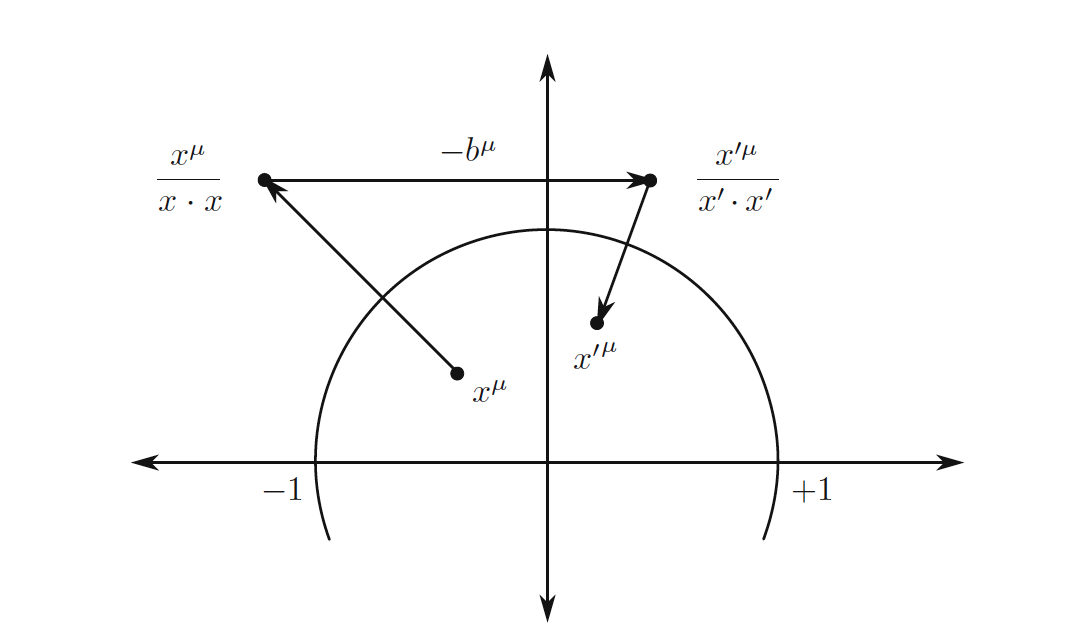
\includegraphics[scale=0.5]{conformal.png}
	\caption{Illustration of a finite SCT}
	%\label{fig_nitjlogo2}
\end{figure}

\section{June 2021 - Poincar\'e commutations}
The matrix of the homogeneous part of Poincar\'e group in the interpolating angle basis may be written as
\bea
\label{matrix}
M_{\wh{\mu}\wh{\nu}} = 
\left[ \begin{array}{cccc}
0 & K^3 & {\mathcal D}^{\wh1} & {\mathcal D}^{\wh2}  \\
-K^3 & 0 & {\mathcal K}^{\wh1} & {\mathcal K}^{\wh2} \\
-{\mathcal D}^{\wh1} & -{\mathcal K}^{\wh1} & 0 & J^3 \\
-{\mathcal D}^{\wh 2}  & -{\mathcal K}^{\wh 2} & -J^3 & 0 
\end{array} \right]
\eea

where 
\bea
\label{generators3}
{\mathcal K}^{\wh1}  =  -K^1\sin\delta-J^2\cos\delta & ; & {\mathcal K}^{\wh 2}  =  J^1\cos\delta-K^2\sin\delta  \nonumber \\
{\mathcal D}^{\wh1}  =  -K^1\cos\delta+J^2\sin\delta & ; & {\mathcal D}^{\wh2}  =  -J^1\sin\delta-K^2\cos\delta \, .  
\eea
The kinematic generators ${\mathcal K}^{\wh j}$ and the dynamic ones ${\mathcal D}^{\wh j}, \, j=(1,\,2)$, can also be written as the combinations of $E^{\wh j}$ and $F^{\wh j}$:
\bea
\label{generators1}
{\mathcal K}^{\wh 1}  =  {\mathbb C}F^{\wh 1} - {\mathbb S}E^{\wh 1} & ; &  {\mathcal K}^{\wh 2} =  {\mathbb C}F^{\wh 2} - {\mathbb S}E^{\wh 2} \nonumber \\
{\mathcal D}^{\wh 1}  =  -{\mathbb S}F^{\wh 1} - {\mathbb C}E^{\wh 1} & ; &  {\mathcal D}^{\wh 2}  =  -{\mathbb S}F^{\wh 2} - {\mathbb C}E^{\wh 2}\, ,
\eea
where
\bea
\label{generators2}
E^{\wh 1}  =  J^2\sin\delta+K^1\cos\delta & ; & E^{\wh 2}  =  K^2\cos\delta-J^1\sin\delta \nonumber\\
F^{\wh 1}  =  K^1\sin\delta-J^2\cos\delta & ; & F^{\wh 2}  =  J^1\cos\delta+K^2\sin\delta \, . 
\eea
Now, the necessary commutation relations for our calculations are
\bea
\left[{\mathcal K}^{\wh{j}}, \, {\mathcal P}_{\wh{+}}\right] & = & -i{\mathbb S}\mathcal P}_{\wh{j}\\
\left[{\mathcal K}^{\wh{j}}, \, {\mathcal P}_{\wh{-}}\right] & = & +i{\mathbb C}\mathcal P}_{\wh{j}\\
\left[{\mathcal K}^{\wh{1}}, \, {\mathcal P}_{\wh{1}}\right] & = & -i\mathcal P}_{\wh{-}\\
\left[{\mathcal K}^{\wh{1}}, \, {\mathcal P}_{\wh{2}}\right] & = & 0\\
\left[{\mathcal K}^{\wh{2}}, \, {\mathcal P}_{\wh{1}}\right] & = & 0\\
\left[{\mathcal K}^{\wh{2}}, \, {\mathcal P}_{\wh{2}}\right] & = & -i\mathcal P}_{\wh{-}\\
\left[{\mathcal D}^{\wh{j}}, \, {\mathcal P}_{\wh{+}}\right] & = & -i{\mathbb C}\mathcal P}_{\wh{j}\\
\left[{\mathcal D}^{\wh{j}}, \, {\mathcal P}_{\wh{-}}\right] & = & -i{\mathbb S}\mathcal P}_{\wh{j}\\
\left[{\mathcal D}^{\wh{1}}, \, {\mathcal P}_{\wh{1}}\right] & = & -i\mathcal P}_{\wh{+}\\
\left[{\mathcal D}^{\wh{1}}, \, {\mathcal P}_{\wh{2}}\right] & = & 0\\
\left[{\mathcal D}^{\wh{2}}, \, {\mathcal P}_{\wh{1}}\right] & = & 0\\
\left[{\mathcal D}^{\wh{2}}, \, {\mathcal P}_{\wh{2}}\right] & = & -i\mathcal P}_{\wh{+}.
\eea



\section{Applying $R_3 = e^{-i\alpha_3 J^3}$ over the momentum operator components}

We apply $R_3 = e^{-i\alpha_3 J^3}$ to each of the momentum operator components $(\wh{\mu} = \wh+,\,\wh- ,\, \wh1,\, \wh2)$:
\bea
R_3^{\dagger} {\mathcal P}_{\wh{\mu}}R_3 & = & e^{i\alpha_3 J^3} {\mathcal P}_{\wh{\mu}} e^{-i\alpha_3 J^3} \nonumber \\
                                 & = & {\mathcal P}_{\wh{\mu}} + i\left[\alpha_3 J^3, {\mathcal P}_{\wh{\mu}} \right] + \frac{i^2}{2!}\left[\alpha_3 J^3, \left[\alpha_3 J^3, {\mathcal P}_{\wh{\mu}} \right]\right] + \frac{i^3}{3!}\left[\alpha_3 J^3,\left[\alpha_3 J^3, \left[\alpha_3 J^3, {\mathcal P}_{\wh{\mu}} \right]\right]\right] + \cdots
\eea
% 
This yields
\begin{align}
\Aboxed{R_3^{\dagger} {\mathcal P}_{\wh+}R_3  = &{\mathcal P}_{\wh+}} \nonumber\\ 
\Aboxed{R_3^{\dagger} {\mathcal P}_{\wh-}R_3  = &{\mathcal P}_{\wh-}} \nonumber\\
R_3^{\dagger} {\mathcal P}^{\wh{1}}R_3  = & {\mathcal P}^{\wh{1}} + i\left[\alpha_3 J^3, {\mathcal P}^{\wh{1}} \right] + \frac{i^2}{2!}\left[\alpha_3 J^3, \left[\alpha_3 J^3, {\mathcal P}^{\wh{1}} \right]\right] + \frac{i^3}{3!}\left[\alpha_3 J^3,\left[\alpha_3 J^3, \left[\alpha_3 J^3, {\mathcal P}^{\wh{1}} \right]\right]\right] + \cdots \nonumber\\
 = & {\mathcal P}^{\wh{1}} - \alpha_3 {\mathcal P}^{\wh{2}} - \frac{1}{2!}\alpha_3^2 {\mathcal P}^{\wh{1}} + \frac{1}{3!}\alpha_3^3{\mathcal P}^{\wh{2}} + \cdots \nonumber\\
\Aboxed{R_3^{\dagger} {\mathcal P}^{\wh{1}}R_3  = & {\mathcal P}^{\wh{1}} \cos{\alpha_3}-{\mathcal P}^{\wh{2}} \sin{\alpha_3}} \nonumber\\
R_3^{\dagger} {\mathcal P}^{\wh{2}}R_3  = & {\mathcal P}^{\wh{2}} + i\left[\alpha_3 J^3, {\mathcal P}^{\wh{2}} \right] + \frac{i^2}{2!}\left[\alpha_3 J^3, \left[\alpha_3 J^3, {\mathcal P}^{\wh{2}} \right]\right] + \frac{i^3}{3!}\left[\alpha_3 J^3,\left[\alpha_3 J^3, \left[\alpha_3 J^3, {\mathcal P}^{\wh{2}} \right]\right]\right] + \cdots \nonumber\\
 = & {\mathcal P}^{\wh{1}} + \alpha_3 {\mathcal P}^{\wh{2}} - \frac{1}{2!}\alpha_3^2 {\mathcal P}^{\wh{1}} - \frac{1}{3!}\alpha_3^3{\mathcal P}^{\wh{2}} + \cdots \nonumber\\
\Aboxed{ R_3^{\dagger} {\mathcal P}^{\wh{2}}R_3  = & {\mathcal P}^{\wh{2}} \cos{\alpha_3}+{\mathcal P}^{\wh{1}} \sin{\alpha_3}} \nonumber\\ \label{T3}
\end{align}
If we apply $R_3$ to the particle momentum state $|P>$, then the particle momentum state is changed to
the state $|P'>$, where $|P>$ and $|P'>$ are the eigenstates of the operator 
${\mathcal P}_{\wh{\mu}}$ with the eigenvalues of  $P_{\wh{\mu}}$ 
and $P'_{\wh{\mu}}$, respectively. From this, one can find that the operation of 
$R_3^{\dagger} {\mathcal P}_{\wh{\mu}}R_3$ and ${\mathcal P}_{\wh{\mu}}$ to the state $|P>$ yields the eigenvalues 
$P'_{\wh{\mu}}$ and $P_{\wh{\mu}}$, respectively.
Thus, the results given in Eq.(\ref{T3}) can be translated into
\bea
\label{T3-eigen}
P'_{\wh+} & = & P_{\wh+}
\nonumber\\ 
P'_{\wh-} & = & P_{\wh-}
\nonumber\\
P'^{\wh{1}} & = & {P}^{\wh{1}}\cos{\alpha_3}-{P}^{\wh{2}} \sin{\alpha_3} \nonumber\\
P'^{\wh{2}} & = & {P}^{\wh{2}}\cos{\alpha_3}+{P}^{\wh{1}} \sin{\alpha_3}
\eea
%
This result satisfies the energy-momentum dispersion relation as it should:
\bea
P'_{\wh \mu}g^{{\wh\mu}{\wh\nu}}P'_{\wh\nu} & = & \mathbb{C}{P'}_{\wh+}^2 + 2\mathbb{S}{P'}_{\wh+} {P'}_{\wh-}-\mathbb{C}{{P'}_{\wh-}}^2-{(P^{\hat1})}^2-{(P^{\hat2})}^2 \nonumber \\
    & = & \mathbb{C}P_{\wh+}^2 + 2\mathbb{S}P_{\wh+}P_{\wh-}-\mathbb{C}P_{\wh-}^2-({P}^{\wh{1}}\cos{\alpha_3}-{P}^{\wh{2}} \sin{\alpha_3})^2 - ({P}^{\wh{2}}\cos{\alpha_3}+{P}^{\wh{1}} \sin{\alpha_3})^2
    \nonumber \\
    & = & \mathbb{C}P_{\wh+}^2 + 2\mathbb{S}P_{\wh+}P_{\wh-}-\mathbb{C}P_{\wh-}^2-({P}^{\wh{1}}\cos{\alpha_3})^2-({P}^{\wh{2}} \sin{\alpha_3})^2 +\cancel{ {P}^{\wh{1}}{P}^{\wh{2}}\cos{\alpha_3}\sin{\alpha_3}}\nonumber \\
    &  &~~~~~~~~~~~~~~~~~~~~~~~~~~~~~~~~~~~~~~~~~~~~~~~~~~~-({P}^{\wh{2}}\cos{\alpha_3})^2-({P}^{\wh{1}} \sin{\alpha_3})^2-\cancel{{P}^{\wh{2}}{P}^{\wh{1}}\cos{\alpha_3} \sin{\alpha_3}}
    \nonumber \\
    & = & \mathbb{C}P_{\wh+}^2 + 2\mathbb{S}P_{\wh+}P_{\wh-}-\mathbb{C}P_{\wh-}^2-({P}^{\wh{1}})^2(\cos{\alpha_3}^2+\sin{\alpha_3}^2)-({P}^{\wh{2}})^2(\cos{\alpha_3}^2+\sin{\alpha_3}^2)
    \nonumber \\
    P'_{\wh \mu}P'^{\wh\nu}& = & \mathbb{C}P_{\wh+}^2 + 2\mathbb{S}P_{\wh+}P_{\wh-}-\mathbb{C}P_{\wh-}^2-{(P^{\hat1})}^2-{(P^{\hat2})}^2
    \nonumber \\
    P'_{\wh \mu}P'^{\wh\nu}&= & M^2 \, .
\eea
%
Taking the limit $\delta \rightarrow 0$ in Eq.(\ref{T3-eigen}), we get
\bea
\label{T3IFD}
P'_{0} & = & P_{0}
\nonumber\\ 
P'_{3} & = & P_{3}
\nonumber\\
P'^{1} & = & {P}^{1}\cos{\alpha_3}-{P}^{2} \sin{\alpha_3} \nonumber\\
P'^{2} & = & {P}^{2}\cos{\alpha_3}+{P}^{1} \sin{\alpha_3} \nonumber
\eea
%
Taking the limit $\delta \rightarrow \frac{\pi}{4}$, on the other hand, we get
\bea
\label{T3LFD}
P'_{+} & = & P_{+}
\nonumber\\ 
P'_{-} & = & P_{-}
\nonumber\\
P'^{{1}} & = & {P}^{{1}}\cos{\alpha_3}-{P}^{{2}} \sin{\alpha_3} \nonumber\\
P'^{{2}} & = & {P}^{{2}}\cos{\alpha_3}+{P}^{{1}} \sin{\alpha_3} \nonumber
\eea
 
This results confirm that $R_3$ is kinematical in both LFD and IFD. 



\section{Applying $T_1 = e^{-i\alpha {\mathcal K}^{\wh{1}} }$ over the momentum operator components}

We apply $T_1 = e^{-i\alpha {\mathcal K}^{\wh{1}} }$ to each of the momentum operator components $(\wh{\mu} = \wh+,\,\wh- ,\, \wh1,\, \wh2)$:
\bea
T_1^{\dagger} {\mathcal P}_{\wh{\mu}}T_1 & = & e^{i\alpha {\mathcal K}^{\wh{1}} } {\mathcal P}_{\wh{\mu}} e^{-i\alpha {\mathcal K}^{\wh{1}} } \nonumber \\
                                 & = & {\mathcal P}_{\wh{\mu}} + i\left[\alpha {\mathcal K}^{\wh{1}}, {\mathcal P}_{\wh{\mu}} \right] + \frac{i^2}{2!}\left[\alpha {\mathcal K}^{\wh{1}}, \left[\alpha {\mathcal K}^{\wh{1}}, {\mathcal P}_{\wh{\mu}} \right]\right] + \frac{i^3}{3!}\left[\alpha {\mathcal K}^{\wh{1}},\left[\alpha {\mathcal K}^{\wh{1}}, \left[\alpha {\mathcal K}^{\wh{1}}, {\mathcal P}_{\wh{\mu}} \right]\right]\right] + \cdots
\eea
% 
This yields
\begin{align}
T_1^{\dagger} {\mathcal P}_{\wh{+}}T_1 & = {\mathcal P}_{\wh{+}} + i\left[\alpha {\mathcal K}^{\wh{1}}, {\mathcal P}_{\wh{+}} \right] + \frac{i^2}{2!}\left[\alpha {\mathcal K}^{\wh{1}}, \left[\alpha {\mathcal K}^{\wh{1}}, {\mathcal P}_{\wh{+}} \right]\right] + \frac{i^3}{3!}\left[\alpha {\mathcal K}^{\wh{1}},\left[\alpha {\mathcal K}^{\wh{1}}, \left[\alpha {\mathcal K}^{\wh{1}}, {\mathcal P}_{\wh{+}} \right]\right]\right] + \cdots \\ %\label{T1}\\
& = {\mathcal P}_{\wh{+}} +\alpha\mathbb S {\mathcal P}_{\wh{1}}  + \frac{\alpha^2}{2!}\mathbb S {\mathcal P}_{\wh{-}} + \frac{\alpha^3}{3!}\mathbb{S}\mathbb{C}{\mathcal P}_{\wh{1}} + \frac{\alpha^4}{4!}\mathbb{S}\mathbb{C}{\mathcal P}_{\wh{-}} + \frac{\alpha^5}{5!}\mathbb{S}\mathbb{C}\mathbb{C}{\mathcal P}_{\wh{1}} + \cdots \\
\Aboxed{ T_1^{\dagger} {\mathcal P}_{{0}}T_1& = {\mathcal P}_{{0}}~~~~~~~~~~~~~~~~~~~~~~~~~~~~~~(IFD)}\\
\Aboxed{T_1^{\dagger} {\mathcal P}_{{+}}T_1& = {\mathcal P}_{{+}}+\alpha {\mathcal P}_{{1}}  + \frac{\alpha^2}{2!} {\mathcal P}_{{-}}~~~~~~~~~~~(LFD)}
\end{align}
\begin{align}
T_1^{\dagger} {\mathcal P}_{\wh{-}}T_1 & = {\mathcal P}_{\wh{-}} + i\left[\alpha {\mathcal K}^{\wh{1}}, {\mathcal P}_{\wh{-}} \right] + \frac{i^2}{2!}\left[\alpha {\mathcal K}^{\wh{1}}, \left[\alpha {\mathcal K}^{\wh{1}}, {\mathcal P}_{\wh{-}} \right]\right] + \frac{i^3}{3!}\left[\alpha {\mathcal K}^{\wh{1}},\left[\alpha {\mathcal K}^{\wh{1}}, \left[\alpha {\mathcal K}^{\wh{1}}, {\mathcal P}_{\wh{-}} \right]\right]\right] + \cdots \\ %\label{T1}\\
& = {\mathcal P}_{\wh{-}} -\alpha\mathbb C {\mathcal P}_{\wh{1}}  - \frac{\alpha^2}{2!}\mathbb C {\mathcal P}_{\wh{-}} + \frac{\alpha^3}{3!}\mathbb{C}{\mathcal P}_{\wh{1}} + \frac{\alpha^4}{4!}\mathbb{C}\mathbb{C}{\mathcal P}_{\wh{-}} - \frac{\alpha^5}{5!}\mathbb{C}\mathbb{C}\mathbb{C}{\mathcal P}_{\wh{1}} + \cdots \\
\Aboxed{T_1^{\dagger} {\mathcal P}_{{3}}T_1& = {\mathcal P}_{{3}} \cos{\alpha}-{\mathcal P}_{{1}}\sin{\alpha}~~~~~~~~~(IFD)}\\
\Aboxed{T_1^{\dagger} {\mathcal P}_{{-}}T_1& = {\mathcal P}_{{-}}~~~~~~~~~~~~~~~~~~~~~~~~~~~~~~(LFD)}
\end{align}

\begin{align}
T_1^{\dagger} {\mathcal P}_{\wh{1}}T_1 & = {\mathcal P}_{\wh{1}} + i\left[\alpha {\mathcal K}^{\wh{1}}, {\mathcal P}_{\wh{1}} \right] + \frac{i^2}{2!}\left[\alpha {\mathcal K}^{\wh{1}}, \left[\alpha {\mathcal K}^{\wh{1}}, {\mathcal P}_{\wh{1}} \right]\right] + \frac{i^3}{3!}\left[\alpha {\mathcal K}^{\wh{1}},\left[\alpha {\mathcal K}^{\wh{1}}, \left[\alpha {\mathcal K}^{\wh{1}}, {\mathcal P}_{\wh{1}} \right]\right]\right] + \cdots \\ %\label{T1}\\
& = {\mathcal P}_{\wh{1}} +\alpha {\mathcal P}_{\wh{-}}  - \frac{\alpha^2}{2!}\mathbb C {\mathcal P}_{\wh{1}} - \frac{\alpha^3}{3!}\mathbb{C}\mathbb{C}{\mathcal P}_{\wh{-}} + \frac{\alpha^4}{4!}\mathbb{C}\mathbb{C}{\mathcal P}_{\wh{1}} + \frac{\alpha^5}{5!}\mathbb{C}\mathbb{C}\mathbb{C}{\mathcal P}_{\wh{-}} + \cdots \\
\Aboxed{T_1^{\dagger} {\mathcal P}_{{1}}T_1 & = {\mathcal P}_{{1}} \cos{\alpha}+{\mathcal P}_{{3}}\sin{\alpha} ~~~~~~~~~(IFD)}\\
\Aboxed{T_1^{\dagger} {\mathcal P}_{{1}}T_1& = {\mathcal P}_{{1}}+\alpha {\mathcal P}_{{-}}~~~~~~~~~~~~~~~~~~~~~(LFD)}
\end{align}

\begin{align}
T_1^{\dagger} {\mathcal P}_{\wh{2}}T_1 & = {\mathcal P}_{\wh{2}} + i\left[\alpha {\mathcal K}^{\wh{1}}, {\mathcal P}_{\wh{2}} \right] + \frac{i^2}{2!}\left[\alpha {\mathcal K}^{\wh{1}}, \left[\alpha {\mathcal K}^{\wh{1}}, {\mathcal P}_{\wh{2}} \right]\right] + \frac{i^3}{3!}\left[\alpha {\mathcal K}^{\wh{1}},\left[\alpha {\mathcal K}^{\wh{1}}, \left[\alpha {\mathcal K}^{\wh{1}}, {\mathcal P}_{\wh{2}} \right]\right]\right] + \cdots \\ %\label{T1}\\
& = {\mathcal P}_{\wh{2}}  \\
\Aboxed{T_1^{\dagger} {\mathcal P}_{{2}}T_1 & = {\mathcal P}_{\wh{2}} ~~~~~~~~~~~~~~~~~~~~~(IFD)}\\
\Aboxed{T_1^{\dagger} {\mathcal P}_{{2}}T_1& = {\mathcal P}_{{2}}~~~~~~~~~~~~~~~~~~~~~(LFD)}\label{T3}
\end{align}
If we apply $T_1$ to the particle momentum state $|P>$, then the particle momentum state is changed to
the state $|P'>$, where $|P>$ and $|P'>$ are the eigenstates of the operator 
${\mathcal P}_{\wh{\mu}}$ with the eigenvalues of  $P_{\wh{\mu}}$ 
and $P'_{\wh{\mu}}$, respectively. From this, one can find that the operation of 
$T_1^{\dagger} {\mathcal P}_{\wh{\mu}}T_1$ and ${\mathcal P}_{\wh{\mu}}$ to the state $|P>$ yields the eigenvalues 
$P'_{\wh{\mu}}$ and $P_{\wh{\mu}}$, respectively.
Taking the limit $\delta \rightarrow 0$ in Eq., we get
\bea
\label{T3IFD}
P'_{0} & = & P_{0}
\nonumber\\ 
P'_{3} & = & {P}_{3}\cos{\alpha}-{P}_{1} \sin{\alpha}
\nonumber\\
P'_{1} & = & {P}_{1}\cos{\alpha}-{P}_{3} \sin{\alpha} \nonumber\\
P'_{2} & = & {P}_{2} \nonumber
\eea
in IFD, $\mathcal{K}^{\hat{1}}$ is the  Transverse Rotation  $-J^2$.\\
%
Taking the limit $\delta \rightarrow \frac{\pi}{4}$, on the other hand, we get
\bea
\label{T3LFD}
P'_{+} & = & P_{+} +\alpha P_{1}+\frac{\alpha^2}{2!}P_{-}
\nonumber\\ 
P'_{-} & = & P_{-}
\nonumber\\
P'_{{1}} & = & {P}_{{1}}+\alpha P_{-} \nonumber\\
P'_{{2}} & = & {P}_{{2}} \nonumber
\eea
in LFD, $\mathcal{K}^{\hat{1}}$ is the LF Transverse Boost  $-E^1$.\\
This result satisfies the energy-momentum dispersion (LFD) relation as it should:
\begin{align}
    P'_{ \mu}g^{{\mu}{\nu}}P'_{\nu}&=2P'_+P'_--P'_1^2-P'_2^2\\
    &=2(P_{+} +\alpha P_{1}+\frac{\alpha^2}{2!}P_{-})(P_{-})-({P}_{{1}}+\alpha P_{-})^2-{P}_{{2}}^2 \\
     &=2P_{+} P_{-}+\cancel{2\alpha P_{1}P_{-}}+\cancel{\alpha^2P_{-}^2}-{P}_{{1}}^2-\cancel{\alpha^2 P_{-}^2}-\cancel{2\alpha {P}_{{1}} P_{-}}-{P}_{{2}}^2\\
     \Aboxed{P'_{ \mu}g^{{\mu}{\nu}}P'_{\nu}&=2P_{+} P_{-}-{P}_{{1}}^2-{P}_{{2}}^2}\checkmark
\end{align}




\section{Applying $T_2 = e^{-i\alpha {\mathcal K}^{\wh{2}} }$ over the momentum operator components}

We apply $T_2 = e^{-i\alpha {\mathcal K}^{\wh{2}} }$ to each of the momentum operator components $(\wh{\mu} = \wh+,\,\wh- ,\, \wh1,\, \wh2)$:
\bea
T_2^{\dagger} {\mathcal P}_{\wh{\mu}}T_2 & = & e^{i\alpha {\mathcal K}^{\wh{2}} } {\mathcal P}_{\wh{\mu}} e^{-i\alpha {\mathcal K}^{\wh{2}} } \nonumber \\
                                 & = & {\mathcal P}_{\wh{\mu}} + i\left[\alpha {\mathcal K}^{\wh{2}}, {\mathcal P}_{\wh{\mu}} \right] + \frac{i^2}{2!}\left[\alpha {\mathcal K}^{\wh{2}}, \left[\alpha {\mathcal K}^{\wh{2}}, {\mathcal P}_{\wh{\mu}} \right]\right] + \frac{i^3}{3!}\left[\alpha {\mathcal K}^{\wh{2}},\left[\alpha {\mathcal K}^{\wh{2}}, \left[\alpha {\mathcal K}^{\wh{2}}, {\mathcal P}_{\wh{\mu}} \right]\right]\right] + \cdots
\eea
% 
This yields
\begin{align}
T_2^{\dagger} {\mathcal P}_{\wh{+}}T_2 & = {\mathcal P}_{\wh{+}} + i\left[\alpha {\mathcal K}^{\wh{2}}, {\mathcal P}_{\wh{+}} \right] + \frac{i^2}{2!}\left[\alpha {\mathcal K}^{\wh{2}}, \left[\alpha {\mathcal K}^{\wh{2}}, {\mathcal P}_{\wh{+}} \right]\right] + \frac{i^3}{3!}\left[\alpha {\mathcal K}^{\wh{2}},\left[\alpha {\mathcal K}^{\wh{2}}, \left[\alpha {\mathcal K}^{\wh{2}}, {\mathcal P}_{\wh{+}} \right]\right]\right] + \cdots \\ %\label{T1}\\
& = {\mathcal P}_{\wh{+}} +\alpha\mathbb S {\mathcal P}_{\wh{2}}  + \frac{\alpha^2}{2!}\mathbb S {\mathcal P}_{\wh{-}} + \frac{\alpha^3}{3!}\mathbb{S}\mathbb{C}{\mathcal P}_{\wh{2}} + \frac{\alpha^4}{4!}\mathbb{S}\mathbb{C}{\mathcal P}_{\wh{-}} + \frac{\alpha^5}{5!}\mathbb{S}\mathbb{C}\mathbb{C}{\mathcal P}_{\wh{2}} + \cdots \\
\Aboxed{ T_2^{\dagger} {\mathcal P}_{{0}}T_2& = {\mathcal P}_{{0}}~~~~~~~~~~~~~~~~~~~~~~~~~~~~~~(IFD)}\\
\Aboxed{T_2^{\dagger} {\mathcal P}_{{+}}T_2& = {\mathcal P}_{{+}}+\alpha {\mathcal P}_{{2}}  + \frac{\alpha^2}{2!} {\mathcal P}_{{-}}~~~~~~~~~~~(LFD)}
\end{align}
\begin{align}
T_2^{\dagger} {\mathcal P}_{\wh{-}}T_2 & = {\mathcal P}_{\wh{-}} + i\left[\alpha {\mathcal K}^{\wh{2}}, {\mathcal P}_{\wh{-}} \right] + \frac{i^2}{2!}\left[\alpha {\mathcal K}^{\wh{2}}, \left[\alpha {\mathcal K}^{\wh{2}}, {\mathcal P}_{\wh{-}} \right]\right] + \frac{i^3}{3!}\left[\alpha {\mathcal K}^{\wh{2}},\left[\alpha {\mathcal K}^{\wh{2}}, \left[\alpha {\mathcal K}^{\wh{2}}, {\mathcal P}_{\wh{-}} \right]\right]\right] + \cdots \\ %\label{T1}\\
& = {\mathcal P}_{\wh{-}} -\alpha\mathbb C {\mathcal P}_{\wh{2}}  - \frac{\alpha^2}{2!}\mathbb C {\mathcal P}_{\wh{-}} + \frac{\alpha^3}{3!}\mathbb{C}{\mathcal P}_{\wh{2}} + \frac{\alpha^4}{4!}\mathbb{C}\mathbb{C}{\mathcal P}_{\wh{-}} - \frac{\alpha^5}{5!}\mathbb{C}\mathbb{C}\mathbb{C}{\mathcal P}_{\wh{2}} + \cdots \\
\Aboxed{T_2^{\dagger} {\mathcal P}_{{3}}T_2& = {\mathcal P}_{{3}} \cos{\alpha}-{\mathcal P}_{{2}}\sin{\alpha}~~~~~~~~~(IFD)}\\
\Aboxed{T_2^{\dagger} {\mathcal P}_{{-}}T_2& = {\mathcal P}_{{-}}~~~~~~~~~~~~~~~~~~~~~~~~~~~~~~(LFD)}
\end{align}

\begin{align}
T_2^{\dagger} {\mathcal P}_{\wh{1}}T_2 & = {\mathcal P}_{\wh{1}} + i\left[\alpha {\mathcal K}^{\wh{2}}, {\mathcal P}_{\wh{1}} \right] + \frac{i^2}{2!}\left[\alpha {\mathcal K}^{\wh{2}}, \left[\alpha {\mathcal K}^{\wh{2}}, {\mathcal P}_{\wh{1}} \right]\right] + \frac{i^3}{3!}\left[\alpha {\mathcal K}^{\wh{2}},\left[\alpha {\mathcal K}^{\wh{2}}, \left[\alpha {\mathcal K}^{\wh{2}}, {\mathcal P}_{\wh{1}} \right]\right]\right] + \cdots \\ %\label{T1}\\
& = {\mathcal P}_{\wh{1}}  \\
\Aboxed{T_2^{\dagger} {\mathcal P}_{{1}}T_2& = {\mathcal P}_{{1}} ~~~~~~~~~~~~~~~~~~~~~(IFD)}\\
\Aboxed{T_2^{\dagger} {\mathcal P}_{{1}}T_2& = {\mathcal P}_{{1}}~~~~~~~~~~~~~~~~~~~~~(LFD)}
\end{align}

\begin{align}
T_2^{\dagger} {\mathcal P}_{\wh{2}}T_2 & = {\mathcal P}_{\wh{2}} + i\left[\alpha {\mathcal K}^{\wh{2}}, {\mathcal P}_{\wh{2}} \right] + \frac{i^2}{2!}\left[\alpha {\mathcal K}^{\wh{2}}, \left[\alpha {\mathcal K}^{\wh{2}}, {\mathcal P}_{\wh{2}} \right]\right] + \frac{i^3}{3!}\left[\alpha {\mathcal K}^{\wh{2}},\left[\alpha {\mathcal K}^{\wh{2}}, \left[\alpha {\mathcal K}^{\wh{2}}, {\mathcal P}_{\wh{2}} \right]\right]\right] + \cdots \\ %\label{T1}\\
& = {\mathcal P}_{\wh{2}} +\alpha {\mathcal P}_{\wh{-}}  - \frac{\alpha^2}{2!}\mathbb C {\mathcal P}_{\wh{2}} - \frac{\alpha^3}{3!}\mathbb{C}\mathbb{C}{\mathcal P}_{\wh{-}} + \frac{\alpha^4}{4!}\mathbb{C}\mathbb{C}{\mathcal P}_{\wh{2}} + \frac{\alpha^5}{5!}\mathbb{C}\mathbb{C}\mathbb{C}{\mathcal P}_{\wh{-}} + \cdots \\
\Aboxed{T_2^{\dagger} {\mathcal P}_{{2}}T_2& = {\mathcal P}_{{2}} \cos{\alpha}+{\mathcal P}_{{3}} \sin{\alpha} ~~~~~~~~~~~~(IFD)}\\
\Aboxed{T_2^{\dagger} {\mathcal P}_{{2}}T_2& = {\mathcal P}_{{2}}+\alpha {\mathcal P}_{{-}}~~~~~~~~~~~~~~~~~~~~~(LFD)}\label{T3}
\end{align}
If we apply $T_2$ to the particle momentum state $|P>$, then the particle momentum state is changed to
the state $|P'>$, where $|P>$ and $|P'>$ are the eigenstates of the operator 
${\mathcal P}_{\wh{\mu}}$ with the eigenvalues of  $P_{\wh{\mu}}$ 
and $P'_{\wh{\mu}}$, respectively. From this, one can find that the operation of 
$T_2^{\dagger} {\mathcal P}_{\wh{\mu}}T_2$ and ${\mathcal P}_{\wh{\mu}}$ to the state $|P>$ yields the eigenvalues 
$P'_{\wh{\mu}}$ and $P_{\wh{\mu}}$, respectively.
Taking the limit $\delta \rightarrow 0$ in Eq, we get
\bea
\label{T3IFD}
P'_{0} & = & P_{0}
\nonumber\\ 
P'_{3} & = & {P}_{3}\cos{\alpha}-{P}_{2} \sin{\alpha}
\nonumber\\
P'_{1} & = &  {P}_{1} \nonumber\\
P'_{2} & = &  {P}_{2}\cos{\alpha}-{P}_{3} \sin{\alpha} \nonumber
\eea
in IFD, $\mathcal{K}^{\hat{2}}$ is the  Transverse Rotation  $-J^1$.\\
%
Taking the limit $\delta \rightarrow \frac{\pi}{4}$, on the other hand, we get
\bea
\label{T3LFD}
P'_{+} & = & P_{+} +\alpha P_{2}+\frac{\alpha^2}{2!}P_{-}
\nonumber\\ 
P'_{-} & = & P_{-}
\nonumber\\
P'_{{1}} & = & {P}_{{1}} \nonumber\\
P'_{{2}} & = & {P}_{{2}}+\alpha P_{-} \nonumber
\eea
in LFD, $\mathcal{K}^{\hat{2}}$ is the LF Transverse Boost  $-E^2$.\\
This result satisfies the energy-momentum dispersion (LFD) relation as it should:
\begin{align}
    P'_{ \mu}g^{{\mu}{\nu}}P'_{\nu}&=2P'_+P'_--P'_1^2-P'_2^2\\
    &=2(P_{+} +\alpha P_{2}+\frac{\alpha^2}{2!}P_{-})(P_{-})-{P}_{{1}}^2-({P}_{{2}}+\alpha P_{-})^2 \\
     &=2P_{+} P_{-}+\cancel{2\alpha P_{2}P_{-}}+\cancel{\alpha^2P_{-}^2}-{P}_{{1}}^2-{P}_{{2}}^2-\cancel{\alpha^2 P_{-}^2}-\cancel{2\alpha {P}_{{2}} P_{-}}\\
     \Aboxed{P'_{ \mu}g^{{\mu}{\nu}}P'_{\nu}&=2P_{+} P_{-}-{P}_{{1}}^2-{P}_{{2}}^2}\checkmark
\end{align}

\section{Applying $R_1 = e^{-i\alpha {\mathcal D}^{\wh{1}} }$ over the momentum operator components}

We apply $R_1 = e^{-i\alpha {\mathcal D}^{\wh{1}} }$ to each of the momentum operator components $(\wh{\mu} = \wh+,\,\wh- ,\, \wh1,\, \wh2)$:
\bea
R_1^{\dagger} {\mathcal P}_{\wh{\mu}}R_1 & = & e^{i\alpha {\mathcal D}^{\wh{1}} } {\mathcal P}_{\wh{\mu}} e^{-i\alpha {\mathcal D}^{\wh{1}} } \nonumber \\
                                 & = & {\mathcal P}_{\wh{\mu}} + i\left[\alpha {\mathcal D}^{\wh{1}}, {\mathcal P}_{\wh{\mu}} \right] + \frac{i^2}{2!}\left[\alpha {\mathcal D}^{\wh{1}}, \left[\alpha {\mathcal D}^{\wh{1}}, {\mathcal P}_{\wh{\mu}} \right]\right] + \frac{i^3}{3!}\left[\alpha {\mathcal D}^{\wh{1}},\left[\alpha {\mathcal D}^{\wh{1}}, \left[\alpha {\mathcal D}^{\wh{1}}, {\mathcal P}_{\wh{\mu}} \right]\right]\right] + \cdots
\eea
% 
This yields
\begin{align}
R_1^{\dagger} {\mathcal P}_{\wh{+}}R_1 & = {\mathcal P}_{\wh{+}} + i\left[\alpha {\mathcal D}^{\wh{1}}, {\mathcal P}_{\wh{+}} \right] + \frac{i^2}{2!}\left[\alpha {\mathcal D}^{\wh{1}}, \left[\alpha {\mathcal D}^{\wh{1}}, {\mathcal P}_{\wh{+}} \right]\right] + \frac{i^3}{3!}\left[\alpha {\mathcal D}^{\wh{1}},\left[\alpha {\mathcal D}^{\wh{1}}, \left[\alpha {\mathcal D}^{\wh{1}}, {\mathcal P}_{\wh{+}} \right]\right]\right] + \cdots \\ %\label{T1}\\
& = {\mathcal P}_{\wh{+}} +\alpha\mathbb C {\mathcal P}_{\wh{1}}  + \frac{\alpha^2}{2!}\mathbb C {\mathcal P}_{\wh{+}} + \frac{\alpha^3}{3!}\mathbb{C}\mathbb{C}{\mathcal P}_{\wh{1}} + \frac{\alpha^4}{4!}\mathbb{C}\mathbb{C}{\mathcal P}_{\wh{+}} + \frac{\alpha^5}{5!}\mathbb{C}\mathbb{C}\mathbb{C}{\mathcal P}_{\wh{1}} + \cdots \\
\Aboxed{ R_1^{\dagger} {\mathcal P}_{{0}}R_1& = {\mathcal P}_{{0}}\cosh{\alpha}+\mathcal{P}_{1}\sinh{\alpha}~~~~~~~(IFD)}\\
\Aboxed{R_1^{\dagger} {\mathcal P}_{{+}}R_1& = {\mathcal P}_{{+}}~~~~~~~~~~~~~~~~~~~~~~~~~~~~~~(LFD)}
\end{align}
\begin{align}
{\mathcal P}_{\wh{-}}'& = {\mathcal P}_{\wh{-}} +\alpha\mathbb S {\mathcal P}_{\wh{1}}  + \frac{\alpha^2}{2!}\mathbb C {\mathcal P}_{\wh{+}} + \frac{\alpha^3}{3!}\mathbb{S}\mathbb{C}{\mathcal P}_{\wh{1}} + \cdots \\
\Aboxed{{\mathcal P}_{{3}}'& = {\mathcal P}_{{3}}~~~~~~~~~~~~~~~~~~~~~~~~~~(IFD)}\\
\Aboxed{{\mathcal P}_{{-}}'& = {\mathcal P}_{{-}}+ {\alpha}{\mathcal P}_{{1}}+\frac{\alpha^2}{2!}{\mathcal P}_{{+}}~~~~~(LFD)}
\end{align}

\begin{align}
{\mathcal P}_{\wh{1}}'& = {\mathcal P}_{\wh{1}} +\alpha {\mathcal P}_{\wh{+}}  + \frac{\alpha^2}{2!}\mathbb C {\mathcal P}_{\wh{1}} + \frac{\alpha^3}{3!}\mathbb{C}\mathbb{C}{\mathcal P}_{\wh{+}} + \frac{\alpha^4}{4!}\mathbb{C}\mathbb{C}{\mathcal P}_{\wh{1}} + \frac{\alpha^5}{5!}\mathbb{C}\mathbb{C}\mathbb{C}{\mathcal P}_{\wh{+}} + \cdots \\
\Aboxed{ {\mathcal P}_{{1}}'& = {\mathcal P}_{{1}}\cosh{\alpha}+\mathcal{P}_{0}\sinh{\alpha}~~~~~~~~~~(IFD)}\\
\Aboxed{{\mathcal P}_{{1}}'& = {\mathcal P}_{{1}}+\alpha{\mathcal P}_{{+}}~~~~~~~~~~~~~~~~~~~~~~~~(LFD)}
\end{align}

Similarly,
\begin{align}
\Aboxed{{\mathcal P}_{{2}}'& = {\mathcal P}_{{2}} ~~~~~~~~~~~~~~~~~~~~~(IFD)}\\
\Aboxed{{\mathcal P}_{{2}}'& = {\mathcal P}_{{2}}~~~~~~~~~~~~~~~~~~~~~(LFD)}\label{T3}
\end{align}
If we apply $R_1$ to the particle momentum state $|P>$, then the particle momentum state is changed to
the state $|P'>$, where $|P>$ and $|P'>$ are the eigenstates of the operator 
${\mathcal P}_{\wh{\mu}}$ with the eigenvalues of  $P_{\wh{\mu}}$ 
and $P'_{\wh{\mu}}$, respectively. From this, one can find that the operation of 
$R_1^{\dagger} {\mathcal P}_{\wh{\mu}}R_1$ and ${\mathcal P}_{\wh{\mu}}$ to the state $|P>$ yields the eigenvalues 
$P'_{\wh{\mu}}$ and $P_{\wh{\mu}}$, respectively.
Taking the limit $\delta \rightarrow 0$ in Eq., we get
\bea
\label{T3IFD}
P'_{0} & = & P_{0} \cosh{\alpha}+P_1\sinh{\alpha}
\nonumber\\ 
P'_{3} & = & {P}_{3}
\nonumber\\
P'_{1} & = & P_{1} \cosh{\alpha}+P_0\sinh{\alpha} \nonumber\\
P'_{2} & = & {P}_{2} \nonumber
\eea
in IFD, $\mathcal{D}^{\hat{1}}$ is the  Transverse Boost  $-K^1$.\\
%
Taking the limit $\delta \rightarrow \frac{\pi}{4}$, on the other hand, we get
\bea
\label{T3LFD}
P'_{+} & = & P_{+}
\nonumber\\ 
P'_{-} & = & P_{-}+\alpha P_1+\frac{\alpha^2}{2!}P_+
\nonumber\\
P'_{{1}} & = & {P}_{{1}}+\alpha P_{+} \nonumber\\
P'_{{2}} & = & {P}_{{2}} \nonumber
\eea
in LFD, $\mathcal{D}^{\hat{1}}$ is the LF Transverse Rotation  $-F^1$.\\
This result satisfies the energy-momentum dispersion (LFD) relation as it should:
\begin{align}
    P'_{ \mu}g^{{\mu}{\nu}}P'_{\nu}&=2P'_+P'_--P'_1^2-P'_2^2\\
    &=2(P_{+})(P_{-} +\alpha P_{1}+\frac{\alpha^2}{2!}P_{+})-({P}_{{1}}+\alpha P_{+})^2-{P}_{{2}}^2 \\
     &=2P_{+} P_{-}+\cancel{2\alpha P_{1}P_{+}}+\cancel{\alpha^2P_{+}^2}-{P}_{{1}}^2-\cancel{\alpha^2 P_{+}^2}-\cancel{2\alpha {P}_{{1}} P_{+}}-{P}_{{2}}^2\\
     \Aboxed{P'_{ \mu}g^{{\mu}{\nu}}P'_{\nu}&=2P_{+} P_{-}-{P}_{{1}}^2-{P}_{{2}}^2}\checkmark
\end{align}
\section{Applying $R_2 = e^{-i\alpha {\mathcal D}^{\wh{2}} }$ over the momentum operator components}
Following the same procedure:
Taking the limit $\delta \rightarrow 0$ in Eq., we get
\bea
\label{T3IFD}
P'_{0} & = & P_{0} \cosh{\alpha}+P_2\sinh{\alpha}
\nonumber\\ 
P'_{3} & = & {P}_{3}
\nonumber\\
P'_{1} & = & P_{1} \nonumber\\
P'_{2} & = & P_{2} \cosh{\alpha}+P_0\sinh{\alpha} \nonumber
\eea
in IFD, $\mathcal{D}^{\hat{2}}$ is the  Transverse Boost  $-K^2$.\\
%
Taking the limit $\delta \rightarrow \frac{\pi}{4}$, on the other hand, we get
\bea
\label{T3LFD}
P'_{+} & = & P_{+}
\nonumber\\ 
P'_{-} & = & P_{-}+\alpha P_2+\frac{\alpha^2}{2!}P_+
\nonumber\\
P'_{{1}} & = & {P}_{{1}} \nonumber\\
P'_{{2}} & = & {P}_{{2}}+\alpha P_{+} \nonumber
\eea
in LFD, $\mathcal{D}^{\hat{2}}$ is the LF Transverse Rotation  $-F^2$.
\section{Comprehensive table}
The following table contains the transformation of each momentum operator components under all kinematic and dynamic generators in IFD and LFD:
\begin{center}
\scalebox{1.42}{
\begin{tabular}{ |c|c|c|} 
 \hline
 \rule{0pt}{16pt}  \textbf{Generators} & \textbf{IFD} &\textbf{ LFD}  \\
  \hline
 \rule{0pt}{16pt}  \textbf{$K^3$} &$ \begin{aligned}
 P'^0 & = \cosh\beta_3P^0+\sinh\beta_3P^3 \\ 
P'^3 & = \cosh\beta_3P^3+\sinh\beta_3P^0 \\
P'^j & = P^j, \:\: (j=1,\, 2)
 \end{aligned}$&$ \begin{aligned}
 P'_+ & = {\rm e}^{-\beta_3}P^{-} \\ 
P'_-& = {\rm e}^{\beta_3}P^{+} \\
P'^j & = P^j, \:\: (j=1,\,2)
 \end{aligned}$\\
 \hline 
 \rule{0pt}{16pt}\textbf{$J^3$} &$ \begin{aligned}
 P'_{0} & = P_{0}
\nonumber\\ 
P'_{3} & = P_{3}
\nonumber\\
P'^{1} & = {P}^{1}\cos{\alpha_3}-{P}^{2} \sin{\alpha_3} \nonumber\\
P'^{2} & = {P}^{2}\cos{\alpha_3}+{P}^{1} \sin{\alpha_3} \nonumber
 \end{aligned}$&$ \begin{aligned}
 P'_{+} & = P_{+}
\nonumber\\ 
P'_{-} & =  P_{-}
\nonumber\\
P'^{{1}} & =  {P}^{{1}}\cos{\alpha_3}-{P}^{{2}} \sin{\alpha_3} \nonumber\\
P'^{{2}} & =  {P}^{{2}}\cos{\alpha_3}+{P}^{{1}} \sin{\alpha_3} \nonumber
 \end{aligned}$\\
 \hline 
 \rule{0pt}{16pt}\textbf{$\mathcal{K}^\wh1$} &$ \begin{aligned}
 P'_{0} & =  P_{0}
\nonumber\\ 
P'_{3} & =  {P}_{3}\cos{\alpha}-{P}_{1} \sin{\alpha}
\nonumber\\
P'_{1} & = {P}_{1}\cos{\alpha}-{P}_{3} \sin{\alpha} \nonumber\\
P'_{2} & =  {P}_{2} \nonumber
 \end{aligned}$&$ \begin{aligned}
 P'_{+} & = P_{+} +\alpha P_{1}+\frac{\alpha^2}{2!}P_{-}
\nonumber\\ 
P'_{-} & = P_{-}
\nonumber\\
P'_{{1}} & = {P}_{{1}}+\alpha P_{-} \nonumber\\
P'_{{2}} & =  {P}_{{2}} \nonumber
 \end{aligned}$\\
 \hline 
 \rule{0pt}{16pt}\textbf{$\mathcal{K}^\wh2$} &$ \begin{aligned}
 P'_{0} & = P_{0}
\nonumber\\ 
P'_{3} & =  {P}_{3}\cos{\alpha}-{P}_{2} \sin{\alpha}
\nonumber\\
P'_{1} & =  {P}_{1} \nonumber\\
P'_{2} & =  {P}_{2}\cos{\alpha}-{P}_{3} \sin{\alpha} \nonumber
 \end{aligned}$&$ \begin{aligned}
 P'_{+} & =  P_{+} +\alpha P_{2}+\frac{\alpha^2}{2!}P_{-}
\nonumber\\ 
P'_{-} & =  P_{-}
\nonumber\\
P'_{{1}} & =  {P}_{{1}} \nonumber\\
P'_{{2}} & = {P}_{{2}}+\alpha P_{-} \nonumber
 \end{aligned}$\\
 \hline 
 \rule{0pt}{16pt}\textbf{$\mathcal{D}^\wh1$} &$ \begin{aligned}
 P'_{0} & =  P_{0} \cosh{\alpha}+P_1\sinh{\alpha}
\nonumber\\ 
P'_{3} & =  {P}_{3}
\nonumber\\
P'_{1} & =  P_{1} \cosh{\alpha}+P_0\sinh{\alpha} \nonumber\\
P'_{2} & =  {P}_{2} \nonumber
 \end{aligned}$&$ \begin{aligned}
 P'_{+} & =  P_{+}
\nonumber\\ 
P'_{-} & =  P_{-}+\alpha P_1+\frac{\alpha^2}{2!}P_+
\nonumber\\
P'_{{1}} & =  {P}_{{1}}+\alpha P_{+} \nonumber\\
P'_{{2}} & =  {P}_{{2}} \nonumber
 \end{aligned}$\\
 \hline 
 \rule{0pt}{16pt}\textbf{$\mathcal{D}^\wh2$} &$ \begin{aligned}
 P'_{0} & = P_{0} \cosh{\alpha}+P_2\sinh{\alpha}
\nonumber\\ 
P'_{3} & =  {P}_{3}
\nonumber\\
P'_{1} & =  P_{1} \nonumber\\
P'_{2} & =  P_{2} \cosh{\alpha}+P_0\sinh{\alpha} \nonumber
 \end{aligned}$&$ \begin{aligned}
 P'_{+} & =  P_{+}
\nonumber\\ 
P'_{-} & =  P_{-}+\alpha P_2+\frac{\alpha^2}{2!}P_+
\nonumber\\
P'_{{1}} & =  {P}_{{1}} \nonumber\\
P'_{{2}} & =  {P}_{{2}}+\alpha P_{+} \nonumber
 \end{aligned}$\\
 \hline 
\end{tabular}}
%\caption{Full Conformal algebra in the Interpolation form}
\end{center}





%%%%%%%%%%%%%%






\section{Applying $ e^{-i\alpha D }$ over the space-time components}
\begin{align}
    \left[D, x^{\hat{\mu}}\right]f(x)&=(Dx^{\hat{\mu}}-x^{\hat{\mu}}D)f(x)=-i((x_{\hat{\nu}}\partial^{\hat{\nu}})x^{\hat{\mu}}-x^{\hat{\mu}}(x_{\hat{\nu}}\partial^{\hat{\nu}}))f(x)\\
    &=-ix_{\hat{\nu}}g^{\hat{\mu}{\hat{\nu}}}f(x)=-ix^{\hat{\mu}}f(x)\\
    \Aboxed{\left[D, x^{\hat{\mu}}\right]&=-ix^{\hat{\mu}}}\checkmark
\end{align}
Use, $\left[ D,{\mathcal X}_{\wh{\mu}}\right]=-i{\mathcal X}_{\wh{\mu}}$.
We apply $e^{-i\alpha D$ to each of the space-time components $(\wh{\mu} = \wh+,\,\wh- ,\, \wh1,\, \wh2)$:
\bea
{\mathcal X}_{\wh{\mu}}'& = & e^{i\alpha D} {\mathcal X}_{\wh{\mu}} e^{-i\alpha D } \nonumber \\
& = & {\mathcal X}_{\wh{\mu}} + i\left[\alpha D, {\mathcal X}_{\wh{\mu}} \right] + \frac{i^2}{2!}\left[\alpha D, \left[\alpha D, {\mathcal X}_{\wh{\mu}} \right]\right] + \frac{i^3}{3!}\left[\alpha D,\left[\alpha D, \left[\alpha D, {\mathcal X}_{\wh{\mu}} \right]\right]\right] + \frac{i^4}{4!}\left[\alpha D,\left[\alpha D,\left[\alpha D, \left[\alpha D, {\mathcal X}_{\wh{\mu}} \right]\right]\right]\right]+ \cdots\\
& = & {\mathcal X}_{\wh{\mu}} +\alpha {\mathcal X}_{\wh{\mu}} + \frac{\alpha^2}{2!} {\mathcal X}_{\wh{\mu}}  + \frac{\alpha^3}{3!}{\mathcal X}_{\wh{\mu}} + \frac{\ap\alpha^4}{4!}{\mathcal X}_{\wh{\mu}} + \cdots\\
& = & {\mathcal X}_{\wh{\mu}} (\cosh{\alpha}+\sinh{\alpha})\\
{\mathcal X}_{\wh{\mu}}'& = & {\mathcal X}_{\wh{\mu}} e^{-\alpha}\\
\eea
% 
This yields
\begin{align}
    {\mathcal X}_{\wh{+}}'& =  {\mathcal X}_{\wh{+}} e^{-\alpha}\\
    {\mathcal X}_{\wh{-}}'& =  {\mathcal X}_{\wh{-}} e^{-\alpha}\\
    {\mathcal X}_{\wh{1}}'& =  {\mathcal X}_{\wh{1}} e^{-\alpha}\\
    {\mathcal X}_{\wh{2}}'& =  {\mathcal X}_{\wh{2}} e^{-\alpha}
\end{align}
The states will transform like,
\begin{align}
    \mathcal X\ket{x'}&=x'\ket{x'}\\
    e^{i\alpha D} {\mathcal X}_{\wh{\mu}} e^{-i\alpha D }\ket{x'}&={\mathcal X}_{\wh{\mu}}e^{-\alpha}\ket{x'}\\
    e^{i\alpha D} {\mathcal X}_{\wh{\mu}} e^{-i\alpha D }\ket{x'}&=x'_{\wh{\mu}}e^{-\alpha}\ket{x'}\\
    {\mathcal X}_{\wh{\mu}} e^{-i\alpha D }\ket{x'}&=x'_{\wh{\mu}}e^{-\alpha} e^{-i\alpha D}\ket{x'}\\
    \Longrightarrow~\Aboxed{e^{-i\alpha D }\ket{x'}&=\ket{x'e^{-\alpha}}}
\end{align}
\pagebreak




%%%%%%%%%%%%%%%%%%%%%%%%




\section{Applying $ e^{-ib \mathfrak{K} }$ over the momentum operator components}

\begin{align}
    \left[\mathfrak{K}^{\hat{\mu}},x^{\hat{\nu}}\right]f(x)&=(\mathfrak{K}^{\hat{\mu}}x^{\hat{\nu}}-x^{\hat{\nu}}\mathfrak{K}^{\hat{\mu}})f(x)=-i((\left(2x^{\hat{\mu}}x_{\hat{\rho}}\partial^{\hat{\rho}}-x^2\partial^{\hat{\mu}}\right)x^{\hat{\nu}}-x^{\hat{\nu}}\left(2x^{\hat{\mu}}x_{\hat{\rho}}\partial^{\hat{\rho}}-x^2\partial^{\hat{\mu}}\right)))f(x)\\
    &=-i\left(2x^{\hat{\mu}}x_{\hat{\rho}}\partial^{\hat{\rho}}x^{\hat{\nu}}-x^2\partial^{\hat{\mu}}x^{\hat{\nu}}\right)f(x)\\
    &=-i\left(2x^{\hat{\mu}}x_{\hat{\rho}}g^{\hat{\rho}\hat{\nu}}-x^2g^{\hat{\mu}\hat{\nu}}\right)f(x)\\
    &=-i\left(2x^{\hat{\mu}}x^{\hat{\nu}}-x^2g^{\hat{\mu}\hat{\nu}}\right)f(x)\\
    \Aboxed{\left[\mathfrak{K}^{\hat{\mu}},x^{\hat{\nu}}\right]&=-i\left(2x^{\hat{\mu}}x^{\hat{\nu}}-x^2g^{\hat{\mu}\hat{\nu}}\right)}
\end{align}
\begin{align}
    \Aboxed{\left[\mathfrak{K}^{1},x^{1}\right]&=-i\left(2x^{1}x^{1}-(x^\alpha.x_\alpha)\right)}
\end{align}
Use, $\left[\mathfrak{K}^{1},x^{1}\right]&=-i\left(2x^{1}x^{1}-(x^\alpha.x_\alpha)\right)$.
We apply $e^{ib \mathfrak{K}_{{1}}}$ to each of the space-time components $(\wh{\mu} = \wh+,\,\wh- ,\, \wh1,\, \wh2)$:
\bea
{x}_{{1}}'& = & e^{ib \mathfrak{K}_{{1}}} {x}_{\wh{1}} e^{-ib \mathfrak{K}_{{1}} } \nonumber \\
& = & {x}_{{1}} + i\left[b \mathfrak{K}_{{1}}, {x}_{{1}} \right] + \frac{i^2}{2!}\left[b \mathfrak{K}_{{1}}, \left[b \mathfrak{K}_{{1}}, {x}_{{1}} \right]\right] + \cdots\\
{x}_{{1}}' & = & {x}_{{1}} +b(2x_{1}x_{1}-(x^\alpha.x_\alpha))+ {b^2}(8x_{1}x_{1}x_{1}-2x_{1}(x^\alpha.x_\alpha))+ \cdots
\eea
% 




\section{Sep 2021 - Poincar\'e commutations}
The matrix of the homogeneous part of Poincar\'e group in the interpolating angle basis may be written as
\bea
\label{matrix}
M_{\wh{\mu}\wh{\nu}} = 
\left[ \begin{array}{cccc}
0 & K^3 & {\mathcal D}^{\wh1} & {\mathcal D}^{\wh2}  \\
-K^3 & 0 & {\mathcal K}^{\wh1} & {\mathcal K}^{\wh2} \\
-{\mathcal D}^{\wh1} & -{\mathcal K}^{\wh1} & 0 & J^3 \\
-{\mathcal D}^{\wh 2}  & -{\mathcal K}^{\wh 2} & -J^3 & 0 
\end{array} \right]
\eea

where 
\bea
\label{generators3}
{\mathcal K}^{\wh1}  =  -K^1\sin\delta-J^2\cos\delta & ; & {\mathcal K}^{\wh 2}  =  J^1\cos\delta-K^2\sin\delta  \nonumber \\
{\mathcal D}^{\wh1}  =  -K^1\cos\delta+J^2\sin\delta & ; & {\mathcal D}^{\wh2}  =  -J^1\sin\delta-K^2\cos\delta \, .  
\eea
The kinematic generators ${\mathcal K}^{\wh j}$ and the dynamic ones ${\mathcal D}^{\wh j}, \, j=(1,\,2)$, can also be written as the combinations of $E^{\wh j}$ and $F^{\wh j}$:
\bea
\label{generators1}
{\mathcal K}^{\wh 1}  =  {\mathbb C}F^{\wh 1} - {\mathbb S}E^{\wh 1} & ; &  {\mathcal K}^{\wh 2} =  {\mathbb C}F^{\wh 2} - {\mathbb S}E^{\wh 2} \nonumber \\
{\mathcal D}^{\wh 1}  =  -{\mathbb S}F^{\wh 1} - {\mathbb C}E^{\wh 1} & ; &  {\mathcal D}^{\wh 2}  =  -{\mathbb S}F^{\wh 2} - {\mathbb C}E^{\wh 2}\, ,
\eea
where
\bea
\label{generators2}
E^{\wh 1}  =  J^2\sin\delta+K^1\cos\delta & ; & E^{\wh 2}  =  K^2\cos\delta-J^1\sin\delta \nonumber\\
F^{\wh 1}  =  K^1\sin\delta-J^2\cos\delta & ; & F^{\wh 2}  =  J^1\cos\delta+K^2\sin\delta \, . 
\eea
Now, the necessary commutation relations for our calculations are
\bea
\left[{\mathcal K}^{\wh{j}}, \, {\mathcal P}_{\wh{+}}\right] & = & -i{\mathbb S}\mathcal P}_{\wh{j}\\
\left[{\mathcal K}^{\wh{j}}, \, {\mathcal P}_{\wh{-}}\right] & = & +i{\mathbb C}\mathcal P}_{\wh{j}\\
\left[{\mathcal K}^{\wh{1}}, \, {\mathcal P}_{\wh{1}}\right] & = & -i\mathcal P}_{\wh{-}\\
\left[{\mathcal K}^{\wh{1}}, \, {\mathcal P}_{\wh{2}}\right] & = & 0\\
\left[{\mathcal K}^{\wh{2}}, \, {\mathcal P}_{\wh{1}}\right] & = & 0\\
\left[{\mathcal K}^{\wh{2}}, \, {\mathcal P}_{\wh{2}}\right] & = & -i\mathcal P}_{\wh{-}\\
\left[{\mathcal D}^{\wh{j}}, \, {\mathcal P}_{\wh{+}}\right] & = & -i{\mathbb C}\mathcal P}_{\wh{j}\\
\left[{\mathcal D}^{\wh{j}}, \, {\mathcal P}_{\wh{-}}\right] & = & -i{\mathbb S}\mathcal P}_{\wh{j}\\
\left[{\mathcal D}^{\wh{1}}, \, {\mathcal P}_{\wh{1}}\right] & = & -i\mathcal P}_{\wh{+}\\
\left[{\mathcal D}^{\wh{1}}, \, {\mathcal P}_{\wh{2}}\right] & = & 0\\
\left[{\mathcal D}^{\wh{2}}, \, {\mathcal P}_{\wh{1}}\right] & = & 0\\
\left[{\mathcal D}^{\wh{2}}, \, {\mathcal P}_{\wh{2}}\right] & = & -i\mathcal P}_{\wh{+}.
\eea



\section{Applying $R_3 = e^{-i\alpha_3 J^3}$ over the momentum operator components}

We apply $R_3 = e^{-i\alpha_3 J^3}$ to each of the momentum operator components $(\wh{\mu} = \wh+,\,\wh- ,\, \wh1,\, \wh2)$:
\bea
R_3^{\dagger} {\mathcal P}_{\wh{\mu}}R_3 & = & e^{i\alpha_3 J^3} {\mathcal P}_{\wh{\mu}} e^{-i\alpha_3 J^3} \nonumber \\
                                 & = & {\mathcal P}_{\wh{\mu}} + i\left[\alpha_3 J^3, {\mathcal P}_{\wh{\mu}} \right] + \frac{i^2}{2!}\left[\alpha_3 J^3, \left[\alpha_3 J^3, {\mathcal P}_{\wh{\mu}} \right]\right] + \frac{i^3}{3!}\left[\alpha_3 J^3,\left[\alpha_3 J^3, \left[\alpha_3 J^3, {\mathcal P}_{\wh{\mu}} \right]\right]\right] + \cdots
\eea
% 
This yields
\begin{align}
\Aboxed{R_3^{\dagger} {\mathcal P}_{\wh+}R_3  = &{\mathcal P}_{\wh+}} \nonumber\\ 
\Aboxed{R_3^{\dagger} {\mathcal P}_{\wh-}R_3  = &{\mathcal P}_{\wh-}} \nonumber\\
R_3^{\dagger} {\mathcal P}^{\wh{1}}R_3  = & {\mathcal P}^{\wh{1}} + i\left[\alpha_3 J^3, {\mathcal P}^{\wh{1}} \right] + \frac{i^2}{2!}\left[\alpha_3 J^3, \left[\alpha_3 J^3, {\mathcal P}^{\wh{1}} \right]\right] + \frac{i^3}{3!}\left[\alpha_3 J^3,\left[\alpha_3 J^3, \left[\alpha_3 J^3, {\mathcal P}^{\wh{1}} \right]\right]\right] + \cdots \nonumber\\
 = & {\mathcal P}^{\wh{1}} - \alpha_3 {\mathcal P}^{\wh{2}} - \frac{1}{2!}\alpha_3^2 {\mathcal P}^{\wh{1}} + \frac{1}{3!}\alpha_3^3{\mathcal P}^{\wh{2}} + \cdots \nonumber\\
\Aboxed{R_3^{\dagger} {\mathcal P}^{\wh{1}}R_3  = & {\mathcal P}^{\wh{1}} \cos{\alpha_3}-{\mathcal P}^{\wh{2}} \sin{\alpha_3}} \nonumber\\
R_3^{\dagger} {\mathcal P}^{\wh{2}}R_3  = & {\mathcal P}^{\wh{2}} + i\left[\alpha_3 J^3, {\mathcal P}^{\wh{2}} \right] + \frac{i^2}{2!}\left[\alpha_3 J^3, \left[\alpha_3 J^3, {\mathcal P}^{\wh{2}} \right]\right] + \frac{i^3}{3!}\left[\alpha_3 J^3,\left[\alpha_3 J^3, \left[\alpha_3 J^3, {\mathcal P}^{\wh{2}} \right]\right]\right] + \cdots \nonumber\\
 = & {\mathcal P}^{\wh{1}} + \alpha_3 {\mathcal P}^{\wh{2}} - \frac{1}{2!}\alpha_3^2 {\mathcal P}^{\wh{1}} - \frac{1}{3!}\alpha_3^3{\mathcal P}^{\wh{2}} + \cdots \nonumber\\
\Aboxed{ R_3^{\dagger} {\mathcal P}^{\wh{2}}R_3  = & {\mathcal P}^{\wh{2}} \cos{\alpha_3}+{\mathcal P}^{\wh{1}} \sin{\alpha_3}} \nonumber\\ \label{T3}
\end{align}
If we apply $R_3$ to the particle momentum state $|P>$, then the particle momentum state is changed to
the state $|P'>$, where $|P>$ and $|P'>$ are the eigenstates of the operator 
${\mathcal P}_{\wh{\mu}}$ with the eigenvalues of  $P_{\wh{\mu}}$ 
and $P'_{\wh{\mu}}$, respectively. From this, one can find that the operation of 
$R_3^{\dagger} {\mathcal P}_{\wh{\mu}}R_3$ and ${\mathcal P}_{\wh{\mu}}$ to the state $|P>$ yields the eigenvalues 
$P'_{\wh{\mu}}$ and $P_{\wh{\mu}}$, respectively.
Thus, the results given in Eq.(\ref{T3}) can be translated into
\bea
\label{T3-eigen}
P'_{\wh+} & = & P_{\wh+}
\nonumber\\ 
P'_{\wh-} & = & P_{\wh-}
\nonumber\\
P'^{\wh{1}} & = & {P}^{\wh{1}}\cos{\alpha_3}-{P}^{\wh{2}} \sin{\alpha_3} \nonumber\\
P'^{\wh{2}} & = & {P}^{\wh{2}}\cos{\alpha_3}+{P}^{\wh{1}} \sin{\alpha_3}
\eea
%
This result satisfies the energy-momentum dispersion relation as it should:
\bea
P'_{\wh \mu}g^{{\wh\mu}{\wh\nu}}P'_{\wh\nu} & = & \mathbb{C}{P'}_{\wh+}^2 + 2\mathbb{S}{P'}_{\wh+} {P'}_{\wh-}-\mathbb{C}{{P'}_{\wh-}}^2-{(P^{\hat1})}^2-{(P^{\hat2})}^2 \nonumber \\
    & = & \mathbb{C}P_{\wh+}^2 + 2\mathbb{S}P_{\wh+}P_{\wh-}-\mathbb{C}P_{\wh-}^2-({P}^{\wh{1}}\cos{\alpha_3}-{P}^{\wh{2}} \sin{\alpha_3})^2 - ({P}^{\wh{2}}\cos{\alpha_3}+{P}^{\wh{1}} \sin{\alpha_3})^2
    \nonumber \\
    & = & \mathbb{C}P_{\wh+}^2 + 2\mathbb{S}P_{\wh+}P_{\wh-}-\mathbb{C}P_{\wh-}^2-({P}^{\wh{1}}\cos{\alpha_3})^2-({P}^{\wh{2}} \sin{\alpha_3})^2 +\cancel{ {P}^{\wh{1}}{P}^{\wh{2}}\cos{\alpha_3}\sin{\alpha_3}}\nonumber \\
    &  &~~~~~~~~~~~~~~~~~~~~~~~~~~~~~~~~~~~~~~~~~~~~~~~~~~~-({P}^{\wh{2}}\cos{\alpha_3})^2-({P}^{\wh{1}} \sin{\alpha_3})^2-\cancel{{P}^{\wh{2}}{P}^{\wh{1}}\cos{\alpha_3} \sin{\alpha_3}}
    \nonumber \\
    & = & \mathbb{C}P_{\wh+}^2 + 2\mathbb{S}P_{\wh+}P_{\wh-}-\mathbb{C}P_{\wh-}^2-({P}^{\wh{1}})^2(\cos{\alpha_3}^2+\sin{\alpha_3}^2)-({P}^{\wh{2}})^2(\cos{\alpha_3}^2+\sin{\alpha_3}^2)
    \nonumber \\
    P'_{\wh \mu}P'^{\wh\nu}& = & \mathbb{C}P_{\wh+}^2 + 2\mathbb{S}P_{\wh+}P_{\wh-}-\mathbb{C}P_{\wh-}^2-{(P^{\hat1})}^2-{(P^{\hat2})}^2
    \nonumber \\
    P'_{\wh \mu}P'^{\wh\nu}&= & M^2 \, .
\eea
%
Taking the limit $\delta \rightarrow 0$ in Eq.(\ref{T3-eigen}), we get
\bea
\label{T3IFD}
P'_{0} & = & P_{0}
\nonumber\\ 
P'_{3} & = & P_{3}
\nonumber\\
P'^{1} & = & {P}^{1}\cos{\alpha_3}-{P}^{2} \sin{\alpha_3} \nonumber\\
P'^{2} & = & {P}^{2}\cos{\alpha_3}+{P}^{1} \sin{\alpha_3} \nonumber
\eea
%
Taking the limit $\delta \rightarrow \frac{\pi}{4}$, on the other hand, we get
\bea
\label{T3LFD}
P'_{+} & = & P_{+}
\nonumber\\ 
P'_{-} & = & P_{-}
\nonumber\\
P'^{{1}} & = & {P}^{{1}}\cos{\alpha_3}-{P}^{{2}} \sin{\alpha_3} \nonumber\\
P'^{{2}} & = & {P}^{{2}}\cos{\alpha_3}+{P}^{{1}} \sin{\alpha_3} \nonumber
\eea
 
This results confirm that $R_3$ is kinematical in both LFD and IFD. 

%%%%%%%%%%%%%%



\section{Oct, 2021 - Applying $e^{-ib^{\mu} \mathfrak{K}_{\mu}}$ over the space-time components}

\begin{align}
    \left[\mathfrak{K}^{\hat{\mu}},x^{\hat{\nu}}\right]f(x)&=(\mathfrak{K}^{\hat{\mu}}x^{\hat{\nu}}-x^{\hat{\nu}}\mathfrak{K}^{\hat{\mu}})f(x)=-i((\left(2x^{\hat{\mu}}x_{\hat{\rho}}\partial^{\hat{\rho}}-x^2\partial^{\hat{\mu}}\right)x^{\hat{\nu}}-x^{\hat{\nu}}\left(2x^{\hat{\mu}}x_{\hat{\rho}}\partial^{\hat{\rho}}-x^2\partial^{\hat{\mu}}\right)))f(x)\\
    &=-i\left(2x^{\hat{\mu}}x_{\hat{\rho}}\partial^{\hat{\rho}}x^{\hat{\nu}}-x^2\partial^{\hat{\mu}}x^{\hat{\nu}}\right)f(x)\\
    &=-i\left(2x^{\hat{\mu}}x_{\hat{\rho}}g^{\hat{\rho}\hat{\nu}}-x^2g^{\hat{\mu}\hat{\nu}}\right)f(x)\\
    &=-i\left(2x^{\hat{\mu}}x^{\hat{\nu}}-x^2g^{\hat{\mu}\hat{\nu}}\right)f(x)\\
    \Aboxed{\left[\mathfrak{K}^{\hat{\mu}},x^{\hat{\nu}}\right]&=-i\left(2x^{\hat{\mu}}x^{\hat{\nu}}-(x^\alpha.x_\alpha)g^{\hat{\mu}\hat{\nu}}\right)}
\end{align}
We apply $e^{-ib^{\mu} \mathfrak{K}_{\mu}}$ to each of the space-time components $(\wh{\mu} = \wh+,\,\wh- ,\, \wh1,\, \wh2)$:
\begin{align}
{x}_{{\nu}}' = & e^{ib^{\mu} \mathfrak{K}_{\mu}} {x}_{{\nu}} e^{-ib^{\mu} \mathfrak{K}_{\mu} } \nonumber \\
 = & {x}_{{\nu}} + i\left[b^{\mu} \mathfrak{K}_{\mu}, {x}_{{\nu}} \right] + \frac{i^2}{2!}\left[b^{\mu} \mathfrak{K}_{\mu}, \left[b^{\mu} \mathfrak{K}_{\mu}, {x}_{{\nu}} \right]\right] + \cdots\\
{x}_{{\nu}}'  = & {x}_{{\nu}} +b^{\mu} (2x_{\hat{\mu}}x_{\hat{\nu}}-(x^\alpha.x_\alpha)g_{\hat{\mu}\hat{\nu}})+ {b^2}(\cdots)+ \cdots\\
{x}_{{\nu}}'  = & {x}_{{\nu}} + 2(b^{\mu}.x_{{\mu}})x_{{\nu}}-b_{\nu}(x^\alpha.x_\alpha)+ \cancelto{0;~~~\text{Since, $b^\nu<<1$}}{\mathcal{O}({b^2})}\\
\Aboxed{x_\nu'  = & {x}_{{\nu}} + 2(b.x)x_{{\nu}}-b_{\nu}x^2}~~~\checkmark
\end{align}
above equation is the infinitesimal SCT.\\
Now,  we  are  going  to  try  to  find  the  finite  conformal  transformation  from  theinfinitesimal one,
\begin{align}
    x'^2&=({x}^{{\nu}} + 2(b.x)x^{{\nu}}-b^{\nu}x^2)({x}_{{\nu}} + 2(b.x)x_{{\nu}}-b_{\nu}x^2)\\
    &=x^2+2x^2(x.b)-x^2(x.b)+2x^2(x.b)+4(x.b)^2x^2-2(x.b)^2x^2-x^2(x.b)-2(x.b)^2x^2+b^2x^2\\
    &=x^2+2(x.b)x^2+b^2x^2
\end{align}
hence $b<<1$,
\begin{align}
    \frac{x'^\nu}{x'^2}&=\frac{{x}^{{\nu}} + 2(b.x)x^{{\nu}}-b^{\nu}x^2}{x^2+2(x.b)x^2+b^2x^2}\\
    &=\frac{1}{x^2}\frac{({x}^{{\nu}} + 2(b.x)x^{{\nu}}-b^{\nu}x^2)}{(1+2(x.b)+b^2)}\\
    &=\frac{1}{x^2}({x}^{{\nu}} + 2(b.x)x^{{\nu}}-b^{\nu}x^2)(1+2(x.b)+b^2)^{-1}\\
    &=\frac{1}{x^2}({x}^{{\nu}} + 2(b.x)x^{{\nu}}-b^{\nu}x^2)(1-2(x.b)-b^2)+\mathcal{O}({b^2})\\
    &=\frac{x^\nu}{x^2}+2(x.b)\frac{x^\nu}{x^2}-b^\nu-2(x.b)\frac{x^\nu}{x^2}+\mathcal{O}({b^2})\\
    &=\frac{x^\nu}{x^2}-b^\nu+\mathcal{O}({b^2})
\end{align}
Now for finite transformation $b^\nu$ we can transform with $\frac{b^\nu}{N}N$ times and take $N$ large.  Hence we have
\begin{align}
    \frac{x'^\nu}{x'^2}&=\frac{x^\nu}{x^2}-\left(\frac{b^\nu}{N}+\mathcal{O}\left({\frac{b^\nu}{N}}\right)^2\right)N\\
    \frac{x'^\nu}{x'^2}&=\frac{x^\nu}{x^2}-b^\nu+\cancelto{0;~~N\to\infty}{\mathcal{O}\left({\frac{b^2}{N}}\right)}
\end{align}
Now, let's square $\frac{x'^\nu}{x'^2}=\frac{x^\nu}{x^2}-b^\nu$
\begin{align}
    \frac{1}{x'^2}&=\frac{1}{x'^2}-\frac{2(b.x)}{x^2}+b^2
\end{align}
Now inverse this, we have
\begin{align}
    x'^2&=\frac{x^2}{1-2(b.x)+b^2x^2}
\end{align}
Now plug this back to $\frac{x'^\nu}{x'^2}=\frac{x^\nu}{x^2}-b^\nu$, and we get
\begin{align}
    x'^\nu&=\frac{x^2}{1-2(b.x)+b^2x^2}\left(\frac{x^\nu}{x^2}-b^\nu\right)\\
    \Aboxed{x'^\nu&=\frac{x^{\nu} - b^{\nu}x^2}{1-2x\cdot b + b^2 x^2}}\checkmark
\end{align}


% 

%%%%%%%%%%%%%%
\section{Nov 2021 - Applying $e^{-ib^{\mu} \mathfrak{K}_{\mu}}$ over the space-time components}

\begin{align}
    \left[\mathfrak{K}^{\hat{\mu}},x^{\hat{\nu}}\right]f(x)&=(\mathfrak{K}^{\hat{\mu}}x^{\hat{\nu}}-x^{\hat{\nu}}\mathfrak{K}^{\hat{\mu}})f(x)=i((\left(2x^{\hat{\mu}}x_{\hat{\rho}}\partial^{\hat{\rho}}-x^2\partial^{\hat{\mu}}\right)x^{\hat{\nu}}-x^{\hat{\nu}}\left(2x^{\hat{\mu}}x_{\hat{\rho}}\partial^{\hat{\rho}}-x^2\partial^{\hat{\mu}}\right)))f(x)\\
    &=i\left(2x^{\hat{\mu}}x_{\hat{\rho}}\partial^{\hat{\rho}}x^{\hat{\nu}}-x^2\partial^{\hat{\mu}}x^{\hat{\nu}}\right)f(x)\\
    &=i\left(2x^{\hat{\mu}}x_{\hat{\rho}}g^{\hat{\rho}\hat{\nu}}-x^2g^{\hat{\mu}\hat{\nu}}\right)f(x)\\
    &=i\left(2x^{\hat{\mu}}x^{\hat{\nu}}-x^2g^{\hat{\mu}\hat{\nu}}\right)f(x)\\
    \Aboxed{\left[\mathfrak{K}^{\hat{\mu}},x^{\hat{\nu}}\right]&=i\left(2x^{\hat{\mu}}x^{\hat{\nu}}-(x^\alpha.x_\alpha)g^{\hat{\mu}\hat{\nu}}\right)}
\end{align}

One can also do this,
 \begin{align}
     \left[\mathfrak{K}^{\hat{\mu}},(x^{\hat{\nu}}x_{\hat{\nu}})\right]f(x)&=(\mathfrak{K}^{\hat{\mu}}x^{2}-x^{2}\mathfrak{K}^{\hat{\mu}})f(x)=i((\left(2x^{\hat{\mu}}x_{\hat{\rho}}\partial^{\hat{\rho}}-x^2\partial^{\hat{\mu}}\right)x^{2}-x^{2}\left(2x^{\hat{\mu}}x_{\hat{\rho}}\partial^{\hat{\rho}}-x^2\partial^{\hat{\mu}}\right)))f(x)\\
     \Aboxed{\left[\mathfrak{K}^{\hat{\mu}},(x^{2})\right]=&i\left(2x^{\hat{\mu}}(x^\alpha.x_\alpha)\right)}
 \end{align}
 
 Let's also find $\left[b^{\mu} \mathfrak{K}_{\mu}, \left[b^{\mu} \mathfrak{K}_{\mu}, {x}_{{\nu}} \right]\right]$,
 \begin{align}
     \left[b^{\mu} \mathfrak{K}_{\mu}, \left[b^{\mu} \mathfrak{K}_{\mu}, {x}_{{\nu}} \right]\right]&=ib^{\mu}b^{\mu}\left[ \mathfrak{K}_{\mu}, \left(2x_{{\mu}}x_{{\nu}}-(x^\alpha.x_\alpha)g_{{\mu}{\nu}}\right)\right]\\
     &=ib^{\mu}b^{\mu}\left(\left[ \mathfrak{K}_{\mu}, \left(2x_{{\mu}}x_{{\nu}}\right)\right]-\left[ \mathfrak{K}_{\mu}, \left(x^\alpha.x_\alpha)g_{{\mu}{\nu}}\right)\right]\right)\\
     &=ib^{\mu}b^{\mu}\left(2\left(\left[ \mathfrak{K}_{\mu}, x_{{\mu}}\right]x_{{\nu}}+x_{{\mu}}\left[ \mathfrak{K}_{\mu},x_{{\nu}}\right]\right)-\left[ \mathfrak{K}_{\mu}, \left(x^\alpha.x_\alpha)g_{{\mu}{\nu}}\right)\right]\right)\\
     &=(-1)b^{\mu}b^{\mu}\left(8x_\mu x_\mu x_\nu - 2 x^2 g_{\mu\mu}x_\nu-4x^2x_\mu g_{\mu}\right)\\
     &=(-1)\left(8(x.b)(x.b)x_\nu-2(x.x)(b.b)x_\nu-4(x.x)(b.x)b_\nu\right)
 \end{align}
Now,\\
We apply $e^{-ib^{\mu} \mathfrak{K}_{\mu}}$ to each of the space-time components $(\wh{\mu} = \wh+,\,\wh- ,\, \wh1,\, \wh2)$:
\begin{align}
{x}_{{\nu}}' = & e^{ib^{\mu} \mathfrak{K}_{\mu}} {x}_{{\nu}} e^{-ib^{\mu} \mathfrak{K}_{\mu} } \nonumber \\
 = & {x}_{{\nu}} + i\left[b^{\mu} \mathfrak{K}_{\mu}, {x}_{{\nu}} \right] + \textcolor{blue}{\frac{i^2}{2!}\left[b^{\mu} \mathfrak{K}_{\mu}, \left[b^{\mu} \mathfrak{K}_{\mu}, {x}_{{\nu}} \right]\right]} + \cdots\\
{x}_{{\nu}}'  = & {x}_{{\nu}} -b^{\mu} (2x_{\hat{\mu}}x_{\hat{\nu}}-(x^\alpha.x_\alpha)g_{\hat{\mu}\hat{\nu}})+\textcolor{blue}{\frac{1}{2}\left(8(x.b)(x.b)x_\nu-2(x.x)(b.b)x_\nu-4(x.x)(b.x)b_\nu\right)} + \cdots\\
\Aboxed{{x}_{{\nu}}'  = & {x}_{{\nu}} - 2(b^{\mu}.x_{{\mu}})x_{{\nu}}+b_{\nu}(x^\alpha.x_\alpha)+\textcolor{blue}{4(x.b)(x.b)x_\nu-(x.x)(b.b)x_\nu-2(x.x)(b.x)b_\nu}+ \cdots\cdots}\checkmark\label{1}
\end{align}
In order to show that the above expression will converge to SCT $x'_\nu=\frac{x_{\nu} - b_{\nu}x^2}{1-2x\cdot b + b^2 x^2}$, Let's take the binomial expansion for SCT,
\begin{align}
    x'_\nu&=\frac{x_{\nu} + b_{\nu}x^2}{1+2x\cdot b + b^2 x^2}\\
    &=({x_{\nu} + b_{\nu}x^2})({1+2x\cdot b + b^2 x^2})^{-1}\\
    &=({x_{\nu} + b_{\nu}x^2})({1-2x\cdot b + b^2 x^2}+4(x.b)(x.b)+\cdots\cdots)\\
    &=  {x}_{{\nu}} +b_{\nu}(x^\alpha.x_\alpha)-2(b^{\mu}.x_{{\mu}})x_{{\nu}}-2(x.x)(b.x)b_\nu-(x.x)(b.b)x_\nu+(b.b)(x.x)(x.x)b_\nu+4(x.b)(x.b)x_\nu+ \cdots\cdots\\
    \Aboxed{{x}_{{\nu}}'  = & {x}_{{\nu}} - 2(b^{\mu}.x_{{\mu}})x_{{\nu}}+b_{\nu}(x^\alpha.x_\alpha)+\textcolor{blue}{4(x.b)(x.b)x_\nu-(x.x)(b.b)x_\nu-2(x.x)(b.x)b_\nu}+(b.b)(x.x)(x.x)b_\nu+ \cdots\cdots}\checkmark\label{2}
\end{align}
From \eqref{1} and \eqref{2}, we can  confirm that $e^{-ib^{\mu} \mathfrak{K}_{\mu}}$ is the Unitary transformation for SCT.
\pagebreak


\section{Applying $e^{-ib^{\mu} \mathfrak{K}_{\mu}}$ over the momentum components}
We already know, $\left[\mathfrak{K}_{{\mu}},P_{{\nu}}\right]&=-2i\left(g_{{\mu}{\nu}}D+M_{{\mu}{\nu}}\right)$, $\left[\mathfrak{K}_{{\mu}},D\right]=-i\mathfrak{K}_{{\mu}}$, $\left[\mathfrak{K}_{{\rho}},M_{{\mu}{\nu}}\right]&=i\left(g_{{\rho}{\mu}}\mathfrak{K}_{{\nu}}-g_{{\rho}{\nu}}\mathfrak{K}_{{\mu}}\right)$, and $\left[\mathfrak{K}_{{\mu}},\mathfrak{K}_{{\nu}}\right]=0$

We apply $e^{-ib^{\mu} \mathfrak{K}_{\mu}}$ to each of the momentum components:
\begin{align}
{P}_{{\nu}}' = & e^{ib^{\mu} \mathfrak{K}_{\mu}} {P}_{{\nu}} e^{-ib^{\mu} \mathfrak{K}_{\mu} } \nonumber \\
 = & {P}_{{\nu}} + i\left[b^{\mu} \mathfrak{K}_{\mu}, {P}_{{\nu}} \right] + \frac{i^2}{2!}\left[b^{\mu} \mathfrak{K}_{\mu}, \left[b^{\mu} \mathfrak{K}_{\mu}, {P}_{{\nu}} \right]\right]+ \frac{i^3}{3!}\left[b^{\mu} \mathfrak{K}_{\mu},\left[b^{\mu} \mathfrak{K}_{\mu}, \left[b^{\mu} \mathfrak{K}_{\mu}, {P}_{{\nu}} \right]\right] \right] + \cdots\\
  = & {P}_{{\nu}} +2b^\mu \left(g_{{\mu}{\nu}}D+M_{{\mu}{\nu}}\right)- \frac{2i^2i}{2!}\left[b^{\mu} \mathfrak{K}_{\mu},\left( b_{\nu}D+b^\mu M_{{\mu}{\nu}}\right)\right]+0 + \cdots\\
  = & {P}_{{\nu}} +2 \left(b_\nu D+b^\mu M_{{\mu}{\nu}}\right)- i^2i\left[b^{\mu} \mathfrak{K}_{\mu},\left( b_{\nu}D+b^\mu M_{{\mu}{\nu}}\right)\right]+ 0+ \cdots\\
  = & {P}_{{\nu}} +2 \left(b_\nu D+b^\mu M_{{\mu}{\nu}}\right)-i^2i b_{\nu}b^{\mu}\left[ \mathfrak{K}_{\mu}, D\right]-i^2ib^\mu b^{\mu}\left[ \mathfrak{K}_{\mu},M_{{\mu}{\nu}}\right]+  \cdots\\
  = & {P}_{{\nu}} +2 \left(b_\nu D+b^\mu M_{{\mu}{\nu}}\right)+ b_{\nu}(b^{\mu}.\mathfrak{K}_{\mu})-b^\mu b^{\mu}\left(g_{{\mu}{\mu}}\mathfrak{K}_{{\nu}}-g_{{\mu}{\nu}}\mathfrak{K}_{{\mu}}\right)+0+\cdots\\
  = & {P}_{{\nu}} +2 \left(b_\nu D+b^\mu M_{{\mu}{\nu}}\right)+ b_{\nu}(b^{\mu}.\mathfrak{K}_{\mu})-(b^\mu b_{\mu})\mathfrak{K}_{{\nu}}+(b^\mu .\mathfrak{K}_{{\mu}})b_{\nu}\\
  \Aboxed{{P}_{{\nu}}' = & {P}_{{\nu}} +2 \left(b_\nu D+b^\mu M_{{\mu}{\nu}}\right)+2 b_{\nu}(b^{\mu}.\mathfrak{K}_{\mu})-(b^\mu b_{\mu})\mathfrak{K}_{{\nu}}}
\end{align}


In (1+1),

\begin{align}
    {P}_{{0}}' = & e^{ib^{0} \mathfrak{K}_{0}} {P}_{{0}} e^{-ib^{0} \mathfrak{K}_{0} }={P}_{{0}} + 2b_{0}D + b_{0}b_{0}\mathfrak{K}_{0}\\
    {P}_{{3}}' = & e^{ib^{0} \mathfrak{K}_{0}} {P}_{{3}} e^{-ib^{0} \mathfrak{K}_{0} }={P}_{{3}} -2b^{0}K^3  -b_0b_0\mathfrak{K}_{3}\\
    {P}_{{0}}' = & e^{ib^{3} \mathfrak{K}_{3}} {P}_{{0}} e^{-ib^{3} \mathfrak{K}_{3} }={P}_{{0}} + 2b^{3} K^3 +b^3b^3\mathfrak{K}_{3}\\
    {P}_{{3}}' = & e^{ib^{3} \mathfrak{K}_{3}} {P}_{{3}} e^{-ib^{3} \mathfrak{K}_{3} }={P}_{{3}} -2b^3D -b^3b^3\mathfrak{K}_{3}
\end{align}

\begin{align}
    {P}_{{+}}' = & e^{ib^{+} \mathfrak{K}_{+}} {P}_{{+}} e^{-ib^{+} \mathfrak{K}_{+} }={P}_{{+}} \\
    {P}_{{-}}' = & e^{ib^{+} \mathfrak{K}_{+}} {P}_{{-}} e^{-ib^{+} \mathfrak{K}_{+} }={P}_{{-}} + 2\sqrt{2}b^{+}D_{+} +2b^{+}b^{+} \mathfrak{K}_{+}\\
    {P}_{{+}}' = & e^{ib^{-} \mathfrak{K}_{-}} {P}_{{+}} e^{-ib^{-} \mathfrak{K}_{-} }={P}_{{+}} +2\sqrt{2}b^{-}D_{-}+2b^{-}b^{-} \mathfrak{K}_{-}\\
    {P}_{{-}}' = & e^{ib^{-} \mathfrak{K}_{-}} {P}_{{-}} e^{-ib^{-} \mathfrak{K}_{-} }={P}_{{-}} 
\end{align}




\section{Applying $T_1 = e^{-i\alpha {\mathcal K}^{\wh{1}} }$ over the momentum operator components}

We apply $T_1 = e^{-i\alpha {\mathcal K}^{\wh{1}} }$ to each of the momentum operator components $(\wh{\mu} = \wh+,\,\wh- ,\, \wh1,\, \wh2)$:
\bea
T_1^{\dagger} {\mathcal P}_{\wh{\mu}}T_1 & = & e^{i\alpha {\mathcal K}^{\wh{1}} } {\mathcal P}_{\wh{\mu}} e^{-i\alpha {\mathcal K}^{\wh{1}} } \nonumber \\
                                 & = & {\mathcal P}_{\wh{\mu}} + i\left[\alpha {\mathcal K}^{\wh{1}}, {\mathcal P}_{\wh{\mu}} \right] + \frac{i^2}{2!}\left[\alpha {\mathcal K}^{\wh{1}}, \left[\alpha {\mathcal K}^{\wh{1}}, {\mathcal P}_{\wh{\mu}} \right]\right] + \frac{i^3}{3!}\left[\alpha {\mathcal K}^{\wh{1}},\left[\alpha {\mathcal K}^{\wh{1}}, \left[\alpha {\mathcal K}^{\wh{1}}, {\mathcal P}_{\wh{\mu}} \right]\right]\right] + \cdots
\eea
% 
This yields
\begin{align}
T_1^{\dagger} {\mathcal P}_{\wh{+}}T_1 & = {\mathcal P}_{\wh{+}} + i\left[\alpha {\mathcal K}^{\wh{1}}, {\mathcal P}_{\wh{+}} \right] + \frac{i^2}{2!}\left[\alpha {\mathcal K}^{\wh{1}}, \left[\alpha {\mathcal K}^{\wh{1}}, {\mathcal P}_{\wh{+}} \right]\right] + \frac{i^3}{3!}\left[\alpha {\mathcal K}^{\wh{1}},\left[\alpha {\mathcal K}^{\wh{1}}, \left[\alpha {\mathcal K}^{\wh{1}}, {\mathcal P}_{\wh{+}} \right]\right]\right] + \cdots \\ %\label{T1}\\
& = {\mathcal P}_{\wh{+}} +\alpha\mathbb S {\mathcal P}_{\wh{1}}  + \frac{\alpha^2}{2!}\mathbb S {\mathcal P}_{\wh{-}} + \frac{\alpha^3}{3!}\mathbb{S}\mathbb{C}{\mathcal P}_{\wh{1}} + \frac{\alpha^4}{4!}\mathbb{S}\mathbb{C}{\mathcal P}_{\wh{-}} + \frac{\alpha^5}{5!}\mathbb{S}\mathbb{C}\mathbb{C}{\mathcal P}_{\wh{1}} + \cdots \\
\Aboxed{ T_1^{\dagger} {\mathcal P}_{{0}}T_1& = {\mathcal P}_{{0}}~~~~~~~~~~~~~~~~~~~~~~~~~~~~~~(IFD)}\\
\Aboxed{T_1^{\dagger} {\mathcal P}_{{+}}T_1& = {\mathcal P}_{{+}}+\alpha {\mathcal P}_{{1}}  + \frac{\alpha^2}{2!} {\mathcal P}_{{-}}~~~~~~~~~~~(LFD)}
\end{align}
\begin{align}
T_1^{\dagger} {\mathcal P}_{\wh{-}}T_1 & = {\mathcal P}_{\wh{-}} + i\left[\alpha {\mathcal K}^{\wh{1}}, {\mathcal P}_{\wh{-}} \right] + \frac{i^2}{2!}\left[\alpha {\mathcal K}^{\wh{1}}, \left[\alpha {\mathcal K}^{\wh{1}}, {\mathcal P}_{\wh{-}} \right]\right] + \frac{i^3}{3!}\left[\alpha {\mathcal K}^{\wh{1}},\left[\alpha {\mathcal K}^{\wh{1}}, \left[\alpha {\mathcal K}^{\wh{1}}, {\mathcal P}_{\wh{-}} \right]\right]\right] + \cdots \\ %\label{T1}\\
& = {\mathcal P}_{\wh{-}} -\alpha\mathbb C {\mathcal P}_{\wh{1}}  - \frac{\alpha^2}{2!}\mathbb C {\mathcal P}_{\wh{-}} + \frac{\alpha^3}{3!}\mathbb{C}{\mathcal P}_{\wh{1}} + \frac{\alpha^4}{4!}\mathbb{C}\mathbb{C}{\mathcal P}_{\wh{-}} - \frac{\alpha^5}{5!}\mathbb{C}\mathbb{C}\mathbb{C}{\mathcal P}_{\wh{1}} + \cdots \\
\Aboxed{T_1^{\dagger} {\mathcal P}_{{3}}T_1& = {\mathcal P}_{{3}} \cos{\alpha}-{\mathcal P}_{{1}}\sin{\alpha}~~~~~~~~~(IFD)}\\
\Aboxed{T_1^{\dagger} {\mathcal P}_{{-}}T_1& = {\mathcal P}_{{-}}~~~~~~~~~~~~~~~~~~~~~~~~~~~~~~(LFD)}
\end{align}

\begin{align}
T_1^{\dagger} {\mathcal P}_{\wh{1}}T_1 & = {\mathcal P}_{\wh{1}} + i\left[\alpha {\mathcal K}^{\wh{1}}, {\mathcal P}_{\wh{1}} \right] + \frac{i^2}{2!}\left[\alpha {\mathcal K}^{\wh{1}}, \left[\alpha {\mathcal K}^{\wh{1}}, {\mathcal P}_{\wh{1}} \right]\right] + \frac{i^3}{3!}\left[\alpha {\mathcal K}^{\wh{1}},\left[\alpha {\mathcal K}^{\wh{1}}, \left[\alpha {\mathcal K}^{\wh{1}}, {\mathcal P}_{\wh{1}} \right]\right]\right] + \cdots \\ %\label{T1}\\
& = {\mathcal P}_{\wh{1}} +\alpha {\mathcal P}_{\wh{-}}  - \frac{\alpha^2}{2!}\mathbb C {\mathcal P}_{\wh{1}} - \frac{\alpha^3}{3!}\mathbb{C}\mathbb{C}{\mathcal P}_{\wh{-}} + \frac{\alpha^4}{4!}\mathbb{C}\mathbb{C}{\mathcal P}_{\wh{1}} + \frac{\alpha^5}{5!}\mathbb{C}\mathbb{C}\mathbb{C}{\mathcal P}_{\wh{-}} + \cdots \\
\Aboxed{T_1^{\dagger} {\mathcal P}_{{1}}T_1 & = {\mathcal P}_{{1}} \cos{\alpha}+{\mathcal P}_{{3}}\sin{\alpha} ~~~~~~~~~(IFD)}\\
\Aboxed{T_1^{\dagger} {\mathcal P}_{{1}}T_1& = {\mathcal P}_{{1}}+\alpha {\mathcal P}_{{-}}~~~~~~~~~~~~~~~~~~~~~(LFD)}
\end{align}

\begin{align}
T_1^{\dagger} {\mathcal P}_{\wh{2}}T_1 & = {\mathcal P}_{\wh{2}} + i\left[\alpha {\mathcal K}^{\wh{1}}, {\mathcal P}_{\wh{2}} \right] + \frac{i^2}{2!}\left[\alpha {\mathcal K}^{\wh{1}}, \left[\alpha {\mathcal K}^{\wh{1}}, {\mathcal P}_{\wh{2}} \right]\right] + \frac{i^3}{3!}\left[\alpha {\mathcal K}^{\wh{1}},\left[\alpha {\mathcal K}^{\wh{1}}, \left[\alpha {\mathcal K}^{\wh{1}}, {\mathcal P}_{\wh{2}} \right]\right]\right] + \cdots \\ %\label{T1}\\
& = {\mathcal P}_{\wh{2}}  \\
\Aboxed{T_1^{\dagger} {\mathcal P}_{{2}}T_1 & = {\mathcal P}_{\wh{2}} ~~~~~~~~~~~~~~~~~~~~~(IFD)}\\
\Aboxed{T_1^{\dagger} {\mathcal P}_{{2}}T_1& = {\mathcal P}_{{2}}~~~~~~~~~~~~~~~~~~~~~(LFD)}\label{T3}
\end{align}
If we apply $T_1$ to the particle momentum state $|P>$, then the particle momentum state is changed to
the state $|P'>$, where $|P>$ and $|P'>$ are the eigenstates of the operator 
${\mathcal P}_{\wh{\mu}}$ with the eigenvalues of  $P_{\wh{\mu}}$ 
and $P'_{\wh{\mu}}$, respectively. From this, one can find that the operation of 
$T_1^{\dagger} {\mathcal P}_{\wh{\mu}}T_1$ and ${\mathcal P}_{\wh{\mu}}$ to the state $|P>$ yields the eigenvalues 
$P'_{\wh{\mu}}$ and $P_{\wh{\mu}}$, respectively.
Taking the limit $\delta \rightarrow 0$ in Eq., we get
\bea
\label{T3IFD}
P'_{0} & = & P_{0}
\nonumber\\ 
P'_{3} & = & {P}_{3}\cos{\alpha}-{P}_{1} \sin{\alpha}
\nonumber\\
P'_{1} & = & {P}_{1}\cos{\alpha}-{P}_{3} \sin{\alpha} \nonumber\\
P'_{2} & = & {P}_{2} \nonumber
\eea
in IFD, $\mathcal{K}^{\hat{1}}$ is the  Transverse Rotation  $-J^2$.\\
%
Taking the limit $\delta \rightarrow \frac{\pi}{4}$, on the other hand, we get
\bea
\label{T3LFD}
P'_{+} & = & P_{+} +\alpha P_{1}+\frac{\alpha^2}{2!}P_{-}
\nonumber\\ 
P'_{-} & = & P_{-}
\nonumber\\
P'_{{1}} & = & {P}_{{1}}+\alpha P_{-} \nonumber\\
P'_{{2}} & = & {P}_{{2}} \nonumber
\eea
in LFD, $\mathcal{K}^{\hat{1}}$ is the LF Transverse Boost  $-E^1$.\\
This result satisfies the energy-momentum dispersion (LFD) relation as it should:
\begin{align}
    P'_{ \mu}g^{{\mu}{\nu}}P'_{\nu}&=2P'_+P'_--P'_1^2-P'_2^2\\
    &=2(P_{+} +\alpha P_{1}+\frac{\alpha^2}{2!}P_{-})(P_{-})-({P}_{{1}}+\alpha P_{-})^2-{P}_{{2}}^2 \\
     &=2P_{+} P_{-}+\cancel{2\alpha P_{1}P_{-}}+\cancel{\alpha^2P_{-}^2}-{P}_{{1}}^2-\cancel{\alpha^2 P_{-}^2}-\cancel{2\alpha {P}_{{1}} P_{-}}-{P}_{{2}}^2\\
     \Aboxed{P'_{ \mu}g^{{\mu}{\nu}}P'_{\nu}&=2P_{+} P_{-}-{P}_{{1}}^2-{P}_{{2}}^2}\checkmark
\end{align}




\section{Applying $T_2 = e^{-i\alpha {\mathcal K}^{\wh{2}} }$ over the momentum operator components}

We apply $T_2 = e^{-i\alpha {\mathcal K}^{\wh{2}} }$ to each of the momentum operator components $(\wh{\mu} = \wh+,\,\wh- ,\, \wh1,\, \wh2)$:
\bea
T_2^{\dagger} {\mathcal P}_{\wh{\mu}}T_2 & = & e^{i\alpha {\mathcal K}^{\wh{2}} } {\mathcal P}_{\wh{\mu}} e^{-i\alpha {\mathcal K}^{\wh{2}} } \nonumber \\
                                 & = & {\mathcal P}_{\wh{\mu}} + i\left[\alpha {\mathcal K}^{\wh{2}}, {\mathcal P}_{\wh{\mu}} \right] + \frac{i^2}{2!}\left[\alpha {\mathcal K}^{\wh{2}}, \left[\alpha {\mathcal K}^{\wh{2}}, {\mathcal P}_{\wh{\mu}} \right]\right] + \frac{i^3}{3!}\left[\alpha {\mathcal K}^{\wh{2}},\left[\alpha {\mathcal K}^{\wh{2}}, \left[\alpha {\mathcal K}^{\wh{2}}, {\mathcal P}_{\wh{\mu}} \right]\right]\right] + \cdots
\eea
% 
This yields
\begin{align}
T_2^{\dagger} {\mathcal P}_{\wh{+}}T_2 & = {\mathcal P}_{\wh{+}} + i\left[\alpha {\mathcal K}^{\wh{2}}, {\mathcal P}_{\wh{+}} \right] + \frac{i^2}{2!}\left[\alpha {\mathcal K}^{\wh{2}}, \left[\alpha {\mathcal K}^{\wh{2}}, {\mathcal P}_{\wh{+}} \right]\right] + \frac{i^3}{3!}\left[\alpha {\mathcal K}^{\wh{2}},\left[\alpha {\mathcal K}^{\wh{2}}, \left[\alpha {\mathcal K}^{\wh{2}}, {\mathcal P}_{\wh{+}} \right]\right]\right] + \cdots \\ %\label{T1}\\
& = {\mathcal P}_{\wh{+}} +\alpha\mathbb S {\mathcal P}_{\wh{2}}  + \frac{\alpha^2}{2!}\mathbb S {\mathcal P}_{\wh{-}} + \frac{\alpha^3}{3!}\mathbb{S}\mathbb{C}{\mathcal P}_{\wh{2}} + \frac{\alpha^4}{4!}\mathbb{S}\mathbb{C}{\mathcal P}_{\wh{-}} + \frac{\alpha^5}{5!}\mathbb{S}\mathbb{C}\mathbb{C}{\mathcal P}_{\wh{2}} + \cdots \\
\Aboxed{ T_2^{\dagger} {\mathcal P}_{{0}}T_2& = {\mathcal P}_{{0}}~~~~~~~~~~~~~~~~~~~~~~~~~~~~~~(IFD)}\\
\Aboxed{T_2^{\dagger} {\mathcal P}_{{+}}T_2& = {\mathcal P}_{{+}}+\alpha {\mathcal P}_{{2}}  + \frac{\alpha^2}{2!} {\mathcal P}_{{-}}~~~~~~~~~~~(LFD)}
\end{align}
\begin{align}
T_2^{\dagger} {\mathcal P}_{\wh{-}}T_2 & = {\mathcal P}_{\wh{-}} + i\left[\alpha {\mathcal K}^{\wh{2}}, {\mathcal P}_{\wh{-}} \right] + \frac{i^2}{2!}\left[\alpha {\mathcal K}^{\wh{2}}, \left[\alpha {\mathcal K}^{\wh{2}}, {\mathcal P}_{\wh{-}} \right]\right] + \frac{i^3}{3!}\left[\alpha {\mathcal K}^{\wh{2}},\left[\alpha {\mathcal K}^{\wh{2}}, \left[\alpha {\mathcal K}^{\wh{2}}, {\mathcal P}_{\wh{-}} \right]\right]\right] + \cdots \\ %\label{T1}\\
& = {\mathcal P}_{\wh{-}} -\alpha\mathbb C {\mathcal P}_{\wh{2}}  - \frac{\alpha^2}{2!}\mathbb C {\mathcal P}_{\wh{-}} + \frac{\alpha^3}{3!}\mathbb{C}{\mathcal P}_{\wh{2}} + \frac{\alpha^4}{4!}\mathbb{C}\mathbb{C}{\mathcal P}_{\wh{-}} - \frac{\alpha^5}{5!}\mathbb{C}\mathbb{C}\mathbb{C}{\mathcal P}_{\wh{2}} + \cdots \\
\Aboxed{T_2^{\dagger} {\mathcal P}_{{3}}T_2& = {\mathcal P}_{{3}} \cos{\alpha}-{\mathcal P}_{{2}}\sin{\alpha}~~~~~~~~~(IFD)}\\
\Aboxed{T_2^{\dagger} {\mathcal P}_{{-}}T_2& = {\mathcal P}_{{-}}~~~~~~~~~~~~~~~~~~~~~~~~~~~~~~(LFD)}
\end{align}

\begin{align}
T_2^{\dagger} {\mathcal P}_{\wh{1}}T_2 & = {\mathcal P}_{\wh{1}} + i\left[\alpha {\mathcal K}^{\wh{2}}, {\mathcal P}_{\wh{1}} \right] + \frac{i^2}{2!}\left[\alpha {\mathcal K}^{\wh{2}}, \left[\alpha {\mathcal K}^{\wh{2}}, {\mathcal P}_{\wh{1}} \right]\right] + \frac{i^3}{3!}\left[\alpha {\mathcal K}^{\wh{2}},\left[\alpha {\mathcal K}^{\wh{2}}, \left[\alpha {\mathcal K}^{\wh{2}}, {\mathcal P}_{\wh{1}} \right]\right]\right] + \cdots \\ %\label{T1}\\
& = {\mathcal P}_{\wh{1}}  \\
\Aboxed{T_2^{\dagger} {\mathcal P}_{{1}}T_2& = {\mathcal P}_{{1}} ~~~~~~~~~~~~~~~~~~~~~(IFD)}\\
\Aboxed{T_2^{\dagger} {\mathcal P}_{{1}}T_2& = {\mathcal P}_{{1}}~~~~~~~~~~~~~~~~~~~~~(LFD)}
\end{align}

\begin{align}
T_2^{\dagger} {\mathcal P}_{\wh{2}}T_2 & = {\mathcal P}_{\wh{2}} + i\left[\alpha {\mathcal K}^{\wh{2}}, {\mathcal P}_{\wh{2}} \right] + \frac{i^2}{2!}\left[\alpha {\mathcal K}^{\wh{2}}, \left[\alpha {\mathcal K}^{\wh{2}}, {\mathcal P}_{\wh{2}} \right]\right] + \frac{i^3}{3!}\left[\alpha {\mathcal K}^{\wh{2}},\left[\alpha {\mathcal K}^{\wh{2}}, \left[\alpha {\mathcal K}^{\wh{2}}, {\mathcal P}_{\wh{2}} \right]\right]\right] + \cdots \\ %\label{T1}\\
& = {\mathcal P}_{\wh{2}} +\alpha {\mathcal P}_{\wh{-}}  - \frac{\alpha^2}{2!}\mathbb C {\mathcal P}_{\wh{2}} - \frac{\alpha^3}{3!}\mathbb{C}\mathbb{C}{\mathcal P}_{\wh{-}} + \frac{\alpha^4}{4!}\mathbb{C}\mathbb{C}{\mathcal P}_{\wh{2}} + \frac{\alpha^5}{5!}\mathbb{C}\mathbb{C}\mathbb{C}{\mathcal P}_{\wh{-}} + \cdots \\
\Aboxed{T_2^{\dagger} {\mathcal P}_{{2}}T_2& = {\mathcal P}_{{2}} \cos{\alpha}+{\mathcal P}_{{3}} \sin{\alpha} ~~~~~~~~~~~~(IFD)}\\
\Aboxed{T_2^{\dagger} {\mathcal P}_{{2}}T_2& = {\mathcal P}_{{2}}+\alpha {\mathcal P}_{{-}}~~~~~~~~~~~~~~~~~~~~~(LFD)}\label{T3}
\end{align}
If we apply $T_2$ to the particle momentum state $|P>$, then the particle momentum state is changed to
the state $|P'>$, where $|P>$ and $|P'>$ are the eigenstates of the operator 
${\mathcal P}_{\wh{\mu}}$ with the eigenvalues of  $P_{\wh{\mu}}$ 
and $P'_{\wh{\mu}}$, respectively. From this, one can find that the operation of 
$T_2^{\dagger} {\mathcal P}_{\wh{\mu}}T_2$ and ${\mathcal P}_{\wh{\mu}}$ to the state $|P>$ yields the eigenvalues 
$P'_{\wh{\mu}}$ and $P_{\wh{\mu}}$, respectively.
Taking the limit $\delta \rightarrow 0$ in Eq, we get
\bea
\label{T3IFD}
P'_{0} & = & P_{0}
\nonumber\\ 
P'_{3} & = & {P}_{3}\cos{\alpha}-{P}_{2} \sin{\alpha}
\nonumber\\
P'_{1} & = &  {P}_{1} \nonumber\\
P'_{2} & = &  {P}_{2}\cos{\alpha}-{P}_{3} \sin{\alpha} \nonumber
\eea
in IFD, $\mathcal{K}^{\hat{2}}$ is the  Transverse Rotation  $-J^1$.\\
%
Taking the limit $\delta \rightarrow \frac{\pi}{4}$, on the other hand, we get
\bea
\label{T3LFD}
P'_{+} & = & P_{+} +\alpha P_{2}+\frac{\alpha^2}{2!}P_{-}
\nonumber\\ 
P'_{-} & = & P_{-}
\nonumber\\
P'_{{1}} & = & {P}_{{1}} \nonumber\\
P'_{{2}} & = & {P}_{{2}}+\alpha P_{-} \nonumber
\eea
in LFD, $\mathcal{K}^{\hat{2}}$ is the LF Transverse Boost  $-E^2$.\\
This result satisfies the energy-momentum dispersion (LFD) relation as it should:
\begin{align}
    P'_{ \mu}g^{{\mu}{\nu}}P'_{\nu}&=2P'_+P'_--P'_1^2-P'_2^2\\
    &=2(P_{+} +\alpha P_{2}+\frac{\alpha^2}{2!}P_{-})(P_{-})-{P}_{{1}}^2-({P}_{{2}}+\alpha P_{-})^2 \\
     &=2P_{+} P_{-}+\cancel{2\alpha P_{2}P_{-}}+\cancel{\alpha^2P_{-}^2}-{P}_{{1}}^2-{P}_{{2}}^2-\cancel{\alpha^2 P_{-}^2}-\cancel{2\alpha {P}_{{2}} P_{-}}\\
     \Aboxed{P'_{ \mu}g^{{\mu}{\nu}}P'_{\nu}&=2P_{+} P_{-}-{P}_{{1}}^2-{P}_{{2}}^2}\checkmark
\end{align}

\section{Applying $R_1 = e^{-i\alpha {\mathcal D}^{\wh{1}} }$ over the momentum operator components}

We apply $R_1 = e^{-i\alpha {\mathcal D}^{\wh{1}} }$ to each of the momentum operator components $(\wh{\mu} = \wh+,\,\wh- ,\, \wh1,\, \wh2)$:
\bea
R_1^{\dagger} {\mathcal P}_{\wh{\mu}}R_1 & = & e^{i\alpha {\mathcal D}^{\wh{1}} } {\mathcal P}_{\wh{\mu}} e^{-i\alpha {\mathcal D}^{\wh{1}} } \nonumber \\
                                 & = & {\mathcal P}_{\wh{\mu}} + i\left[\alpha {\mathcal D}^{\wh{1}}, {\mathcal P}_{\wh{\mu}} \right] + \frac{i^2}{2!}\left[\alpha {\mathcal D}^{\wh{1}}, \left[\alpha {\mathcal D}^{\wh{1}}, {\mathcal P}_{\wh{\mu}} \right]\right] + \frac{i^3}{3!}\left[\alpha {\mathcal D}^{\wh{1}},\left[\alpha {\mathcal D}^{\wh{1}}, \left[\alpha {\mathcal D}^{\wh{1}}, {\mathcal P}_{\wh{\mu}} \right]\right]\right] + \cdots
\eea
% 
This yields
\begin{align}
R_1^{\dagger} {\mathcal P}_{\wh{+}}R_1 & = {\mathcal P}_{\wh{+}} + i\left[\alpha {\mathcal D}^{\wh{1}}, {\mathcal P}_{\wh{+}} \right] + \frac{i^2}{2!}\left[\alpha {\mathcal D}^{\wh{1}}, \left[\alpha {\mathcal D}^{\wh{1}}, {\mathcal P}_{\wh{+}} \right]\right] + \frac{i^3}{3!}\left[\alpha {\mathcal D}^{\wh{1}},\left[\alpha {\mathcal D}^{\wh{1}}, \left[\alpha {\mathcal D}^{\wh{1}}, {\mathcal P}_{\wh{+}} \right]\right]\right] + \cdots \\ %\label{T1}\\
& = {\mathcal P}_{\wh{+}} +\alpha\mathbb C {\mathcal P}_{\wh{1}}  + \frac{\alpha^2}{2!}\mathbb C {\mathcal P}_{\wh{+}} + \frac{\alpha^3}{3!}\mathbb{C}\mathbb{C}{\mathcal P}_{\wh{1}} + \frac{\alpha^4}{4!}\mathbb{C}\mathbb{C}{\mathcal P}_{\wh{+}} + \frac{\alpha^5}{5!}\mathbb{C}\mathbb{C}\mathbb{C}{\mathcal P}_{\wh{1}} + \cdots \\
\Aboxed{ R_1^{\dagger} {\mathcal P}_{{0}}R_1& = {\mathcal P}_{{0}}\cosh{\alpha}+\mathcal{P}_{1}\sinh{\alpha}~~~~~~~(IFD)}\\
\Aboxed{R_1^{\dagger} {\mathcal P}_{{+}}R_1& = {\mathcal P}_{{+}}~~~~~~~~~~~~~~~~~~~~~~~~~~~~~~(LFD)}
\end{align}
\begin{align}
{\mathcal P}_{\wh{-}}'& = {\mathcal P}_{\wh{-}} +\alpha\mathbb S {\mathcal P}_{\wh{1}}  + \frac{\alpha^2}{2!}\mathbb C {\mathcal P}_{\wh{+}} + \frac{\alpha^3}{3!}\mathbb{S}\mathbb{C}{\mathcal P}_{\wh{1}} + \cdots \\
\Aboxed{{\mathcal P}_{{3}}'& = {\mathcal P}_{{3}}~~~~~~~~~~~~~~~~~~~~~~~~~~(IFD)}\\
\Aboxed{{\mathcal P}_{{-}}'& = {\mathcal P}_{{-}}+ {\alpha}{\mathcal P}_{{1}}+\frac{\alpha^2}{2!}{\mathcal P}_{{+}}~~~~~(LFD)}
\end{align}

\begin{align}
{\mathcal P}_{\wh{1}}'& = {\mathcal P}_{\wh{1}} +\alpha {\mathcal P}_{\wh{+}}  + \frac{\alpha^2}{2!}\mathbb C {\mathcal P}_{\wh{1}} + \frac{\alpha^3}{3!}\mathbb{C}\mathbb{C}{\mathcal P}_{\wh{+}} + \frac{\alpha^4}{4!}\mathbb{C}\mathbb{C}{\mathcal P}_{\wh{1}} + \frac{\alpha^5}{5!}\mathbb{C}\mathbb{C}\mathbb{C}{\mathcal P}_{\wh{+}} + \cdots \\
\Aboxed{ {\mathcal P}_{{1}}'& = {\mathcal P}_{{1}}\cosh{\alpha}+\mathcal{P}_{0}\sinh{\alpha}~~~~~~~~~~(IFD)}\\
\Aboxed{{\mathcal P}_{{1}}'& = {\mathcal P}_{{1}}+\alpha{\mathcal P}_{{+}}~~~~~~~~~~~~~~~~~~~~~~~~(LFD)}
\end{align}

Similarly,
\begin{align}
\Aboxed{{\mathcal P}_{{2}}'& = {\mathcal P}_{{2}} ~~~~~~~~~~~~~~~~~~~~~(IFD)}\\
\Aboxed{{\mathcal P}_{{2}}'& = {\mathcal P}_{{2}}~~~~~~~~~~~~~~~~~~~~~(LFD)}\label{T3}
\end{align}
If we apply $R_1$ to the particle momentum state $|P>$, then the particle momentum state is changed to
the state $|P'>$, where $|P>$ and $|P'>$ are the eigenstates of the operator 
${\mathcal P}_{\wh{\mu}}$ with the eigenvalues of  $P_{\wh{\mu}}$ 
and $P'_{\wh{\mu}}$, respectively. From this, one can find that the operation of 
$R_1^{\dagger} {\mathcal P}_{\wh{\mu}}R_1$ and ${\mathcal P}_{\wh{\mu}}$ to the state $|P>$ yields the eigenvalues 
$P'_{\wh{\mu}}$ and $P_{\wh{\mu}}$, respectively.
Taking the limit $\delta \rightarrow 0$ in Eq., we get
\bea
\label{T3IFD}
P'_{0} & = & P_{0} \cosh{\alpha}+P_1\sinh{\alpha}
\nonumber\\ 
P'_{3} & = & {P}_{3}
\nonumber\\
P'_{1} & = & P_{1} \cosh{\alpha}+P_0\sinh{\alpha} \nonumber\\
P'_{2} & = & {P}_{2} \nonumber
\eea
in IFD, $\mathcal{D}^{\hat{1}}$ is the  Transverse Boost  $-K^1$.\\
%
Taking the limit $\delta \rightarrow \frac{\pi}{4}$, on the other hand, we get
\bea
\label{T3LFD}
P'_{+} & = & P_{+}
\nonumber\\ 
P'_{-} & = & P_{-}+\alpha P_1+\frac{\alpha^2}{2!}P_+
\nonumber\\
P'_{{1}} & = & {P}_{{1}}+\alpha P_{+} \nonumber\\
P'_{{2}} & = & {P}_{{2}} \nonumber
\eea
in LFD, $\mathcal{D}^{\hat{1}}$ is the LF Transverse Rotation  $-F^1$.\\
This result satisfies the energy-momentum dispersion (LFD) relation as it should:
\begin{align}
    P'_{ \mu}g^{{\mu}{\nu}}P'_{\nu}&=2P'_+P'_--P'_1^2-P'_2^2\\
    &=2(P_{+})(P_{-} +\alpha P_{1}+\frac{\alpha^2}{2!}P_{+})-({P}_{{1}}+\alpha P_{+})^2-{P}_{{2}}^2 \\
     &=2P_{+} P_{-}+\cancel{2\alpha P_{1}P_{+}}+\cancel{\alpha^2P_{+}^2}-{P}_{{1}}^2-\cancel{\alpha^2 P_{+}^2}-\cancel{2\alpha {P}_{{1}} P_{+}}-{P}_{{2}}^2\\
     \Aboxed{P'_{ \mu}g^{{\mu}{\nu}}P'_{\nu}&=2P_{+} P_{-}-{P}_{{1}}^2-{P}_{{2}}^2}\checkmark
\end{align}
\section{Applying $R_2 = e^{-i\alpha {\mathcal D}^{\wh{2}} }$ over the momentum operator components}
Following the same procedure:
Taking the limit $\delta \rightarrow 0$ in Eq., we get
\bea
\label{T3IFD}
P'_{0} & = & P_{0} \cosh{\alpha}+P_2\sinh{\alpha}
\nonumber\\ 
P'_{3} & = & {P}_{3}
\nonumber\\
P'_{1} & = & P_{1} \nonumber\\
P'_{2} & = & P_{2} \cosh{\alpha}+P_0\sinh{\alpha} \nonumber
\eea
in IFD, $\mathcal{D}^{\hat{2}}$ is the  Transverse Boost  $-K^2$.\\
%
Taking the limit $\delta \rightarrow \frac{\pi}{4}$, on the other hand, we get
\bea
\label{T3LFD}
P'_{+} & = & P_{+}
\nonumber\\ 
P'_{-} & = & P_{-}+\alpha P_2+\frac{\alpha^2}{2!}P_+
\nonumber\\
P'_{{1}} & = & {P}_{{1}} \nonumber\\
P'_{{2}} & = & {P}_{{2}}+\alpha P_{+} \nonumber
\eea
in LFD, $\mathcal{D}^{\hat{2}}$ is the LF Transverse Rotation  $-F^2$.
\section{Comprehensive table}
The following table contains the transformation of each momentum operator components under all kinematic and dynamic generators in IFD and LFD:
\begin{center}
\scalebox{1.42}{
\begin{tabular}{ |c|c|c|} 
 \hline
 \rule{0pt}{16pt}  \textbf{Generators} & \textbf{IFD} &\textbf{ LFD}  \\
  \hline
 \rule{0pt}{16pt}  \textbf{$K^3$} &$ \begin{aligned}
 P'^0 & = \cosh\beta_3P^0+\sinh\beta_3P^3 \\ 
P'^3 & = \cosh\beta_3P^3+\sinh\beta_3P^0 \\
P'^j & = P^j, \:\: (j=1,\, 2)
 \end{aligned}$&$ \begin{aligned}
 P'_+ & = {\rm e}^{-\beta_3}P^{-} \\ 
P'_-& = {\rm e}^{\beta_3}P^{+} \\
P'^j & = P^j, \:\: (j=1,\,2)
 \end{aligned}$\\
 \hline 
 \rule{0pt}{16pt}\textbf{$J^3$} &$ \begin{aligned}
 P'_{0} & = P_{0}
\nonumber\\ 
P'_{3} & = P_{3}
\nonumber\\
P'^{1} & = {P}^{1}\cos{\alpha_3}-{P}^{2} \sin{\alpha_3} \nonumber\\
P'^{2} & = {P}^{2}\cos{\alpha_3}+{P}^{1} \sin{\alpha_3} \nonumber
 \end{aligned}$&$ \begin{aligned}
 P'_{+} & = P_{+}
\nonumber\\ 
P'_{-} & =  P_{-}
\nonumber\\
P'^{{1}} & =  {P}^{{1}}\cos{\alpha_3}-{P}^{{2}} \sin{\alpha_3} \nonumber\\
P'^{{2}} & =  {P}^{{2}}\cos{\alpha_3}+{P}^{{1}} \sin{\alpha_3} \nonumber
 \end{aligned}$\\
 \hline 
 \rule{0pt}{16pt}\textbf{$\mathcal{K}^\wh1$} &$ \begin{aligned}
 P'_{0} & =  P_{0}
\nonumber\\ 
P'_{3} & =  {P}_{3}\cos{\alpha}-{P}_{1} \sin{\alpha}
\nonumber\\
P'_{1} & = {P}_{1}\cos{\alpha}-{P}_{3} \sin{\alpha} \nonumber\\
P'_{2} & =  {P}_{2} \nonumber
 \end{aligned}$&$ \begin{aligned}
 P'_{+} & = P_{+} +\alpha P_{1}+\frac{\alpha^2}{2!}P_{-}
\nonumber\\ 
P'_{-} & = P_{-}
\nonumber\\
P'_{{1}} & = {P}_{{1}}+\alpha P_{-} \nonumber\\
P'_{{2}} & =  {P}_{{2}} \nonumber
 \end{aligned}$\\
 \hline 
 \rule{0pt}{16pt}\textbf{$\mathcal{K}^\wh2$} &$ \begin{aligned}
 P'_{0} & = P_{0}
\nonumber\\ 
P'_{3} & =  {P}_{3}\cos{\alpha}-{P}_{2} \sin{\alpha}
\nonumber\\
P'_{1} & =  {P}_{1} \nonumber\\
P'_{2} & =  {P}_{2}\cos{\alpha}-{P}_{3} \sin{\alpha} \nonumber
 \end{aligned}$&$ \begin{aligned}
 P'_{+} & =  P_{+} +\alpha P_{2}+\frac{\alpha^2}{2!}P_{-}
\nonumber\\ 
P'_{-} & =  P_{-}
\nonumber\\
P'_{{1}} & =  {P}_{{1}} \nonumber\\
P'_{{2}} & = {P}_{{2}}+\alpha P_{-} \nonumber
 \end{aligned}$\\
 \hline 
 \rule{0pt}{16pt}\textbf{$\mathcal{D}^\wh1$} &$ \begin{aligned}
 P'_{0} & =  P_{0} \cosh{\alpha}+P_1\sinh{\alpha}
\nonumber\\ 
P'_{3} & =  {P}_{3}
\nonumber\\
P'_{1} & =  P_{1} \cosh{\alpha}+P_0\sinh{\alpha} \nonumber\\
P'_{2} & =  {P}_{2} \nonumber
 \end{aligned}$&$ \begin{aligned}
 P'_{+} & =  P_{+}
\nonumber\\ 
P'_{-} & =  P_{-}+\alpha P_1+\frac{\alpha^2}{2!}P_+
\nonumber\\
P'_{{1}} & =  {P}_{{1}}+\alpha P_{+} \nonumber\\
P'_{{2}} & =  {P}_{{2}} \nonumber
 \end{aligned}$\\
 \hline 
 \rule{0pt}{16pt}\textbf{$\mathcal{D}^\wh2$} &$ \begin{aligned}
 P'_{0} & = P_{0} \cosh{\alpha}+P_2\sinh{\alpha}
\nonumber\\ 
P'_{3} & =  {P}_{3}
\nonumber\\
P'_{1} & =  P_{1} \nonumber\\
P'_{2} & =  P_{2} \cosh{\alpha}+P_0\sinh{\alpha} \nonumber
 \end{aligned}$&$ \begin{aligned}
 P'_{+} & =  P_{+}
\nonumber\\ 
P'_{-} & =  P_{-}+\alpha P_2+\frac{\alpha^2}{2!}P_+
\nonumber\\
P'_{{1}} & =  {P}_{{1}} \nonumber\\
P'_{{2}} & =  {P}_{{2}}+\alpha P_{+} \nonumber
 \end{aligned}$\\
 \hline 
\end{tabular}}
%\caption{Full Conformal algebra in the Interpolation form}
\end{center}






\section{Applying $S_+ =e^{ib^{\hat{+}}\mathfrak{K}_{\hat{+}}}$ over the momentum operator components}

We apply $S_+ =e^{ib^{\hat{+}}\mathfrak{K}_{\hat{+}}}$ to each of the momentum operator components $(\wh{\mu} = \wh+,\,\wh- ,\, \wh1,\, \wh2)$:
\bea
S_+^{\dagger} {\mathcal P}_{\wh{\mu}}S_+ & = & e^{ib^{\hat{+}}\mathfrak{K}_{\hat{+}}} {\mathcal P}_{\wh{\mu}} e^{-ib^{\hat{+}}\mathfrak{K}_{\hat{+}}} \nonumber \\
                                 & = & {\mathcal P}_{\wh{\mu}} + i\left[b^{\hat{+}}\mathfrak{K}_{\hat{+}}, {\mathcal P}_{\wh{\mu}} \right] + \frac{i^2}{2!}\left[b^{\hat{+}}\mathfrak{K}_{\hat{+}}, \left[b^{\hat{+}}\mathfrak{K}_{\hat{+}}, {\mathcal P}_{\wh{\mu}} \right]\right] + \frac{i^3}{3!}\left[b^{\hat{+}}\mathfrak{K}_{\hat{+}},\left[b^{\hat{+}}\mathfrak{K}_{\hat{+}}, \left[b^{\hat{+}}\mathfrak{K}_{\hat{+}}, {\mathcal P}_{\wh{\mu}} \right]\right]\right] + \cdots
\eea
% 

% 
This yields
\begin{align}
S_+^{\dagger} {\mathcal P}_{\wh{+}}S_+ & = {\mathcal P}_{\wh{+}} + i\left[b^{\hat{+}}\mathfrak{K}_{\hat{+}}, {\mathcal P}_{\wh{+}} \right] + \frac{i^2}{2!}\left[b^{\hat{+}}\mathfrak{K}_{\hat{+}}, \left[b^{\hat{+}}\mathfrak{K}_{\hat{+}}, {\mathcal P}_{\wh{+}} \right]\right] + \frac{i^3}{3!}\left[b^{\hat{+}}\mathfrak{K}_{\hat{+}},\left[b^{\hat{+}}\mathfrak{K}_{\hat{+}}, \left[b^{\hat{+}}\mathfrak{K}_{\hat{+}}, {\mathcal P}_{\wh{+}} \right]\right]\right] + \cdots \\ %\label{T1}\\
\Aboxed{{\mathcal P}_{\wh{+}}'& = {\mathcal P}_{\wh{+}} -2b_{\hat{+}}\mathbb{C}D+{b^2}\mathbb{C}\mathfrak{K}_\hat{+}} 
\end{align}
\begin{align}
S_+^{\dagger} {\mathcal P}_{\wh{-}}S_+ & = {\mathcal P}_{\wh{-}} + i\left[b^{\hat{+}}\mathfrak{K}_{\hat{+}}, {\mathcal P}_{\wh{-}} \right] + \frac{i^2}{2!}\left[b^{\hat{+}}\mathfrak{K}_{\hat{+}}, \left[b^{\hat{+}}\mathfrak{K}_{\hat{+}}, {\mathcal P}_{\wh{-}} \right]\right] + \frac{i^3}{3!}\left[b^{\hat{+}}\mathfrak{K}_{\hat{+}},\left[b^{\hat{+}}\mathfrak{K}_{\hat{+}}, \left[b^{\hat{+}}\mathfrak{K}_{\hat{+}}, {\mathcal P}_{\wh{-}} \right]\right]\right] + \cdots \\ %\label{T1}\\
\Aboxed{{\mathcal P}_{\wh{-}}'& = {\mathcal P}_{\wh{-}} -2b_{\hat{-}}(\mathbb{S}D+K^3)+{b^2}(\mathbb{C}\mathfrak{K}_{\hat{-}})} 
\end{align}

\begin{align}
S_+^{\dagger} {\mathcal P}_{\wh{1}}S_+ & = {\mathcal P}_{\wh{1}} + i\left[b\mathfrak{K}_{\hat{+}}, {\mathcal P}_{\wh{1}} \right] + \frac{i^2}{2!}\left[b\mathfrak{K}_{\hat{+}}, \left[b\mathfrak{K}_{\hat{+}}, {\mathcal P}_{\wh{1}} \right]\right] + \frac{i^3}{3!}\left[b\mathfrak{K}_{\hat{+}},\left[b\mathfrak{K}_{\hat{+}}, \left[b\mathfrak{K}_{\hat{+}}, {\mathcal P}_{\wh{1}} \right]\right]\right] + \cdots \\ %\label{T1}\\
\Aboxed{{\mathcal P}_{\wh{1}}'& = {\mathcal P}_{\wh{1}} +2b\mathcal{D}^1-b^2\mathbb{C}\mathfrak{K}_{\hat{1}}} 
\end{align}


\begin{align}
S_+^{\dagger} {\mathcal P}_{\wh{2}}S_+ & = {\mathcal P}_{\wh{2}} + i\left[b\mathfrak{K}_{\hat{+}}, {\mathcal P}_{\wh{2}} \right] + \frac{i^2}{2!}\left[b\mathfrak{K}_{\hat{+}}, \left[b\mathfrak{K}_{\hat{+}}, {\mathcal P}_{\wh{2}} \right]\right] + \frac{i^3}{3!}\left[b\mathfrak{K}_{\hat{+}},\left[b\mathfrak{K}_{\hat{+}}, \left[b\mathfrak{K}_{\hat{+}}, {\mathcal P}_{\wh{2}} \right]\right]\right] + \cdots \\ %\label{T1}\\
\Aboxed{{\mathcal P}_{\wh{2}}'& = {\mathcal P}_{\wh{2}} +2b\mathcal{D}^2-b^2\mathbb{C}\mathfrak{K}_{\hat{2}}} 
\end{align}

If we apply $S_+$ to the particle momentum state $|P>$, then the particle momentum state is changed to
the state $|P'>$, where $|P>$ and $|P'>$ are the eigenstates of the operator 
${\mathcal P}_{\wh{\mu}}$ with the eigenvalues of  $P_{\wh{\mu}}$ 
and $P'_{\wh{\mu}}$, respectively. From this, one can find that the operation of 
$S_+^{\dagger} {\mathcal P}_{\wh{\mu}}S_+$ and ${\mathcal P}_{\wh{\mu}}$ to the state $|P>$ yields the eigenvalues 
$P'_{\wh{\mu}}$ and $P_{\wh{\mu}}$, respectively.Thus, the results given in Eq. can be translated into
\bea
P'_{\wh+} & = & P_{\wh+}-2b\mathbb{C}D+{b^2}\mathbb{C}\mathfrak{K}_\hat{+}
\nonumber\\ 
P'_{\wh-} & = & P_{\wh-}-2b(\mathbb{S}D+K^3)+{b^2}(\mathbb{C}\mathfrak{K}_{\hat{-}})
\nonumber\\
P'_{\wh{1}} & = & {P}_{\wh{1}}+2b\mathcal{D}^1-b^2\mathbb{C}\mathfrak{K}_{\hat{1}} \nonumber\\
P'_{\wh{2}} & = & {P}_{\wh{2}}+2b\mathcal{D}^2-b^2\mathbb{C}\mathfrak{K}_{\hat{2}}
\eea
%
Taking the limit $\delta \rightarrow 0$ in Eq., we get
\bea
P'_{0} & = & P_{0}-2bD+{b^2}\mathfrak{K}_{0}
\nonumber\\ 
P'_{3} & = & P_{3}-2bK^3+{b^2}\mathfrak{K}_{3}
\nonumber\\
P'_{{1}} & = & {P}_{{1}}-2bK^1-b^2\mathfrak{K}_{{1}} \nonumber\\
P'_{{2}} & = & {P}_{{2}}-2bK^2-b^2\mathfrak{K}_{{2}}
\eea

Taking the limit $\delta \rightarrow \frac{\pi}{4}$, on the other hand, we get
\bea
P'_{+} & = & P_{+}
\nonumber\\ 
P'_{-} & = & P_{-}-2b(D+K^3)
\nonumber\\
P'_{{1}} & = & {P}_{{1}}-2bF^1 \nonumber\\
P'_{{2}} & = & {P}_{{2}}-2bF^2
\eea



\section{Applying $S_- =e^{ib\mathfrak{K}_{\hat{-}}}$ over the momentum operator components}

We apply $S_- =e^{ib\mathfrak{K}_{\hat{-}}}$ to each of the momentum operator components $(\wh{\mu} = \wh+,\,\wh- ,\, \wh1,\, \wh2)$:
\bea
S_-^{\dagger} {\mathcal P}_{\wh{\mu}}S_- & = & e^{ib\mathfrak{K}_{\hat{-}}} {\mathcal P}_{\wh{\mu}} e^{-ib\mathfrak{K}_{\hat{-}}} \nonumber \\
                                 & = & {\mathcal P}_{\wh{\mu}} + i\left[b\mathfrak{K}_{\hat{-}}, {\mathcal P}_{\wh{\mu}} \right] + \frac{i^2}{2!}\left[b\mathfrak{K}_{\hat{-}}, \left[b\mathfrak{K}_{\hat{-}}, {\mathcal P}_{\wh{\mu}} \right]\right] + \frac{i^3}{3!}\left[b\mathfrak{K}_{\hat{-}},\left[b\mathfrak{K}_{\hat{-}}, \left[b\mathfrak{K}_{\hat{-}}, {\mathcal P}_{\wh{\mu}} \right]\right]\right] + \cdots
\eea
% 

% 
This yields
\begin{align}
S_-^{\dagger} {\mathcal P}_{\wh{+}}S_- & = {\mathcal P}_{\wh{+}} + i\left[b\mathfrak{K}_{\hat{-}}, {\mathcal P}_{\wh{+}} \right] + \frac{i^2}{2!}\left[b\mathfrak{K}_{\hat{-}}, \left[b\mathfrak{K}_{\hat{-}}, {\mathcal P}_{\wh{+}} \right]\right] + \frac{i^3}{3!}\left[b\mathfrak{K}_{\hat{-}},\left[b\mathfrak{K}_{\hat{-}}, \left[b\mathfrak{K}_{\hat{-}}, {\mathcal P}_{\wh{+}} \right]\right]\right] + \cdots \\ %\label{T1}\\
\Aboxed{{\mathcal P}_{\wh{+}}'& = {\mathcal P}_{\wh{+}}  -2b(\mathbb{S}D-K^3)+{b^2}(\mathbb{C}\mathfrak{K}_{\hat{+}})} 
\end{align}
\begin{align}
S_-^{\dagger} {\mathcal P}_{\wh{-}}S_- & = {\mathcal P}_{\wh{-}} + i\left[b\mathfrak{K}_{\hat{-}}, {\mathcal P}_{\wh{-}} \right] + \frac{i^2}{2!}\left[b\mathfrak{K}_{\hat{-}}, \left[b\mathfrak{K}_{\hat{-}}, {\mathcal P}_{\wh{-}} \right]\right] + \frac{i^3}{3!}\left[b\mathfrak{K}_{\hat{-}},\left[b\mathfrak{K}_{\hat{-}}, \left[b\mathfrak{K}_{\hat{-}}, {\mathcal P}_{\wh{-}} \right]\right]\right] + \cdots \\ %\label{T1}\\
\Aboxed{{\mathcal P}_{\wh{-}}'& = {\mathcal P}_{\wh{-}}+2b\mathbb{C}D-{b^2}\mathbb{C}\mathfrak{K}_\hat{-}} 
\end{align}

\begin{align}
S_-^{\dagger} {\mathcal P}_{\wh{1}}S_- & = {\mathcal P}_{\wh{1}} + i\left[b\mathfrak{K}_{\hat{-}}, {\mathcal P}_{\wh{1}} \right] + \frac{i^2}{2!}\left[b\mathfrak{K}_{\hat{-}}, \left[b\mathfrak{K}_{\hat{-}}, {\mathcal P}_{\wh{1}} \right]\right] + \frac{i^3}{3!}\left[b\mathfrak{K}_{\hat{-}},\left[b\mathfrak{K}_{\hat{-}}, \left[b\mathfrak{K}_{\hat{-}}, {\mathcal P}_{\wh{1}} \right]\right]\right] + \cdots \\ %\label{T1}\\
\Aboxed{{\mathcal P}_{\wh{1}}'& = {\mathcal P}_{\wh{1}} +2b\mathcal{K}^1+b^2\mathbb{C}\mathfrak{K}_{\hat{1}}} 
\end{align}


\begin{align}
S_-^{\dagger} {\mathcal P}_{\wh{2}}S_- & = {\mathcal P}_{\wh{2}} + i\left[b\mathfrak{K}_{\hat{-}}, {\mathcal P}_{\wh{2}} \right] + \frac{i^2}{2!}\left[b\mathfrak{K}_{\hat{-}}, \left[b\mathfrak{K}_{\hat{-}}, {\mathcal P}_{\wh{2}} \right]\right] + \frac{i^3}{3!}\left[b\mathfrak{K}_{\hat{-}},\left[b\mathfrak{K}_{\hat{-}}, \left[b\mathfrak{K}_{\hat{-}}, {\mathcal P}_{\wh{2}} \right]\right]\right] + \cdots \\ %\label{T1}\\
\Aboxed{{\mathcal P}_{\wh{2}}'& = {\mathcal P}_{\wh{2}} +2b\mathcal{K}^2+b^2\mathbb{C}\mathfrak{K}_{\hat{2}}} 
\end{align}

If we apply $S_-$ to the particle momentum state $|P>$, then the particle momentum state is changed to
the state $|P'>$, where $|P>$ and $|P'>$ are the eigenstates of the operator 
${\mathcal P}_{\wh{\mu}}$ with the eigenvalues of  $P_{\wh{\mu}}$ 
and $P'_{\wh{\mu}}$, respectively. From this, one can find that the operation of 
$S_+^{\dagger} {\mathcal P}_{\wh{\mu}}S_+$ and ${\mathcal P}_{\wh{\mu}}$ to the state $|P>$ yields the eigenvalues 
$P'_{\wh{\mu}}$ and $P_{\wh{\mu}}$, respectively.Thus, the results given in Eq. can be translated into
\bea
P'_{\wh+} & = & P_{\wh+}-2b(\mathbb{S}D-K^3)+{b^2}(\mathbb{C}\mathfrak{K}_{\hat{+}})
\nonumber\\ 
P'_{\wh-} & = & P_{\wh-}+2b\mathbb{C}D-{b^2}\mathbb{C}\mathfrak{K}_\hat{-}
\nonumber\\
P'_{\wh{1}} & = & {P}_{\wh{1}}+2b\mathcal{K}^1+b^2\mathbb{C}\mathfrak{K}_{\hat{1}} \nonumber\\
P'_{\wh{2}} & = & {P}_{\wh{2}}+2b\mathcal{K}^2+b^2\mathbb{C}\mathfrak{K}_{\hat{2}}
\eea
%
Taking the limit $\delta \rightarrow 0$ in Eq., we get
\bea
P'_{0} & = & P_{0}+2bK^3+{b^2}\mathfrak{K}_{3}
\nonumber\\ 
P'_{3} & = & P_{3}-2bD+{b^2}\mathfrak{K}_{0}
\nonumber\\
P'_{{1}} & = & {P}_{{1}}-2bJ^2+b^2\mathfrak{K}_{{1}} \nonumber\\
P'_{{2}} & = & {P}_{{2}}+2bJ^1+b^2\mathfrak{K}_{{2}}
\eea

Taking the limit $\delta \rightarrow \frac{\pi}{4}$, on the other hand, we get
\bea
P'_{+} & = & P_{+}-2b(D-K^3)
\nonumber\\ 
P'_{-} & = & P_{-}
\nonumber\\
P'_{{1}} & = & {P}_{{1}}-2bE^1 \nonumber\\
P'_{{2}} & = & {P}_{{2}}-2bE^2
\eea




\section{Applying $S_1 =e^{ib\mathfrak{K}_{\hat{1}}}$ over the momentum operator components}

We apply $S_1 =e^{ib\mathfrak{K}_{\hat{1}}}$ to each of the momentum operator components $(\wh{\mu} = \wh+,\,\wh- ,\, \wh1,\, \wh2)$:
\bea
S_1^{\dagger} {\mathcal P}_{\wh{\mu}}S_1 & = & e^{ib\mathfrak{K}_{\hat{1}}} {\mathcal P}_{\wh{\mu}} e^{-ib\mathfrak{K}_{\hat{1}}} \nonumber \\
                                 & = & {\mathcal P}_{\wh{\mu}} + i\left[b\mathfrak{K}_{\hat{1}}, {\mathcal P}_{\wh{\mu}} \right] + \frac{i^2}{2!}\left[b\mathfrak{K}_{\hat{+}}, \left[b\mathfrak{K}_{\hat{1}}, {\mathcal P}_{\wh{\mu}} \right]\right] + \frac{i^3}{3!}\left[b\mathfrak{K}_{\hat{1}},\left[b\mathfrak{K}_{\hat{+}}, \left[b\mathfrak{K}_{\hat{1}}, {\mathcal P}_{\wh{\mu}} \right]\right]\right] + \cdots
\eea
% 

% 
This yields
\begin{align}
S_1^{\dagger} {\mathcal P}_{\wh{+}}S_1 & = {\mathcal P}_{\wh{+}} + i\left[b\mathfrak{K}_{\hat{1}}, {\mathcal P}_{\wh{+}} \right] + \frac{i^2}{2!}\left[b\mathfrak{K}_{\hat{1}}, \left[b\mathfrak{K}_{\hat{1}}, {\mathcal P}_{\wh{+}} \right]\right] + \cdots \\ %\label{T1}\\
\Aboxed{{\mathcal P}_{\wh{+}}'& = {\mathcal P}_{\wh{+}} -2b\mathcal{D}^1+{b^2}\mathfrak{K}_\hat{+}} 
\end{align}
\begin{align}
S_1^{\dagger} {\mathcal P}_{\wh{-}}S_1 & = {\mathcal P}_{\wh{-}} + i\left[b\mathfrak{K}_{\hat{1}}, {\mathcal P}_{\wh{-}} \right] + \frac{i^2}{2!}\left[b\mathfrak{K}_{\hat{1}}, \left[b\mathfrak{K}_{\hat{1}}, {\mathcal P}_{\wh{-}} \right]\right] + \cdots \\ %\label{T1}\\
\Aboxed{{\mathcal P}_{\wh{-}}'& = {\mathcal P}_{\wh{-}} -2b\mathcal{K}^1+{b^2}\mathfrak{K}_{\hat{-}}} 
\end{align}

\begin{align}
S_1^{\dagger} {\mathcal P}_{\wh{1}}S_1 & = {\mathcal P}_{\wh{1}} + i\left[b\mathfrak{K}_{\hat{1}}, {\mathcal P}_{\wh{1}} \right] + \frac{i^2}{2!}\left[b\mathfrak{K}_{\hat{1}}, \left[b\mathfrak{K}_{\hat{1}}, {\mathcal P}_{\wh{1}} \right]\right] + \cdots \\ %\label{T1}\\
\Aboxed{{\mathcal P}_{\wh{1}}'& = {\mathcal P}_{\wh{1}} +2bD-b^2\mathfrak{K}_{\hat{1}}} 
\end{align}


\begin{align}
S_1^{\dagger} {\mathcal P}_{\wh{2}}S_1 & = {\mathcal P}_{\wh{2}} + i\left[b\mathfrak{K}_{\hat{1}}, {\mathcal P}_{\wh{2}} \right] + \frac{i^2}{2!}\left[b\mathfrak{K}_{\hat{1}}, \left[b\mathfrak{K}_{\hat{1}}, {\mathcal P}_{\wh{2}} \right]\right] + \cdots \\ %\label{T1}\\
\Aboxed{{\mathcal P}_{\wh{2}}'& = {\mathcal P}_{\wh{2}} +2bJ^3+b^2\mathfrak{K}_{\hat{2}}} 
\end{align}

If we apply $S_1$ to the particle momentum state $|P>$, then the particle momentum state is changed to
the state $|P'>$, where $|P>$ and $|P'>$ are the eigenstates of the operator 
${\mathcal P}_{\wh{\mu}}$ with the eigenvalues of  $P_{\wh{\mu}}$ 
and $P'_{\wh{\mu}}$, respectively. From this, one can find that the operation of 
$S_+^{\dagger} {\mathcal P}_{\wh{\mu}}S_+$ and ${\mathcal P}_{\wh{\mu}}$ to the state $|P>$ yields the eigenvalues 
$P'_{\wh{\mu}}$ and $P_{\wh{\mu}}$, respectively.Thus, the results given in Eq. can be translated into
\bea
P'_{\wh+} & = & P_{\wh+}-2b\mathcal{D}^1+{b^2}\mathfrak{K}_{\hat{+}}
\nonumber\\ 
P'_{\wh-} & = & P_{\wh-}-2b\mathcal{K}^1+{b^2}\mathfrak{K}_{\hat{-}}
\nonumber\\
P'_{\wh{1}} & = & {P}_{\wh{1}}+2bD-b^2\mathfrak{K}_{\hat{1}} \nonumber\\
P'_{\wh{2}} & = & {P}_{\wh{2}}+2bJ^3+b^2\mathfrak{K}_{\hat{2}}
\eea
%
Taking the limit $\delta \rightarrow 0$ in Eq., we get
\bea
P'_{0} & = & P_{0}+2bK^1+{b^2}\mathfrak{K}_{0}
\nonumber\\ 
P'_{3} & = & P_{3}+2bJ^2+{b^2}\mathfrak{K}_{3}
\nonumber\\
P'_{{1}} & = & {P}_{{1}}+2bD-b^2\mathfrak{K}_{{1}} \nonumber\\
P'_{{2}} & = & {P}_{{2}}+2bJ^3-b^2\mathfrak{K}_{{2}}
\eea

Taking the limit $\delta \rightarrow \frac{\pi}{4}$, on the other hand, we get
\bea
P'_{+} & = & P_{+}+2bF^1+{b^2}\mathfrak{K}_{{+}}
\nonumber\\ 
P'_{-} & = & P_{-}+2bE^1+{b^2}\mathfrak{K}_{{-}}
\nonumber\\
P'_{{1}} & = & {P}_{{1}}+2bD-b^2\mathfrak{K}_{{1}} \nonumber\\
P'_{{2}} & = & {P}_{{2}}+2bJ^3+b^2\mathfrak{K}_{{2}}
\eea



\section{Applying $S_2 =e^{ib\mathfrak{K}_{\hat{2}}}$ over the momentum operator components}

We apply $S_2 =e^{ib\mathfrak{K}_{\hat{2}}}$ to each of the momentum operator components $(\wh{\mu} = \wh+,\,\wh- ,\, \wh1,\, \wh2)$:
\bea
S_2^{\dagger} {\mathcal P}_{\wh{\mu}}S_2 & = & e^{ib\mathfrak{K}_{\hat{2}}} {\mathcal P}_{\wh{\mu}} e^{-ib\mathfrak{K}_{\hat{2}}} \nonumber \\
                                 & = & {\mathcal P}_{\wh{\mu}} + i\left[b\mathfrak{K}_{\hat{2}}, {\mathcal P}_{\wh{\mu}} \right] + \frac{i^2}{2!}\left[b\mathfrak{K}_{\hat{2}}, \left[b\mathfrak{K}_{\hat{2}}, {\mathcal P}_{\wh{\mu}} \right]\right] + \cdots
\eea
% 

% 
This yields
\begin{align}
S_2^{\dagger} {\mathcal P}_{\wh{+}}S_2 & = {\mathcal P}_{\wh{+}} + i\left[b\mathfrak{K}_{\hat{2}}, {\mathcal P}_{\wh{+}} \right] + \frac{i^2}{2!}\left[b\mathfrak{K}_{\hat{2}}, \left[b\mathfrak{K}_{\hat{2}}, {\mathcal P}_{\wh{+}} \right]\right] + \cdots \\ %\label{T1}\\
\Aboxed{{\mathcal P}_{\wh{+}}'& = {\mathcal P}_{\wh{+}} -2b\mathcal{K}^2+{b^2}\mathfrak{K}_\hat{-}} 
\end{align}
\begin{align}
S_2^{\dagger} {\mathcal P}_{\wh{-}}S_2 & = {\mathcal P}_{\wh{-}} + i\left[b\mathfrak{K}_{\hat{2}}, {\mathcal P}_{\wh{-}} \right] + \frac{i^2}{2!}\left[b\mathfrak{K}_{\hat{2}}, \left[b\mathfrak{K}_{\hat{2}}, {\mathcal P}_{\wh{-}} \right]\right] + \cdots \\ %\label{T1}\\
\Aboxed{{\mathcal P}_{\wh{-}}'& = {\mathcal P}_{\wh{-}} -2b\mathcal{K}^2+{b^2}\mathfrak{K}_{\hat{-}}} 
\end{align}

\begin{align}
S_2^{\dagger} {\mathcal P}_{\wh{1}}S_2 & = {\mathcal P}_{\wh{1}} + i\left[b\mathfrak{K}_{\hat{2}}, {\mathcal P}_{\wh{1}} \right] + \frac{i^2}{2!}\left[b\mathfrak{K}_{\hat{2}}, \left[b\mathfrak{K}_{\hat{2}}, {\mathcal P}_{\wh{1}} \right]\right] + \cdots \\ %\label{T1}\\
\Aboxed{{\mathcal P}_{\wh{1}}'& = {\mathcal P}_{\wh{1}}-2bJ^3+b^2\mathfrak{K}_{\hat{1}} } 
\end{align}


\begin{align}
S_2^{\dagger} {\mathcal P}_{\wh{2}}S_2 & = {\mathcal P}_{\wh{2}} + i\left[b\mathfrak{K}_{\hat{2}}, {\mathcal P}_{\wh{2}} \right] + \frac{i^2}{2!}\left[b\mathfrak{K}_{\hat{2}}, \left[b\mathfrak{K}_{\hat{2}}, {\mathcal P}_{\wh{2}} \right]\right] + \cdots \\ %\label{T1}\\
\Aboxed{{\mathcal P}_{\wh{2}}'& = {\mathcal P}_{\wh{2}} -2bD-b^2\mathfrak{K}_{\hat{2}}} 
\end{align}

If we apply $S_2$ to the particle momentum state $|P>$, then the particle momentum state is changed to
the state $|P'>$, where $|P>$ and $|P'>$ are the eigenstates of the operator 
${\mathcal P}_{\wh{\mu}}$ with the eigenvalues of  $P_{\wh{\mu}}$ 
and $P'_{\wh{\mu}}$, respectively. From this, one can find that the operation of 
$S_+^{\dagger} {\mathcal P}_{\wh{\mu}}S_+$ and ${\mathcal P}_{\wh{\mu}}$ to the state $|P>$ yields the eigenvalues 
$P'_{\wh{\mu}}$ and $P_{\wh{\mu}}$, respectively.Thus, the results given in Eq. can be translated into
\bea
P'_{\wh+} & = & P_{\wh+}-2b\mathcal{K}^2+{b^2}\mathfrak{K}_\hat{-}
\nonumber\\ 
P'_{\wh-} & = & P_{\wh-} -2b\mathcal{K}^2+{b^2}\mathfrak{K}_{\hat{-}}
\nonumber\\
P'_{\wh{1}} & = & {P}_{\wh{1}}-2bJ^3+b^2\mathfrak{K}_{\hat{1}} \nonumber\\
P'_{\wh{2}} & = & {P}_{\wh{2}}-2bD-b^2\mathfrak{K}_{\hat{2}}
\eea
%
Taking the limit $\delta \rightarrow 0$ in Eq., we get
\bea
P'_{0} & = & P_{0}-2bJ^1+{b^2}\mathfrak{K}_{0}
\nonumber\\ 
P'_{3} & = & P_{3}-2bJ^1+{b^2}\mathfrak{K}_{3}
\nonumber\\
P'_{{1}} & = & {P}_{{1}}-2bJ^3+b^2\mathfrak{K}_{{1}} \nonumber\\
P'_{{2}} & = & {P}_{{2}}-2bD-b^2\mathfrak{K}_{{2}}
\eea

Taking the limit $\delta \rightarrow \frac{\pi}{4}$, on the other hand, we get
\bea
P'_{+} & = & P_{+}+2bE^2+{b^2}\mathfrak{K}_{{+}}
\nonumber\\ 
P'_{-} & = & P_{-}+2bE^2+{b^2}\mathfrak{K}_{{-}}
\nonumber\\
P'_{{1}} & = & {P}_{{1}}-2bJ^3+b^2\mathfrak{K}_{{1}} \nonumber\\
P'_{{2}} & = & {P}_{{2}}-2bD+b^2\mathfrak{K}_{{2}}
\eea

\section{Comprehensive table}
The following table contains the transformation of each momentum operator components under SCT generators in IFD and LFD:
\begin{center}
\scalebox{1}{
\begin{tabular}{ |c|c|c|} 
 \hline
 \rule{0pt}{16pt}  \textbf{Generators} & \textbf{IFD} &\textbf{ LFD}  \\
  \hline
 \rule{0pt}{16pt}  \textbf{$\mathfrak{K}_{\hat{+}}$} &$ \begin{aligned}
P'_{0} & =  P_{0}-2bD+{b^2}\mathfrak{K}_{0}
\nonumber\\ 
P'_{3} & =  P_{3}-2bK^3+{b^2}\mathfrak{K}_{3}
\nonumber\\
P'_{{1}} & =  {P}_{{1}}-2bK^1-b^2\mathfrak{K}_{{1}} \nonumber\\
P'_{{2}} & =  {P}_{{2}}-2bK^2-b^2\mathfrak{K}_{{2}}
 \end{aligned}$&$ \begin{aligned}
 P'_{+} & =  P_{+}
\nonumber\\ 
P'_{-} & =  P_{-}-2b(D+K^3)
\nonumber\\
P'_{{1}} & =  {P}_{{1}}-2bF^1 \nonumber\\
P'_{{2}} & =  {P}_{{2}}-2bF^2
 \end{aligned}$\\
 \hline 
 \rule{0pt}{16pt}\textbf{$\mathfrak{K}_{\hat{-}}$} &$ \begin{aligned}
 P'_{0} & =  P_{0}+2bK^3+{b^2}\mathfrak{K}_{3}
\nonumber\\ 
P'_{3} & =  P_{3}-2bD+{b^2}\mathfrak{K}_{0}
\nonumber\\
P'_{{1}} & =  {P}_{{1}}-2bJ^2+b^2\mathfrak{K}_{{1}} \nonumber\\
P'_{{2}} & =  {P}_{{2}}+2bJ^1+b^2\mathfrak{K}_{{2}}
 \end{aligned}$&$ \begin{aligned}
 P'_{+} & =  P_{+}-2b(D-K^3)
\nonumber\\ 
P'_{-} & =  P_{-}
\nonumber\\
P'_{{1}} & =  {P}_{{1}}-2bE^1 \nonumber\\
P'_{{2}} & =  {P}_{{2}}-2bE^2
 \end{aligned}$\\
 \hline 
 \rule{0pt}{16pt}\textbf{$\mathfrak{K}_{\hat{1}}$} &$ \begin{aligned}
 P'_{0} & =  P_{0}+2bK^1+{b^2}\mathfrak{K}_{0}
\nonumber\\ 
P'_{3} & =  P_{3}+2bJ^2+{b^2}\mathfrak{K}_{3}
\nonumber\\
P'_{{1}} & =  {P}_{{1}}+2bD-b^2\mathfrak{K}_{{1}} \nonumber\\
P'_{{2}} & =  {P}_{{2}}+2bJ^3-b^2\mathfrak{K}_{{2}}
 \end{aligned}$&$ \begin{aligned}
 P'_{+} & =  P_{+}+2bF^1+{b^2}\mathfrak{K}_{{+}}
\nonumber\\ 
P'_{-} & =  P_{-}+2bE^1+{b^2}\mathfrak{K}_{{-}}
\nonumber\\
P'_{{1}} & =  {P}_{{1}}+2bD-b^2\mathfrak{K}_{{1}} \nonumber\\
P'_{{2}} & =  {P}_{{2}}+2bJ^3+b^2\mathfrak{K}_{{2}}
 \end{aligned}$\\
 \hline 
 \rule{0pt}{16pt}\textbf{$\mathfrak{K}_{\hat{2}}$} &$ \begin{aligned}
 P'_{0} & =  P_{0}-2bJ^1+{b^2}\mathfrak{K}_{0}
\nonumber\\ 
P'_{3} & =  P_{3}-2bJ^1+{b^2}\mathfrak{K}_{3}
\nonumber\\
P'_{{1}} & =  {P}_{{1}}-2bJ^3+b^2\mathfrak{K}_{{1}} \nonumber\\
P'_{{2}} & =  {P}_{{2}}-2bD-b^2\mathfrak{K}_{{2}}
 \end{aligned}$&$ \begin{aligned}
 P'_{+} & =  P_{+}+2bE^2+{b^2}\mathfrak{K}_{{+}}
\nonumber\\ 
P'_{-} & =  P_{-}+2bE^2+{b^2}\mathfrak{K}_{{-}}
\nonumber\\
P'_{{1}} & =  {P}_{{1}}-2bJ^3+b^2\mathfrak{K}_{{1}} \nonumber\\
P'_{{2}} & = {P}_{{2}}-2bD+b^2\mathfrak{K}_{{2}}
 \end{aligned}$\\
 \hline 
\end{tabular}}
%\caption{Full Conformal algebra in the Interpolation form}
\end{center}


Since $[\mathfrak{K}^{\hat{+}},P^{\hat{+}}]=2i(g^{\hat{+}\hat{+}}D-L^{\hat{+}\hat{+}})=2i\mathbb{C}D\rightarrow 0$ as $\delta\rightarrow\pi/4$, the conformal generator (LF time component) $\mathfrak{K}_{{-}}$ is Kinematic in LFD.
\\And $[D, P^{\hat{+}}]=iP^{\hat{+}}$, so $D$ is always Kinematic in both IFD and LFD.
\begin{table*}[h]
\scalebox{.9}{
    \begin{ruledtabular}
      \begin{tabular}{lcc}
	\hline
	 \hline
	Interpolation angle & Kinematic & Dynamic \\
	\hline
	\rule{0pt}{3ex} $\delta=0$ & $\mathcal{K}^{\hat{1}}=-J^{2},~ \mathcal{K}^{\hat{2}}=J^{1},~ J^{3}, P^{1}, P^{2}, P^{3}$, $D$ & $\mathcal{D}^{\hat{1}}=-K^{1},~ \mathcal{D}^{\hat{2}}=-K^{2},~ K^{3}, P^{0}$, $\mathfrak{K}_{{0}}$, $\mathfrak{K}_{{1}}$, $\mathfrak{K}_{{2}}$, $\mathfrak{K}_{{3}}$\\
	$0\leq\delta<\pi/4$ & $\mathcal{K}^{\hat{1}}, \mathcal{K}^{\hat{2}}, J^{3}, P^{1}, P^{2}, P_{\mT}$, $D$ & $\mathcal{D}^{\hat{1}}, \mathcal{D}^{\hat{2}}, K^{3}, P_{\pT}$, $\mathfrak{K}_{\hat{+}}$, $\mathfrak{K}_{\hat{1}}$, $\mathfrak{K}_{\hat{2}}$, $\mathfrak{K}_{\hat{-}}$\\
	$\delta=\pi/4$ & $\mathcal{K}^{\hat{1}}=-E^{1},~ \mathcal{K}^{\hat{2}}=-E^{2},~ J^{3}, K^{3}, P^{1}, P^{2}, P_{-}$, $D$, $\mathfrak{K}_{{-}}$& $\mathcal{D}^{\hat{1}}=-F^{1},~ \mathcal{D}^{\hat{2}}=-F^{2},~ P_{+}$, $\mathfrak{K}_{{+}}$, $\mathfrak{K}_{{1}}$, $\mathfrak{K}_{{2}}$\\
	\hline
	 \hline
      \end{tabular}
    \end{ruledtabular}}\caption{Kinematic and dynamic generators of the Conformal group for different interpolation angles}
\end{table*}



%%%%%%%%%%%%%%



\section{Nov 2021 - Applying $e^{-ib^{\mu} \mathfrak{K}_{\mu}}$ over the momentum components}
We already know, $\left[\mathfrak{K}_{\hat{\mu}},P_{\hat{\nu}}\right]=2i\left(g_{\hat{\mu}\hat{\nu}}D-L_{\hat{\mu}\hat{\nu}}\right)$, $\left[ \mathfrak{K}_{\hat{\mu}},D\right]=i\mathfrak{K}_{\hat{\mu}}$, $\left[\mathfrak{K}_{\hat{\rho}},L_{\hat{\mu}\hat{\nu}}\right]=i\left(g_{\hat{\rho}\hat{\mu}}\mathfrak{K}_{\hat{\nu}}-g_{\hat{\rho}\hat{\nu}}\mathfrak{K}_{\haKt{\mu}}\right)$, and $\left[\mathfrak{K}_{\hat{\mu}},\mathfrak{K}_{\hat{\nu}}\right]=0$  \\

We apply $e^{-ib^{\mu} \mathfrak{K}_{\mu}}$ to each of the momentum components $(\wh{\mu} = \wh+,\,\wh- ,\, \wh1,\, \wh2)$:
\begin{align}
{P}_{{\nu}}' = & e^{ib^{\mu} \mathfrak{K}_{\mu}} {P}_{{\nu}} e^{-ib^{\mu} \mathfrak{K}_{\mu} } \nonumber \\
 = & {P}_{{\nu}} + i\left[b^{\mu} \mathfrak{K}_{\mu}, {P}_{{\nu}} \right] + \frac{i^2}{2!}\left[b^{\mu} \mathfrak{K}_{\mu}, \left[b^{\mu} \mathfrak{K}_{\mu}, {P}_{{\nu}} \right]\right]+ \frac{i^3}{3!}\left[b^{\mu} \mathfrak{K}_{\mu},\left[b^{\mu} \mathfrak{K}_{\mu}, \left[b^{\mu} \mathfrak{K}_{\mu}, {P}_{{\nu}} \right]\right] \right] + \cdots\\
  = & {P}_{{\nu}} -2b^\mu \left(g_{{\mu}{\nu}}D-L_{{\mu}{\nu}}\right)+ \frac{2i^2i}{2!}\left[b^{\mu} \mathfrak{K}_{\mu},\left( b_{\nu}D-b^\mu L_{{\mu}{\nu}}\right)\right]+  \cdots\\
  = & {P}_{{\nu}} -2 \left(b_\nu D-b^\mu L_{{\mu}{\nu}}\right)+ i^2i\left[b^{\mu} \mathfrak{K}_{\mu},\left( b_{\nu}D-b^\mu L_{{\mu}{\nu}}\right)\right]+  \cdots\\
  = & {P}_{{\nu}} -2 \left(b_\nu D-b^\mu L_{{\mu}{\nu}}\right)+i^2i b_{\nu}b^{\mu}\left[ \mathfrak{K}_{\mu}, D\right]-i^2ib^\mu b^{\mu}\left[ \mathfrak{K}_{\mu},L_{{\mu}{\nu}}\right]+  \cdots\\
  = & {P}_{{\nu}} -2 \left(b_\nu D-b^\mu L_{{\mu}{\nu}}\right)+ b_{\nu}(b^{\mu}.\mathfrak{K}_{\mu})-b^\mu b^{\mu}\left(g_{{\mu}{\mu}}\mathfrak{K}_{{\nu}}-g_{{\mu}{\nu}}\mathfrak{K}_{{\mu}}\right)+0+0+\cdots\\
  = & {P}_{{\nu}} -2 \left(b_\nu D-b^\mu L_{{\mu}{\nu}}\right)+ b_{\nu}(b^{\mu}.\mathfrak{K}_{\mu})-(b^\mu b_{\mu})\mathfrak{K}_{{\nu}}+(b^\mu .\mathfrak{K}_{{\mu}})b_{\nu}\\
  \Aboxed{{P}_{{\nu}}' = & {P}_{{\nu}} -2 \left(b_\nu D-b^\mu L_{{\mu}{\nu}}\right)+2 b_{\nu}(b^{\mu}.\mathfrak{K}_{\mu})-(b^\mu b_{\mu})\mathfrak{K}_{{\nu}}}
\end{align}

We know the Generators of Conformal group are,
\begin{align}
    \text{(translation)}~~~~&P_{{\mu}}=-i\partial_{{\mu}}\\
    \text{(dilation)}~~~~&D=-ix_{{}}.\partial^{{}}\\
    \text{(rotation)}~~~~&L_{{\mu}{\nu}}=i\left(x_{{\mu}}\partial_{{\nu}}-x_{{\nu}}\partial_{{\mu}}\right)\\
    \text{(SCT)}~~~~&\mathfrak{K}_{{\mu}}=-i\left(2x_{{\mu}}(x_{{}}.\partial^{{}})-x^2\partial_{{\mu}}\right)
\end{align}
Then we write $P'_\nu$ explicitly in terms of $x$ and $\partial_\mu$ using the generators,
\begin{align}
    {P}_{{\nu}}' = & {P}_{{\nu}} -2 \left(b_\nu D-b^\mu L_{{\mu}{\nu}}\right)+2 b_{\nu}(b^{\mu}.\mathfrak{K}_{\mu})-(b^\mu b_{\mu})\mathfrak{K}_{{\nu}}\\
   -i\partial_{{\nu}}' = & -i\partial_{{\nu}} -2 \left(b_\nu (-ix.\partial)-b^\mu i\left(x_{{\mu}}\partial_{{\nu}}-x_{{\nu}}\partial_{{\mu}}\right)\right)+2 b_{\nu}(b^{\mu}.(-i\left(2x_{{\mu}}(x.\partial)-x^2\partial_{{\mu}}\right)))-(b^\mu b_{\mu})(-i\left(2x_{{\nu}}(x.\partial)-x^2\partial_{{\nu}}\right))\nonumber\\
    \Aboxed{\partial_{{\nu}}'=&\left(1-2(b.x)+b^2x^2\right)\partial_\nu+2\left(2b_\nu(b.x)-b_\nu-b^2x_\nu\right)(x.\partial)+2\left(x_\nu-b_\nu x^2\right)(b.\partial)}
\end{align}
So, the derivative transform as $ \boxed{\partial_{{\nu}}'=&\left(1-2(b.x)+b^2x^2\right)\partial_\nu+2\left(2b_\nu(b.x)-b_\nu-b^2x_\nu\right)(x.\partial)+2\left(x_\nu-b_\nu x^2\right)(b.\partial)}$ in SCT and the space-time transfor as $\boxed{x'_\nu=\frac{x_{\nu} - b_{\nu}x^2}{1-2x\cdot b + b^2 x^2}}$ in SCT.
\pagebreak 
\section{$x^\nu'.p_\nu'$ dot product}
We now have,
\begin{align}
    x'_\nu&=\frac{x_{\nu} - b_{\nu}x^2}{1-2x\cdot b + b^2 x^2}\\
    {P}_{{\nu}}' &=  {P}_{{\nu}} -2 \left(b_\nu D-b^\mu L_{{\mu}{\nu}}\right)+2 b_{\nu}(b^{\mu}.\mathfrak{K}_{\mu})-(b^\mu b_{\mu})\mathfrak{K}_{{\nu}}
\end{align}
then the $x_\nu'.p^\nu'$ dot product is given by
\begin{align}
    x^\nu'.p_\nu'=&\left(\frac{x^{\nu} - b^{\nu}x^2}{1-2x\cdot b + b^2 x^2}\right).\left({P}_{{\nu}} -2 \left(b_\nu D-b^\mu L_{{\mu}{\nu}}\right)+2 b_{\nu}(b^{\mu}.\mathfrak{K}_{\mu})-(b^\mu b_{\mu})\mathfrak{K}_{{\nu}}\right)\\
    =&\frac{(x.P)-2(x.b)D+2b^\mu L_{\mu\nu}x^\nu+2(x.b)(b.\mathfrak{K})-b^2(x.\mathfrak{K})-x^2(b.P)+2x^2b^2D-2x^2b^\mu L_{\mu\nu}b^\nu-x^2b^2(b.\mathfrak{K})}{1-2x\cdot b + b^2 x^2}\\
    \Aboxed{x'.p'=&\frac{(x.P)+2\left(x^2b^2-x.b\right)D+\left(-2(x.b)+x^2b^2\right)(b.\mathfrak{K})-b^2(x.\mathfrak{K})-x^2(b.P)+2b^\mu L_{\mu\nu}x^\nu-2x^2b^\mu L_{\mu\nu}b^\nu}{1-2x\cdot b + b^2 x^2}}
\end{align}


\section{March 2022 - Conformal algebra in simpler form}
  The full Conformal algebra is given by
\begin{align}
    \left[P_{{\mu}},P_{{\nu}}\right]&=0,\\
    \left[\mathfrak{K}_{{\mu}},\mathfrak{K}_{{\nu}}\right]&=0,\\
 \left[D, P_{{\mu}}\right]&=iP_{{\mu}},\\
 \left[D, \mathfrak{K}_{{\mu}}\right]&=-i\mathfrak{K}_{{\mu}},\\
 \left[P_{{\rho}},L_{{\mu}\hat{\nu}}\right]&=i\left(g_{{\rho}{\mu}}P_{{\nu}}-g_{{\rho}{\nu}}P_{{\mu}}\right),\\
 \left[\mathfrak{K}_{{\rho}},L_{{\mu}{\nu}}\right]&=i\left(g_{{\rho}{\mu}}\mathfrak{K}_{{\nu}}-g_{{\rho}{\nu}}\mathfrak{K}_{{\mu}}\right),\\
 \left[L_{{\alpha}{\beta}},L_{{\rho}{\sigma}}\right]&=-i\left(g_{{\beta}{\sigma}}L_{{\alpha}{\rho}}-g_{{\beta}{\rho}}L_{{\alpha}{\sigma}}+g_{{\alpha}{\rho}}L_{{\beta}{\sigma}}-g_{{\alpha}{\sigma}}L_{{\beta}{\rho}}\right),\\
 \left[\mathfrak{K}_{{\mu}},P_{{\nu}}\right]&=2i\left(g_{{\mu}{\nu}}D-L_{{\mu}{\nu}}\right),\\
 \left[D, L_{{\mu}{\nu}}\right]&=0.
\end{align} 
In order to put the above computation rules into a simpler form, we define the following generators:
\begin{align}
    J_{\mu,\nu}=L_{\mu\nu}~~&~~J_{-2,\mu}=\frac{1}{2}(P_\mu-\mathfrak{K}_\mu)\nonumber\\
    J_{-2,-1}=D~~&~~J_{-1,\mu}=\frac{1}{2}(P_\mu+\mathfrak{K}_\mu)\nonumber
\end{align}
where $J_{a,b}=-J_{b,a}$ and $a,b\in\{-2,-1,0,1,2,3\}$.


\begin{align}
  J_{a,b}&=
  \begin{pmatrix}
  0&D&\frac{1}{2}(P_{0}-\mathfrak{K}_{0})&\frac{1}{2}(P_{1}-\mathfrak{K}_{1})&\frac{1}{2}(P_{2}-\mathfrak{K}_{2})&\frac{1}{2}(P_{3}-\mathfrak{K}_{3})\\
  -D&0&\frac{1}{2}(P_{0}+\mathfrak{K}_{0})&\frac{1}{2}(P_{1}+\mathfrak{K}_{1})&\frac{1}{2}(P_{2}+\mathfrak{K}_{2})&\frac{1}{2}(P_{3}+\mathfrak{K}_{3})\\
    -\frac{1}{2}(P_{0}-\mathfrak{K}_{0})&-\frac{1}{2}(P_{0}+\mathfrak{K}_{0})&0 & -K^{1} & -K^{2} & -K^{3}\\
    -\frac{1}{2}(P_{1}-\mathfrak{K}_{1})&-\frac{1}{2}(P_{1}+\mathfrak{K}_{1})&K^{1} & 0 & J^{3} & -J^{2}\\
    -\frac{1}{2}(P_{2}-\mathfrak{K}_{2})&-\frac{1}{2}(P_{2}+\mathfrak{K}_{2})&K^{2} & -J^{3} & 0 & J^{1}\\
    -\frac{1}{2}(P_{3}-\mathfrak{K}_{3})&-\frac{1}{2}(P_{3}+\mathfrak{K}_{3})&K^{3} & J^{2} & -J^{1} & 0
  \end{pmatrix}_{6\times6}
\end{align}
These new generators obey the $SO(4+1,1)$ commutation relations:
  \begin{align}
      \boxed{\left[J_{{a}{b}},J_{{c}{d}}\right]=-i\left(g_{{b}{d}}J_{{a}{c}}-g_{{b}{c}}J_{{a}{d}}+g_{{a}{c}}J_{{b}{d}}-g_{{a}{d}}J_{{b}{c}}\right)}
  \end{align}
where, 
  \begin{align}
      g_{ab}=\begin{pmatrix}
  -1&0&0&0&0&0\\
  0&1&0&0&0&0\\
  0&0&1&0&0&0\\
  0&0&0&-1&0&0\\
  0&0&0&0&-1&0\\
  0&0&0&0&0&-1\\
  \end{pmatrix}_{6\times6}
  \end{align}
Then,
 \begin{align}
     P_\mu&=J_{-1,\mu}+J_{-2,\mu}\\
     \mathfrak{K}_\mu&=J_{-1,\mu}-J_{-2,\mu}\\
     D&=J_{-2,-1}\\
     L_{\mu\nu}&=J_{\mu,\nu}
 \end{align}
 


%For, $a=-2$, $b=\mu$, $c=-1$, and $d=\nu$.
 %\begin{align}
 %     \left[J_{{-2,}{\mu}},J_{{-2,}{\nu}}\right]%=&\frac{1}{4}\left[(P_\mu-\mathfrak{K}_\mu%),(P_\nu-\mathfrak{K}_\nu)\right]=-i\left(g_{{\mu}{\nu}}J_{{-2}{-2}}-g_{{\mu}{-2}}J_%{{-2}{\nu}}+g_{{-2}{-2}}J_{{\mu}{\nu}}-g_{%{-2}{\nu}}J_{{\mu}{-2}}\right)\\
 %     -\left[P_\mu,\mathfrak{K}_\nu\right]-\left%[\mathfrak{K}_\mu,P_\nu\right]=&-i4\left(g%_{{\mu}{\nu}}J_{{-2}{-2}}-g_{{\mu}{-2}}J_{%{-2}{\nu}}+g_{{-2}{-2}}J_{{\mu}{\nu}}-g_{{%-2}{\nu}}J_{{\mu}{-2}}\right)\\
     % \left[P_\mu,\mathfrak{K}_\nu\right]+\left[%\mathfrak{K}_\mu,P_\nu\right]=&i4\left(g_{{\mu}{\nu}}J_{{-2}{-2}}+g_{{-2}{-2}}J_{{\m%u}{\nu}}\right)\\
     % \left[P_\mu,\mathfrak{K}_\nu\right]+\left[%\mathfrak{K}_\mu,P_\nu\right]=&i4\left(g_{{\mu}{\nu}}J_{{-2}{-1}}+g_{{-2}{-1}}J_{{\mu}{\nu}}\right)\\
 % \end{align}



\section{Conformal algebra in ultra simpler form}
Orthogonal transformation for Conformal algebra in simpler form ($6\times6$).\\
$J_{6\times6}$ is given by
\begin{align}
  J_{a,b}&=
  \begin{pmatrix}
  0&D&\frac{1}{2}(P_{0}-\mathfrak{K}_{0})&\frac{1}{2}(P_{1}-\mathfrak{K}_{1})&\frac{1}{2}(P_{2}-\mathfrak{K}_{2})&\frac{1}{2}(P_{3}-\mathfrak{K}_{3})\\
  -D&0&\frac{1}{2}(P_{0}+\mathfrak{K}_{0})&\frac{1}{2}(P_{1}+\mathfrak{K}_{1})&\frac{1}{2}(P_{2}+\mathfrak{K}_{2})&\frac{1}{2}(P_{3}+\mathfrak{K}_{3})\\
    -\frac{1}{2}(P_{0}-\mathfrak{K}_{0})&-\frac{1}{2}(P_{0}+\mathfrak{K}_{0})&0 & -K^{1} & -K^{2} & -K^{3}\\
    -\frac{1}{2}(P_{1}-\mathfrak{K}_{1})&-\frac{1}{2}(P_{1}+\mathfrak{K}_{1})&K^{1} & 0 & J^{3} & -J^{2}\\
    -\frac{1}{2}(P_{2}-\mathfrak{K}_{2})&-\frac{1}{2}(P_{2}+\mathfrak{K}_{2})&K^{2} & -J^{3} & 0 & J^{1}\\
    -\frac{1}{2}(P_{3}-\mathfrak{K}_{3})&-\frac{1}{2}(P_{3}+\mathfrak{K}_{3})&K^{3} & J^{2} & -J^{1} & 0
  \end{pmatrix}_{6\times6}
\end{align}
Then the Orthogonal matrix is defined as,
\begin{align}
  U_{6\times6}&=
  \begin{pmatrix}
  \cos{\phi}&\sin{\phi}&0&0&0&0\\
  -\sin{\phi}&\cos{\phi}&0&0&0&0\\
    0&0&1&0&0&0\\
    0&0&0&1&0&0\\
    0&0&0&0&1&0\\
    0&0&0&0&0&1
  \end{pmatrix}~~~~~~~~~~U^{T}_{6\times6}=
  \begin{pmatrix}
  \cos{\phi}&-\sin{\phi}&0&0&0&0\\
  \sin{\phi}&\cos{\phi}&0&0&0&0\\
    0&0&1&0&0&0\\
    0&0&0&1&0&0\\
    0&0&0&0&1&0\\
    0&0&0&0&0&1
  \end{pmatrix}~~~~~~~~~~
\end{align}
Fixing $\sin{(\frac{\pi}{4})}=\cos{(\frac{\pi}{4})}=\frac{1}{\sqrt{2}}$, then
\begin{align}
    J_{a,b}'=&U^{T}~J_{a,b}~U=\begin{pmatrix}
  0&D&\frac{-\mathfrak{K}_0}{\sqrt{2}}&\frac{-\mathfrak{K}_1}{\sqrt{2}}&\frac{-\mathfrak{K}_2}{\sqrt{2}}&\frac{-\mathfrak{K}_3}{\sqrt{2}}\\
  -D&0&\frac{P_0}{\sqrt{2}}&\frac{P_1}{\sqrt{2}}&\frac{P_2}{\sqrt{2}}&\frac{P_3}{\sqrt{2}}\\
    \frac{\mathfrak{K}_0}{\sqrt{2}}&\frac{-P_0}{\sqrt{2}}&0 & -K^{1} & -K^{2} & -K^{3}\\
    \frac{\mathfrak{K}_1}{\sqrt{2}}&\frac{-P_1}{\sqrt{2}}&K^{1} & 0 & J^{3} & -J^{2}\\
    \frac{\mathfrak{K}_2}{\sqrt{2}}&\frac{-P_2}{\sqrt{2}}&K^{2} & -J^{3} & 0 & J^{1}\\
    \frac{\mathfrak{K}_3}{\sqrt{2}}&\frac{-P_3}{\sqrt{2}}&K^{3} & J^{2} & -J^{1} & 0
  \end{pmatrix}
\end{align}
These new transformed generators obey the $SO(4+1,1)$ commutation relations:
  \begin{align}
      \boxed{\left[J'_{{a}{b}},J'_{{c}{d}}\right]=-i\left(g'_{{b}{d}}J'_{{a}{c}}-g'_{{b}{c}}J'_{{a}{d}}+g'_{{a}{c}}J'_{{b}{d}}-g'_{{a}{d}}J'_{{b}{c}}\right)}
  \end{align}
  where, 
  \begin{align}
      g'_{ab}=U^Tg_{ab}U=\begin{pmatrix}
  0&-1&0&0&0&0\\
  -1&0&0&0&0&0\\
  0&0&1&0&0&0\\
  0&0&0&-1&0&0\\
  0&0&0&0&-1&0\\
  0&0&0&0&0&-1\\
  \end{pmatrix}_{6\times6}
  \end{align}
In general,
\begin{align}
      g'_{ab}=U^Tg_{ab}U=\begin{pmatrix}
  \sin^2{\phi}-\cos^2{\phi}&-2\sin{\phi}\cos{\phi}&0&0&0&0\\
  -2\sin{\phi}\cos{\phi}&\cos^2{\phi}-\sin^2{\phi}&0&0&0&0\\
  0&0&1&0&0&0\\
  0&0&0&-1&0&0\\
  0&0&0&0&-1&0\\
  0&0&0&0&0&-1\\
  \end{pmatrix}_{6\times6}
  \end{align}
  
  
  
 \section{Interpolating $L_{\mu\nu}$}
 From, Phys. Rev. \textbf{D 64}, 085013 (2001), and Phys. Rev. \textbf{D 91}, 065020 (2015):
 The Poincaré matrix in IFD:
 \begin{align}
     L_{\mu\nu}=\begin{pmatrix}
     0&-K^1&-K^2&-K^3\\
     K^1&0&J^3&-J^2\\
     K^2&-J^3&0&J^1\\
     K^3&J^2&-J^1&0
     \end{pmatrix}
 \end{align}
and the interpolation (transformation) matrix is given by,
\begin{align}
    \mathcal{R}_{\hat{\mu}}^{\nu}=(\mathcal{R}_{\hat{\mu}}^{\nu})^T=\begin{pmatrix}
    \cos{\delta}&0&0&\sin{\delta}\\
    0&1&0&0\\
    0&0&1&0\\
    \sin{\delta}&0&0&-\cos{\delta}
    \end{pmatrix}
\end{align}
Then $L_{\mu\nu}$ in interpolation is,
\begin{align}
    L_{\hat{\mu}\hat{\nu}}&=\mathcal{R}_{\hat{\mu}}^{{\alpha}}L_{\alpha\beta}\mathcal{R}_{\hat{\nu}}^{{\beta}}\\
    &=\begin{pmatrix}
    \cos{\delta}&0&0&\sin{\delta}\\
    0&1&0&0\\
    0&0&1&0\\
    \sin{\delta}&0&0&-\cos{\delta}
    \end{pmatrix}\times\begin{pmatrix}
     0&-K^1&-K^2&-K^3\\
     K^1&0&J^3&-J^2\\
     K^2&-J^3&0&J^1\\
     K^3&J^2&-J^1&0
     \end{pmatrix}\times\begin{pmatrix}
    \cos{\delta}&0&0&\sin{\delta}\\
    0&1&0&0\\
    0&0&1&0\\
    \sin{\delta}&0&0&-\cos{\delta}
    \end{pmatrix}\\
    &=\begin{pmatrix}
    0&-K^1\cos{\delta}+J^2\sin{\delta}&-J^1\sin{\delta}-K^2\cos{\delta}&K^3\sin^2{\delta}+K^3\cos^2{\delta}\\
    K^1\cos{\delta}-J^2\sin{\delta}&0&J^3&K^1\sin{\delta+J^2\cos{\delta}}\\
    J^1\sin{\delta}+K^2\cos{\delta}&-J^3&0&-J^1\cos{\delta+K^2\sin{\delta}}\\
    -K^3\sin^2{\delta}-K^3\cos^2{\delta}&-K^1\sin{\delta-J^2\cos{\delta}}&J^1\cos{\delta-K^2\sin{\delta}}&0\\
    \end{pmatrix}\\
    L_{\hat{\mu}\hat{\nu}}&=\begin{pmatrix}
    0 & {\mathcal{D}}^{\itP{1}} & {\mathcal{D}}^{\itP{2}} & {K}^{3}\\
    -{\mathcal{D}}^{\itP{1}} & 0 & {J}^{3} & -{\mathcal{K}}^{\itP{1}}\\
    -{\mathcal{D}}^{\itP{2}} & -{J}^{3} & 0 & -{\mathcal{K}}^{\itP{2}}\\
    -{K}^{3} & {\mathcal{K}}^{\itP{1}} & {\mathcal{K}}^{\itP{2}} & 0
  \end{pmatrix}
\end{align}
 
\section{Interpolating the conformal algebra in ultra simpler form}
At $\phi=\pi/4$ ($\sin{(\frac{\pi}{4})}=\cos{(\frac{\pi}{4})}=\frac{1}{\sqrt{2}}$), we have
\begin{align}
    J_{a,b}'=&U^{T}~J_{a,b}~U=\begin{pmatrix}
  0&D&\frac{-\mathfrak{K}_0}{\sqrt{2}}&\frac{-\mathfrak{K}_1}{\sqrt{2}}&\frac{-\mathfrak{K}_2}{\sqrt{2}}&\frac{-\mathfrak{K}_3}{\sqrt{2}}\\
  -D&0&\frac{P_0}{\sqrt{2}}&\frac{P_1}{\sqrt{2}}&\frac{P_2}{\sqrt{2}}&\frac{P_3}{\sqrt{2}}\\
    \frac{\mathfrak{K}_0}{\sqrt{2}}&\frac{-P_0}{\sqrt{2}}&0 & -K^{1} & -K^{2} & -K^{3}\\
    \frac{\mathfrak{K}_1}{\sqrt{2}}&\frac{-P_1}{\sqrt{2}}&K^{1} & 0 & J^{3} & -J^{2}\\
    \frac{\mathfrak{K}_2}{\sqrt{2}}&\frac{-P_2}{\sqrt{2}}&K^{2} & -J^{3} & 0 & J^{1}\\
    \frac{\mathfrak{K}_3}{\sqrt{2}}&\frac{-P_3}{\sqrt{2}}&K^{3} & J^{2} & -J^{1} & 0
  \end{pmatrix}
\end{align}
Ansatz: The interpolation (transformation) matrix ($6\times6$) is given by,
\begin{align}
    (\mathcal{R}_{\hat{a}}^{b})_{6\times6}=(\mathcal{R}_{\hat{a}}^{b})^T_{6\times6}=\begin{pmatrix}
    1&0&0&0&0&0\\
    0&1&0&0&0&0\\
    0&0&\cos{\delta}&0&0&\sin{\delta}\\
    0&0&0&1&0&0\\
    0&0&0&0&1&0\\
    0&0&\sin{\delta}&0&0&-\cos{\delta}
    \end{pmatrix}
\end{align}
Then in interpolation form $J_{\hat{a},\hat{b}}'$,


\begin{align}
    J_{\hat{a},\hat{b}}'&=\mathcal{R}_{\hat{a}}^{{c}}J_{c,d}'\mathcal{R}_{\hat{b}}^{{d}}\\
    &=\begin{pmatrix}
    1&0&0&0&0&0\\
    0&1&0&0&0&0\\
    0&0&\cos{\delta}&0&0&\sin{\delta}\\
    0&0&0&1&0&0\\
    0&0&0&0&1&0\\
    0&0&\sin{\delta}&0&0&-\cos{\delta}
    \end{pmatrix}\times\begin{pmatrix}
  0&D&\frac{-\mathfrak{K}_0}{\sqrt{2}}&\frac{-\mathfrak{K}_1}{\sqrt{2}}&\frac{-\mathfrak{K}_2}{\sqrt{2}}&\frac{-\mathfrak{K}_3}{\sqrt{2}}\\
  -D&0&\frac{P_0}{\sqrt{2}}&\frac{P_1}{\sqrt{2}}&\frac{P_2}{\sqrt{2}}&\frac{P_3}{\sqrt{2}}\\
    \frac{\mathfrak{K}_0}{\sqrt{2}}&\frac{-P_0}{\sqrt{2}}&0 & -K^{1} & -K^{2} & -K^{3}\\
    \frac{\mathfrak{K}_1}{\sqrt{2}}&\frac{-P_1}{\sqrt{2}}&K^{1} & 0 & J^{3} & -J^{2}\\
    \frac{\mathfrak{K}_2}{\sqrt{2}}&\frac{-P_2}{\sqrt{2}}&K^{2} & -J^{3} & 0 & J^{1}\\
    \frac{\mathfrak{K}_3}{\sqrt{2}}&\frac{-P_3}{\sqrt{2}}&K^{3} & J^{2} & -J^{1} & 0
  \end{pmatrix}\times\begin{pmatrix}
    1&0&0&0&0&0\\
    0&1&0&0&0&0\\
    0&0&\cos{\delta}&0&0&\sin{\delta}\\
    0&0&0&1&0&0\\
    0&0&0&0&1&0\\
    0&0&\sin{\delta}&0&0&-\cos{\delta}
    \end{pmatrix}\nonumber\\
    J_{\hat{a},\hat{b}}'&=\tiny{\begin{pmatrix}
    0&D&-\frac{1}{\sqrt{2}}(\mathfrak{K}_0\cos{\delta}+\mathfrak{K}_3\sin{\delta})&-\frac{\mathfrak{K}_1}{\sqrt{2}} &-\frac{\mathfrak{K}_2}{\sqrt{2}} &-\frac{1}{\sqrt{2}}(\mathfrak{K}_0\sin{\delta}-\mathfrak{K}_3\cos{\delta})\\
    -D&0&\frac{1}{\sqrt{2}}(P_0\cos{\delta}+P_3\sin{\delta})&\frac{P_1}{\sqrt{2}} &\frac{P_2}{\sqrt{2}} &\frac{1}{\sqrt{2}}(P_0\sin{\delta}-P_3\cos{\delta})\\
    \frac{1}{\sqrt{2}}(\mathfrak{K}_0\cos{\delta}+\mathfrak{K}_3\sin{\delta})&-\frac{1}{\sqrt{2}}(P_0\cos{\delta}+P_3\sin{\delta})&0&-K^1\cos{\delta}+J^2\sin{\delta}&-J^1\sin{\delta}-K^2\cos{\delta}&K^3\sin^2{\delta}+K^3\cos^2{\delta}\\
    \frac{\mathfrak{K}_1}{\sqrt{2}}&-\frac{P_1}{\sqrt{2}}&K^1\cos{\delta}-J^2\sin{\delta}&0&J^3&K^1\sin{\delta+J^2\cos{\delta}}\\
    \frac{\mathfrak{K}_2}{\sqrt{2}}&-\frac{P_1}{\sqrt{2}}&J^1\sin{\delta}+K^2\cos{\delta}&-J^3&0&-J^1\cos{\delta+K^2\sin{\delta}}\\
    \frac{1}{\sqrt{2}}(\mathfrak{K}_0\sin{\delta}-\mathfrak{K}_3\cos{\delta})&-\frac{1}{\sqrt{2}}(P_0\sin{\delta}-P_3\cos{\delta})&-K^3\sin^2{\delta}-K^3\cos^2{\delta}&-K^1\sin{\delta-J^2\cos{\delta}}&J^1\cos{\delta-K^2\sin{\delta}}&0\\
    \end{pmatrix}\nonumber}
\end{align}
from Phys. Rev. \textbf{D 91}, 065020 (2015):
 The Poincaré matrix in IFD: 
\begin{align}
    P_{\hat{+}}=P_0\cos{\delta}+P_3\sin{\delta}~~~&;~~~P_{\hat{-}}=P_0\sin{\delta}-P_3\cos{\delta}\\
    \text{Similarly,~}~~~\mathfrak{K}_{\hat{+}}=\mathfrak{K}_0\cos{\delta}+\mathfrak{K}_3\sin{\delta}~~~&;~~~\mathfrak{K}_{\hat{-}}=\mathfrak{K}_0\sin{\delta}-\mathfrak{K}_3\cos{\delta}
\end{align}
Then the ultra simpler conformal matrix in interpolation $J_{\hat{a},\hat{b}}'$ is given by,
\begin{align} %U^{T}~J_{a,b}~U
    \Aboxed{J_{\hat{a},\hat{b}}'&=(\mathcal{R}_{\hat{a}}^{{c}})(J_{c,d}')(\mathcal{R}_{\hat{b}}^{{d}})=(\mathcal{R}_{\hat{a}}^{{c}})~(U_{c}^{e})~(J_{e,f})~(U_{d}^{f})~(\mathcal{R}_{\hat{b}}^{{d}})=(\mathcal{R}^TU^T)~(J)~(U\mathcal{R})}\\
    J_{\hat{a},\hat{b}}'&=\begin{pmatrix}
    0&D&-\frac{\mathfrak{K}_{\hat{+}}}{\sqrt{2}}&-\frac{\mathfrak{K}_1}{\sqrt{2}}&-\frac{\mathfrak{K}_2}{\sqrt{2}}&-\frac{\mathfrak{K}_{\hat{-}}}{\sqrt{2}}\\
    -D&0&\frac{P_{\hat{+}}}{\sqrt{2}}&\frac{P_{1}}{\sqrt{2}}&\frac{P_{2}}{\sqrt{2}}&\frac{P_{\hat{-}}}{\sqrt{2}}\\
    \frac{\mathfrak{K}_{\hat{+}}}{\sqrt{2}}&-\frac{P_{\hat{+}}}{\sqrt{2}}&0 & {\mathcal{D}}^{\itP{1}} & {\mathcal{D}}^{\itP{2}} & {K}^{3}\\
    \frac{\mathfrak{K}_1}{\sqrt{2}}&-\frac{P_{1}}{\sqrt{2}}&-{\mathcal{D}}^{\itP{1}} & 0 & {J}^{3} & -{\mathcal{K}}^{\itP{1}}\\
    \frac{\mathfrak{K}_2}{\sqrt{2}}&-\frac{P_{2}}{\sqrt{2}}&-{\mathcal{D}}^{\itP{2}} & -{J}^{3} & 0 & -{\mathcal{K}}^{\itP{2}}\\
    \frac{\mathfrak{K}_{\hat{-}}}{\sqrt{2}}&-\frac{P_{\hat{-}}}{\sqrt{2}}&-{K}^{3} & {\mathcal{K}}^{\itP{1}} & {\mathcal{K}}^{\itP{2}} & 0
  \end{pmatrix}_{(6\times6)}
\end{align}
Similarly $6\times6$ metric in interpolation is
\begin{align}
    g_{\hat{a},\hat{b}}'&=(\mathcal{R}_{\hat{a}}^{{c}})(g_{c,d}')(\mathcal{R}_{\hat{b}}^{{d}})=(\mathcal{R}_{\hat{a}}^{{c}})~(U_{c}^{e})~(g_{e,f})~(U_{d}^{f})~(\mathcal{R}_{\hat{b}}^{{d}})=(\mathcal{R}^TU^T)~(g)~(U\mathcal{R})\\
    &=\begin{pmatrix}
  0&-1&0&0&0&0\\
  -1&0&0&0&0&0\\
  0&0&\cos^2{\delta}-\sin^2{\delta}&0&0&2\cos{\delta}\sin{\delta}\\
  0&0&0&-1&0&0\\
  0&0&0&0&-1&0\\
  0&0&2\cos{\delta}\sin{\delta}&0&0&-\cos^2{\delta}+\sin^2{\delta}\\
  \end{pmatrix}_{6\times6}\\
  g_{\hat{a},\hat{b}}'&=\begin{pmatrix}
  0&-1&0&0&0&0\\
  -1&0&0&0&0&0\\
  0&0&\mathbb{C}&0&0&\mathbb{S}\\
  0&0&0&-1&0&0\\
  0&0&0&0&-1&0\\
  0&0&\mathbb{S}&0&0&-\mathbb{C}\\
  \end{pmatrix}_{6\times6}
\end{align}
Then the ultra simplified conformal algebra in interpolation is:
  \begin{align}
      \boxed{\left[J'_{{\hat{a}}{\hat{b}}},J'_{{\hat{c}}{\hat{d}}}\right]=-i\left(g'_{{\hat{b}}{\hat{d}}}J'_{{\hat{a}}{\hat{c}}}-g'_{{\hat{b}}{\hat{c}}}J'_{{\hat{a}}{\hat{d}}}+g'_{{\hat{a}}{\hat{c}}}J'_{{\hat{b}}{\hat{d}}}-g'_{{\hat{a}}{\hat{d}}}J'_{{\hat{b}}{\hat{c}}}\right)}
  \end{align}
  For any general angel,
  \begin{align}
      J_{\hat{a},\hat{b}}'&=(\mathcal{R}_{\hat{a}}^{{c}})~(U_{c}^{e})~(J_{e,f})~(U_{d}^{f})~(\mathcal{R}_{\hat{b}}^{{d}})=(\mathcal{R}^TU^T)~(J)~(U\mathcal{R})\\
      g_{\hat{a}\hat{b}}'&=\begin{pmatrix}
  -\cos{2\phi}&-\sin{2\phi}&0&0&0&0\\
  -\sin{2\phi}&\cos{2\phi}&0&0&0&0\\
  0&0&\cos{2\delta}&0&0&\sin{2\delta}\\
  0&0&0&-1&0&0\\
  0&0&0&0&-1&0\\
  0&0&\sin{2\delta}&0&0&-\cos{2\delta}\\
  \end{pmatrix}_{6\times6}
  \end{align}


  \section{May 2022 - Representation of Poincaré group}
The 4-dimensional representation o] the Poincaré group\footnote{Bacry, H., Suyts, J. Remarks on an Enlarged Poincaré Group: InhomogeneousSL(6, C) Group. Nuovo Cim 37, 1702–1711 (1965). https://doi.org/10.1007/BF02783366}

\begin{align}
    \text{(Rotations)}~~~L_{ij}=\frac{1}{2}\epsilon_{ijk}\begin{pmatrix}
    \sigma^{k}&\vdots&0\\
    \cdots&\cdots&\cdots\\
    0&\vdots&\sigma^{k}
    \end{pmatrix}&;~~~~~~~
    \text{(Boosts)}~~~L_{k0}=\frac{1}{2}\begin{pmatrix}
    i\sigma^{k}&\vdots&0\\
    \cdots&\cdots&\cdots\\
    0&\vdots&-i \sigma^{k}
    \end{pmatrix}\\
    \text{(Translations)}~~~P_{\mu}&=\frac{1}{2}\begin{pmatrix}
    0&\vdots&0\\
    \cdots&\cdots&\cdots\\
    g_{\mu\nu}\sigma^{\nu}&\vdots&0
    \end{pmatrix}~~~~~~~~~~~~~~\text{(where $\sigma^{\nu}=(\mathbb{I}_{2\times2},\sigma_{2\times2})$)}\\
    \text{(SCT)}~~~\mathfrak{K}_{\mu}&=2\begin{pmatrix}
    0&\vdots&\sigma^{\mu}\\
    \cdots&\cdots&\cdots\\
    0&\vdots&0
    \end{pmatrix}~~~~~~~~~~~~~~\text{(where $\sigma^{\mu}=(\mathbb{I}_{2\times2},\sigma_{2\times2})$)}\\
    \text{(Dilatation)}~~~D&=\frac{i}{2}\begin{pmatrix}
    -\mathbb{I}&\vdots&0\\
    \cdots&\cdots&\cdots\\
    0&\vdots&\mathbb{I}
    \end{pmatrix}
\end{align}
Explicitly,
\begin{align*}
    J^{1}&=\frac{1}{2}\begin{pmatrix}
    0&1&0&0\\
    1&0&0&0\\
    0&0&0&1\\
    0&0&1&0
    \end{pmatrix}~;~~~~~~J^{2}=\frac{1}{2}\begin{pmatrix}
    0&-i&0&0\\
    i&0&0&0\\
    0&0&0&-i\\
    0&0&i&0
    \end{pmatrix}~;~~~~~~J^{3}=\frac{1}{2}\begin{pmatrix}
    1&0&0&0\\
    0&-1&0&0\\
    0&0&1&0\\
    0&0&0&-1
    \end{pmatrix};\\
    K^{1}&=\frac{1}{2}\begin{pmatrix}
    0&i&0&0\\
    i&0&0&0\\
    0&0&0&-i\\
    0&0&-i&0
    \end{pmatrix}~;~~~~~~K^{2}=\frac{1}{2}\begin{pmatrix}
    0&1&0&0\\
    -1&0&0&0\\
    0&0&0&-1\\
    0&0&1&0
    \end{pmatrix}~;~~~~~~K^{3}=\frac{1}{2}\begin{pmatrix}
    i&0&0&0\\
    0&-i&0&0\\
    0&0&-i&0\\
    0&0&0&i
    \end{pmatrix};\\
    P_0&=\frac{1}{2}\begin{pmatrix}
    0&0&0&0\\
    0&0&0&0\\
    1&0&0&0\\
    0&1&0&0
    \end{pmatrix}~;~~~~~~P_1=\frac{-1}{2}\begin{pmatrix}
    0&0&0&0\\
    0&0&0&0\\
    0&1&0&0\\
    1&0&0&0
    \end{pmatrix}~;~~~~~~P_2=\frac{-1}{2}\begin{pmatrix}
    0&0&0&0\\
    0&0&0&0\\
    0&-i&0&0\\
    i&0&0&0
    \end{pmatrix}~;~~~~~~P_3=\frac{-1}{2}\begin{pmatrix}
    0&0&0&0\\
    0&0&0&0\\
    1&0&0&0\\
    0&-1&0&0
    \end{pmatrix}\\
    \mathfrak{K}_0&={2}\begin{pmatrix}
    0&0&1&0\\
    0&0&0&1\\
    0&0&0&0\\
    0&0&0&0
    \end{pmatrix}~;~~~~~~\mathfrak{K}_1={2}\begin{pmatrix}
    0&0&0&1\\
    0&0&1&0\\
    0&0&0&0\\
    0&0&0&0
    \end{pmatrix}~;~~~~~~\mathfrak{K}_2={2}\begin{pmatrix}
    0&0&0&-i\\
    0&0&i&0\\
    0&0&0&0\\
    0&0&0&0
    \end{pmatrix}~;~~~~~~\mathfrak{K}_3={2}\begin{pmatrix}
    0&0&1&0\\
    0&0&0&-1\\
    0&0&0&0\\
    0&0&0&0
    \end{pmatrix}\\
    D&=\frac{i}{2}\begin{pmatrix}
    -1&0&0&0\\
    0&-1&0&0\\
    0&0&1&0\\
    0&0&0&1
    \end{pmatrix}.
\end{align*}


The full Conformal algebra is given by
\begin{align}
    \left[P_{{\mu}},P_{{\nu}}\right]&=0,\\
    \left[\mathfrak{K}_{{\mu}},\mathfrak{K}_{{\nu}}\right]&=0,\\
 \left[D, P_{{\mu}}\right]&=iP_{{\mu}},\\
 \left[D, \mathfrak{K}_{{\mu}}\right]&=-i\mathfrak{K}_{{\mu}},\\
 \left[P_{{\rho}},L_{{\mu}\hat{\nu}}\right]&=i\left(g_{{\rho}{\mu}}P_{{\nu}}-g_{{\rho}{\nu}}P_{{\mu}}\right),\\
 \left[\mathfrak{K}_{{\rho}},L_{{\mu}{\nu}}\right]&=i\left(g_{{\rho}{\mu}}\mathfrak{K}_{{\nu}}-g_{{\rho}{\nu}}\mathfrak{K}_{{\mu}}\right),\\
 \left[L_{{\alpha}{\beta}},L_{{\rho}{\sigma}}\right]&=-i\left(g_{{\beta}{\sigma}}L_{{\alpha}{\rho}}-g_{{\beta}{\rho}}L_{{\alpha}{\sigma}}+g_{{\alpha}{\rho}}L_{{\beta}{\sigma}}-g_{{\alpha}{\sigma}}L_{{\beta}{\rho}}\right),\\
 \left[\mathfrak{K}_{{\mu}},P_{{\nu}}\right]&=2i\left(g_{{\mu}{\nu}}D-L_{{\mu}{\nu}}\right),\\
 \left[D, L_{{\mu}{\nu}}\right]&=0.
\end{align} 

\hline

\section{Jun 2022 - Isomorphism between conformal algebra and Dirac matrices}

We defined the following generators:
\begin{align}
    J_{\mu,\nu}=L_{\mu\nu}~~&~~J_{-2,\mu}=\frac{1}{2}(P_\mu-\mathfrak{K}_\mu)\nonumber\\
    J_{-2,-1}=D~~&~~J_{-1,\mu}=\frac{1}{2}(P_\mu+\mathfrak{K}_\mu)\nonumber
\end{align}
where $J_{a,b}=-J_{b,a}$ and $a,b\in\{-2,-1,0,1,2,3\}$.


\begin{align}
  J_{a,b}&=
  \begin{pmatrix}
  0&D&\frac{1}{2}(P_{0}-\mathfrak{K}_{0})&\frac{1}{2}(P_{1}-\mathfrak{K}_{1})&\frac{1}{2}(P_{2}-\mathfrak{K}_{2})&\frac{1}{2}(P_{3}-\mathfrak{K}_{3})\\
  -D&0&\frac{1}{2}(P_{0}+\mathfrak{K}_{0})&\frac{1}{2}(P_{1}+\mathfrak{K}_{1})&\frac{1}{2}(P_{2}+\mathfrak{K}_{2})&\frac{1}{2}(P_{3}+\mathfrak{K}_{3})\\
    -\frac{1}{2}(P_{0}-\mathfrak{K}_{0})&-\frac{1}{2}(P_{0}+\mathfrak{K}_{0})&0 & -K^{1} & -K^{2} & -K^{3}\\
    -\frac{1}{2}(P_{1}-\mathfrak{K}_{1})&-\frac{1}{2}(P_{1}+\mathfrak{K}_{1})&K^{1} & 0 & J^{3} & -J^{2}\\
    -\frac{1}{2}(P_{2}-\mathfrak{K}_{2})&-\frac{1}{2}(P_{2}+\mathfrak{K}_{2})&K^{2} & -J^{3} & 0 & J^{1}\\
    -\frac{1}{2}(P_{3}-\mathfrak{K}_{3})&-\frac{1}{2}(P_{3}+\mathfrak{K}_{3})&K^{3} & J^{2} & -J^{1} & 0
  \end{pmatrix}_{6\times6}
\end{align}
These new generators obey the $SO(4+1,1)$ commutation relations:
  \begin{align}
      \boxed{\left[J_{{a}{b}},J_{{c}{d}}\right]=-i\left(g_{{b}{d}}J_{{a}{c}}-g_{{b}{c}}J_{{a}{d}}+g_{{a}{c}}J_{{b}{d}}-g_{{a}{d}}J_{{b}{c}}\right)}
  \end{align}
where, 
  \begin{align}
      g_{ab}=\begin{pmatrix}
  -1&0&0&0&0&0\\
  0&1&0&0&0&0\\
  0&0&1&0&0&0\\
  0&0&0&-1&0&0\\
  0&0&0&0&-1&0\\
  0&0&0&0&0&-1\\
  \end{pmatrix}_{6\times6}
  \end{align}
\subsection{Isomorphism with Dirac matrices}
The defining property for the gamma matrices to generate a Clifford algebra is the anticommutation relation 
\begin{align}
    \left\{\gamma ^{\mu },\gamma ^{\nu }\right\}=\gamma ^{\mu }\gamma ^{\nu }+\gamma ^{\nu }\gamma ^{\mu }=2g ^{\mu \nu }I_{4},
\end{align}
Covariant gamma matrices are defined by
\begin{align}
    {\gamma _{\mu }=\eta _{\mu \nu }\gamma ^{\nu }=\left\{\gamma ^{0},-\gamma ^{1},-\gamma ^{2},-\gamma ^{3}\right\}.}
\end{align}
Further basis $\sigma _{\mu \nu }$ elements of the Clifford algebra are given by
\begin{align}
    \sigma _{\mu \nu }&={\frac {1}{4}}[\gamma _{\mu },\gamma _{\nu }]=-{\frac {i}{4}}(\gamma _{\mu }\gamma _{\nu }-\gamma _{\nu }\gamma _{\mu })\\
    \sigma _{\mu \nu }&={\frac {1}{4}}\left(\gamma _{\mu }\gamma _{\nu }-2g_{\mu\nu}+\gamma _{\mu }\gamma _{\nu }\right)\\
    \sigma _{\mu \nu }&={\frac {1}{2}}(\gamma _{\mu }\gamma _{\nu }-g_{\mu\nu})
\end{align}
where it satisfy,
\begin{align}
   \sigma_{\mu\nu}=&-\sigma_{\nu\mu};\\
   \left[\sigma _{\mu \nu },\sigma _{\rho \sigma }\right]=&\left(-g_{{\nu}{\sigma}}\sigma_{{\mu}{\rho}}+g_{{\nu}{\rho}}\sigma_{{\mu}{\sigma}}-g_{{\mu}{\rho}}\sigma_{{\nu}{\sigma}}+g_{{\mu}{\sigma}}\sigma_{{\nu}{\rho}}\right).
\end{align}

Let's go to $d=6$; we have $\sigma_{a,b}$ where $a,b\in\{-2,-1,0,1,2,3\}$.

Then $\gamma_a=(~~,\gamma_5,\gamma_0,\gamma_1,\gamma_2,\gamma_3)$.

Let's define 
\begin{align}
    J_{a,b}\equiv i\sigma_{a,b}
\end{align}
then $\left[\sigma _{ab},\sigma _{cd}\right]=&\left(-g_{{b}{d}}\sigma_{{a}{c}}+g_{{b}{c}}\sigma_{{a}{d}}-g_{{a}{c}}\sigma_{{b}{d}}+g_{{a}{d}}\sigma_{{b}{c}}\right)$ will be (since, $\sigma_{a,b}=-iJ_{a,b}$)
\begin{align}
    (-1)\left[J _{ab},J _{cd}\right]=&(-i)\left(-g_{{b}{d}}J_{{a}{c}}+g_{{b}{c}}J_{{a}{d}}-g_{{a}{c}}J_{{b}{d}}+g_{{a}{d}}J_{{b}{c}}\right)\\
    \left[J _{ab},J _{cd}\right]=&-i\left(g_{{b}{d}}J_{{a}{c}}-g_{{b}{c}}J_{{a}{d}}+g_{{a}{c}}J_{{b}{d}}-g_{{a}{d}}J_{{b}{c}}\right)
\end{align}
\begin{align}
  J_{a,b}&={\frac {i}{2}}(\gamma _{\mu }\gamma _{\nu }-g_{\mu\nu})=\frac{i}{2}
  \begin{pmatrix}
  0&\gamma_5&\gamma_0&\gamma_1&\gamma_2&\gamma_3\\
  -\gamma_5&0&\gamma_5\gamma_0&\gamma_5\gamma_1&\gamma_5\gamma_2&\gamma_5\gamma_3\\
    -\gamma_0&\gamma_0\gamma_5&0 & \gamma_0\gamma_1 & \gamma_0\gamma_2 & \gamma_0\gamma_3\\
    -\gamma_1&\gamma_1\gamma_5&\gamma_1\gamma_0 & 0 & \gamma_1\gamma_2 & \gamma_1\gamma_3\\
    -\gamma_2&\gamma_2\gamma_5&\gamma_2\gamma_0 & \gamma_2\gamma_1 & 0 & \gamma_2\gamma_3\\
    -\gamma_3&\gamma_3\gamma_5&\gamma_3\gamma_0 & \gamma_3\gamma_1 & \gamma_3\gamma_2 & 0
  \end{pmatrix}_{6\times6}
\end{align}
  \begin{align}
      g_{ab}=\begin{pmatrix}
  -1&0&0&0&0&0\\
  0&1&0&0&0&0\\
  0&0&1&0&0&0\\
  0&0&0&-1&0&0\\
  0&0&0&0&-1&0\\
  0&0&0&0&0&-1\\
  \end{pmatrix}_{6\times6}
  \end{align}

After the 6 dimensional rotation,

\begin{align}
  J'_{a,b}&=
  \begin{pmatrix}
  0&D&\frac{-\mathfrak{K}_0}{\sqrt{2}}&\frac{-\mathfrak{K}_1}{\sqrt{2}}&\frac{-\mathfrak{K}_2}{\sqrt{2}}&\frac{-\mathfrak{K}_3}{\sqrt{2}}\\
  -D&0&\frac{P_0}{\sqrt{2}}&\frac{P_1}{\sqrt{2}}&\frac{P_2}{\sqrt{2}}&\frac{P_3}{\sqrt{2}}\\
    \frac{\mathfrak{K}_0}{\sqrt{2}}&\frac{-P_0}{\sqrt{2}}&0 & -K^{1} & -K^{2} & -K^{3}\\
    \frac{\mathfrak{K}_1}{\sqrt{2}}&\frac{-P_1}{\sqrt{2}}&K^{1} & 0 & J^{3} & -J^{2}\\
    \frac{\mathfrak{K}_2}{\sqrt{2}}&\frac{-P_2}{\sqrt{2}}&K^{2} & -J^{3} & 0 & J^{1}\\
    \frac{\mathfrak{K}_3}{\sqrt{2}}&\frac{-P_3}{\sqrt{2}}&K^{3} & J^{2} & -J^{1} & 0
  \end{pmatrix}_{6\times6}
\end{align}

\begin{align}
  \boxed{J'_{a,b}=\frac{i}{2}
  \begin{pmatrix}
  0&\gamma_5&\frac{(1-\gamma_5)\gamma_0}{\sqrt{2}}&\frac{(1-\gamma_5)\gamma_1}{\sqrt{2}}&\frac{(1-\gamma_5)\gamma_2}{\sqrt{2}}&\frac{(1-\gamma_5)\gamma_3}{\sqrt{2}}\\
  -\gamma_5&0&\frac{(1+\gamma_5)\gamma_0}{\sqrt{2}}&\frac{(1+\gamma_5)\gamma_1}{\sqrt{2}}&\frac{(1+\gamma_5)\gamma_2}{\sqrt{2}}&\frac{(1+\gamma_5)\gamma_3}{\sqrt{2}}\\
    \frac{-(1-\gamma_5)\gamma_0}{\sqrt{2}}&\frac{-(1+\gamma_5)\gamma_0}{\sqrt{2}}&0 & \gamma_0\gamma_1 & \gamma_0\gamma_2 & \gamma_0\gamma_3\\
   \frac{-(1-\gamma_5)\gamma_1}{\sqrt{2}}&\frac{-(1+\gamma_5)\gamma_1}{\sqrt{2}}&\gamma_1\gamma_0 & 0 & \gamma_1\gamma_2 & \gamma_1\gamma_3\\
    \frac{-(1-\gamma_5)\gamma_2}{\sqrt{2}}&\frac{-(1+\gamma_5)\gamma_2}{\sqrt{2}}&\gamma_2\gamma_0 & \gamma_2\gamma_1 & 0 & \gamma_2\gamma_3\\
    \frac{-(1-\gamma_5)\gamma_3}{\sqrt{2}}&\frac{-(1+\gamma_5)\gamma_3}{\sqrt{2}}&\gamma_3\gamma_0 & \gamma_3\gamma_1 & \gamma_3\gamma_2 & 0
  \end{pmatrix}_{6\times6}}
\end{align}

  \begin{align}
      g_{a,b}=\begin{pmatrix}
  0&-1&0&0&0&0\\
  -1&0&0&0&0&0\\
  0&0&1&0&0&0\\
  0&0&0&-1&0&0\\
  0&0&0&0&-1&0\\
  0&0&0&0&0&-1\\
  \end{pmatrix}_{6\times6}
  \end{align}
So fifteen matrices of the $\gamma$'s and their products can be grouped as the fifteen components of a skew angular momentum tensor
$J_{a,b}$ in six dimensions\footnote{The inhomogeneous lorentz group and the conformal group,
W. A. Hepner}.

\\

The representation of conformal group in terms of $4\times4$ gamma matrices are the following;
\begin{align}
    P_\mu=&\frac{i}{2}(1+\gamma_5)\gamma_\mu;\\
    \mathfrak{K}_\mu=&\frac{-i}{2}(1-\gamma_5)\gamma_\mu;\\
    K^1=&\frac{i}{2}\gamma_1\gamma_0;~~K^2=\frac{i}{2}\gamma_2\gamma_0;~~K^3=\frac{i}{2}\gamma_3\gamma_0;\\
    J^1=&\frac{i}{2}\gamma_2\gamma_3;~~J^2=\frac{i}{2}\gamma_3\gamma_1;~~J^3=\frac{i}{2}\gamma_1\gamma_2;\\
    D=&\frac{i}{2}\gamma_5.
\end{align}
Explicitly,
\begin{align*}
    J^{1}&=\frac{1}{2}\begin{pmatrix}
    0&1&0&0\\
    1&0&0&0\\
    0&0&0&1\\
    0&0&1&0
    \end{pmatrix}~;~~~~~~J^{2}=\frac{1}{2}\begin{pmatrix}
    0&-i&0&0\\
    i&0&0&0\\
    0&0&0&-i\\
    0&0&i&0
    \end{pmatrix}~;~~~~~~J^{3}=\frac{1}{2}\begin{pmatrix}
    1&0&0&0\\
    0&-1&0&0\\
    0&0&1&0\\
    0&0&0&-1
    \end{pmatrix};\\
    K^{1}&=\frac{1}{2}\begin{pmatrix}
    0&i&0&0\\
    i&0&0&0\\
    0&0&0&-i\\
    0&0&-i&0
    \end{pmatrix}~;~~~~~~K^{2}=\frac{1}{2}\begin{pmatrix}
    0&1&0&0\\
    -1&0&0&0\\
    0&0&0&-1\\
    0&0&1&0
    \end{pmatrix}~;~~~~~~K^{3}=\frac{1}{2}\begin{pmatrix}
    i&0&0&0\\
    0&-i&0&0\\
    0&0&-i&0\\
    0&0&0&i
    \end{pmatrix};\\
    P_0&=\begin{pmatrix}
    0&0&0&0\\
    0&0&0&0\\
    i&0&0&0\\
    0&i&0&0
    \end{pmatrix}~;~~~~~~P_1=\begin{pmatrix}
    0&0&0&0\\
    0&0&0&0\\
    0&-i&0&0\\
    -i&0&0&0
    \end{pmatrix}~;~~~~~~P_2=\begin{pmatrix}
    0&0&0&0\\
    0&0&0&0\\
    0&-1&0&0\\
    1&0&0&0
    \end{pmatrix}~;~~~~~~P_3=\begin{pmatrix}
    0&0&0&0\\
    0&0&0&0\\
    -i&0&0&0\\
    0&i&0&0
    \end{pmatrix}\\
    \mathfrak{K}_0&=\begin{pmatrix}
    0&0&-i&0\\
    0&0&0&-i\\
    0&0&0&0\\
    0&0&0&0
    \end{pmatrix}~;~~~~~~\mathfrak{K}_1=\begin{pmatrix}
    0&0&0&-i\\
    0&0&-i&0\\
    0&0&0&0\\
    0&0&0&0
    \end{pmatrix}~;~~~~~~\mathfrak{K}_2=\begin{pmatrix}
    0&0&0&-1\\
    0&0&1&0\\
    0&0&0&0\\
    0&0&0&0
    \end{pmatrix}~;~~~~~~\mathfrak{K}_3=\begin{pmatrix}
    0&0&-i&0\\
    0&0&0&i\\
    0&0&0&0\\
    0&0&0&0
    \end{pmatrix}\\
    D&=\frac{i}{2}\begin{pmatrix}
    -1&0&0&0\\
    0&-1&0&0\\
    0&0&1&0\\
    0&0&0&1
    \end{pmatrix}.
\end{align*}


\section{March 2024 - New Interpolation}
We define the interpolation for generators of space-time translations as:
\begin{align}
\begin{pmatrix}
    P_{\hat{+}}\\
    P_{\hat{-}}
  \end{pmatrix}&=
  \begin{pmatrix}
    \cos\delta   & \sin\delta \\
    \sin\delta   & -\cos\delta
  \end{pmatrix}
  \begin{pmatrix}
    P_{0}\\
    P_{3}
  \end{pmatrix},\\
\Longrightarrow~~\Aboxed{P_{\hat{+}}&=P_{0}~\cos\delta+P_{3}~\sin\delta}\\
\Aboxed{P_{\hat{-}}&=P_{0}~\sin\delta-P_{3}~\cos\delta}
\end{align}
We also define the interpolation for generators of special conformal transformation as:

\begin{align}
\begin{pmatrix}
    \mathfrak{K}_{\hat{+}}\\
    \mathfrak{K}_{\hat{-}}
  \end{pmatrix}&=
  \begin{pmatrix}
    \cos\delta   & \sin\delta \\
    \sin\delta   & -\cos\delta
  \end{pmatrix}
  \begin{pmatrix}
    \mathfrak{K}_{0}\\
    -\mathfrak{K}_{3}
  \end{pmatrix},\\
\Longrightarrow~~\Aboxed{\mathfrak{K}_{\hat{+}}&=\mathfrak{K}_{0}~\cos\delta-\mathfrak{K}_{3}~\sin\delta}\\
\Aboxed{\mathfrak{K}_{\hat{-}}&=\mathfrak{K}_{0}~\sin\delta+\mathfrak{K}_{3}~\cos\delta}
\end{align}
And we define the interpolation for generators of dilation and longitudinal boost as:

\begin{align}
\begin{pmatrix}
    D_{\hat{+}}\\
    D_{\hat{-}}
  \end{pmatrix}&=
  \begin{pmatrix}
    \cos\delta   & \sin\delta \\
    \sin\delta   & -\cos\delta
  \end{pmatrix}
  \begin{pmatrix}
    D\\
    -K^{3}
  \end{pmatrix},\\
\Longrightarrow~~\Aboxed{D_{\hat{+}}&=D~\cos\delta-K^{3}~\sin\delta}\\
\Aboxed{D_{\hat{-}}&=D~\sin\delta+K^{3}~\cos\delta}
\end{align}
Then, the conformal algebra in this interpolation is

\begin{table}[h!]
\centering
\caption{\label{tabelinterpolationlfd}$1+1$ conformal algebra in the interpolation form}
\scalebox{0.53}{
\begin{tabular}{ |c||c|c|c|c|c|c| } 
 \hline
 \rule{0pt}{16pt} & $P_{\hat{+}}$& $\mathfrak{K}_{\hat{+}}$& $D_{\hat{+}}$  &  $P_{\hat{-}}$ & $\mathfrak{K}_{\hat{-}}$  & $D_{\hat{-}}$ \\
 \hline
  \hline
 \rule{0pt}{16pt}  $P_{\hat{+}}$ & 0& $2i[((2-\mathbb{C})\cos{\delta})D_{\hat{+}}-(\mathbb{C}\sin{\delta})D_{\hat{-}}]$& $i[((2-\mathbb{C})\cos{\delta})P_{\hat{+}}-(\mathbb{C}\sin{\delta})P_{\hat{-}}]$& $0$ & $-2i\mathbb{C}[\sin{\delta}D_{\hat{+}}-\cos{\delta}D_{\hat{-}}]$& $-i\mathbb{C}[\sin{\delta}P_{\hat{+}}-\cos{\delta}P_{\hat{-}}]$\\
 \hline 
 \rule{0pt}{16pt}$\mathfrak{K}_{\hat{+}}$ &$-2i[((2-\mathbb{C})\cos{\delta})D_{\hat{+}}-(\mathbb{C}\sin{\delta})D_{\hat{-}}]$ &$0$ & $-i[((2-\mathbb{C})\cos{\delta})\mathfrak{K}_{\hat{+}}-(\mathbb{C}\sin{\delta})\mathfrak{K}_{\hat{-}}]$&$2i\mathbb{C}[\sin{\delta}D_{\hat{+}}-\cos{\delta}D_{\hat{-}}]$ &$0$ & $i\mathbb{C}[\sin{\delta}\mathfrak{K}_{\hat{+}}-\cos{\delta}\mathfrak{K}_{\hat{-}}]$\\
 \hline 
  \rule{0pt}{16pt}$D_{\hat{+}}$ &$-i[((2-\mathbb{C})\cos{\delta})P_{\hat{+}}-(\mathbb{C}\sin{\delta})P_{\hat{-}}]$ &$i[((2-\mathbb{C})\cos{\delta})\mathfrak{K}_{\hat{+}}-(\mathbb{C}\sin{\delta})\mathfrak{K}_{\hat{-}}]$ & 0& $i\mathbb{C}[\sin{\delta}P_{\hat{+}}-\cos{\delta}P_{\hat{-}}]$&$-i\mathbb{C}[\sin{\delta}\mathfrak{K}_{\hat{+}}-\cos{\delta}\mathfrak{K}_{\hat{-}}]$ & $0$\\
 \hline
 \rule{0pt}{16pt}$P_{\hat{-}}$ &$0$ & $-2i\mathbb{C}[\sin{\delta}D_{\hat{+}}-\cos{\delta}D_{\hat{-}}]$&$-i\mathbb{C}[\sin{\delta}P_{\hat{+}}-\cos{\delta}P_{\hat{-}}]$ & 0&$2i[(\mathbb{C}\cos{\delta})D_{\hat{+}}+((2+\mathbb{C})\sin{\delta})D_{\hat{-}}]$ & $i[(\mathbb{C}\cos{\delta})P_{\hat{+}}+((2+\mathbb{C})\sin{\delta})P_{\hat{-}}]$\\
 \hline 
 \rule{0pt}{16pt}$\mathfrak{K}_{\hat{-}}$ & $2i\mathbb{C}[\sin{\delta}D_{\hat{+}}-\cos{\delta}D_{\hat{-}}]$& $0$&$i\mathbb{C}[\sin{\delta}\mathfrak{K}_{\hat{+}}-\cos{\delta}\mathfrak{K}_{\hat{-}}]$  &$-2i[(\mathbb{C}\cos{\delta})D_{\hat{+}}+((2+\mathbb{C})\sin{\delta})D_{\hat{-}}]$ & 0& $-i[(\mathbb{C}\cos{\delta})\mathfrak{K}_{\hat{+}}+((2+\mathbb{C})\sin{\delta})\mathfrak{K}_{\hat{-}}]$\\
 \hline 
 \rule{0pt}{16pt}$D_{\hat{-}}$ & $i\mathbb{C}[\sin{\delta}P_{\hat{+}}-\cos{\delta}P_{\hat{-}}]$& $-i\mathbb{C}[\sin{\delta}\mathfrak{K}_{\hat{+}}-\cos{\delta}\mathfrak{K}_{\hat{-}}]$& $0$& $-i[(\mathbb{C}\cos{\delta})P_{\hat{+}}+((2+\mathbb{C})\sin{\delta})P_{\hat{-}}]$& $i[(\mathbb{C}\cos{\delta})\mathfrak{K}_{\hat{+}}+((2+\mathbb{C})\sin{\delta})\mathfrak{K}_{\hat{-}}]$& 0\\
 \hline 
\end{tabular}}
\end{table}

\pagebreak
 In the limit $\delta\longrightarrow\frac{\pi}{4}$, we recover the commutation relations among all light-front conformal generators in two dimensional as given below:

\begin{table}[h!]
\centering
\caption{\label{tabelinterpolationifd}$1+1$ conformal algebra in IFD}
\scalebox{1}{
\begin{tabular}{ |c||c|c|c|c|c|c|c|c|c|c|c|c|c|c|c|c|c|c|c| } 
 \hline
\rule{0pt}{16pt} & $P_{{0}}$  & $\mathfrak{K}_{{0}}$   & $D$& $-P_{{3}}$& $\mathfrak{K}_{{3}}$ & $K^{{3}}$\\
 \hline
  \hline
 \rule{0pt}{16pt}  $P_{{0}}$ &0&$2iD$&$iP_{{0}}$&0&${2iK^{{3}}}$&${-iP_{{3}}}$\\
 \hline
 \rule{0pt}{16pt}$\mathfrak{K}_{{0}}$ &$-2iD$&0&$-i\mathfrak{K}_{{0}}$&$-2iK^{{3}}$&0&${-i\mathfrak{K}_{{3}}}$\\
  \hline 
 \rule{0pt}{16pt}$D$ &$-iP_{{0}}$&$i\mathfrak{K}_{{0}}$&0&$iP_{{3}}$&$i\mathfrak{K}_{{3}}$&0\\
 \hline
 \rule{0pt}{16pt}$-P_{{3}}$ &0&$2iK^{{3}}$&$-iP_{{3}}$&0&$2iD$&${iP_{{0}}}$\\
 \hline 
 \rule{0pt}{16pt}$\mathfrak{K}_{{3}}$ &${-2iK^{{3}}}$&0&$-i\mathfrak{K}_{{3}}$&$-2iD$&0&${-i\mathfrak{K}_{{0}}}$\\
 \hline 
 \rule{0pt}{16pt}$K^{{3}}$ &${iP_{{3}}}$&${i\mathfrak{K}_{{3}}}$&0&${-iP_{{0}}}$&${i\mathfrak{K}_{{0}}}$&0\\
 \hline 
\end{tabular}}
%\caption{Full Conformal algebra in the Interpolation form}
\end{table}


 In the limit $\delta\longrightarrow\frac{\pi}{4}$, we recover the commutation relations among all light-front conformal generators in two dimensional as given below:


\begin{table}[h!]
\centering
\caption{\label{tabelinterpolationlfd}$1+1$ conformal algebra in LFD}
\scalebox{1}{
\begin{tabular}{ |c||c|c|c|c|c|c|c|c|c|c|c|c|c|c|c|c|c|c|c| } 
 \hline
 \rule{0pt}{16pt} & $P_{{+}}$& $\mathfrak{K}_{{+}}$& $D_{+}$  &  $P_{{-}}$ & $\mathfrak{K}_{{-}}$  & $D_{-}$ \\
 \hline
  \hline
 \rule{0pt}{16pt}  $P_{{+}}$ &0&$2\sqrt{2}iD_{+}$&$\sqrt{2}iP_{+}$&0&$0$&$0$\\
 \hline 
 \rule{0pt}{16pt}$\mathfrak{K}_{{+}}$ &$-2\sqrt{2}iD_{+}$&$0$&$-\sqrt{2}i\mathfrak{K}_{{+}}$&0&0&$0$\\
 \hline 
  \rule{0pt}{16pt}$D_{+}$ &$-\sqrt{2}iP_{{+}}$&$\sqrt{2}i\mathfrak{K}_{{+}}$&$0$&$0$&0&0\\
 \hline
 \rule{0pt}{16pt}$P_{{-}}$ &0&0&0&$0$&$2\sqrt{2}iD_{-}$&$\sqrt{2}iP_{{-}}$\\
 \hline 
 \rule{0pt}{16pt}$\mathfrak{K}_{{-}}$ &$0$&$0$&0&$-2\sqrt{2}iD_{-}$&0&$-\sqrt{2}i\mathfrak{K}_{{-}}$\\
 \hline 
 \rule{0pt}{16pt}$D_{-}$ &$0$&$0$&0&$-\sqrt{2}iP_{{-}}$&$\sqrt{2}i\mathfrak{K}_{{-}}$&0\\
 \hline 
\end{tabular}}
\end{table}
where, $P_{\pm}=\frac{P_{0}\pm{P_{3}}}{\sqrt{2}}$, $\mathfrak{K}_{\pm}=\frac{\mathfrak{K}_{0}\mp\mathfrak{K}_{3}}{\sqrt{2}}$ , and $D_{\pm}=\frac{D\mp{K^{3}}}{\sqrt{2}}$.


\textbf{From Daniel Meise's Relations between 2D and 4D Conformal Quantum Field Theory}, we find that $SO(2,2)$ splits into a direct sum of two identical algebras:
\begin{align}
    SO(2,2)\simeq SO(1,2)\oplus SO(1,2)
\end{align}

Lets make two new $3\times3$ anti symmetric tensors, namely $J_{ab}^{+}$ and $J_{ab}^{-}$. Where, $a,b\in\{0,1,2\}$.

\begin{align}
    J_{ab}^{+}=\frac{1}{2}\begin{pmatrix}
            0&{P_{+}}&{\sqrt{2}D_{+}}\\
            {-P_{+}}&0&{\mathfrak{K}_{+}}\\
            {-\sqrt{2}D_{+}}&{-\mathfrak{K}_{+}}&0
               \end{pmatrix}_{3\times3}~~~~~~~~~~~~~;~~~~~~~~~~~~~~~J_{ab}^{-}=\frac{1}{2}\begin{pmatrix}
            0&{P_{-}}&{\sqrt{2}D_{-}}\\
            {-P_{-}}&0&{\mathfrak{K}_{-}}\\
            {-\sqrt{2}D_{-}}&{-\mathfrak{K}_{-}}&0
               \end{pmatrix}_{3\times3}
\end{align}


and with the new metric $g_{ab}$,
\begin{align}
    g_{ab}= \begin{pmatrix}
            0&0&-1\\
            0&1&0\\
            -1&0&0
            \end{pmatrix}_{3\times3}
\end{align}


they fulfill the $SO(1,2)$ commutation relations;
\begin{align}
      \left[J^{+}_{{a}{b}},J^{+}_{{c}{d}}\right]&=-i\left(g_{{b}{d}}J^{+}_{{a}{c}}-g_{{b}{c}}J^{+}_{{a}{d}}+g_{{a}{c}}J^{+}_{{b}{d}}-g_{{a}{d}}J^{+}_{{b}{c}}\right)\\
      \left[J^{-}_{{a}{b}},J^{-}_{{c}{d}}\right]&=-i\left(g_{{b}{d}}J^{-}_{{a}{c}}-g_{{b}{c}}J^{-}_{{a}{d}}+g_{{a}{c}}J^{-}_{{b}{d}}-g_{{a}{d}}J^{-}_{{b}{c}}\right)\\
      \left[J^{+}_{{a}{b}},J^{-}_{{c}{d}}\right]&=0
  \end{align}

These $SO(1,2)$ algebras are perfectly consistent with the above table in LFD limit.

\section{March 2024 - Conformal Invariance in Quantum Mechanics ($0+1$)}
From Conformal Invariance in Quantum Mechanics paper\footnote{de Alfaro, V., Fubini, S.$ \&$ Furlan, G. Conformal invariance in quantum mechanics. Nuov Cim A 34, 569–612 (1976). https://doi.org/10.1007/BF02785666} we have
\begin{align}
    H=&+i\sigma_{-}=+i\left[\frac{\sigma^{1}-i\sigma^{2}}{2}\right]=\begin{pmatrix}
        0&0\\
        i&0
    \end{pmatrix}\\
    K=&-i\sigma_{+}=-i\left[\frac{\sigma^{1}+i\sigma^{2}}{2}\right]=\begin{pmatrix}
        0&-i\\
        0&0
    \end{pmatrix}\\
    D=&\frac{i}{2}\sigma_{3}=\begin{pmatrix}
        \frac{i}{2}&0\\
        0&-\frac{i}{2}
    \end{pmatrix}
\end{align}
which obeys the conformal algebra
\begin{align}
    [H,D]=iH~;~~~~[K,D]=-iK~;~~~~[H,K]=2iD~.
\end{align}
Now, let's define an anti-symmetric tensor or $L_{ab}$ in 3-d hyper space-time $a,b\in \{1,2,3\}$
\begin{align}
    J_{ab}&=\begin{pmatrix}
        0&R&-D\\
        -R&0&S\\
        D&-S&0
    \end{pmatrix}\\
    \Longrightarrow~J_{ab}&=\begin{pmatrix}
        0&\frac{1}{2}\left(\frac{1}{a}K+aH\right)&-D\\
        -\frac{1}{2}\left(\frac{1}{a}K+aH\right)&0&\frac{1}{2}\left(\frac{1}{a}K-aH\right)\\
        D&-\frac{1}{2}\left(\frac{1}{a}K-aH\right)&0
    \end{pmatrix}
\end{align}
with
\begin{align}
    g_{ab}=\begin{pmatrix}
        -1&0&0\\
        0&-1&0\\
        0&0&1
    \end{pmatrix}
\end{align}
it obeys $SO(2,1)$ algebra
\begin{align}
    \left[J_{{a}{b}},J_{{c}{d}}\right]&=-i\left(g_{{b}{d}}J_{{a}{c}}-g_{{b}{c}}J_{{a}{d}}+g_{{a}{c}}J_{{b}{d}}-g_{{a}{d}}J_{{b}{c}}\right)
\end{align}
\section{Notations}
Throughout this note, we used the following notations (for $d$ dimensions):
\begin{align}
    x_{\mu}&\longrightarrow\text{space-time  [$\mu\in\{0,1,\cdots,(d-1)\}$]}\\
    X_{a}&\longrightarrow\text{$d+2$ projective-space-time  [$a\in\{-2,-1,0,1,\cdots,(d-1)\}$]}\\
    x_{\hat{\mu}}&\longrightarrow\text{interpolating-space-time  [$\hat{\mu}\in\{\hat{+},1,\cdots,(d-2),\hat{-}\}$]}\\
    X_{\hat{a}}&\longrightarrow\text{$d+2$ projective-interpolating-space-time  [$\hat{a}\in\{\hat{-2},\hat{-1},\hat{+},1,\cdots,(d-2),\hat{-}\}$]}\\
    \tilde{x}_{\hat{\mu}}&\longrightarrow\text{scaled-interpolating-space-time  [$\hat{\mu}\in\{\hat{+},1,\cdots,(d-2),\hat{-}\}$]}\\
    \tilde{X}_{\hat{a}}&\longrightarrow\text{$d+2$ projective-scaled-interpolating-space-time  [$\hat{a}\in\{\hat{-2},\hat{-1},\hat{+},1,\cdots,(d-2),\hat{-}\}$]}
\end{align}
\section{Interpolating $D$ and $K^{3}$}
We define the interpolation for generators of space-time translations as:
\begin{align}
\begin{pmatrix}
    P_{\hat{+}}\\
    P_{\hat{-}}
  \end{pmatrix}&=
  \begin{pmatrix}
    \cos\delta   & \sin\delta \\
    \sin\delta   & -\cos\delta
  \end{pmatrix}
  \begin{pmatrix}
    P_{0}\\
    P_{3}
  \end{pmatrix},\\
\Longrightarrow~~\Aboxed{P_{\hat{+}}&=P_{0}~\cos\delta+P_{3}~\sin\delta}\\
\Aboxed{P_{\hat{-}}&=P_{0}~\sin\delta-P_{3}~\cos\delta}
\end{align}
We also define the interpolation for generators of special conformal transformation as:

\begin{align}
\begin{pmatrix}
    \mathfrak{K}_{\hat{+}}\\
    \mathfrak{K}_{\hat{-}}
  \end{pmatrix}&=
  \begin{pmatrix}
    \cos\delta   & \sin\delta \\
    \sin\delta   & -\cos\delta
  \end{pmatrix}
  \begin{pmatrix}
    \mathfrak{K}_{0}\\
    \mathfrak{K}_{3}
  \end{pmatrix},\\
\Longrightarrow~~\Aboxed{\mathfrak{K}_{\hat{+}}&=\mathfrak{K}_{0}~\cos\delta+\mathfrak{K}_{3}~\sin\delta}\\
\Aboxed{\mathfrak{K}_{\hat{-}}&=\mathfrak{K}_{0}~\sin\delta-\mathfrak{K}_{3}~\cos\delta}
\end{align}
We define the interpolation for generators of dilation and longitudinal boost as:

\begin{align}
\begin{pmatrix}
    D_{\hat{+}}\\
    D_{\hat{-}}
  \end{pmatrix}&=
  \begin{pmatrix}
    \cos\delta   & \sin\delta \\
    \sin\delta   & -\cos\delta
  \end{pmatrix}
  \begin{pmatrix}
    D\\
    K^{3}
  \end{pmatrix},\\
\Longrightarrow~~\Aboxed{D_{\hat{+}}&=D~\cos\delta+K^{3}~\sin\delta}\\
\Aboxed{D_{\hat{-}}&=D~\sin\delta-K^{3}~\cos\delta}
\end{align}
\subsection{In $(1+1)$}
The commutation relations among all interpolating conformal generators in two dimensional are given below:
\begin{table}[h!]\caption{\label{tabelinterpolation}$1+1$ conformal algebra in the interpolation form.}
\centering
\scalebox{0.461}{
\begin{tabular}{ |c||c|c|c|c|c|c|c|c|c|c|c|c|c|c|c|c|c|c|c| } 
 \hline
 \rule{0pt}{16pt} & $P_{\hat{+}}$& $\mathfrak{K}_{\hat{-}}$& $D_{\hat{-}}$  & $P_{\hat{-}}$ & $\mathfrak{K}_{\hat{+}}$  & $D_{\hat{+}}$ \\
 \hline
  \hline
 \rule{0pt}{16pt}  $P_{\hat{+}}$ &0&$2i((\mathbb{S}\cos{\delta}-\sin{\delta})D_{\hat{+}}+(\mathbb{S}\sin{\delta}+\cos{\delta})D_{\hat{-}})$&$i\left((\sin{\delta}+\mathbb{S}\cos{\delta})P_{\hat{+}}-\mathbb{C}\cos{\delta}P_{\hat{-}}\right)$&0&$2i\mathbb{C}(\cos{\delta}D_{\hat{+}}+\sin{\delta}D_{\hat{-}})$&$i\left((\cos{\delta}-\mathbb{S}\sin{\delta})P_{\hat{+}}+\mathbb{C}\sin{\delta}P_{\hat{-}}\right)$\\
 \hline 
 \rule{0pt}{16pt}$\mathfrak{K}_{\hat{-}}$ &$-2i((\mathbb{S}\cos{\delta}-\sin{\delta})D_{\hat{+}}+(\mathbb{S}\sin{\delta}+\cos{\delta})D_{\hat{-}})$&0&$-i\left((\sin{\delta}+\mathbb{S}\cos{\delta})\mathfrak{K}_{\hat{-}}+\mathbb{C}\cos{\delta}\mathfrak{K}_{\hat{+}}\right)$&$2i\mathbb{C}(\cos{\delta}D_{\hat{+}}+\sin{\delta}D_{\hat{-}})$&0&$-i\left((\cos{\delta}-\mathbb{S}\sin{\delta})\mathfrak{K}_{\hat{-}}-\mathbb{C}\sin{\delta}\mathfrak{K}_{\hat{+}}\right)$\\
 \hline 
 \rule{0pt}{16pt}$D_{\hat{-}}$ &$-i\left((\sin{\delta}+\mathbb{S}\cos{\delta})P_{\hat{+}}-\mathbb{C}\cos{\delta}P_{\hat{-}}\right)$&$i\left((\sin{\delta}+\mathbb{S}\cos{\delta})\mathfrak{K}_{\hat{-}}+\mathbb{C}\cos{\delta}\mathfrak{K}_{\hat{+}}\right)$&0&$-i\left((\sin{\delta}-\mathbb{S}\cos{\delta})P_{\hat{-}}-\mathbb{C}\cos{\delta}P_{\hat{+}}\right)$&$i\left((\sin{\delta}-\mathbb{S}\cos{\delta})\mathfrak{K}_{\hat{+}}+\mathbb{C}\cos{\delta}\mathfrak{K}_{\hat{-}}\right)$&0\\
 \hline
 \rule{0pt}{16pt}$P_{\hat{-}}$ &0&$-2i\mathbb{C}(\cos{\delta}D_{\hat{+}}+\sin{\delta}D_{\hat{-}})$&$i\left((\sin{\delta}-\mathbb{S}\cos{\delta})P_{\hat{-}}-\mathbb{C}\cos{\delta}P_{\hat{+}}\right)$&0&$2i((\mathbb{S}\cos{\delta}+\sin{\delta})D_{\hat{+}}+(\mathbb{S}\sin{\delta}-\cos{\delta})D_{\hat{-}})$&$i\left((\cos{\delta}+\mathbb{S}\sin{\delta})P_{\hat{-}}+\mathbb{C}\sin{\delta}P_{\hat{+}}\right)$\\
 \hline 
 \rule{0pt}{16pt}$\mathfrak{K}_{\hat{+}}$ &$-2i\mathbb{C}(\cos{\delta}D_{\hat{+}}+\sin{\delta}D_{\hat{-}})$&0&$-i\left((\sin{\delta}-\mathbb{S}\cos{\delta})\mathfrak{K}_{\hat{+}}+\mathbb{C}\cos{\delta}\mathfrak{K}_{\hat{-}}\right)$&$-2i((\mathbb{S}\cos{\delta}+\sin{\delta})D_{\hat{+}}+(\mathbb{S}\sin{\delta}-\cos{\delta})D_{\hat{-}})$&0&$-i\left((\cos{\delta}+\mathbb{S}\sin{\delta})\mathfrak{K}_{\hat{+}}-\mathbb{C}\sin{\delta}\mathfrak{K}_{\hat{-}}\right)$\\
 \hline 
 \rule{0pt}{16pt}$D_{\hat{+}}$ &$-i\left((\cos{\delta}-\mathbb{S}\sin{\delta})P_{\hat{+}}+\mathbb{C}\sin{\delta}P_{\hat{-}}\right)$&$i\left((\cos{\delta}-\mathbb{S}\sin{\delta})\mathfrak{K}_{\hat{-}}-\mathbb{C}\sin{\delta}\mathfrak{K}_{\hat{+}}\right)$&0&$-i\left((\cos{\delta}+\mathbb{S}\sin{\delta})P_{\hat{-}}+\mathbb{C}\sin{\delta}P_{\hat{+}}\right)$&$i\left((\cos{\delta}+\mathbb{S}\sin{\delta})\mathfrak{K}_{\hat{+}}-\mathbb{C}\sin{\delta}\mathfrak{K}_{\hat{-}}\right)$&0\\
 \hline 
\end{tabular}}
\end{table}




\pagebreak
 In the limit $\delta\longrightarrow\frac{\pi}{4}$, we recover the commutation relations among all light-front conformal generators in two dimensional as given below:


\begin{table}[h!]
\centering
\caption{\label{tabelinterpolationlfd}$1+1$ conformal algebra in LFD}
\scalebox{1}{
\begin{tabular}{ |c||c|c|c|c|c|c|c|c|c|c|c|c|c|c|c|c|c|c|c| } 
 \hline
 \rule{0pt}{16pt} & $P_{{+}}$& $\mathfrak{K}_{{-}}$& $D_{-}$  &  $P_{{-}}$ & $\mathfrak{K}_{{+}}$  & $D_+$ \\
 \hline
  \hline
 \rule{0pt}{16pt}  $P_{{+}}$ &0&$2\sqrt{2}iD_{-}$&$\sqrt{2}iP_{+}$&0&$0$&$0$\\
 \hline 
 \rule{0pt}{16pt}$\mathfrak{K}_{{-}}$ &$-2\sqrt{2}iD_{-}$&$0$&$-\sqrt{2}i\mathfrak{K}_{{-}}$&0&0&$0$\\
 \hline 
  \rule{0pt}{16pt}$D_{-}$ &$-\sqrt{2}iP_{{+}}$&$\sqrt{2}i\mathfrak{K}_{{-}}$&$0$&$0$&0&0\\
 \hline
 \rule{0pt}{16pt}$P_{{-}}$ &0&0&0&$0$&$2\sqrt{2}iD_{+}$&$\sqrt{2}iP_{{-}}$\\
 \hline 
 \rule{0pt}{16pt}$\mathfrak{K}_{{+}}$ &$0$&$0$&0&$-2\sqrt{2}iD_{+}$&0&$-\sqrt{2}i\mathfrak{K}_{{+}}$\\
 \hline 
 \rule{0pt}{16pt}$D_{+}$ &$0$&$0$&0&$-\sqrt{2}iP_{{-}}$&$\sqrt{2}i\mathfrak{K}_{{+}}$&0\\
 \hline 
\end{tabular}}
%\caption{Full Conformal algebra in the Interpolation form}
\end{table}
where, $D_{\pm}=\frac{D\pm{K^{3}}}{\sqrt{2}}$


 In the limit $\delta\longrightarrow0$, we recover the commutation relations among all instant form conformal generators in two dimensional as given below:
\begin{table}[h!]
\centering
\caption{\label{tabelinterpolationifd}$1+1$ conformal algebra in IFD}
\scalebox{1}{
\begin{tabular}{ |c||c|c|c|c|c|c|c|c|c|c|c|c|c|c|c|c|c|c|c| } 
 \hline
\rule{0pt}{16pt} & $P_{{0}}$  & $-\mathfrak{K}_{{3}}$ & $-K^{{3}}$& $-P_{{3}}$& $\mathfrak{K}_{{0}}$   & $D$\\
 \hline
  \hline
 \rule{0pt}{16pt}  $P_{{0}}$ &0&${-2iK^{{3}}}$&${iP_{{3}}}$&0&$2iD$&$iP_{{0}}$\\
 \hline
 \rule{0pt}{16pt}$-\mathfrak{K}_{{3}}$ &${2iK^{{3}}}$&0&${-i\mathfrak{K}_{{0}}}$&$2iD$&0&$i\mathfrak{K}_{{3}}$\\
 \hline 
 \rule{0pt}{16pt}$-K^{{3}}$ &${-iP_{{3}}}$&${i\mathfrak{K}_{{0}}}$&0&${iP_{{0}}}$&${-i\mathfrak{K}_{{3}}}$&0\\
 \hline 
 \rule{0pt}{16pt}$-P_{{3}}$ &0&$-2iD$&${-iP_{{0}}}$&0&$2iK^{{3}}$&$-iP_{{3}}$\\
 \hline 
 \rule{0pt}{16pt}$\mathfrak{K}_{{0}}$ &$-2iD$&0&${i\mathfrak{K}_{{3}}}$&$-2iK^{{3}}$&0&$-i\mathfrak{K}_{{0}}$\\
  \hline 
 \rule{0pt}{16pt}$D$ &$-iP_{{0}}$&$-i\mathfrak{K}_{{3}}$&0&$iP_{{3}}$&$i\mathfrak{K}_{{0}}$&0\\
 \hline
\end{tabular}}
%\caption{Full Conformal algebra in the Interpolation form}
\end{table}




\subsection{In $(3+1)$}

The full commutation relations among all interpolating conformal generators in $3+1$ dimensions are given below:
\begin{center}
\begin{table}[h!]\caption{\label{tabelinterpolation}Full conformal algebra in the interpolation form}
\scalebox{0.26}{
\begin{tabular}{ |c||c|c|c|c|c|c|c|c|c|c|c|c|c|c|c|c|c|c|c| } 
 \hline
 \rule{0pt}{16pt} & $P_{\hat{+}}$& $\mathfrak{K}_{\hat{-}}$ & $D_{\hat{-}}$& $P_{\hat{-}}$ & $\mathfrak{K}_{\hat{+}}$& $D_{\hat{+}}$ & $J^{\hat{3}}$& $P_{\hat{1}}$ & $P_{\hat{2}}$  & $\mathfrak{K}_{\hat{1}}$ & $\mathfrak{K}_{\hat{2}}$ & $\mathcal{D}^{\hat{1}}$ & $\mathcal{D}^{\hat{2}}$  & $\mathcal{K}^{\hat{1}}$ & $\mathcal{K}^{\hat{2}}$  \\
 \hline
  \hline
 \rule{0pt}{16pt}  $P_{\hat{+}}$ &0&$2i((\mathbb{S}\cos{\delta}-\sin{\delta})D_{\hat{+}}+(\mathbb{S}\sin{\delta}+\cos{\delta})D_{\hat{-}})$&$i\left((\sin{\delta}+\mathbb{S}\cos{\delta})P_{\hat{+}}-\mathbb{C}\cos{\delta}P_{\hat{-}}\right)$&0&$2i\mathbb{C}(\cos{\delta}D_{\hat{+}}+\sin{\delta}D_{\hat{-}})$&$i\left((\cos{\delta}-\mathbb{S}\sin{\delta})P_{\hat{+}}+\mathbb{C}\sin{\delta}P_{\hat{-}}\right)$&0&$0$&$0$&$-2i\mathcal{D}^{\hat{1}}$&$-2i\mathcal{D}^{\hat{2}}$&$i\mathbb{C}P_{\hat{1}}$&$i\mathbb{C}P_{\hat{2}}$&$i\mathbb{S}P_{\hat{1}}$&$i\mathbb{S}P_{\hat{2}}$\\
 \hline 
 \rule{0pt}{16pt}$\mathfrak{K}_{\hat{-}}$ &$-2i((\mathbb{S}\cos{\delta}-\sin{\delta})D_{\hat{+}}+(\mathbb{S}\sin{\delta}+\cos{\delta})D_{\hat{-}})$&0&$-i\left((\sin{\delta}+\mathbb{S}\cos{\delta})\mathfrak{K}_{\hat{-}}+\mathbb{C}\cos{\delta}\mathfrak{K}_{\hat{+}}\right)$&$2i\mathbb{C}(\cos{\delta}D_{\hat{+}}+\sin{\delta}D_{\hat{-}})$&0&$-i\left((\cos{\delta}-\mathbb{S}\sin{\delta})\mathfrak{K}_{\hat{-}}-\mathbb{C}\sin{\delta}\mathfrak{K}_{\hat{+}}\right)$&0&$-2i\mathcal{K}^{\hat{1}}$&$-2i\mathcal{K}^{\hat{2}}$&0&0&$i\mathbb{S}\mathfrak{K}_{\hat{1}}$&$i\mathbb{S}\mathfrak{K}_{\hat{2}}$&$-i\mathbb{C}\mathfrak{K}_{\hat{1}}$&$-i\mathbb{C}\mathfrak{K}_{\hat{2}}$\\
 \hline 
 \rule{0pt}{16pt}$D_{\hat{-}}$
 &$-i\left((\sin{\delta}+\mathbb{S}\cos{\delta})P_{\hat{+}}-\mathbb{C}\cos{\delta}P_{\hat{-}}\right)$&$i\left((\sin{\delta}+\mathbb{S}\cos{\delta})\mathfrak{K}_{\hat{-}}+\mathbb{C}\cos{\delta}\mathfrak{K}_{\hat{+}}\right)$&$0$&$-i\left((\sin{\delta}-\mathbb{S}\cos{\delta})P_{\hat{-}}-\mathbb{C}\cos{\delta}P_{\hat{+}}\right)$&$i\left((\sin{\delta}-\mathbb{S}\cos{\delta})\mathfrak{K}_{\hat{+}}+\mathbb{C}\cos{\delta}\mathfrak{K}_{\hat{-}}\right)$&$0$&0&$-i(\sin{\delta})P_{\hat{1}}$&$-i(\sin{\delta})P_{\hat{2}}$&$i\sin{\delta}\mathfrak{K}_{\hat{1}}$&$i\sin{\delta}\mathfrak{K}_{\hat{2}}$&$i\cos{\delta}(\mathbb{C}\mathcal{K}^{\hat{1}}-\mathbb{S}\mathcal{D}^{\hat{1}})$&$i\cos{\delta}(\mathbb{C}\mathcal{K}^{\hat{2}}-\mathbb{S}\mathcal{D}^{\hat{2}})$&$i\cos{\delta}(\mathbb{S}\mathcal{K}^{\hat{1}}+\mathbb{C}\mathcal{D}^{\hat{1}})$&$i\cos{\delta}(\mathbb{S}\mathcal{K}^{\hat{2}}+\mathbb{C}\mathcal{D}^{\hat{2}})$\\
\hline
 \rule{0pt}{16pt}$P_{\hat{-}}$ &0&$-2i\mathbb{C}(\cos{\delta}D_{\hat{+}}+\sin{\delta}D_{\hat{-}})$&$i\left((\sin{\delta}-\mathbb{S}\cos{\delta})P_{\hat{-}}-\mathbb{C}\cos{\delta}P_{\hat{+}}\right)$&0&$2i((\mathbb{S}\cos{\delta}+\sin{\delta})D_{\hat{+}}+(\mathbb{S}\sin{\delta}-\cos{\delta})D_{\hat{-}})$&$i\left((\cos{\delta}+\mathbb{S}\sin{\delta})P_{\hat{-}}+\mathbb{C}\sin{\delta}P_{\hat{+}}\right)$&0&0&0&$-2i\mathcal{K}^{\hat{1}}$&$-2i\mathcal{K}^{\hat{2}}$&$i\mathbb{S}P_{\hat{1}}$&$i\mathbb{S}P_{\hat{2}}$&$-i\mathbb{C}P_{\hat{1}}$&$-i\mathbb{C}P_{\hat{2}}$\\
 \hline 
 \rule{0pt}{16pt}$\mathfrak{K}_{\hat{+}}$ &$-2i\mathbb{C}(\cos{\delta}D_{\hat{+}}+\sin{\delta}D_{\hat{-}})$&0&$-i\left((\sin{\delta}-\mathbb{S}\cos{\delta})\mathfrak{K}_{\hat{+}}+\mathbb{C}\cos{\delta}\mathfrak{K}_{\hat{-}}\right)$&$-2i((\mathbb{S}\cos{\delta}+\sin{\delta})D_{\hat{+}}+(\mathbb{S}\sin{\delta}-\cos{\delta})D_{\hat{-}})$&0&$-i\left((\cos{\delta}+\mathbb{S}\sin{\delta})\mathfrak{K}_{\hat{+}}-\mathbb{C}\sin{\delta}\mathfrak{K}_{\hat{-}}\right)$&0&$-2i\mathcal{D}^{\hat{1}}$&$-2i\mathcal{D}^{\hat{2}}$&0&0&$i\mathbb{C}\mathfrak{K}_{\hat{1}}$&$i\mathbb{C}\mathfrak{K}_{\hat{2}}$&$i\mathbb{S}\mathfrak{K}_{\hat{1}}$&$i\mathbb{S}\mathfrak{K}_{\hat{2}}$\\
 \hline 
 \rule{0pt}{16pt}$D_{\hat{+}}$ &$-i\left((\cos{\delta}-\mathbb{S}\sin{\delta})P_{\hat{+}}+\mathbb{C}\sin{\delta}P_{\hat{-}}\right)$&$i\left((\cos{\delta}-\mathbb{S}\sin{\delta})\mathfrak{K}_{\hat{-}}-\mathbb{C}\sin{\delta}\mathfrak{K}_{\hat{+}}\right)$&0&$-i\left((\cos{\delta}+\mathbb{S}\sin{\delta})P_{\hat{-}}+\mathbb{C}\sin{\delta}P_{\hat{+}}\right)$&$i\left((\cos{\delta}+\mathbb{S}\sin{\delta})\mathfrak{K}_{\hat{+}}-\mathbb{C}\sin{\delta}\mathfrak{K}_{\hat{-}}\right)$&0&0&$-i(\cos{\delta})P_{\hat{1}}$&$-i(\cos{\delta})P_{\hat{2}}$&$i\cos{\delta}\mathfrak{K}_{\hat{1}}$&$i\cos{\delta}\mathfrak{K}_{\hat{2}}$&$-i\sin{\delta}(\mathbb{C}\mathcal{K}^{\hat{1}}-\mathbb{S}\mathcal{D}^{\hat{1}})$&$-i\sin{\delta}(\mathbb{C}\mathcal{K}^{\hat{2}}-\mathbb{S}\mathcal{D}^{\hat{2}})$&$-i\sin{\delta}(\mathbb{S}\mathcal{K}^{\hat{1}}+\mathbb{C}\mathcal{D}^{\hat{1}})$&$-i\sin{\delta}(\mathbb{S}\mathcal{K}^{\hat{2}}+\mathbb{C}\mathcal{D}^{\hat{2}})$\\
 \hline 
 \rule{0pt}{16pt}$J^{\hat{3}}$ &0&0&0&0&0&0&0&$iP_{\hat{2}}$&$-iP_{\hat{1}}$&$i\mathfrak{K}_{\hat{2}}$&$-i\mathfrak{K}_{\hat{1}}$&$i\mathcal{D}^{\hat{2}}$&$-i\mathcal{D}^{\hat{1}}$&$i\mathcal{K}^{\hat{2}}$&$-i\mathcal{K}^{\hat{1}}$\\
 \hline
 \rule{0pt}{16pt}$P_{\hat{1}}$ &0&$2i\mathcal{K}^{\hat{1}}$&$i(\sin{\delta})P_{\hat{1}}$&0&$2i\mathcal{D}^{\hat{1}}$&$i(\cos{\delta})P_{\hat{1}}$&$-iP_{\hat{2}}$&0&0&$-2i(\cos{\delta}D_{\hat{+}}+\sin{\delta}D_{\hat{-}})$&$-2iJ^{\hat{3}}$&$iP_{\hat{+}}$&0&$iP_{\hat{-}}$&0\\
 \hline 
 \rule{0pt}{16pt}$P_{\hat{2}}$ &0&$2i\mathcal{K}^{\hat{2}}$&$i(\sin{\delta})P_{\hat{2}}$&0&$2i\mathcal{D}^{\hat{2}}$&$i(\cos{\delta})P_{\hat{2}}$&$iP_{\hat{1}}$&0&0&$2iJ^{\hat{3}}$&$-2i(\cos{\delta}D_{\hat{+}}+\sin{\delta}D_{\hat{-}})$&0&$iP_{\hat{+}}$&0&$iP_{\hat{-}}$\\
 \hline 
 \rule{0pt}{16pt}$\mathfrak{K}_{\hat{1}}$ &$2i\mathcal{D}^{\hat{1}}$&0&$-i\sin{\delta}\mathfrak{K}_{\hat{1}}$&$2i\mathcal{K}^{\hat{1}}$&0&$-i\cos{\delta}\mathfrak{K}_{\hat{1}}$&$-i\mathfrak{K}_{\hat{2}}$&$2i(\cos{\delta}D_{\hat{+}}+\sin{\delta}D_{\hat{-}})$&$-2iJ^{\hat{3}}$&0&0&$i\mathfrak{K}_{\hat{+}}$&0&$i\mathfrak{K}_{\hat{-}}$&0\\
 \hline 
 \rule{0pt}{16pt}$\mathfrak{K}_{\hat{2}}$ &$2i\mathcal{D}^{\hat{2}}$&0&$-i\sin{\delta}\mathfrak{K}_{\hat{2}}$&$2i\mathcal{K}^{\hat{2}}$&0&$-i\cos{\delta}\mathfrak{K}_{\hat{2}}$&$i\mathfrak{K}_{\hat{1}}$&$2iJ^{\hat{3}}$&$2i(\cos{\delta}D_{\hat{+}}+\sin{\delta}D_{\hat{-}})$&0&0&0&$i\mathfrak{K}_{\hat{+}}$&0&$i\mathfrak{K}_{\hat{-}}$\\
 \hline 
 \rule{0pt}{16pt}$\mathcal{D}^{\hat{1}}$ &$-i\mathbb{C}P_{\hat{1}}$&$-i\mathbb{S}\mathfrak{K}_{\hat{1}}$&$-i\cos{\delta}(\mathbb{C}\mathcal{K}^{\hat{1}}-\mathbb{S}\mathcal{D}^{\hat{1}})$&$-i\mathbb{S}P_{\hat{1}}$&$-i\mathbb{C}\mathfrak{K}_{\hat{1}}$&$i\sin{\delta}(\mathbb{C}\mathcal{K}^{\hat{1}}-\mathbb{S}\mathcal{D}^{\hat{1}})$&$-i\mathcal{D}^{\hat{2}}$&$-iP_{\hat{+}}$&0&$-i\mathfrak{K}_{\hat{+}}$&0&0&$-i\mathbb{C}J^{\hat{3}}$&$i(\sin{\delta}D_{\hat{+}}-\cos{\delta}D_{\hat{-}})$&$-i\mathbb{S}J^{\hat{3}}$\\
 \hline 
 \rule{0pt}{16pt}$\mathcal{D}^{\hat{2}}$ &$-i\mathbb{C}P_{\hat{2}}$&$-i\mathbb{S}\mathfrak{K}_{\hat{2}}$&$-i\cos{\delta}(\mathbb{C}\mathcal{K}^{\hat{2}}-\mathbb{S}\mathcal{D}^{\hat{2}})$&$-i\mathbb{S}P_{\hat{2}}$&$-i\mathbb{C}\mathfrak{K}_{\hat{2}}$&$i\sin{\delta}(\mathbb{C}\mathcal{K}^{\hat{2}}-\mathbb{S}\mathcal{D}^{\hat{2}})$&$i\mathcal{D}^{\hat{1}}$&0&$-iP_{\hat{+}}$&0&$-i\mathfrak{K}_{\hat{+}}$&$i\mathbb{C}J^{\hat{3}}$&0&$i\mathbb{S}J^{\hat{3}}$&$i(\sin{\delta}D_{\hat{+}}-\cos{\delta}D_{\hat{-}})$\\
 \hline 
 \rule{0pt}{16pt}$\mathcal{K}^{\hat{1}}$ &$-i\mathbb{S}P_{\hat{1}}$&$i\mathbb{C}\mathfrak{K}_{\hat{1}}$&$-i\cos{\delta}(\mathbb{S}\mathcal{K}^{\hat{1}}+\mathbb{C}\mathcal{D}^{\hat{1}})$&$i\mathbb{C}P_{\hat{1}}$&$-i\mathbb{S}\mathfrak{K}_{\hat{1}}$&$i\sin{\delta}(\mathbb{S}\mathcal{K}^{\hat{1}}+\mathbb{C}\mathcal{D}^{\hat{1}})$&$-i\mathcal{K}^{\hat{2}}$&$-iP_{\hat{-}}$&0&$-i\mathfrak{K}_{\hat{-}}$&0&$-i(\sin{\delta}D_{\hat{+}}-\cos{\delta}D_{\hat{-}})$&$-i\mathbb{S}J^{\hat{3}}$&0&$i\mathbb{C}J^{\hat{3}}$\\
 \hline 
 \rule{0pt}{16pt}$\mathcal{K}^{\hat{2}}$ &$-i\mathbb{S}P_{\hat{2}}$&$i\mathbb{C}\mathfrak{K}_{\hat{2}}$&$-i\cos{\delta}(\mathbb{S}\mathcal{K}^{\hat{2}}+\mathbb{C}\mathcal{D}^{\hat{2}})$&$i\mathbb{C}P_{\hat{2}}$&$-i\mathbb{S}\mathfrak{K}_{\hat{2}}$&$i\sin{\delta}(\mathbb{S}\mathcal{K}^{\hat{2}}+\mathbb{C}\mathcal{D}^{\hat{2}})$&$i\mathcal{K}^{\hat{1}}$&0&$-iP_{\hat{-}}$&0&$-i\mathfrak{K}_{\hat{-}}$&$i\mathbb{S}J^{\hat{3}}$&$-i(\sin{\delta}D_{\hat{+}}-\cos{\delta}D_{\hat{-}})$&$-i\mathbb{C}J^{\hat{3}}$&0\\
 \hline 
\end{tabular}}
\end{table}
\end{center}

\pagebreak
In the limit $\delta\longrightarrow\frac{\pi}{4}$, we recover the commutation relations among all light-front conformal generators in two dimensional as given below:

\begin{center}
\begin{table}[h!]\caption{\label{tabelinterpolationlfd}Full conformal algebra in LFD}
\scalebox{0.55}{
\begin{tabular}{ |c||c|c|c|c|c|c|c|c|c|c|c|c|c|c|c|c|c|c|c| } 
 \hline
 \rule{0pt}{16pt} & $P_{{+}}$& $\mathfrak{K}_{{-}}$& $D_{-}$ & $P_{{-}}$ & $\mathfrak{K}_{{+}}$  & $D_{+}$& $J^{{3}}$ & $P_{{1}}$ & $P_{{2}}$  & $\mathfrak{K}_{{1}}$ & $\mathfrak{K}_{{2}}$& $-{F}^{{1}}$ & $-{F}^{{2}}$ & $-{E}^{{1}}$ & $-{E}^{{2}}$  \\
 \hline
  \hline
 \rule{0pt}{16pt}  $P_{{+}}$ &0&$i2\sqrt{2}D_{-}$&$i\sqrt{2}P_{{+}}$&0&$0$&0&0&$0$&$0$&$i2{F}^{{1}}$&$i2{F}^{{2}}$&$0$&$0$&$iP_{{1}}$&$iP_{{2}}$\\
  \hline
 \rule{0pt}{16pt}$\mathfrak{K}_{{-}}$ &$-i2\sqrt{2}D_{-}$&0&$-i\sqrt{2}\mathfrak{K}_{{-}}$&$0$&0&0&0&$i2{E}^{{1}}$&$i2{E}^{{2}}$&0&0&$i\mathfrak{K}_{{1}}$&$i\mathfrak{K}_{{2}}$&$0$&$0$\\
 \hline 
 \rule{0pt}{16pt}$D_{-}$
&$-i\sqrt{2}P_{{+}}$&$i\sqrt{2}\mathfrak{K}_{{-}}$&0&0&0&0&0&$\frac{-i}{\sqrt{2}}P_{{1}}$&$\frac{-i}{\sqrt{2}}P_{{2}}$&$\frac{i}{\sqrt{2}}\mathfrak{K}_{{1}}$&$\frac{i}{\sqrt{2}}\mathfrak{K}_{{2}}$&$\frac{i}{\sqrt{2}}{F}^{{1}}$&$\frac{i}{\sqrt{2}}{F}^{{2}}$&$\frac{-i}{\sqrt{2}}{E}^{{1}}$&$\frac{-i}{\sqrt{2}}{E}^{{2}}$\\
 \hline 
 \rule{0pt}{16pt}$P_{{-}}$ &0&$0$&0&0&$i2\sqrt{2}D_{+}$&$i\sqrt{2}P_{{-}}$&0&0&0&$i2{E}^{{1}}$&$i2{E}^{{2}}$&$iP_{{1}}$&$iP_{{2}}$&$0$&$0$\\
 \hline 
 \rule{0pt}{16pt}$\mathfrak{K}_{{+}}$ &$0$&0&0&$-i2\sqrt{2}D_{+}$&0&$-i\sqrt{2}\mathfrak{K}_{{+}}$&0&$i2{F}^{{1}}$&$i2{F}^{{2}}$&0&0&$0$&$0$&$i\mathfrak{K}_{{1}}$&$i\mathfrak{K}_{{2}}$\\
 \hline 
 \rule{0pt}{16pt}$D_{+}$
 &0&0&0&$-i\sqrt{2}P_{{-}}$&$i\sqrt{2}\mathfrak{K}_{{+}}$&0&0&$\frac{-i}{\sqrt{2}}P_{{1}}$&$\frac{-i}{\sqrt{2}}P_{{2}}$&$\frac{i}{\sqrt{2}}\mathfrak{K}_{{1}}$&$\frac{i}{\sqrt{2}}\mathfrak{K}_{{2}}$&$\frac{-i}{\sqrt{2}}{F}^{{1}}$&$\frac{-i}{\sqrt{2}}{F}^{{2}}$&$\frac{i}{\sqrt{2}}{E}^{{1}}$&$\frac{i}{\sqrt{2}}{E}^{{2}}$\\
 \hline 
 \rule{0pt}{16pt}$J^{{3}}$ &0&0&0&0&0&0&0&$iP_{{2}}$&$-iP_{{1}}$&$i\mathfrak{K}_{{2}}$&$-i\mathfrak{K}_{{1}}$&$-i{F}^{{2}}$&$i{F}^{{1}}$&$-i{E}^{{2}}$&$i{E}^{{1}}$\\
 \hline 
 \rule{0pt}{16pt}$P_{{1}}$ &0&$-i2{E}^{{1}}$&$\frac{i}{\sqrt{2}}P_{{1}}$&0&$-i2{F}^{{1}}$&$\frac{i}{\sqrt{2}}P_{{1}}$&$-iP_{{2}}$&0&0&$-i\sqrt{2}(D_{+}+D_{-})$&$-i2J^{{3}}$&$iP_{{+}}$&0&$iP_{{-}}$&0\\
 \hline 
 \rule{0pt}{16pt}$P_{{2}}$ &0&$-i2{E}^{{2}}$&$\frac{i}{\sqrt{2}}P_{{2}}$&0&$-i2{F}^{{2}}$&$\frac{i}{\sqrt{2}}P_{{2}}$&$iP_{{1}}$&0&0&$i2J^{{3}}$&$-i\sqrt{2}(D_{+}+D_{-})$&0&$iP_{{+}}$&0&$iP_{{-}}$\\
 \hline 
 \rule{0pt}{16pt}$\mathfrak{K}_{{1}}$ &$-i2{F}^{{1}}$&0&$\frac{-i}{\sqrt{2}}\mathfrak{K}_{{1}}$&$-i2{E}^{{1}}$&0&$\frac{-i}{\sqrt{2}}\mathfrak{K}_{{1}}$&$-i\mathfrak{K}_{{2}}$&$i\sqrt{2}(D_{+}+D_{-})$&$-i2J^{{3}}$&0&0&$i\mathfrak{K}_{{+}}$&0&$i\mathfrak{K}_{{-}}$&0\\
 \hline 
 \rule{0pt}{16pt}$\mathfrak{K}_{{2}}$ &$-i2{F}^{{2}}$&0&$\frac{-i}{\sqrt{2}}\mathfrak{K}_{{2}}$&$-i2{E}^{{2}}$&0&$\frac{-i}{\sqrt{2}}\mathfrak{K}_{{2}}$&$i\mathfrak{K}_{{1}}$&$2iJ^{{3}}$&$i\sqrt{2}(D_{+}+D_{-})$&0&0&0&$i\mathfrak{K}_{{+}}$&0&$i\mathfrak{K}_{{-}}$\\
 \hline 
 \rule{0pt}{16pt}$-{F}^{{1}}$ &$0$&$-i\mathfrak{K}_{{1}}$&$\frac{-i}{\sqrt{2}}{F}^{{1}}$&$-iP_{{1}}$&$0$&$\frac{i}{\sqrt{2}}{F}^{{1}}$&$i{F}^{{2}}$&$-iP_{{+}}$&0&$-i\mathfrak{K}_{{+}}$&0&0&$0$&$\frac{i}{\sqrt{2}}(D_{+}-D_{-})$&$-iJ^{{3}}$\\
 \hline 
 \rule{0pt}{16pt}$-{F}^{{2}}$ &$0$&$-i\mathfrak{K}_{{2}}$&$\frac{-i}{\sqrt{2}}{F}^{{2}}$&$-iP_{{2}}$&$0$&$\frac{i}{\sqrt{2}}{F}^{{2}}$&$-i{F}^{{1}}$&0&$-iP_{{+}}$&0&$-i\mathfrak{K}_{{+}}$&$0$&0&$iJ^{{3}}$&$\frac{i}{\sqrt{2}}(D_{+}-D_{-})$\\
 \hline 
 \rule{0pt}{16pt}$-{E}^{{1}}$ &$-iP_{{1}}$&0&$\frac{i}{\sqrt{2}}{E}^{{1}}$&$0$&$-i\mathfrak{K}_{{1}}$&$\frac{-i}{\sqrt{2}}{E}^{{1}}$&$i{E}^{{2}}$&$-iP_{{-}}$&0&$-i\mathfrak{K}_{{-}}$&$0$&$\frac{-i}{\sqrt{2}}(D_{+}-D_{-})$&$-iJ^{{3}}$&0&$0$\\
 \hline 
 \rule{0pt}{16pt}$-{E}^{{2}}$ &$-iP_{{2}}$&$0$&$\frac{i}{\sqrt{2}}{E}^{{2}}$&$0$&$-i\mathfrak{K}_{{2}}$&$\frac{-i}{\sqrt{2}}{E}^{{2}}$&$-i{E}^{{1}}$&0&$-iP_{{-}}$&0&$-i\mathfrak{K}_{{-}}$&$iJ^{{3}}$&$\frac{-i}{\sqrt{2}}(D_{+}-D_{-})$&$0$&0\\
 \hline 
\end{tabular}}
%\caption{Full Conformal algebra in the Interpolation form}
\end{table}
\end{center}
where, $D_{\pm}=\frac{D\pm{K^{3}}}{\sqrt{2}}$

\pagebreak
In the limit $\delta\longrightarrow0$, we recover the commutation relations among all instant form conformal generators in two dimensional as given below:

\begin{center}
\begin{table}[h!]
\caption{\label{tabelinterpolationifd}Full conformal algebra in IFD}
\scalebox{0.9}{
\begin{tabular}{ |c||c|c|c|c|c|c|c|c|c|c|c|c|c|c|c|c|c|c|c| } 
 \hline
 \rule{0pt}{16pt} & $P_{{0}}$ & $-\mathfrak{K}_{{3}}$& $-K^{{3}}$ & $-P_{{3}}$& $\mathfrak{K}_{{0}}$ & $D$& $J^{{3}}$& $P_{{1}}$ & $P_{{2}}$ & $\mathfrak{K}_{{1}}$ & $\mathfrak{K}_{{2}}$  & $-{K}^{{1}}$ & $-{K}^{{2}}$  & $-{J}^{{2}}$ & ${J}^{{1}}$   \\
 \hline
  \hline
 \rule{0pt}{16pt}  $P_{{0}}$ &0&${-2iK^{{3}}}$&${iP_{{3}}}$&0&$2iD$&$iP_{{0}}$&0&$0$&$0$&$2i{K}^{{1}}$&$2i{K}^{{2}}$&$iP_{{1}}$&$iP_{{2}}$&$0$&$0$\\
 \hline 
 \rule{0pt}{16pt}$-\mathfrak{K}_{{3}}$ &${2iK^{{3}}}$&0&${-i\mathfrak{K}_{{0}}}$&$2iD$&0&$i\mathfrak{K}_{{3}}$&0&${2i{J}^{{2}}}$&${-2i{J}^{{1}}}$&0&0&$0$&$0$&${-i\mathfrak{K}_{{1}}}$&${-i\mathfrak{K}_{{2}}}$\\
 \hline 
 \rule{0pt}{16pt}$-K^{{3}}$ &${-iP_{{3}}}$&${i\mathfrak{K}_{{0}}}$&0&${iP_{{0}}}$&${-i\mathfrak{K}_{{3}}}$&0&0&0&0&0&0&$-i{J}^{{2}}$&$i{J}^{{1}}$&$-i{K}^{{1}}$&$-i{K}^{{2}}$\\
 \hline 
 \rule{0pt}{16pt}$-P_{{3}}$ &0&$-2iD$&${-iP_{{0}}}$&0&$2iK^{{3}}$&$-iP_{{3}}$&0&0&0&${2i{J}^{{2}}}$&${-2i{J}^{{1}}}$&$0$&$0$&${-iP_{{1}}}$&${-iP_{{2}}}$\\
 \hline 
 \rule{0pt}{16pt}$\mathfrak{K}_{{0}}$ &$-2iD$&0&${i\mathfrak{K}_{{3}}}$&$-2iK^{{3}}$&0&$-i\mathfrak{K}_{{0}}$&0&$2i{K}^{{1}}$&$2i{K}^{{2}}$&0&0&$i\mathfrak{K}_{{1}}$&$i\mathfrak{K}_{{2}}$&$0$&$0$\\
 \hline
 \rule{0pt}{16pt}$D$ 
 &$-iP_{{0}}$&$-i\mathfrak{K}_{{3}}$&0&$iP_{{3}}$&$i\mathfrak{K}_{{0}}$&0&0&$-iP_{{1}}$&$-iP_{{2}}$&$i\mathfrak{K}_{{1}}$&$i\mathfrak{K}_{{2}}$&0&0&0&0\\
 \hline
 \rule{0pt}{16pt}$J^{{3}}$ &0&0&0&0&0&0&0&$iP_{{2}}$&$-iP_{{1}}$&$i\mathfrak{K}_{{2}}$&$-i\mathfrak{K}_{{1}}$&$-i{K}^{{2}}$&$i{K}^{{1}}$&$i{J}^{{1}}$&$i{J}^{{2}}$\\
 \hline 
 \rule{0pt}{16pt}$P_{{1}}$ &0&${-2i{J}^{{2}}}$&0&0&$-2i{K}^{{1}}$&$iP_{{1}}$&$-iP_{{2}}$&0&0&$-2iD$&$-2iJ^{{3}}$&$iP_{{0}}$&0&${-iP_{{3}}}$&0\\
 \hline 
 \rule{0pt}{16pt}$P_{{2}}$ &0&${2i{J}^{{1}}}$&0&0&$-2i{K}^{{2}}$&$iP_{{2}}$&$iP_{{1}}$&0&0&$2iJ^{{3}}$&$-2iD$&0&$iP_{{0}}$&0&${-iP_{{3}}}$\\
 \hline 
 \rule{0pt}{16pt}$\mathfrak{K}_{{1}}$ &$-2i{K}^{{1}}$&0&0&${-2i{J}^{{2}}}$&0&$-i\mathfrak{K}_{{1}}$&$-i\mathfrak{K}_{{2}}$&$2iD$&$-2iJ^{{3}}$&0&0&$i\mathfrak{K}_{{0}}$&0&${-i\mathfrak{K}_{{3}}}$&0\\
 \hline 
 \rule{0pt}{16pt}$\mathfrak{K}_{{2}}$ &$-2i{K}^{{2}}$&0&0&${2i{J}^{{1}}}$&0&$-i\mathfrak{K}_{{2}}$&$i\mathfrak{K}_{{1}}$&$2iJ^{{3}}$&$2iD$&0&0&0&$i\mathfrak{K}_{{0}}$&0&${-i\mathfrak{K}_{{3}}}$\\
 \hline 
 \rule{0pt}{16pt}$-{K}^{{1}}$ &$-iP_{{1}}$&$0$&$i{J}^{{2}}$&$0$&$-i\mathfrak{K}_{{1}}$&0&$i{K}^{{2}}$&$-iP_{{0}}$&0&$-i\mathfrak{K}_{{0}}$&0&0&$-iJ^{{3}}$&${+iK^{{3}}}$&$0$\\
 \hline 
 \rule{0pt}{16pt}$-{K}^{{2}}$ &$-iP_{{2}}$&$0$&$-i{J}^{{1}}$&$0$&$-i\mathfrak{K}_{{2}}$&0&$-i{K}^{{1}}$&0&$-iP_{{0}}$&0&$-i\mathfrak{K}_{{0}}$&$iJ^{{3}}$&0&$0$&${+iK^{{3}}}$\\
 \hline 
 \rule{0pt}{16pt}$-{J}^{{2}}$ &$0$&${i\mathfrak{K}_{{1}}}$&$i{K}^{{1}}$&${iP_{{1}}}$&$0$&0&$-i{J}^{{1}}$&${+iP_{{3}}}$&0&${+i\mathfrak{K}_{{3}}}$&0&${-iK^{{3}}}$&$0$&0&$iJ^{{3}}$\\
 \hline 
 \rule{0pt}{16pt}${J}^{{1}}$ &$0$&${i\mathfrak{K}_{{2}}}$&$i{K}^{{2}}$&${iP_{{2}}}$&$0$&0&$-i{J}^{{2}}$&0&${+iP_{{3}}}$&0&${+i\mathfrak{K}_{{3}}}$&$0$&${-iK^{{3}}}$&$-iJ^{{3}}$&0\\
 \hline 
\end{tabular}}
%\caption{Full Conformal algebra in the Interpolation form}
\end{table}
\end{center}

\section{$6\times6$ Representation in Interpolation $(3+1)$}
Let's start with 
\begin{align}
    J_{\hat{a},\hat{b}}&=\begin{pmatrix}
    0&-D&-\frac{\mathfrak{K}_{\hat{+}}}{\sqrt{2}}&-\frac{\mathfrak{K}_1}{\sqrt{2}}&-\frac{\mathfrak{K}_2}{\sqrt{2}}&-\frac{\mathfrak{K}_{\hat{-}}}{\sqrt{2}}\\
    D&0&\frac{P_{\hat{+}}}{\sqrt{2}}&\frac{P_{1}}{\sqrt{2}}&\frac{P_{2}}{\sqrt{2}}&\frac{P_{\hat{-}}}{\sqrt{2}}\\
    \frac{\mathfrak{K}_{\hat{+}}}{\sqrt{2}}&-\frac{P_{\hat{+}}}{\sqrt{2}}&0 & {\mathcal{D}}^{\itP{1}} & {\mathcal{D}}^{\itP{2}} & {K}^{3}\\
    \frac{\mathfrak{K}_1}{\sqrt{2}}&-\frac{P_{1}}{\sqrt{2}}&-{\mathcal{D}}^{\itP{1}} & 0 & {J}^{3} & -{\mathcal{K}}^{\itP{1}}\\
    \frac{\mathfrak{K}_2}{\sqrt{2}}&-\frac{P_{2}}{\sqrt{2}}&-{\mathcal{D}}^{\itP{2}} & -{J}^{3} & 0 & -{\mathcal{K}}^{\itP{2}}\\
    \frac{\mathfrak{K}_{\hat{-}}}{\sqrt{2}}&-\frac{P_{\hat{-}}}{\sqrt{2}}&-{K}^{3} & {\mathcal{K}}^{\itP{1}} & {\mathcal{K}}^{\itP{2}} & 0
  \end{pmatrix}_{(6\times6)}
\end{align}
then, the simplified conformal algebra in interpolation is:
  \begin{align}
      \left[J_{{\hat{a}}{\hat{b}}},J_{{\hat{c}}{\hat{d}}}\right]=-i\left(g_{{\hat{b}}{\hat{d}}}J_{{\hat{a}}{\hat{c}}}-g_{{\hat{b}}{\hat{c}}}J_{{\hat{a}}{\hat{d}}}+g_{{\hat{a}}{\hat{c}}}J_{{\hat{b}}{\hat{d}}}-g_{{\hat{a}}{\hat{d}}}J_{{\hat{b}}{\hat{c}}}\right)\label{AM_algebra}
  \end{align}
where, 
\begin{align}
    g_{\hat{a},\hat{b}}&=\begin{pmatrix}
  0&-1&0&0&0&0\\
  -1&0&0&0&0&0\\
  0&0&\mathbb{C}&0&0&\mathbb{S}\\
  0&0&0&-1&0&0\\
  0&0&0&0&-1&0\\
  0&0&\mathbb{S}&0&0&-\mathbb{C}\\
  \end{pmatrix}_{6\times6}
\end{align}
From \eqref{AM_algebra}, one can write
\begin{align}
    J_{\hat{a}\hat{b}}=i(X_{\hat{a}}\partial_{\hat{b}}-X_{\hat{b}}\partial_{\hat{a}})
\end{align}
where $\hat{a},\hat{b}\in\{-2,-1,\hat{+},1,2,\hat{-}\}$.\\
Let's say that $A^{\hat{a}}$ is hyper-4-vector; suppose $A^{\hat{a}}$ and $B^a$ transform under 6d rotation:
\begin{align}
    {A'}^{\hat{a}}=R^{\hat{a}}_{~\hat{b}} A^{\hat{b}},&~~~~{B'}^{\hat{a}}=R^{\hat{a}}_{~\hat{b}} B^{\hat{b}}.
\end{align}
Then the inner products $A'\cdot B'$ and $A\cdot B$ can be written as
\begin{align}
    A'_{\hat{b}} B'^{\hat{b}}&=(g_{\hat{a}\hat{b}} R^{\hat{a}}_{~\hat{c}} R^{\hat{b}}_{~\hat{d}})A^{\hat{c}} B^{\hat{d}},\\
    A_{\hat{b}} B^{\hat{b}}&=g_{\hat{c}\hat{d}}A^{\hat{c}} B^{\hat{d}}.
\end{align}
In order for $A'.B'=A.B$ to hold for any $A$ and $B$, the coefficients of $A^{\hat{c}} B^{\hat{d}}$ should be the same term by term:
\begin{align}
    \Aboxed{g_{\hat{a}\hat{b}}R^{\hat{a}}_{~\hat{c}} R^{\hat{b}}_{~\hat{d}}=g_{\hat{c}\hat{d}}}.
\end{align}
Let’s start by looking at a hyper-4d rotation transformation, which is (has to be) infinitesimally close to the identity:
\begin{align}
    R^{\hat{a}}_{~\hat{b}}=g^{\hat{a}}_{~\hat{b}}+\omega^{\hat{a}}_{~\hat{b}}~,
\end{align}
where $\omega^{\hat{a}}_{~\hat{b}}$ is a set of small (real) numbers. Inserting this into the defining condition, we get
\begin{align}
    g^{\hat{c}\hat{d}}&=R^{\hat{c}}_{~\hat{b}}R^{\hat{b}\hat{d}}~,\\
    &=(g^{\hat{c}}_{~\hat{b}}+\omega^{\hat{c}}_{~\hat{b}})(g^{\hat{b}\hat{d}}+\omega^{\hat{b}\hat{d}})~,\nonumber\\
    &=g^{\hat{c}\hat{d}}+\omega^{\hat{c}\hat{d}}+\omega^{\hat{d}\hat{c}}+\mathcal{O}(\omega^2).
\end{align}
Keeping terms to the first order in $\omega$, we then obtain
\begin{align}
    \omega^{\hat{a}\hat{b}}=-\omega^{\hat{b}\hat{a}}~.
\end{align}
Namely, $\omega^{\hat{a}\hat{b}}$ is anti-symmetric (which is true when the indices are both subscript or both superscript; in fact, $\omega^{\hat{a}}_{\hat{b}}$ is not anti-symmetric under $\hat{a}\longleftrightarrow \hat{b}$), and thus it has 6
independent parameters:
\begin{align}
    \omega^{ab}=\begin{pmatrix}
     0&\omega^{-2-1}&\omega^{-2\hat{+}}&\omega^{-21}&\omega^{-22}&\omega^{-2\hat{-}}\\
     -\omega^{-2-1}&0&\omega^{-1\hat{+}}&\omega^{-11}&\omega^{-12}&\omega^{-1\hat{-}}\\
    -\omega^{-2\hat{+}}&-\omega^{-1\hat{+}}&0&\omega^{\hat{+}1}&\omega^{\hat{+}2}&\omega^{\hat{+}\hat{-}}\\
    -\omega^{-21}&-\omega^{-11}&-\omega^{\hat{+}1}&0&\omega^{12}&\omega^{1\hat{-}}\\
    -\omega^{-22}&-\omega^{-12}&-\omega^{\hat{+}2}&-\omega^{12}&0&\omega^{2\hat{-}}\\
    -\omega^{-2\hat{-}}&-\omega^{-1\hat{-}}&-\omega^{\hat{+}\hat{-}}&-\omega^{1\hat{-}}&-\omega^{2\hat{-}}&0
\end{pmatrix}_{(6\times6)}~.
\end{align}
This can be conveniently parameterized using 15 anti-symmetric matrices as
\begin{align}
    \omega^{ab}&=-i\bigg[\omega^{-2-1}(J_{-2-1})^{ab}+\omega^{-2\hat{+}}(J_{-2\hat{+}})^{ab}+\omega^{-21}(J_{-21})^{ab}\nonumber\\
    &~~~~~~~~+\omega^{-22}(J_{-22})^{ab}+\omega^{-2\hat{-}}(J_{-2\hat{-}})_{ab}+\omega^{-1\hat{+}}(J_{-1\hat{+}})^{ab}\nonumber\\
    &~~~~~~~~+\omega^{-11}(J_{-11})^{ab}+\omega^{-12}(J_{-12})^{ab}+\omega^{-1\hat{-}}(J_{-1\hat{-}})^{ab}\nonumber\\
    &~~~~~~~~+\omega^{01}(J_{01})^{ab}+\omega^{\hat{+}2}(J_{\hat{+}2})^{ab}+\omega^{\hat{+}\hat{-}}(J_{\hat{+}\hat{-}})^{ab}\nonumber\\
    &~~~~~~~~+\omega^{2\hat{-}}(J_{2\hat{-}})^{ab}+\omega^{1\hat{-}}(J_{1\hat{-}})^{ab}+\omega^{12}(J_{12})^{ab}\bigg]~,\nonumber\\
    &=-i\sum_{c<d}\omega^{cd}(J_{cd})^{ab}\label{1.84}~,
\end{align}
Note that for a given pair of $c$ and $d$, $(J_{cd})^{ab}$ is a $6\times6$ matrix, while $\omega^{cd}$ is a real number. The elements $(J_{cd})^{ab}$ can be written in a concise form as follows: first, we note that in the upper right half of each matrix (i.e., for $a < b$), the element with $(a, b) = (c,d)$ is one and all else are zero, which can be written as $g_c^a g_d^b$. We must flip $a$ and $b$ for the lower half and add a minus sign. Combining the two halves, we get
\begin{align}
   (J_{cd})^{ab}=g_c^a g_d^b-g_c^b g_d^a .\label{1.86}
\end{align}
This is defined only for $c < d$ so far. For $c > d$, we will use this same expression (\eqref{1.86}) as the definition; then, $(J_{cd})^{ab}$ is anti-symmetric with respect to ($c\longleftrightarrow d$):
\begin{align}
    (J_{cd})^{ab}=-(J_{dc})^{ab},
\end{align}
which also means $(J_{cd})^{ab} = 0$ if $c=d$. Together with $\omega^{cd}=-\omega^{dc}$, (\eqref{1.84}) becomes
\begin{align}
    \omega^{ab}=-i\sum_{c<d}\omega^{cd}(J_{cd})^{ab}=-i\sum_{c>d}\omega^{cd}(J_{cd})^{ab}=-\frac{i}{2}\omega^{cd}(J_{cd})^{ab}~,
\end{align}
In the last expression, the sum of all values of $c$ and $d$ is implied. The infinitesimal transformation (6d rotation) (\eqref{1.80}) can then be written a
\begin{align}
    R^a_{~b}=g^a_{~b}-\frac{i}{2}\omega^{cd}(J_{cd})^a_{~b}~,
\end{align}
or in matrix form,
\begin{align}
    R=I-\frac{i}{2}\omega^{cd}J_{cd}~.
\end{align}
The generator representation $(J_{\hat{c}\hat{d}})^{\hat{a}}_{~\hat{b}}$ can be obtained by
\begin{align}
    (J_{\hat{c}\hat{d}})^{\hat{a}}_{~\hat{b}}=(J_{\hat{c}\hat{d}})^{\hat{a}\hat{f}}g_{\hat{f}\hat{b}}
\end{align}
The representation matrices of conformal generators are defined by taking the first  index to be superscript and the second subscript:
\begin{align}
    \frac{-\mathfrak{K}_{\hat{\mu}}}{\sqrt{2}}\equiv (J_{\hat{-2}\hat{\mu}})^{\hat{a}}_{~\hat{b}}~;~~\frac{P_{\hat{\mu}}}{\sqrt{2}}\equiv (J_{\hat{-1}\hat{\mu}})^{\hat{a}}_{~\hat{b}}~;~~-D\equiv (J_{\hat{-2}\hat{-1}})^{\hat{a}}_{~\hat{b}}~;~~K^3\equiv (J_{\hat{+},\hat{-}})^{\hat{a}}_{~\hat{b}}~;~~J^3\equiv (J_{1,2})^{\hat{a}}_{~\hat{b}}~;~~\mathcal{D}^{i}\equiv (J_{\hat{+},i})^{\hat{a}}_{~\hat{b}}~;~~-\mathcal{K}^{i}\equiv (J_{i,\hat{-}})^{\hat{a}}_{~\hat{b}}.\nonumber
\end{align}
where $a,b\in\{-2,-1,\hat{+},1,2,\hat{-}\}$ and $\mu\in\{\hat{+},1,2,\hat{-}\}$.\\
Explicitly,
\begin{align}
    \mathfrak{K}_{\hat{+}}&=\sqrt{2}\begin{pmatrix}
        0&0&0&0&0&0\\
        0&0&i&0&0&0\\
        i\mathbb{C}&0&0&0&0&0\\
        0&0&0&0&0&0\\
        0&0&0&0&0&0\\
        i\mathbb{S}&0&0&0&0&0
    \end{pmatrix}~;~~~~\mathfrak{K}_{\hat{-}}=\sqrt{2}\begin{pmatrix}
        0&0&0&0&0&0\\
        0&0&0&0&0&i\\
        i\mathbb{S}&0&0&0&0&0\\
        0&0&0&0&0&0\\
        0&0&0&0&0&0\\
        -i\mathbb{C}&0&0&0&0&0
    \end{pmatrix}~;~~~~D=\begin{pmatrix}
        -i&0&0&0&0&0\\
        0&i&0&0&0&0\\
        0&0&0&0&0&0\\
        0&0&0&0&0&0\\
        0&0&0&0&0&0\\
        0&0&0&0&0&0
    \end{pmatrix}\nonumber\\
    P_{\hat{+}}&=\sqrt{2}\begin{pmatrix}
        0&0&-i&0&0&0\\
        0&0&0&0&0&0\\
        0&-i\mathbb{C}&0&0&0&0\\
        0&0&0&0&0&0\\
        0&0&0&0&0&0\\
        0&-i\mathbb{S}&0&0&0&0
    \end{pmatrix}~;~~~~~~~~P_{\hat{-}}=\sqrt{2}\begin{pmatrix}
        0&0&0&0&0&-i\\
        0&0&0&0&0&0\\
        0&-i\mathbb{S}&0&0&0&0\\
        0&0&0&0&0&0\\
        0&0&0&0&0&0\\
        0&i\mathbb{C}&0&0&0&0
    \end{pmatrix}~;~~~~~~K^{3}=\begin{pmatrix}
        0&0&0&0&0&0\\
        0&0&0&0&0&0\\
        0&0&-i\mathbb{S}&0&0&i\mathbb{C}\\
        0&0&0&0&0&0\\
        0&0&0&0&0&0\\
        0&0&i\mathbb{C}&0&0&i\mathbb{S}
    \end{pmatrix}\nonumber\\
    J^3&=\begin{pmatrix}
    0&0&0&0&0&0\\
    0&0&0&0&0&0\\
    0&0&0&0&0&0\\
  0&0&0&0 & -i & 0\\
  0&0&0&i & 0 & 0\\
  0&0&0&0 & 0 & 0
\end{pmatrix}~;~~~~~~\mathcal{K}^{1}=\begin{pmatrix}
        0&0&0&0&0&0\\
        0&0&0&0&0&0\\
        0&0&0&i\mathbb{S}&0&0\\
        0&0&0&0&0&i\\
        0&0&0&0&0&0\\
        0&0&0&-i\mathbb{C}&0&0
    \end{pmatrix}~;~~~~~~\mathcal{K}^{2}=\begin{pmatrix}
        0&0&0&0&0&0\\
        0&0&0&0&0&0\\
        0&0&0&0&i\mathbb{S}&0\\
        0&0&0&0&0&0\\
        0&0&0&0&0&i\\
        0&0&0&0&-i\mathbb{C}&0
    \end{pmatrix}~;\nonumber\\
    \mathcal{D}^{1}&=\begin{pmatrix}
        0&0&0&0&0&0\\
        0&0&0&0&0&0\\
        0&0&0&i\mathbb{C}&0&0\\
        0&0&i&0&0&0\\
        0&0&0&0&0&0\\
        0&0&0&i\mathbb{S}&0&0
    \end{pmatrix}~;~~~~~~\mathcal{D}^{2}=\begin{pmatrix}
        0&0&0&0&0&0\\
        0&0&0&0&0&0\\
        0&0&0&i\mathbb{C}&0&0\\
        0&0&0&0&0&0\\
        0&0&i&0&0&0\\
        0&0&0&i\mathbb{S}&0&0
    \end{pmatrix}~;~~~~~~\mathfrak{K}_1=\sqrt{2}\begin{pmatrix}
    0&0&0&0&0&0\\
    0&0&0&i&0&0\\
    0&0&0&0&0&0\\
    -i&0&0&0&0&0\\
    0&0&0&0&0&0\\
    0&0&0&0&0&0
    \end{pmatrix}~;\nonumber\\
    \mathfrak{K}_2&=\sqrt{2}\begin{pmatrix}
    0&0&0&0&0&0\\
    0&0&0&0&i&0\\
    0&0&0&0&0&0\\
    0&0&0&0&0&0\\
    -i&0&0&0&0&0\\
    0&0&0&0&0&0
    \end{pmatrix}~;~~~~~~P_1=\sqrt{2}\begin{pmatrix}
    0&0&0&-i&0&0\\
    0&0&0&0&0&0\\
    0&0&0&0&0&0\\
    0&i&0&0&0&0\\
    0&0&0&0&0&0\\
    0&0&0&0&0&0
    \end{pmatrix}~;~~~~~~
    P_2=\sqrt{2}\begin{pmatrix}
    0&0&0&0&-i&0\\
    0&0&0&0&0&0\\
    0&0&0&0&0&0\\
    0&0&0&0&0&0\\
    0&i&0&0&0&0\\
    0&0&0&0&0&0
    \end{pmatrix}~.\nonumber
\end{align}
\subsection{Finding $x_{\hat{+}}$ $\&$ $x_{\hat{-}}$}
We define the conformal transformations in interpolation as those transformations preserving the light cone. This is equivalent to preserving angles, and also equivalent to preserving ratios of lengths. Let's consider a hyper-6d vector;
\begin{align}
    {X}_{\hat{-1}}&=\frac{-\lambda}{\sqrt{2}};\\
    {X}_{\hat{-2}}&=\frac{-\lambda}{\sqrt{2}}(x^{\hat{\mu}}.x_{\hat{\mu}});\\
     {X}_{\hat{\mu}}&=\lambda x_{\hat{\mu}};
\end{align}
Now, let's consider the hyper-6d dot product,
\begin{align}
    g_{\hat{a}\hat{b}}{X}^{\hat{a}} {X}^{\hat{b}}&={X}^{\hat{-2}}{X}_{\hat{-2}}+{X}^{\hat{-1}}{X}_{\hat{-1}}+{X}^{\hat{\mu}}{X}_{\hat{\mu}}\\
    {X}_{\hat{a}}.{X}^{\hat{a}}&=-2{X}_{\hat{-2}}{X}_{\hat{-1}}+{X}^{\hat{\mu}}{X}_{\hat{\mu}}~~~~~~~~~~~~~~~(\text{since, }{X}_{\hat{-1}}=-{X}^{\hat{-2}}~\&~{X}_{\hat{-2}}=-{X}^{\hat{-1}})\\
     {X}_{\hat{a}}.{X}^{\hat{a}}&=-2\frac{-\lambda}{\sqrt{2}}(x^{\hat{\mu}}.x_{\hat{\mu}})\frac{-\lambda}{\sqrt{2}}+\lambda^2{x}^{\hat{\mu}}{x}_{\hat{\mu}}=-\lambda^2{x}^{\hat{\mu}}{x}_{\hat{\mu}}+\lambda^2{x}^{\hat{\mu}}{x}_{\hat{\mu}}\\
      \Aboxed{{X}_{\hat{a}}.{X}^{\hat{a}}&=0}
\end{align}
then,
\begin{align}
     \Aboxed{x_{\hat{\mu}}&=-\frac{1}{\sqrt{2}}\frac{{X}_{\hat{\mu}}}{ {X}_{\hat{-1}}}}\\
     \boxed{\frac{x_{\hat{\mu}}}{x^2}}&=-\frac{1}{\sqrt{2}}\frac{{X}_{\hat{\mu}}}{{X}_{\hat{-1}}}\frac{2{X}_{\hat{-1}}{X}_{\hat{-1}}}{{X}_{\hat{\mu}}{X}^{\hat{\mu}}}=-\frac{1}{\sqrt{2}}\frac{{X}_{\hat{\mu}}}{{X}_{\hat{-1}}}\frac{2{X}_{\hat{-1}}{X}_{\hat{-1}}}{2{X}_{\hat{-2}}{X}_{\hat{-1}}}=\boxed{-\frac{1}{\sqrt{2}}\frac{{X}_{\hat{\mu}}}{{X}_{\hat{-2}}}}
\end{align}
Also, $\boxed{x^2=\frac{{X}_{\hat{-2}}}{{X}_{\hat{-1}}}}$.\\
Let's find the space-time transformation under each conformal generator
\subsubsection{For $\mathfrak{K}_{\hat{+}}=\mathfrak{K}_0\cos{\delta}+\mathfrak{K}_3\sin{\delta}$:}
\begin{align}
\begin{pmatrix}
    {X}_{\hat{-2}}'\\
    {X}_{\hat{-1}}'\\
    {X}_{\hat{+}}'\\
    {X}_{\hat{1}}'\\
    {X}_{\hat{2}}'\\
    {X}_{\hat{-}}'\\
    \end{pmatrix}&= \exp{(-ib^{\hat{+}}\mathfrak{K}_{\hat{+}})}\begin{pmatrix}
    {X}_{\hat{-2}}\\
    {X}_{\hat{-1}}\\
    {X}_{\hat{+}}\\
    {X}_{\hat{1}}\\
    {X}_{\hat{2}}\\
    {X}_{\hat{-}}\\
    \end{pmatrix}\\
    \begin{pmatrix}
    {X}_{\hat{-2}}'\\
    {X}_{\hat{-1}}'\\
    {X}_{\hat{+}}'\\
    {X}_{\hat{1}}'\\
    {X}_{\hat{2}}'\\
    {X}_{\hat{-}}'\\
    \end{pmatrix}&= \begin{pmatrix}
        1&0&0&0&0&0\\
        \mathbb{C}(b^{\hat{+}})^2&1&\sqrt{2}b^{\hat{+}}&0&0&0\\
        \sqrt{2}\mathbb{C}b^{\hat{+}}&0&1&0&0&0\\
        0&0&0&1&0&0\\
        0&0&0&0&1&0\\
        \sqrt{2}\mathbb{S}b^{\hat{+}}&0&0&0&0&1
    \end{pmatrix}\begin{pmatrix}
    {X}_{\hat{-2}}\\
    {X}_{\hat{-1}}\\
    {X}_{\hat{+}}\\
    {X}_{\hat{1}}\\
    {X}_{\hat{2}}\\
    {X}_{\hat{-}}\\
    \end{pmatrix}\\
    \begin{pmatrix}
    {X}_{\hat{-2}}'\\
    {X}_{\hat{-1}}'\\
    {X}_{\hat{+}}'\\
    {X}_{\hat{1}}'\\
    {X}_{\hat{2}}'\\
    {X}_{\hat{-}}'\\
    \end{pmatrix}&= \begin{pmatrix}
        {X}_{\hat{-2}}\\
        \mathbb{C}(b^{\hat{+}})^2{X}_{\hat{-2}}+\tilde{x}_{\hat{-1}}+\sqrt{2}b^{\hat{+}}{X}_{\hat{+}}\\
        \sqrt{2}\mathbb{C}b^{\hat{+}}{X}_{\hat{-2}}+{X}_{\hat{+}}\\
    {X}_{\hat{1}}\\
    {X}_{\hat{2}}\\
        \sqrt{2}\mathbb{S}b^{\hat{+}}{X}_{\hat{-2}}+{X}_{\hat{-}}
    \end{pmatrix}
\end{align}
On space-time, this transformation gives
\begin{align}
    x_{\hat{+}}'&=\frac{-1}{\sqrt{2}}\frac{{X}_{\hat{+}}'}{ {X}_{\hat{-1}}'}\\
    &=\frac{-1}{\sqrt{2}}\frac{\sqrt{2}\mathbb{C}b^{\hat{+}}{X}_{\hat{-2}}+{X}_{\hat{+}}}{\mathbb{C}(b^{\hat{+}})^2{X}_{\hat{-2}}+{X}_{\hat{-1}}+\sqrt{2}b^{\hat{+}}\tilde{X}_{\hat{+}}}\\
    &=\frac{-1}{\sqrt{2}}\frac{\sqrt{2}\mathbb{C}b^{\hat{+}}\frac{{X}_{\hat{-2}}}{{X}_{\hat{-1}}}+\frac{\tilde{x}_{\hat{+}}}{{X}_{\hat{-1}}}}{ \mathbb{C}(b^{\hat{+}})^2\frac{{X}_{\hat{-2}}}{{X}_{\hat{-1}}}+1+\sqrt{2}b^{\hat{+}}\frac{{X}_{\hat{+}}}{{X}_{\hat{-1}}}}\\
    &=-\frac{1}{\sqrt{2}}\frac{\sqrt{2}\mathbb{C}b^{\hat{+}}x^2+\left(-\sqrt{2}x_{\hat{+}}\right)}{ \mathbb{C}(b^{\hat{+}})^2x^2+1+\sqrt{2}b^{\hat{+}}\left(-\sqrt{2}x_{\hat{+}}\right)}\\
    &=\frac{-\mathbb{C}b^{\hat{+}}x^2+x_{\hat{+}}}{ \mathbb{C}(b^{\hat{+}})^2x^2+1-2b^{\hat{+}}x_{\hat{+}}}\\
     \Aboxed{x'_{\hat{+}}&=\frac{x_{\hat{+}}-\mathbb{C}b^{\hat{+}}x^2}{1-2b^{\hat{+}}x_{\hat{+}}+\mathbb{C}(b^{\hat{+}})^2x^2}}~
\end{align}
and,
\begin{align}
    x_{\hat{-}}'&=\frac{-1}{\sqrt{2}}\frac{{X}_{\hat{-}}'}{ {X}_{\hat{-1}}'}\\
    &=\frac{-1}{\sqrt{2}}\frac{\sqrt{2}\mathbb{S}b^{\hat{+}}{X}_{\hat{-2}}+{X}_{\hat{-}}}{\mathbb{C}(b^{\hat{+}})^2{X}_{\hat{-2}}+{X}_{\hat{-1}}+\sqrt{2}b^{\hat{+}}\tilde{X}_{\hat{+}}}\\
    &=\frac{-1}{\sqrt{2}}\frac{\sqrt{2}\mathbb{S}b^{\hat{+}}\frac{{X}_{\hat{-2}}}{{X}_{\hat{-1}}}+\frac{{X}_{\hat{-}}}{{X}_{\hat{-1}}}}{ \mathbb{C}(b^{\hat{+}})^2\frac{{X}_{\hat{-2}}}{{X}_{\hat{-1}}}+1+\sqrt{2}b^{\hat{+}}\frac{{X}_{\hat{+}}}{{X}_{\hat{-1}}}}\\
    &=-\frac{1}{\sqrt{2}}\frac{\sqrt{2}\mathbb{S}b^{\hat{+}}x^2+\left(-\sqrt{2}x_{\hat{-}}\right)}{ \mathbb{C}(b^{\hat{+}})^2x^2+1+\sqrt{2}b^{\hat{+}}\left(-\sqrt{2}x_{\hat{+}}\right)}\\
    &=\frac{-\mathbb{S}b^{\hat{+}}x^2+x_{\hat{-}}}{ \mathbb{C}(b^{\hat{+}})^2x^2+1-2b^{\hat{+}}x_{\hat{+}}}\\
     \Aboxed{x'_{\hat{-}}&=\frac{x_{\hat{-}}-\mathbb{S}b^{\hat{+}}x^2}{1-2b^{\hat{+}}x_{\hat{+}}+\mathbb{C}(b^{\hat{+}})^2x^2}}~
\end{align}
\subsubsection{For $\mathfrak{K}_{\hat{-}}=\mathfrak{K}_0\sin{\delta}-\mathfrak{K}_3\cos{\delta}$:}
\begin{align}
\begin{pmatrix}
    {X}_{\hat{-2}}'\\
    {X}_{\hat{-1}}'\\
    {X}_{\hat{+}}'\\
    {X}_{\hat{1}}'\\
    {X}_{\hat{2}}'\\
    {X}_{\hat{-}}'\\
    \end{pmatrix}&= \exp{(-ib^{\hat{-}}\mathfrak{K}_{\hat{-}})}\begin{pmatrix}
    {X}_{\hat{-2}}\\
    {X}_{\hat{-1}}\\
    {X}_{\hat{+}}\\
    {X}_{\hat{1}}\\
    {X}_{\hat{2}}\\
    {X}_{\hat{-}}\\
    \end{pmatrix}\\
    \begin{pmatrix}
    {X}_{\hat{-2}}'\\
    {X}_{\hat{-1}}'\\
    {X}_{\hat{+}}'\\
    {X}_{\hat{1}}'\\
    {X}_{\hat{2}}'\\
    {X}_{\hat{-}}'\\
    \end{pmatrix}&= \begin{pmatrix}
        1&0&0&0&0&0\\
        -\mathbb{C}(b^{\hat{-}})^2&1&0&0&0&\sqrt{2}b^{\hat{-}}\\
        \sqrt{2}\mathbb{S}b^{\hat{-}}&0&1&0&0&0\\
        0&0&0&1&0&0\\
        0&0&0&0&1&0\\
        -\sqrt{2}\mathbb{C}b^{\hat{-}}&0&0&0&0&1
    \end{pmatrix}\begin{pmatrix}
    {X}_{\hat{-2}}\\
    {X}_{\hat{-1}}\\
    {X}_{\hat{+}}\\
    {X}_{\hat{1}}\\
    {X}_{\hat{2}}\\
    {X}_{\hat{-}}\\
    \end{pmatrix}\\
    \begin{pmatrix}
    {X}_{\hat{-2}}'\\
    {X}_{\hat{-1}}'\\
    {X}_{\hat{+}}'\\
    {X}_{\hat{1}}'\\
    {X}_{\hat{2}}'\\
    {X}_{\hat{-}}'\\
    \end{pmatrix}&= \begin{pmatrix}
        {X}_{\hat{-2}}\\
        -\mathbb{C}(b^{\hat{-}})^2{X}_{\hat{-2}}+{X}_{\hat{-1}}+\sqrt{2}b^{\hat{-}}{X}_{\hat{-}}\\
        \sqrt{2}\mathbb{S}b^{\hat{-}}{X}_{\hat{-2}}+{X}_{\hat{+}}\\
    {X}_{\hat{1}}\\
    {X}_{\hat{2}}\\
        -\sqrt{2}\mathbb{C}b^{\hat{-}}{X}_{\hat{-2}}+{X}_{\hat{-}}
    \end{pmatrix}
\end{align}
On space-time, this transformation gives
\begin{align}
    x_{\hat{+}}'&=\frac{-1}{\sqrt{2}}\frac{{X}_{\hat{+}}'}{ {X}_{\hat{-1}}'}\\
    &=\frac{-1}{\sqrt{2}}\frac{\sqrt{2}\mathbb{S}b^{\hat{-}}\tilde{x}_{\hat{-2}}+{X}_{\hat{+}}}{-\mathbb{C}(b^{\hat{-}})^2{X}_{\hat{-2}}+{X}_{\hat{-1}}+\sqrt{2}b^{\hat{-}}{X}_{\hat{-}}}\\
    &=\frac{-1}{\sqrt{2}}\frac{\sqrt{2}\mathbb{S}b^{\hat{-}}\frac{{X}_{\hat{-2}}}{{X}_{\hat{-1}}}+\frac{{X}_{\hat{+}}}{\tilde{x}_{\hat{-1}}}}{ -\mathbb{C}(b^{\hat{-}})^2\frac{{X}_{\hat{-2}}}{{X}_{\hat{-1}}}+1+\sqrt{2}b^{\hat{-}}\frac{{X}_{\hat{-}}}{{X}_{\hat{-1}}}}\\
    &=-\frac{1}{\sqrt{2}}\frac{\sqrt{2}\mathbb{S}b^{\hat{-}}x^2+\left(-\sqrt{2}x_{\hat{+}}\right)}{ -\mathbb{C}(b^{\hat{-}})^2x^2+1+\sqrt{2}b^{\hat{-}}\left(-\sqrt{2}x_{\hat{-}}\right)}\\
    &=\frac{-\mathbb{S}b^{\hat{-}}x^2+x_{\hat{+}}}{ -\mathbb{C}(b^{\hat{-}})^2x^2+1-2b^{\hat{-}}x_{\hat{-}}}\\
     \Aboxed{x'_{\hat{+}}&=\frac{x_{\hat{+}}-\mathbb{S}b^{\hat{-}}x^2}{1-2b^{\hat{-}}x_{\hat{-}}-\mathbb{C}(b^{\hat{-}})^2x^2}}~
\end{align}
and,
\begin{align}
    x_{\hat{-}}'&=\frac{-1}{\sqrt{2}}\frac{{X}_{\hat{-}}'}{ {X}_{\hat{-1}}'}\\
    &=\frac{-1}{\sqrt{2}}\frac{-\sqrt{2}\mathbb{C}b^{\hat{-}}{X}_{\hat{-2}}+{X}_{\hat{-}}}{-\mathbb{C}(b^{\hat{-}})^2{X}_{\hat{-2}}+{X}_{\hat{-1}}+\sqrt{2}b^{\hat{-}}{X}_{\hat{-}}}\\
    &=\frac{-1}{\sqrt{2}}\frac{-\sqrt{2}\mathbb{C}b^{\hat{-}}\frac{{X}_{\hat{-2}}}{{X}_{\hat{-1}}}+\frac{{X}_{\hat{-}}}{{X}_{\hat{-1}}}}{ -\mathbb{C}(b^{\hat{-}})^2\frac{{X}_{\hat{-2}}}{{X}_{\hat{-1}}}+1+\sqrt{2}b^{\hat{-}}\frac{{X}_{\hat{-}}}{{X}_{\hat{-1}}}}\\
    &=-\frac{1}{\sqrt{2}}\frac{-\sqrt{2}\mathbb{C}b^{\hat{-}}x^2+\left(-\sqrt{2}x_{\hat{-}}\right)}{ -\mathbb{C}(b^{\hat{-}})^2x^2+1+\sqrt{2}b^{\hat{-}}\left(-\sqrt{2}x_{\hat{-}}\right)}\\
    &=\frac{\mathbb{C}b^{\hat{+}}x^2+x_{\hat{-}}}{ -\mathbb{C}(b^{\hat{-}})^2x^2+1-2b^{\hat{-}}x_{\hat{-}}}\\
     \Aboxed{x'_{\hat{-}}&=\frac{x_{\hat{-}}+\mathbb{C}b^{\hat{-}}x^2}{1-2b^{\hat{-}}x_{\hat{-}}-\mathbb{C}(b^{\hat{+}})^2x^2}}~
\end{align}
\subsubsection{For $P_{\hat{+}}$}
\begin{align}
\begin{pmatrix}
    {X}_{\hat{-2}}'\\
    {X}_{\hat{-1}}'\\
    {X}_{\hat{+}}'\\
    {X}_{\hat{1}}'\\
    {X}_{\hat{2}}'\\
    {X}_{\hat{-}}'\\
    \end{pmatrix}&= \exp{(-ia^{\hat{+}}P_{\hat{+}})}\begin{pmatrix}
    {X}_{\hat{-2}}\\
    {X}_{\hat{-1}}\\
    {X}_{\hat{1}}\\
    {X}_{\hat{2}}\\
    {X}_{\hat{+}}\\
    {X}_{\hat{-}}\\
    \end{pmatrix}\\
    \begin{pmatrix}
    {X}_{\hat{-2}}'\\
    {X}_{\hat{-1}}'\\
    {X}_{\hat{+}}'\\
    {X}_{\hat{1}}'\\
    {X}_{\hat{2}}'\\
    {X}_{\hat{-}}'\\
    \end{pmatrix}&= \begin{pmatrix}
        1&\mathbb{C}(a^{\hat{+}})^2&-\sqrt{2}a^{\hat{+}}&0&0&0\\
        0&1&0&0&0&0\\
        0&-\sqrt{2}\mathbb{C}a^{\hat{+}}&1&0&0&0\\
        0&0&0&1&0&0\\
        0&0&0&0&1&0\\
        0&-\sqrt{2}\mathbb{S}a^{\hat{+}}&0&0&0&1
    \end{pmatrix}\begin{pmatrix}
    {X}_{\hat{-2}}\\
    {X}_{\hat{-1}}\\
    {X}_{\hat{+}}\\
    {X}_{\hat{1}}\\
    {X}_{\hat{2}}\\
    {X}_{\hat{-}}
    \end{pmatrix}\\
    \begin{pmatrix}
    {X}_{\hat{-2}}'\\
    {X}_{\hat{-1}}'\\
    {X}_{\hat{+}}'\\
    {X}_{\hat{1}}'\\
    {X}_{\hat{2}}'\\
    {X}_{\hat{-}}'
    \end{pmatrix}&= \begin{pmatrix}
    {X}_{\hat{-2}}+\mathbb{C}(a^{\hat{+}})^2{X}_{-1}-\sqrt{2}a^{\hat{+}}{X}_{\hat{+}}\\
    {X}_{-1}\\
    -\sqrt{2}\mathbb{C}a^{\hat{+}}{X}_{\hat{-1}}+{X}_{\hat{+}}\\
    {X}_{\hat{1}}\\
    {X}_{\hat{2}}\\
    -\sqrt{2}\mathbb{S}a^{\hat{+}}{X}_{\hat{-1}}+{X}_{\hat{-}}
    \end{pmatrix}
\end{align}
On space-time, this transformation gives
\begin{align}
    x_{\hat{+}}'&=\frac{-1}{\sqrt{2}}\frac{{X}_{{\hat{+}}}'}{ {X}_{-1}'}\\
    &=\frac{-1}{\sqrt{2}}\frac{(-\sqrt{2}\mathbb{C}a^{\hat{+}}{X}_{\hat{-1}}+{X}_{\hat{+}})}{{X}_{-1}}\\
    \Aboxed{x_{\hat{+}}'&=x_{\hat{+}}+\mathbb{C}a^{\hat{+}}}
\end{align}
and
\begin{align}
    x_{\hat{-}}'&=\frac{-1}{\sqrt{2}}\frac{{X}_{{\hat{-}}}'}{ {X}_{-1}'}\\
    &=\frac{-1}{\sqrt{2}}\frac{(-\sqrt{2}\mathbb{S}a^{\hat{+}}{X}_{\hat{-1}}+{X}_{\hat{-}})}{{X}_{-1}}\\
    \Aboxed{x_{\hat{-}}'&=x_{\hat{-}}+\mathbb{S}a^{\hat{+}}}
\end{align}
\subsubsection{For $P_{\hat{-}}$}
\begin{align}
\begin{pmatrix}
    {X}_{\hat{-2}}'\\
    {X}_{\hat{-1}}'\\
    {X}_{\hat{+}}'\\
    {X}_{\hat{1}}'\\
    {X}_{\hat{2}}'\\
    {X}_{\hat{-}}'\\
    \end{pmatrix}&= \exp{(-ia^{\hat{-}}P_{\hat{-}})}\begin{pmatrix}
    {X}_{\hat{-2}}\\
    {X}_{\hat{-1}}\\
    {X}_{\hat{+}}\\
    {X}_{\hat{1}}\\
    {X}_{\hat{2}}\\
    {X}_{\hat{-}}\\
    \end{pmatrix}\\
    \begin{pmatrix}
    {X}_{\hat{-2}}'\\
    {X}_{\hat{-1}}'\\
    {X}_{\hat{+}}'\\
    {X}_{\hat{1}}'\\
    {X}_{\hat{2}}'\\
    {X}_{\hat{-}}'\\
    \end{pmatrix}&= \begin{pmatrix}
        1&-\mathbb{C}(a^{\hat{-}})^2&0&0&0&-\sqrt{2}a^{\hat{-}}\\
        0&1&0&0&0&0\\
        0&-\sqrt{2}\mathbb{S}a^{\hat{-}}&1&0&0&0\\
        0&0&0&1&0&0\\
        0&0&0&0&1&0\\
        0&\sqrt{2}\mathbb{C}a^{\hat{-}}&0&0&0&1
    \end{pmatrix}\begin{pmatrix}
    {X}_{\hat{-2}}\\
    {X}_{\hat{-1}}\\
    {X}_{\hat{+}}\\
    {X}_{\hat{1}}\\
    {X}_{\hat{2}}\\
    {X}_{\hat{-}}
    \end{pmatrix}\\
    \begin{pmatrix}
    {X}_{\hat{-2}}'\\
    {X}_{\hat{-1}}'\\
    {X}_{\hat{+}}'\\
    {X}_{\hat{1}}'\\
    {X}_{\hat{2}}'\\
    {X}_{\hat{-}}'
    \end{pmatrix}&= \begin{pmatrix}
    \tilde{x}_{\hat{-2}}-\mathbb{C}(a^{\hat{-}})^2{X}_{-1}-\sqrt{2}a^{\hat{-}}{X}_{\hat{-}}\\
    {X}_{-1}\\
    -\sqrt{2}\mathbb{S}a^{\hat{-}}{X}_{\hat{-1}}+{X}_{\hat{+}}\\
    {X}_{\hat{1}}\\
    {X}_{\hat{2}}\\
    \sqrt{2}\mathbb{C}a^{\hat{-}}{X}_{\hat{-1}}+{X}_{\hat{-}}
    \end{pmatrix}
\end{align}
On space-time, this transformation gives
\begin{align}
    x_{\hat{+}}'&=\frac{-1}{\sqrt{2}}\frac{{X}_{{\hat{+}}}'}{ {X}_{-1}'}\\
    &=\frac{-1}{\sqrt{2}}\frac{(-\sqrt{2}\mathbb{S}a^{\hat{-}}{X}_{\hat{-1}}+{X}_{\hat{+}})}{{X}_{-1}}\\
    \Aboxed{x_{\hat{+}}'&=x_{\hat{+}}+\mathbb{S}a^{\hat{-}}}
\end{align}
and
\begin{align}
    x_{\hat{-}}'&=\frac{-1}{\sqrt{2}}\frac{{X}_{{\hat{-}}}'}{ {X}_{-1}'}\\
    &=\frac{-1}{\sqrt{2}}\frac{(\sqrt{2}\mathbb{C}a^{\hat{-}}{X}_{\hat{-1}}+{X}_{\hat{-}})}{{X}_{-1}}\\
    \Aboxed{x_{\hat{-}}'&=x_{\hat{-}}-\mathbb{C}a^{\hat{-}}}
\end{align}
\subsubsection{For $K^{3}$}
\begin{align}
\begin{pmatrix}
    {X}_{\hat{-2}}'\\
    {X}_{\hat{-1}}'\\
    {X}_{\hat{+}}'\\
    {X}_{\hat{1}}'\\
    {X}_{\hat{2}}'\\
    {X}_{\hat{-}}'\\
    \end{pmatrix}&= \exp{(-i\eta_{3}K^{3})}\begin{pmatrix}
    {X}_{\hat{-2}}\\
    {X}_{\hat{-1}}\\
    {X}_{\hat{+}}\\
    {X}_{\hat{1}}\\
    {X}_{\hat{2}}\\
    {X}_{\hat{-}}\\
    \end{pmatrix}\\
    \begin{pmatrix}
    {X}_{\hat{-2}}'\\
    {X}_{\hat{-1}}'\\
    {X}_{\hat{+}}'\\
    {X}_{\hat{1}}'\\
    {X}_{\hat{2}}'\\
    {X}_{\hat{-}}'\\
    \end{pmatrix}&= \begin{pmatrix}
        1&0&0&0&0&0\\
        0&1&0&0&0&0\\
        0&0&\cosh{\eta_{3}}-\mathbb{S}\sinh{\eta_{3}}&0&0&\mathbb{C}\sinh{\eta_{3}}\\
        0&0&0&1&0&0\\
        0&0&0&0&1&0\\
        0&0&\mathbb{C}\sinh{\eta_{3}}&0&0&\cosh{\eta_{3}}+\mathbb{S}\sinh{\eta_{3}}
    \end{pmatrix}\begin{pmatrix}
    {X}_{\hat{-2}}\\
    {X}_{\hat{-1}}\\
    {X}_{\hat{+}}\\
    {X}_{\hat{1}}\\
    {X}_{\hat{2}}\\
    {X}_{\hat{-}}
    \end{pmatrix}\\
    \begin{pmatrix}
    {X}_{\hat{-2}}'\\
    {X}_{\hat{-1}}'\\
    {X}_{\hat{+}}'\\
    {X}_{\hat{1}}'\\
    {X}_{\hat{2}}'\\
    {X}_{\hat{-}}'
    \end{pmatrix}&= \begin{pmatrix}
        {X}_{\hat{-2}}\\
        {X}_{\hat{-1}}\\
        (\cosh{\eta_{3}}-\mathbb{S}\sinh{\eta_{3}}){X}_{\hat{+}}+(\mathbb{C}\sinh{\eta_{3}}){X}_{\hat{-}}\\
    {X}_{\hat{1}}\\
    {X}_{\hat{2}}\\
        (\mathbb{C}\sinh{\eta_{3}}){X}_{\hat{+}}+(\cosh{\eta_{3}}+\mathbb{S}\sinh{\eta_{3}}){X}_{\hat{-}}
    \end{pmatrix}
\end{align}
On space-time, this transformation gives
\begin{align}
    x_{\hat{+}}'&=\frac{-1}{\sqrt{2}}\frac{{X}_{{\hat{+}}}'}{ {X}_{-1}'}\\
    &=\frac{-1}{\sqrt{2}}\frac{((\cosh{\eta_{3}}-\mathbb{S}\sinh{\eta_{3}}){X}_{\hat{+}}+(\mathbb{C}\sinh{\eta_{3}}){X}_{\hat{-}})}{{X}_{-1}}\\
    \Aboxed{x_{\hat{+}}'&=(\cosh{\eta_{3}}-\mathbb{S}\sinh{\eta_{3}}){x}_{\hat{+}}+(\mathbb{C}\sinh{\eta_{3}}){x}_{\hat{-}}}
\end{align}
and
\begin{align}
    x_{\hat{-}}'&=\frac{-1}{\sqrt{2}}\frac{{X}_{{\hat{-}}}'}{ {X}_{-1}'}\\
    &=\frac{-1}{\sqrt{2}}\frac{((\mathbb{C}\sinh{\eta_{3}}){X}_{\hat{+}}+(\cosh{\eta_{3}}+\mathbb{S}\sinh{\eta_{3}}){X}_{\hat{-}})}{{X}_{-1}}\\
    \Aboxed{x_{\hat{-}}'&=(\mathbb{C}\sinh{\eta_{3}}){x}_{\hat{+}}+(\cosh{\eta_{3}}+\mathbb{S}\sinh{\eta_{3}}){x}_{\hat{-}}}
\end{align}
\subsubsection{For $D$:}
\begin{align}
\begin{pmatrix}
    {X}_{\hat{-2}}'\\
    {X}_{\hat{-1}}'\\
    {X}_{\hat{+}}'\\
    {X}_{\hat{1}}'\\
    {X}_{\hat{2}}'\\
    {X}_{\hat{-}}'\\
    \end{pmatrix}&= \exp{(-i\alpha D)}\begin{pmatrix}
    {X}_{\hat{-2}}\\
    {X}_{\hat{-1}}\\
    {X}_{\hat{+}}\\
    {X}_{\hat{1}}\\
    {X}_{\hat{2}}\\
    {X}_{\hat{-}}\\
    \end{pmatrix}\\
    \begin{pmatrix}
    {X}_{\hat{-2}}'\\
    {X}_{\hat{-1}}'\\
    {X}_{\hat{+}}'\\
    {X}_{\hat{1}}'\\
    {X}_{\hat{2}}'\\
    {X}_{\hat{-}}'\\
    \end{pmatrix}&= \begin{pmatrix}
        e^{-\alpha}&0&0&0&0&0\\
        0&e^{\alpha}&0&0&0&0\\
        0&0&1&0&0&0\\
        0&0&0&1&0&0\\
        0&0&0&0&1&0\\
        0&0&0&0&0&1
    \end{pmatrix}\begin{pmatrix}
    {X}_{\hat{-2}}\\
    {X}_{\hat{-1}}\\
    {X}_{\hat{+}}\\
    {X}_{\hat{1}}\\
    {X}_{\hat{2}}\\
    {X}_{\hat{-}}
    \end{pmatrix}\\
    \begin{pmatrix}
    {X}_{\hat{-2}}'\\
    {X}_{\hat{-1}}'\\
    {X}_{\hat{+}}'\\
    {X}_{\hat{1}}'\\
    {X}_{\hat{2}}'\\
    {X}_{\hat{-}}'
    \end{pmatrix}&= \begin{pmatrix}
    e^{-\alpha}{X}_{-2}\\
    e^{\alpha}{X}_{-1}\\
    {X}_{\hat{+}}\\
    {X}_{\hat{1}}\\
    {X}_{\hat{2}}\\
    {X}_{\hat{-}}
    \end{pmatrix}
\end{align}
On space-time, this transformation gives
\begin{align}
    x_{\hat{+}}'&=\frac{-1}{\sqrt{2}}\frac{{X}_{{\hat{+}}}'}{ {X}_{-1}'}\\
    &=\frac{-1}{\sqrt{2}}\frac{{X}_{{\hat{+}}}}{ e^{\alpha}{X}_{-1}}\\
    \Aboxed{x_{\hat{+}}'&=e^{-\alpha}x_{\hat{+}}}~\checkmark
\end{align}
and
\begin{align}
    x_{\hat{-}}'&=\frac{-1}{\sqrt{2}}\frac{{X}_{\hat{-}}'}{ {X}_{-1}'}\\
    &=\frac{-1}{\sqrt{2}}\frac{{X}_{\hat{-}}}{ e^{\alpha}{X}_{-1}}\\
    \Aboxed{x_{\hat{-}}'&=e^{-\alpha}x_{\hat{-}}}~\checkmark
\end{align}

\subsubsection{For $\mathcal{K}^{1}$:}
\begin{align}
\begin{pmatrix}
    {X}_{\hat{-2}}'\\
    {X}_{\hat{-1}}'\\
    {X}_{\hat{+}}'\\
    {X}_{\hat{1}}'\\
    {X}_{\hat{2}}'\\
    {X}_{\hat{-}}'\\
    \end{pmatrix}&= \exp{(-i\eta_{1} \mathcal{K}^{1})}\begin{pmatrix}
    {X}_{\hat{-2}}\\
    {X}_{\hat{-1}}\\
    {X}_{\hat{+}}\\
    {X}_{\hat{1}}\\
    {X}_{\hat{2}}\\
    {X}_{\hat{-}}\\
    \end{pmatrix}\\
    \begin{pmatrix}
    {X}_{\hat{-2}}'\\
    {X}_{\hat{-1}}'\\
    {X}_{\hat{+}}'\\
    {X}_{\hat{1}}'\\
    {X}_{\hat{2}}'\\
    {X}_{\hat{-}}'\\
    \end{pmatrix}&= \begin{pmatrix}
        1&0&0&0&0&0\\
        0&1&0&0&0&0\\
        0&0&1&\frac{\mathbb{S}\sin{(\sqrt{\mathbb{C}}\eta_{1})}}{\sqrt{\mathbb{C}}}&0&\frac{\mathbb{S}-\mathbb{S}\cos{(\sqrt{\mathbb{C}}\eta_{1})}}{\mathbb{C}}\\
        0&0&0&\cos{(\sqrt{\mathbb{C}}\eta_{1})}&0&\frac{\sin{(\sqrt{\mathbb{C}}\eta_{1})}}{\sqrt{\mathbb{C}}}\\
        0&0&0&0&1&0\\
        0&0&0&-\sqrt{\mathbb{C}}\sin{(\sqrt{\mathbb{C}}\eta_{1})}&0&\cos{(\sqrt{\mathbb{C}}\eta_{1})}
    \end{pmatrix}\begin{pmatrix}
    {X}_{\hat{-2}}\\
    {X}_{\hat{-1}}\\
    {X}_{\hat{+}}\\
    {X}_{\hat{1}}\\
    {X}_{\hat{2}}\\
    {X}_{\hat{-}}
    \end{pmatrix}\\
    \begin{pmatrix}
    {X}_{\hat{-2}}'\\
    {X}_{\hat{-1}}'\\
    {X}_{\hat{+}}'\\
    {X}_{\hat{1}}'\\
    {X}_{\hat{2}}'\\
    {X}_{\hat{-}}'
    \end{pmatrix}&= \begin{pmatrix}
    {X}_{-2}\\
    {X}_{-1}\\
    {X}_{\hat{+}}+\frac{\mathbb{S}\sin{(\sqrt{\mathbb{C}}\eta_{1})}}{\sqrt{\mathbb{C}}}{X}_{{1}}+\frac{\mathbb{S}-\mathbb{S}\cos{(\sqrt{\mathbb{C}}\eta_{1})}}{\mathbb{C}}{X}_{\hat{-}}\\
    \cos{(\sqrt{\mathbb{C}}\eta_{1})}{X}_{{1}}+\frac{\sin{(\sqrt{\mathbb{C}}\eta_{1})}}{\sqrt{\mathbb{C}}}{X}_{\hat{-}}\\
    {X}_{{2}}\\
   -\sqrt{\mathbb{C}}\sin{(\sqrt{\mathbb{C}}\eta_{1})}{X}_{{1}}+\cos{(\sqrt{\mathbb{C}}\eta_{1})} {X}_{\hat{-}}
    \end{pmatrix}
\end{align}
On space-time, this transformation gives
\begin{align}
    x_{\hat{+}}'&=\frac{-1}{\sqrt{2}}\frac{{X}_{{\hat{+}}}'}{ {X}_{-1}'}\\
    \Aboxed{ x_{\hat{+}}'&=x_{\hat{+}}+\frac{\mathbb{S}\sin{(\sqrt{\mathbb{C}}\eta_{1})}}{\sqrt{\mathbb{C}}}x_{{1}}+\frac{\mathbb{S}-\mathbb{S}\cos{(\sqrt{\mathbb{C}}\eta_{1})}}{\mathbb{C}}x_{\hat{-}}}
\end{align}
and
\begin{align}
    x_{\hat{-}}'&=\frac{-1}{\sqrt{2}}\frac{{X}_{\hat{-}}'}{ {X}_{-1}'}\\
    \Aboxed{x_{\hat{-}}'&=-\sqrt{\mathbb{C}}\sin{(\sqrt{\mathbb{C}}\eta_{1})}x_{{1}}+\cos{(\sqrt{\mathbb{C}}\eta_{1})} x_{\hat{-}}}
\end{align}

\subsubsection{For $\mathcal{K}^{2}$:}
\begin{align}
\begin{pmatrix}
    {X}_{\hat{-2}}'\\
    {X}_{\hat{-1}}'\\
    {X}_{\hat{+}}'\\
    {X}_{\hat{1}}'\\
    {X}_{\hat{2}}'\\
    {X}_{\hat{-}}'\\
    \end{pmatrix}&= \exp{(-i\eta_{2} \mathcal{K}^{2})}\begin{pmatrix}
    {X}_{\hat{-2}}\\
    {X}_{\hat{-1}}\\
    {X}_{\hat{+}}\\
    {X}_{\hat{1}}\\
    {X}_{\hat{2}}\\
    {X}_{\hat{-}}\\
    \end{pmatrix}\\
    \begin{pmatrix}
    {X}_{\hat{-2}}'\\
    {X}_{\hat{-1}}'\\
    {X}_{\hat{+}}'\\
    {X}_{\hat{1}}'\\
    {X}_{\hat{2}}'\\
    {X}_{\hat{-}}'\\
    \end{pmatrix}&= \begin{pmatrix}
        1&0&0&0&0&0\\
        0&1&0&0&0&0\\
        0&0&1&0&\frac{\mathbb{S}\sin{(\sqrt{\mathbb{C}}\eta_{2})}}{\sqrt{\mathbb{C}}}&\frac{\mathbb{S}-\mathbb{S}\cos{(\sqrt{\mathbb{C}}\eta_{2})}}{\mathbb{C}}\\
        0&0&0&1&0&0\\
        0&0&0&0&\cos{(\sqrt{\mathbb{C}}\eta_{2})}&\frac{\sin{(\sqrt{\mathbb{C}}\eta_{2})}}{\sqrt{\mathbb{C}}}\\
        0&0&0&0&-\sqrt{\mathbb{C}}\sin{(\sqrt{\mathbb{C}}\eta_{2})}&\cos{(\sqrt{\mathbb{C}}\eta_{2})}
    \end{pmatrix}\begin{pmatrix}
    {X}_{\hat{-2}}\\
    {X}_{\hat{-1}}\\
    {X}_{\hat{+}}\\
    {X}_{\hat{1}}\\
    {X}_{\hat{2}}\\
    {X}_{\hat{-}}
    \end{pmatrix}\\
    \begin{pmatrix}
    {X}_{\hat{-2}}'\\
    {X}_{\hat{-1}}'\\
    {X}_{\hat{+}}'\\
    {X}_{\hat{1}}'\\
    {X}_{\hat{2}}'\\
    {X}_{\hat{-}}'
    \end{pmatrix}&= \begin{pmatrix}
    {X}_{-2}\\
    {X}_{-1}\\
    {X}_{\hat{+}}+\frac{\mathbb{S}\sin{(\sqrt{\mathbb{C}}\eta_{2})}}{\sqrt{\mathbb{C}}}{X}_{{2}}+\frac{\mathbb{S}-\mathbb{S}\cos{(\sqrt{\mathbb{C}}\eta_{2})}}{\mathbb{C}}{X}_{\hat{-}}\\
    {X}_{{1}}\\
    \cos{(\sqrt{\mathbb{C}}\eta_{2})}{X}_{{2}}+\frac{\sin{(\sqrt{\mathbb{C}}\eta_{2})}}{\sqrt{\mathbb{C}}}{X}_{\hat{-}}\\
   -\sqrt{\mathbb{C}}\sin{(\sqrt{\mathbb{C}}\eta_{2})}{X}_{{2}}+\cos{(\sqrt{\mathbb{C}}\eta_{2})} {X}_{\hat{-}}
    \end{pmatrix}
\end{align}
On space-time, this transformation gives
\begin{align}
    x_{\hat{+}}'&=\frac{-1}{\sqrt{2}}\frac{{X}_{{\hat{+}}}'}{ {X}_{-1}'}\\
    \Aboxed{ x_{\hat{+}}'&=x_{\hat{+}}+\frac{\mathbb{S}\sin{(\sqrt{\mathbb{C}}\eta_{2})}}{\sqrt{\mathbb{C}}}x_{{2}}+\frac{\mathbb{S}-\mathbb{S}\cos{(\sqrt{\mathbb{C}}\eta_{2})}}{\mathbb{C}}x_{\hat{-}}}
\end{align}
and
\begin{align}
    x_{\hat{-}}'&=\frac{-1}{\sqrt{2}}\frac{{X}_{\hat{-}}'}{ {X}_{-1}'}\\
    \Aboxed{x_{\hat{-}}'&=-\sqrt{\mathbb{C}}\sin{(\sqrt{\mathbb{C}}\eta_{2})}x_{{2}}+\cos{(\sqrt{\mathbb{C}}\eta_{2})} x_{\hat{-}}}
\end{align}

\subsubsection{For $\mathcal{D}^{1}$:}
\begin{align}
\begin{pmatrix}
    {X}_{\hat{-2}}'\\
    {X}_{\hat{-1}}'\\
    {X}_{\hat{+}}'\\
    {X}_{\hat{1}}'\\
    {X}_{\hat{2}}'\\
    {X}_{\hat{-}}'\\
    \end{pmatrix}&= \exp{(-i\eta_{1} \mathcal{D}^{1})}\begin{pmatrix}
    {X}_{\hat{-2}}\\
    {X}_{\hat{-1}}\\
    {X}_{\hat{+}}\\
    {X}_{\hat{1}}\\
    {X}_{\hat{2}}\\
    {X}_{\hat{-}}\\
    \end{pmatrix}\\
    \begin{pmatrix}
    {X}_{\hat{-2}}'\\
    {X}_{\hat{-1}}'\\
    {X}_{\hat{+}}'\\
    {X}_{\hat{1}}'\\
    {X}_{\hat{2}}'\\
    {X}_{\hat{-}}'\\
    \end{pmatrix}&= \begin{pmatrix}
        1&0&0&0&0&0\\
        0&1&0&0&0&0\\
        0&0&\cosh{(\sqrt{\mathbb{C}}\eta_{1})}&\sqrt{\mathbb{C}}\sinh{(\sqrt{\mathbb{C}}\eta_{1})}&0&0\\
        0&0&\frac{\sinh{(\sqrt{\mathbb{C}}\eta_{1})}}{\sqrt{\mathbb{C}}}&\cosh{(\sqrt{\mathbb{C}}\eta_{1})}&0&0\\
        0&0&0&0&1&0\\
        0&0&\frac{\mathbb{S}(-1+\cosh{(\sqrt{\mathbb{C}}\eta_{1})})}{\mathbb{C}}&\frac{\mathbb{S}\sinh{(\sqrt{\mathbb{C}}\eta_{1})}}{\sqrt{\mathbb{C}}}&0&1
    \end{pmatrix}\begin{pmatrix}
    {X}_{\hat{-2}}\\
    {X}_{\hat{-1}}\\
    {X}_{\hat{+}}\\
    {X}_{\hat{1}}\\
    {X}_{\hat{2}}\\
    {X}_{\hat{-}}
    \end{pmatrix}\\
    \begin{pmatrix}
    {X}_{\hat{-2}}'\\
    {X}_{\hat{-1}}'\\
    {X}_{\hat{+}}'\\
    {X}_{\hat{1}}'\\
    {X}_{\hat{2}}'\\
    {X}_{\hat{-}}'
    \end{pmatrix}&= \begin{pmatrix}
    {X}_{-2}\\
    {X}_{-1}\\
    \cosh{(\sqrt{\mathbb{C}}\eta_{1})}{X}_{\hat{+}}+\sqrt{\mathbb{C}}\sinh{(\sqrt{\mathbb{C}}\eta_{1})}{X}_{{1}}\\
    \frac{\sinh{(\sqrt{\mathbb{C}}\eta_{1})}}{\sqrt{\mathbb{C}}}{X}_{\hat{+}}+\cosh{(\sqrt{\mathbb{C}}\eta_{1})}{X}_{{1}}\\
    {X}_{{2}}\\
   \frac{\mathbb{S}(-1+\cosh{(\sqrt{\mathbb{C}}\eta_{1})})}{\mathbb{C}}{X}_{\hat{+}}+\frac{\mathbb{S}\sinh{(\sqrt{\mathbb{C}}\eta_{1})}}{\sqrt{\mathbb{C}}}{X}_{{1}}+{X}_{\hat{-}}
    \end{pmatrix}
\end{align}
On space-time, this transformation gives
\begin{align}
    x_{\hat{+}}'&=\frac{-1}{\sqrt{2}}\frac{{X}_{{\hat{+}}}'}{ {X}_{-1}'}\\
    \Aboxed{ x_{\hat{+}}'&=\cosh{(\sqrt{\mathbb{C}}\eta_{1})}x_{\hat{+}}+\sqrt{\mathbb{C}}\sinh{(\sqrt{\mathbb{C}}\eta_{1})}x_{{1}}}
\end{align}
and
\begin{align}
    x_{\hat{-}}'&=\frac{-1}{\sqrt{2}}\frac{{X}_{\hat{-}}'}{ {X}_{-1}'}\\
    \Aboxed{x_{\hat{-}}'&=\frac{\mathbb{S}(-1+\cosh{(\sqrt{\mathbb{C}}\eta_{1})})}{\mathbb{C}}x_{\hat{+}}+\frac{\mathbb{S}\sinh{(\sqrt{\mathbb{C}}\eta_{1})}}{\sqrt{\mathbb{C}}}x_{{1}}+x_{\hat{-}}}
\end{align}


\subsubsection{For $\mathcal{D}^{2}$:}
\begin{align}
\begin{pmatrix}
    {X}_{\hat{-2}}'\\
    {X}_{\hat{-1}}'\\
    {X}_{\hat{+}}'\\
    {X}_{\hat{1}}'\\
    {X}_{\hat{2}}'\\
    {X}_{\hat{-}}'\\
    \end{pmatrix}&= \exp{(-i\eta_{2} \mathcal{D}^{2})}\begin{pmatrix}
    {X}_{\hat{-2}}\\
    {X}_{\hat{-1}}\\
    {X}_{\hat{+}}\\
    {X}_{\hat{1}}\\
    {X}_{\hat{2}}\\
    {X}_{\hat{-}}\\
    \end{pmatrix}\\
    \begin{pmatrix}
    {X}_{\hat{-2}}'\\
    {X}_{\hat{-1}}'\\
    {X}_{\hat{+}}'\\
    {X}_{\hat{1}}'\\
    {X}_{\hat{2}}'\\
    {X}_{\hat{-}}'\\
    \end{pmatrix}&= \begin{pmatrix}
        1&0&0&0&0&0\\
        0&1&0&0&0&0\\
        0&0&\cosh{(\sqrt{\mathbb{C}}\eta_{2})}&0&\sqrt{\mathbb{C}}\sinh{(\sqrt{\mathbb{C}}\eta_{2})}&0\\
        0&0&0&1&0&0\\
        0&0&\frac{\sinh{(\sqrt{\mathbb{C}}\eta_{2})}}{\sqrt{\mathbb{C}}}&0&\cosh{(\sqrt{\mathbb{C}}\eta_{2})}&0\\
        0&0&\frac{\mathbb{S}(-1+\cosh{(\sqrt{\mathbb{C}}\eta_{2})})}{\mathbb{C}}&0&\frac{\mathbb{S}\sinh{(\sqrt{\mathbb{C}}\eta_{2})}}{\sqrt{\mathbb{C}}}&1
    \end{pmatrix}\begin{pmatrix}
    {X}_{\hat{-2}}\\
    {X}_{\hat{-1}}\\
    {X}_{\hat{+}}\\
    {X}_{\hat{1}}\\
    {X}_{\hat{2}}\\
    {X}_{\hat{-}}
    \end{pmatrix}\\
    \begin{pmatrix}
    {X}_{\hat{-2}}'\\
    {X}_{\hat{-1}}'\\
    {X}_{\hat{+}}'\\
    {X}_{\hat{1}}'\\
    {X}_{\hat{2}}'\\
    {X}_{\hat{-}}'
    \end{pmatrix}&= \begin{pmatrix}
    {X}_{-2}\\
    {X}_{-1}\\
    \cosh{(\sqrt{\mathbb{C}}\eta_{2})}{X}_{\hat{+}}+\sqrt{\mathbb{C}}\sinh{(\sqrt{\mathbb{C}}\eta_{2})}{X}_{{2}}\\
    {X}_{{1}}\\
    \frac{\sinh{(\sqrt{\mathbb{C}}\eta_{2})}}{\sqrt{\mathbb{C}}}{X}_{\hat{+}}+\cosh{(\sqrt{\mathbb{C}}\eta_{2})}{X}_{{2}}\\
   \frac{\mathbb{S}(-1+\cosh{(\sqrt{\mathbb{C}}\eta_{2})})}{\mathbb{C}}{X}_{\hat{+}}+\frac{\mathbb{S}\sinh{(\sqrt{\mathbb{C}}\eta_{2})}}{\sqrt{\mathbb{C}}}{X}_{{2}}+{X}_{\hat{-}}
    \end{pmatrix}
\end{align}
On space-time, this transformation gives
\begin{align}
    x_{\hat{+}}'&=\frac{-1}{\sqrt{2}}\frac{{X}_{{\hat{+}}}'}{ {X}_{-1}'}\\
    \Aboxed{ x_{\hat{+}}'&=\cosh{(\sqrt{\mathbb{C}}\eta_{2})}x_{\hat{+}}+\sqrt{\mathbb{C}}\sinh{(\sqrt{\mathbb{C}}\eta_{2})}x_{{2}}}
\end{align}
and
\begin{align}
    x_{\hat{-}}'&=\frac{-1}{\sqrt{2}}\frac{{X}_{\hat{-}}'}{ {X}_{-1}'}\\
    \Aboxed{x_{\hat{-}}'&=\frac{\mathbb{S}(-1+\cosh{(\sqrt{\mathbb{C}}\eta_{2})})}{\mathbb{C}}x_{\hat{+}}+\frac{\mathbb{S}\sinh{(\sqrt{\mathbb{C}}\eta_{2})}}{\sqrt{\mathbb{C}}}x_{{2}}+x_{\hat{-}}}
\end{align}


\subsubsection{For $J^{3}$:}
\begin{align}
\begin{pmatrix}
    {X}_{\hat{-2}}'\\
    {X}_{\hat{-1}}'\\
    {X}_{\hat{+}}'\\
    {X}_{\hat{1}}'\\
    {X}_{\hat{2}}'\\
    {X}_{\hat{-}}'\\
    \end{pmatrix}&= \exp{(-i\theta J^{3})}\begin{pmatrix}
    {X}_{\hat{-2}}\\
    {X}_{\hat{-1}}\\
    {X}_{\hat{+}}\\
    {X}_{\hat{1}}\\
    {X}_{\hat{2}}\\
    {X}_{\hat{-}}\\
    \end{pmatrix}\\
    \begin{pmatrix}
    {X}_{\hat{-2}}'\\
    {X}_{\hat{-1}}'\\
    {X}_{\hat{+}}'\\
    {X}_{\hat{1}}'\\
    {X}_{\hat{2}}'\\
    {X}_{\hat{-}}'\\
    \end{pmatrix}&= \begin{pmatrix}
        1&0&0&0&0&0\\
        0&1&0&0&0&0\\
        0&0&1&0&0&0\\
        0&0&0&\cos{(\theta)}&-\sin{(\theta)}&0\\
        0&0&0&\sin{(\theta)}&\cos{(\theta)}&0\\
        0&0&0&0&0&1
    \end{pmatrix}\begin{pmatrix}
    {X}_{\hat{-2}}\\
    {X}_{\hat{-1}}\\
    {X}_{\hat{+}}\\
    {X}_{\hat{1}}\\
    {X}_{\hat{2}}\\
    {X}_{\hat{-}}
    \end{pmatrix}\\
    \begin{pmatrix}
    {X}_{\hat{-2}}'\\
    {X}_{\hat{-1}}'\\
    {X}_{\hat{+}}'\\
    {X}_{\hat{1}}'\\
    {X}_{\hat{2}}'\\
    {X}_{\hat{-}}'
    \end{pmatrix}&= \begin{pmatrix}
    {X}_{\hat{-2}}\\
    {X}_{\hat{-1}}\\
    {X}_{\hat{+}}\\
    \cos{(\theta)}{X}_{\hat{1}}-\sin{(\theta)}{X}_{\hat{2}}\\
    \sin{(\theta)}{X}_{\hat{1}}+ \cos{(\theta)}{X}_{\hat{2}}\\
    {X}_{\hat{-}}
    \end{pmatrix}
\end{align}
On space-time, this transformation gives
\begin{align}
    x_{\hat{+}}'&=\frac{-1}{\sqrt{2}}\frac{{X}_{{\hat{+}}}'}{ {X}_{-1}'}\\
    \Aboxed{ x_{\hat{+}}'&=x_{\hat{+}}}
\end{align}
and
\begin{align}
    x_{\hat{-}}'&=\frac{-1}{\sqrt{2}}\frac{{X}_{\hat{-}}'}{ {X}_{-1}'}\\
    \Aboxed{x_{\hat{-}}'&=x_{\hat{-}}}
\end{align}


\subsubsection{For $P_{1}$:}
\begin{align}
\begin{pmatrix}
    {X}_{\hat{-2}}'\\
    {X}_{\hat{-1}}'\\
    {X}_{\hat{+}}'\\
    {X}_{\hat{1}}'\\
    {X}_{\hat{2}}'\\
    {X}_{\hat{-}}'\\
    \end{pmatrix}&= \exp{(-ia^{1} P_{1})}\begin{pmatrix}
    {X}_{\hat{-2}}\\
    {X}_{\hat{-1}}\\
    {X}_{\hat{+}}\\
    {X}_{\hat{1}}\\
    {X}_{\hat{2}}\\
    {X}_{\hat{-}}\\
    \end{pmatrix}\\
    \begin{pmatrix}
    {X}_{\hat{-2}}'\\
    {X}_{\hat{-1}}'\\
    {X}_{\hat{+}}'\\
    {X}_{\hat{1}}'\\
    {X}_{\hat{2}}'\\
    {X}_{\hat{-}}'\\
    \end{pmatrix}&= \begin{pmatrix}
        1&-(a^{1})^{2}&0&-\sqrt{2}a^{1}&0&0\\
        0&1&0&0&0&0\\
        0&0&1&0&0&0\\
        0&\sqrt{2}a^{1}&0&1&0&0\\
        0&0&0&0&1&0\\
        0&0&0&0&0&1
    \end{pmatrix}\begin{pmatrix}
    {X}_{\hat{-2}}\\
    {X}_{\hat{-1}}\\
    {X}_{\hat{+}}\\
    {X}_{\hat{1}}\\
    {X}_{\hat{2}}\\
    {X}_{\hat{-}}
    \end{pmatrix}\\
    \begin{pmatrix}
    {X}_{\hat{-2}}'\\
    {X}_{\hat{-1}}'\\
    {X}_{\hat{+}}'\\
    {X}_{\hat{1}}'\\
    {X}_{\hat{2}}'\\
    {X}_{\hat{-}}'
    \end{pmatrix}&= \begin{pmatrix}
    {X}_{\hat{-2}}-(a^{1})^{2} {X}_{\hat{-1}}-\sqrt{2}a^{1}{X}_{1}\\
    {X}_{\hat{-1}}\\
    {X}_{\hat{+}}\\
    \sqrt{2}a^{1} {X}_{\hat{-1}}+{X}_{1}\\
    {X}_{2}\\
    {X}_{\hat{-}}
    \end{pmatrix}
\end{align}
On space-time, this transformation gives
\begin{align}
    x_{\hat{+}}'&=\frac{-1}{\sqrt{2}}\frac{{X}_{{\hat{+}}}'}{ {X}_{-1}'}\\
    \Aboxed{ x_{\hat{+}}'&=x_{\hat{+}}}
\end{align}
and
\begin{align}
    x_{\hat{-}}'&=\frac{-1}{\sqrt{2}}\frac{{X}_{\hat{-}}'}{ {X}_{-1}'}\\
    \Aboxed{x_{\hat{-}}'&=x_{\hat{-}}}
\end{align}


\subsubsection{For $P_{2}$:}
\begin{align}
\begin{pmatrix}
    {X}_{\hat{-2}}'\\
    {X}_{\hat{-1}}'\\
    {X}_{\hat{+}}'\\
    {X}_{\hat{1}}'\\
    {X}_{\hat{2}}'\\
    {X}_{\hat{-}}'\\
    \end{pmatrix}&= \exp{(-ia^{2} P_{2})}\begin{pmatrix}
    {X}_{\hat{-2}}\\
    {X}_{\hat{-1}}\\
    {X}_{\hat{+}}\\
    {X}_{\hat{1}}\\
    {X}_{\hat{2}}\\
    {X}_{\hat{-}}\\
    \end{pmatrix}\\
    \begin{pmatrix}
    {X}_{\hat{-2}}'\\
    {X}_{\hat{-1}}'\\
    {X}_{\hat{+}}'\\
    {X}_{\hat{1}}'\\
    {X}_{\hat{2}}'\\
    {X}_{\hat{-}}'\\
    \end{pmatrix}&= \begin{pmatrix}
        1&-(a^{2})^{2}&0&0&-\sqrt{2}a^{2}&0\\
        0&1&0&0&0&0\\
        0&0&1&0&0&0\\
        0&0&0&1&0&0\\
        0&\sqrt{2}a^{2}&0&0&1&0\\
        0&0&0&0&0&1
    \end{pmatrix}\begin{pmatrix}
    {X}_{\hat{-2}}\\
    {X}_{\hat{-1}}\\
    {X}_{\hat{+}}\\
    {X}_{\hat{1}}\\
    {X}_{\hat{2}}\\
    {X}_{\hat{-}}
    \end{pmatrix}\\
    \begin{pmatrix}
    {X}_{\hat{-2}}'\\
    {X}_{\hat{-1}}'\\
    {X}_{\hat{+}}'\\
    {X}_{\hat{1}}'\\
    {X}_{\hat{2}}'\\
    {X}_{\hat{-}}'
    \end{pmatrix}&= \begin{pmatrix}
    {X}_{\hat{-2}}-(a^{2})^{2} {X}_{\hat{-1}}-\sqrt{2}a^{2}{X}_{2}\\
    {X}_{\hat{-1}}\\
    {X}_{\hat{+}}\\
    {X}_{1}\\
    \sqrt{2}a^{2} {X}_{\hat{-1}}+{X}_{2}\\
    {X}_{\hat{-}}
    \end{pmatrix}
\end{align}
On space-time, this transformation gives
\begin{align}
    x_{\hat{+}}'&=\frac{-1}{\sqrt{2}}\frac{{X}_{{\hat{+}}}'}{ {X}_{-1}'}\\
    \Aboxed{ x_{\hat{+}}'&=x_{\hat{+}}}
\end{align}
and
\begin{align}
    x_{\hat{-}}'&=\frac{-1}{\sqrt{2}}\frac{{X}_{\hat{-}}'}{ {X}_{-1}'}\\
    \Aboxed{x_{\hat{-}}'&=x_{\hat{-}}}
\end{align}

\subsubsection{For $\mathfrak{K}_{1}$:}
\begin{align}
\begin{pmatrix}
    {X}_{\hat{-2}}'\\
    {X}_{\hat{-1}}'\\
    {X}_{\hat{+}}'\\
    {X}_{\hat{1}}'\\
    {X}_{\hat{2}}'\\
    {X}_{\hat{-}}'\\
    \end{pmatrix}&= \exp{(-ib^{1} \mathfrak{K}_{1})}\begin{pmatrix}
    {X}_{\hat{-2}}\\
    {X}_{\hat{-1}}\\
    {X}_{\hat{+}}\\
    {X}_{\hat{1}}\\
    {X}_{\hat{2}}\\
    {X}_{\hat{-}}\\
    \end{pmatrix}\\
    \begin{pmatrix}
    {X}_{\hat{-2}}'\\
    {X}_{\hat{-1}}'\\
    {X}_{\hat{+}}'\\
    {X}_{\hat{1}}'\\
    {X}_{\hat{2}}'\\
    {X}_{\hat{-}}'\\
    \end{pmatrix}&= \begin{pmatrix}
        1&0&0&0&0&0\\
        -(b^{1})^{2}&1&0&\sqrt{2}b^{1}&0&0\\
        0&0&1&0&0&0\\
        -\sqrt{2}b^{1}&0&0&1&0&0\\
        0&0&0&0&1&0\\
        0&0&0&0&0&1
    \end{pmatrix}\begin{pmatrix}
    {X}_{\hat{-2}}\\
    {X}_{\hat{-1}}\\
    {X}_{\hat{+}}\\
    {X}_{\hat{1}}\\
    {X}_{\hat{2}}\\
    {X}_{\hat{-}}
    \end{pmatrix}\\
    \begin{pmatrix}
    {X}_{\hat{-2}}'\\
    {X}_{\hat{-1}}'\\
    {X}_{\hat{+}}'\\
    {X}_{\hat{1}}'\\
    {X}_{\hat{2}}'\\
    {X}_{\hat{-}}'
    \end{pmatrix}&= \begin{pmatrix}
    {X}_{\hat{-2}}\\
    -(b^{1})^{2}{X}_{\hat{-2}}+{X}_{\hat{-1}}+\sqrt{2}b^{1}{X}_{1}\\
    {X}_{\hat{+}}\\
    -\sqrt{2}b^{1} {X}_{\hat{-2}}+{X}_{1}\\
    {X}_{2}\\
    {X}_{\hat{-}}
    \end{pmatrix}
\end{align}
On space-time, this transformation gives
\begin{align}
    x_{\hat{+}}'&=\frac{-1}{\sqrt{2}}\frac{{X}_{{\hat{+}}}'}{ {X}_{-1}'}\\
   &=\frac{-1}{\sqrt{2}}\frac{{X}_{{\hat{+}}}}{[ -(b^{1})^{2}{X}_{\hat{-2}}+{X}_{\hat{-1}}+\sqrt{2}b^{1}{X}_{1}]}\\
   &=\frac{-1}{\sqrt{2}}\frac{\frac{{X}_{{\hat{+}}}}{{X}_{-1}}}{[ -(b^{1})^{2}\frac{{X}_{\hat{-2}}}{{X}_{-1}}+\frac{{X}_{\hat{-1}}}{{X}_{-1}}+\sqrt{2}b^{1}\frac{{X}_{1}}{{X}_{-1}}]}\\
    \Aboxed{x_{\hat{+}}'&=\frac{x_{{\hat{+}}}}{ \sqrt{2}(b^{1})^{2}(x)^2+1-2b^{1}x_{1}}}
\end{align}
and
\begin{align}
    x_{\hat{-}}'&=\frac{-1}{\sqrt{2}}\frac{{X}_{{\hat{-}}}'}{ {X}_{-1}'}\\
   &=\frac{-1}{\sqrt{2}}\frac{{X}_{{\hat{-}}}}{[ -(b^{1})^{2}{X}_{\hat{-2}}+{X}_{\hat{-1}}+\sqrt{2}b^{1}{X}_{1}]}\\
   &=\frac{-1}{\sqrt{2}}\frac{\frac{{X}_{{\hat{-}}}}{{X}_{-1}}}{[ -(b^{1})^{2}\frac{{X}_{\hat{-2}}}{{X}_{-1}}+\frac{{X}_{\hat{-1}}}{{X}_{-1}}+\sqrt{2}b^{1}\frac{{X}_{1}}{{X}_{-1}}]}\\
    \Aboxed{x_{\hat{-}}'&=\frac{x_{{\hat{-}}}}{ \sqrt{2}(b^{1})^{2}(x)^2+1-2b^{1}x_{1}}}
\end{align}


\subsubsection{For $\mathfrak{K}_{2}$:}
\begin{align}
\begin{pmatrix}
    {X}_{\hat{-2}}'\\
    {X}_{\hat{-1}}'\\
    {X}_{\hat{+}}'\\
    {X}_{\hat{1}}'\\
    {X}_{\hat{2}}'\\
    {X}_{\hat{-}}'\\
    \end{pmatrix}&= \exp{(-ib^{2} \mathfrak{K}_{2})}\begin{pmatrix}
    {X}_{\hat{-2}}\\
    {X}_{\hat{-1}}\\
    {X}_{\hat{+}}\\
    {X}_{\hat{1}}\\
    {X}_{\hat{2}}\\
    {X}_{\hat{-}}\\
    \end{pmatrix}\\
    \begin{pmatrix}
    {X}_{\hat{-2}}'\\
    {X}_{\hat{-1}}'\\
    {X}_{\hat{+}}'\\
    {X}_{\hat{1}}'\\
    {X}_{\hat{2}}'\\
    {X}_{\hat{-}}'\\
    \end{pmatrix}&= \begin{pmatrix}
        1&0&0&0&0&0\\
        -(b^{2})^{2}&1&0&0&\sqrt{2}b^{2}&0\\
        0&0&1&0&0&0\\
        0&0&0&1&0&0\\
        -\sqrt{2}b^{2}&0&0&0&1&0\\
        0&0&0&0&0&1
    \end{pmatrix}\begin{pmatrix}
    {X}_{\hat{-2}}\\
    {X}_{\hat{-1}}\\
    {X}_{\hat{+}}\\
    {X}_{\hat{1}}\\
    {X}_{\hat{2}}\\
    {X}_{\hat{-}}
    \end{pmatrix}\\
    \begin{pmatrix}
    {X}_{\hat{-2}}'\\
    {X}_{\hat{-1}}'\\
    {X}_{\hat{+}}'\\
    {X}_{\hat{1}}'\\
    {X}_{\hat{2}}'\\
    {X}_{\hat{-}}'
    \end{pmatrix}&= \begin{pmatrix}
    {X}_{\hat{-2}}\\
    -(b^{2})^{2}{X}_{\hat{-2}}+{X}_{\hat{-1}}+\sqrt{2}b^{2}{X}_{2}\\
    {X}_{\hat{+}}\\
    {X}_{1}\\
    -\sqrt{2}b^{2} {X}_{\hat{-2}}+{X}_{2}\\
    {X}_{\hat{-}}
    \end{pmatrix}
\end{align}
On space-time, this transformation gives
\begin{align}
    x_{\hat{+}}'&=\frac{-1}{\sqrt{2}}\frac{{X}_{{\hat{+}}}'}{ {X}_{-1}'}\\
   &=\frac{-1}{\sqrt{2}}\frac{{X}_{{\hat{+}}}}{[ -(b^{2})^{2}{X}_{\hat{-2}}+{X}_{\hat{-1}}+\sqrt{2}b^{2}{X}_{2}]}\\
   &=\frac{-1}{\sqrt{2}}\frac{\frac{{X}_{{\hat{+}}}}{{X}_{-1}}}{[ -(b^{2})^{2}\frac{{X}_{\hat{-2}}}{{X}_{-1}}+\frac{{X}_{\hat{-1}}}{{X}_{-1}}+\sqrt{2}b^{2}\frac{{X}_{2}}{{X}_{-1}}]}\\
    \Aboxed{x_{\hat{+}}'&=\frac{x_{{\hat{+}}}}{ \sqrt{2}(b^{2})^{2}(x)^2+1-2b^{2}x_{2}}}
\end{align}
and
\begin{align}
    x_{\hat{-}}'&=\frac{-1}{\sqrt{2}}\frac{{X}_{{\hat{-}}}'}{ {X}_{-1}'}\\
   &=\frac{-1}{\sqrt{2}}\frac{{X}_{{\hat{-}}}}{[ -(b^{2})^{2}{X}_{\hat{-2}}+{X}_{\hat{-1}}+\sqrt{2}b^{2}{X}_{2}]}\\
   &=\frac{-1}{\sqrt{2}}\frac{\frac{{X}_{{\hat{-}}}}{{X}_{-1}}}{[ -(b^{2})^{2}\frac{{X}_{\hat{-2}}}{{X}_{-1}}+\frac{{X}_{\hat{-1}}}{{X}_{-1}}+\sqrt{2}b^{2}\frac{{X}_{2}}{{X}_{-1}}]}\\
    \Aboxed{x_{\hat{-}}'&=\frac{x_{{\hat{-}}}}{ \sqrt{2}(b^{2})^{2}(x)^2+1-2b^{2}x_{2}}}
\end{align}
 \pagebreak
\subsection{Transformation of $x_{\hat{\pm}}$}
In the interpolation form:
    \begin{table}[h!]
        \centering
        \scalebox{1}{ 
        \begin{tabular}{|c|c|c|}
        \hline
             Generators & $x'_{\hat{+}}$ & $x'_{\hat{-}}$\\
             \hline
            $\mathfrak{K}_{\hat{+}}$ & \boxed{x'_{\hat{+}}=\frac{x_{\hat{+}}-\mathbb{C}b^{\hat{+}}x^2}{1-2b^{\hat{+}}x_{\hat{+}}+\mathbb{C}(b^{\hat{+}})^2x^2}} & \boxed{x'_{\hat{-}}=\frac{x_{\hat{-}}-\mathbb{S}b^{\hat{+}}x^2}{1-2b^{\hat{+}}x_{\hat{+}}+\mathbb{C}(b^{\hat{+}})^2x^2}}\\
             \hline
            $\mathfrak{K}_{\hat{-}}$ & \boxed{x'_{\hat{+}}=\frac{x_{\hat{+}}-\mathbb{S}b^{\hat{-}}x^2}{1-2b^{\hat{-}}x_{\hat{-}}-\mathbb{C}(b^{\hat{-}})^2x^2}} & \boxed{x'_{\hat{-}}=\frac{x_{\hat{-}}+\mathbb{C}b^{\hat{-}}x^2}{1-2b^{\hat{-}}x_{\hat{-}}-\mathbb{C}(b^{\hat{-}})^2x^2}}\\
             \hline
             $P_{\hat{+}}$& \boxed{x_{\hat{+}}'=x_{\hat{+}}+\mathbb{C}a^{\hat{+}}} &\boxed{x_{\hat{-}}'=x_{\hat{-}}+\mathbb{S}a^{\hat{+}}} \\
             \hline
             $P_{\hat{-}}$& \boxed{x_{\hat{+}}'=x_{\hat{+}}+\mathbb{S}a^{\hat{-}}} &\boxed{x_{\hat{-}}'=x_{\hat{-}}-\mathbb{C}a^{\hat{-}}} \\
             \hline
             $D$ & \boxed{x_{\hat{+}}'=e^{-\alpha}x_{\hat{+}}} &\boxed{x_{\hat{-}}'=e^{-\alpha}x_{\hat{-}}} \\
             \hline
             $K^{3}$ & \boxed{x_{\hat{+}}'=(\cosh{\eta_{3}}-\mathbb{S}\sinh{\eta_{3}}){x}_{\hat{+}}+(\mathbb{C}\sinh{\eta_{3}}){x}_{\hat{-}}} & \boxed{x_{\hat{-}}'=(\mathbb{C}\sinh{\eta_{3}}){x}_{\hat{+}}+(\cosh{\eta_{3}}+\mathbb{S}\sinh{\eta_{3}}){x}_{\hat{-}}}\\
             \hline
             $J^{3}$ & \boxed{ x_{\hat{+}}'=x_{\hat{+}}} &  \boxed{x_{\hat{-}}'=x_{\hat{-}}}\\
             \hline
             $\mathfrak{K}_{1}$ & \boxed{x_{\hat{+}}'=\frac{x_{{\hat{+}}}}{ \sqrt{2}(b^{1})^{2}(x)^2+1-2b^{1}x_{1}}} & \boxed{x_{\hat{-}}'=\frac{x_{{\hat{-}}}}{ \sqrt{2}(b^{1})^{2}(x)^2+1-2b^{1}x_{1}}}\\
             \hline
             $\mathfrak{K}_{2}$ &  \boxed{x_{\hat{+}}'=\frac{x_{{\hat{+}}}}{ \sqrt{2}(b^{2})^{2}(x)^2+1-2b^{2}x_{2}}} & \boxed{x_{\hat{-}}'=\frac{x_{{\hat{-}}}}{ \sqrt{2}(b^{2})^{2}(x)^2+1-2b^{2}x_{2}}}\\
             \hline
              $P_{1}$ & \boxed{ x_{\hat{+}}'=x_{\hat{+}}}  &\boxed{x_{\hat{-}}'=x_{\hat{-}}}\\
              \hline
              $P_{2}$ & \boxed{ x_{\hat{+}}'=x_{\hat{+}}}  &\boxed{x_{\hat{-}}'=x_{\hat{-}}}\\
              \hline
               $\mathcal{D}^{1}$ &  \boxed{ x_{\hat{+}}'=\cosh{(\sqrt{\mathbb{C}}\eta_{1})}x_{\hat{+}}+\sqrt{\mathbb{C}}\sinh{(\sqrt{\mathbb{C}}\eta_{1})}x_{{1}}} & \boxed{x_{\hat{-}}'=\frac{\mathbb{S}(-1+\cosh{(\sqrt{\mathbb{C}}\eta_{1})})}{\mathbb{C}}x_{\hat{+}}+\frac{\mathbb{S}\sinh{(\sqrt{\mathbb{C}}\eta_{1})}}{\sqrt{\mathbb{C}}}x_{{1}}+x_{\hat{-}}}\\
               \hline
               $\mathcal{D}^{2}$ & \boxed{ x_{\hat{+}}'=\cosh{(\sqrt{\mathbb{C}}\eta_{2})}x_{\hat{+}}+\sqrt{\mathbb{C}}\sinh{(\sqrt{\mathbb{C}}\eta_{2})}x_{{2}}} &  \boxed{x_{\hat{-}}'=\frac{\mathbb{S}(-1+\cosh{(\sqrt{\mathbb{C}}\eta_{2})})}{\mathbb{C}}x_{\hat{+}}+\frac{\mathbb{S}\sinh{(\sqrt{\mathbb{C}}\eta_{2})}}{\sqrt{\mathbb{C}}}x_{{2}}+x_{\hat{-}}}\\
               \hline
               $\mathcal{K}^{1}$ & \boxed{ x_{\hat{+}}'=x_{\hat{+}}+\frac{\mathbb{S}\sin{(\sqrt{\mathbb{C}}\eta_{1})}}{\sqrt{\mathbb{C}}}x_{{1}}+\frac{\mathbb{S}-\mathbb{S}\cos{(\sqrt{\mathbb{C}}\eta_{1})}}{\mathbb{C}}x_{\hat{-}}}&  \boxed{x_{\hat{-}}'=-\sqrt{\mathbb{C}}\sin{(\sqrt{\mathbb{C}}\eta_{1})}x_{{1}}+\cos{(\sqrt{\mathbb{C}}\eta_{1})} x_{\hat{-}}}\\
               \hline
               $\mathcal{K}^{2}$ & \boxed{ x_{\hat{+}}'=x_{\hat{+}}+\frac{\mathbb{S}\sin{(\sqrt{\mathbb{C}}\eta_{2})}}{\sqrt{\mathbb{C}}}x_{{2}}+\frac{\mathbb{S}-\mathbb{S}\cos{(\sqrt{\mathbb{C}}\eta_{2})}}{\mathbb{C}}x_{\hat{-}}} &  \boxed{x_{\hat{-}}'=-\sqrt{\mathbb{C}}\sin{(\sqrt{\mathbb{C}}\eta_{2})}x_{{2}}+\cos{(\sqrt{\mathbb{C}}\eta_{2})} x_{\hat{-}}}\\
               \hline
        \end{tabular}}
        %\caption{space-time transformation under each conformal generator in $1+1$}
        \label{tab:my_label}
    \end{table}
    where, $x_{\hat{+}}=x_0\cos{\delta}+x_3\sin{\delta}$, and $x_{\hat{-}}=x_0\sin{\delta}-x_3\cos{\delta}$

\pagebreak
\subsection{Transformation of $x^{\hat{+}\prime}$}
On using $x^{\hat{+}\prime}=\mathbb{C}x^{\prime}_{\hat{+}}+\mathbb{S}x^{\prime}_{\hat{-}}$

    \begin{table}[h!]
        \centering
        \scalebox{1.5}{ 
        \begin{tabular}{|c|c|c|}
        \hline
             Generators & $x^{\hat{+}\prime}$\\
             \hline
            $\mathfrak{K}_{\hat{+}}$ & $\boxed{x^{\hat{+}\prime}=\frac{x^{\hat{+}}-b^{\hat{+}}(x)^2}{1-2\mathbb{C}b^{\hat{+}}x^{\hat{+}}-2\mathbb{S}b^{\hat{+}}x^{\hat{-}}+\mathbb{C}(b^{\hat{+}})^2(x)^2}}$\\
             \hline
            $\mathfrak{K}_{\hat{-}}$ & $\boxed{x^{\hat{+}\prime}=\frac{x^{\hat{+}}}{1+2\mathbb{C}b^{\hat{-}}x^{\hat{-}}-2\mathbb{S}b^{\hat{-}}x^{\hat{+}}-\mathbb{C}(b^{\hat{-}})^2(x)^2}}$ \\
             \hline
             $P_{\hat{+}}$& $\boxed{x^{\hat{+}\prime}=x^{\hat{+}}+a^{\hat{+}}} $\\
             \hline
             $P_{\hat{-}}$& $\boxed{x^{\hat{+}\prime}=x^{\hat{+}}}$  \\
             \hline
             $D$ & $\boxed{x^{\hat{+}\prime}=e^{-\alpha}x^{\hat{+}}}$ \\
             \hline
             $K^{3}$ & $\boxed{x^{\hat{+}\prime}=(\cosh{\eta_{3}}+\mathbb{S}\sinh{\eta_{3}})x^{\hat{+}}-\mathbb{C}(\sinh{\eta_{3}})x^{\hat{-}}}$ \\
             \hline
             $J^{3}$ & $\boxed{ x^{\hat{+}\prime}=x^{\hat{+}}}$ \\
             \hline
             $\mathfrak{K}_{1}$ & $\boxed{x^{\hat{+}\prime}=\frac{x^{{\hat{+}}}}{ \sqrt{2}(b^{1})^{2}(x)^2+1-2b^{1}x_{1}}}$ \\
             \hline
             $\mathfrak{K}_{2}$ &  $\boxed{x^{\hat{+}\prime}=\frac{x^{{\hat{+}}}}{ \sqrt{2}(b^{2})^{2}(x)^2+1-2b^{2}x_{2}}}$ \\
             \hline
              $P_{1}$ & $\boxed{ x^{\hat{+}\prime}=x^{\hat{+}}}$  \\
              \hline
              $P_{2}$ & $\boxed{ x^{\hat{+}\prime}=x^{\hat{+}}}$  \\
              \hline
               $\mathcal{D}^{1}$ &  $\boxed{ x^{\hat{+}\prime}=\cosh{(\sqrt{\mathbb{C}}\eta_{1})}x^{\hat{+}}+\frac{\mathbb{S}}{\mathbb{C}}\cosh{(\sqrt{\mathbb{C}}\eta_{1})}x^{\hat{-}}+\frac{1}{\sqrt{\mathbb{C}}}\sinh{(\sqrt{\mathbb{C}}\eta_{1})}x_{{1}}}$ \\
               \hline
               $\mathcal{D}^{2}$ & $\boxed{ x^{\hat{+}\prime}=\cosh{(\sqrt{\mathbb{C}}\eta_{1})}x^{\hat{+}}+\frac{\mathbb{S}}{\mathbb{C}}\cosh{(\sqrt{\mathbb{C}}\eta_{1})}x^{\hat{-}}+\frac{1}{\sqrt{\mathbb{C}}}\sinh{(\sqrt{\mathbb{C}}\eta_{1})}x_{{2}}}$ \\
               \hline
               $\mathcal{K}^{1}$ & $\boxed{ x^{\hat{+}\prime}=x^{\hat{+}}}$ \\
               \hline
               $\mathcal{K}^{2}$ & $\boxed{ x^{\hat{+}\prime}=x^{\hat{+}}}$ \\
               \hline
        \end{tabular}}
        %\caption{space-time transformation under each conformal generator in $1+1$}
        \label{tab:my_label}
    \end{table}

\pagebreak
\subsubsection{Transformation of $x^{0\prime}$}
In the limit $\delta\longrightarrow0$

    \begin{table}[h!]
        \centering
        \scalebox{1.5}{ 
        \begin{tabular}{|c|c|c|}
        \hline
             Generators & $x^{{0}\prime}$\\
             \hline
            $\mathfrak{K}_{{0}}$ & $\boxed{x^{{0}\prime}=\frac{x^{{0}}-b^{{0}}(x)^2}{1-2b^{{0}}x^{{0}}+(b^{{0}})^2(x)^2}}$\\
             \hline
            $-\mathfrak{K}_{{3}}$ & $\boxed{x^{{0}\prime}=\frac{x^{{0}}}{1+2b^{{3}}x^{{3}}+(b^{{3}})^2(x)^2}}$ \\
             \hline
             $P_{{0}}$& $\boxed{x^{{0}\prime}=x^{{0}}+a^{{0}}} $\\
             \hline
             $-P_{{3}}$& $\boxed{x^{{0}\prime}=x^{{0}}}$  \\
             \hline
             $D$ & $\boxed{x^{{0}\prime}=e^{-\alpha}x^{{0}}}$ \\
             \hline
             $K^{3}$ & $\boxed{x^{{0}\prime}=(\cosh{\eta_{3}})x^{{0}}+(\sinh{\eta_{3}})x^{{3}}}$ \\
             \hline
             $J^{3}$ & $\boxed{ x^{{0}\prime}=x^{{0}}}$ \\
             \hline
             $\mathfrak{K}_{1}$ & $\boxed{x^{{0}\prime}=\frac{x^{{{0}}}}{ \sqrt{2}(b^{1})^{2}(x)^2+1-2b^{1}x_{1}}}$ \\
             \hline
             $\mathfrak{K}_{2}$ &  $\boxed{x^{{0}\prime}=\frac{x^{{{0}}}}{ \sqrt{2}(b^{2})^{2}(x)^2+1-2b^{2}x_{2}}}$ \\
             \hline
              $P_{1}$ & $\boxed{ x^{{0}\prime}=x^{{0}}}$  \\
              \hline
              $P_{2}$ & $\boxed{ x^{{0}\prime}=x^{{0}}}$  \\
              \hline
               $-K^{1}$ &  $\boxed{ x^{{0}\prime}=\cosh{(\eta_{1})}x^{{0}}+\sinh{(\eta_{1})}x_{{1}}}$ \\
               \hline
               $-K^{2}$ & $\boxed{ x^{\hat{0}\prime}=\cosh{(\eta_{1})}x^{{0}}+\sinh{(\eta_{1})}x_{{2}}}$ \\
               \hline
               $-J^{2}$ & $\boxed{ x^{{0}\prime}=x^{{0}}}$ \\
               \hline
               $J^{1}$ & $\boxed{ x^{{0}\prime}=x^{{0}}}$ \\
               \hline
        \end{tabular}}
        %\caption{space-time transformation under each conformal generator in $1+1$}
        \label{tab:my_label}
    \end{table}

\pagebreak
\subsubsection{Transformation of $x^{+\prime}$}
In the limit $\delta\longrightarrow\frac{\pi}{4}$

    \begin{table}[h!]
        \centering
        \scalebox{1.5}{ 
        \begin{tabular}{|c|c|c|}
        \hline
             Generators & $x^{{+}\prime}$\\
             \hline
            $\mathfrak{K}_{{+}}$ & $\boxed{x^{{+}\prime}=\frac{x^{{+}}-b^{{+}}(2x^{+}x^{-}-\vec{x}^{\perp}\vec{x}^{\perp})}{1-2b^{{+}}x^{{-}}}}$\\
             \hline
            $\mathfrak{K}_{{-}}$ & $\boxed{x^{{+}\prime}=\frac{x^{{+}}}{1-2b^{{-}}x^{{+}}}}$ \\
             \hline
             $P_{{+}}$& $\boxed{x^{{+}\prime}=x^{{+}}+a^{{+}}} $\\
             \hline
             $P_{{-}}$& $\boxed{x^{{+}\prime}=x^{{+}}}$  \\
             \hline
             $D$ & $\boxed{x^{{+}\prime}=e^{-\alpha}x^{{+}}}$ \\
             \hline
             $K^{3}$ & $\boxed{x^{{+}\prime}=e^{+\eta_{3}}x^{{+}}}$ \\
             \hline
             $J^{3}$ & $\boxed{ x^{{+}\prime}=x^{{+}}}$ \\
             \hline
             $\mathfrak{K}_{1}$ & $\boxed{x^{{+}\prime}=\frac{x^{{{+}}}}{ \sqrt{2}(b^{1})^{2}(x)^2+1-2b^{1}x_{1}}}$ \\
             \hline
             $\mathfrak{K}_{2}$ &  $\boxed{x^{{+}\prime}=\frac{x^{{{+}}}}{ \sqrt{2}(b^{2})^{2}(x)^2+1-2b^{2}x_{2}}}$ \\
             \hline
              $P_{1}$ & $\boxed{ x^{{+}\prime}=x^{{+}}}$  \\
              \hline
              $P_{2}$ & $\boxed{ x^{{+}\prime}=x^{{+}}}$  \\
              \hline
               $-F^{1}$ &  $\boxed{ x^{{+}\prime}=x^{{+}}+\frac{\mathbb{S}}{\mathbb{C}}\cosh{(\sqrt{\mathbb{C}}\eta_{1})}x^{{-}}+\frac{1}{\sqrt{\mathbb{C}}}\sinh{(\sqrt{\mathbb{C}}\eta_{1})}x_{{1}}}$ \\
               \hline
               $-F^{2}$ & $\boxed{ x^{\hat{+}\prime}=x^{{+}}+\frac{\mathbb{S}}{\mathbb{C}}\cosh{(\sqrt{\mathbb{C}}\eta_{1})}x^{{-}}+\frac{1}{\sqrt{\mathbb{C}}}\sinh{(\sqrt{\mathbb{C}}\eta_{1})}x_{{2}}}$ \\
               \hline
               $-E^{1}$ & $\boxed{ x^{{+}\prime}=x^{{+}}}$ \\
               \hline
               $-E^{2}$ & $\boxed{ x^{{+}\prime}=x^{{+}}}$ \\
               \hline
        \end{tabular}}
        %\caption{space-time transformation under each conformal generator in $1+1$}
        \label{tab:my_label}
    \end{table}
\pagebreak

\subsection{$D_{\hat{+}}$ and $D_{\hat{-}}$}
We defined the interpolation for generators of dilation and longitudinal boost as:

\begin{align}
\begin{pmatrix}
    D_{\hat{+}}\\
    D_{\hat{-}}
  \end{pmatrix}&=
  \begin{pmatrix}
    \cos\delta   & \sin\delta \\
    \sin\delta   & -\cos\delta
  \end{pmatrix}
  \begin{pmatrix}
    D\\
    K^{3}
  \end{pmatrix},\\
\Longrightarrow~~\Aboxed{D_{\hat{+}}&=D~\cos\delta+K^{3}~\sin\delta}\\
\Aboxed{D_{\hat{-}}&=D~\sin\delta-K^{3}~\cos\delta}
\end{align}
then the $6\times6$ representations are
\begin{align}
    D_{\hat{+}}&=\begin{pmatrix}
        -i\cos{(\delta)}&0&0&0&0&0\\
        0&i\cos{(\delta)}&0&0&0&0\\
        0&0&-i\mathbb{S}\sin{(\delta)}&0&0&i\mathbb{C}\sin{(\delta)}\\
        0&0&0&0&0&0\\
        0&0&0&0&0&0\\
        0&0&i\mathbb{C}\sin{(\delta)}&0&0&i\mathbb{S}\sin{(\delta)}
    \end{pmatrix}\\
    D_{\hat{-}}&=\begin{pmatrix}
        -i\sin{(\delta)}&0&0&0&0&0\\
        0&i\sin{(\delta)}&0&0&0&0\\
        0&0&i\mathbb{S}\cos{(\delta)}&0&0&-i\mathbb{C}\cos{(\delta)}\\
        0&0&0&0&0&0\\
        0&0&0&0&0&0\\
        0&0&-i\mathbb{C}\cos{(\delta)}&0&0&-i\mathbb{S}\cos{(\delta)}
    \end{pmatrix}
\end{align}

\subsubsection{For $D_{\hat{+}}$:}
\begin{align}
\begin{pmatrix}
    \tilde{x}_{\hat{-2}}'\\
    \tilde{x}_{\hat{-1}}'\\
    \tilde{x}_{\hat{+}}'\\
    \tilde{x}_{\hat{1}}'\\
    \tilde{x}_{\hat{2}}'\\
    \tilde{x}_{\hat{-}}'\\
    \end{pmatrix}&= \exp{(-i\alpha D_{\hat{+}})}\begin{pmatrix}
    \tilde{x}_{\hat{-2}}\\
    \tilde{x}_{\hat{-1}}\\
    \tilde{x}_{\hat{+}}\\
    \tilde{x}_{\hat{1}}\\
    \tilde{x}_{\hat{2}}\\
    \tilde{x}_{\hat{-}}\\
    \end{pmatrix}\\
    \begin{pmatrix}
    \tilde{x}_{\hat{-2}}'\\
    \tilde{x}_{\hat{-1}}'\\
    \tilde{x}_{\hat{+}}'\\
    \tilde{x}_{\hat{1}}'\\
    \tilde{x}_{\hat{2}}'\\
    \tilde{x}_{\hat{-}}'\\
    \end{pmatrix}&= \begin{pmatrix}
        e^{-\alpha\cos{(\delta)}}&0&0&0&0&0\\
        0&e^{\alpha\cos{(\delta)}}&0&0&0&0\\
        0&0&\cosh[\alpha\sin{(\delta)}]-\mathbb{S}\sinh[\alpha\sin{(\delta)}]&0&0&\mathbb{C}\sinh[\alpha\sin{(\delta)}]\\
        0&0&0&1&0&0\\
        0&0&0&0&1&0\\
        0&0&\mathbb{C}\sinh[\alpha\sin{(\delta)}]&0&0&\cosh[\alpha\sin{(\delta)}]+\mathbb{S}\sinh[\alpha\sin{(\delta)}]
    \end{pmatrix}\begin{pmatrix}
    \tilde{x}_{\hat{-2}}\\
    \tilde{x}_{\hat{-1}}\\
    \tilde{x}_{\hat{+}}\\
    \tilde{x}_{\hat{1}}\\
    \tilde{x}_{\hat{2}}\\
    \tilde{x}_{\hat{-}}
    \end{pmatrix}\\
    \begin{pmatrix}
    \tilde{x}_{\hat{-2}}'\\
    \tilde{x}_{\hat{-1}}'\\
    \tilde{x}_{\hat{+}}'\\
    \tilde{x}_{\hat{1}}'\\
    \tilde{x}_{\hat{2}}'\\
    \tilde{x}_{\hat{-}}'
    \end{pmatrix}&= \begin{pmatrix}
    e^{-\alpha\cos{(\delta)}}\tilde{x}_{-2}\\
    e^{\alpha\cos{(\delta)}}\tilde{x}_{-1}\\
    \left(\cosh[\alpha\sin{(\delta)}]-\mathbb{S}\sinh[\alpha\sin{(\delta)}]\right)\tilde{x}_{\hat{+}}+\left(\mathbb{C}\sinh[\alpha\sin{(\delta)}]\right)\tilde{x}_{\hat{-}}\\
    \tilde{x}_{\hat{1}}\\
    \tilde{x}_{\hat{2}}\\
    \left(\mathbb{C}\sinh[\alpha\sin{(\delta)}]\right)\tilde{x}_{\hat{+}}+\left(\cosh[\alpha\sin{(\delta)}]+\mathbb{S}\sinh[\alpha\sin{(\delta)}]\right)\tilde{x}_{\hat{-}}
    \end{pmatrix}
\end{align}
On space-time, this transformation gives
\begin{align}
    x_{\hat{+}}'&=\frac{-1}{\sqrt{2}}\frac{\tilde{x}_{{\hat{+}}}'}{ \tilde{x}_{-1}'}\\
    \Aboxed{x_{\hat{+}}'&=e^{-\alpha\cos{(\delta)}}\left(\cosh[\alpha\sin{(\delta)}]-\mathbb{S}\sinh[\alpha\sin{(\delta)}]\right) x_{\hat{+}}+e^{-\alpha\cos{(\delta)}}\left(\mathbb{C}\sinh[\alpha\sin{(\delta)}]\right) x_{\hat{-}}}
\end{align}
and
\begin{align}
    x_{\hat{-}}'&=\frac{-1}{\sqrt{2}}\frac{\tilde{x}_{\hat{-}}'}{ \tilde{x}_{-1}'}\\
    \Aboxed{x_{\hat{-}}'&=e^{-\alpha\cos{(\delta)}} \left(\mathbb{C}\sinh[\alpha\sin{(\delta)}]\right) x_{\hat{+}}+e^{-\alpha\cos{(\delta)}}\left(\cosh[\alpha\sin{(\delta)}]+\mathbb{S}\sinh[\alpha\sin{(\delta)}]\right) x_{\hat{-}}}
\end{align}
then
\begin{align}
    x^{\hat{+}\prime}&=\mathbb{C}x^{\prime}_{\hat{+}}+\mathbb{S}x^{\prime}_{\hat{-}}\\
    \Aboxed{x^{\hat{+}\prime} &= e^{-\alpha\cos{(\delta)}}\left[\left(\cosh[\alpha\sin{(\delta)}]+\mathbb{S} \sinh[\alpha\sin{(\delta)}]\right)x^{\hat{+}} -\mathbb{C} \sinh[\alpha\sin{(\delta)}]x^{\hat{-}}\right]}
\end{align}



\subsubsection{For $D_{\hat{-}}$:}
\begin{align}
\begin{pmatrix}
    \tilde{x}_{\hat{-2}}'\\
    \tilde{x}_{\hat{-1}}'\\
    \tilde{x}_{\hat{+}}'\\
    \tilde{x}_{\hat{1}}'\\
    \tilde{x}_{\hat{2}}'\\
    \tilde{x}_{\hat{-}}'\\
    \end{pmatrix}&= \exp{(-i\alpha D_{\hat{+}})}\begin{pmatrix}
    \tilde{x}_{\hat{-2}}\\
    \tilde{x}_{\hat{-1}}\\
    \tilde{x}_{\hat{+}}\\
    \tilde{x}_{\hat{1}}\\
    \tilde{x}_{\hat{2}}\\
    \tilde{x}_{\hat{-}}\\
    \end{pmatrix}\\
    \begin{pmatrix}
    \tilde{x}_{\hat{-2}}'\\
    \tilde{x}_{\hat{-1}}'\\
    \tilde{x}_{\hat{+}}'\\
    \tilde{x}_{\hat{1}}'\\
    \tilde{x}_{\hat{2}}'\\
    \tilde{x}_{\hat{-}}'\\
    \end{pmatrix}&= \begin{pmatrix}
        e^{-\alpha\sin{(\delta)}}&0&0&0&0&0\\
        0&e^{\alpha\sin{(\delta)}}&0&0&0&0\\
        0&0&\cosh[\alpha\cos{(\delta)}]+\mathbb{S}\sinh[\alpha\cos{(\delta)}]&0&0&-\mathbb{C}\sinh[\alpha\cos{(\delta)}]\\
        0&0&0&1&0&0\\
        0&0&0&0&1&0\\
        0&0&-\mathbb{C}\sinh[\alpha\cos{(\delta)}]&0&0&\cosh[\alpha\cos{(\delta)}]-\mathbb{S}\sinh[\alpha\cos{(\delta)}]
    \end{pmatrix}\begin{pmatrix}
    \tilde{x}_{\hat{-2}}\\
    \tilde{x}_{\hat{-1}}\\
    \tilde{x}_{\hat{+}}\\
    \tilde{x}_{\hat{1}}\\
    \tilde{x}_{\hat{2}}\\
    \tilde{x}_{\hat{-}}
    \end{pmatrix}\\
    \begin{pmatrix}
    \tilde{x}_{\hat{-2}}'\\
    \tilde{x}_{\hat{-1}}'\\
    \tilde{x}_{\hat{+}}'\\
    \tilde{x}_{\hat{1}}'\\
    \tilde{x}_{\hat{2}}'\\
    \tilde{x}_{\hat{-}}'
    \end{pmatrix}&= \begin{pmatrix}
    e^{-\alpha\sin{(\delta)}}\tilde{x}_{-2}\\
    e^{\alpha\sin{(\delta)}}\tilde{x}_{-1}\\
    \left(\cosh[\alpha\cos{(\delta)}]+\mathbb{S}\sinh[\alpha\cos{(\delta)}]\right)\tilde{x}_{\hat{+}}-\left(\mathbb{C}\sinh[\alpha\cos{(\delta)}]\right)\tilde{x}_{\hat{-}}\\
    \tilde{x}_{\hat{1}}\\
    \tilde{x}_{\hat{2}}\\
    \left(-\mathbb{C}\sinh[\alpha\cos{(\delta)}]\right)\tilde{x}_{\hat{+}}+\left(\cosh[\alpha\cos{(\delta)}]-\mathbb{S}\sinh[\alpha\cos{(\delta)}]\right)\tilde{x}_{\hat{-}}
    \end{pmatrix}
\end{align}
On space-time, this transformation gives
\begin{align}
    x_{\hat{+}}'&=\frac{-1}{\sqrt{2}}\frac{\tilde{x}_{{\hat{+}}}'}{ \tilde{x}_{-1}'}\\
    \Aboxed{x_{\hat{+}}'&=e^{-\alpha\sin{(\delta)}}\left(\cosh[\alpha\cos{(\delta)}]+\mathbb{S}\sinh[\alpha\cos{(\delta)}]\right) x_{\hat{+}}-e^{-\alpha\sin{(\delta)}}\left(\mathbb{C}\sinh[\alpha\cos{(\delta)}]\right) x_{\hat{-}}}
\end{align}
and
\begin{align}
    x_{\hat{-}}'&=\frac{-1}{\sqrt{2}}\frac{\tilde{x}_{\hat{-}}'}{ \tilde{x}_{-1}'}\\
    \Aboxed{x_{\hat{-}}'&=e^{-\alpha\sin{(\delta)}} \left(-\mathbb{C}\sinh[\alpha\cos{(\delta)}]\right) x_{\hat{+}}+e^{-\alpha\sin{(\delta)}}\left(\cosh[\alpha\cos{(\delta)}]-\mathbb{S}\sinh[\alpha\cos{(\delta)}]\right) x_{\hat{-}}}
\end{align}
then
\begin{align}
    x^{\hat{+}\prime}&=\mathbb{C}x^{\prime}_{\hat{+}}+\mathbb{S}x^{\prime}_{\hat{-}}\\
    \Aboxed{x^{\hat{+}\prime} &= e^{-\alpha\sin{(\delta)}}\left[\left(\cosh[\alpha\cos{(\delta)}]-\mathbb{S}\sinh[\alpha\cos{(\delta)}]\right)x^{\hat{+}}+\mathbb{C}\sinh[\alpha\cos{(\delta)}] x^{\hat{-}}\right]}
\end{align}
now, let's rewrite the $x^{\hat{+}\prime}$ table including $D_{\hat{\pm}}$.

\pagebreak
\subsection{Transformation of $x^{\hat{+}\prime}$}
In the interpolation:

    \begin{table}[h!]
        \centering
        \scalebox{1.3}{ 
        \begin{tabular}{|c|c|c|}
        \hline
             \rule{0pt}{16pt} Generators & $x^{\hat{+}\prime}$\\
             \hline
            \rule{0pt}{16pt} $\mathfrak{K}_{\hat{+}}$ & $x^{\hat{+}\prime}=\frac{x^{\hat{+}}-b^{\hat{+}}(x)^2}{1-2\mathbb{C}b^{\hat{+}}x^{\hat{+}}-2\mathbb{S}b^{\hat{+}}x^{\hat{-}}+\mathbb{C}(b^{\hat{+}})^2(x)^2}$\\
             \hline
            \rule{0pt}{16pt} $\mathfrak{K}_{\hat{-}}$ & $x^{\hat{+}\prime}=\frac{x^{\hat{+}}}{1+2\mathbb{C}b^{\hat{-}}x^{\hat{-}}-2\mathbb{S}b^{\hat{-}}x^{\hat{+}}-\mathbb{C}(b^{\hat{-}})^2(x)^2}$ \\
             \hline
             \rule{0pt}{16pt} $P_{\hat{+}}$& $x^{\hat{+}\prime}=x^{\hat{+}}+a^{\hat{+}} $\\
             \hline
             \rule{0pt}{16pt} $P_{\hat{-}}$& $x^{\hat{+}\prime}=x^{\hat{+}}$  \\
             \hline
             \rule{0pt}{16pt} $D_{\hat{+}}$ & $x^{\hat{+}\prime} = e^{-\alpha\cos{(\delta)}}\left[\left(\cosh[\alpha\sin{(\delta)}]+\mathbb{S} \sinh[\alpha\sin{(\delta)}]\right)x^{\hat{+}} -\mathbb{C} \sinh[\alpha\sin{(\delta)}]x^{\hat{-}}\right]$ \\
             \hline
             \rule{0pt}{16pt} $D_{\hat{-}}$ & $x^{\hat{+}\prime} = e^{-\alpha\sin{(\delta)}}\left[\left(\cosh[\alpha\cos{(\delta)}]-\mathbb{S}\sinh[\alpha\cos{(\delta)}]\right)x^{\hat{+}}+\mathbb{C}\sinh[\alpha\cos{(\delta)}] x^{\hat{-}}\right]$ \\
             \hline
             \rule{0pt}{16pt} $J^{3}$ & $ x^{\hat{+}\prime}=x^{\hat{+}}$ \\
             \hline
             \rule{0pt}{16pt} $\mathfrak{K}_{1}$ & $x^{\hat{+}\prime}=\frac{x^{{\hat{+}}}}{ \sqrt{2}(b^{1})^{2}(x)^2+1-2b^{1}x_{1}}$ \\
             \hline
             \rule{0pt}{16pt} $\mathfrak{K}_{2}$ &  $x^{\hat{+}\prime}=\frac{x^{{\hat{+}}}}{ \sqrt{2}(b^{2})^{2}(x)^2+1-2b^{2}x_{2}}$ \\
             \hline
              \rule{0pt}{16pt} $P_{1}$ & $ x^{\hat{+}\prime}=x^{\hat{+}}$  \\
              \hline
              \rule{0pt}{16pt} $P_{2}$ & $ x^{\hat{+}\prime}=x^{\hat{+}}$  \\
              \hline
               \rule{0pt}{16pt} $\mathcal{D}^{1}$ &  $ x^{\hat{+}\prime}=\cosh{(\sqrt{\mathbb{C}}\eta_{1})}x^{\hat{+}}+\frac{\mathbb{S}}{\mathbb{C}}\cosh{(\sqrt{\mathbb{C}}\eta_{1})}x^{\hat{-}}+\frac{1}{\sqrt{\mathbb{C}}}\sinh{(\sqrt{\mathbb{C}}\eta_{1})}x_{{1}}$ \\
               \hline
               \rule{0pt}{16pt} $\mathcal{D}^{2}$ & $ x^{\hat{+}\prime}=\cosh{(\sqrt{\mathbb{C}}\eta_{1})}x^{\hat{+}}+\frac{\mathbb{S}}{\mathbb{C}}\cosh{(\sqrt{\mathbb{C}}\eta_{1})}x^{\hat{-}}+\frac{1}{\sqrt{\mathbb{C}}}\sinh{(\sqrt{\mathbb{C}}\eta_{1})}x_{{2}}$ \\
               \hline
               \rule{0pt}{16pt} $\mathcal{K}^{1}$ & $ x^{\hat{+}\prime}=x^{\hat{+}}$ \\
               \hline
               \rule{0pt}{16pt} $\mathcal{K}^{2}$ & $ x^{\hat{+}\prime}=x^{\hat{+}}$ \\
               \hline
        \end{tabular}}
        %\caption{space-time transformation under each conformal generator in $1+1$}
        \label{tab:my_label}
    \end{table}

\pagebreak
\subsubsection{Transformation of $x^{0\prime}$}
In the limit $\delta\longrightarrow0$

    \begin{table}[h!]
        \centering
        \scalebox{1.7}{ 
        \begin{tabular}{|c|c|c|}
        \hline
              \rule{0pt}{16pt} Generators & $x^{{0}\prime}$\\
             \hline
            \rule{0pt}{16pt} $\mathfrak{K}_{{0}}$ & $x^{{0}\prime}=\frac{x^{{0}}-b^{{0}}(x)^2}{1-2b^{{0}}x^{{0}}+(b^{{0}})^2(x)^2}$\\
             \hline
            \rule{0pt}{16pt} $-\mathfrak{K}_{{3}}$ & $x^{{0}\prime}=\frac{x^{{0}}}{1+2b^{{3}}x^{{3}}+(b^{{3}})^2(x)^2}$ \\
             \hline
             \rule{0pt}{16pt} $P_{{0}}$& $x^{{0}\prime}=x^{{0}}+a^{{0}} $\\
             \hline
             \rule{0pt}{16pt} $-P_{{3}}$& $x^{{0}\prime}=x^{{0}}$  \\
             \hline
             \rule{0pt}{16pt} $D$ & $x^{{0}\prime} = e^{-\alpha}x^{0}$ \\
             \hline
             \rule{0pt}{16pt} $-K^{3}$ & $x^{{0}\prime} = \left[\cosh[\alpha]x^{0}-\sinh[\alpha] x^{3}\right]$ \\
             \hline
             $J^{3}$ & $ x^{{0}\prime}=x^{{0}}$ \\
             \hline
             \rule{0pt}{16pt} $\mathfrak{K}_{1}$ & $x^{{0}\prime}=\frac{x^{{{0}}}}{ \sqrt{2}(b^{1})^{2}(x)^2+1-2b^{1}x_{1}}$ \\
             \hline
             \rule{0pt}{16pt} $\mathfrak{K}_{2}$ &  $x^{{0}\prime}=\frac{x^{{{0}}}}{ \sqrt{2}(b^{2})^{2}(x)^2+1-2b^{2}x_{2}}$ \\
             \hline
              \rule{0pt}{16pt} $P_{1}$ & $ x^{{0}\prime}=x^{{0}}$  \\
              \hline
              \rule{0pt}{16pt} $P_{2}$ & $ x^{{0}\prime}=x^{{0}}$  \\
              \hline
               \rule{0pt}{16pt} $-K^{1}$ &  $ x^{{0}\prime}=\cosh{(\eta_{1})}x^{{0}}+\sinh{(\eta_{1})}x_{{1}}$ \\
               \hline
               \rule{0pt}{16pt} $-K^{2}$ & $ x^{\hat{0}\prime}=\cosh{(\eta_{1})}x^{{0}}+\sinh{(\eta_{1})}x_{{2}}$ \\
               \hline
               \rule{0pt}{16pt} $-J^{2}$ & $ x^{{0}\prime}=x^{{0}}$ \\
               \hline
               \rule{0pt}{16pt} $J^{1}$ & $ x^{{0}\prime}=x^{{0}}$ \\
               \hline
        \end{tabular}}
        %\caption{space-time transformation under each conformal generator in $1+1$}
        \label{tab:my_label}
    \end{table}

\pagebreak
\subsubsection{Transformation of $x^{+\prime}$}
In the limit $\delta\longrightarrow\frac{\pi}{4}$

    \begin{table}[h!]
        \centering
        \scalebox{1.6}{ 
        \begin{tabular}{|c|c|c|}
        \hline
              \rule{0pt}{16pt} Generators & $x^{{+}\prime}$\\
             \hline
            \rule{0pt}{16pt} $\mathfrak{K}_{{+}}$ & $x^{{+}\prime}=\frac{x^{{+}}-b^{{+}}(2x^{+}x^{-}-\vec{x}^{\perp}\vec{x}^{\perp})}{1-2b^{{+}}x^{{-}}}$\\
             \hline
            \rule{0pt}{16pt} $\mathfrak{K}_{{-}}$ & $x^{{+}\prime}=\frac{x^{{+}}}{1-2b^{{-}}x^{{+}}}$ \\
             \hline
             \rule{0pt}{16pt} $P_{{+}}$& $x^{{+}\prime}=x^{{+}}+a^{{+}} $\\
             \hline
             \rule{0pt}{16pt} $P_{{-}}$& $x^{{+}\prime}=x^{{+}}$  \\
             \hline
             \rule{0pt}{16pt} $D_{{+}}$ & $x^{{+}\prime} = x^{{+}}$ \\
             \hline
             \rule{0pt}{16pt} $D_{{-}}$ & $x^{{+}\prime} = e^{-\sqrt{2}\alpha}x^{{+}}$ \\
             \hline
             \rule{0pt}{16pt} $J^{3}$ & $ x^{{+}\prime}=x^{{+}}$ \\
             \hline
             \rule{0pt}{16pt} $\mathfrak{K}_{1}$ & $x^{{+}\prime}=\frac{x^{{{+}}}}{ \sqrt{2}(b^{1})^{2}(x)^2+1-2b^{1}x_{1}}$ \\
             \hline
             \rule{0pt}{16pt} $\mathfrak{K}_{2}$ &  $x^{{+}\prime}=\frac{x^{{{+}}}}{ \sqrt{2}(b^{2})^{2}(x)^2+1-2b^{2}x_{2}}$ \\
             \hline
              \rule{0pt}{16pt} $P_{1}$ & $ x^{{+}\prime}=x^{{+}}$  \\
              \hline
              \rule{0pt}{16pt} $P_{2}$ & $ x^{{+}\prime}=x^{{+}}$  \\
              \hline
               \rule{0pt}{16pt} $-F^{1}$ &  \textcolor{red}{$x^{{+}\prime}=x^{{+}}+\frac{\mathbb{S}}{\mathbb{C}}\cosh{(\sqrt{\mathbb{C}}\eta_{1})}x^{{-}}+\frac{1}{\sqrt{\mathbb{C}}}\sinh{(\sqrt{\mathbb{C}}\eta_{1})}x_{{1}}$} \\
               \hline
               \rule{0pt}{16pt} $-F^{2}$ & $ \textcolor{red}{x^{\hat{+}\prime}=x^{{+}}+\frac{\mathbb{S}}{\mathbb{C}}\cosh{(\sqrt{\mathbb{C}}\eta_{1})}x^{{-}}+\frac{1}{\sqrt{\mathbb{C}}}\sinh{(\sqrt{\mathbb{C}}\eta_{1})}x_{{2}}$} \\
               \hline
               \rule{0pt}{16pt} $-E^{1}$ & $ x^{{+}\prime}=x^{{+}}$ \\
               \hline
               \rule{0pt}{16pt}$-E^{2}$ & $ x^{{+}\prime}=x^{{+}}$ \\
               \hline
        \end{tabular}}
        %\caption{space-time transformation under each conformal generator in $1+1$}
        \label{tab:my_label}
    \end{table}

\pagebreak

\section{$0+1$ conformal algebra}
\begin{table}[h!]
\centering
\caption{\label{tabelinterpolationifd}$0+1$ conformal algebra in IFD}
\scalebox{2}{
\begin{tabular}{ |c||c|c|c|c|c|c|c|c|c|c|c|c|c|c|c|c|c|c|c| } 
 \hline
\rule{0pt}{16pt} & $P_{{0}}$  & $\mathfrak{K}_{{0}}$   & $D$\\
 \hline
  \hline
 \rule{0pt}{16pt}  $P_{{0}}$ &0&$2iD$&$iP_{{0}}$\\
 \hline
 \rule{0pt}{16pt}$\mathfrak{K}_{{0}}$ &$-2iD$&0&$-i\mathfrak{K}_{{0}}$\\
  \hline 
 \rule{0pt}{16pt}$D$ &$-iP_{{0}}$&$i\mathfrak{K}_{{0}}$&0\\
 \hline
\end{tabular}}
\end{table}

We define the following generators in $0+1$:
\begin{align}\label{Jab}
  J_{a,b}&=
  \begin{pmatrix}
  0&-D&\frac{-\mathfrak{K}_0}{\sqrt{2}}\\
  D&0&\frac{P_0}{\sqrt{2}}\\
    \frac{\mathfrak{K}_0}{\sqrt{2}}&\frac{-P_0}{\sqrt{2}}&0 
  \end{pmatrix}_{3\times3}
\end{align}
where $J_{a,b}=-J_{b,a}$ and $a,b\in\{-2,-1,0\}$. These new generators obey the $SO(1+1,1)$ commutation relations:
  \begin{align}\label{algebrasimp}
      \left[J_{{a}{b}},J_{{c}{d}}\right]=-i\left(g_{{b}{d}}J_{{a}{c}}-g_{{b}{c}}J_{{a}{d}}+g_{{a}{c}}J_{{b}{d}}-g_{{a}{d}}J_{{b}{c}}\right)
  \end{align}
where, 
  \begin{align}\label{metric}
      g_{a,b}=\begin{pmatrix}
  0&-1&0\\
  -1&0&0\\
  0&0&1\\
  \end{pmatrix}_{3\times3}
  \end{align}
The $3\times3$ hyper-spacetime representation reads:
\begin{align}
    P_{0}&=\sqrt{2}\begin{pmatrix}
        0&0&-i\\
        0&0&0\\
        0&-i&0
    \end{pmatrix}~;~~~~\mathfrak{K}_{0}=\sqrt{2}\begin{pmatrix}
        0&0&0\\
        0&0&i\\
        i&0&0\\
    \end{pmatrix}~;~~~~D=\begin{pmatrix}
        -i&0&0\\
        0&i&0\\
        0&0&0
    \end{pmatrix}\,.
\end{align}
The transformation of $x_{0}$ reads:
    \begin{table}
        \centering
        \scalebox{1.8}{ 
        \begin{tabular}{|c|c|c|}
        \hline
             Generators & $x'_{0}$\\
             \hline
             \rule{0pt}{16pt} $P_{0}$&$ x_{0}'=x_{0}+a_{0}$\\
             \hline
            \rule{0pt}{16pt} $\mathfrak{K}_{0}$ & $x'_{0}=\frac{x_{0}-b_{0}(x_{0})^2}{1-2b_{0}x_{0}+(b_{0})^2(x_{0})^2}$ \\
             \hline
             \rule{0pt}{16pt} $D$ &$ x_{0}'=e^{-\alpha}x_{0}$ \\
             \hline
        \end{tabular}}
        \label{tab:my_label}
    \end{table}
\pagebreak


\section{$1+1$ scaled interpolation (from IFD side)}\label{scaled_interpol_from_IFD}
Consider the dispersion relation in interpolation
\begin{align}
    \frac{(x^{\hat{+}})^{2}-(x_{\hat{-}})^{2}}{\mathbb{C}}
\end{align}
in the instant form limit, we get
\begin{align}
    \lim_{\delta\longrightarrow0}~(x^0)^2-(x^3)^2
\end{align}
One can redefine the interpolating space-time by re-scaling them as
\begin{align}
    \tilde{x}^{\hat{+}}=\frac{x^{\hat{+}}}{\sqrt{\mathbb{C}}}\longrightarrow &x^0\\
    \tilde{x}_{\hat{-}}=\frac{x_{\hat{-}}}{\sqrt{\mathbb{C}}}\longrightarrow &x^3
\end{align}
Now, we define the scaled interpolation in $1+1$ as as a transformation from the ordinary space-time coordinates $x^{\hat{\mu}}=\mathcal{R}^{\hat{\mu}}_{\phantom{\mu}{\nu}}x^{\nu}$, i.e.,
\begin{align}
  \begin{pmatrix}
   \rule{0pt}{16pt} \tilde{x}^{\hat{+}}\\
    \rule{0pt}{16pt} \tilde{x}_{\hat{-}}
  \end{pmatrix}=
  \begin{pmatrix}
    \rule{0pt}{16pt} \frac{\cos\delta}{\sqrt{\mathbb{C}}}  & \frac{\sin\delta}{\sqrt{\mathbb{C}}} \\
    \rule{0pt}{16pt} \frac{\sin\delta}{\sqrt{\mathbb{C}}}  & \frac{\cos\delta}{\sqrt{\mathbb{C}}}
  \end{pmatrix}
  \begin{pmatrix}
    \rule{0pt}{16pt} x^{0}\\
   \rule{0pt}{16pt} x^{3}
  \end{pmatrix}\,.
\end{align}
Now, let's start with conformal generators in $1+1$
\begin{align}
    J_{{a}{b}}&=\begin{pmatrix}
    \rule{0pt}{16pt} 0&-D&-\frac{\mathfrak{K}_{{0}}}{\sqrt{2}}&-\frac{\mathfrak{K}_{{3}}}{\sqrt{2}}\\
    \rule{0pt}{16pt} D&0&\frac{P_{{0}}}{\sqrt{2}}&\frac{P_{{3}}}{\sqrt{2}}\\
    \rule{0pt}{16pt} \frac{\mathfrak{K}_{{0}}}{\sqrt{2}}&-\frac{P_{{0}}}{\sqrt{2}}&0  & -K^3\\
    \rule{0pt}{16pt} \frac{\mathfrak{K}_{{3}}}{\sqrt{2}}&-\frac{P_{{3}}}{\sqrt{2}}&K^3  & 0
  \end{pmatrix}_{(4\times4)};~~~~~~~~~~~~~~~~~~~~~~g_{{a}{b}}=g^{{a}{b}}=\begin{pmatrix}
  0&-1&0&0\\
  -1&0&0&0\\
  0&0&1&0\\
  0&0&0&-1\\
  \end{pmatrix}_{4\times4}
\end{align}
then, the $1+1$ conformal algebra in IFD is given by
  \begin{align}
      \left[J_{{{a}}{{b}}},J_{{{c}}{{d}}}\right]=-i\left(g_{{{b}}{{d}}}J_{{{a}}{{c}}}-g_{{{b}}{{c}}}J_{{{a}}{{d}}}+g_{{{a}}{{c}}}J_{{{b}}{{d}}}-g_{{{a}}{{d}}}J_{{{b}}{{c}}}\right)\label{AM_algebra}
  \end{align}
The contravariant $J^{ab}$ is given by,
\begin{align}
    J^{ab}&=g^{ac}J_{cd}g^{db}=\begin{pmatrix}
    \rule{0pt}{16pt} 0&D&-\frac{P_{{0}}}{\sqrt{2}}&\frac{P_{{3}}}{\sqrt{2}}\\
    \rule{0pt}{16pt} -D&0&\frac{\mathfrak{K}_{{0}}}{\sqrt{2}}&-\frac{\mathfrak{K}_{{3}}}{\sqrt{2}}\\
    \rule{0pt}{16pt} \frac{P_{{0}}}{\sqrt{2}}&-\frac{\mathfrak{K}_{{0}}}{\sqrt{2}}&0  & K^3\\
    \rule{0pt}{16pt} -\frac{P_{{3}}}{\sqrt{2}}&\frac{\mathfrak{K}_{{3}}}{\sqrt{2}}&-K^3  & 0
  \end{pmatrix}_{(4\times4)}
\end{align}
then, the $1+1$ conformal algebra in IFD is given by
  \begin{align}
      \left[J^{{{a}}{{b}}},J^{{{c}}{{d}}}\right]=-i\left(g^{{{b}}{{d}}}J^{{{a}}{{c}}}-g^{{{b}}{{c}}}J^{{{a}}{{d}}}+g^{{{a}}{{c}}}J^{{{b}}{{d}}}-g^{{{a}}{{d}}}J^{{{b}}{{c}}}\right)\label{AM_algebra}
  \end{align}
To do the scaled interpolation, let's define the transformation 
\begin{align}
    (\tilde{\mathcal{R}}^{\hat{a}}_{~b})_{4\times4}=(\tilde{\mathcal{R}}^{\hat{a}}_{~b})^T_{4\times4}=\begin{pmatrix}
    1&0&0&0\\
    0&1&0&0\\
    0&0&\frac{\cos{\delta}}{\sqrt{\mathbb{C}}}&\frac{\sin{\delta}}{\sqrt{\mathbb{C}}}\\
    0&0&\frac{\sin{\delta}}{\sqrt{\mathbb{C}}}&\frac{\cos{\delta}}{\sqrt{\mathbb{C}}}
    \end{pmatrix}
\end{align}
Then in interpolation form $J^{\hat{a},\hat{b}}$ becomes $\tilde{J}^{\hat{a},\hat{b}}=\tilde{\mathcal{R}}^{\hat{a}}_{~{c}}J^{cd}\tilde{\mathcal{R}}^{~\hat{b}}_{{d}}$, that is
\begin{align}
    \tilde{J}^{{\hat{a}}{\hat{b}}}&=\begin{pmatrix}
    \rule{0pt}{16pt} 0&D&\frac{(-P_0\cos{\delta}+P_3\sin{\delta})}{\sqrt{2\mathbb{C}}}&\frac{(-{P}_{{0}}\sin{\delta}+{P}_{{3}}\cos{\delta})}{\sqrt{2\mathbb{C}}}\\
    \rule{0pt}{16pt} -D&0&\frac{(\mathfrak{K}_0\cos{\delta}-\mathfrak{K}_3\sin{\delta})}{\sqrt{2\mathbb{C}}}&\frac{(\mathfrak{K}_{{0}}\sin{\delta}-\mathfrak{K}_{{3}}\cos{\delta})}{\sqrt{2\mathbb{C}}}\\
    \rule{0pt}{16pt} -\frac{(-P_0\cos{\delta}+P_3\sin{\delta})}{\sqrt{2\mathbb{C}}}&-\frac{(\mathfrak{K}_0\cos{\delta}-\mathfrak{K}_3\sin{\delta})}{\sqrt{2\mathbb{C}}}&0  & \frac{K^{3}(\cos^{2}{\delta}-\sin^{2}{\delta})}{\mathbb{C}}\\
    \rule{0pt}{16pt} -\frac{(-{P}_{{0}}\sin{\delta}+{P}_{{3}}\cos{\delta})}{\sqrt{2\mathbb{C}}}&-\frac{(\mathfrak{K}_{{0}}\sin{\delta}-\mathfrak{K}_{{3}}\cos{\delta})}{\sqrt{2\mathbb{C}}}&-\frac{K^{3}(\cos^{2}{\delta}-\sin^{2}{\delta})}{\mathbb{C}}  & 0
  \end{pmatrix}_{(4\times4)}\\
  &=\begin{pmatrix}
    \rule{0pt}{16pt} 0&D&-\frac{(P^0\cos{\delta}+P^3\sin{\delta})}{\sqrt{2\mathbb{C}}}&-\frac{({P}^{{0}}\sin{\delta}+{P}^{{3}}\cos{\delta})}{\sqrt{2\mathbb{C}}}\\
    \rule{0pt}{16pt} -D&0&\frac{(\mathfrak{K}^0\cos{\delta}+\mathfrak{K}^3\sin{\delta})}{\sqrt{2\mathbb{C}}}&\frac{(\mathfrak{K}^{{0}}\sin{\delta}+\mathfrak{K}^{{3}}\cos{\delta})}{\sqrt{2\mathbb{C}}}\\
    \rule{0pt}{16pt} \frac{(P^0\cos{\delta}+P^3\sin{\delta})}{\sqrt{2\mathbb{C}}}&-\frac{(\mathfrak{K}^0\cos{\delta}+\mathfrak{K}^3\sin{\delta})}{\sqrt{2\mathbb{C}}}&0  & K^{3}\\
    \rule{0pt}{16pt} \frac{({P}^{{0}}\sin{\delta}+{P}^{{3}}\cos{\delta})}{\sqrt{2\mathbb{C}}}&-\frac{(\mathfrak{K}^{{0}}\sin{\delta}+\mathfrak{K}^{{3}}\cos{\delta})}{\sqrt{2\mathbb{C}}}&-K^{3}  & 0
  \end{pmatrix}_{(4\times4)}\\
   \Longrightarrow~\tilde{J}^{{\hat{a}}{\hat{b}}}&=\begin{pmatrix}
    \rule{0pt}{16pt} 0&D&-\frac{\tilde{P}^{\hat{+}}}{\sqrt{2}}&-\frac{\tilde{P}_{\hat{-}}}{\sqrt{2}}\\
    \rule{0pt}{16pt} -D&0&\frac{\tilde{\mathfrak{K}}^{\hat{+}}}{\sqrt{2}}&\frac{\tilde{\mathfrak{K}}_{\hat{-}}}{\sqrt{2}}\\
    \rule{0pt}{16pt} \frac{\tilde{P}^{\hat{+}}}{\sqrt{2}}&-\frac{\tilde{\mathfrak{K}}^{\hat{+}}}{\sqrt{2}}&0  & K^{3}\\
    \rule{0pt}{16pt}\frac{\tilde{P}_{\hat{-}}}{\sqrt{2}}&- \frac{\tilde{\mathfrak{K}}_{\hat{-}}}{\sqrt{2}}&-K^{3} & 0
  \end{pmatrix}_{(4\times4)}
\end{align}
where, 
\begin{align}
    \tilde{P}^{\hat{+}}&=\frac{P^0\cos{\delta}+P^3\sin{\delta}}{\sqrt{\mathbb{C}}}\,,\\
    \tilde{P}_{\hat{-}}&=\frac{P^0\sin{\delta}+P^3\cos{\delta}}{\sqrt{\mathbb{C}}}\,,\\
    \tilde{\mathfrak{K}}^{\hat{+}}&=\frac{\mathfrak{K}^0\cos{\delta}+\mathfrak{K}^3\sin{\delta}}{\sqrt{\mathbb{C}}}\,,\\
    \tilde{\mathfrak{K}}_{\hat{-}}&=\frac{\mathfrak{K}^0\sin{\delta}+\mathfrak{K}^3\cos{\delta}}{\sqrt{\mathbb{C}}}\,.
\end{align}
Then, the simplified conformal algebra in interpolation is:
  \begin{align}
      \left[\tilde{J}^{{\hat{a}}{\hat{b}}},\tilde{J}^{{\hat{c}}{\hat{d}}}\right]=-i\left(\tilde{g}^{{\hat{b}}{\hat{d}}}\tilde{J}^{{\hat{a}}{\hat{c}}}-\tilde{g}^{{\hat{b}}{\hat{c}}}\tilde{J}^{{\hat{a}}{\hat{d}}}+\tilde{g}^{{\hat{a}}{\hat{c}}}\tilde{J}^{{\hat{b}}{\hat{d}}}-\tilde{g}^{{\hat{a}}{\hat{d}}}\tilde{J}^{{\hat{b}}{\hat{c}}}\right)\label{simplesrint}
  \end{align}
where, 
\begin{align}
    \tilde{g}^{\hat{a}\hat{b}}=\mathcal{R}^{\hat{a}}_{{c}}g^{cd}\mathcal{R}^{\hat{b}}_{{d}}&=\begin{pmatrix}
  0&-1&0&0\\
  -1&0&0&0\\
  0&0&1&0\\
  0&0&0&-1\\
  \end{pmatrix}_{4\times4}
\end{align}
The hyper-space-time representations in $1+1$ reads
\begin{align}
    \tilde{P}^{\hat{+}}&=\sqrt{2}\begin{pmatrix}
        0&0&0&0\\
        0&0&i&0\\
        i&0&0&0\\
        0&0&0&0
    \end{pmatrix}~;~~~~\tilde{P}_{\hat{-}}=\sqrt{2}\begin{pmatrix}
        0&0&0&0\\
        0&0&0&i\\
        0&0&0&0\\
        -i&0&0&0
    \end{pmatrix}~;~~~~D=\begin{pmatrix}
        i&0&0&0\\
        0&-i&0&0\\
        0&0&0&0\\
        0&0&0&0
    \end{pmatrix}\nonumber\\
    \tilde{\mathfrak{K}}^{\hat{+}}&=\sqrt{2}\begin{pmatrix}
        0&0&-i&0\\
        0&0&0&0\\
        0&-i&0&0\\
        0&0&0&0
    \end{pmatrix}~;~~~~~~~~\tilde{\mathfrak{K}}_{\hat{-}}=\sqrt{2}\begin{pmatrix}
        0&0&0&-i\\
        0&0&0&0\\
        0&0&0&0\\
        0&i&0&0
    \end{pmatrix}~;~~~~~~K^{3}=\begin{pmatrix}
        0&0&0&0\\
        0&0&0&0\\
        0&0&0&i\\
        0&0&i&0
    \end{pmatrix}
\end{align}
\subsection{Finding $\tilde{x}_{\hat{+}}$ $\&$ $\tilde{x}^{\hat{-}}$}
We define the conformal transformations in interpolation as those transformations preserving the light cone. This is equivalent to preserving angles, and also equivalent to preserving ratios of lengths. Let's consider a hyper-4d vector;
\begin{align}
    \tilde{X}^{\hat{-2}}&=\frac{\lambda}{\sqrt{2}};\\
    \tilde{X}^{\hat{-1}}&=\frac{\lambda}{\sqrt{2}}((\tilde{x}^{\hat{+}})^{2}-(\tilde{x}_{\hat{-}})^2);\\
     \tilde{X}^{\hat{\mu}}&=\lambda \tilde{x}^{\hat{\mu}};
\end{align}
where, $\left(\tilde{x}^{\hat{\mu}}=\frac{x^{\hat{+}}}{\sqrt{\mathbb{C}}}, \frac{x_{\hat{-}}}{\sqrt{\mathbb{C}}}\right)$ Now, let's consider the hyper-4d dot product,
\begin{align}
    g_{\hat{a}\hat{b}}\tilde{X}^{\hat{a}} \tilde{X}^{\hat{b}}&=\tilde{X}^{\hat{-2}}\tilde{X}_{\hat{-2}}+\tilde{X}^{\hat{-1}}\tilde{X}_{\hat{-1}}+\tilde{X}^{\hat{\mu}}\tilde{X}_{\hat{\mu}}\\
    \tilde{X}_{\hat{a}}\cdot\tilde{X}^{\hat{a}}&=-2\tilde{X}^{\hat{-2}}\tilde{X}^{\hat{-1}}+\tilde{X}^{\hat{\mu}}\tilde{X}_{\hat{\mu}}~~~~~~~~~~~~~~~(\text{since, }\tilde{X}_{\hat{-1}}=-\tilde{X}^{\hat{-2}}~\&~\tilde{X}_{\hat{-2}}=-\tilde{X}^{\hat{-1}})\\
     \tilde{X}_{\hat{a}}\cdot\tilde{X}^{\hat{a}}&=-2\frac{\lambda}{\sqrt{2}}(\tilde{x}^{\hat{\mu}}\cdot\tilde{x}_{\hat{\mu}})\frac{\lambda}{\sqrt{2}}+\lambda^2\tilde{x}^{\hat{\mu}}\tilde{x}_{\hat{\mu}}=-\lambda^2\tilde{x}^{\hat{\mu}}\tilde{x}_{\hat{\mu}}+\lambda^2\tilde{x}^{\hat{\mu}}\tilde{x}_{\hat{\mu}}\\
      \Aboxed{\tilde{X}_{\hat{a}}\cdot\tilde{X}^{\hat{a}}&=0}
\end{align}
and also we find,
\begin{align}
     \Aboxed{\tilde{x}_{\hat{\mu}}&=\frac{1}{\sqrt{2}}\frac{\tilde{X}_{\hat{\mu}}}{ \tilde{X}^{\hat{-2}}}}\,.
\end{align}
Let's find the space-time transformation under each conformal generator in $1+1$.
\subsubsection{For $\tilde{\mathfrak{K}}^{\hat{+}}=\frac{\mathfrak{K}^0\cos{\delta}+\mathfrak{K}^3\sin{\delta}}{\sqrt{\mathbb{C}}}$:}
\begin{align}
\begin{pmatrix}
    \tilde{X}^{\hat{-2}}'\\
    \tilde{X}^{\hat{-1}}'\\
    \tilde{X}^{\hat{+}}'\\
    \tilde{X}_{\hat{-}}'\\
    \end{pmatrix}&= \exp{(-i\tilde{b}^{\hat{+}}\tilde{\mathfrak{K}}^{\hat{+}})}\begin{pmatrix}
    \tilde{X}^{\hat{-2}}\\
    \tilde{X}^{\hat{-1}}\\
    \tilde{X}^{\hat{+}}\\
    \tilde{X}_{\hat{-}}\\
    \end{pmatrix}\\
    \begin{pmatrix}
    \tilde{X}^{\hat{-2}}'\\
    \tilde{X}^{\hat{-1}}'\\
    \tilde{X}^{\hat{+}}'\\
    \tilde{X}_{\hat{-}}'\\
    \end{pmatrix}&= \begin{pmatrix}
        1&(\tilde{b}^{\hat{+}})^2&-\sqrt{2}\tilde{b}^{\hat{+}}&0\\
        0&1&0&0\\
        0&-\sqrt{2}\tilde{b}^{\hat{+}}&1&0\\
        0&0&0&1
    \end{pmatrix}\begin{pmatrix}
    \tilde{X}^{\hat{-2}}\\
    \tilde{X}^{\hat{-1}}\\
    \tilde{X}^{\hat{+}}\\
    \tilde{X}_{\hat{-}}\\
    \end{pmatrix}\\
    \begin{pmatrix}
    \tilde{X}^{\hat{-2}}'\\
    \tilde{X}^{\hat{-1}}'\\
    \tilde{X}^{\hat{+}}'\\
    \tilde{X}_{\hat{-}}'\\
    \end{pmatrix}&= \begin{pmatrix}
    \tilde{X}^{\hat{-2}}+(\tilde{b}^{\hat{+}})^2\tilde{X}^{-1}-\sqrt{2}\tilde{b}^{\hat{+}}\tilde{X}^{\hat{+}}\\
    \tilde{X}^{-1}\\
    -\sqrt{2}\tilde{b}^{\hat{+}}\tilde{X}^{\hat{-1}}+\tilde{X}^{\hat{+}}\\
    \tilde{X}_{\hat{-}}
    \end{pmatrix}
\end{align}
On space-time, this transformation gives
\begin{align}
    \tilde{x}^{\hat{+}}'&=\frac{1}{\sqrt{2}}\frac{\tilde{X}^{\hat{+}}'}{ \tilde{X}^{\hat{-2}}'}\\
    &=\frac{1}{\sqrt{2}}\frac{-\sqrt{2}\tilde{b}^{\hat{+}}\tilde{X}^{\hat{-1}}+\tilde{X}^{\hat{+}}}{(\tilde{b}^{\hat{+}})^2\tilde{X}^{\hat{-1}}+\tilde{X}^{\hat{-2}}-\sqrt{2}\tilde{b}^{\hat{+}}\tilde{X}^{\hat{+}}}\\
    &=\frac{1}{\sqrt{2}}\frac{-\sqrt{2}\tilde{b}^{\hat{+}}\frac{\tilde{X}^{\hat{-1}}}{\tilde{X}^{\hat{-2}}}+\frac{\tilde{X}^{\hat{+}}}{\tilde{X}^{\hat{-2}}}}{ (\tilde{b}^{\hat{+}})^2\frac{\tilde{X}^{\hat{-1}}}{\tilde{X}^{\hat{-2}}}+1-\sqrt{2}\tilde{b}^{\hat{+}}\frac{\tilde{X}^{\hat{+}}}{\tilde{X}^{\hat{-2}}}}\\
    &=\frac{1}{\sqrt{2}}\frac{-\sqrt{2}\tilde{b}^{\hat{+}}\tilde{x}^2+\left(\sqrt{2}\tilde{x}^{\hat{+}}\right)}{ (\tilde{b}^{\hat{+}})^2\tilde{x}^2+1-\sqrt{2}\tilde{b}^{\hat{+}}\left(\sqrt{2}\tilde{x}^{\hat{+}}\right)}\\
    &=\frac{-\tilde{b}^{\hat{+}}\tilde{x}^2+\tilde{x}^{\hat{+}}}{ (\tilde{b}^{\hat{+}})^2\tilde{x}^2+1-2\tilde{b}^{\hat{+}}x^{\hat{+}}}\\
     \Aboxed{\tilde{x}^{\hat{+}\prime}&=\frac{\tilde{x}^{\hat{+}}-\tilde{b}^{\hat{+}}(\tilde{x})^2}{1-2\tilde{b}^{\hat{+}}\tilde{x}^{\hat{+}}+(\tilde{b}^{\hat{+}})^2(\tilde{x})^2}}~
\end{align}
and,
\begin{align}
    \tilde{x}_{\hat{-}}'&=\frac{1}{\sqrt{2}}\frac{\tilde{X}_{\hat{-}}'}{ \tilde{X}^{\hat{-2}}'}\\
    &=\frac{1}{\sqrt{2}}\frac{\tilde{X}_{\hat{-}}}{(\tilde{b}^{\hat{+}})^2\tilde{X}^{\hat{-1}}+\tilde{X}^{\hat{-2}}-\sqrt{2}\tilde{b}^{\hat{+}}\tilde{X}^{\hat{+}}}\\
    &=\frac{1}{\sqrt{2}}\frac{\frac{{X}_{\hat{-}}}{{X}^{\hat{-2}}}}{ (\tilde{b}^{\hat{+}})^2\frac{\tilde{X}^{\hat{-1}}}{\tilde{X}^{\hat{-2}}}+1-\sqrt{2}\tilde{b}^{\hat{+}}\frac{\tilde{X}^{\hat{+}}}{\tilde{X}^{\hat{-2}}}}\\
    &=\frac{1}{\sqrt{2}}\frac{\left(\sqrt{2}\tilde{x}_{\hat{-}}\right)}{ (\tilde{b}^{\hat{+}})^2\tilde{x}^2+1-\sqrt{2}\tilde{b}^{\hat{+}}\left(\sqrt{2}\tilde{x}^{\hat{+}}\right)}\\
    &=\frac{\tilde{x}_{\hat{-}}}{ (\tilde{b}^{\hat{+}})^2\tilde{x}^2+1-2\tilde{b}^{\hat{+}}x^{\hat{+}}}\\
     \Aboxed{\tilde{x}'_{\hat{-}}&=\frac{\tilde{x}_{\hat{-}}}{1-2\tilde{b}^{\hat{+}}\tilde{x}^{\hat{+}}+(\tilde{b}^{\hat{+}})^2(\tilde{x})^2}}~
\end{align}

\subsubsection{For $\tilde{\mathfrak{K}}_{\hat{-}}=\frac{\mathfrak{K}^0\sin{\delta}+\mathfrak{K}^3\cos{\delta}}{\sqrt{\mathbb{C}}}$:}
\begin{align}
\begin{pmatrix}
    \tilde{X}^{\hat{-2}}'\\
    \tilde{X}^{\hat{-1}}'\\
    \tilde{X}^{\hat{+}}'\\
    \tilde{X}_{\hat{-}}'\\
    \end{pmatrix}&= \exp{(-i\tilde{b}_{\hat{-}}\tilde{\mathfrak{K}}_{\hat{-}})}\begin{pmatrix}
    \tilde{X}^{\hat{-2}}\\
    \tilde{X}^{\hat{-1}}\\
    \tilde{X}^{\hat{+}}\\
    \tilde{X}_{\hat{-}}\\
    \end{pmatrix}\\
    \begin{pmatrix}
    \tilde{X}^{\hat{-2}}'\\
    \tilde{X}^{\hat{-1}}'\\
    \tilde{X}^{\hat{+}}'\\
    \tilde{X}_{\hat{-}}'\\
    \end{pmatrix}&= \begin{pmatrix}
        1&-(\tilde{b}_{\hat{-}})^2&0&-\sqrt{2}\tilde{b}_{\hat{-}}\\
        0&1&0&0\\
        0&0&1&0\\
        0&\sqrt{2}\tilde{b}_{\hat{-}}&0&1
    \end{pmatrix}\begin{pmatrix}
    \tilde{X}^{\hat{-2}}\\
    \tilde{X}^{\hat{-1}}\\
    \tilde{X}^{\hat{+}}\\
    \tilde{X}_{\hat{-}}\\
    \end{pmatrix}\\
    \begin{pmatrix}
    \tilde{X}^{\hat{-2}}'\\
    \tilde{X}^{\hat{-1}}'\\
    \tilde{X}^{\hat{+}}'\\
    \tilde{X}_{\hat{-}}'\\
    \end{pmatrix}&= \begin{pmatrix}
    \tilde{X}^{\hat{-2}}-(\tilde{b}_{\hat{-}})^2\tilde{X}^{-1}-\sqrt{2}\tilde{b}_{\hat{-}}\tilde{X}_{\hat{-}}\\
    \tilde{X}^{-1}\\
    \tilde{X}^{\hat{+}}\\
    \sqrt{2}\tilde{b}_{\hat{-}}\tilde{X}^{\hat{-1}}+\tilde{X}_{\hat{-}}
    \end{pmatrix}
\end{align}
On space-time, this transformation gives
\begin{align}
    \tilde{x}^{\hat{+}}'&=\frac{1}{\sqrt{2}}\frac{\tilde{X}^{\hat{+}}'}{ \tilde{X}^{\hat{-2}}'}\\
    &=\frac{1}{\sqrt{2}}\frac{\tilde{X}^{\hat{+}}}{-(\tilde{b}_{\hat{-}})^2\tilde{X}^{\hat{-1}}+\tilde{X}^{\hat{-2}}-\sqrt{2}\tilde{b}_{\hat{-}}\tilde{X}_{\hat{-}}}\\
    &=\frac{1}{\sqrt{2}}\frac{\frac{\tilde{X}^{\hat{+}}}{\tilde{X}^{\hat{-2}}}}{ -(\tilde{b}_{\hat{-}})^2\frac{\tilde{X}^{\hat{-1}}}{\tilde{X}^{\hat{-2}}}+1-\sqrt{2}\tilde{b}_{\hat{-}}\frac{\tilde{X}_{\hat{-}}}{\tilde{X}^{\hat{-2}}}}\\
    &=\frac{\tilde{x}^{\hat{+}}}{ -(\tilde{b}_{\hat{-}})^2\tilde{x}^2+1-2\tilde{b}_{\hat{-}}\tilde{x}_{\hat{-}}}\\
     \Aboxed{\tilde{x}^{\hat{+}\prime}&=\frac{\tilde{x}^{\hat{+}}}{1-2\tilde{b}_{\hat{-}}\tilde{x}_{\hat{-}}-(\tilde{b}_{\hat{-}})^2(\tilde{x})^2}}~
\end{align}
and,
\begin{align}
    \tilde{x}_{\hat{-}}'&=\frac{1}{\sqrt{2}}\frac{\tilde{X}_{\hat{-}}'}{ \tilde{X}^{\hat{-2}}'}\\
    &=\frac{1}{\sqrt{2}}\frac{\sqrt{2}\tilde{b}_{\hat{-}}\tilde{X}^{\hat{-1}}+\tilde{X}_{\hat{-}}}{-(\tilde{b}_{\hat{-}})^2\tilde{X}^{\hat{-1}}+\tilde{X}^{\hat{-2}}-\sqrt{2}\tilde{b}_{\hat{-}}\tilde{X}_{\hat{-}}}\\
    &=\frac{1}{\sqrt{2}}\frac{\sqrt{2}\tilde{b}_{\hat{-}}\frac{\tilde{X}^{\hat{-1}}}{\tilde{X}^{\hat{-2}}}+\frac{\tilde{X}_{\hat{-}}}{\tilde{X}_{\hat{-1}}}}{ -(\tilde{b}_{\hat{-}})^2\frac{\tilde{X}^{\hat{-1}}}{\tilde{X}^{\hat{-2}}}+1-\sqrt{2}\tilde{b}_{\hat{-}}\frac{\tilde{X}_{\hat{-}}}{\tilde{X}^{\hat{-2}}}}\\
    &=\frac{\tilde{b}_{\hat{-}}\tilde{x}^2+x_{\hat{-}}}{ -(\tilde{b}_{\hat{-}})^2\tilde{x}^2+1-2\tilde{b}_{\hat{-}}\tilde{x}_{\hat{-}}}\\
     \Aboxed{\tilde{x}_{\hat{-}}^{\prime}&=\frac{\tilde{x}_{\hat{-}}+\tilde{b}_{\hat{-}}(\tilde{x})^2}{1-2\tilde{b}_{\hat{-}}\tilde{x}_{\hat{-}}-(\tilde{b}_{\hat{-}})^2(\tilde{x})^2}}~
\end{align}
\subsubsection{For $D$:}
\begin{align}
\begin{pmatrix}
    \tilde{X}^{\hat{-2}}'\\
    \tilde{X}^{\hat{-1}}'\\
    \tilde{X}^{\hat{+}}'\\
    \tilde{X}_{\hat{-}}'\\
    \end{pmatrix}&= \exp{(-i\alpha D)}\begin{pmatrix}
    \tilde{X}^{\hat{-2}}\\
    \tilde{X}^{\hat{-1}}\\
    \tilde{X}^{\hat{+}}\\
    \tilde{X}_{\hat{-}}\\
    \end{pmatrix}\\
    \begin{pmatrix}
    \tilde{X}^{\hat{-2}}'\\
    \tilde{X}^{\hat{-1}}'\\
    \tilde{X}^{\hat{+}}'\\
    \tilde{X}_{\hat{-}}'\\
    \end{pmatrix}&= \begin{pmatrix}
        e^{\alpha}&0&0&0\\
        0&e^{-\alpha}&0&0\\
        0&0&1&0\\
        0&0&0&1
    \end{pmatrix}\begin{pmatrix}
    \tilde{X}^{\hat{-2}}\\
    \tilde{X}^{\hat{-1}}\\
    \tilde{X}^{\hat{+}}\\
    \tilde{X}_{\hat{-}}
    \end{pmatrix}\\
    \begin{pmatrix}
    \tilde{X}^{\hat{-2}}'\\
    \tilde{X}^{\hat{-1}}'\\
    \tilde{X}^{\hat{+}}'\\
    \tilde{X}_{\hat{-}}'
    \end{pmatrix}&= \begin{pmatrix}
    e^{\alpha}\tilde{X}^{-2}\\
    e^{-\alpha}\tilde{X}^{-1}\\
    \tilde{X}^{\hat{+}}\\
    \tilde{X}_{\hat{-}}
    \end{pmatrix}
\end{align}
On space-time, this transformation gives
\begin{align}
    \tilde{x}^{\hat{+}\prime}&=\frac{1}{\sqrt{2}}\frac{\tilde{X}^{{\hat{+}}}'}{ \tilde{X}^{-2}'}\\
    &=\frac{1}{\sqrt{2}}\frac{\tilde{X}_{{\hat{+}}}}{ e^{\alpha}\tilde{X}^{-2}}\\
    \Aboxed{\tilde{x}^{\hat{+}\prime}&=e^{-\alpha}\tilde{x}^{\hat{+}}}~\checkmark
\end{align}
and
\begin{align}
    \tilde{x}_{\hat{-}}'&=\frac{1}{\sqrt{2}}\frac{\tilde{X}_{\hat{-}}'}{ \tilde{X}^{-2}'}\\
    &=\frac{1}{\sqrt{2}}\frac{\tilde{X}_{\hat{-}}}{ e^{\alpha}\tilde{X}^{-2}}\\
    \Aboxed{\tilde{x}_{\hat{-}}'&=e^{-\alpha}\tilde{x}_{\hat{-}}}~\checkmark
\end{align}
\subsubsection{For $ \tilde{P}^{\hat{+}}=\frac{P^0\cos{\delta}+P^3\sin{\delta}}{\sqrt{\mathbb{C}}}$}
\begin{align}
\begin{pmatrix}
    \tilde{X}^{\hat{-2}}'\\
    \tilde{X}^{\hat{-1}}'\\
    \tilde{X}^{\hat{+}}'\\
    \tilde{X}_{\hat{-}}'\\
    \end{pmatrix}&= \exp{(-i\tilde{a}^{\hat{+}}\tilde{P}^{\hat{+}})}\begin{pmatrix}
    \tilde{X}^{\hat{-2}}\\
    \tilde{X}^{\hat{-1}}\\
    \tilde{X}_{\hat{+}}\\
    \tilde{X}_{\hat{-}}\\
    \end{pmatrix}\\
    \begin{pmatrix}
    \tilde{X}^{\hat{-2}}'\\
    \tilde{X}^{\hat{-1}}'\\
    \tilde{X}^{\hat{+}}'\\
    \tilde{X}_{\hat{-}}'\\
    \end{pmatrix}&= \begin{pmatrix}
        1&0&0&0\\
        (\tilde{a}^{\hat{+}})^2&1&\sqrt{2}\tilde{a}^{\hat{+}}&0\\
        \sqrt{2}\tilde{a}^{\hat{+}}&0&1&0\\
        0&0&0&1
    \end{pmatrix}\begin{pmatrix}
    \tilde{X}^{\hat{-2}}\\
    \tilde{X}^{\hat{-1}}\\
    \tilde{X}^{\hat{+}}\\
    \tilde{X}_{\hat{-}}
    \end{pmatrix}\\
    \begin{pmatrix}
    \tilde{X}^{\hat{-2}}'\\
    \tilde{X}^{\hat{-1}}'\\
    \tilde{X}^{\hat{+}}'\\
    \tilde{X}_{\hat{-}}'
    \end{pmatrix}&= \begin{pmatrix}
        \tilde{X}^{\hat{-2}}\\
        (\tilde{a}^{\hat{+}})^2\tilde{X}^{\hat{-2}}+\tilde{X}^{\hat{-1}}+\sqrt{2}a^{\hat{+}}\tilde{X}^{\hat{+}}\\
        \sqrt{2}\tilde{a}^{\hat{+}}\tilde{X}^{\hat{-2}}+\tilde{X}^{\hat{+}}\\
        \tilde{X}_{\hat{-}}
    \end{pmatrix}
\end{align}
On space-time, this transformation gives
\begin{align}
    \tilde{x}^{\hat{+}\prime}&=\frac{1}{\sqrt{2}}\frac{\tilde{X}^{{\hat{+}}\prime}}{ \tilde{X}^{-2\prime}}\\
    &=\frac{1}{\sqrt{2}}\frac{(\sqrt{2}\tilde{a}^{\hat{+}}\tilde{X}_{\hat{-1}}+\tilde{X}^{\hat{+}})}{\tilde{X}^{-2}}\\
    \Aboxed{\tilde{x}^{\hat{+}\prime}&=\tilde{x}^{\hat{+}}+\tilde{a}^{\hat{+}}}
\end{align}
and
\begin{align}
    \tilde{x}_{\hat{-}}'&=\frac{1}{\sqrt{2}}\frac{\tilde{X}_{{\hat{-}}}^{\prime}}{ \tilde{X}^{-2\prime}}\\
    &=\frac{1}{\sqrt{2}}\frac{(\tilde{X}_{\hat{-}})}{\tilde{X}^{-2}}\\
    \Aboxed{\tilde{x}_{\hat{-}}'&=\tilde{x}_{\hat{-}}}
\end{align}
\subsubsection{For $\tilde{P}_{\hat{-}}=\frac{P^0\sin{\delta}+P^3\cos{\delta}}{\sqrt{\mathbb{C}}}$}
\begin{align}
\begin{pmatrix}
    \tilde{X}^{\hat{-2}}'\\
    \tilde{X}^{\hat{-1}}'\\
    \tilde{X}^{\hat{+}}'\\
    \tilde{X}_{\hat{-}}'\\
    \end{pmatrix}&= \exp{(-i\tilde{a}_{\hat{-}}\tilde{P}_{\hat{-}})}\begin{pmatrix}
    \tilde{X}^{\hat{-2}}\\
    \tilde{X}^{\hat{-1}}\\
    \tilde{X}^{\hat{+}}\\
    \tilde{X}_{\hat{-}}\\
    \end{pmatrix}\\
    \begin{pmatrix}
    \tilde{X}^{\hat{-2}}'\\
    \tilde{X}^{\hat{-1}}'\\
    \tilde{X}^{\hat{+}}'\\
    \tilde{X}_{\hat{-}}'\\
    \end{pmatrix}&= \begin{pmatrix}
        1&0&0&0\\
        -(\tilde{a}_{\hat{-}})^2&1&0&\sqrt{2}\tilde{a}_{\hat{-}}\\
        0&0&1&0\\
        -\sqrt{2}\tilde{a}_{\hat{-}}&0&0&1
    \end{pmatrix}\begin{pmatrix}
    \tilde{X}^{\hat{-2}}\\
    \tilde{X}^{\hat{-1}}\\
    \tilde{X}^{\hat{+}}\\
    \tilde{X}_{\hat{-}}
    \end{pmatrix}\\
    \begin{pmatrix}
    \tilde{X}^{\hat{-2}}'\\
    \tilde{X}^{\hat{-1}}'\\
    \tilde{X}^{\hat{+}}'\\
    \tilde{X}_{\hat{-}}'
    \end{pmatrix}&= \begin{pmatrix}
        \tilde{X}^{\hat{-2}}\\
        -(\tilde{a}_{\hat{-}})^2\tilde{X}^{\hat{-2}}+\tilde{X}^{\hat{-1}}+\sqrt{2}\tilde{a}_{\hat{-}}\tilde{X}_{\hat{-}}\\
        \tilde{X}_{\hat{+}}\\
        -\sqrt{2}\tilde{a}_{\hat{-}}\tilde{X}^{\hat{-2}}+\tilde{X}_{\hat{-}}
    \end{pmatrix}
\end{align}
On space-time, this transformation gives
\begin{align}
    \tilde{x}^{\hat{+}}'&=\frac{1}{\sqrt{2}}\frac{\tilde{X}^{{\hat{+}}}'}{ \tilde{X}^{-2}'}\\
    &=\frac{1}{\sqrt{2}}\frac{(\tilde{X}^{\hat{+}})}{\tilde{X}^{-2}}\\
    \Aboxed{\tilde{x}^{\hat{+}}'&=\tilde{x}^{\hat{+}}}
\end{align}
and
\begin{align}
    \tilde{x}_{\hat{-}}'&=\frac{1}{\sqrt{2}}\frac{\tilde{X}_{{\hat{-}}}'}{ \tilde{X}^{-2}'}\\
    &=\frac{1}{\sqrt{2}}\frac{(-\sqrt{2}\tilde{a}_{\hat{-}}\tilde{X}^{\hat{-2}}+\tilde{X}_{\hat{-}})}{\tilde{X}^{-2}}\\
    \Aboxed{\tilde{x}_{\hat{-}}'&=\tilde{x}_{\hat{-}}-\tilde{a}_{\hat{-}}}
\end{align}
\subsubsection{For $K^{3}$}
\begin{align}
\begin{pmatrix}
    \tilde{X}^{\hat{-2}}'\\
    \tilde{X}^{\hat{-1}}'\\
    \tilde{X}^{\hat{+}}'\\
    \tilde{X}_{\hat{-}}'\\
    \end{pmatrix}&= \exp{(-i\eta_{3}K^{3})}\begin{pmatrix}
    \tilde{X}^{\hat{-2}}\\
    \tilde{X}^{\hat{-1}}\\
    \tilde{X}^{\hat{+}}\\
    \tilde{X}_{\hat{-}}\\
    \end{pmatrix}\\
    \begin{pmatrix}
    \tilde{X}^{\hat{-2}}'\\
    \tilde{X}^{\hat{-1}}'\\
    \tilde{X}^{\hat{+}}'\\
    \tilde{X}_{\hat{-}}'\\
    \end{pmatrix}&= \begin{pmatrix}
        1&0&0&0\\
        0&1&0&0\\
        0&0&\cosh{\eta_{3}}&\sinh{\eta_{3}}\\
        0&0&\sinh{\eta_{3}}&\cosh{\eta_{3}}
    \end{pmatrix}\begin{pmatrix}
    \tilde{X}^{\hat{-2}}\\
    \tilde{X}^{\hat{-1}}\\
    \tilde{X}^{\hat{+}}\\
    \tilde{X}_{\hat{-}}
    \end{pmatrix}\\
    \begin{pmatrix}
    \tilde{X}^{\hat{-2}}'\\
    \tilde{X}^{\hat{-1}}'\\
    \tilde{X}^{\hat{+}}'\\
    \tilde{X}_{\hat{-}}'
    \end{pmatrix}&= \begin{pmatrix}
        \tilde{X}^{\hat{-2}}\\
        \tilde{X}^{\hat{-1}}\\
        (\cosh{\eta_{3}})\tilde{X}^{\hat{+}}+(\sinh{\eta_{3}})\tilde{X}_{\hat{-}}\\
        (\sinh{\eta_{3}})\tilde{X}^{\hat{+}}+(\cosh{\eta_{3}})\tilde{X}_{\hat{-}}
    \end{pmatrix}
\end{align}
On space-time, this transformation gives
\begin{align}
    \tilde{x}^{\hat{+}}'&=\frac{1}{\sqrt{2}}\frac{\tilde{X}^{{\hat{+}}}'}{ \tilde{X}^{-2}'}\\
    &=\frac{1}{\sqrt{2}}\frac{((\cosh{\eta_{3}})\tilde{X}^{\hat{+}}+(\sinh{\eta_{3}})\tilde{X}_{\hat{-}})}{\tilde{X}^{-2}}\\
    \Aboxed{\tilde{x}^{\hat{+}}'&=(\cosh{\eta_{3}})\tilde{x}^{\hat{+}}+(\sinh{\eta_{3}})\tilde{x}_{\hat{-}}}
\end{align}
and
\begin{align}
    \tilde{x}_{\hat{-}}'&=\frac{1}{\sqrt{2}}\frac{\tilde{X}_{{\hat{-}}}'}{ \tilde{X}^{-2}'}\\
    &=\frac{1}{\sqrt{2}}\frac{((\sinh{\eta_{3}})\tilde{X}^{\hat{+}}+(\cosh{\eta_{3}})\tilde{X}_{\hat{-}})}{\tilde{X}^{-2}}\\
    \Aboxed{\tilde{x}_{\hat{-}}'&=(\sinh{\eta_{3}})\tilde{x}^{\hat{+}}+(\cosh{\eta_{3}})\tilde{x}_{\hat{-}}}
\end{align}

\subsubsection{$D_{\hat{+}}$ and $D_{\hat{-}}$}
We defined the interpolation for generators of dilation and longitudinal boost as:

\begin{align}
\begin{pmatrix}
    D_{\hat{+}}\\
    D_{\hat{-}}
  \end{pmatrix}&=
  \begin{pmatrix}
    \cos\delta   & \sin\delta \\
    \sin\delta   & -\cos\delta
  \end{pmatrix}
  \begin{pmatrix}
    D\\
    K^{3}
  \end{pmatrix},\\
\Longrightarrow~~\Aboxed{D_{\hat{+}}&=D~\cos\delta+K^{3}~\sin\delta}\\
\Aboxed{D_{\hat{-}}&=D~\sin\delta-K^{3}~\cos\delta}
\end{align}
then the $4\times4$ projective-scaled-interpolating-space-time representations are
\begin{align}
    D_{\hat{+}}&=\begin{pmatrix}
        i\cos\delta&0&0&0\\
        0&-i\cos\delta&0&0\\
        0&0&0&i\sin\delta\\
        0&0&i\sin\delta&0
    \end{pmatrix}\\
     D_{\hat{-}}&=\begin{pmatrix}
        i\sin\delta&0&0&0\\
        0&-i\sin\delta&0&0\\
        0&0&0&-i\cos\delta\\
        0&0&-i\cos\delta&0
    \end{pmatrix}
\end{align}
then
\begin{align}
\begin{pmatrix}
    \tilde{X}^{\hat{-2}}'\\
    \tilde{X}^{\hat{-1}}'\\
    \tilde{X}^{\hat{+}}'\\
    \tilde{X}_{\hat{-}}'\\
    \end{pmatrix}&= \exp{(-i[\alpha D\cos\delta+\eta_{3}K^{3}\sin\delta] )}\begin{pmatrix}
    \tilde{X}^{\hat{-2}}\\
    \tilde{X}^{\hat{-1}}\\
    \tilde{X}^{\hat{+}}\\
    \tilde{X}_{\hat{-}}\\
    \end{pmatrix}\\
    \begin{pmatrix}
    \tilde{X}^{\hat{-2}}'\\
    \tilde{X}^{\hat{-1}}'\\
    \tilde{X}^{\hat{+}}'\\
    \tilde{X}_{\hat{-}}'\\
    \end{pmatrix}&= \begin{pmatrix}
        e^{\alpha \cos{\delta}}&0&0&0\\
        0&e^{-\alpha \cos{\delta}}&0&0\\
        0&0&\cosh{\left[\eta_{3}\sin\delta\right]}&\sinh{\left[\eta_{3}\sin\delta\right]}\\
        0&0&\sinh{\left[\eta_{3}\sin\delta\right]}&\cosh{\left[\eta_{3}\sin\delta\right]}
    \end{pmatrix}\begin{pmatrix}
    \tilde{X}^{\hat{-2}}\\
    \tilde{X}^{\hat{-1}}\\
    \tilde{X}^{\hat{+}}\\
    \tilde{X}_{\hat{-}}
    \end{pmatrix}\\
    \begin{pmatrix}
    \tilde{X}^{\hat{-2}}'\\
    \tilde{X}^{\hat{-1}}'\\
    \tilde{X}^{\hat{+}}'\\
    \tilde{X}_{\hat{-}}'
    \end{pmatrix}&= \begin{pmatrix}
    e^{-\alpha \cos{\delta}}\tilde{X}^{-2}\\
    e^{\alpha \cos{\delta}}\tilde{X}^{-1}\\
    \cosh{\left[\eta_{3}\sin\delta\right]}\tilde{X}^{\hat{+}}+\sinh{\left[\eta_{3}\sin\delta\right]}\tilde{X}_{\hat{-}}\\
    \sinh{\left[\eta_{3}\sin\delta\right]}\tilde{X}^{\hat{+}}+\cosh{\left[\eta_{3}\sin\delta\right]}\tilde{X}_{\hat{-}}
    \end{pmatrix}
\end{align}
On space-time, this transformation gives
\begin{align}
    \tilde{x}^{\hat{+}\prime}&=\frac{1}{\sqrt{2}}\frac{\tilde{X}_{{\hat{+}}}'}{ \tilde{X}^{-2}'}\\
    \Aboxed{\tilde{x}^{\hat{+}\prime}&=e^{-\alpha \cos{\delta}}\left(\cosh{\left[\eta_{3}\sin\delta\right]}\tilde{x}^{\hat{+}}+\sinh{\left[\eta_{3}\sin\delta\right]}\tilde{x}_{\hat{-}}\right)}
\end{align}
and
\begin{align}
    \tilde{x}^{\hat{-}}'&=\frac{-1}{\sqrt{2}}\frac{\tilde{X}_{\hat{-}}'}{ \tilde{X}^{-2}'}\\
    \Aboxed{\tilde{x}_{\hat{-}}'&=e^{-\alpha \cos{\delta}}\left(\sinh{\left[\eta_{3}\sin\delta\right]}\tilde{x}^{\hat{+}}+\cosh{\left[\eta_{3}\sin\delta\right]}\tilde{x}_{\hat{-}}\right)}\,.
\end{align}
Also,
\begin{align}
\begin{pmatrix}
    \tilde{X}^{\hat{-2}}'\\
    \tilde{X}^{\hat{-1}}'\\
    \tilde{X}^{\hat{+}}'\\
    \tilde{X}_{\hat{-}}'\\
    \end{pmatrix}&= \exp{(-i[\alpha D\sin\delta-\eta_{3}K^{3}\cos\delta] )}\begin{pmatrix}
    \tilde{X}^{\hat{-2}}\\
    \tilde{X}^{\hat{-1}}\\
    \tilde{X}^{\hat{+}}\\
    \tilde{X}_{\hat{-}}\\
    \end{pmatrix}\\
    \begin{pmatrix}
    \tilde{X}^{\hat{-2}}'\\
    \tilde{X}^{\hat{-1}}'\\
    \tilde{X}^{\hat{+}}'\\
    \tilde{X}_{\hat{-}}'\\
    \end{pmatrix}&= \begin{pmatrix}
        e^{-\alpha \sin{\delta}}&0&0&0\\
        0&e^{\alpha \sin{\delta}}&0&0\\
        0&0&\cosh{\left[\eta_{3}\cos\delta\right]}&-\sinh{\left[\eta_{3}\cos\delta\right]}\\
        0&0&-\sinh{\left[\eta_{3}\cos\delta\right]}&\cosh{\left[\eta_{3}\cos\delta\right]}
    \end{pmatrix}\begin{pmatrix}
    \tilde{X}^{\hat{-2}}\\
    \tilde{X}^{\hat{-1}}\\
    \tilde{X}^{\hat{+}}\\
    \tilde{X}_{\hat{-}}
    \end{pmatrix}\\
    \begin{pmatrix}
    \tilde{X}^{\hat{-2}}'\\
    \tilde{X}^{\hat{-1}}'\\
    \tilde{X}^{\hat{+}}'\\
    \tilde{X}_{\hat{-}}'
    \end{pmatrix}&= \begin{pmatrix}
    e^{\alpha \sin{\delta}}\tilde{X}^{-2}\\
    e^{-\alpha \sin{\delta}}\tilde{X}^{-1}\\
    \cosh{\left[\eta_{3}\cos\delta\right]}\tilde{X}^{\hat{+}}-\sinh{\left[\eta_{3}\cos\delta\right]}\tilde{X}_{\hat{-}}\\
    -\sinh{\left[\eta_{3}\cos\delta\right]}\tilde{X}^{\hat{+}}+\cosh{\left[\eta_{3}\cos\delta\right]}\tilde{X}_{\hat{-}}
    \end{pmatrix}
\end{align}
On space-time, this transformation gives
\begin{align}
    \tilde{x}^{\hat{+}\prime}&=\frac{1}{\sqrt{2}}\frac{\tilde{X}_{{\hat{+}}}'}{ \tilde{X}^{-2}'}\\
    \Aboxed{\tilde{x}^{\hat{+}\prime}&=e^{-\alpha \sin{\delta}}\left(\cosh{\left[\eta_{3}\cos\delta\right]}\tilde{x}^{\hat{+}}-\sinh{\left[\eta_{3}\cos\delta\right]}\tilde{x}_{\hat{-}}\right)}
\end{align}
and
\begin{align}
    \tilde{x}_{\hat{-}}'&=\frac{1}{\sqrt{2}}\frac{\tilde{X}_{\hat{-}}'}{ \tilde{X}^{-2}'}\\
    \Aboxed{\tilde{x}_{\hat{-}}'&=e^{-\alpha \sin{\delta}}\left(-\sinh{\left[\eta_{3}\cos\delta\right]}\tilde{x}^{\hat{+}}+\cosh{\left[\eta_{3}\cos\delta\right]}\tilde{x}_{\hat{-}}\right)}
\end{align}
\subsubsection{ $\tilde{x}^{\hat{+}\prime}$ $~\&~$ $\tilde{x}'_{\hat{-}}$}
On summarizing the transformations of  $\tilde{x}^{\hat{+}\prime}$ $~\&~$ $\tilde{x}'_{\hat{-}}$:
\begin{table}[h!]
        \centering
        \scalebox{1}{ 
        \begin{tabular}{|c|c|c|}
        \hline
             \rule{0pt}{16pt} Generators & $\tilde{x}^{\hat{+}\prime}$ & $\tilde{x}'_{\hat{-}}$\\
             \hline
            \rule{0pt}{16pt}$\tilde{\mathfrak{K}}^{\hat{+}}$ & $\tilde{x}^{\hat{+}\prime}=\frac{\tilde{x}^{\hat{+}}-\tilde{b}^{\hat{+}}(\tilde{x})^2}{1-2\tilde{b}^{\hat{+}}\tilde{x}^{\hat{+}}+(\tilde{b}^{\hat{+}})^2(\tilde{x})^2}$ & $\tilde{x}'_{\hat{-}}=\frac{\tilde{x}_{\hat{-}}}{1-2\tilde{b}^{\hat{+}}\tilde{x}^{\hat{+}}+(\tilde{b}^{\hat{+}})^2(\tilde{x})^2}$\\
             \hline
            \rule{0pt}{16pt}$\tilde{\mathfrak{K}}_{\hat{-}}$ & $\tilde{x}^{\hat{+}\prime}=\frac{\tilde{x}^{\hat{+}}}{1-2\tilde{b}_{\hat{-}}\tilde{x}_{\hat{-}}-(\tilde{b}_{\hat{-}})^2(\tilde{x})^2}$ & $\tilde{x}'_{\hat{-}}=\frac{\tilde{x}_{\hat{-}}+\tilde{b}_{\hat{-}}(\tilde{x})^2}{1-2\tilde{b}_{\hat{-}}\tilde{x}_{\hat{-}}-(\tilde{b}_{\hat{-}})^2(\tilde{x})^2}$\\
             \hline
 \rule{0pt}{16pt}$\tilde{P}^{\hat{+}}$&$\tilde{x}^{\hat{+}\prime}=\tilde{x}^{\hat{+}}+\tilde{a}^{\hat{+}}$&$\tilde{x}_{\hat{-}}^{\prime}=\tilde{x}_{\hat{-}}$\\
\hline
 \rule{0pt}{16pt}$\tilde{P}_{\hat{-}}$&$\tilde{x}^{\hat{+}\prime}=\tilde{x}^{\hat{+}}$&$\tilde{x}_{\hat{-}}^{\prime}=\tilde{x}_{\hat{-}}-\tilde{a}_{\hat{-}}$\\
\hline
\rule{0pt}{16pt}$D_{\hat{+}}$ & $\tilde{x}^{\hat{+}\prime}=e^{-\alpha \cos{\delta}}\left(\cosh{\left[\eta_{3}\sin\delta\right]}\tilde{x}^{\hat{+}}+\sinh{\left[\eta_{3}\sin\delta\right]}\tilde{x}_{\hat{-}}\right)$ & $\tilde{x}_{\hat{-}}'=e^{-\alpha \cos{\delta}}\left(\sinh{\left[\eta_{3}\sin\delta\right]}\tilde{x}^{\hat{+}}+\cosh{\left[\eta_{3}\sin\delta\right]}\tilde{x}_{\hat{-}}\right)$\\
\hline
 \rule{0pt}{16pt} $D_{\hat{-}}$ & $\tilde{x}^{\hat{+}\prime}=e^{-\alpha \sin{\delta}}\left(\cosh{\left[\eta_{3}\cos\delta\right]}\tilde{x}^{\hat{+}}-\sinh{\left[\eta_{3}\cos\delta\right]}\tilde{x}_{\hat{-}}\right)$ & $\tilde{x}_{\hat{-}}'=e^{-\alpha \sin{\delta}}\left(-\sinh{\left[\eta_{3}\cos\delta\right]}\tilde{x}^{\hat{+}}+\cosh{\left[\eta_{3}\cos\delta\right]}\tilde{x}_{\hat{-}}\right)$\\
\hline
        \end{tabular}}
        \label{tab:my_label}
    \end{table}


\subsubsection{IFD limit}
In the instant-form limit $\delta=0$, we have:
    \begin{table}[h!]
        \centering
        \scalebox{1.5}{ 
        \begin{tabular}{|c|c|c|}
        \hline
             \rule{0pt}{16pt} Generators & $x^{0\prime}$ & $x^{3\prime}$\\
             \hline
            \rule{0pt}{16pt} $\mathfrak{K}^{0}$ & $x^{0\prime}=\frac{x^{0}-b^{0}x^2}{1-2b^{0}x^{0}+(b^{0})^2x^2}$ &$ x^{3\prime}=\frac{x^{3}}{1-2b^{0}x^{0}+(b^{0})^2x^2}$\\
             \hline
            \rule{0pt}{16pt} $\mathfrak{K}^{3}$ & $x^{0\prime}=\frac{x^{0}}{1-2b^{3}x^{3}-(b^{3})^2x^2}$ & $x^{3\prime}=\frac{x^{3}+b^{3}x^2}{1-2b^{3}x^{3}-(b^{3})^2x^2}$\\
             \hline
             \rule{0pt}{16pt} $P^{0}$&$ x^{0}'=x^{0}+a^{0} $&$x^{3}'=x^{3} $\\
             \hline
             \rule{0pt}{16pt} $P^{3}$&$ x^{0}'=x^{0} $&$x^{3}'=x^{3}-a^{3} $\\
             \hline
             \rule{0pt}{16pt} $D$ & $x^{0}'=e^{-\alpha}x^{0}$ &$x^{3}'=e^{-\alpha}x^{3} $\\
             \hline
             \rule{0pt}{16pt} $-K^{3}$ &$ x^{0}'=(\cosh{\eta_{3}}){x}^{0}-(\sinh{\eta_{3}}){x}^{3} $&$ x^{3}'=-(\sinh{\eta_{3}}){x}^{0}+(\cosh{\eta_{3}}){x}^{3}$\\
             \hline
        \end{tabular}}
        \label{tab:my_label}
    \end{table}



Taking the light-front limit is not straightforward because it involves handling infinities; let's explore the light-front limit in the next section.  
\pagebreak
\subsection{Dispersion relation $(\tilde{x}^2)^{\prime}$: scaled-interpolation IFD side}
For the scaled-interpolation IFD side, we have
\begin{align}
    \Aboxed{\tilde{x}^{\hat{+}}&=\frac{x^0\cos{\delta}+x^3\sin{\delta}}{\sqrt{\mathbb{C}}}}\,,\\
    \Aboxed{\tilde{x}_{\hat{-}}&=\frac{x^0\sin{\delta}+x^3\cos{\delta}}{\sqrt{\mathbb{C}}}}\,.
\end{align}
Then, the dispersion relation reads
\begin{align}
    \tilde{x}^2&=(\tilde{x}^{\hat{+}})^2-(\tilde{x}_{\hat{-}})^2\\
    &=\frac{1}{\mathbb{C}}\left[(x^0)^{2}\cos^{2}{\delta}+(x^3)^{2}\sin^{2}{\delta}+\cancel{2x^{0}x^{3}\cos{\delta}\sin{\delta}}-(x^0)^{2}\sin^{2}{\delta}-(x^3)^{2}\cos^{2}{\delta}-\cancel{2x^{0}x^{3}\sin{\delta}\cos{\delta}}\right]\\
    &=\frac{1}{\mathbb{C}}\left[(x^0)^{2}\mathbb{C}-(x^3)^{2}\mathbb{C}\right]\\
    \Aboxed{ \tilde{x}^2&=(x^{0})^{2}-(x^{3})^{2}}
\end{align}
From the above table, we have the transformed $\tilde{x}^{\hat{+}\prime}$ $~\&~$ $\tilde{x}'_{\hat{-}}$ under each conformal generators, then the dispersion relation under each conformal generators, i.e., $(\tilde{x}^2)^{\prime}=(\tilde{x}^{\hat{+}\prime})^2-(\tilde{x}^{\prime}_{\hat{-}})^2$ is as follows:
\begin{table}[h!]
        \centering
        \scalebox{1.4}{ 
        \begin{tabular}{|c||c|c|}
             \hline
             \rule{0pt}{16pt} Generators & $(\tilde{x}^2)^{\prime}=(\tilde{x}^{\hat{+}\prime})^2-(\tilde{x}^{\prime}_{\hat{-}})^2$ \\
             \hline
             \hline
            \rule{0pt}{16pt}$\tilde{\mathfrak{K}}^{\hat{+}}$ & $(\tilde{x}^2)^{\prime}=\frac{\tilde{x}^2}{1-2\tilde{b}^{\hat{+}}\tilde{x}^{\hat{+}}+(\tilde{b}^{\hat{+}})^2(\tilde{x})^2}$\\
             \hline
            \rule{0pt}{16pt}$\tilde{\mathfrak{K}}_{\hat{-}}$ & $(\tilde{x}^2)^{\prime}=\frac{\tilde{x}^2}{1-2\tilde{b}_{\hat{-}}\tilde{x}_{\hat{-}}-(\tilde{b}_{\hat{-}})^2(\tilde{x})^2}$\\
             \hline
             \rule{0pt}{16pt}$\tilde{P}^{\hat{+}}$& $(\tilde{x}^2)^{\prime}=\tilde{x}^2+\tilde{a}^{\hat{+}}+2\tilde{a}^{\hat{+}}\tilde{x}^{\hat{+}}$\\
            \hline
             \rule{0pt}{16pt}$\tilde{P}_{\hat{-}}$&$(\tilde{x}^2)^{\prime}=\tilde{x}^2-\tilde{a}_{\hat{-}}+2\tilde{a}_{\hat{-}}\tilde{x}_{\hat{-}}$\\
            \hline
            \rule{0pt}{16pt}$D_{\hat{+}}$ & $(\tilde{x}^2)^{\prime}=e^{-2\alpha\cos{\delta}}\left(\tilde{x}^2\right)$\\
            \hline
             \rule{0pt}{16pt} $D_{\hat{-}}$ & $(\tilde{x}^2)^{\prime}=e^{-2\alpha\sin{\delta}}\left(\tilde{x}^2\right)$\\
            \hline
        \end{tabular}}
\end{table}

In the instant-form limit $\delta=0$, we have:
\begin{table}[h!]
        \centering
        \scalebox{1.4}{ 
        \begin{tabular}{|c||c|c|}
             \hline
             \rule{0pt}{16pt} Generators & $(x^2)^{\prime}=(x^{0\prime})^2-(x^{3\prime})^2$ \\
             \hline
             \hline
            \rule{0pt}{16pt}$\mathfrak{K}^{0}$ & $(x^2)^{\prime}=\frac{x^2}{1-2b^{0}x^{0}+(b^{0})^2(x)^2}$\\
             \hline
            \rule{0pt}{16pt}$\mathfrak{K}^{3}$ & $(x^2)^{\prime}=\frac{x^2}{1-2b^{3}x^{3}-(b^{3})^2(x)^2}$\\
             \hline
             \rule{0pt}{16pt}$P^{0}$& $(x^2)^{\prime}=x^2+a^{0}+2a^{0}x^{0}$\\
            \hline
             \rule{0pt}{16pt}$P^{3}$&$(x^2)^{\prime}=x^2-a^{3}+2a^{3}x^{3}$\\
            \hline
            \rule{0pt}{16pt}$D$ & $(x^2)^{\prime}=e^{-2\alpha}\left(x^2\right)$\\
            \hline
             \rule{0pt}{16pt} $-K^{3}$ & $(x^2)^{\prime}=\left(x^2\right)$\\
            \hline
        \end{tabular}}
\end{table}
\section{$1+1$ scaled interpolation (from LFD side) (expanded about $\delta=\frac{\pi}{4}$)}
Ansatz:
\begin{align}
  \begin{pmatrix}
   \rule{0pt}{16pt} \tilde{x}^{\hat{+}}\\
    \rule{0pt}{16pt} \tilde{x}_{\hat{-}}
  \end{pmatrix}=&
  \begin{pmatrix}
    \rule{0pt}{16pt} \frac{\cos\delta}{\sqrt{\mathbb{C}}}  & \frac{\sin\delta}{\sqrt{\mathbb{C}}} \\
    \rule{0pt}{16pt} \frac{\sin\delta}{\sqrt{\mathbb{C}}}  & \frac{\cos\delta}{\sqrt{\mathbb{C}}}
  \end{pmatrix}
  \begin{pmatrix}
    \rule{0pt}{16pt} \frac{1}{\sqrt{2}}  & \frac{1}{\sqrt{2}} \\
    \rule{0pt}{16pt} \frac{1}{\sqrt{2}}  & -\frac{1}{\sqrt{2}}
  \end{pmatrix}
  \begin{pmatrix}
    \rule{0pt}{16pt} x^{+}\\
   \rule{0pt}{16pt} x^{-}
  \end{pmatrix}\\
   \begin{pmatrix}
   \rule{0pt}{16pt} \tilde{x}^{\hat{+}}\\
    \rule{0pt}{16pt} \tilde{x}_{\hat{-}}
  \end{pmatrix}=&
  \begin{pmatrix}
    \rule{0pt}{16pt} \frac{(\sin\delta+\cos\delta)}{\sqrt{2\mathbb{C}}}  & \frac{(\cos\delta-\sin\delta)}{\sqrt{2\mathbb{C}}} \\
    \rule{0pt}{16pt} \frac{(\sin\delta+\cos\delta)}{\sqrt{2\mathbb{C}}}  & \frac{(\sin\delta-\cos\delta)}{\sqrt{2\mathbb{C}}}
  \end{pmatrix}
  \begin{pmatrix}
    \rule{0pt}{16pt} x^{+}\\
   \rule{0pt}{16pt} x^{-}
  \end{pmatrix}
\end{align}
On expanding about $\delta=\frac{\pi}{4}$ and keeping up to order $\mathcal{O}\left((\delta-\frac{\pi}{4})^{1}\right)$, we get
\begin{align}
    \begin{pmatrix}
   \rule{0pt}{16pt} \tilde{x}^{\hat{+}}\\
    \rule{0pt}{16pt} \tilde{x}_{\hat{-}}
  \end{pmatrix}=&
  \begin{pmatrix}
    \rule{0pt}{16pt} \frac{\sqrt{2}}{\sqrt{\pi-4\delta}} & \frac{\sqrt{\pi-4\delta}}{2\sqrt{2}} \\
    \rule{0pt}{16pt} \frac{\sqrt{2}}{\sqrt{\pi-4\delta}} & -\frac{\sqrt{\pi-4\delta}}{2\sqrt{2}}
  \end{pmatrix}
  \begin{pmatrix}
    \rule{0pt}{16pt} x^{+}\\
   \rule{0pt}{16pt} x^{-}
  \end{pmatrix}+\mathcal{O}\left(\left(\delta-\frac{\pi}{4}\right)^{2}\right)
\end{align}
Also, we have:
\begin{align}
    J^{{a}{b}}_{LFD}&=\begin{pmatrix}
        \rule{0pt}{16pt} 1&0&0&0\\
        \rule{0pt}{16pt} 0&1&0&0\\
        \rule{0pt}{16pt} 0&0&\frac{1}{\sqrt{2}}&\frac{1}{\sqrt{2}}\\
        \rule{0pt}{16pt} 0&0&\frac{1}{\sqrt{2}}&-\frac{1}{\sqrt{2}}
    \end{pmatrix}\begin{pmatrix}
    \rule{0pt}{16pt} 0&D&-\frac{P_{{0}}}{\sqrt{2}}&\frac{P_{{3}}}{\sqrt{2}}\\
    \rule{0pt}{16pt} -D&0&\frac{\mathfrak{K}_{{0}}}{\sqrt{2}}&-\frac{\mathfrak{K}_{{3}}}{\sqrt{2}}\\
    \rule{0pt}{16pt} \frac{P_{{0}}}{\sqrt{2}}&-\frac{\mathfrak{K}_{{0}}}{\sqrt{2}}&0  & K^3\\
    \rule{0pt}{16pt} -\frac{P_{{3}}}{\sqrt{2}}&\frac{\mathfrak{K}_{{3}}}{\sqrt{2}}&-K^3  & 0
  \end{pmatrix}\begin{pmatrix}
        \rule{0pt}{16pt} 1&0&0&0\\
        \rule{0pt}{16pt} 0&1&0&0\\
        \rule{0pt}{16pt} 0&0&\frac{1}{\sqrt{2}}&\frac{1}{\sqrt{2}}\\
        \rule{0pt}{16pt} 0&0&\frac{1}{\sqrt{2}}&-\frac{1}{\sqrt{2}}
    \end{pmatrix}\\
    J^{{a}{b}}_{LFD}&=\begin{pmatrix}
    \rule{0pt}{16pt} 0&D&-\frac{P^{{+}}}{\sqrt{2}}&-\frac{P^{{-}}}{\sqrt{2}}\\
    \rule{0pt}{16pt} -D&0&\frac{\mathfrak{K}^{{+}}}{\sqrt{2}}&\frac{\mathfrak{K}^{{-}}}{\sqrt{2}}\\
    \rule{0pt}{16pt} \frac{P^{{+}}}{\sqrt{2}}&-\frac{\mathfrak{K}^{{+}}}{\sqrt{2}}&0  & -K^3\\
    \rule{0pt}{16pt} \frac{P^{{-}}}{\sqrt{2}}&-\frac{\mathfrak{K}^{{-}}}{\sqrt{2}}&K^3  & 0
  \end{pmatrix}_{(4\times4)}
\end{align}
Then, the $1+1$ conformal algebra in LFD is given by
  \begin{align}
      \left[J^{{{a}}{{b}}},J^{{{c}}{{d}}}\right]=-i\left(g^{{{b}}{{d}}}J^{{{a}}{{c}}}-g^{{{b}}{{c}}}J^{{{a}}{{d}}}+g^{{{a}}{{c}}}J^{{{b}}{{d}}}-g^{{{a}}{{d}}}J^{{{b}}{{c}}}\right)\label{AM_algebra}
  \end{align}
where, 
\begin{align}
    g^{{a}{b}}&=\begin{pmatrix}
  0&-1&0&0\\
  -1&0&0&0\\
  0&0&0&1\\
  0&0&1&0\\
  \end{pmatrix}_{4\times4}
\end{align}
To do the scaled interpolation, let's define the transformation 
\begin{align}
    (\mathcal{R}^{\hat{a}}_{~b})&=\begin{pmatrix}
    1&0&0&0\\
    0&1&0&0\\
    0&0&\frac{\sqrt{2}}{\sqrt{\pi-4\delta}} & \frac{\sqrt{\pi-4\delta}}{2\sqrt{2}}\\
    0&0&\frac{\sqrt{2}}{\sqrt{\pi-4\delta}} & -\frac{\sqrt{\pi-4\delta}}{2\sqrt{2}}
    \end{pmatrix}_{4\times4}\\
    (\mathcal{R}^{~\hat{b}}_{{d}})=(\mathcal{R}^{\hat{b}}_{{~d}})^{T}&=\begin{pmatrix}
    1&0&0&0\\
    0&1&0&0\\
    0&0&\frac{\sqrt{2}}{\sqrt{\pi-4\delta}}  & \frac{\sqrt{2}}{\sqrt{\pi-4\delta}}\\
    0&0&\frac{\sqrt{\pi-4\delta}}{2\sqrt{2}}  & -\frac{\sqrt{\pi-4\delta}}{2\sqrt{2}}
    \end{pmatrix}_{4\times4}
\end{align}
Then in interpolation form $J^{\hat{a},\hat{b}}$ becomes $\tilde{J}^{\hat{a},\hat{b}}=\mathcal{R}^{\hat{a}}_{~{c}}J^{c,d}\mathcal{R}^{~\hat{b}}_{{d}}$, that is
\begin{align}
    \tilde{J}^{\hat{a}\hat{b}}&=\begin{pmatrix}
    1&0&0&0\\
    0&1&0&0\\
    0&0&\frac{\sqrt{2}}{\sqrt{\pi-4\delta}} & \frac{\sqrt{\pi-4\delta}}{2\sqrt{2}}\\
    0&0&\frac{\sqrt{2}}{\sqrt{\pi-4\delta}} & -\frac{\sqrt{\pi-4\delta}}{2\sqrt{2}}
    \end{pmatrix}\begin{pmatrix}
     0&D&-\frac{P^{{+}}}{\sqrt{2}}&-\frac{P^{{-}}}{\sqrt{2}}\\
     -D&0&\frac{\mathfrak{K}^{{+}}}{\sqrt{2}}&\frac{\mathfrak{K}^{{-}}}{\sqrt{2}}\\
     \frac{P^{{+}}}{\sqrt{2}}&-\frac{\mathfrak{K}^{{+}}}{\sqrt{2}}&0  & -K^3\\
     \frac{P^{{-}}}{\sqrt{2}}&-\frac{\mathfrak{K}^{{-}}}{\sqrt{2}}&K^3  & 0
  \end{pmatrix}\begin{pmatrix}
    1&0&0&0\\
    0&1&0&0\\
    0&0&\frac{\sqrt{2}}{\sqrt{\pi-4\delta}}  & \frac{\sqrt{2}}{\sqrt{\pi-4\delta}}\\
    0&0&\frac{\sqrt{\pi-4\delta}}{2\sqrt{2}}  & -\frac{\sqrt{\pi-4\delta}}{2\sqrt{2}}
    \end{pmatrix}\\
    \Longrightarrow~\tilde{J}^{{\hat{a}}{\hat{b}}}&=\begin{pmatrix}
    \rule{0pt}{16pt} 0&D&-\frac{[4P^{{+}}+P^{-}(\pi-4\delta)]}{4\sqrt{(\pi-4\delta)}}&-\frac{[4P^{{+}}-P^{-}(\pi-4\delta)]}{4\sqrt{(\pi-4\delta)}}\\
    \rule{0pt}{16pt} -D&0&\frac{[4\mathfrak{K}^{+}+\mathfrak{K}^{-}(\pi-4\delta)]}{4\sqrt{(\pi-4\delta)}}&\frac{[4\mathfrak{K}^{+}-\mathfrak{K}^{-}(\pi-4\delta)]}{4\sqrt{(\pi-4\delta)}}\\
    \rule{0pt}{16pt} \frac{[4P^{{+}}+P^{-}(\pi-4\delta)]}{4\sqrt{(\pi-4\delta)}}&-\frac{[4\mathfrak{K}^{+}+\mathfrak{K}^{-}(\pi-4\delta)]}{4\sqrt{(\pi-4\delta)}}&0  & K^3\\
    \rule{0pt}{16pt}\frac{[4P^{{+}}-P^{-}(\pi-4\delta)]}{4\sqrt{(\pi-4\delta)}}&-\frac{[4\mathfrak{K}^{+}-\mathfrak{K}^{-}(\pi-4\delta)]}{4\sqrt{(\pi-4\delta)}}&-K^3  & 0
  \end{pmatrix}
  \end{align}
Let $\epsilon=(\pi-4\delta)$ and our interest is in the limit $\epsilon\rightarrow0$, then
\begin{align}
    \tilde{J}^{{\hat{a}}{\hat{b}}}&=\begin{pmatrix}
    \rule{0pt}{16pt} 0&D&-\frac{[4P^{{+}}+P^{-}\epsilon]}{4\sqrt{\epsilon}}&-\frac{[4P^{{+}}-P^{-}\epsilon]}{4\sqrt{\epsilon}}\\
    \rule{0pt}{16pt} -D&0&\frac{[4\mathfrak{K}^{+}+\mathfrak{K}^{-}\epsilon]}{4\sqrt{\epsilon}}&\frac{[4\mathfrak{K}^{+}-\mathfrak{K}^{-}\epsilon]}{4\sqrt{\epsilon}}\\
    \rule{0pt}{16pt} \frac{[4P^{{+}}+P^{-}\epsilon]}{4\sqrt{\epsilon}}&-\frac{[4\mathfrak{K}^{+}+\mathfrak{K}^{-}\epsilon]}{4\sqrt{\epsilon}}&0  & K^3\\
    \rule{0pt}{16pt}\frac{[4P^{{+}}-P^{-}\epsilon]}{4\sqrt{\epsilon}}&-\frac{[4\mathfrak{K}^{+}-\mathfrak{K}^{-}\epsilon]}{4\sqrt{\epsilon}}&-K^3  & 0
  \end{pmatrix}
\end{align}
Then, the simplified conformal algebra in interpolation is:
  \begin{align}
      \left[\tilde{J}^{{\hat{a}}{\hat{b}}},\tilde{J}^{{\hat{c}}{\hat{d}}}\right]=-i\left(\tilde{g}^{{\hat{b}}{\hat{d}}}\tilde{J}^{{\hat{a}}{\hat{c}}}-\tilde{g}^{{\hat{b}}{\hat{c}}}\tilde{J}^{{\hat{a}}{\hat{d}}}+\tilde{g}^{{\hat{a}}{\hat{c}}}\tilde{J}^{{\hat{b}}{\hat{d}}}-\tilde{g}^{{\hat{a}}{\hat{d}}}\tilde{J}^{{\hat{b}}{\hat{c}}}\right)\label{simplesrint}
  \end{align}
where, 
\begin{align}
    \tilde{g}^{\hat{a}\hat{b}}&=\mathcal{R}^{\hat{a}}_{{~c}}g^{cd}\mathcal{R}^{~\hat{b}}_{{d}}=\begin{pmatrix}
    1&0&0&0\\
    0&1&0&0\\
    0&0&\frac{\sqrt{2}}{\sqrt{\pi-4\delta}} & \frac{\sqrt{\pi-4\delta}}{2\sqrt{2}}\\
    0&0&\frac{\sqrt{2}}{\sqrt{\pi-4\delta}} & -\frac{\sqrt{\pi-4\delta}}{2\sqrt{2}}
    \end{pmatrix}\begin{pmatrix}
  0&-1&0&0\\
  -1&0&0&0\\
  0&0&0&1\\
  0&0&1&0\\
  \end{pmatrix}\begin{pmatrix}
    1&0&0&0\\
    0&1&0&0\\
    0&0&\frac{\sqrt{2}}{\sqrt{\pi-4\delta}}  & \frac{\sqrt{2}}{\sqrt{\pi-4\delta}}\\
    0&0&\frac{\sqrt{\pi-4\delta}}{2\sqrt{2}}  & -\frac{\sqrt{\pi-4\delta}}{2\sqrt{2}}
    \end{pmatrix}\\
    \Longrightarrow\tilde{g}^{\hat{a}\hat{b}}&=\begin{pmatrix}
  0&-1&0&0\\
  -1&0&0&0\\
  0&0&1&0\\
  0&0&0&-1\\
  \end{pmatrix}_{4\times4}
\end{align}
The projective-space-interpolation-time representations (expanded near $\delta=\frac{\pi}{4}$) in $1+1$ reads
\begin{align}
    [4P^{{+}}+P^{-}\epsilon]&=4\sqrt{\epsilon}\begin{pmatrix}
        0&0&0&0\\
        0&0&i&0\\
        i&0&0&0\\
        0&0&0&0
    \end{pmatrix}~;~~~~[4P^{{+}}-P^{-}\epsilon]=4\sqrt{\epsilon}\begin{pmatrix}
        0&0&0&0\\
        0&0&0&i\\
        0&0&0&0\\
        -i&0&0&0
    \end{pmatrix}~;~~~~D=\begin{pmatrix}
        i&0&0&0\\
        0&-i&0&0\\
        0&0&0&0\\
        0&0&0&0
    \end{pmatrix}\nonumber\\
    [4\mathfrak{K}^{+}+\mathfrak{K}^{-}\epsilon]&=4\sqrt{\epsilon}\begin{pmatrix}
        0&0&-i&0\\
        0&0&0&0\\
        0&-i&0&0\\
        0&0&0&0
    \end{pmatrix}~;~~~~~~~~[4\mathfrak{K}^{+}-\mathfrak{K}^{-}\epsilon]=4\sqrt{\epsilon}\begin{pmatrix}
        0&0&0&-i\\
        0&0&0&0\\
        0&0&0&0\\
        0&i&0&0
    \end{pmatrix}~;~~~~~~K^{3}=\begin{pmatrix}
        0&0&0&0\\
        0&0&0&0\\
        0&0&0&i\\
        0&0&i&0
    \end{pmatrix}
\end{align}
On forming linear combinations to extract light-front generators (and also using $D_{+}=\frac{D+K^{3}}{\sqrt{2}}$, $D_{-}=\frac{D-K^{3}}{\sqrt{2}}$), we get
\begin{align}
    P^{{+}}&=\frac{\sqrt{\epsilon}}{2}\begin{pmatrix}
        0&0&0&0\\
        0&0&i&i\\
        i&0&0&0\\
        -i&0&0&0
    \end{pmatrix}~;~~~~~~~~P^{-}=\frac{2}{\sqrt{\epsilon}}\begin{pmatrix}
        0&0&0&0\\
        0&0&i&-i\\
        i&0&0&0\\
        i&0&0&0
    \end{pmatrix}\nonumber\\
    \mathfrak{K}^{+}&=\frac{\sqrt{\epsilon}}{2}\begin{pmatrix}
        0&0&-i&-i\\
        0&0&0&0\\
        0&-i&0&0\\
        0&i&0&0
    \end{pmatrix}~;~~~~~~~~\mathfrak{K}^{-}=\frac{2}{\sqrt{\epsilon}}\begin{pmatrix}
        0&0&-i&i\\
        0&0&0&0\\
        0&-i&0&0\\
        0&-i&0&0
    \end{pmatrix}\nonumber\\
    D_{+}&=\frac{1}{\sqrt{2}}\begin{pmatrix}
        i&0&0&0\\
        0&-i&0&0\\
        0&0&0&i\\
        0&0&i&0
    \end{pmatrix}~;~~~~~~~~D_{-}=\frac{1}{\sqrt{2}}\begin{pmatrix}
        i&0&0&0\\
        0&-i&0&0\\
        0&0&0&-i\\
        0&0&-i&0
    \end{pmatrix}
\end{align}
this is on a projective-scaled-interpolation-space-time basis, where the space-time part is in the limit
\begin{align}
\left\{\text{Expansion near $\delta=\frac{\pi}{4}$}\right\}
    \begin{pmatrix}
   \rule{0pt}{16pt} \tilde{x}^{\hat{+}}\\
    \rule{0pt}{16pt} \tilde{x}_{\hat{-}}
  \end{pmatrix}\Longrightarrow&
  \begin{pmatrix}
    \rule{0pt}{16pt} \sqrt{\frac{2}{\epsilon}}x^{+} +\sqrt{\frac{\epsilon}{8}}x^{-} \\
    \rule{0pt}{16pt} \sqrt{\frac{2}{\epsilon}}x^{+}  -\sqrt{\frac{\epsilon}{8}}x^{-}
  \end{pmatrix}
\end{align}
and the dispersion relation,
\begin{align}
    (\tilde{x}^{\hat{+}})^{2}-(\tilde{x}_{\hat{-}})^2=&\left(\sqrt{\frac{2}{\epsilon}}x^{+} +\sqrt{\frac{\epsilon}{8}}x^{-}\right)^2-\left(\sqrt{\frac{2}{\epsilon}}x^{+}  -\sqrt{\frac{\epsilon}{8}}x^{-}\right)^2\\
    =&\frac{2}{\epsilon}(x^{+})^{2}+\frac{\epsilon}{8}(x^{-})^{2}+x^{+}x^{-}-\frac{2}{\epsilon}(x^{+})^{2}-\frac{\epsilon}{8}(x^{-})^{2}+x^{+}x^{-}\\
    \Longrightarrow~\Aboxed{(\tilde{x}^{\hat{+}})^{2}-(\tilde{x}_{\hat{-}})^2=&2x^{+}x^{-}}
\end{align}
Let's find the space-time transformation under each conformal generator in $1+1$.
\subsection{Finding $x^{\pm\prime}$}
\subsubsection{For $\mathfrak{K}^{+}$}
\begin{align}
\begin{pmatrix}
    \tilde{X}^{\hat{-2}}'\\
    \tilde{X}^{\hat{-1}}'\\
    \tilde{X}^{\hat{+}}'\\
    \tilde{X}_{\hat{-}}'\\
    \end{pmatrix}&= \exp{\left(-ib^{-}\mathfrak{K}^{+}\right)}\begin{pmatrix}
    \tilde{X}^{\hat{-2}}\\
    \tilde{X}^{\hat{-1}}\\
    \tilde{X}^{\hat{+}}\\
    \tilde{X}_{\hat{-}}\\
    \end{pmatrix}\\
    \begin{pmatrix}
    \tilde{X}^{\hat{-2}}'\\
    \tilde{X}^{\hat{-1}}'\\
    \tilde{X}^{\hat{+}}'\\
    \tilde{X}_{\hat{-}}'\\
    \end{pmatrix}&= \begin{pmatrix}
        1&0&-\frac{b^{-}\sqrt{\epsilon}}{2}&-\frac{b^{-}\sqrt{\epsilon}}{2}\\
        0&1&0&0\\
        0&-\frac{b^{-}\sqrt{\epsilon}}{2}&1&0\\
        0&\frac{b^{-}\sqrt{\epsilon}}{2}&0&1
    \end{pmatrix}\begin{pmatrix}
    \tilde{X}^{\hat{-2}}\\
    \tilde{X}^{\hat{-1}}\\
    \tilde{X}^{\hat{+}}\\
    \tilde{X}_{\hat{-}}
    \end{pmatrix}\\
    \begin{pmatrix}
    \tilde{X}^{\hat{-2}}'\\
    \tilde{X}^{\hat{-1}}'\\
    \tilde{X}^{\hat{+}}'\\
    \tilde{X}_{\hat{-}}'
    \end{pmatrix}&= \begin{pmatrix}
        \tilde{X}^{\hat{-2}}-\frac{b^{-}\sqrt{\epsilon}}{2}\tilde{X}^{\hat{+}}-\frac{b^{-}\sqrt{\epsilon}}{2}\tilde{X}_{\hat{-}}\\
        \tilde{X}^{\hat{-1}}\\
         -\frac{b^{-}\sqrt{\epsilon}}{2}\tilde{X}^{\hat{-1}}+\tilde{X}^{\hat{+}}\\
        \frac{b^{-}\sqrt{\epsilon}}{2}\tilde{X}^{\hat{-1}}+\tilde{X}_{\hat{-}}
    \end{pmatrix}
\end{align}
On space-time, this transformation gives
\begin{align}
    \tilde{x}^{\hat{+}\prime}&=\frac{1}{\sqrt{2}}\frac{\tilde{X}^{{\hat{+}}\prime}}{ \tilde{X}^{-2}'}\\
    &=\frac{1}{\sqrt{2}}\frac{ -\frac{b^{-}\sqrt{\epsilon}}{2}\tilde{X}^{\hat{-1}}+\tilde{X}^{\hat{+}}}{\tilde{X}^{\hat{-2}}-\frac{b^{-}\sqrt{\epsilon}}{2}\tilde{X}^{\hat{+}}-\frac{b^{-}\sqrt{\epsilon}}{2}\tilde{X}_{\hat{-}}}\\
    \Aboxed{ \tilde{x}^{\hat{+}\prime}&=\frac{\tilde{x}^{\hat{+}} -\frac{\sqrt{\epsilon}}{2\sqrt{2}}b^{-}\tilde{x}^{2}}{1-\sqrt{\frac{\epsilon}{2}}b^{-}\tilde{x}^{\hat{+}}-\sqrt{\frac{\epsilon}{2}}b^{-}\tilde{x}_{\hat{-}}}}\\
    \Longrightarrow\Aboxed{ \left(\sqrt{\frac{2}{\epsilon}}x^{+\prime} +\sqrt{\frac{\epsilon}{8}}x^{-\prime}\right)&=\frac{\left(\sqrt{\frac{2}{\epsilon}}x^{+} +\sqrt{\frac{\epsilon}{8}}x^{-}\right) -\frac{\sqrt{\epsilon}}{2\sqrt{2}}b^{-}\tilde{x}^{2}}{1-\sqrt{\frac{\epsilon}{2}}b^{-}\left(\sqrt{\frac{2}{\epsilon}}x^{+} +\sqrt{\frac{\epsilon}{8}}x^{-}\right)-\sqrt{\frac{\epsilon}{2}}b^{-}\left(\sqrt{\frac{2}{\epsilon}}x^{+}  -\sqrt{\frac{\epsilon}{8}}x^{-}\right)}}
\end{align}
and
\begin{align}
    \tilde{x}_{\hat{-}}^{\prime}&=\frac{1}{\sqrt{2}}\frac{\tilde{X}_{{\hat{-}}}^{\prime}}{ \tilde{X}^{-2}'}\\
    &=\frac{1}{\sqrt{2}}\frac{ \frac{b^{-}\sqrt{\epsilon}}{2}\tilde{X}^{\hat{-1}}+\tilde{X}_{\hat{-}}}{\tilde{X}^{\hat{-2}}-\frac{b^{-}\sqrt{\epsilon}}{2}\tilde{X}^{\hat{+}}-\frac{b^{-}\sqrt{\epsilon}}{2}\tilde{X}_{\hat{-}}}\\
    \Aboxed{ \tilde{x}_{\hat{-}}^{\prime}&=\frac{\tilde{x}_{\hat{-}} +\frac{\sqrt{\epsilon}}{2\sqrt{2}}b^{-}\tilde{x}^{2}}{1-\sqrt{\frac{\epsilon}{2}}b^{-}\tilde{x}^{\hat{+}}-\sqrt{\frac{\epsilon}{2}}b^{-}\tilde{x}_{\hat{-}}}}\\
    \Longrightarrow\Aboxed{ \left(\sqrt{\frac{2}{\epsilon}}x^{+\prime}  -\sqrt{\frac{\epsilon}{8}}x^{-\prime}\right)&=\frac{\left(\sqrt{\frac{2}{\epsilon}}x^{+}  -\sqrt{\frac{\epsilon}{8}}x^{-}\right) +\frac{\sqrt{\epsilon}}{2\sqrt{2}}b^{-}\tilde{x}^{2}}{1-\sqrt{\frac{\epsilon}{2}}b^{-}\left(\sqrt{\frac{2}{\epsilon}}x^{+} +\sqrt{\frac{\epsilon}{8}}x^{-}\right)-\sqrt{\frac{\epsilon}{2}}b^{-}\left(\sqrt{\frac{2}{\epsilon}}x^{+}  -\sqrt{\frac{\epsilon}{8}}x^{-}\right)}}
\end{align}
on forming a linear combination, we can find the transformations of light-front $x^{\pm\prime}$:
\begin{align}
    \Longrightarrow\Aboxed{ x^{+\prime} &=\frac{x^{+}}{1-2b^{-}x^{+}}}
\end{align}
and
\begin{align}
    x^{-\prime} &=\frac{x^{-}-2b^{-}x^{+}x^{-}}{1-2b^{-}x^{+}}\\
     \Longrightarrow\Aboxed{ x^{-\prime} &=x^{-}}
\end{align}
\subsubsection{For $\mathfrak{K}^{-}$}
\begin{align}
\begin{pmatrix}
    \tilde{X}^{\hat{-2}}'\\
    \tilde{X}^{\hat{-1}}'\\
    \tilde{X}^{\hat{+}}'\\
    \tilde{X}_{\hat{-}}'\\
    \end{pmatrix}&= \exp{\left(-ib^{+}\mathfrak{K}^{-}\right)}\begin{pmatrix}
    \tilde{X}^{\hat{-2}}\\
    \tilde{X}^{\hat{-1}}\\
    \tilde{X}^{\hat{+}}\\
    \tilde{X}_{\hat{-}}\\
    \end{pmatrix}\\
    \begin{pmatrix}
    \tilde{X}^{\hat{-2}}'\\
    \tilde{X}^{\hat{-1}}'\\
    \tilde{X}^{\hat{+}}'\\
    \tilde{X}_{\hat{-}}'\\
    \end{pmatrix}&= \begin{pmatrix}
        1&0&-\frac{2b^{+}}{\sqrt{\epsilon}}&\frac{2b^{+}}{\sqrt{\epsilon}}\\
        0&1&0&0\\
        0&-\frac{2b^{+}}{\sqrt{\epsilon}}&1&0\\
        0&-\frac{2b^{+}}{\sqrt{\epsilon}}&0&1
    \end{pmatrix}\begin{pmatrix}
    \tilde{X}^{\hat{-2}}\\
    \tilde{X}^{\hat{-1}}\\
    \tilde{X}^{\hat{+}}\\
    \tilde{X}_{\hat{-}}
    \end{pmatrix}\\
    \begin{pmatrix}
    \tilde{X}^{\hat{-2}}'\\
    \tilde{X}^{\hat{-1}}'\\
    \tilde{X}^{\hat{+}}'\\
    \tilde{X}_{\hat{-}}'
    \end{pmatrix}&= \begin{pmatrix}
        \tilde{X}^{\hat{-2}}-\frac{2b^{+}}{\sqrt{\epsilon}}\tilde{X}^{\hat{+}}+\frac{2b^{+}}{\sqrt{\epsilon}}\tilde{X}_{\hat{-}}\\
        \tilde{X}^{\hat{-1}}\\
         -\frac{2b^{+}}{\sqrt{\epsilon}}\tilde{X}^{\hat{-1}}+\tilde{X}^{\hat{+}}\\
        -\frac{2b^{+}}{\sqrt{\epsilon}}\tilde{X}^{\hat{-1}}+\tilde{X}_{\hat{-}}
    \end{pmatrix}
\end{align}
On space-time, this transformation gives
\begin{align}
    \tilde{x}^{\hat{+}\prime}&=\frac{1}{\sqrt{2}}\frac{\tilde{X}^{{\hat{+}}\prime}}{ \tilde{X}^{-2}'}\\
    &=\frac{1}{\sqrt{2}}\frac{ -\frac{2b^{+}}{\sqrt{\epsilon}}\tilde{X}^{\hat{-1}}+\tilde{X}^{\hat{+}}}{\tilde{X}^{\hat{-2}}-\frac{2b^{+}}{\sqrt{\epsilon}}\tilde{X}^{\hat{+}}+\frac{2b^{+}}{\sqrt{\epsilon}}\tilde{X}_{\hat{-}}}\\
    \Aboxed{ \tilde{x}^{\hat{+}\prime}&=\frac{\tilde{x}^{\hat{+}} -\frac{\sqrt{2}}{\sqrt{\epsilon}}b^{+}\tilde{x}^{2}}{1-\frac{2\sqrt{2}}{\sqrt{\epsilon}}b^{+}\tilde{x}^{\hat{+}}+\frac{2\sqrt{2}}{\sqrt{\epsilon}}b^{+}\tilde{x}_{\hat{-}}}}\\
    \Longrightarrow\Aboxed{ \left(\sqrt{\frac{2}{\epsilon}}x^{+\prime} +\sqrt{\frac{\epsilon}{8}}x^{-\prime}\right)&=\frac{\left(\sqrt{\frac{2}{\epsilon}}x^{+} +\sqrt{\frac{\epsilon}{8}}x^{-}\right) -\frac{\sqrt{\epsilon}}{2\sqrt{2}}b^{+}\tilde{x}^{2}}{1-\frac{2\sqrt{2}}{\sqrt{\epsilon}}b^{+}\left(\sqrt{\frac{2}{\epsilon}}x^{+} +\sqrt{\frac{\epsilon}{8}}x^{-}\right)+\frac{2\sqrt{2}}{\sqrt{\epsilon}}b^{+}\left(\sqrt{\frac{2}{\epsilon}}x^{+}  -\sqrt{\frac{\epsilon}{8}}x^{-}\right)}}
\end{align}
and
\begin{align}
    \tilde{x}_{\hat{-}}^{\prime}&=\frac{1}{\sqrt{2}}\frac{\tilde{X}_{{\hat{-}}}^{\prime}}{ \tilde{X}^{-2}'}\\
    &=\frac{1}{\sqrt{2}}\frac{ -\frac{2b^{+}}{\sqrt{\epsilon}}\tilde{X}^{\hat{-1}}+\tilde{X}_{\hat{-}}}{\tilde{X}^{\hat{-2}}-\frac{2b^{+}}{\sqrt{\epsilon}}\tilde{X}^{\hat{+}}+\frac{2b^{+}}{\sqrt{\epsilon}}\tilde{X}_{\hat{-}}}\\
    \Aboxed{ \tilde{x}_{\hat{-}}^{\prime}&=\frac{\tilde{x}_{\hat{-}} -\frac{\sqrt{\epsilon}}{2\sqrt{2}}b^{+}\tilde{x}^{2}}{1-\frac{2\sqrt{2}}{\sqrt{\epsilon}}b^{+}\tilde{x}^{\hat{+}}+\frac{2\sqrt{2}}{\sqrt{\epsilon}}b^{+}\tilde{x}_{\hat{-}}}}\\
    \Longrightarrow\Aboxed{ \left(\sqrt{\frac{2}{\epsilon}}x^{+\prime}  -\sqrt{\frac{\epsilon}{8}}x^{-\prime}\right)&=\frac{\left(\sqrt{\frac{2}{\epsilon}}x^{+}  -\sqrt{\frac{\epsilon}{8}}x^{-}\right) -\frac{\sqrt{\epsilon}}{2\sqrt{2}}b^{+}\tilde{x}^{2}}{1-\frac{2\sqrt{2}}{\sqrt{\epsilon}}b^{+}\left(\sqrt{\frac{2}{\epsilon}}x^{+} +\sqrt{\frac{\epsilon}{8}}x^{-}\right)+\frac{2\sqrt{2}}{\sqrt{\epsilon}}b^{+}\left(\sqrt{\frac{2}{\epsilon}}x^{+}  -\sqrt{\frac{\epsilon}{8}}x^{-}\right)}}
\end{align}
on forming a linear combination, we can find the transformations of light-front $x^{\pm\prime}$:
\begin{align}
     x^{+\prime} &=\frac{x^{+}-2b^{+}x^{-}x^{+}}{1-2b^{+}x^{-}}\\
     \Longrightarrow\Aboxed{ x^{+\prime} &=x^{+}}
\end{align}
and
\begin{align}
    \Longrightarrow\Aboxed{x^{-\prime} &=\frac{x^{-}}{1-2b^{+}x^{-}}}
\end{align}
\subsubsection{For $P^{+}$}
\begin{align}
\begin{pmatrix}
    \tilde{X}^{\hat{-2}}'\\
    \tilde{X}^{\hat{-1}}'\\
    \tilde{X}^{\hat{+}}'\\
    \tilde{X}_{\hat{-}}'\\
    \end{pmatrix}&= \exp{\left(-ia^{-}P^{+}\right)}\begin{pmatrix}
    \tilde{X}^{\hat{-2}}\\
    \tilde{X}^{\hat{-1}}\\
    \tilde{X}^{\hat{+}}\\
    \tilde{X}_{\hat{-}}\\
    \end{pmatrix}\\
    \begin{pmatrix}
    \tilde{X}^{\hat{-2}}'\\
    \tilde{X}^{\hat{-1}}'\\
    \tilde{X}^{\hat{+}}'\\
    \tilde{X}_{\hat{-}}'\\
    \end{pmatrix}&= \begin{pmatrix}
        1&0&0&0\\
        0&1&\frac{a^{-}\sqrt{\epsilon}}{2}&\frac{a^{-}\sqrt{\epsilon}}{2}\\
        \frac{a^{-}\sqrt{\epsilon}}{2}&0&1&0\\
        -\frac{a^{-}\sqrt{\epsilon}}{2}&0&0&1
    \end{pmatrix}\begin{pmatrix}
    \tilde{X}^{\hat{-2}}\\
    \tilde{X}^{\hat{-1}}\\
    \tilde{X}^{\hat{+}}\\
    \tilde{X}_{\hat{-}}
    \end{pmatrix}\\
    \begin{pmatrix}
    \tilde{X}^{\hat{-2}}'\\
    \tilde{X}^{\hat{-1}}'\\
    \tilde{X}^{\hat{+}}'\\
    \tilde{X}_{\hat{-}}'
    \end{pmatrix}&= \begin{pmatrix}
        \tilde{X}^{\hat{-2}}\\
        \tilde{X}^{\hat{-1}}+\frac{a^{-}\sqrt{\epsilon}}{2}\tilde{X}^{\hat{+}}+\frac{a^{-}\sqrt{\epsilon}}{2}\tilde{X}_{\hat{-}}\\
         \frac{a^{-}\sqrt{\epsilon}}{2}\tilde{X}^{\hat{-2}}+\tilde{X}^{\hat{+}}\\
        -\frac{a^{-}\sqrt{\epsilon}}{2}\tilde{X}^{\hat{-2}}+\tilde{X}_{\hat{-}}
    \end{pmatrix}
\end{align}
On space-time, this transformation gives
\begin{align}
    \tilde{x}^{\hat{+}\prime}&=\frac{1}{\sqrt{2}}\frac{\tilde{X}^{{\hat{+}}\prime}}{ \tilde{X}^{-2}'}\\
     \Aboxed{\tilde{x}^{\hat{+}\prime}&= \tilde{x}^{\hat{+}}+\frac{a^{-}\sqrt{\epsilon}}{2\sqrt{2}}}\\
     \Longrightarrow\Aboxed{\left(\sqrt{\frac{2}{\epsilon}}x^{+\prime} +\sqrt{\frac{\epsilon}{8}}x^{-\prime}\right)&= \left(\sqrt{\frac{2}{\epsilon}}x^{+} +\sqrt{\frac{\epsilon}{8}}x^{-}\right)+\frac{a^{-}\sqrt{\epsilon}}{2\sqrt{2}}}
\end{align}
and
\begin{align}
    \tilde{x}_{\hat{-}\prime}&=\frac{1}{\sqrt{2}}\frac{\tilde{X}_{{\hat{-}}\prime}}{ \tilde{X}^{-2}'}\\
     \Aboxed{\tilde{x}_{\hat{-}\prime}&= \tilde{x}_{\hat{-}}-\frac{a^{-}\sqrt{\epsilon}}{2\sqrt{2}}}\\
     \Longrightarrow\Aboxed{\left(\sqrt{\frac{2}{\epsilon}}x^{+\prime} -\sqrt{\frac{\epsilon}{8}}x^{-\prime}\right)&= \left(\sqrt{\frac{2}{\epsilon}}x^{+} -\sqrt{\frac{\epsilon}{8}}x^{-}\right)-\frac{a^{-}\sqrt{\epsilon}}{2\sqrt{2}}}
\end{align}
on forming a linear combination, we can find the transformations of light-front $x^{\pm\prime}$:
\begin{align}
    \Longrightarrow\Aboxed{x^{+\prime}=&x^{+}}
\end{align}
\begin{align}
    \Longrightarrow\Aboxed{x^{-\prime}=&x^{-}+a^{-}}
\end{align}
\subsubsection{For $P^{-}$}
\begin{align}
\begin{pmatrix}
    \tilde{X}^{\hat{-2}}'\\
    \tilde{X}^{\hat{-1}}'\\
    \tilde{X}^{\hat{+}}'\\
    \tilde{X}_{\hat{-}}'\\
    \end{pmatrix}&= \exp{\left(-ia^{+}P^{-}\right)}\begin{pmatrix}
    \tilde{X}^{\hat{-2}}\\
    \tilde{X}^{\hat{-1}}\\
    \tilde{X}^{\hat{+}}\\
    \tilde{X}_{\hat{-}}\\
    \end{pmatrix}\\
    \begin{pmatrix}
    \tilde{X}^{\hat{-2}}'\\
    \tilde{X}^{\hat{-1}}'\\
    \tilde{X}^{\hat{+}}'\\
    \tilde{X}_{\hat{-}}'\\
    \end{pmatrix}&= \begin{pmatrix}
        1&0&0&0\\
        0&1&\frac{2a^{+}}{\sqrt{\epsilon}}&-\frac{2a^{+}}{\sqrt{\epsilon}}\\
        \frac{2a^{+}}{\sqrt{\epsilon}}&0&1&0\\
        \frac{2a^{+}}{\sqrt{\epsilon}}&0&0&1
    \end{pmatrix}\begin{pmatrix}
    \tilde{X}^{\hat{-2}}\\
    \tilde{X}^{\hat{-1}}\\
    \tilde{X}^{\hat{+}}\\
    \tilde{X}_{\hat{-}}
    \end{pmatrix}\\
    \begin{pmatrix}
    \tilde{X}^{\hat{-2}}'\\
    \tilde{X}^{\hat{-1}}'\\
    \tilde{X}^{\hat{+}}'\\
    \tilde{X}_{\hat{-}}'
    \end{pmatrix}&= \begin{pmatrix}
        \tilde{X}^{\hat{-2}}\\
        \tilde{X}^{\hat{-1}}+\frac{2a^{+}}{\sqrt{\epsilon}}\tilde{X}^{\hat{+}}-\frac{2a^{+}}{\sqrt{\epsilon}}\tilde{X}_{\hat{-}}\\
         \frac{2a^{+}}{\sqrt{\epsilon}}\tilde{X}^{\hat{-2}}+\tilde{X}^{\hat{+}}\\
        \frac{2a^{+}}{\sqrt{\epsilon}}\tilde{X}^{\hat{-2}}+\tilde{X}_{\hat{-}}
    \end{pmatrix}
\end{align}
On space-time, this transformation gives
\begin{align}
    \tilde{x}^{\hat{+}\prime}&=\frac{1}{\sqrt{2}}\frac{\tilde{X}^{{\hat{+}}\prime}}{ \tilde{X}^{-2}'}\\
     \Aboxed{\tilde{x}^{\hat{+}\prime}&= \tilde{x}^{\hat{+}}+\frac{a^{+}\sqrt{2}}{\sqrt{\epsilon}}}\\
     \Longrightarrow\Aboxed{\left(\sqrt{\frac{2}{\epsilon}}x^{+\prime} +\sqrt{\frac{\epsilon}{8}}x^{-\prime}\right)&= \left(\sqrt{\frac{2}{\epsilon}}x^{+} +\sqrt{\frac{\epsilon}{8}}x^{-}\right)+\frac{a^{+}\sqrt{2}}{\sqrt{\epsilon}}}
\end{align}
and
\begin{align}
    \tilde{x}_{\hat{-}\prime}&=\frac{1}{\sqrt{2}}\frac{\tilde{X}_{{\hat{-}}\prime}}{ \tilde{X}^{-2}'}\\
     \Aboxed{\tilde{x}_{\hat{-}\prime}&= \tilde{x}_{\hat{-}}+\frac{a^{+}\sqrt{2}}{\sqrt{\epsilon}}}\\
     \Longrightarrow\Aboxed{\left(\sqrt{\frac{2}{\epsilon}}x^{+\prime} -\sqrt{\frac{\epsilon}{8}}x^{-\prime}\right)&= \left(\sqrt{\frac{2}{\epsilon}}x^{+} -\sqrt{\frac{\epsilon}{8}}x^{-}\right)+\frac{a^{+}\sqrt{2}}{\sqrt{\epsilon}}}
\end{align}
on forming a linear combination, we can find the transformations of light-front $x^{\pm\prime}$:
\begin{align}
    \Longrightarrow\Aboxed{x^{+\prime}=&x^{+}+a^{+}}
\end{align}
\begin{align}
    \Longrightarrow\Aboxed{x^{-\prime}=&x^{-}}
\end{align}
\subsubsection{For $D_{+}$}
\begin{align}
\begin{pmatrix}
    \tilde{X}^{\hat{-2}}'\\
    \tilde{X}^{\hat{-1}}'\\
    \tilde{X}^{\hat{+}}'\\
    \tilde{X}_{\hat{-}}'\\
    \end{pmatrix}&= \exp{\left(-i\frac{(\alpha D+\eta_{3}K^{3})}{\sqrt{2}}\right)}\begin{pmatrix}
    \tilde{X}^{\hat{-2}}\\
    \tilde{X}^{\hat{-1}}\\
    \tilde{X}^{\hat{+}}\\
    \tilde{X}_{\hat{-}}\\
    \end{pmatrix}\\
    \begin{pmatrix}
    \tilde{X}^{\hat{-2}}'\\
    \tilde{X}^{\hat{-1}}'\\
    \tilde{X}^{\hat{+}}'\\
    \tilde{X}_{\hat{-}}'\\
    \end{pmatrix}&= \begin{pmatrix}
        e^{\frac{\alpha}{\sqrt{2}}}&0&0&0\\
        0&e^{-\frac{\alpha}{\sqrt{2}}}&0&0\\
        0&0&\cosh{\frac{\eta_{3}}{\sqrt{2}}}&\sinh{\frac{\eta_{3}}{\sqrt{2}}}\\
        0&0&\sinh{\frac{\eta_{3}}{\sqrt{2}}}&\cosh{\frac{\eta_{3}}{\sqrt{2}}}
    \end{pmatrix}\begin{pmatrix}
    \tilde{X}^{\hat{-2}}\\
    \tilde{X}^{\hat{-1}}\\
    \tilde{X}^{\hat{+}}\\
    \tilde{X}_{\hat{-}}
    \end{pmatrix}\\
    \begin{pmatrix}
    \tilde{X}^{\hat{-2}}'\\
    \tilde{X}^{\hat{-1}}'\\
    \tilde{X}^{\hat{+}}'\\
    \tilde{X}_{\hat{-}}'
    \end{pmatrix}&= \begin{pmatrix}
        e^{\frac{\alpha}{\sqrt{2}}}\tilde{X}^{\hat{-2}}\\
        e^{-\frac{\alpha}{\sqrt{2}}}\tilde{X}^{\hat{-1}}\\
        (\cosh{\frac{\eta_{3}}{\sqrt{2}}})\tilde{X}^{\hat{+}}+(\sinh{\frac{\eta_{3}}{\sqrt{2}}})\tilde{X}_{\hat{-}}\\
        (\sinh{\frac{\eta_{3}}{\sqrt{2}}})\tilde{X}^{\hat{+}}+(\cosh{\frac{\eta_{3}}{\sqrt{2}}})\tilde{X}_{\hat{-}}
    \end{pmatrix}
\end{align}
On space-time, this transformation gives
\begin{align}
    \tilde{x}^{\hat{+}\prime}&=\frac{1}{\sqrt{2}}\frac{\tilde{X}^{{\hat{+}}}'}{ \tilde{X}^{-2}'}\\
    \Aboxed{\tilde{x}^{\hat{+}\prime}&= e^{-\frac{\alpha}{\sqrt{2}}}\left[(\cosh{\frac{\eta_{3}}{\sqrt{2}}})\tilde{x}^{\hat{+}}+(\sinh{\frac{\eta_{3}}{\sqrt{2}}})\tilde{x}_{\hat{-}}\right]}\\
    \Longrightarrow\Aboxed{\left(\sqrt{\frac{2}{\epsilon}}x^{+\prime} +\sqrt{\frac{\epsilon}{8}}x^{-\prime}\right)&=e^{-\frac{\alpha}{\sqrt{2}}}(\cosh{\frac{\eta_{3}}{\sqrt{2}}})\left(\sqrt{\frac{2}{\epsilon}}x^{+} +\sqrt{\frac{\epsilon}{8}}x^{-}\right)+e^{-\frac{\alpha}{\sqrt{2}}}(\sinh{\frac{\eta_{3}}{\sqrt{2}}})\left(\sqrt{\frac{2}{\epsilon}}x^{+}  -\sqrt{\frac{\epsilon}{8}}x^{-}\right)}
\end{align}
and
\begin{align}
    \tilde{x}_{\hat{-}}'&=\frac{1}{\sqrt{2}}\frac{\tilde{X}_{{\hat{-}}}'}{ \tilde{X}^{-2}'}\\
    \Aboxed{\tilde{x}_{\hat{-}}'&=e^{-\frac{\alpha}{\sqrt{2}}}(\sinh{\frac{\eta_{3}}{\sqrt{2}}})\tilde{x}^{\hat{+}}+e^{-\frac{\alpha}{\sqrt{2}}}(\cosh{\frac{\eta_{3}}{\sqrt{2}}})\tilde{x}_{\hat{-}}}\\
    \Longrightarrow\Aboxed{\left(\sqrt{\frac{2}{\epsilon}}x^{+\prime}  -\sqrt{\frac{\epsilon}{8}}x^{-\prime}\right)&=e^{-\frac{\alpha}{\sqrt{2}}}(\sinh{\frac{\eta_{3}}{\sqrt{2}}})\left(\sqrt{\frac{2}{\epsilon}}x^{+} +\sqrt{\frac{\epsilon}{8}}x^{-}\right)+e^{-\frac{\alpha}{\sqrt{2}}}(\cosh{\frac{\eta_{3}}{\sqrt{2}}})\left(\sqrt{\frac{2}{\epsilon}}x^{+}  -\sqrt{\frac{\epsilon}{8}}x^{-}\right)}
\end{align}
on forming a linear combination, we can find the transformations of light-front $x^{\pm\prime}$:
\begin{align}
    x^{+\prime}&=e^{-\frac{\alpha}{\sqrt{2}}}\left(\cosh{\frac{\eta_{3}}{\sqrt{2}}}+\sinh{\frac{\eta_{3}}{\sqrt{2}}}\right)x^{+}\\
   \Longrightarrow \Aboxed{ x^{+\prime}&=e^{-\frac{\alpha}{\sqrt{2}}}e^{\frac{\eta_{3}}{\sqrt{2}}}x^{+}}\\
   x^{-\prime}&=e^{-\frac{\alpha}{\sqrt{2}}}\left(\cosh{\frac{\eta_{3}}{\sqrt{2}}}-\sinh{\frac{\eta_{3}}{\sqrt{2}}}\right)x^{-}\\
   \Longrightarrow \Aboxed{ x^{-\prime}&=e^{-\frac{\alpha}{\sqrt{2}}}e^{-\frac{\eta_{3}}{\sqrt{2}}}x^{-}}
\end{align}

\subsubsection{For $D_{-}$}
\begin{align}
\begin{pmatrix}
    \tilde{X}^{\hat{-2}}'\\
    \tilde{X}^{\hat{-1}}'\\
    \tilde{X}^{\hat{+}}'\\
    \tilde{X}_{\hat{-}}'\\
    \end{pmatrix}&= \exp{\left(-i\frac{(\alpha D-\eta_{3}K^{3})}{\sqrt{2}}\right)}\begin{pmatrix}
    \tilde{X}^{\hat{-2}}\\
    \tilde{X}^{\hat{-1}}\\
    \tilde{X}^{\hat{+}}\\
    \tilde{X}_{\hat{-}}\\
    \end{pmatrix}\\
    \begin{pmatrix}
    \tilde{X}^{\hat{-2}}'\\
    \tilde{X}^{\hat{-1}}'\\
    \tilde{X}^{\hat{+}}'\\
    \tilde{X}_{\hat{-}}'\\
    \end{pmatrix}&= \begin{pmatrix}
        e^{\frac{\alpha}{\sqrt{2}}}&0&0&0\\
        0&e^{-\frac{\alpha}{\sqrt{2}}}&0&0\\
        0&0&\cosh{\frac{\eta_{3}}{\sqrt{2}}}&-\sinh{\frac{\eta_{3}}{\sqrt{2}}}\\
        0&0&-\sinh{\frac{\eta_{3}}{\sqrt{2}}}&\cosh{\frac{\eta_{3}}{\sqrt{2}}}
    \end{pmatrix}\begin{pmatrix}
    \tilde{X}^{\hat{-2}}\\
    \tilde{X}^{\hat{-1}}\\
    \tilde{X}^{\hat{+}}\\
    \tilde{X}_{\hat{-}}
    \end{pmatrix}\\
    \begin{pmatrix}
    \tilde{X}^{\hat{-2}}'\\
    \tilde{X}^{\hat{-1}}'\\
    \tilde{X}^{\hat{+}}'\\
    \tilde{X}_{\hat{-}}'
    \end{pmatrix}&= \begin{pmatrix}
        e^{\frac{\alpha}{\sqrt{2}}}\tilde{X}^{\hat{-2}}\\
        e^{-\frac{\alpha}{\sqrt{2}}}\tilde{X}^{\hat{-1}}\\
        (\cosh{\frac{\eta_{3}}{\sqrt{2}}})\tilde{X}^{\hat{+}}-(\sinh{\frac{\eta_{3}}{\sqrt{2}}})\tilde{X}_{\hat{-}}\\
        -(\sinh{\frac{\eta_{3}}{\sqrt{2}}})\tilde{X}^{\hat{+}}+(\cosh{\frac{\eta_{3}}{\sqrt{2}}})\tilde{X}_{\hat{-}}
    \end{pmatrix}
\end{align}
On space-time, this transformation gives
\begin{align}
    \tilde{x}^{\hat{+}\prime}&=\frac{1}{\sqrt{2}}\frac{\tilde{X}^{{\hat{+}}}'}{ \tilde{X}^{-2}'}\\
    \Aboxed{\tilde{x}^{\hat{+}\prime}&= e^{-\frac{\alpha}{\sqrt{2}}}\left[(\cosh{\frac{\eta_{3}}{\sqrt{2}}})\tilde{x}^{\hat{+}}-(\sinh{\frac{\eta_{3}}{\sqrt{2}}})\tilde{x}_{\hat{-}}\right]}\\
    \Longrightarrow\Aboxed{\left(\sqrt{\frac{2}{\epsilon}}x^{+\prime} +\sqrt{\frac{\epsilon}{8}}x^{-\prime}\right)&=e^{-\frac{\alpha}{\sqrt{2}}}(\cosh{\frac{\eta_{3}}{\sqrt{2}}})\left(\sqrt{\frac{2}{\epsilon}}x^{+} +\sqrt{\frac{\epsilon}{8}}x^{-}\right)-e^{-\frac{\alpha}{\sqrt{2}}}(\sinh{\frac{\eta_{3}}{\sqrt{2}}})\left(\sqrt{\frac{2}{\epsilon}}x^{+}  -\sqrt{\frac{\epsilon}{8}}x^{-}\right)}
\end{align}
and
\begin{align}
    \tilde{x}_{\hat{-}}'&=\frac{-1}{\sqrt{2}}\frac{\tilde{X}_{{\hat{-}}}'}{ \tilde{X}^{-2}'}\\
    \Aboxed{\tilde{x}_{\hat{-}}'&=e^{-\frac{\alpha}{\sqrt{2}}}(-\sinh{\frac{\eta_{3}}{\sqrt{2}}})\tilde{x}^{\hat{+}}+e^{-\frac{\alpha}{\sqrt{2}}}(\cosh{\frac{\eta_{3}}{\sqrt{2}}})\tilde{x}_{\hat{-}}}\\
    \Longrightarrow\Aboxed{\left(\sqrt{\frac{2}{\epsilon}}x^{+\prime}  -\sqrt{\frac{\epsilon}{8}}x^{-\prime}\right)&=e^{-\frac{\alpha}{\sqrt{2}}}(-\sinh{\frac{\eta_{3}}{\sqrt{2}}})\left(\sqrt{\frac{2}{\epsilon}}x^{+} +\sqrt{\frac{\epsilon}{8}}x^{-}\right)+e^{-\frac{\alpha}{\sqrt{2}}}(\cosh{\frac{\eta_{3}}{\sqrt{2}}})\left(\sqrt{\frac{2}{\epsilon}}x^{+}  -\sqrt{\frac{\epsilon}{8}}x^{-}\right)}
\end{align}
on forming a linear combination, we can find the transformations of light-front $x^{\pm\prime}$:
\begin{align}
    x^{+\prime}&=e^{-\frac{\alpha}{\sqrt{2}}}\left(\cosh{\frac{\eta_{3}}{\sqrt{2}}}-\sinh{\frac{\eta_{3}}{\sqrt{2}}}\right)x^{+}\\
   \Longrightarrow \Aboxed{ x^{+\prime}&=e^{-\frac{\alpha}{\sqrt{2}}}e^{-\frac{\eta_{3}}{\sqrt{2}}}x^{+}}\\
   x^{-\prime}&=e^{-\frac{\alpha}{\sqrt{2}}}\left(\cosh{\frac{\eta_{3}}{\sqrt{2}}}+\sinh{\frac{\eta_{3}}{\sqrt{2}}}\right)x^{-}\\
   \Longrightarrow \Aboxed{ x^{-\prime}&=e^{-\frac{\alpha}{\sqrt{2}}}e^{\frac{\eta_{3}}{\sqrt{2}}}x^{-}}
\end{align}
\pagebreak

\subsubsection{$x^{\pm\prime}$}
On summarizing the transformations of  $\tilde{x}^{\hat{+}\prime}$ $~\&~$ $\tilde{x}'_{\hat{-}}$ from scaled interpolation from LFD side (expanded about $\delta=\frac{\pi}{4}$):
\begin{table}[h!]
        \centering
        \scalebox{1}{ 
        \begin{tabular}{|c|c|c|}
        \hline
             \rule{0pt}{16pt} Generators & $\tilde{x}^{\hat{+}\prime}$ & $\tilde{x}_{\hat{-}}^{\prime}$\\
             \hline
            \rule{0pt}{16pt}$\mathfrak{K}^{+}$ & $ \tilde{x}^{\hat{+}\prime}=\frac{\tilde{x}^{\hat{+}} -\frac{\sqrt{\epsilon}}{2\sqrt{2}}b^{-}\tilde{x}^{2}}{1-\sqrt{\frac{\epsilon}{2}}b^{-}\tilde{x}^{\hat{+}}-\sqrt{\frac{\epsilon}{2}}b^{-}\tilde{x}_{\hat{-}}}$ & $\tilde{x}_{\hat{-}}^{\prime}=\frac{\tilde{x}_{\hat{-}} +\frac{\sqrt{\epsilon}}{2\sqrt{2}}b^{-}\tilde{x}^{2}}{1-\sqrt{\frac{\epsilon}{2}}b^{-}\tilde{x}^{\hat{+}}-\sqrt{\frac{\epsilon}{2}}b^{-}\tilde{x}_{\hat{-}}}$\\
             \hline
            \rule{0pt}{16pt}$\mathfrak{K}^{-}$ & $\tilde{x}^{\hat{+}\prime}=\frac{\tilde{x}^{\hat{+}} -\frac{\sqrt{2}}{\sqrt{\epsilon}}b^{+}\tilde{x}^{2}}{1-\frac{2\sqrt{2}}{\sqrt{\epsilon}}b^{+}\tilde{x}^{\hat{+}}+\frac{2\sqrt{2}}{\sqrt{\epsilon}}b^{+}\tilde{x}_{\hat{-}}}$ & $\tilde{x}_{\hat{-}}^{\prime}=\frac{\tilde{x}_{\hat{-}} -\frac{\sqrt{\epsilon}}{2\sqrt{2}}b^{+}\tilde{x}^{2}}{1-\frac{2\sqrt{2}}{\sqrt{\epsilon}}b^{+}\tilde{x}^{\hat{+}}+\frac{2\sqrt{2}}{\sqrt{\epsilon}}b^{+}\tilde{x}_{\hat{-}}}$\\
             \hline
             \rule{0pt}{16pt}$P^{+}$ & $\tilde{x}^{\hat{+}\prime}= \tilde{x}^{\hat{+}}+\frac{a^{-}\sqrt{\epsilon}}{2\sqrt{2}}$ & $\tilde{x}_{\hat{-}\prime}= \tilde{x}_{\hat{-}}-\frac{a^{-}\sqrt{\epsilon}}{2\sqrt{2}}$\\
             \hline
              \rule{0pt}{16pt}$P^{-}$ & $\tilde{x}^{\hat{+}\prime}= \tilde{x}^{\hat{+}}+\frac{a^{+}\sqrt{2}}{\sqrt{\epsilon}}$ & $\tilde{x}_{\hat{-}\prime}= \tilde{x}_{\hat{-}}+\frac{a^{+}\sqrt{2}}{\sqrt{\epsilon}}$\\
             \hline
             \rule{0pt}{16pt}$D_{+}$ & $\tilde{x}^{\hat{+}\prime}= e^{-\frac{\alpha}{\sqrt{2}}}\left[(\cosh{\frac{\eta_{3}}{\sqrt{2}}})\tilde{x}^{\hat{+}}+(\sinh{\frac{\eta_{3}}{\sqrt{2}}})\tilde{x}_{\hat{-}}\right]$ & $\tilde{x}_{\hat{-}}'=e^{-\frac{\alpha}{\sqrt{2}}}\left[(\sinh{\frac{\eta_{3}}{\sqrt{2}}})\tilde{x}^{\hat{+}}+(\cosh{\frac{\eta_{3}}{\sqrt{2}}})\tilde{x}_{\hat{-}}\right]$\\
             \hline
              \rule{0pt}{16pt}$D_{-}$ & $\tilde{x}^{\hat{+}\prime}= e^{-\frac{\alpha}{\sqrt{2}}}\left[(\cosh{\frac{\eta_{3}}{\sqrt{2}}})\tilde{x}^{\hat{+}}-(\sinh{\frac{\eta_{3}}{\sqrt{2}}})\tilde{x}_{\hat{-}}\right]$ & $\tilde{x}_{\hat{-}}'=e^{-\frac{\alpha}{\sqrt{2}}}\left[(-\sinh{\frac{\eta_{3}}{\sqrt{2}}})\tilde{x}^{\hat{+}}+(\cosh{\frac{\eta_{3}}{\sqrt{2}}})\tilde{x}_{\hat{-}}\right]$\\
             \hline
        \end{tabular}}
        \label{tab:my_label}
\end{table}
\begin{align}
   \Aboxed{ \tilde{x}^{\hat{+}}=& \sqrt{\frac{2}{\epsilon}}x^{+} +\sqrt{\frac{\epsilon}{8}}x^{-}}\\
     \Aboxed{\tilde{x}_{\hat{-}}=& \sqrt{\frac{2}{\epsilon}}x^{+}  -\sqrt{\frac{\epsilon}{8}}x^{-}}
\end{align}
On forming a linear combination, we can find the transformations of light-front $x^{\pm\prime}$:
\begin{table}[h!]
        \centering
        \scalebox{1.5}{ 
        \begin{tabular}{|c|c|c|}
        \hline
             \rule{0pt}{16pt} Generators & $x^{+\prime}$ & $x^{-\prime}$\\
             \hline
            \rule{0pt}{16pt}$\mathfrak{K}^{+}$ & $x^{+\prime} =\frac{x^{+}}{1-2b^{-}x^{+}}$ & $ x^{-\prime} =x^{-}$\\
             \hline
            \rule{0pt}{16pt}$\mathfrak{K}^{-}$ & $ x^{+\prime} =x^{+}$ & $x^{-\prime} =\frac{x^{-}}{1-2b^{+}x^{-}}$\\
             \hline
             \rule{0pt}{16pt}$P^{+}$ & $x^{+\prime}=x^{+}$ & $x^{-\prime}=x^{-}+a^{-}$\\
             \hline
              \rule{0pt}{16pt}$P^{-}$ & $x^{+\prime}=x^{+}+a^{+}$ & $x^{-\prime}=x^{-}$\\
             \hline
             \rule{0pt}{16pt}$D_{+}$ & $x^{+\prime}=e^{\frac{1}{\sqrt{2}}(-\alpha+\eta_{3})}x^{+}$ & $x^{-\prime}=e^{\frac{-1}{\sqrt{2}}(\alpha+\eta_{3})}x^{-}$\\
             \hline
              \rule{0pt}{16pt}$D_{-}$& $x^{+\prime}=e^{\frac{-1}{\sqrt{2}}(\alpha+\eta_{3})}x^{+}$ & $x^{-\prime}=e^{\frac{1}{\sqrt{2}}(-\alpha+\eta_{3})}x^{-}$\\
             \hline
        \end{tabular}}
        \label{tab:my_label}
\end{table}
\pagebreak
\subsection{Dispersion relation $(\tilde{x}^2)^{\prime}$: scaled-interpolation LFD side (expanded about $\delta=\frac{\pi}{4}$)}
For the scaled-interpolation LFD side, we have (expanded about $\delta=\frac{\pi}{4}$)
\begin{align}
   \Aboxed{ \tilde{x}^{\hat{+}}=& \sqrt{\frac{2}{\epsilon}}x^{+} +\sqrt{\frac{\epsilon}{8}}x^{-}}\\
     \Aboxed{\tilde{x}_{\hat{-}}=& \sqrt{\frac{2}{\epsilon}}x^{+}  -\sqrt{\frac{\epsilon}{8}}x^{-}}
\end{align}
where $\epsilon=(\pi-4\delta)$, and the dispersion relation,
\begin{align}
    \tilde{x}^{2}=(\tilde{x}^{\hat{+}})^{2}-(\tilde{x}_{\hat{-}})^2=&\left(\sqrt{\frac{2}{\epsilon}}x^{+} +\sqrt{\frac{\epsilon}{8}}x^{-}\right)^2-\left(\sqrt{\frac{2}{\epsilon}}x^{+}  -\sqrt{\frac{\epsilon}{8}}x^{-}\right)^2\\
    =&\frac{2}{\epsilon}(x^{+})^{2}+\frac{\epsilon}{8}(x^{-})^{2}+x^{+}x^{-}-\frac{2}{\epsilon}(x^{+})^{2}-\frac{\epsilon}{8}(x^{-})^{2}+x^{+}x^{-}\\
    \Longrightarrow~\Aboxed{\tilde{x}^{2}=(\tilde{x}^{\hat{+}})^{2}-(\tilde{x}_{\hat{-}})^2=&2x^{+}x^{-}}
\end{align}
From the above table, we have the transformed $\tilde{x}^{\hat{+}\prime}$ $~\&~$ $\tilde{x}'_{\hat{-}}$ under each conformal generators, then the dispersion relation under each conformal generators, i.e., $[(\tilde{x}^2)^{\prime}=(\tilde{x}^{\hat{+}\prime})^2-(\tilde{x}^{\prime}_{\hat{-}})^2=2x^{+\prime}x^{-\prime}]$ is as follows:
\begin{table}[h!]
        \centering
        \scalebox{1.3}{ 
        \begin{tabular}{|c||c|c|}
        \hline
             \rule{0pt}{16pt} Generators & $(\tilde{x}^2)^{\prime}=(\tilde{x}^{\hat{+}\prime})^2-(\tilde{x}^{\prime}_{\hat{-}})^2$\\
             \hline
             \hline
            \rule{0pt}{16pt}$\mathfrak{K}^{+}$ & $ (\tilde{x}^2)^{\prime}=\frac{\tilde{x}^2}{1-\sqrt{\frac{\epsilon}{2}}b^{-}\tilde{x}^{\hat{+}}-\sqrt{\frac{\epsilon}{2}}b^{-}\tilde{x}_{\hat{-}}}$\\
             \hline
            \rule{0pt}{16pt}$\mathfrak{K}^{-}$ & $ (\tilde{x}^2)^{\prime}=\frac{\tilde{x}^2}{1-\frac{2\sqrt{2}}{\sqrt{\epsilon}}b^{+}\tilde{x}^{\hat{+}}+\frac{2\sqrt{2}}{\sqrt{\epsilon}}b^{+}\tilde{x}_{\hat{-}}}$\\
             \hline
             \rule{0pt}{16pt}$P^{+}$ & $(\tilde{x}^2)^{\prime}=\tilde{x}^2+\sqrt{\frac{\epsilon}{2}}a^{-}\tilde{x}^{\hat{+}}+\sqrt{\frac{\epsilon}{2}}a^{-}\tilde{x}_{\hat{-}}$\\
             \hline
              \rule{0pt}{16pt}$P^{-}$ & $(\tilde{x}^2)^{\prime}=\tilde{x}^2+\frac{2\sqrt{2}}{\sqrt{\epsilon}}a^{+}\tilde{x}^{\hat{+}}-\frac{2\sqrt{2}}{\sqrt{\epsilon}}a^{+}\tilde{x}_{\hat{-}}$\\
             \hline
             \rule{0pt}{16pt}$D_{+}$ & $(\tilde{x}^2)^{\prime}=e^{-\alpha\sqrt{2}}(\tilde{x}^2)$\\
             \hline
              \rule{0pt}{16pt}$D_{-}$ & $(\tilde{x}^2)^{\prime}=e^{-\alpha\sqrt{2}}(\tilde{x}^2)$\\
             \hline
        \end{tabular}}
        \label{tab:my_label}
\end{table}

On explicitly plugging $\left[\tilde{x}^{\hat{+}}= \sqrt{\frac{2}{\epsilon}}x^{+} +\sqrt{\frac{\epsilon}{8}}x^{-}\right]$, $\left[\tilde{x}_{\hat{-}}= \sqrt{\frac{2}{\epsilon}}x^{+}  -\sqrt{\frac{\epsilon}{8}}x^{-}\right]$, and $\left[(\tilde{x}^2)=2x^{+}x^{-}\right]$, we get
\begin{table}[h!]
        \centering
        \scalebox{1.5}{ 
        \begin{tabular}{|c||c|c|}
        \hline
             \rule{0pt}{16pt} Generators & $(\tilde{x}^2)^{\prime}=2x^{+\prime}x^{-\prime}$\\
             \hline
             \hline
            \rule{0pt}{16pt}$\mathfrak{K}^{+}$ & $ 2x^{+\prime}x^{-\prime}=\frac{2x^{+}x^{-}}{1-2b^{-}x^{+}}$\\
             \hline
            \rule{0pt}{16pt}$\mathfrak{K}^{-}$ & $ 2x^{+\prime}x^{-\prime}=\frac{2x^{+}x^{-}}{1-2b^{+}x^{-}}$\\
             \hline
             \rule{0pt}{16pt}$P^{+}$ & $ 2x^{+\prime}x^{-\prime}=2x^{+}x^{-}+2x^{+}a^{-}$\\
             \hline
              \rule{0pt}{16pt}$P^{-}$ & $ 2x^{+\prime}x^{-\prime}=2x^{+}x^{-}+2x^{-}a^{+}$\\
             \hline
             \rule{0pt}{16pt}$D_{+}$ & $2x^{+\prime}x^{-\prime}=e^{-\alpha\sqrt{2}}(2x^{+}x^{-})$\\
             \hline
              \rule{0pt}{16pt}$D_{-}$ & $2x^{+\prime}x^{-\prime}=e^{-\alpha\sqrt{2}}(2x^{+}x^{-})$\\
             \hline
        \end{tabular}}
        \label{tab:my_label}
\end{table}
\section{$1+1$ scaled interpolation (from LFD side)}
Consider the dispersion relation in interpolation
\begin{align}
    \frac{(x^{\hat{+}})^{2}-(x_{\hat{-}})^{2}}{\mathbb{C}}=&2\left(\frac{x^{\hat{+}}+x_{\hat{-}}}{\sqrt{2\mathbb{C}}}\right)\left(\frac{x^{\hat{+}}-x_{\hat{-}}}{\sqrt{2\mathbb{C}}}\right)\\
    =&2\hat{x}^{\hat{+}}\hat{x}^{\hat{-}}
\end{align}
Ansatz:

\begin{align}
\begin{pmatrix}
   \rule{0pt}{16pt} \hat{x}^{\hat{+}}\\
    \rule{0pt}{16pt} \hat{x}^{\hat{-}}
  \end{pmatrix}=&
\frac{1}{\sqrt{2\mathbb{C}}}
  \begin{pmatrix}
     \rule{0pt}{16pt} 1&1\\
     \rule{0pt}{16pt} 1&-1
  \end{pmatrix}
  \begin{pmatrix}
   \rule{0pt}{16pt} x^{\hat{+}}\\
    \rule{0pt}{16pt} x_{\hat{-}}
  \end{pmatrix}=
  \frac{1}{\sqrt{2\mathbb{C}}}
  \begin{pmatrix}
     \rule{0pt}{16pt} 1&1\\
     \rule{0pt}{16pt} 1&-1
  \end{pmatrix}
  \begin{pmatrix}
    \rule{0pt}{16pt} \cos\delta  & \sin\delta \\
    \rule{0pt}{16pt} \sin\delta  & \cos\delta
  \end{pmatrix}
  \begin{pmatrix}
    \rule{0pt}{16pt} \frac{1}{\sqrt{2}}  & \frac{1}{\sqrt{2}} \\
    \rule{0pt}{16pt} \frac{1}{\sqrt{2}}  & -\frac{1}{\sqrt{2}}
  \end{pmatrix}
  \begin{pmatrix}
    \rule{0pt}{16pt} x^{+}\\
   \rule{0pt}{16pt} x^{-}
  \end{pmatrix}\\
   \begin{pmatrix}
   \rule{0pt}{16pt} \hat{x}^{\hat{+}}\\
    \rule{0pt}{16pt} \hat{x}^{\hat{-}}
  \end{pmatrix}=&
  \begin{pmatrix}
    \rule{0pt}{16pt} \sqrt{\frac{(\cos\delta+\sin\delta)}{(\cos\delta-\sin\delta)}}  & 0 \\
    \rule{0pt}{16pt} 0  & \sqrt{\frac{(\cos\delta-\sin\delta)}{(\cos\delta+\sin\delta)}} 
  \end{pmatrix}
  \begin{pmatrix}
    \rule{0pt}{16pt} x^{+}\\
   \rule{0pt}{16pt} x^{-}
  \end{pmatrix}\\
   \begin{pmatrix}
   \rule{0pt}{16pt} \hat{x}^{\hat{+}}\\
    \rule{0pt}{16pt} \hat{x}^{\hat{-}}
  \end{pmatrix}=&
  \begin{pmatrix}
    \rule{0pt}{16pt} \sqrt{\frac{(c+s)}{(c-s)}}  & 0 \\
    \rule{0pt}{16pt} 0  & \sqrt{\frac{(c-s)}{(c+s)}} 
  \end{pmatrix}
  \begin{pmatrix}
    \rule{0pt}{16pt} x^{+}\\
   \rule{0pt}{16pt} x^{-}
  \end{pmatrix}
\end{align}
where, $c=\cos{\delta}$ and $s=\sin{\delta}$. Also, we have:
\begin{align}
    J^{{a}{b}}_{LFD}&=\begin{pmatrix}
    \rule{0pt}{16pt} 0&D&-\frac{P^{{+}}}{\sqrt{2}}&-\frac{P^{{-}}}{\sqrt{2}}\\
    \rule{0pt}{16pt} -D&0&\frac{\mathfrak{K}^{{+}}}{\sqrt{2}}&\frac{\mathfrak{K}^{{-}}}{\sqrt{2}}\\
    \rule{0pt}{16pt} \frac{P^{{+}}}{\sqrt{2}}&-\frac{\mathfrak{K}^{{+}}}{\sqrt{2}}&0  & -K^3\\
    \rule{0pt}{16pt} \frac{P^{{-}}}{\sqrt{2}}&-\frac{\mathfrak{K}^{{-}}}{\sqrt{2}}&K^3  & 0
  \end{pmatrix}_{(4\times4)}
\end{align}
Then, the $1+1$ conformal algebra in LFD is given by
  \begin{align}
      \left[J^{{{a}}{{b}}},J^{{{c}}{{d}}}\right]=-i\left(g^{{{b}}{{d}}}J^{{{a}}{{c}}}-g^{{{b}}{{c}}}J^{{{a}}{{d}}}+g^{{{a}}{{c}}}J^{{{b}}{{d}}}-g^{{{a}}{{d}}}J^{{{b}}{{c}}}\right)\label{AM_algebra}
  \end{align}
where, 
\begin{align}
    g^{{a}{b}}&=\begin{pmatrix}
  0&-1&0&0\\
  -1&0&0&0\\
  0&0&0&1\\
  0&0&1&0\\
  \end{pmatrix}_{4\times4}
\end{align}
To do the scaled interpolation, let's define the transformation 
\begin{align}
    (\mathcal{R}^{\hat{a}}_{~b})=(\mathcal{R}^{~\hat{b}}_{{d}})=(\mathcal{R}^{\hat{b}}_{{~d}})^{T}&=\begin{pmatrix}
    1&0&0&0\\
    0&1&0&0\\
    0&0&\sqrt{\frac{(c+s)}{(c-s)}}  & 0\\
    0&0&0 & \sqrt{\frac{(c-s)}{(c+s)}} 
    \end{pmatrix}_{4\times4}
\end{align}
Then in interpolation form $J^{\hat{a},\hat{b}}$ becomes $\hat{J}^{\hat{a},\hat{b}}=\mathcal{R}^{\hat{a}}_{~{c}}J^{c,d}\mathcal{R}^{~\hat{b}}_{{d}}$, that is
\begin{align}
    \hat{J}^{\hat{a}\hat{b}}_{LFD}&=\begin{pmatrix}
    \rule{0pt}{16pt} 1&0&0&0\\
    \rule{0pt}{16pt} 0&1&0&0\\
    \rule{0pt}{16pt} 0&0&\sqrt{\frac{(c+s)}{(c-s)}}  & 0\\
    \rule{0pt}{16pt} 0&0&0 & \sqrt{\frac{(c-s)}{(c+s)}} 
    \end{pmatrix}\begin{pmatrix}
    \rule{0pt}{16pt} 0&D&-\frac{P^{{+}}}{\sqrt{2}}&-\frac{P^{{-}}}{\sqrt{2}}\\
    \rule{0pt}{16pt} -D&0&\frac{\mathfrak{K}^{{+}}}{\sqrt{2}}&\frac{\mathfrak{K}^{{-}}}{\sqrt{2}}\\
    \rule{0pt}{16pt} \frac{P^{{+}}}{\sqrt{2}}&-\frac{\mathfrak{K}^{{+}}}{\sqrt{2}}&0  & -K^3\\
    \rule{0pt}{16pt} \frac{P^{{-}}}{\sqrt{2}}&-\frac{\mathfrak{K}^{{-}}}{\sqrt{2}}&K^3  & 0
  \end{pmatrix}\begin{pmatrix}
    \rule{0pt}{16pt} 1&0&0&0\\
    \rule{0pt}{16pt} 0&1&0&0\\
    \rule{0pt}{16pt} 0&0&\sqrt{\frac{(c+s)}{(c-s)}}  & 0\\
    \rule{0pt}{16pt} 0&0&0 & \sqrt{\frac{(c-s)}{(c+s)}} 
    \end{pmatrix}\\
     \hat{J}^{\hat{a}\hat{b}}_{LFD}&=\begin{pmatrix}
    \rule{0pt}{16pt} 0&D&-\frac{\hat{P}^{\hat{+}}}{\sqrt{2}}&-\frac{\hat{P}^{\hat{-}}}{\sqrt{2}}\\
    \rule{0pt}{16pt} -D&0&\frac{\hat{\mathfrak{K}}^{\hat{+}}}{\sqrt{2}}&\frac{\hat{\mathfrak{K}}^{\hat{-}}}{\sqrt{2}}\\
    \rule{0pt}{16pt} \frac{\hat{P}^{\hat{+}}}{\sqrt{2}}&-\frac{\hat{\mathfrak{K}}^{\hat{+}}}{\sqrt{2}}&0  & -K^3\\
    \rule{0pt}{16pt} \frac{\hat{P}^{\hat{-}}}{\sqrt{2}}&-\frac{\hat{\mathfrak{K}}^{\hat{-}}}{\sqrt{2}}&K^3  & 0
  \end{pmatrix} \\
  &\Longrightarrow \begin{pmatrix}
    \rule{0pt}{16pt} 0&(D_{\hat{+}}\cos{\delta}+D_{\hat{-}}\sin{\delta})&-\frac{\hat{P}^{\hat{+}}}{\sqrt{2}}&-\frac{\hat{P}^{\hat{-}}}{\sqrt{2}}\\
    \rule{0pt}{16pt} -(D_{\hat{+}}\cos{\delta}+D_{\hat{-}}\sin{\delta})&0&\frac{\hat{\mathfrak{K}}^{\hat{+}}}{\sqrt{2}}&\frac{\hat{\mathfrak{K}}^{\hat{-}}}{\sqrt{2}}\\
    \rule{0pt}{16pt} \frac{\hat{P}^{\hat{+}}}{\sqrt{2}}&-\frac{\hat{\mathfrak{K}}^{\hat{+}}}{\sqrt{2}}&0  & -(D_{\hat{+}}\sin{\delta}-D_{\hat{-}}\cos{\delta})\\
    \rule{0pt}{16pt} \frac{\hat{P}^{\hat{-}}}{\sqrt{2}}&-\frac{\hat{\mathfrak{K}}^{\hat{-}}}{\sqrt{2}}&(D_{\hat{+}}\sin{\delta}-D_{\hat{-}}\cos{\delta})  & 0
  \end{pmatrix}
\end{align}
where,
\begin{align}
    \hat{P}^{\hat{+}}&=\sqrt{\frac{(c+s)}{(c-s)}}P^{{+}}\\
    \hat{P}^{\hat{-}}&=\sqrt{\frac{(c-s)}{(c+s)}}P^{{-}}\\
    \hat{\mathfrak{K}}^{\hat{+}}&=\sqrt{\frac{(c+s)}{(c-s)}}\mathfrak{K}^{{+}}\\
    \hat{\mathfrak{K}}^{\hat{-}}&=\sqrt{\frac{(c-s)}{(c+s)}}\mathfrak{K}^{{-}}
\end{align}
Then, the simplified conformal algebra in interpolation is:
  \begin{align}
      \left[\hat{J}^{{\hat{a}}{\hat{b}}},\hat{J}^{{\hat{c}}{\hat{d}}}\right]=-i\left(\hat{g}^{{\hat{b}}{\hat{d}}}\tilde{J}^{{\hat{a}}{\hat{c}}}-\hat{g}^{{\hat{b}}{\hat{c}}}\hat{J}^{{\hat{a}}{\hat{d}}}+\hat{g}^{{\hat{a}}{\hat{c}}}\hat{J}^{{\hat{b}}{\hat{d}}}-\hat{g}^{{\hat{a}}{\hat{d}}}\hat{J}^{{\hat{b}}{\hat{c}}}\right)\label{simplesrint}
  \end{align}
where, 
\begin{align}
\hat{g}^{\hat{a}\hat{b}}&=\mathcal{R}^{\hat{a}}_{{~c}}g^{cd}\mathcal{R}^{~\hat{b}}_{{d}}=\begin{pmatrix}
     1&0&0&0\\
     0&1&0&0\\
     0&0&\sqrt{\frac{(c+s)}{(c-s)}}  & 0\\
     0&0&0 & \sqrt{\frac{(c-s)}{(c+s)}} 
    \end{pmatrix}\begin{pmatrix}
  0&-1&0&0\\
  -1&0&0&0\\
  0&0&0&1\\
  0&0&1&0\\
  \end{pmatrix}\begin{pmatrix}
     1&0&0&0\\
     0&1&0&0\\
     0&0&\sqrt{\frac{(c+s)}{(c-s)}}  & 0\\
     0&0&0 & \sqrt{\frac{(c-s)}{(c+s)}} 
    \end{pmatrix}\\
    \Longrightarrow\hat{g}^{\hat{a}\hat{b}}&=\begin{pmatrix}
  0&-1&0&0\\
  -1&0&0&0\\
  0&0&0&1\\
  0&0&1&0\\
  \end{pmatrix}_{4\times4}
\end{align}
The projective-space-interpolation-time representations in $1+1$ reads
\begin{align}
    \hat{P}^{\hat{+}}&=\sqrt{2}\begin{pmatrix}
        0&0&0&0\\
        0&0&i&0\\
        0&0&0&0\\
        i&0&0&0
    \end{pmatrix}~;~~~~\hat{P}^{\hat{-}}=\sqrt{2}\begin{pmatrix}
        0&0&0&0\\
        0&0&0&i\\
        i&0&0&0\\
        0&0&0&0
    \end{pmatrix}~;~~~~D=\begin{pmatrix}
        i&0&0&0\\
        0&-i&0&0\\
        0&0&0&0\\
        0&0&0&0
    \end{pmatrix}\nonumber\\
    \hat{\mathfrak{K}}^{\hat{+}}&=\sqrt{2}\begin{pmatrix}
        0&0&-i&0\\
        0&0&0&0\\
        0&0&0&0\\
        0&-i&0&0
    \end{pmatrix}~;~~~~~~~~\hat{\mathfrak{K}}^{\hat{-}}=\sqrt{2}\begin{pmatrix}
        0&0&0&-i\\
        0&0&0&0\\
        0&-i&0&0\\
        0&0&0&0
    \end{pmatrix}~;~~~~~~K^{3}=\begin{pmatrix}
        0&0&0&0\\
        0&0&0&0\\
        0&0&i&0\\
        0&0&0&-i
    \end{pmatrix}
\end{align}
\subsection{Finding $\hat{x}_{\hat{+}}$ $\&$ $\hat{x}^{\hat{-}}$}
We define the conformal transformations in interpolation as those transformations preserving the light cone. This is equivalent to preserving angles, and also equivalent to preserving ratios of lengths. Let's consider a hyper-4d vector;
\begin{align}
    \hat{X}^{\hat{-2}}&=\frac{\lambda}{\sqrt{2}};\\
    \hat{X}^{\hat{-1}}&=\frac{\lambda}{\sqrt{2}}(2\hat{x}^{\hat{+}}\hat{x}^{-\hat{}});\\
     \hat{X}^{\hat{\mu}}&=\lambda \hat{x}^{\hat{\mu}};
\end{align}
where, $\left(\hat{x}^{\hat{\mu}}=\hat{x}^{\hat{+}},\hat{x}^{\hat{-}}\right)$ Now, let's consider the hyper-4d dot product,
\begin{align}
    g_{\hat{a}\hat{b}}\hat{X}^{\hat{a}} \hat{X}^{\hat{b}}&=\hat{X}^{\hat{-2}}\hat{X}_{\hat{-2}}+\hat{X}^{\hat{-1}}\hat{X}_{\hat{-1}}+\hat{X}^{\hat{\mu}}\hat{X}_{\hat{\mu}}\\
    \hat{X}_{\hat{a}}\cdot\hat{X}^{\hat{a}}&=-2\hat{X}^{\hat{-2}}\hat{X}^{\hat{-1}}+\hat{X}^{\hat{\mu}}\hat{X}_{\hat{\mu}}~~~~~~~~~~~~~~~(\text{since, }\hat{X}_{\hat{-1}}=-\hat{X}^{\hat{-2}}~\&~\hat{X}_{\hat{-2}}=-\hat{X}^{\hat{-1}})\\
     \hat{X}_{\hat{a}}\cdot\hat{X}^{\hat{a}}&=-2\frac{\lambda}{\sqrt{2}}(\hat{x}^{\hat{\mu}}\cdot\hat{x}_{\hat{\mu}})\frac{\lambda}{\sqrt{2}}+\lambda^2\hat{x}^{\hat{\mu}}\hat{x}_{\hat{\mu}}=-\lambda^2\hat{x}^{\hat{\mu}}\hat{x}_{\hat{\mu}}+\lambda^2\hat{x}^{\hat{\mu}}\hat{x}_{\hat{\mu}}\\
      \Aboxed{\hat{X}_{\hat{a}}\cdot\hat{X}^{\hat{a}}&=0}
\end{align}
and also we find,
\begin{align}
     \Aboxed{\hat{x}_{\hat{\mu}}&=\frac{1}{\sqrt{2}}\frac{\hat{X}_{\hat{\mu}}}{ \hat{X}^{\hat{-2}}}}\,.
\end{align}
Let's find the space-time transformation under each conformal generator in $1+1$.
\subsubsection{For $\hat{\mathfrak{K}}^{\hat{+}}=\sqrt{\frac{(c+s)}{(c-s)}}\mathfrak{K}^{{+}}$}
\begin{align}
\begin{pmatrix}
    \hat{X}^{\hat{-2}}'\\
    \hat{X}^{\hat{-1}}'\\
    \hat{X}^{\hat{+}}'\\
    \hat{X}^{\hat{-}}'\\
    \end{pmatrix}&= \exp{(-i\hat{b}^{\hat{-}}\hat{\mathfrak{K}}^{\hat{+}})}\begin{pmatrix}
    \hat{X}^{\hat{-2}}\\
    \hat{X}^{\hat{-1}}\\
    \hat{X}^{\hat{+}}\\
    \hat{X}^{\hat{-}}\\
    \end{pmatrix}\\
    \begin{pmatrix}
    \hat{X}^{\hat{-2}}'\\
    \hat{X}^{\hat{-1}}'\\
    \hat{X}^{\hat{+}}'\\
    \hat{X}^{\hat{-}}'\\
    \end{pmatrix}&= \begin{pmatrix}
        1&0&-\sqrt{2}\hat{b}^{\hat{-}}&0\\
        0&1&0&0\\
        0&0&1&0\\
        0&-\sqrt{2}\hat{b}^{\hat{-}}&0&1
    \end{pmatrix}\begin{pmatrix}
    \hat{X}^{\hat{-2}}\\
    \hat{X}^{\hat{-1}}\\
    \hat{X}^{\hat{+}}\\
    \hat{X}^{\hat{-}}\\
    \end{pmatrix}\\
    \begin{pmatrix}
    \hat{X}^{\hat{-2}}'\\
    \hat{X}^{\hat{-1}}'\\
    \hat{X}^{\hat{+}}'\\
    \hat{X}^{\hat{-}}'\\
    \end{pmatrix}&= \begin{pmatrix}
    \hat{X}^{\hat{-2}}-\sqrt{2}\hat{b}^{\hat{-}}\hat{X}^{\hat{+}}\\
    \hat{X}^{\hat{-1}}\\
    \hat{X}^{\hat{+}}\\
    -\sqrt{2}\hat{b}^{\hat{-}}\hat{X}^{\hat{-1}}+\hat{X}^{\hat{-}}\\
    \end{pmatrix}
\end{align}
On space-time, this transformation gives
\begin{align}
    \hat{x}^{\hat{+}\prime}&=\frac{1}{\sqrt{2}}\frac{\hat{X}^{{\hat{+}}\prime}}{ \hat{X}^{-2}'}\\
    &=\frac{1}{\sqrt{2}}\frac{\hat{X}^{{\hat{+}}}}{ \hat{X}^{\hat{-2}}-\sqrt{2}\hat{b}^{\hat{-}}\hat{X}^{\hat{+}}}\\
    \Aboxed{\hat{x}^{\hat{+}\prime}&=\frac{\hat{x}^{{\hat{+}}}}{ 1-2\hat{b}^{\hat{-}}\hat{x}^{\hat{+}}}}
\end{align}
\begin{align}
    \hat{x}^{\hat{-}\prime}&=\frac{1}{\sqrt{2}}\frac{\hat{X}^{{\hat{-}}\prime}}{ \hat{X}^{-2}'}\\
    &=\frac{1}{\sqrt{2}}\frac{-\sqrt{2}\hat{b}^{\hat{-}}\hat{X}^{\hat{-1}}+\hat{X}^{\hat{-}}}{ \hat{X}^{\hat{-2}}-\sqrt{2}\hat{b}^{\hat{-}}\hat{X}^{\hat{+}}}\\
    &=\frac{-2\hat{b}^{\hat{-}}\hat{x}^{\hat{+}}\hat{x}^{\hat{-}}+\hat{x}^{\hat{-}}}{ 1-2\hat{b}^{\hat{-}}\hat{x}^{\hat{+}}}\\
    \Aboxed{ \hat{x}^{\hat{-}\prime}&= \hat{x}^{\hat{-}}}
\end{align}

\subsubsection{For $\hat{\mathfrak{K}}^{\hat{-}}=\sqrt{\frac{(c-s)}{(c+s)}}\mathfrak{K}^{{-}}$}
\begin{align}
\begin{pmatrix}
    \hat{X}^{\hat{-2}}'\\
    \hat{X}^{\hat{-1}}'\\
    \hat{X}^{\hat{+}}'\\
    \hat{X}_{\hat{-}}'\\
    \end{pmatrix}&= \exp{(-i\hat{b}^{\hat{+}}\hat{\mathfrak{K}}^{\hat{-}})}\begin{pmatrix}
    \hat{X}^{\hat{-2}}\\
    \hat{X}^{\hat{-1}}\\
    \hat{X}^{\hat{+}}\\
    \hat{X}^{\hat{-}}\\
    \end{pmatrix}\\
    \begin{pmatrix}
    \hat{X}^{\hat{-2}}'\\
    \hat{X}^{\hat{-1}}'\\
    \hat{X}^{\hat{+}}'\\
    \hat{X}^{\hat{-}}'\\
    \end{pmatrix}&= \begin{pmatrix}
        1&0&0&-\sqrt{2}\hat{b}^{\hat{+}}\\
        0&1&0&0\\
        0&-\sqrt{2}\hat{b}^{\hat{+}}&1&0\\
        0&0&0&1
    \end{pmatrix}\begin{pmatrix}
    \hat{X}^{\hat{-2}}\\
    \hat{X}^{\hat{-1}}\\
    \hat{X}^{\hat{+}}\\
    \hat{X}^{\hat{-}}\\
    \end{pmatrix}\\
    \begin{pmatrix}
    \hat{X}^{\hat{-2}}'\\
    \hat{X}^{\hat{-1}}'\\
    \hat{X}^{\hat{+}}'\\
    \hat{X}_{\hat{-}}'\\
    \end{pmatrix}&= \begin{pmatrix}
    \hat{X}^{\hat{-2}}-\sqrt{2}\hat{b}^{\hat{+}}\hat{X}^{\hat{-}}\\
    \hat{X}^{\hat{-1}}\\
     -\sqrt{2}\hat{b}^{\hat{+}}\hat{X}^{\hat{-1}}+\hat{X}^{\hat{+}}\\
    \hat{X}^{\hat{-}}\\
    \end{pmatrix}
\end{align}
On space-time, this transformation gives
\begin{align}
    \hat{x}^{\hat{+}\prime}&=\frac{1}{\sqrt{2}}\frac{\hat{X}^{{\hat{+}}\prime}}{ \hat{X}^{-2}'}\\
    &=\frac{1}{\sqrt{2}}\frac{ -\sqrt{2}\hat{b}^{\hat{+}}\hat{X}^{\hat{-1}}+\hat{X}^{\hat{+}}}{ \hat{X}^{\hat{-2}}-\sqrt{2}\hat{b}^{\hat{+}}\hat{X}^{\hat{-}}}\\
    \Aboxed{\hat{x}^{\hat{+}\prime}&=\hat{x}^{\hat{+}}}
\end{align}
\begin{align}
    \hat{x}^{\hat{-}\prime}&=\frac{1}{\sqrt{2}}\frac{\hat{X}^{{\hat{-}}\prime}}{ \hat{X}^{-2}'}\\
    &=\frac{1}{\sqrt{2}}\frac{\hat{X}^{{\hat{-}}}}{     \hat{X}^{\hat{-2}}-\sqrt{2}\hat{b}^{\hat{+}}\hat{X}^{\hat{-}}}\\
    \Aboxed{\hat{x}^{\hat{-}\prime} &=\frac{\hat{x}^{\hat{-}}}{1-2\hat{b}^{\hat{+}}\hat{x}^{\hat{-}}}}
\end{align}

\subsubsection{For $\hat{P}^{\hat{+}}=\sqrt{\frac{(c+s)}{(c-s)}}P^{{+}}$}
\begin{align}
\begin{pmatrix}
    \hat{X}^{\hat{-2}}'\\
    \hat{X}^{\hat{-1}}'\\
    \hat{X}^{\hat{+}}'\\
    \hat{X}^{\hat{-}}'\\
    \end{pmatrix}&= \exp{(-i\hat{a}^{\hat{-}}\hat{P}^{\hat{+}})}\begin{pmatrix}
    \hat{X}^{\hat{-2}}\\
    \hat{X}^{\hat{-1}}\\
    \hat{X}^{\hat{+}}\\
    \hat{X}^{\hat{-}}\\
    \end{pmatrix}\\
    \begin{pmatrix}
    \hat{X}^{\hat{-2}}'\\
    \hat{X}^{\hat{-1}}'\\
    \hat{X}^{\hat{+}}'\\
    \hat{X}^{\hat{-}}'\\
    \end{pmatrix}&= \begin{pmatrix}
        1&0&0&0\\
        0&1&\sqrt{2}\hat{a}^{\hat{-}}&0\\
        0&0&1&0\\
        \sqrt{2}\hat{a}^{\hat{-}}&0&0&1
    \end{pmatrix}\begin{pmatrix}
    \hat{X}^{\hat{-2}}\\
    \hat{X}^{\hat{-1}}\\
    \hat{X}^{\hat{+}}\\
    \hat{X}^{\hat{-}}\\
    \end{pmatrix}\\
    \begin{pmatrix}
    \hat{X}^{\hat{-2}}'\\
    \hat{X}^{\hat{-1}}'\\
    \hat{X}^{\hat{+}}'\\
    \hat{X}^{\hat{-}}'\\
    \end{pmatrix}&= \begin{pmatrix}
    \hat{X}^{\hat{-2}}\\
    \hat{X}^{\hat{-1}}+\sqrt{2}\hat{a}^{\hat{-}}\hat{X}^{\hat{+}}\\
    \hat{X}^{\hat{+}}\\
    \sqrt{2}\hat{a}^{\hat{-}}\hat{X}^{\hat{-2}}+\hat{X}^{\hat{-}}\\
    \end{pmatrix}
\end{align}
On space-time, this transformation gives
\begin{align}
    \hat{x}^{\hat{+}\prime}&=\frac{1}{\sqrt{2}}\frac{\hat{X}^{{\hat{+}}\prime}}{ \hat{X}^{-2}'}\\
    &=\frac{1}{\sqrt{2}}\frac{\hat{X}^{{\hat{+}}}}{ \hat{X}^{-2}}\\
    \Aboxed{\hat{x}^{\hat{+}\prime}&=\hat{x}^{\hat{+}}}
\end{align}
\begin{align}
    \hat{x}^{\hat{-}\prime}&=\frac{1}{\sqrt{2}}\frac{\hat{X}^{{\hat{-}}\prime}}{ \hat{X}^{-2}'}\\
    &=\frac{1}{\sqrt{2}}\frac{\sqrt{2}\hat{a}^{\hat{-}}\hat{X}^{\hat{-2}}+\hat{X}^{\hat{-}}}{ \hat{X}^{-2}}\\
    \Aboxed{\hat{x}^{\hat{-}\prime}=&\hat{x}^{\hat{-}}+\hat{a}^{\hat{-}}}
\end{align}


\subsubsection{For $\hat{P}^{\hat{-}}=\sqrt{\frac{(c-s)}{(c+s)}}P^{{-}}$}
\begin{align}
\begin{pmatrix}
    \hat{X}^{\hat{-2}}'\\
    \hat{X}^{\hat{-1}}'\\
    \hat{X}^{\hat{+}}'\\
    \hat{X}^{\hat{-}}'\\
    \end{pmatrix}&= \exp{(-i\hat{a}^{\hat{+}}\hat{P}^{\hat{-}})}\begin{pmatrix}
    \hat{X}^{\hat{-2}}\\
    \hat{X}^{\hat{-1}}\\
    \hat{X}^{\hat{+}}\\
    \hat{X}^{\hat{-}}\\
    \end{pmatrix}\\
    \begin{pmatrix}
    \hat{X}^{\hat{-2}}'\\
    \hat{X}^{\hat{-1}}'\\
    \hat{X}^{\hat{+}}'\\
    \hat{X}^{\hat{-}}'\\
    \end{pmatrix}&= \begin{pmatrix}
        1&0&0&0\\
        0&1&0&\sqrt{2}\hat{a}^{\hat{+}}\\
        \sqrt{2}\hat{a}^{\hat{+}}&0&1&0\\
        0&0&0&1
    \end{pmatrix}\begin{pmatrix}
    \hat{X}^{\hat{-2}}\\
    \hat{X}^{\hat{-1}}\\
    \hat{X}^{\hat{+}}\\
    \hat{X}^{\hat{-}}\\
    \end{pmatrix}\\
    \begin{pmatrix}
    \hat{X}^{\hat{-2}}'\\
    \hat{X}^{\hat{-1}}'\\
    \hat{X}^{\hat{+}}'\\
    \hat{X}^{\hat{-}}'\\
    \end{pmatrix}&= \begin{pmatrix}
    \hat{X}^{\hat{-2}}\\
    \hat{X}^{\hat{-1}}+\sqrt{2}\hat{a}^{\hat{+}}\hat{X}^{\hat{-}}\\
    \sqrt{2}\hat{a}^{\hat{+}}\hat{X}^{\hat{-2}}+\hat{X}^{\hat{+}}\\
    \hat{X}^{\hat{-}}\\
    \end{pmatrix}
\end{align}
On space-time, this transformation gives
\begin{align}
    \hat{x}^{\hat{+}\prime}&=\frac{1}{\sqrt{2}}\frac{\hat{X}^{{\hat{+}}\prime}}{ \hat{X}^{-2}'}\\
    &=\frac{1}{\sqrt{2}}\frac{\sqrt{2}\hat{a}^{\hat{+}}\hat{X}^{\hat{-2}}+\hat{X}^{\hat{+}}}{ \hat{X}^{-2}}\\
    \Aboxed{\hat{x}^{\hat{+}\prime}&=\hat{x}^{\hat{+}}+\hat{a}^{\hat{+}}}
\end{align}
\begin{align}
    \hat{x}^{\hat{-}\prime}&=\frac{1}{\sqrt{2}}\frac{\hat{X}^{{\hat{-}}\prime}}{ \hat{X}^{-2}'}\\
    &=\frac{1}{\sqrt{2}}\frac{\hat{X}^{{\hat{-}}}}{ \hat{X}^{-2}}\\
    \Aboxed{\hat{x}^{\hat{-}\prime}=&\hat{x}^{\hat{-}}}
\end{align}

\subsubsection{For $D$}
\begin{align}
\begin{pmatrix}
    \hat{X}^{\hat{-2}}'\\
    \hat{X}^{\hat{-1}}'\\
    \hat{X}^{\hat{+}}'\\
    \hat{X}^{\hat{-}}'\\
    \end{pmatrix}&= \exp{(-i\alpha D)}\begin{pmatrix}
    \hat{X}^{\hat{-2}}\\
    \hat{X}^{\hat{-1}}\\
    \hat{X}^{\hat{+}}\\
    \hat{X}^{\hat{-}}\\
    \end{pmatrix}\\
    \begin{pmatrix}
    \hat{X}^{\hat{-2}}'\\
    \hat{X}^{\hat{-1}}'\\
    \hat{X}^{\hat{+}}'\\
    \hat{X}^{\hat{-}}'\\
    \end{pmatrix}&= \begin{pmatrix}
        e^{\alpha}&0&0&0\\
        0&e^{-\alpha}&0&\\
        0&0&1&0\\
        0&0&0&1
    \end{pmatrix}\begin{pmatrix}
    \hat{X}^{\hat{-2}}\\
    \hat{X}^{\hat{-1}}\\
    \hat{X}^{\hat{+}}\\
    \hat{X}^{\hat{-}}\\
    \end{pmatrix}\\
    \begin{pmatrix}
    \hat{X}^{\hat{-2}}'\\
    \hat{X}^{\hat{-1}}'\\
    \hat{X}^{\hat{+}}'\\
    \hat{X}^{\hat{-}}'\\
    \end{pmatrix}&= \begin{pmatrix}
    e^{\alpha}\hat{X}^{\hat{-2}}\\
    e^{-\alpha}\hat{X}^{\hat{-1}}\\
    \hat{X}^{\hat{+}}\\
    \hat{X}^{\hat{-}}\\
    \end{pmatrix}
\end{align}
On space-time, this transformation gives
\begin{align}
    \hat{x}^{\hat{+}\prime}&=\frac{1}{\sqrt{2}}\frac{\hat{X}^{{\hat{+}}\prime}}{ \hat{X}^{-2}'}\\
    \Aboxed{\hat{x}^{\hat{+}\prime}&=e^{-\alpha}\hat{x}^{\hat{+}}}
\end{align}
\begin{align}
    \hat{x}^{\hat{-}\prime}&=\frac{1}{\sqrt{2}}\frac{\hat{X}^{{\hat{-}}\prime}}{ \hat{X}^{-2}'}\\
    \Aboxed{\hat{x}^{\hat{-}\prime}=&e^{-\alpha}\hat{x}^{\hat{-}}}
\end{align}

\subsubsection{For $K^3$}
\begin{align}
\begin{pmatrix}
    \hat{X}^{\hat{-2}}'\\
    \hat{X}^{\hat{-1}}'\\
    \hat{X}^{\hat{+}}'\\
    \hat{X}^{\hat{-}}'\\
    \end{pmatrix}&= \exp{(-i\eta_{3} K^{3})}\begin{pmatrix}
    \hat{X}^{\hat{-2}}\\
    \hat{X}^{\hat{-1}}\\
    \hat{X}^{\hat{+}}\\
    \hat{X}^{\hat{-}}\\
    \end{pmatrix}\\
    \begin{pmatrix}
    \hat{X}^{\hat{-2}}'\\
    \hat{X}^{\hat{-1}}'\\
    \hat{X}^{\hat{+}}'\\
    \hat{X}^{\hat{-}}'\\
    \end{pmatrix}&= \begin{pmatrix}
        1&0&0&0\\
        0&1&0&\\
        0&0&e^{\eta_{3}}&0\\
        0&0&0&e^{-\eta_{3}}
    \end{pmatrix}\begin{pmatrix}
    \hat{X}^{\hat{-2}}\\
    \hat{X}^{\hat{-1}}\\
    \hat{X}^{\hat{+}}\\
    \hat{X}^{\hat{-}}\\
    \end{pmatrix}\\
    \begin{pmatrix}
    \hat{X}^{\hat{-2}}'\\
    \hat{X}^{\hat{-1}}'\\
    \hat{X}^{\hat{+}}'\\
    \hat{X}^{\hat{-}}'\\
    \end{pmatrix}&= \begin{pmatrix}
    \hat{X}^{\hat{-2}}\\
    \hat{X}^{\hat{-1}}\\
    e^{\eta_{3}}\hat{X}^{\hat{+}}\\
    e^{-\eta_{3}}\hat{X}^{\hat{-}}\\
    \end{pmatrix}
\end{align}
On space-time, this transformation gives
\begin{align}
    \hat{x}^{\hat{+}\prime}&=\frac{1}{\sqrt{2}}\frac{\hat{X}^{{\hat{+}}\prime}}{ \hat{X}^{-2}'}\\
    \Aboxed{\hat{x}^{\hat{+}\prime}&=e^{\eta_{3}}\hat{x}^{\hat{+}}}
\end{align}
\begin{align}
    \hat{x}^{\hat{-}\prime}&=\frac{1}{\sqrt{2}}\frac{\hat{X}^{{\hat{-}}\prime}}{ \hat{X}^{-2}'}\\
    \Aboxed{\hat{x}^{\hat{-}\prime}=&e^{-\eta_{3}}\hat{x}^{\hat{-}}}
\end{align}


\subsubsection{For $D_{+}=\frac{D+K^3}{\sqrt{2}}$}
\begin{align}
\begin{pmatrix}
    \hat{X}^{\hat{-2}}'\\
    \hat{X}^{\hat{-1}}'\\
    \hat{X}^{\hat{+}}'\\
    \hat{X}^{\hat{-}}'\\
    \end{pmatrix}&= \exp{\left(-i\frac{(\alpha D+\eta_{3}K^{3})}{\sqrt{2}}\right)}\begin{pmatrix}
    \hat{X}^{\hat{-2}}\\
    \hat{X}^{\hat{-1}}\\
    \hat{X}^{\hat{+}}\\
    \hat{X}^{\hat{-}}\\
    \end{pmatrix}\\
    \begin{pmatrix}
    \hat{X}^{\hat{-2}}'\\
    \hat{X}^{\hat{-1}}'\\
    \hat{X}^{\hat{+}}'\\
    \hat{X}^{\hat{-}}'\\
    \end{pmatrix}&= \begin{pmatrix}
        e^{\frac{\alpha}{\sqrt{2}}}&0&0&0\\
        0&e^{-\frac{\alpha}{\sqrt{2}}}&0&\\
        0&0&e^{\frac{\eta_{3}}{\sqrt{2}}}&0\\
        0&0&0&e^{-\frac{\eta_{3}}{\sqrt{2}}}
    \end{pmatrix}\begin{pmatrix}
    \hat{X}^{\hat{-2}}\\
    \hat{X}^{\hat{-1}}\\
    \hat{X}^{\hat{+}}\\
    \hat{X}^{\hat{-}}\\
    \end{pmatrix}\\
    \begin{pmatrix}
    \hat{X}^{\hat{-2}}'\\
    \hat{X}^{\hat{-1}}'\\
    \hat{X}^{\hat{+}}'\\
    \hat{X}^{\hat{-}}'\\
    \end{pmatrix}&= \begin{pmatrix}
    e^{\frac{\alpha}{\sqrt{2}}}\hat{X}^{\hat{-2}}\\
    e^{-\frac{\alpha}{\sqrt{2}}}\hat{X}^{\hat{-1}}\\
    e^{\frac{\eta_{3}}{\sqrt{2}}}\hat{X}^{\hat{+}}\\
    e^{-\frac{\eta_{3}}{\sqrt{2}}}\hat{X}^{\hat{-}}\\
    \end{pmatrix}
\end{align}
On space-time, this transformation gives
\begin{align}
    \hat{x}^{\hat{+}\prime}&=\frac{1}{\sqrt{2}}\frac{\hat{X}^{{\hat{+}}\prime}}{ \hat{X}^{-2}'}\\
    \Aboxed{\hat{x}^{\hat{+}\prime}&=e^{\frac{1}{\sqrt{2}}(-\alpha+\eta_{3})}\hat{x}^{\hat{+}}}
\end{align}
\begin{align}
    \hat{x}^{\hat{-}\prime}&=\frac{1}{\sqrt{2}}\frac{\hat{X}^{{\hat{-}}\prime}}{ \hat{X}^{-2}'}\\
    \Aboxed{\hat{x}^{\hat{-}\prime}=&e^{\frac{-1}{\sqrt{2}}(\alpha+\eta_{3})}\hat{x}^{\hat{-}}}
\end{align}


\subsubsection{For $D_{-}=\frac{D-K^3}{\sqrt{2}}$}
\begin{align}
\begin{pmatrix}
    \hat{X}^{\hat{-2}}'\\
    \hat{X}^{\hat{-1}}'\\
    \hat{X}^{\hat{+}}'\\
    \hat{X}^{\hat{-}}'\\
    \end{pmatrix}&= \exp{\left(-i\frac{(\alpha D-\eta_{3}K^{3})}{\sqrt{2}}\right)}\begin{pmatrix}
    \hat{X}^{\hat{-2}}\\
    \hat{X}^{\hat{-1}}\\
    \hat{X}^{\hat{+}}\\
    \hat{X}^{\hat{-}}\\
    \end{pmatrix}\\
    \begin{pmatrix}
    \hat{X}^{\hat{-2}}'\\
    \hat{X}^{\hat{-1}}'\\
    \hat{X}^{\hat{+}}'\\
    \hat{X}^{\hat{-}}'\\
    \end{pmatrix}&= \begin{pmatrix}
        e^{\frac{\alpha}{\sqrt{2}}}&0&0&0\\
        0&e^{-\frac{\alpha}{\sqrt{2}}}&0&\\
        0&0&e^{-\frac{\eta_{3}}{\sqrt{2}}}&0\\
        0&0&0&e^{\frac{\eta_{3}}{\sqrt{2}}}
    \end{pmatrix}\begin{pmatrix}
    \hat{X}^{\hat{-2}}\\
    \hat{X}^{\hat{-1}}\\
    \hat{X}^{\hat{+}}\\
    \hat{X}^{\hat{-}}\\
    \end{pmatrix}\\
    \begin{pmatrix}
    \hat{X}^{\hat{-2}}'\\
    \hat{X}^{\hat{-1}}'\\
    \hat{X}^{\hat{+}}'\\
    \hat{X}^{\hat{-}}'\\
    \end{pmatrix}&= \begin{pmatrix}
    e^{\frac{\alpha}{\sqrt{2}}}\hat{X}^{\hat{-2}}\\
    e^{-\frac{\alpha}{\sqrt{2}}}\hat{X}^{\hat{-1}}\\
    e^{-\frac{\eta_{3}}{\sqrt{2}}}\hat{X}^{\hat{+}}\\
    e^{\frac{\eta_{3}}{\sqrt{2}}}\hat{X}^{\hat{-}}\\
    \end{pmatrix}
\end{align}



On space-time, this transformation gives
\begin{align}
    \hat{x}^{\hat{+}\prime}&=\frac{1}{\sqrt{2}}\frac{\hat{X}^{{\hat{+}}\prime}}{ \hat{X}^{-2}'}\\
    \Aboxed{\hat{x}^{\hat{+}\prime}&=e^{\frac{1}{\sqrt{2}}(-\alpha-\eta_{3})}\hat{x}^{\hat{+}}}
\end{align}
\begin{align}
    \hat{x}^{\hat{-}\prime}&=\frac{1}{\sqrt{2}}\frac{\hat{X}^{{\hat{-}}\prime}}{ \hat{X}^{-2}'}\\
    \Aboxed{\hat{x}^{\hat{-}\prime}=&e^{\frac{-1}{\sqrt{2}}(\alpha-\eta_{3})}\hat{x}^{\hat{-}}}
\end{align}

\subsubsection{For $D_{\hat{+}}=\cos{\delta}D+\sin{\delta}K^{3}$}
\begin{align}
\begin{pmatrix}
    \hat{X}^{\hat{-2}}'\\
    \hat{X}^{\hat{-1}}'\\
    \hat{X}^{\hat{+}}'\\
    \hat{X}^{\hat{-}}'\\
    \end{pmatrix}&= \exp{\left(-i(\alpha \cos{\delta} D+\eta_{3} \sin{\delta}K^{3})\right)}\begin{pmatrix}
    \hat{X}^{\hat{-2}}\\
    \hat{X}^{\hat{-1}}\\
    \hat{X}^{\hat{+}}\\
    \hat{X}^{\hat{-}}\\
    \end{pmatrix}\\
    \begin{pmatrix}
    \hat{X}^{\hat{-2}}'\\
    \hat{X}^{\hat{-1}}'\\
    \hat{X}^{\hat{+}}'\\
    \hat{X}^{\hat{-}}'\\
    \end{pmatrix}&= \begin{pmatrix}
        e^{\alpha\cos{\delta}}&0&0&0\\
        0&e^{-\alpha\cos{\delta}}&0&\\
        0&0&e^{\eta_{3}\sin{\delta}}&0\\
        0&0&0&^{-\eta_{3}\sin{\delta}}
    \end{pmatrix}\begin{pmatrix}
    \hat{X}^{\hat{-2}}\\
    \hat{X}^{\hat{-1}}\\
    \hat{X}^{\hat{+}}\\
    \hat{X}^{\hat{-}}\\
    \end{pmatrix}\\
    \begin{pmatrix}
    \hat{X}^{\hat{-2}}'\\
    \hat{X}^{\hat{-1}}'\\
    \hat{X}^{\hat{+}}'\\
    \hat{X}^{\hat{-}}'\\
    \end{pmatrix}&= \begin{pmatrix}
    e^{\alpha\cos{\delta}}\hat{X}^{\hat{-2}}\\
    e^{-\alpha\cos{\delta}}\hat{X}^{\hat{-1}}\\
    e^{\eta_{3}\sin{\delta}}\hat{X}^{\hat{+}}\\
    e^{-\eta_{3}\sin{\delta}}\hat{X}^{\hat{-}}\\
    \end{pmatrix}
\end{align}
On space-time, this transformation gives
\begin{align}
    \hat{x}^{\hat{+}\prime}&=\frac{1}{\sqrt{2}}\frac{\hat{X}^{{\hat{+}}\prime}}{ \hat{X}^{-2}'}\\
    \Aboxed{\hat{x}^{\hat{+}\prime}&=e^{(-\alpha\cos{\delta}+\eta_{3}\sin{\delta})}\hat{x}^{\hat{+}}}
\end{align}
\begin{align}
    \hat{x}^{\hat{-}\prime}&=\frac{1}{\sqrt{2}}\frac{\hat{X}^{{\hat{-}}\prime}}{ \hat{X}^{-2}'}\\
    \Aboxed{\hat{x}^{\hat{-}\prime}=&e^{(-\alpha\cos{\delta}-\eta_{3}\sin{\delta})}\hat{x}^{\hat{-}}}
\end{align}

\subsubsection{For $D_{\hat{-}}=\sin{\delta}D-\cos{\delta}K^{3}$}
\begin{align}
\begin{pmatrix}
    \hat{X}^{\hat{-2}}'\\
    \hat{X}^{\hat{-1}}'\\
    \hat{X}^{\hat{+}}'\\
    \hat{X}^{\hat{-}}'\\
    \end{pmatrix}&= \exp{\left(-i(\alpha \sin{\delta} D-\eta_{3} \cos{\delta}K^{3})\right)}\begin{pmatrix}
    \hat{X}^{\hat{-2}}\\
    \hat{X}^{\hat{-1}}\\
    \hat{X}^{\hat{+}}\\
    \hat{X}^{\hat{-}}\\
    \end{pmatrix}\\
    \begin{pmatrix}
    \hat{X}^{\hat{-2}}'\\
    \hat{X}^{\hat{-1}}'\\
    \hat{X}^{\hat{+}}'\\
    \hat{X}^{\hat{-}}'\\
    \end{pmatrix}&= \begin{pmatrix}
        e^{\alpha\sin{\delta}}&0&0&0\\
        0&e^{-\alpha\sin{\delta}}&0&\\
        0&0&e^{-\eta_{3}\cos{\delta}}&0\\
        0&0&0&^{\eta_{3}\cos{\delta}}
    \end{pmatrix}\begin{pmatrix}
    \hat{X}^{\hat{-2}}\\
    \hat{X}^{\hat{-1}}\\
    \hat{X}^{\hat{+}}\\
    \hat{X}^{\hat{-}}\\
    \end{pmatrix}\\
    \begin{pmatrix}
    \hat{X}^{\hat{-2}}'\\
    \hat{X}^{\hat{-1}}'\\
    \hat{X}^{\hat{+}}'\\
    \hat{X}^{\hat{-}}'\\
    \end{pmatrix}&= \begin{pmatrix}
    e^{\alpha\sin{\delta}}\hat{X}^{\hat{-2}}\\
    e^{-\alpha\sin{\delta}}\hat{X}^{\hat{-1}}\\
    e^{-\eta_{3}\cos{\delta}}\hat{X}^{\hat{+}}\\
    e^{\eta_{3}\cos{\delta}}\hat{X}^{\hat{-}}\\
    \end{pmatrix}
\end{align}
On space-time, this transformation gives
\begin{align}
    \hat{x}^{\hat{+}\prime}&=\frac{1}{\sqrt{2}}\frac{\hat{X}^{{\hat{+}}\prime}}{ \hat{X}^{-2}'}\\
    \Aboxed{\hat{x}^{\hat{+}\prime}&=e^{(-\alpha\sin{\delta}-\eta_{3}\cos{\delta})}\hat{x}^{\hat{+}}}
\end{align}
\begin{align}
    \hat{x}^{\hat{-}\prime}&=\frac{1}{\sqrt{2}}\frac{\hat{X}^{{\hat{-}}\prime}}{ \hat{X}^{-2}'}\\
    \Aboxed{\hat{x}^{\hat{-}\prime}=&e^{(-\alpha\sin{\delta}+\eta_{3}\cos{\delta})}\hat{x}^{\hat{-}}}
\end{align}


\subsubsection{$\hat{x}^{\pm\prime}$}
On summarizing the transformations of  $\hat{x}^{\hat{+}\prime}$ $~\&~$ $\hat{x}'_{\hat{-}}$ from scaled interpolation from LFD side:
\begin{table}[h!]
        \centering
        \scalebox{1}{ 
        \begin{tabular}{|c|c|c|}
        \hline
             \rule{0pt}{16pt} Generators & $\hat{x}^{\hat{+}\prime}$ & $\hat{x}^{\hat{-}}^{\prime}$\\
             \hline
            \rule{0pt}{16pt}$\hat{\mathfrak{K}}^{\hat{+}}$ & $\hat{x}^{\hat{+}\prime}=\frac{\hat{x}^{{\hat{+}}}}{ 1-2\hat{b}^{\hat{-}}\hat{x}^{\hat{+}}}$ & $\hat{x}^{\hat{-}\prime}= \hat{x}^{\hat{-}}$\\
             \hline
            \rule{0pt}{16pt}$\hat{\mathfrak{K}}^{\hat{-}}$ & $\hat{x}^{\hat{+}\prime}=\hat{x}^{\hat{+}}$ & $\hat{x}^{\hat{-}\prime} =\frac{\hat{x}^{\hat{-}}}{1-2\hat{b}^{\hat{+}}\hat{x}^{\hat{-}}}$\\
             \hline
             \rule{0pt}{16pt}$\hat{P}^{\hat{+}}$ & $\hat{x}^{\hat{+}\prime}=\hat{x}^{\hat{+}}$& $\hat{x}^{\hat{-}\prime}=\hat{x}^{\hat{-}}+\hat{a}^{\hat{-}}$\\
             \hline
              \rule{0pt}{16pt}$\hat{P}^{\hat{-}}$ & $\hat{x}^{\hat{+}\prime}=\hat{x}^{\hat{+}}+\hat{a}^{\hat{+}}$& $\hat{x}^{\hat{-}\prime}=\hat{x}^{\hat{-}}$\\
             \hline
             \rule{0pt}{16pt}$D_{+}$ & $\hat{x}^{\hat{+}\prime}=e^{\frac{1}{\sqrt{2}}(-\alpha+\eta_{3})}\hat{x}^{\hat{+}}$& $\hat{x}^{\hat{-}\prime}=e^{\frac{1}{\sqrt{2}}(-\alpha-\eta_{3})}\hat{x}^{\hat{-}}$\\
             \hline
              \rule{0pt}{16pt}$D_{-}$ & $\hat{x}^{\hat{+}\prime}=e^{\frac{1}{\sqrt{2}}(-\alpha-\eta_{3})}\hat{x}^{\hat{+}}$ & $\hat{x}^{\hat{-}\prime}=e^{\frac{1}{\sqrt{2}}(-\alpha+\eta_{3})}\hat{x}^{\hat{-}}$\\
             \hline
             \rule{0pt}{16pt}$D_{\hat{+}}$ & $\hat{x}^{\hat{+}\prime}=e^{(-\alpha\cos{\delta}+\eta_{3}\sin{\delta})}\hat{x}^{\hat{+}}$ & $\hat{x}^{\hat{-}\prime}=e^{(-\alpha\cos{\delta}-\eta_{3}\sin{\delta})}\hat{x}^{\hat{-}}$\\
             \hline
             \rule{0pt}{16pt}$D_{\hat{-}}$ & $\hat{x}^{\hat{+}\prime}=e^{(-\alpha\sin{\delta}-\eta_{3}\cos{\delta})}\hat{x}^{\hat{+}}$ & $\hat{x}^{\hat{-}\prime}=e^{(-\alpha\sin{\delta}+\eta_{3}\cos{\delta})}\hat{x}^{\hat{-}}$\\
             \hline
        \end{tabular}}
        \label{tab:my_label}
\end{table}
\subsection{Dispersion relation $(\hat{x}^2)^{\prime}$: scaled-interpolation LFD side}
For the scaled-interpolation LFD side, we have
\begin{align}
    \hat{x}^{\hat{+}}&= \sqrt{\frac{(c+s)}{(c-s)}} x^{+}\\
    \hat{x}^{\hat{-}}&= \sqrt{\frac{(c-s)}{(c+s)}} x^{-}
\end{align}
where, $c=\cos{\delta}$ and $s=\sin{\delta}$. The dispersion relation,
\begin{align}
    2\hat{x}^{\hat{+}}\hat{x}^{\hat{-}}&=2\sqrt{\frac{(c+s)}{(c-s)}}\sqrt{\frac{(c-s)}{(c+s)}}x^{+}x^{-}\\
    \Aboxed{2\hat{x}^{\hat{+}}\hat{x}^{\hat{-}}&=2x^{+}x^{-}}
\end{align}
From the above table, we have the transformed $\hat{x}^{\hat{+}\prime}$ $~\&~$ $\hat{x}'_{\hat{-}}$ under each conformal generators, then the dispersion relation under each conformal generators, i.e., $[(\tilde{x}^2)^{\prime}= 2\hat{x}^{\hat{+}\prime}\hat{x}^{\hat{-}\prime}]$ is as follows:
\begin{table}[h!]
        \centering
        \scalebox{1.5}{ 
        \begin{tabular}{|c||c|c|}
        \hline
             \rule{0pt}{16pt} Generators & $(\hat{x}^2)^{\prime}=2\hat{x}^{\hat{+}\prime}\hat{x}^{\hat{-}\prime}$\\
             \hline
             \hline
            \rule{0pt}{16pt}$\hat{\mathfrak{K}}^{+}$ & $ 2\hat{x}^{\hat{+}\prime}\hat{x}^{\hat{-}\prime}=\frac{2\hat{x}^{\hat{+}}\hat{x}^{\hat{-}}}{1-2\hat{b}^{\hat{-}}\hat{x}^{\hat{+}}}$\\
             \hline
            \rule{0pt}{16pt}$\hat{\mathfrak{K}}^{-}$ & $ 2\hat{x}^{\hat{+}\prime}\hat{x}^{\hat{-}\prime}=\frac{2\hat{x}^{\hat{+}}\hat{x}^{\hat{-}}}{1-2\hat{b}^{\hat{+}}\hat{x}^{\hat{-}}}$\\
             \hline
             \rule{0pt}{16pt}$\hat{P}^{\hat{+}}$ & $ 2\hat{x}^{\hat{+}\prime}\hat{x}^{\hat{-}\prime}=2\hat{x}^{\hat{+}}\hat{x}^{\hat{-}}+2\hat{x}^{\hat{+}}\hat{a}^{\hat{-}}$\\
             \hline
              \rule{0pt}{16pt}$\hat{P}^{\hat{-}}$ & $ 2\hat{x}^{\hat{+}\prime}\hat{x}^{\hat{-}\prime}=2\hat{x}^{\hat{+}}\hat{x}^{\hat{-}}+2\hat{x}^{\hat{-}}\hat{a}^{\hat{+}}$\\
             \hline
             \rule{0pt}{16pt}$D_{+}$ & $2\hat{x}^{\hat{+}\prime}\hat{x}^{\hat{-}\prime}=e^{-\alpha\sqrt{2}}(2\hat{x}^{\hat{+}}\hat{x}^{\hat{-}})$\\
             \hline
              \rule{0pt}{16pt}$D_{-}$ & $2\hat{x}^{\hat{+}\prime}\hat{x}^{\hat{-}\prime}=e^{-\alpha\sqrt{2}}(2\hat{x}^{\hat{+}}\hat{x}^{\hat{-}})$\\
             \hline
        \end{tabular}}
        \label{tab:my_label}
\end{table}
\pagebreak
\section{Interpolating  Witt algebra: Natural way to combine $D$ and $K^3$}
\subsection{Euclidean space}
The condition\footnote{Blumenhagen, R., Plauschinn, E. (2009). Basics in Conformal Field Theory. In: Introduction to Conformal Field Theory, Lecture Notes in Physics, vol 779. Springer, Berlin, Heidelberg.} $\boxed{\partial_{\mu}\epsilon_{\nu}+\partial_{\nu}\epsilon_{\mu}=\frac{2}{d}(\partial.\epsilon)\eta_{\mu\nu}}$ for invariance under infinitesimal conformal transformations in
Two dimensions read as follows:
\begin{align}
    \partial_t\epsilon_t=+\partial_3\epsilon_3~,~~~~~~~~~~~~~~~\partial_t\epsilon_3=-\partial_3\epsilon_t~,\label{2.10}
\end{align}
Which we recognize as the familiar Cauchy–Riemann equations appearing in complex analysis. A complex function whose real and imaginary parts satisfy Eq. \eqref{2.10} is a holomorphic function (in some open set). We then introduce complex variables in the following way:
\begin{align}
    z=x^t+ix^3~,~~~~~~~~~~~\epsilon&=\epsilon^t+i\epsilon^3~,~~~~~~~~~~~\partial_z=\frac{1}{2}(\partial_t-i\partial_3)~,\\
    \Bar{z}=x^t-ix^3~,~~~~~~~~~~~\Bar{\epsilon}&=\epsilon^t-i\epsilon^3~,~~~~~~~~~~~\partial_{\Bar{z}}=\frac{1}{2}(\partial_t+i\partial_3)~.
\end{align}
We consider an infinitesimal transformation $z\rightarrow z+\epsilon(z)$, $\Bar{z}\rightarrow \Bar{z}+\Bar{\epsilon}(\Bar{z})$. We assume that $\epsilon$ admits the following Laurent series around zero
\begin{align}
    \epsilon(z)=\sum_{n=-\infty}^{\infty}c_nz^{n+1},
\end{align}
where $c_n$ are its Laurent coefficients.  Under our infinitesimal conformal
transformation we have
\begin{align}
    \phi'(z',\Bar{z}')&=\phi(z,\Bar{z})\nonumber\\
    &=\phi(z',\Bar{z}')-\epsilon(z')\partial_{z'}\phi(z',\Bar{z}')-\Bar{\epsilon}(\Bar{z}')\partial_{\Bar{z}'}\phi(z',\Bar{z}')\\
    \Longrightarrow~~~~~~~\delta\phi&=-\epsilon(z)\partial_z\phi-\Bar{\epsilon}(\Bar{z})\partial_{\Bar{z}}\phi\nonumber\\
    &=\sum_{n=-\infty}^{\infty}(c_nl_n\phi+\Bar{c}_n\Bar{l}_n\phi),
\end{align}
and hence
\begin{align}
    l_n=-z^{n+1}\partial_{z},~~~~~~~~~~~~\Bar{l}_n=-\Bar{z}^{n+1}\partial_{\Bar{z}}.
\end{align}
It is important to note that since $n\in\mathbb{Z}$, the number of independent infinitesimal conformal transformations is infinite. \\
It is easy to show that they satisfy the following commutation relations:
\begin{align}
    [l_m,l_n]&=z^{m+1}\partial_z(z^{n+1}\partial_z)-z^{n+1}\partial_z(z^{m+1}\partial_z)\nonumber\\
    &=(n+1)z^{m+n+1}\partial_z-(m+1)z^{m+n+1}\partial_z\nonumber\\
    &=-(m-n)z^{m+n+1}\partial_z\nonumber\\
    \Aboxed{[l_m,l_n]&=(m-n)l_{m+n}}~,\\
    \Aboxed{[\Bar{l}_m,\Bar{l}_n]&=(m-n)\Bar{l}_{m+n}}~,\\
    \Aboxed{[l_m,\Bar{l}_n]&=0}~.
\end{align}
The first commutation relations define one copy of the so-called Witt algebra, and because of the other two relations, there is a second copy which commutes with the first one. We can then summarise our findings as follows:
\begin{itemize}
    \item The algebra of infinitesimal conformal transformations in an Euclidean two-dimensional space is infinite dimensional.
\end{itemize}
The Conformal transformations are globally defined on the
whole complex Riemann sphere.
The generators $l_n$ are not everywhere defined. In
particular, there is an ambiguity at \textbf{$z = 0$}. Even on the Riemann sphere, not all of the generators are well defined.\\
For $z = 0$, we find that
\begin{align}
    l_n=-z^{n+1}\partial_z~,~~~~\text{non-singular at $z=0$ only for $n\ge-1$~. }
\end{align}
The other ambiguous point is \textbf{$z=\infty$}, which is, however, part of the Riemann sphere. To investigate the behavior of $l_n$ there, let us perform the change of variable $z=-\frac{1}{w}$ and study $w\rightarrow0$. We then observe that
\begin{align}
    l_n=-\bigg(-\frac{1}{w}\bigg)^{n-1}\partial_w~,~~~~\text{non-singular at $w=0$ only for $n\le+1$~. }
\end{align}
\begin{itemize}
    \item Globally defined conformal transformations on the Riemann sphere are generated by ({$l_{-1}$, $l_{0}$, $l_{+1}$}).
\end{itemize}
Therefore, there are only
6 generators that correspond to conformal transformations that are well-defined on the complex
Riemann sphere:({$l_{-1}$, $l_{0}$, $l_{+1}$}) and ({$\Bar{l}_{-1}$, $\Bar{l}_{0}$, $\Bar{l}_{+1}$}).
 corresponding algebra:
 \begin{align*}
     [l_0,l_{-1}]&=l_{-1}~,\\
     [l_1,l_{0}]&=l_{1}~,\\
     [l_1,l_{-1}]&=2l_{0}~.
 \end{align*}
 Here are the infinitesimal ($z\rightarrow z+c_nz^{n+1}$) and finite transformations corresponding to these generators
 \begin{align*}
     l_{-1}&:~~~~~~~~&&z\rightarrow z+\epsilon,~~~~~~~&&&z\rightarrow z+\alpha,\\
     l_{0}&:~~~~~~~~&&z\rightarrow z+\epsilon z,~~~~~~~&&&z\rightarrow \lambda z,\\
     l_{1}&:~~~~~~~~&&z\rightarrow z+\epsilon z^2,~~~~~~~&&&z\rightarrow \frac{z}{1-\beta z}.
 \end{align*}
where $\epsilon$, $\alpha$, $\lambda$ and $\beta$ are complex parameters, $\epsilon$ being in addition infinitesimal.

\subsection{Minkowski space-time}
Let's start with the Euclidean generators,
\begin{align}
    l_n=-z^{n+1}\partial_{z},~~~~~~~~~~~~\Bar{l}_n=-\Bar{z}^{n+1}\partial_{\Bar{z}}.
\end{align}
where,
\begin{align}
    z=x^t+ix^3~,~~~~~~~~~~~&~~~~~~~~~~~\partial_z=\frac{1}{2}(\partial_t-i\partial_3)~,\\
    \Bar{z}=x^t-ix^3~,~~~~~~~~~~~&~~~~~~~~~~~\partial_{\Bar{z}}=\frac{1}{2}(\partial_t+i\partial_3)~.
\end{align}
Now, let's do Wick's rotation from Euclidean to Minkowski space: $x^t\longrightarrow -ix^{0}$ and $x^3\longrightarrow x^{3}$ 
\begin{align}
    z&\longrightarrow -ix^{0}+ix^3=-i\sqrt{2}x^{-}~~~~~~~~~~\partial_z\longrightarrow\frac{1}{2}(i\partial_0-i\partial_3)=\frac{i}{\sqrt{2}}\partial_{-}\\
    \Bar{z}&\longrightarrow -ix^{0}-ix^3=-i\sqrt{2}x^{+}~~~~~~~~~~\partial_{\Bar{z}}\longrightarrow\frac{1}{2}(i\partial_0+i\partial_3)=\frac{i}{\sqrt{2}}\partial_{+}
\end{align}
then the Minkowski light-front generators read
\begin{align}
    l^{-}_n=\frac{-i}{\sqrt{2}}\left(-i\sqrt{2}x^{-}\right)^{n+1}\partial_{-},~~~~~~~~~~~~l^{+}_n=\frac{-i}{\sqrt{2}}\left(-i\sqrt{2}x^{+}\right)^{n+1}\partial_{+}.
\end{align}
It is easy to show that they satisfy the following commutation relations:
\begin{align}
    [l^{+}_m,l^{+}_n]&=\frac{-1}{2}\left[\left(-i\sqrt{2}x^{+}\right)^{m+1}\partial_{+}\left(\left(-i\sqrt{2}x^{+}\right)^{n+1}\partial_{+}\right)-\left(-i\sqrt{2}x^{+}\right)^{n+1}\partial_{+}\left(\left(-i\sqrt{2}x^{+}\right)^{m+1}\partial_{+}\right)\right]\nonumber\\
    &=\frac{-1}{2}\left[-i\sqrt{2}(n+1)\left(-i\sqrt{2}x^{+}\right)^{m+n+1}\partial_{+}+i\sqrt{2}(m+1)\left(-i\sqrt{2}x^{+}\right)^{m+n+1}\partial_{+}\right]\nonumber\\
    &=\frac{-i}{\sqrt{2}}(m-n)\left(-i\sqrt{2}x^{+}\right)^{m+n+1}\partial_{+}\nonumber\\
    \Aboxed{[l^{+}_m,l^{+}_n]&=(m-n)l^{+}_{m+n}}~,\\
    \Aboxed{[l^{-}_m,l^{-}_n]&=(m-n)l^{-}_{m+n}}~,\\
    \Aboxed{[l^{+}_m,l^{-}_n]&=0}~.
\end{align}
Each of these two infinite-dimensional algebras contains a finite sub-algebra generated by $(l^{+}_{-1},l^{+}_{0},l^{+}_{1})$ and $(l^{-}_{-1},l^{-}_{0},l^{-}_{1})$:
 \begin{align}
     [l^{+}_0,l^{+}_{-1}]&=l^{+}_{-1}~,&&[l^{-}_0,l^{-}_{-1}]=l^{-}_{-1}~,\\
     [l^{+}_1,l^{+}_{0}]&=l^{+}_{1}~,&&[l^{-}_1,l^{-}_{0}]=l^{-}_{1}~,\\
     [l^{+}_1,l^{+}_{-1}]&=2l^{+}_{0}~.&&[l^{-}_1,l^{-}_{-1}]=2l^{-}_{0}~.
 \end{align}
 The above algebra can be written as $SO(1,2)\oplus SO(1,2)$, let's define $6\times6$ anti symmetric tensor $\bar{J}_{\bar{a}\bar{b}}$, where $\bar{a},\bar{b}\in\{\bar{1},\bar{2},\bar{3},\bar{4},\bar{5},\bar{6}\}$
 \begin{align}
     \bar{J}_{\bar{a}\bar{b}}&=\begin{pmatrix}
         0 & il_{0}^{+}& -\frac{l_{1}^{+}}{\sqrt{2}}&0&0&0\\
         -il_{0}^{+}&0& -\frac{l_{-1}^{+}}{\sqrt{2}}&0&0&0\\
          \frac{l_{1}^{+}}{\sqrt{2}}& \frac{l_{-1}^{+}}{\sqrt{2}} &0&0&0&0\\
         0&0&0&0 & il_{0}^{-}& -\frac{l_{1}^{-}}{\sqrt{2}}\\
          0&0&0&-il_{0}^{-}&0& -\frac{l_{-1}^{-}}{\sqrt{2}}\\
           0&0&0 &\frac{l_{1}^{-}}{\sqrt{2}}& \frac{l_{-1}^{-}}{\sqrt{2}} &0
     \end{pmatrix}
 \end{align}
 and with the new metric $\bar{g}_{\bar{a}\bar{b}}$,
\begin{align}
    \bar{g}_{\bar{a}\bar{b}}= \begin{pmatrix}
            0&-1&0&0&0&0\\
            -1&0&0&0&0&0\\
            0&0&1&0&0&0\\
            0&0&0&0&-1&0\\
            0&0&0&-1&0&0\\
            0&0&0&0&0&1
            \end{pmatrix}
\end{align}
they fulfill the $SO(1,2)\oplus SO(1,2)$ commutation relations;
\begin{align}
      \left[\bar{J}_{\bar{a}\bar{b}},\bar{J}_{\bar{c}\bar{d}}\right]&=-i\left(\bar{g}_{\bar{b}\bar{d}}\bar{J}_{\bar{a}\bar{c}}-\bar{g}_{\bar{b}\bar{c}}\bar{J}_{\bar{a}\bar{d}}+\bar{g}_{\bar{a}\bar{c}}\bar{J}_{\bar{b}\bar{d}}-\bar{g}_{\bar{a}\bar{d}}\bar{J}_{\bar{b}\bar{c}}\right)
  \end{align}
And the Minkowski light-front generators read
\begin{align}
    l^{+}_{-1}&=\frac{-i}{\sqrt{2}}\partial_{+}=\textcolor{blue}{\frac{-P_{+}}{\sqrt{2}}},~~~~~~~~~~~~&&l^{-}_{-1}=\frac{-i}{\sqrt{2}}\partial_{-}=\textcolor{blue}{\frac{-P_{-}}{\sqrt{2}}},\\
    l^{+}_{0}&=-x^{+}\partial_{+}=\textcolor{blue}{i\frac{D_{-}}{\sqrt{2}}},~~~~~~~~~~~~&&l^{-}_{0}=-x^{-}\partial_{-}=\textcolor{blue}{i\frac{D_{+}}{\sqrt{2}}},\\
    l^{+}_{1}&=i\sqrt{2}\left(x^{+}\right)^{2}\partial_{+}=\textcolor{blue}{\frac{\mathfrak{K}_{-}}{\sqrt{2}}},~~~~~~~~~~~~&&l^{-}_{1}=i\sqrt{2}\left(x^{-}\right)^{2}\partial_{-}=\textcolor{blue}{\frac{\mathfrak{K}_{+}}{\sqrt{2}}}.
\end{align}
Then, the commutation relations in terms of light-front generators,
 \begin{align}
     [D_{-},P_{+}]&=-i\sqrt{2}P_{+}~,&&[D_{+},P_{-}]=-i\sqrt{2}P_{-}~,\\
     [\mathfrak{K}_{-},D_{-}]&=-i\sqrt{2}\mathfrak{K}_{-}~,&&[\mathfrak{K}_{+},D_{+}]=-i\sqrt{2}\mathfrak{K}_{+}~,\\
     [\mathfrak{K}_{-},P_{+}]&=-i2\sqrt{2}D_{-}~,&&[\mathfrak{K}_{+},P_{-}]=-i2\sqrt{2}D_{+}~.
 \end{align}
 The above algebra can be written as $SO(1,2)\oplus SO(1,2)$, let's define $6\times6$ anti-symmetric tensor $\bar{J}_{\bar{a}\bar{b}}$, where $\bar{a},\bar{b}\in\{\bar{1},\bar{2},\bar{3},\bar{4},\bar{5},\bar{6}\}$
 \begin{align}
     \bar{J}_{\bar{a}\bar{b}}&=\begin{pmatrix}
         \rule{0pt}{16pt} 0 & -\frac{D_{-}}{\sqrt{2}} & -\frac{\mathfrak{K}_{-}}{2}&0&0&0\\
         \rule{0pt}{16pt} \frac{D_{-}}{\sqrt{2}}&0& \frac{P_{+}}{2}&0&0&0\\
         \rule{0pt}{16pt} \frac{\mathfrak{K}_{-}}{2}&-\frac{P_{+}}{2}&0&0&0&0\\
         \rule{0pt}{16pt} 0&0&0&0 & -\frac{D_{+}}{\sqrt{2}} & -\frac{\mathfrak{K}_{+}}{2}\\
         \rule{0pt}{16pt}  0&0&0 &\frac{D_{+}}{\sqrt{2}}&0& \frac{P_{-}}{2}\\
          \rule{0pt}{16pt}  0&0&0 & \frac{\mathfrak{K}_{+}}{2}&-\frac{P_{-}}{2}&0
     \end{pmatrix}
 \end{align}

  \begin{align}
     \bar{J}_{\bar{a}\bar{b}}&=\begin{pmatrix}
         \rule{0pt}{16pt} 0 & -\frac{(D-K^3)}{2} & -\frac{\mathfrak{K}_{-}}{2}&0&0&0\\
         \rule{0pt}{16pt} \frac{(D-K^3)}{2}&0& \frac{P_{+}}{2}&0&0&0\\
         \rule{0pt}{16pt} \frac{\mathfrak{K}_{-}}{2}&-\frac{P_{+}}{2}&0&0&0&0\\
         \rule{0pt}{16pt} 0&0&0&0 & -\frac{(D+K^3)}{2} & -\frac{\mathfrak{K}_{+}}{2}\\
         \rule{0pt}{16pt}  0&0&0 &\frac{(D+K^3)}{2}&0& \frac{P_{-}}{2}\\
          \rule{0pt}{16pt}  0&0&0 & \frac{\mathfrak{K}_{+}}{2}&-\frac{P_{-}}{2}&0
     \end{pmatrix}
 \end{align}

  \begin{align}
     \bar{J}_{\bar{a}\bar{b}}&=\begin{pmatrix}
         \rule{0pt}{16pt} 0 & -\frac{(D-K^3)}{2} & -\frac{(\mathfrak{K}_{0}-\mathfrak{K}_{3})}{2\sqrt{2}}&0&0&0\\
         \rule{0pt}{16pt} \frac{(D-K^3)}{2}&0& \frac{(P_{0}+P_{3})}{2\sqrt{2}}&0&0&0\\
         \rule{0pt}{16pt} \frac{(\mathfrak{K}_{0}-\mathfrak{K}_{3})}{2\sqrt{2}}&-\frac{(P_{0}+P_{3})}{2\sqrt{2}}&0&0&0&0\\
         \rule{0pt}{16pt} 0&0&0&0 & -\frac{(D+K^3)}{2} & -\frac{(\mathfrak{K}_{0}+\mathfrak{K}_{3})}{2\sqrt{2}}\\
         \rule{0pt}{16pt}  0&0&0 &\frac{(D+K^3)}{2}&0& \frac{(P_{0}-P_{3})}{2\sqrt{2}}\\
          \rule{0pt}{16pt}  0&0&0 & \frac{(\mathfrak{K}_{0}+\mathfrak{K}_{3})}{2\sqrt{2}}&-\frac{(P_{0}-P_{3})}{2\sqrt{2}}&0
     \end{pmatrix}
 \end{align}
 and with the new metric $\bar{g}_{\bar{a}\bar{b}}$,
\begin{align}
    \bar{g}_{\bar{a}\bar{b}}= \begin{pmatrix}
            0&-1&0&0&0&0\\
            -1&0&0&0&0&0\\
            0&0&1&0&0&0\\
            0&0&0&0&-1&0\\
            0&0&0&-1&0&0\\
            0&0&0&0&0&1
            \end{pmatrix}
\end{align}
they fulfill the $SO(1,2)\oplus SO(1,2)$ commutation relations;
\begin{align}
      \left[\bar{J}_{\bar{a}\bar{b}},\bar{J}_{\bar{c}\bar{d}}\right]&=-i\left(\bar{g}_{\bar{b}\bar{d}}\bar{J}_{\bar{a}\bar{c}}-\bar{g}_{\bar{b}\bar{c}}\bar{J}_{\bar{a}\bar{d}}+\bar{g}_{\bar{a}\bar{c}}\bar{J}_{\bar{b}\bar{d}}-\bar{g}_{\bar{a}\bar{d}}\bar{J}_{\bar{b}\bar{c}}\right)
  \end{align}
In tabular form:
 \begin{table}[h!]
\centering
\caption{\label{tabelinterpolationlfd}$1+1$ conformal algebra in LFD}
\scalebox{1}{
\begin{tabular}{ |c||c|c|c|c|c|c|c|c|c|c|c|c|c|c|c|c|c|c|c| } 
 \hline
 \rule{0pt}{16pt} & $P_{{+}}$& $\mathfrak{K}_{{-}}$& $D_{-}$  &  $P_{{-}}$ & $\mathfrak{K}_{{+}}$  & $D_+$ \\
 \hline
  \hline
 \rule{0pt}{16pt}  $P_{{+}}$ &0&$2\sqrt{2}iD_{-}$&$\sqrt{2}iP_{+}$&0&$0$&$0$\\
 \hline 
 \rule{0pt}{16pt}$\mathfrak{K}_{{-}}$ &$-2\sqrt{2}iD_{-}$&$0$&$-\sqrt{2}i\mathfrak{K}_{{-}}$&0&0&$0$\\
 \hline 
  \rule{0pt}{16pt}$D_{-}$ &$-\sqrt{2}iP_{{+}}$&$\sqrt{2}i\mathfrak{K}_{{-}}$&$0$&$0$&0&0\\
 \hline
 \rule{0pt}{16pt}$P_{{-}}$ &0&0&0&$0$&$2\sqrt{2}iD_{+}$&$\sqrt{2}iP_{{-}}$\\
 \hline 
 \rule{0pt}{16pt}$\mathfrak{K}_{{+}}$ &$0$&$0$&0&$-2\sqrt{2}iD_{+}$&0&$-\sqrt{2}i\mathfrak{K}_{{+}}$\\
 \hline 
 \rule{0pt}{16pt}$D_{+}$ &$0$&$0$&0&$-\sqrt{2}iP_{{-}}$&$\sqrt{2}i\mathfrak{K}_{{+}}$&0\\
 \hline 
\end{tabular}}
%\caption{Full Conformal algebra in the Interpolation form}
\end{table}

where, $P_{\pm}=\frac{P_{0}\pm P_{3}}{\sqrt{2}}$, $\mathfrak{K}_{\pm}=\frac{\mathfrak{K}_{0}\pm \mathfrak{K}_{3}}{\sqrt{2}}$ and $D_{\pm}=\frac{D\pm{K^{3}}}{\sqrt{2}}$.

\subsubsection{$SO(2,2)$ extended to $6\times6$}
Also, we have:
\begin{align}
    J_{{a},{b}}&=\begin{pmatrix}
    0&-D&-\frac{\mathfrak{K}_{{+}}}{\sqrt{2}}&-\frac{\mathfrak{K}_{{-}}}{\sqrt{2}}&0&0\\
    D&0&\frac{P_{{+}}}{\sqrt{2}}&\frac{P_{{-}}}{\sqrt{2}}&0&0\\
    \frac{\mathfrak{K}_{{+}}}{\sqrt{2}}&-\frac{P_{{+}}}{\sqrt{2}}&0  & K^3&0&0\\
    \frac{\mathfrak{K}_{{-}}}{\sqrt{2}}&-\frac{P_{{-}}}{\sqrt{2}}&-K^3  & 0&0&0\\
    0&0&0&0&0&0\\
    0&0&0&0&0&0
  \end{pmatrix}_{(6\times6)}
\end{align}

Then, the simplified conformal algebra in LFD is:
  \begin{align}
      \left[J_{{{a}}{{b}}},J_{{{c}}{{d}}}\right]=-i\left(g_{{{b}}{{d}}}J_{{{a}}{{c}}}-g_{{{b}}{{c}}}J_{{{a}}{{d}}}+g_{{{a}}{{c}}}J_{{{b}}{{d}}}-g_{{{a}}{{d}}}J_{{{b}}{{c}}}\right)\label{simplesrint}
  \end{align}
where, 
\begin{align}
    g_{{a},{b}}&=\begin{pmatrix}
  0&-1&0&0&0&0\\
  -1&0&0&0&0&0\\
  0&0&0&1&0&0\\
  0&0&1&0&0&0\\
    0&0&0&0&1&0\\
    0&0&0&0&0&1
  \end{pmatrix}_{6\times6}
\end{align}

\subsection{Interpolation}
Ansatz:
\begin{align}
    \begin{pmatrix}
        l^{\hat{+}}_n\\
        l^{\hat{-}}_n
    \end{pmatrix}=&\begin{pmatrix}
        \cos{\delta}&\sin{\delta}\\
        \sin{\delta}&-\cos{\delta}
    \end{pmatrix}\begin{pmatrix}
        \frac{1}{\sqrt{2}}&\frac{1}{\sqrt{2}}\\
        \frac{1}{\sqrt{2}}&-\frac{1}{\sqrt{2}}
    \end{pmatrix}\begin{pmatrix}
        l^{+}_n\\
        l^{-}_n
    \end{pmatrix}\\
    \begin{pmatrix}
        l^{\hat{+}}_n\\
        l^{\hat{-}}_n
    \end{pmatrix}=&\begin{pmatrix}
        (c+s)l^{+}_n+(c-s)l^{-}_n\\
        (s-c)l^{+}_n+(c+s)l^{-}_n
    \end{pmatrix}
\end{align}
where $s=\frac{\sin{\delta}}{\sqrt{2}}$ and $c=\frac{\cos{\delta}}{\sqrt{2}}$. Then, the Interpolation generators read
\begin{align}
    l^{\hat{+}}_n&=\frac{-i(-i\sqrt{2})^{n+1}}{\sqrt{2}}\left[(c+s)\left(x^{+}\right)^{n+1}\partial_{+}+(c-s)\left(x^{+}\right)^{n+1}\partial_{-}\right],\\
    l^{\hat{-}}_n&=\frac{-i(-i\sqrt{2})^{n+1}}{\sqrt{2}}\left[(s-c)\left(x^{-}\right)^{n+1}\partial_{+}+(c+s)\left(x^{-}\right)^{n+1}\partial_{-}\right].
\end{align}
Also, we have
\begin{align}
    \begin{pmatrix}
        l^{+}_n\\
        l^{-}_n
    \end{pmatrix}=&\begin{pmatrix}
        (c+s)l^{\hat{+}}_n+(s-c)l^{\hat{-}}_n\\
        (c-s)l^{\hat{+}}_n+(c+s)l^{\hat{-}}_n
    \end{pmatrix}
\end{align}
It is easy to show that they satisfy the following commutation relations:
\begin{align}
    \Aboxed{[l^{\hat{+}}_m,l^{\hat{+}}_n]&=2(m-n)[(c^{3}+3cs^{2})l^{\hat{+}}_{m+n}+(s^{3}-sc^{2})l^{\hat{-}}_{m+n}]}~,\\
    \Aboxed{[l^{\hat{-}}_m,l^{\hat{-}}_n]&=2(m-n)[(c^{3}-cs^{2})l^{\hat{+}}_{m+n}+(s^{3}+3sc^{2})l^{\hat{-}}_{m+n}]}~,\\
    \Aboxed{[l^{\hat{+}}_m,l^{\hat{-}}_n]&=2(m-n)[(s^{3}-sc^{2})l^{\hat{+}}_{m+n}+(c^{3}-cs^{2})l^{\hat{-}}_{m+n}]}~.
\end{align}
For $[m,n\in\{-1,0,1\}]$, we have
\begin{align}
    [l^{\hat{+}}_{-1},l^{\hat{+}}_{0}]&=-2[(c^{3}+3cs^{2})l^{\hat{+}}_{-1}+(s^{3}-sc^{2})l^{\hat{-}}_{-1}]\\
    [l^{\hat{+}}_{0},l^{\hat{+}}_{1}]&=-2[(c^{3}+3cs^{2})l^{\hat{+}}_{1}+(s^{3}-sc^{2})l^{\hat{-}}_{1}]\\
    [l^{\hat{+}}_{1},l^{\hat{+}}_{-1}]&=4[(c^{3}+3cs^{2})l^{\hat{+}}_{0}+(s^{3}-sc^{2})l^{\hat{-}}_{0}]\\
    [l^{\hat{-}}_{-1},l^{\hat{-}}_{0}]&=-2[(c^{3}-cs^{2})l^{\hat{+}}_{-1}+(s^{3}+3sc^{2})l^{\hat{-}}_{-1}]\\
    [l^{\hat{-}}_{0},l^{\hat{-}}_{1}]&=-2[(c^{3}-cs^{2})l^{\hat{+}}_{1}+(s^{3}+3sc^{2})l^{\hat{-}}_{1}]\\
    [l^{\hat{-}}_{1},l^{\hat{-}}_{-1}]&=4[(c^{3}-cs^{2})l^{\hat{+}}_{0}+(s^{3}+3sc^{2})l^{\hat{-}}_{0}]\\
    [l^{\hat{+}}_{-1},l^{\hat{-}}_{0}]&=-2[(s^{3}-sc^{2})l^{\hat{+}}_{-1}+(c^{3}-cs^{2})l^{\hat{-}}_{-1}]\\
    [l^{\hat{+}}_{0},l^{\hat{-}}_{0}]&=-2[(s^{3}-sc^{2})l^{\hat{+}}_{1}+(c^{3}-cs^{2})l^{\hat{-}}_{1}]\\
    [l^{\hat{+}}_{1},l^{\hat{-}}_{-1}]&=4[(s^{3}-sc^{2})l^{\hat{+}}_{0}+(c^{3}-cs^{2})l^{\hat{-}}_{0}]
\end{align}
where
\begin{align}
    l^{\hat{+}}_{-1}&=-\frac{(P_{0}\cos{\delta}+P_{3}\sin{\delta})}{\sqrt{2}} &&l^{\hat{-}}_{-1}=-\frac{(P_{0}\sin{\delta}-P_{3}\cos{\delta})}{\sqrt{2}}\\
    l^{\hat{+}}_{0}&=i\frac{(D\cos{\delta}-K^{3}\sin{\delta})}{\sqrt{2}} &&l^{\hat{-}}_{0}=i\frac{(D\sin{\delta}+K^{3}\cos{\delta})}{\sqrt{2}}\\
    l^{\hat{+}}_{1}&=\frac{(\mathfrak{K}_{0}\cos{\delta}-\mathfrak{K}_{3}\sin{\delta})}{\sqrt{2}} &&l^{\hat{-}}_{1}=\frac{(\mathfrak{K}_{0}\sin{\delta}+\mathfrak{K}_{3}\cos{\delta})}{\sqrt{2}}
\end{align}
\subsubsection{LFD limit}
In the light-front limit $[s\longrightarrow\frac{1}{2},~c\longrightarrow\frac{1}{2}]$ $(m,n\in\{-1,0,1\})$
\begin{align}
    l^{\hat{+}}_{-1}&\longrightarrow l^{+}_{-1}=-\frac{P_{+}}{\sqrt{2}},~~~~~~~~~~~~&&l^{\hat{-}}_{-1}\longrightarrow l^{-}_{-1}= -\frac{P_{-}}{\sqrt{2}},\\
    l^{\hat{+}}_{0}&\longrightarrow l^{+}_{0}=i\frac{D_{-}}{\sqrt{2}},~~~~~~~~~~~~&&l^{\hat{-}}_{0}\longrightarrow l^{-}_{0}= i\frac{D_{+}}{\sqrt{2}},\\
    l^{\hat{+}}_{1}&\longrightarrow l^{+}_{1}= \frac{\mathfrak{K}_{-}}{\sqrt{2}},~~~~~~~~~~~~&&l^{\hat{-}}_{1}\longrightarrow l^{-}_{1}= \frac{\mathfrak{K}_{+}}{\sqrt{2}}.
\end{align}
\begin{align}
    \Aboxed{[l^{+}_m,l^{+}_n]&=(m-n)l^{+}_{m+n}}~,\\
    \Aboxed{[l^{-}_m,l^{-}_n]&=(m-n)l^{-}_{m+n}}~,\\
    \Aboxed{[l^{+}_m,l^{-}_n]&=0}~.
\end{align}
\begin{table}[h!]
\centering
\caption{\label{tabelinterpolationlfd}$1+1$ conformal algebra in LFD}
\scalebox{1}{
\begin{tabular}{ |c||c|c|c|c|c|c|c|c|c|c|c|c|c|c|c|c|c|c|c| } 
 \hline
 \rule{0pt}{16pt} & $P_{{+}}$& $\mathfrak{K}_{{-}}$& $D_{-}$  &  $P_{{-}}$ & $\mathfrak{K}_{{+}}$  & $D_+$ \\
 \hline
  \hline
 \rule{0pt}{16pt}  $P_{{+}}$ &0&$2\sqrt{2}iD_{-}$&$\sqrt{2}iP_{+}$&0&$0$&$0$\\
 \hline 
 \rule{0pt}{16pt}$\mathfrak{K}_{{-}}$ &$-2\sqrt{2}iD_{-}$&$0$&$-\sqrt{2}i\mathfrak{K}_{{-}}$&0&0&$0$\\
 \hline 
  \rule{0pt}{16pt}$D_{-}$ &$-\sqrt{2}iP_{{+}}$&$\sqrt{2}i\mathfrak{K}_{{-}}$&$0$&$0$&0&0\\
 \hline
 \rule{0pt}{16pt}$P_{{-}}$ &0&0&0&$0$&$2\sqrt{2}iD_{+}$&$\sqrt{2}iP_{{-}}$\\
 \hline 
 \rule{0pt}{16pt}$\mathfrak{K}_{{+}}$ &$0$&$0$&0&$-2\sqrt{2}iD_{+}$&0&$-\sqrt{2}i\mathfrak{K}_{{+}}$\\
 \hline 
 \rule{0pt}{16pt}$D_{+}$ &$0$&$0$&0&$-\sqrt{2}iP_{{-}}$&$\sqrt{2}i\mathfrak{K}_{{+}}$&0\\
 \hline 
\end{tabular}}
%\caption{Full Conformal algebra in the Interpolation form}
\end{table}

where, $P_{\pm}=\frac{P_{0}\pm P_{3}}{\sqrt{2}}$, $\mathfrak{K}_{\pm}=\frac{\mathfrak{K}_{0}\pm \mathfrak{K}_{3}}{\sqrt{2}}$ and $D_{\pm}=\frac{D\pm{K^{3}}}{\sqrt{2}}$.
\pagebreak
\subsubsection{IFD limit}
In the Instant limit $[s\longrightarrow0,~c\longrightarrow\frac{1}{\sqrt{2}}]$ $(m,n\in\{-1,0,1\})$
\begin{align}
    l^{\hat{+}}_{-1}&\longrightarrow l^{0}_{-1}=-\frac{P_{0}}{\sqrt{2}},~~~~~~~~~~~~&&l^{\hat{-}}_{-1}\longrightarrow l^{3}_{-1}= \frac{P_{3}}{\sqrt{2}},\\
    l^{\hat{+}}_{0}&\longrightarrow l^{0}_{0}=i\frac{D}{\sqrt{2}},~~~~~~~~~~~~&&l^{\hat{-}}_{0}\longrightarrow l^{3}_{0}= i\frac{K^{3}}{\sqrt{2}},\\
    l^{\hat{+}}_{1}&\longrightarrow l^{0}_{1}= \frac{\mathfrak{K}_{0}}{\sqrt{2}},~~~~~~~~~~~~&&l^{\hat{-}}_{1}\longrightarrow l^{3}_{1}= \frac{\mathfrak{K}_{3}}{\sqrt{2}}.
\end{align}
\begin{align}
    \Aboxed{[l^{0}_m,l^{0}_n]&=\frac{(m-n)}{\sqrt{2}}l^{0}_{m+n}}~,\\
    \Aboxed{[l^{3}_m,l^{3}_n]&=\frac{(m-n)}{\sqrt{2}}l^{0}_{m+n}}~,\\
    \Aboxed{[l^{0}_m,l^{3}_n]&=\frac{(m-n)}{\sqrt{2}}l^{3}_{m+n}}~.
\end{align}
\begin{table}[h!]
\centering
\caption{\label{tabelinterpolationifd}$1+1$ conformal algebra in IFD}
\scalebox{1}{
\begin{tabular}{ |c||c|c|c|c|c|c|c|c|c|c|c|c|c|c|c|c|c|c|c| } 
 \hline
\rule{0pt}{16pt} & $P_{{0}}$  & $\mathfrak{K}_{{0}}$   & $D$& $-P_{{3}}$& $\mathfrak{K}_{{3}}$ & $K^{{3}}$\\
 \hline
  \hline
 \rule{0pt}{16pt}  $P_{{0}}$ &0&$2iD$&$iP_{{0}}$&0&${2iK^{{3}}}$&${-iP_{{3}}}$\\
 \hline
 \rule{0pt}{16pt}$\mathfrak{K}_{{0}}$ &$-2iD$&0&$-i\mathfrak{K}_{{0}}$&$-2iK^{{3}}$&0&${-i\mathfrak{K}_{{3}}}$\\
  \hline 
 \rule{0pt}{16pt}$D$ &$-iP_{{0}}$&$i\mathfrak{K}_{{0}}$&0&$iP_{{3}}$&$i\mathfrak{K}_{{3}}$&0\\
 \hline
 \rule{0pt}{16pt}$-P_{{3}}$ &0&$2iK^{{3}}$&$-iP_{{3}}$&0&$2iD$&${iP_{{0}}}$\\
 \hline 
 \rule{0pt}{16pt}$\mathfrak{K}_{{3}}$ &$-{2iK^{{3}}}$&0&$-i\mathfrak{K}_{{3}}$&$-2iD$&0&${-i\mathfrak{K}_{{0}}}$\\
 \hline 
 \rule{0pt}{16pt}$K^{{3}}$ &${iP_{{3}}}$&${i\mathfrak{K}_{{3}}}$&0&${-iP_{{0}}}$&${i\mathfrak{K}_{{0}}}$&0\\
 \hline 
\end{tabular}}
%\caption{Full Conformal algebra in the Interpolation form}
\end{table}


\subsection{Interpolation with $sgn[n+1/2]$ function for convention}
Ansatz:
\begin{align}
    \begin{pmatrix}
        l^{\hat{+}}_n\\
        l^{\hat{-}}_n
    \end{pmatrix}=&\begin{pmatrix}
        \cos{\delta}&\sin{\delta}\\
        \sin{\delta}&-\cos{\delta}
    \end{pmatrix}\begin{pmatrix}
        \frac{1}{\sqrt{2}}&\frac{1}{\sqrt{2}}\\
        \frac{1}{\sqrt{2}}&-\frac{1}{\sqrt{2}}
    \end{pmatrix}\begin{pmatrix}
        1&0\\
        0&-\sgn\left[n+\frac{1}{2}\right]
    \end{pmatrix}\begin{pmatrix}
        l^{+}_n\\
        l^{-}_n
    \end{pmatrix}\\
    \begin{pmatrix}
        l^{\hat{+}}_n\\
        l^{\hat{-}}_n
    \end{pmatrix}=&\begin{pmatrix}
        (c+s)l^{+}_n-\sgn\left[n+\frac{1}{2}\right] (c-s)l^{-}_n\\
        (s-c)l^{+}_n-\sgn\left[n+\frac{1}{2}\right] (c+s)l^{-}_n
    \end{pmatrix}
\end{align}
where $s=\frac{\sin{\delta}}{\sqrt{2}}$ and $c=\frac{\cos{\delta}}{\sqrt{2}}$. We use $l^{+}_{n}=\frac{l^{0}_{n}+l^{3}_{n}}{\sqrt{2}}$ and $l^{-}_{n}=\frac{l^{0}_{n}-l^{3}_{n}}{\sqrt{2}}$, then
\begin{align}
    \begin{pmatrix}
        l^{\hat{+}}_n\\
        l^{\hat{-}}_n
    \end{pmatrix}=&\begin{pmatrix}
        (c+s)\frac{l^{0}_{n}+l^{3}_{n}}{\sqrt{2}}-\sgn\left[n+\frac{1}{2}\right] (c-s)\frac{l^{0}_{n}-l^{3}_{n}}{\sqrt{2}}\\
        (s-c)\frac{l^{0}_{n}+l^{3}_{n}}{\sqrt{2}}-\sgn\left[n+\frac{1}{2}\right] (c+s)\frac{l^{0}_{n}-l^{3}_{n}}{\sqrt{2}}
    \end{pmatrix}
\end{align}
Then, the Interpolation generators read
\begin{align}
    l^{\hat{+}}_n&=\frac{-i(-i\sqrt{2})^{n+1}}{\sqrt{2}}\left[(c+s)\left(x^{+}\right)^{n+1}\partial_{+}-\sgn\left[n+\frac{1}{2}\right] (c-s)\left(x^{+}\right)^{n+1}\partial_{-}\right],\\
    l^{\hat{-}}_n&=\frac{-i(-i\sqrt{2})^{n+1}}{\sqrt{2}}\left[(s-c)\left(x^{-}\right)^{n+1}\partial_{+}-\sgn\left[n+\frac{1}{2}\right] (c+s)\left(x^{-}\right)^{n+1}\partial_{-}\right].
\end{align}
Also, we have
\begin{align}
    \begin{pmatrix}
        l^{+}_n\\
        l^{-}_n
    \end{pmatrix}=&\begin{pmatrix}
        (c+s)l^{\hat{+}}_n+ (s-c)l^{\hat{-}}_n\\
        \frac{(s-c)}{\sgn\left[n+\frac{1}{2}\right]}l^{\hat{+}}_n- \frac{(c+s)}{\sgn\left[n+\frac{1}{2}\right]}l^{\hat{-}}_n
    \end{pmatrix}
\end{align}
It is easy to show that they satisfy the following commutation relations:
\begin{equation}
    \scalebox{0.9}{$[l^{\hat{+}}_m,l^{\hat{+}}_n]=(m-n)\left[\left((c+s)^{3}-\frac{(c-s)^{3}\sgn\left[m+\frac{1}{2}\right]\sgn\left[n+\frac{1}{2}\right]}{\sgn\left[m+n+\frac{1}{2}\right]}\right)l^{\hat{+}}_{m+n}+\left((s-c)(c+s)^{2}-\frac{(c-s)^{2}(c+s)\sgn\left[m+\frac{1}{2}\right]\sgn\left[n+\frac{1}{2}\right]}{\sgn\left[m+n+\frac{1}{2}\right]}\right)l^{\hat{-}}_{m+n}\right]$}~
\end{equation}
\begin{equation}
    \scalebox{0.9}{$[l^{\hat{-}}_m,l^{\hat{-}}_n]=(m-n)\left[\left((s-c)^{3}-\frac{(c+s)^{3}\sgn\left[m+\frac{1}{2}\right]\sgn\left[n+\frac{1}{2}\right]}{\sgn\left[m+n+\frac{1}{2}\right]}\right)l^{\hat{-}}_{m+n}+\left((s-c)^{2}(c+s)+\frac{(s-c)(c+s)^{2}\sgn\left[m+\frac{1}{2}\right]\sgn\left[n+\frac{1}{2}\right]}{\sgn\left[m+n+\frac{1}{2}\right]}\right)l^{\hat{+}}_{m+n}\right]$}~
\end{equation}
\begin{equation}
    \scalebox{0.9}{$[l^{\hat{+}}_m,l^{\hat{-}}_n]=(m-n)\left[\left((s-c)(c+s)^{2}-\frac{(c-s)^{2}(c+s)\sgn\left[m+\frac{1}{2}\right]\sgn\left[n+\frac{1}{2}\right]}{\sgn\left[m+n+\frac{1}{2}\right]}\right)l^{\hat{+}}_{m+n}+\left((s-c)^{2}(c+s)-\frac{(c-s)(c+s)^{2}\sgn\left[m+\frac{1}{2}\right]\sgn\left[n+\frac{1}{2}\right]}{\sgn\left[m+n+\frac{1}{2}\right]}\right)l^{\hat{-}}_{m+n}\right]$}
\end{equation}

For $[m,n\in\{-1,0,1\}]$, we have
\begin{align}
    [l^{\hat{+}}_{-1},l^{\hat{+}}_{0}]=&-2(3sc^2 + s^3)l^{\hat{+}}_{-1}+2c(c^2-s^2)l^{\hat{-}}_{-1}\\
    [l^{\hat{+}}_{0},l^{\hat{+}}_{1}]=&-2(3sc^2 + s^3)l^{\hat{+}}_{1}+2c(c^2-s^2)l^{\hat{-}}_{1}\\
    [l^{\hat{+}}_{1},l^{\hat{+}}_{-1}]=&4(3cs^2 + c^3)l^{\hat{+}}_{0}-4s(c^2-s^2)l^{\hat{-}}_{0}
\end{align}
\begin{align}
    [l^{\hat{-}}_{-1},l^{\hat{-}}_{0}]=&2(3cs^2 + c^3)l^{\hat{-}}_{-1}+2s(c^2-s^2)l^{\hat{+}}_{-1}\\
    [l^{\hat{-}}_{0},l^{\hat{-}}_{1}]=&2(3cs^2 + c^3)l^{\hat{-}}_{1}+2s(c^2-s^2)l^{\hat{+}}_{1}\\
    [l^{\hat{-}}_{1},l^{\hat{-}}_{-1}]=&4(3sc^2 + s^3)l^{\hat{-}}_{0}+4c(c^2-s^2)l^{\hat{+}}_{0}
\end{align}
\begin{align}
    [l^{\hat{+}}_{-1},l^{\hat{-}}_{0}]=&2c(c^2-s^2)l^{\hat{+}}_{-1}+2s(c^2-s^2)l^{\hat{-}}_{-1}\\
    [l^{\hat{+}}_{0},l^{\hat{-}}_{-1}]=&-2c(c^2-s^2)l^{\hat{+}}_{-1}-2s(c^2-s^2)l^{\hat{-}}_{-1}\\
    [l^{\hat{+}}_{0},l^{\hat{-}}_{1}]=&2c(c^2-s^2)l^{\hat{+}}_{1}+2s(c^2-s^2)l^{\hat{-}}_{1}\\
    [l^{\hat{+}}_{1},l^{\hat{-}}_{0}]=&-2c(c^2-s^2)l^{\hat{+}}_{1}-2s(c^2-s^2)l^{\hat{-}}_{1}\\
    [l^{\hat{+}}_{1},l^{\hat{-}}_{-1}]=&-4s(c^2-s^2)l^{\hat{+}}_{0}+4c(c^2-s^2)l^{\hat{-}}_{0}\\
    [l^{\hat{+}}_{-1},l^{\hat{-}}_{1}]=&4s(c^2-s^2)l^{\hat{+}}_{0}-4c(c^2-s^2)l^{\hat{-}}_{0}
\end{align}
where,
\begin{align}
    l^{\hat{+}}_{-1}&=-\frac{(P_{0}\cos{\delta}+P_{3}\sin{\delta})}{\sqrt{2}} &&l^{\hat{-}}_{-1}=-\frac{(P_{0}\sin{\delta}-P_{3}\cos{\delta})}{\sqrt{2}}\\
    l^{\hat{+}}_{0}&=i\frac{(D\sin{\delta}-K^{3}\cos{\delta})}{\sqrt{2}} &&l^{\hat{-}}_{0}=-i\frac{(D\cos{\delta}+K^{3}\sin{\delta})}{\sqrt{2}}\\
    l^{\hat{+}}_{1}&=\frac{(\mathfrak{K}_{0}\sin{\delta}-\mathfrak{K}_{3}\cos{\delta})}{\sqrt{2}} &&l^{\hat{-}}_{1}=-\frac{(\mathfrak{K}_{0}\cos{\delta}+\mathfrak{K}_{3}\sin{\delta})}{\sqrt{2}}
\end{align}
\subsubsection{LFD limit}
In the light-front limit $[s\longrightarrow\frac{1}{2},~c\longrightarrow\frac{1}{2}]$,
\begin{align}
    \Aboxed{[l^{+}_m,l^{+}_n]&=(m-n)l^{+}_{m+n}}~,\\
    \Aboxed{[l^{-}_m,l^{-}_n]&=(m-n)l^{-}_{m+n}}~,\\
    \Aboxed{[l^{+}_m,l^{-}_n]&=0}~.
\end{align}
for $(m,n\in\{-1,0,1\})$
\begin{align}
     [l^{+}_0,l^{+}_{-1}]&=l^{+}_{-1}~,&&[l^{-}_0,l^{-}_{-1}]=l^{-}_{-1}~,\\
     [l^{+}_1,l^{+}_{0}]&=l^{+}_{1}~,&&[l^{-}_1,l^{-}_{0}]=l^{-}_{1}~,\\
     [l^{+}_1,l^{+}_{-1}]&=2l^{+}_{0}~.&&[l^{-}_1,l^{-}_{-1}]=2l^{-}_{0}~.
 \end{align}
 where,
\begin{align}
    l^{\hat{+}}_{-1}&\longrightarrow l^{+}_{-1}=-\frac{P_{+}}{\sqrt{2}},~~~~~~~~~~~~&&l^{\hat{-}}_{-1}\longrightarrow l^{-}_{-1}= -\frac{P_{-}}{\sqrt{2}},\\
    l^{\hat{+}}_{0}&\longrightarrow l^{+}_{0}=i\frac{D_{-}}{\sqrt{2}},~~~~~~~~~~~~&&l^{\hat{-}}_{0}\longrightarrow -l^{-}_{0}= -i\frac{D_{+}}{\sqrt{2}},\\
    l^{\hat{+}}_{1}&\longrightarrow l^{+}_{1}= \frac{\mathfrak{K}_{-}}{\sqrt{2}},~~~~~~~~~~~~&&l^{\hat{-}}_{1}\longrightarrow -l^{-}_{1}= -\frac{\mathfrak{K}_{+}}{\sqrt{2}}.
\end{align}
\begin{table}[h!]
\centering
\caption{\label{tabelinterpolationlfd}$1+1$ conformal algebra in LFD}
\scalebox{1}{
\begin{tabular}{ |c||c|c|c|c|c|c|c|c|c|c|c|c|c|c|c|c|c|c|c| } 
 \hline
 \rule{0pt}{16pt} & $P_{{+}}$& $\mathfrak{K}_{{-}}$& $D_{-}$  &  $P_{{-}}$ & $\mathfrak{K}_{{+}}$  & $D_+$ \\
 \hline
  \hline
 \rule{0pt}{16pt}  $P_{{+}}$ &0&$2\sqrt{2}iD_{-}$&$\sqrt{2}iP_{+}$&0&$0$&$0$\\
 \hline 
 \rule{0pt}{16pt}$\mathfrak{K}_{{-}}$ &$-2\sqrt{2}iD_{-}$&$0$&$-\sqrt{2}i\mathfrak{K}_{{-}}$&0&0&$0$\\
 \hline 
  \rule{0pt}{16pt}$D_{-}$ &$-\sqrt{2}iP_{{+}}$&$\sqrt{2}i\mathfrak{K}_{{-}}$&$0$&$0$&0&0\\
 \hline
 \rule{0pt}{16pt}$P_{{-}}$ &0&0&0&$0$&$2\sqrt{2}iD_{+}$&$\sqrt{2}iP_{{-}}$\\
 \hline 
 \rule{0pt}{16pt}$\mathfrak{K}_{{+}}$ &$0$&$0$&0&$-2\sqrt{2}iD_{+}$&0&$-\sqrt{2}i\mathfrak{K}_{{+}}$\\
 \hline 
 \rule{0pt}{16pt}$D_{+}$ &$0$&$0$&0&$-\sqrt{2}iP_{{-}}$&$\sqrt{2}i\mathfrak{K}_{{+}}$&0\\
 \hline 
\end{tabular}}
%\caption{Full Conformal algebra in the Interpolation form}
\end{table}

where, $P_{\pm}=\frac{P_{0}\pm P_{3}}{\sqrt{2}}$, $\mathfrak{K}_{\pm}=\frac{\mathfrak{K}_{0}\pm \mathfrak{K}_{3}}{\sqrt{2}}$ and $D_{\pm}=\frac{D\pm{K^{3}}}{\sqrt{2}}$.

\subsubsection{IFD limit}
In the Instant limit $[s\longrightarrow0,~c\longrightarrow\frac{1}{\sqrt{2}}]$ $(m,n\in\{-1,0,1\})$
%\begin{align}
%    [l^{\hat{+}}_{-1},l^{\hat{+}}_{0}]\longrightarrow [l^0_{-1},l^3_{0}]&=-\frac{l^3_{-1}}%{\sqrt{2}} \\
%    [l^{\hat{+}}_{0},l^{\hat{+}}_{1}]\longrightarrow [l^3_0,l^3_1]&=-\frac{l^{0}_{1}}{\sqrt{2}} %\\
%    [l^{\hat{+}}_{1},l^{\hat{+}}_{-1}]\longrightarrow [l,l]&= 
%\end{align}
%\begin{align}
%    [l^{\hat{-}}_{-1},l^{\hat{-}}_{0}]\longrightarrow [-l^3_{-1},-l^0_{0}]&= -\frac{l^3_{-1}}%{\sqrt{2}}\\
%    [l^{\hat{-}}_{0},l^{\hat{-}}_{1}]\longrightarrow [-l^0_0,-l^0_1]&=-\frac{l^{0}_{1}}%{\sqrt{2}}\\
 %   [l^{\hat{-}}_{1},l^{\hat{-}}_{-1}]\longrightarrow [l,l]&= 
%\end{align}
%\begin{align}
%    [l^{\hat{+}}_{-1},l^{\hat{-}}_{0}]\longrightarrow [l^0_{-1},-l^0_{0}]&= \frac{l^0_{-1}}{\sqrt{2}}\\
%    [l^{\hat{+}}_{0},l^{\hat{-}}_{-1}]\longrightarrow [l^3_{0},-l^3_{-1}]&= -\frac{l^0_{-1}}%{\sqrt{2}}\\
 %   [l^{\hat{+}}_{0},l^{\hat{-}}_{1}]\longrightarrow [l^3_0,-l^0_1]&=\frac{l^{3}_{1}}%{\sqrt{2}}\\
%    [l^{\hat{+}}_{1},l^{\hat{-}}_{0}]\longrightarrow [l^3_1,-l^0_0]&=-\frac{l^{3}_{1}}%{\sqrt{2}}\\
%    [l^{\hat{+}}_{1},l^{\hat{-}}_{-1}]\longrightarrow [l,l]&= \\
%    [l^{\hat{+}}_{-1},l^{\hat{-}}_{1}]\longrightarrow [l,l]&= 
%\end{align}
%where,
\begin{align}
    l^{\hat{+}}_{-1}&\longrightarrow l^{0}_{-1}=-\frac{P_{0}}{\sqrt{2}},~~~~~~~~~~~~&&l^{\hat{-}}_{-1}\longrightarrow -l^{3}_{-1}= \frac{P_{3}}{\sqrt{2}},\\
    l^{\hat{+}}_{0}&\longrightarrow l^{3}_{0}=-i\frac{K^{3}}{\sqrt{2}},~~~~~~~~~~~~&&l^{\hat{-}}_{0}\longrightarrow -l^{0}_{0}= -i\frac{D}{\sqrt{2}},\\
    l^{\hat{+}}_{1}&\longrightarrow l^{3}_{1}= -\frac{\mathfrak{K}_{3}}{\sqrt{2}},~~~~~~~~~~~~&&l^{\hat{-}}_{1}\longrightarrow -l^{0}_{1}=- \frac{\mathfrak{K}_{0}}{\sqrt{2}}.
\end{align}
\begin{table}[h!]
\centering
\caption{\label{tabelinterpolationifd}$1+1$ conformal algebra in IFD}
\scalebox{1}{
\begin{tabular}{ |c||c|c|c|c|c|c|c|c|c|c|c|c|c|c|c|c|c|c|c| } 
 \hline
\rule{0pt}{16pt} & $P_{{0}}$  & $-\mathfrak{K}_{{3}}$ & $-K^{{3}}$& $-P_{{3}}$& $\mathfrak{K}_{{0}}$   & $D$\\
 \hline
  \hline
 \rule{0pt}{16pt}  $P_{{0}}$ &0&${-2iK^{{3}}}$&${iP_{{3}}}$&0&$2iD$&$iP_{{0}}$\\
 \hline
 \rule{0pt}{16pt}$-\mathfrak{K}_{{3}}$ &${2iK^{{3}}}$&0&${-i\mathfrak{K}_{{0}}}$&$2iD$&0&$i\mathfrak{K}_{{3}}$\\
 \hline 
 \rule{0pt}{16pt}$-K^{{3}}$ &${-iP_{{3}}}$&${i\mathfrak{K}_{{0}}}$&0&${iP_{{0}}}$&${-i\mathfrak{K}_{{3}}}$&0\\
 \hline 
 \rule{0pt}{16pt}$-P_{{3}}$ &0&$-2iD$&${-iP_{{0}}}$&0&$2iK^{{3}}$&$-iP_{{3}}$\\
 \hline 
 \rule{0pt}{16pt}$\mathfrak{K}_{{0}}$ &$-2iD$&0&${i\mathfrak{K}_{{3}}}$&$-2iK^{{3}}$&0&$-i\mathfrak{K}_{{0}}$\\
  \hline 
 \rule{0pt}{16pt}$D$ &$-iP_{{0}}$&$-i\mathfrak{K}_{{3}}$&0&$iP_{{3}}$&$i\mathfrak{K}_{{0}}$&0\\
 \hline
\end{tabular}}
%\caption{Full Conformal algebra in the Interpolation form}
\end{table}


\subsection{Scaled Interpolation from IFD}
Ansatz:
\begin{align}
    \begin{pmatrix}
        \tilde{l}^{\hat{+}}_n\\
        \tilde{l}_{\hat{-}n}
    \end{pmatrix}=&\frac{1}{\sqrt{\mathbb{C}}}\begin{pmatrix}
        \cos{\delta}&\sin{\delta}\\
        \sin{\delta}&\cos{\delta}
    \end{pmatrix}\begin{pmatrix}
        \frac{1}{\sqrt{2}}&\frac{1}{\sqrt{2}}\\
        \frac{1}{\sqrt{2}}&-\frac{1}{\sqrt{2}}
    \end{pmatrix}\begin{pmatrix}
        l^{+}_n\\
        l^{-}_n
    \end{pmatrix}\\
    \begin{pmatrix}
        \tilde{l}^{\hat{+}}_n\\
        \tilde{l}_{\hat{-}n}
    \end{pmatrix}=&\frac{1}{\sqrt{\mathbb{C}}}\begin{pmatrix}
        (c+s)l^{+}_n+(c-s)l^{-}_n\\
        (c+s)l^{+}_n-(c-s)l^{-}_n
    \end{pmatrix}
\end{align}
where $s=\frac{\sin{\delta}}{\sqrt{2}}$ and $c=\frac{\cos{\delta}}{\sqrt{2}}$. Then, the Interpolation generators read
\begin{align}
    \tilde{l}^{\hat{+}}_n&=\frac{-i(-i\sqrt{2})^{n+1}}{\sqrt{2}}\left[(c+s)\left(x^{+}\right)^{n+1}\partial_{+}+(c-s)\left(x^{+}\right)^{n+1}\partial_{-}\right],\\
    \tilde{l}^{\hat{-}}_n&=\frac{-i(-i\sqrt{2})^{n+1}}{\sqrt{2}}\left[(c+s)\left(x^{-}\right)^{n+1}\partial_{+}-(c-s)\left(x^{-}\right)^{n+1}\partial_{-}\right].
\end{align}
It is easy to show that they satisfy the following commutation relations:
\begin{align}
    \Aboxed{~~~[\tilde{l}^{\hat{+}}_m,\tilde{l}^{\hat{+}}_n]&=\frac{(m-n)}{\sqrt{\mathbb{C}}}\left(c~\tilde{l}^{\hat{+}}_{m+n}+s~\tilde{l}_{\hat{-}m+n}\right)}~,\\
    \Aboxed{[\tilde{l}_{\hat{-}m},\tilde{l}_{\hat{-}n}]&=\frac{(m-n)}{\sqrt{\mathbb{C}}}\left(c~\tilde{l}^{\hat{+}}_{m+n}+s~\tilde{l}_{\hat{-}m+n}\right)}~,\\
   \Aboxed{~~[\tilde{l}^{\hat{+}}_m,\tilde{l}_{\hat{-}n}]&=\frac{(m-n)}{\sqrt{\mathbb{C}}}\left(s~\tilde{l}^{\hat{+}}_{m+n}+c~\tilde{l}_{\hat{-}m+n}\right)}~.
\end{align}
For $(m,n\in\{-1,0,1\})$
\begin{align}
    \tilde{l}^{\hat{+}}_{-1}&=-\frac{(P_{0}\cos{\delta}+P_{3}\sin{\delta})}{\sqrt{2\mathbb{C}}} &&\tilde{l}^{\hat{-}}_{-1}=-\frac{(P_{0}\sin{\delta}+P_{3}\cos{\delta})}{\sqrt{2\mathbb{C}}}\\
    \tilde{l}^{\hat{+}}_{0}&=i\frac{(D\cos{\delta}-K^{3}\sin{\delta})}{\sqrt{2\mathbb{C}}} &&\tilde{l}^{\hat{-}}_{0}=i\frac{(D\sin{\delta}-K^{3}\cos{\delta})}{\sqrt{2\mathbb{C}}}\\
    \tilde{l}^{\hat{+}}_{1}&=\frac{(\mathfrak{K}_{0}\cos{\delta}-\mathfrak{K}_{3}\sin{\delta})}{\sqrt{2}} &&\tilde{l}^{\hat{-}}_{1}=\frac{(\mathfrak{K}_{0}\sin{\delta}-\mathfrak{K}_{3}\cos{\delta})}{\sqrt{2\mathbb{C}}}
\end{align}


\subsection{Scaled Interpolation from LFD}
Ansatz:
\begin{align}
    \begin{pmatrix}
        \hat{l}^{\hat{+}}_n\\
        \hat{l}^{\hat{-}}_n
    \end{pmatrix}=&\frac{1}{\sqrt{\mathbb{C}}}\begin{pmatrix}
        \frac{1}{\sqrt{2}}&\frac{1}{\sqrt{2}}\\
        \frac{1}{\sqrt{2}}&-\frac{1}{\sqrt{2}}
    \end{pmatrix}\begin{pmatrix}
        \cos{\delta}&\sin{\delta}\\
        \sin{\delta}&\cos{\delta}
    \end{pmatrix}\begin{pmatrix}
        \frac{1}{\sqrt{2}}&\frac{1}{\sqrt{2}}\\
        \frac{1}{\sqrt{2}}&-\frac{1}{\sqrt{2}}
    \end{pmatrix}\begin{pmatrix}
        l^{+}_n\\
        l^{-}_n
    \end{pmatrix}\\
    \begin{pmatrix}
        \hat{l}^{\hat{+}}_n\\
        \hat{l}^{\hat{-}}_n
    \end{pmatrix}=&\begin{pmatrix}
        \sqrt{\frac{(c_{\delta}+s_{\delta})}{(c_{\delta}-s_{\delta})}}l^{+}_n\\
        \sqrt{\frac{(c_{\delta}-s_{\delta})}{(c_{\delta}+s_{\delta})}}l^{-}_n
    \end{pmatrix}
\end{align}
where $s_{\delta}=\sin{\delta}$ and $c_{\delta}=\cos{\delta}$. Then, the Interpolation generators read
\begin{align}
    \hat{l}^{\hat{+}}_n&=\frac{-i}{\sqrt{2}}\sqrt{\frac{(c_{\delta}+s_{\delta})}{(c_{\delta}-s_{\delta})}}\left(-i\sqrt{2}x^{+}\right)^{n+1}\partial_{+}\\
    \hat{l}^{\hat{-}}_n&=\frac{-i}{\sqrt{2}}\sqrt{\frac{(c_{\delta}-s_{\delta})}{(c_{\delta}+s_{\delta})}}\left(-i\sqrt{2}x^{-}\right)^{n+1}\partial_{-}.
\end{align}
It is easy to show that they satisfy the following commutation relations:
\begin{align}
     \Aboxed{[\hat{l}^{+}_m,\hat{l}^{+}_n]&=\sqrt{\frac{(c_{\delta}+s_{\delta})}{(c_{\delta}-s_{\delta})}}(m-n)\hat{l}^{+}_{m+n}}~,\\
    \Aboxed{[\hat{l}^{-}_m,\hat{l}^{-}_n]&=\sqrt{\frac{(c_{\delta}-s_{\delta})}{(c_{\delta}+s_{\delta})}}(m-n)\hat{l}^{-}_{m+n}}~,\\
    \Aboxed{[\hat{l}^{+}_m,\hat{l}^{-}_n]&=0}
\end{align}
For $(m,n\in\{-1,0,1\})$
\begin{align}
    \hat{l}^{\hat{+}}_{-1}&=\sqrt{\frac{(c_{\delta}+s_{\delta})}{(c_{\delta}-s_{\delta})}}\left(\frac{-P_{+}}{\sqrt{2}}\right),~~~~~~~~~~~~&&\hat{l}^{\hat{-}}_{-1}=\sqrt{\frac{(c_{\delta}-s_{\delta})}{(c_{\delta}+s_{\delta})}}\left(\frac{-P_{-}}{\sqrt{2}}\right),\\
    \hat{l}^{\hat{+}}_{0}&=\sqrt{\frac{(c_{\delta}+s_{\delta})}{(c_{\delta}-s_{\delta})}}\left(i\frac{D_{-}}{\sqrt{2}}\right),~~~~~~~~~~~~&&\hat{l}^{\hat{-}}_{0}=\sqrt{\frac{(c_{\delta}-s_{\delta})}{(c_{\delta}+s_{\delta})}}\left(i\frac{D_{+}}{\sqrt{2}}\right),\\
    \hat{l}^{\hat{+}}_{1}&=\sqrt{\frac{(c_{\delta}+s_{\delta})}{(c_{\delta}-s_{\delta})}}\left(\frac{\mathfrak{K}_{-}}{\sqrt{2}}\right),~~~~~~~~~~~~&&\hat{l}^{\hat{-}}_{1}=\sqrt{\frac{(c_{\delta}-s_{\delta})}{(c_{\delta}+s_{\delta})}}\left(\frac{\mathfrak{K}_{+}}{\sqrt{2}}\right).
\end{align}


\pagebreak
\section{Interpolation in projective $(2+1+1)$ space-time}
In order to make the conformal algebra into a simpler form, we define the following generators:
\begin{align}\label{Jab}
  J_{a,b}&=
  \begin{pmatrix}
  0&-D&\frac{-\mathfrak{K}_0}{\sqrt{2}}&\frac{-\mathfrak{K}_3}{\sqrt{2}}\\
  D&0&\frac{P_0}{\sqrt{2}}&\frac{P_3}{\sqrt{2}}\\
    \frac{\mathfrak{K}_0}{\sqrt{2}}&\frac{-P_0}{\sqrt{2}}&0  & -K^{3}\\
    \frac{\mathfrak{K}_3}{\sqrt{2}}&\frac{-P_3}{\sqrt{2}}&K^{3} & 0
  \end{pmatrix}_{4\times4}
\end{align}
where $J_{a,b}=-J_{b,a}$ and $a,b\in\{-2,-1,0,3\}$. These new generators obey the $SO(2,1+1)$ commutation relations:
  \begin{align}\label{algebrasimp}
      \left[J_{{a}{b}},J_{{c}{d}}\right]=-i\left(g_{{b}{d}}J_{{a}{c}}-g_{{b}{c}}J_{{a}{d}}+g_{{a}{c}}J_{{b}{d}}-g_{{a}{d}}J_{{b}{c}}\right)
  \end{align}
where, 
  \begin{align}\label{metric}
      g_{a,b}=\begin{pmatrix}
  0&-1&0&0\\
  -1&0&0&0\\
  0&0&1&0\\
  0&0&0&-1\\
  \end{pmatrix}_{4\times4}
  \end{align}
For interpolating this algebra Eq.\eqref{algebrasimp} between IFD and LFD, let us define an interpolation (transformation) matrix ($6\times6$), which is given by,
\begin{align}
    (\mathcal{R}_{\hat{a}}^{b})_{6\times6}=(\mathcal{R}_{\hat{a}}^{b})^T_{6\times6}=\begin{pmatrix}
    1&0&0&0\\
    0&1&0&0\\
    0&0&\cos{\delta}&\sin{\delta}\\
    0&0&\sin{\delta}&-\cos{\delta}
    \end{pmatrix}
\end{align}
Then in interpolation form $J_{\hat{a},\hat{b}}$ becomes $J_{\hat{a},\hat{b}}=\mathcal{R}_{\hat{a}}^{{c}}J_{c,d}\mathcal{R}_{\hat{b}}^{{d}}$, that is
\begin{align}
    J_{\hat{a},\hat{b}}&=\begin{pmatrix}
    1&0&0&0\\
    0&1&0&0\\
    0&0&\cos{\delta}&\sin{\delta}\\
    0&0&\sin{\delta}&-\cos{\delta}
    \end{pmatrix}\begin{pmatrix}
  0&-D&\frac{-\mathfrak{K}_0}{\sqrt{2}}&\frac{-\mathfrak{K}_3}{\sqrt{2}}\\
  D&0&\frac{P_0}{\sqrt{2}}&\frac{P_3}{\sqrt{2}}\\
    \frac{\mathfrak{K}_0}{\sqrt{2}}&\frac{-P_0}{\sqrt{2}}&0  & -K^{3}\\
    \frac{\mathfrak{K}_3}{\sqrt{2}}&\frac{-P_3}{\sqrt{2}}&K^{3} & 0
  \end{pmatrix} \begin{pmatrix}
    1&0&0&0\\
    0&1&0&0\\
    0&0&\cos{\delta}&\sin{\delta}\\
    0&0&\sin{\delta}&-\cos{\delta}
    \end{pmatrix}\\
    &=\begin{pmatrix}
    \rule{0pt}{16pt} 0&-D&-\frac{(\mathfrak{K}_0\cos{\delta}+\mathfrak{K}_3\sin{\delta})}{\sqrt{2}}&-\frac{(\mathfrak{K}_0\sin{\delta}-\mathfrak{K}_3\cos{\delta})}{\sqrt{2}}\\
    \rule{0pt}{16pt} D&0&\frac{(P_0\cos{\delta}+P_3\sin{\delta})}{\sqrt{2}}&\frac{(P_0\sin{\delta}-P_3\cos{\delta})}{\sqrt{2}}\\
    \rule{0pt}{16pt} \frac{(\mathfrak{K}_0\cos{\delta}+\mathfrak{K}_3\sin{\delta})}{\sqrt{2}}&-\frac{(P_0\cos{\delta}+P_3\sin{\delta})}{\sqrt{2}}&0 & {K}^{3}\\
    \rule{0pt}{16pt} \frac{(\mathfrak{K}_0\sin{\delta}-\mathfrak{K}_3\cos{\delta})}{\sqrt{2}}&-\frac{(P_0\sin{\delta}-P_3\cos{\delta})}{\sqrt{2}}&-{K}^{3}  & 0
  \end{pmatrix}_{(4\times4)}\\
    J_{\hat{a},\hat{b}}&=\begin{pmatrix}
    0&-D&-\frac{\mathfrak{K}_{\hat{+}}}{\sqrt{2}}&-\frac{\mathfrak{K}_{\hat{-}}}{\sqrt{2}}\\
    D&0&\frac{P_{\hat{+}}}{\sqrt{2}}&\frac{P_{\hat{-}}}{\sqrt{2}}\\
    \frac{\mathfrak{K}_{\hat{+}}}{\sqrt{2}}&-\frac{P_{\hat{+}}}{\sqrt{2}}&0 & {K}^{3}\\
    \frac{\mathfrak{K}_{\hat{-}}}{\sqrt{2}}&-\frac{P_{\hat{-}}}{\sqrt{2}}&-{K}^{3}  & 0
  \end{pmatrix}_{(4\times4)}
\end{align}
Then the simplified conformal algebra in interpolation is:
  \begin{align}
      \left[J_{{\hat{a}}{\hat{b}}},J_{{\hat{c}}{\hat{d}}}\right]=-i\left(g_{{\hat{b}}{\hat{d}}}J_{{\hat{a}}{\hat{c}}}-g_{{\hat{b}}{\hat{c}}}J_{{\hat{a}}{\hat{d}}}+g_{{\hat{a}}{\hat{c}}}J_{{\hat{b}}{\hat{d}}}-g_{{\hat{a}}{\hat{d}}}J_{{\hat{b}}{\hat{c}}}\right)\label{simplesrint}
  \end{align}
where, 
\begin{align}
    g_{\hat{a},\hat{b}}&=\begin{pmatrix}
  0&-1&0&0\\
  -1&0&0&0\\
  0&0&\mathbb{C}&\mathbb{S}\\
  0&0&\mathbb{S}&-\mathbb{C}\\
  \end{pmatrix}_{4\times4}
\end{align}

\section{Interpolating conformal algebra $(1+1)$}
Let's start the following anti-symmetric $J_{ab}$:
\begin{align}
  J_{ab}&=
  \begin{pmatrix}
  0&-D&\frac{-\mathfrak{K}_0}{\sqrt{2}}&\frac{-\mathfrak{K}_3}{\sqrt{2}}\\
  D&0&\frac{P_0}{\sqrt{2}}&\frac{P_3}{\sqrt{2}}\\
    \frac{\mathfrak{K}_0}{\sqrt{2}}&\frac{-P_0}{\sqrt{2}}&0  & -K^{3}\\
    \frac{\mathfrak{K}_3}{\sqrt{2}}&\frac{-P_3}{\sqrt{2}}&K^{3} & 0
  \end{pmatrix}_{4\times4}
\end{align}
where $J_{a,b}=-J_{b,a}$ and $a,b\in\{-2,-1,0,3\}$. These new generators obey the $SO(2,1+1)$ commutation relations:
  \begin{align}\label{algebrasimp}
      \left[J_{{a}{b}},J_{{c}{d}}\right]=-i\left(g_{{b}{d}}J_{{a}{c}}-g_{{b}{c}}J_{{a}{d}}+g_{{a}{c}}J_{{b}{d}}-g_{{a}{d}}J_{{b}{c}}\right)
  \end{align}
where, 
  \begin{align}\label{metric}
      g_{a,b}=\begin{pmatrix}
  0&-1&0&0\\
  -1&0&0&0\\
  0&0&1&0\\
  0&0&0&-1\\
  \end{pmatrix}_{4\times4}
  \end{align}
  
  \begin{table}[h!]
\centering
\caption{\label{tabelinterpolationifd}$1+1$ conformal algebra in IFD}
\scalebox{1}{
\begin{tabular}{ |c||c|c|c|c|c|c|c|c|c|c|c|c|c|c|c|c|c|c|c| } 
 \hline
\rule{0pt}{16pt} & $\mathfrak{K}_{{0}}$   & $P_{{0}}$ &  $D$& $\mathfrak{K}_{{3}}$ & $-P_{{3}}$& $K^{{3}}$\\
 \hline
  \hline
 \rule{0pt}{16pt}$\mathfrak{K}_{{0}}$ &0&$-2iD$&$-i\mathfrak{K}_{{0}}$&0&$-2iK^{{3}}$&${-i\mathfrak{K}_{{3}}}$\\
  \hline 
 \rule{0pt}{16pt}  $P_{{0}}$ &$2iD$&0&$iP_{{0}}$&${2iK^{{3}}}$&0&${-iP_{{3}}}$\\
 \hline
 \rule{0pt}{16pt}$D$ &$i\mathfrak{K}_{{0}}$&$-iP_{{0}}$&0&$i\mathfrak{K}_{{3}}$&$iP_{{3}}$&0\\
 \hline
 \rule{0pt}{16pt}$\mathfrak{K}_{{3}}$ &0&$-{2iK^{{3}}}$&$-i\mathfrak{K}_{{3}}$&0&$-2iD$&${-i\mathfrak{K}_{{0}}}$\\
 \hline 
 \rule{0pt}{16pt}$-P_{{3}}$ &$2iK^{{3}}$&0&$-iP_{{3}}$&$2iD$&0&${iP_{{0}}}$\\
 \hline 
 \rule{0pt}{16pt}$K^{{3}}$ &${i\mathfrak{K}_{{3}}}$&${iP_{{3}}}$&0&${i\mathfrak{K}_{{0}}}$&${-iP_{{0}}}$&0\\
 \hline 
\end{tabular}}
%\caption{Full Conformal algebra in the Interpolation form}
\end{table}

\subsection{Forming sub algebra for $J^{0}_{ab}$ and $J^{3}_{ab}$}
Let's define $J^{0}_{ab}$ and $J^{3}_{ab}$ for time and spatial generators of $(1+1)$
\begin{align}
  J^{0}_{ab}=
  \begin{pmatrix}
  0&-D&\frac{-\mathfrak{K}_0}{\sqrt{2}}\\
  D&0&\frac{P_0}{\sqrt{2}}\\
    \frac{\mathfrak{K}_0}{\sqrt{2}}&\frac{-P_0}{\sqrt{2}}&0  
  \end{pmatrix}_{3\times3}     ~~~~~~~~~~~~~~~~~~~~~~~~~ J^{3}_{ab}=
  \begin{pmatrix}
  0&K^3&\frac{\mathfrak{K}_3}{\sqrt{2}}\\
  -K^3&0&\frac{P_3}{\sqrt{2}}\\
    \frac{-\mathfrak{K}_3}{\sqrt{2}}&\frac{-P_3}{\sqrt{2}}&0  
  \end{pmatrix}_{3\times3}
\end{align}
with,
\begin{align}
      g_{ab}=\begin{pmatrix}
  0&-1&0\\
  -1&0&0\\
  0&0&1\\
  \end{pmatrix}_{3\times3}
  \end{align}
gives,
\begin{align}
      \left[J^{0}_{{a}{b}},J^{0}_{{c}{d}}\right]=-i\left(g_{{b}{d}}J^{0}_{{a}{c}}-g_{{b}{c}}J^{0}_{{a}{d}}+g_{{a}{c}}J^{0}_{{b}{d}}-g_{{a}{d}}J^{0}_{{b}{c}}\right)\\
      \left[J^{3}_{{a}{b}},J^{3}_{{c}{d}}\right]=-i\left(g_{{b}{d}}J^{0}_{{a}{c}}-g_{{b}{c}}J^{0}_{{a}{d}}+g_{{a}{c}}J^{0}_{{b}{d}}-g_{{a}{d}}J^{0}_{{b}{c}}\right)\\
      \left[J^{0}_{{a}{b}},J^{3}_{{c}{d}}\right]=-i\left(g_{{b}{d}}J^{3}_{{a}{c}}-g_{{b}{c}}J^{3}_{{a}{d}}+g_{{a}{c}}J^{3}_{{b}{d}}-g_{{a}{d}}J^{3}_{{b}{c}}\right)\\
      \left[J^{3}_{{a}{b}},J^{0}_{{c}{d}}\right]=-i\left(g_{{b}{d}}J^{3}_{{a}{c}}-g_{{b}{c}}J^{3}_{{a}{d}}+g_{{a}{c}}J^{3}_{{b}{d}}-g_{{a}{d}}J^{3}_{{b}{c}}\right)
  \end{align}

\subsection{Interpolation $J^{\hat{+}}_{ab}$ and $J^{\hat{-}}_{ab}$}
  Now, let's define interpolation,
  \begin{align}
      J^{\hat{+}}_{ab}=J^0_{ab}\cos{\delta}+J^3_{ab}\sin{\delta}=&
  \begin{pmatrix}
  0&-(D\cos{\delta}-K^3\sin{\delta})&\frac{-(\mathfrak{K}_0\cos{\delta}-\mathfrak{K}_3\sin{\delta})}{\sqrt{2}}\\
  (D\cos{\delta}-K^3\sin{\delta})&0&\frac{(P_0\cos{\delta}+P_3\sin{\delta})}{\sqrt{2}}\\
    \frac{(\mathfrak{K}_0\cos{\delta}-\mathfrak{K}_3\sin{\delta})}{\sqrt{2}}&\frac{-(P_0\cos{\delta}+P_3\sin{\delta})}{\sqrt{2}}&0  
  \end{pmatrix}_{3\times3}\\
   J^{\hat{-}}_{ab}=J^0_{ab}\sin{\delta}-J^3_{ab}\cos{\delta}=&
  \begin{pmatrix}
  0&-(D\sin{\delta}+K^3\cos{\delta})&\frac{-(\mathfrak{K}_0\sin{\delta}+\mathfrak{K}_3\cos{\delta})}{\sqrt{2}}\\
  (D\sin{\delta}+K^3\cos{\delta})&0&\frac{(P_0\sin{\delta}-P_3\cos{\delta})}{\sqrt{2}}\\
    \frac{(\mathfrak{K}_0\sin{\delta}+\mathfrak{K}_3\cos{\delta})}{\sqrt{2}}&\frac{-(P_0\sin{\delta}-P_3\cos{\delta})}{\sqrt{2}}&0  
  \end{pmatrix}_{3\times3}\\
  \end{align}
one can also write
\begin{align}
     J^{0}_{ab}=J^{\hat{+}}_{ab}\cos{\delta}+J^{\hat{-}}_{ab}\sin{\delta}\\
     J^{3}_{ab}=J^{\hat{+}}_{ab}\sin{\delta}-J^{\hat{-}}_{ab}\cos{\delta}
\end{align}
the commutation relations give,
\begin{align}
    \left[J^{\hat{+}}_{ab},J^{\hat{+}}_{cd}\right]&=(\cos{\delta})^2\left[J^{0}_{{a}{b}},J^{0}_{{c}{d}}\right]+(\sin{\delta})^2\left[J^{3}_{{a}{b}},J^{3}_{{c}{d}}\right]+\cos{\delta}\sin{\delta}\left[J^{0}_{{a}{b}},J^{3}_{{c}{d}}\right]+\cos{\delta}\sin{\delta}\left[J^{3}_{{a}{b}},J^{0}_{{c}{d}}\right]\\
    &=(\cos{\delta})^2(-i\left(g_{{b}{d}}J^{0}_{{a}{c}}-g_{{b}{c}}J^{0}_{{a}{d}}+g_{{a}{c}}J^{0}_{{b}{d}}-g_{{a}{d}}J^{0}_{{b}{c}}\right))\nonumber\\
    &~~~+(\sin{\delta})^2(-i\left(g_{{b}{d}}J^{0}_{{a}{c}}-g_{{b}{c}}J^{0}_{{a}{d}}+g_{{a}{c}}J^{0}_{{b}{d}}-g_{{a}{d}}J^{0}_{{b}{c}}\right))\nonumber\\
    &~~~+\cos{\delta}\sin{\delta}(-i\left(g_{{b}{d}}J^{3}_{{a}{c}}-g_{{b}{c}}J^{3}_{{a}{d}}+g_{{a}{c}}J^{3}_{{b}{d}}-g_{{a}{d}}J^{3}_{{b}{c}}\right))\nonumber\\
    &~~~+\cos{\delta}\sin{\delta}(-i\left(g_{{b}{d}}J^{3}_{{a}{c}}-g_{{b}{c}}J^{3}_{{a}{d}}+g_{{a}{c}}J^{3}_{{b}{d}}-g_{{a}{d}}J^{3}_{{b}{c}}\right))\\
    &=-i\left(g_{{b}{d}}J^{0}_{{a}{c}}-g_{{b}{c}}J^{0}_{{a}{d}}+g_{{a}{c}}J^{0}_{{b}{d}}-g_{{a}{d}}J^{0}_{{b}{c}}\right)-i\mathbb{S}\left(g_{{b}{d}}J^{3}_{{a}{c}}-g_{{b}{c}}J^{3}_{{a}{d}}+g_{{a}{c}}J^{3}_{{b}{d}}-g_{{a}{d}}J^{3}_{{b}{c}}\right)\\
    &=-i\left(g_{{b}{d}}(J^{0}_{{a}{c}}+\mathbb{S}J^{3}_{{a}{c}})-g_{{b}{c}}(J^{0}_{{a}{d}}+\mathbb{S}J^{3}_{{a}{d}})+g_{{a}{c}}(J^{0}_{{b}{d}}+\mathbb{S}J^{3}_{{b}{d}})-g_{{a}{d}}(J^{0}_{{b}{c}}+\mathbb{S}J^{3}_{{b}{c}})\right)\\
   \Aboxed{\left[J^{\hat{+}}_{ab},J^{\hat{+}}_{cd}\right] &=-i(\cos{\delta}(2-\mathbb{C}))\left(g_{{b}{d}}J^{\hat{+}}_{{a}{c}}-g_{{b}{c}}J^{\hat{+}}_{{a}{d}}+g_{{a}{c}}J^{\hat{+}}_{{b}{d}}-g_{{a}{d}}J^{\hat{+}}_{{b}{c}}\right)+i(\mathbb{C}\sin{\delta})\left(g_{{b}{d}}J^{\hat{-}}_{{a}{c}}-g_{{b}{c}}J^{\hat{-}}_{{a}{d}}+g_{{a}{c}}J^{\hat{-}}_{{b}{d}}-g_{{a}{d}}J^{\hat{-}}_{{b}{c}}\right)}\nonumber
\end{align}

\begin{align}
    \left[J^{\hat{-}}_{ab},J^{\hat{-}}_{cd}\right]&=(\sin{\delta})^2\left[J^{0}_{{a}{b}},J^{0}_{{c}{d}}\right]+(\cos{\delta})^2\left[J^{3}_{{a}{b}},J^{3}_{{c}{d}}\right]-\cos{\delta}\sin{\delta}\left[J^{0}_{{a}{b}},J^{3}_{{c}{d}}\right]-\cos{\delta}\sin{\delta}\left[J^{3}_{{a}{b}},J^{0}_{{c}{d}}\right]\\
    &=(\sin{\delta})^2(-i\left(g_{{b}{d}}J^{0}_{{a}{c}}-g_{{b}{c}}J^{0}_{{a}{d}}+g_{{a}{c}}J^{0}_{{b}{d}}-g_{{a}{d}}J^{0}_{{b}{c}}\right))\nonumber\\
    &~~~+(\cos{\delta})^2(-i\left(g_{{b}{d}}J^{0}_{{a}{c}}-g_{{b}{c}}J^{0}_{{a}{d}}+g_{{a}{c}}J^{0}_{{b}{d}}-g_{{a}{d}}J^{0}_{{b}{c}}\right))\nonumber\\
    &~~~-\cos{\delta}\sin{\delta}(-i\left(g_{{b}{d}}J^{3}_{{a}{c}}-g_{{b}{c}}J^{3}_{{a}{d}}+g_{{a}{c}}J^{3}_{{b}{d}}-g_{{a}{d}}J^{3}_{{b}{c}}\right))\nonumber\\
    &~~~-\cos{\delta}\sin{\delta}(-i\left(g_{{b}{d}}J^{3}_{{a}{c}}-g_{{b}{c}}J^{3}_{{a}{d}}+g_{{a}{c}}J^{3}_{{b}{d}}-g_{{a}{d}}J^{3}_{{b}{c}}\right))\\
    &=-i\left(g_{{b}{d}}J^{0}_{{a}{c}}-g_{{b}{c}}J^{0}_{{a}{d}}+g_{{a}{c}}J^{0}_{{b}{d}}-g_{{a}{d}}J^{0}_{{b}{c}}\right)+i\mathbb{S}\left(g_{{b}{d}}J^{3}_{{a}{c}}-g_{{b}{c}}J^{3}_{{a}{d}}+g_{{a}{c}}J^{3}_{{b}{d}}-g_{{a}{d}}J^{3}_{{b}{c}}\right)\\
    &=-i\left(g_{{b}{d}}(J^{0}_{{a}{c}}-\mathbb{S}J^{3}_{{a}{c}})-g_{{b}{c}}(J^{0}_{{a}{d}}-\mathbb{S}J^{3}_{{a}{d}})+g_{{a}{c}}(J^{0}_{{b}{d}}-\mathbb{S}J^{3}_{{b}{d}})-g_{{a}{d}}(J^{0}_{{b}{c}}-\mathbb{S}J^{3}_{{b}{c}})\right)\\
   \Aboxed{\left[J^{\hat{-}}_{ab},J^{\hat{-}}_{cd}\right] &=-i(\mathbb{C}\cos{\delta})\left(g_{{b}{d}}J^{\hat{+}}_{{a}{c}}-g_{{b}{c}}J^{\hat{+}}_{{a}{d}}+g_{{a}{c}}J^{\hat{+}}_{{b}{d}}-g_{{a}{d}}J^{\hat{+}}_{{b}{c}}\right)-i((2+\mathbb{C})\sin{\delta})\left(g_{{b}{d}}J^{\hat{-}}_{{a}{c}}-g_{{b}{c}}J^{\hat{-}}_{{a}{d}}+g_{{a}{c}}J^{\hat{-}}_{{b}{d}}-g_{{a}{d}}J^{\hat{-}}_{{b}{c}}\right)}\nonumber
\end{align}

\begin{align}
    \left[J^{\hat{+}}_{ab},J^{\hat{-}}_{cd}\right]&=\cos{\delta}\sin{\delta}\left[J^{0}_{{a}{b}},J^{0}_{{c}{d}}\right]-\cos{\delta}\sin{\delta}\left[J^{3}_{{a}{b}},J^{3}_{{c}{d}}\right]-(\cos{\delta})^2\left[J^{0}_{{a}{b}},J^{3}_{{c}{d}}\right]+(\sin{\delta})^2\left[J^{3}_{{a}{b}},J^{0}_{{c}{d}}\right]\\
    &=\cos{\delta}\sin{\delta}(-i\left(g_{{b}{d}}J^{0}_{{a}{c}}-g_{{b}{c}}J^{0}_{{a}{d}}+g_{{a}{c}}J^{0}_{{b}{d}}-g_{{a}{d}}J^{0}_{{b}{c}}\right))\nonumber\\
    &~~~-\cos{\delta}\sin{\delta}(-i\left(g_{{b}{d}}J^{0}_{{a}{c}}-g_{{b}{c}}J^{0}_{{a}{d}}+g_{{a}{c}}J^{0}_{{b}{d}}-g_{{a}{d}}J^{0}_{{b}{c}}\right))\nonumber\\
    &~~~-(\cos{\delta})^2(-i\left(g_{{b}{d}}J^{3}_{{a}{c}}-g_{{b}{c}}J^{3}_{{a}{d}}+g_{{a}{c}}J^{3}_{{b}{d}}-g_{{a}{d}}J^{3}_{{b}{c}}\right))\nonumber\\
    &~~~+(\sin{\delta})^2(-i\left(g_{{b}{d}}J^{3}_{{a}{c}}-g_{{b}{c}}J^{3}_{{a}{d}}+g_{{a}{c}}J^{3}_{{b}{d}}-g_{{a}{d}}J^{3}_{{b}{c}}\right))\\
    &=-i((\sin{\delta})^2-(\cos{\delta})^2)\left(g_{{b}{d}}J^{3}_{{a}{c}}-g_{{b}{c}}J^{3}_{{a}{d}}+g_{{a}{c}}J^{3}_{{b}{d}}-g_{{a}{d}}J^{3}_{{b}{c}}\right)\\
    &=-i(-\mathbb{C})\left(g_{{b}{d}}J^{3}_{{a}{c}}-g_{{b}{c}}J^{3}_{{a}{d}}+g_{{a}{c}}J^{3}_{{b}{d}}-g_{{a}{d}}J^{3}_{{b}{c}}\right)\\
   \Aboxed{\left[J^{\hat{+}}_{ab},J^{\hat{-}}_{cd}\right] &=-i(-\mathbb{C}\sin{\delta})\left(g_{{b}{d}}J^{\hat{+}}_{{a}{c}}-g_{{b}{c}}J^{\hat{+}}_{{a}{d}}+g_{{a}{c}}J^{\hat{+}}_{{b}{d}}-g_{{a}{d}}J^{\hat{+}}_{{b}{c}}\right)+i(\mathbb{C}\cos{\delta})\left(g_{{b}{d}}J^{\hat{-}}_{{a}{c}}-g_{{b}{c}}J^{\hat{-}}_{{a}{d}}+g_{{a}{c}}J^{\hat{-}}_{{b}{d}}-g_{{a}{d}}J^{\hat{-}}_{{b}{c}}\right)}\nonumber
\end{align}

\begin{align}
    \left[J^{\hat{-}}_{ab},J^{\hat{+}}_{cd}\right]&=\cos{\delta}\sin{\delta}\left[J^{0}_{{a}{b}},J^{0}_{{c}{d}}\right]-\cos{\delta}\sin{\delta}\left[J^{3}_{{a}{b}},J^{3}_{{c}{d}}\right]+(\sin{\delta})^2\left[J^{0}_{{a}{b}},J^{3}_{{c}{d}}\right]-(\cos{\delta})^2\left[J^{3}_{{a}{b}},J^{0}_{{c}{d}}\right]\\
    &=\cos{\delta}\sin{\delta}(-i\left(g_{{b}{d}}J^{0}_{{a}{c}}-g_{{b}{c}}J^{0}_{{a}{d}}+g_{{a}{c}}J^{0}_{{b}{d}}-g_{{a}{d}}J^{0}_{{b}{c}}\right))\nonumber\\
    &~~~-\cos{\delta}\sin{\delta}(-i\left(g_{{b}{d}}J^{0}_{{a}{c}}-g_{{b}{c}}J^{0}_{{a}{d}}+g_{{a}{c}}J^{0}_{{b}{d}}-g_{{a}{d}}J^{0}_{{b}{c}}\right))\nonumber\\
    &~~~+(\sin{\delta})^2(-i\left(g_{{b}{d}}J^{3}_{{a}{c}}-g_{{b}{c}}J^{3}_{{a}{d}}+g_{{a}{c}}J^{3}_{{b}{d}}-g_{{a}{d}}J^{3}_{{b}{c}}\right))\nonumber\\
    &~~~-(\cos{\delta})^2(-i\left(g_{{b}{d}}J^{3}_{{a}{c}}-g_{{b}{c}}J^{3}_{{a}{d}}+g_{{a}{c}}J^{3}_{{b}{d}}-g_{{a}{d}}J^{3}_{{b}{c}}\right))\\
    &=-i((\sin{\delta})^2-(\cos{\delta})^2)\left(g_{{b}{d}}J^{3}_{{a}{c}}-g_{{b}{c}}J^{3}_{{a}{d}}+g_{{a}{c}}J^{3}_{{b}{d}}-g_{{a}{d}}J^{3}_{{b}{c}}\right)\\
    &=-i(-\mathbb{C})\left(g_{{b}{d}}J^{3}_{{a}{c}}-g_{{b}{c}}J^{3}_{{a}{d}}+g_{{a}{c}}J^{3}_{{b}{d}}-g_{{a}{d}}J^{3}_{{b}{c}}\right)\\
   \Aboxed{\left[J^{\hat{-}}_{ab},J^{\hat{+}}_{cd}\right] &=-i(-\mathbb{C}\sin{\delta})\left(g_{{b}{d}}J^{\hat{+}}_{{a}{c}}-g_{{b}{c}}J^{\hat{+}}_{{a}{d}}+g_{{a}{c}}J^{\hat{+}}_{{b}{d}}-g_{{a}{d}}J^{\hat{+}}_{{b}{c}}\right)+i(\mathbb{C}\cos{\delta})\left(g_{{b}{d}}J^{\hat{-}}_{{a}{c}}-g_{{b}{c}}J^{\hat{-}}_{{a}{d}}+g_{{a}{c}}J^{\hat{-}}_{{b}{d}}-g_{{a}{d}}J^{\hat{-}}_{{b}{c}}\right)}\nonumber
\end{align}
in summary:
\begin{align}
    \Aboxed{\left[J^{\hat{+}}_{ab},J^{\hat{+}}_{cd}\right] &=-i(\cos{\delta}(2-\mathbb{C}))\left(g_{{b}{d}}J^{\hat{+}}_{{a}{c}}-g_{{b}{c}}J^{\hat{+}}_{{a}{d}}+g_{{a}{c}}J^{\hat{+}}_{{b}{d}}-g_{{a}{d}}J^{\hat{+}}_{{b}{c}}\right)+i(\mathbb{C}\sin{\delta})\left(g_{{b}{d}}J^{\hat{-}}_{{a}{c}}-g_{{b}{c}}J^{\hat{-}}_{{a}{d}}+g_{{a}{c}}J^{\hat{-}}_{{b}{d}}-g_{{a}{d}}J^{\hat{-}}_{{b}{c}}\right)}\nonumber\\
    \Aboxed{\left[J^{\hat{-}}_{ab},J^{\hat{-}}_{cd}\right] &=-i(\mathbb{C}\cos{\delta})\left(g_{{b}{d}}J^{\hat{+}}_{{a}{c}}-g_{{b}{c}}J^{\hat{+}}_{{a}{d}}+g_{{a}{c}}J^{\hat{+}}_{{b}{d}}-g_{{a}{d}}J^{\hat{+}}_{{b}{c}}\right)-i((2+\mathbb{C})\sin{\delta})\left(g_{{b}{d}}J^{\hat{-}}_{{a}{c}}-g_{{b}{c}}J^{\hat{-}}_{{a}{d}}+g_{{a}{c}}J^{\hat{-}}_{{b}{d}}-g_{{a}{d}}J^{\hat{-}}_{{b}{c}}\right)}\nonumber\\
    \Aboxed{\left[J^{\hat{+}}_{ab},J^{\hat{-}}_{cd}\right] &=-i(-\mathbb{C}\sin{\delta})\left(g_{{b}{d}}J^{\hat{+}}_{{a}{c}}-g_{{b}{c}}J^{\hat{+}}_{{a}{d}}+g_{{a}{c}}J^{\hat{+}}_{{b}{d}}-g_{{a}{d}}J^{\hat{+}}_{{b}{c}}\right)+i(\mathbb{C}\cos{\delta})\left(g_{{b}{d}}J^{\hat{-}}_{{a}{c}}-g_{{b}{c}}J^{\hat{-}}_{{a}{d}}+g_{{a}{c}}J^{\hat{-}}_{{b}{d}}-g_{{a}{d}}J^{\hat{-}}_{{b}{c}}\right)}\nonumber\\
    \Aboxed{\left[J^{\hat{-}}_{ab},J^{\hat{+}}_{cd}\right] &=-i(-\mathbb{C}\sin{\delta})\left(g_{{b}{d}}J^{\hat{+}}_{{a}{c}}-g_{{b}{c}}J^{\hat{+}}_{{a}{d}}+g_{{a}{c}}J^{\hat{+}}_{{b}{d}}-g_{{a}{d}}J^{\hat{+}}_{{b}{c}}\right)+i(\mathbb{C}\cos{\delta})\left(g_{{b}{d}}J^{\hat{-}}_{{a}{c}}-g_{{b}{c}}J^{\hat{-}}_{{a}{d}}+g_{{a}{c}}J^{\hat{-}}_{{b}{d}}-g_{{a}{d}}J^{\hat{-}}_{{b}{c}}\right)}\nonumber
\end{align}
\subsubsection{In LFD limit}
In LFD limit $[\delta\longrightarrow\pi/2~;~~\mathbb{C}\longrightarrow0~\&~\mathbb{S}\longrightarrow1]$
  \begin{align}
      J^{\hat{+}}_{ab}\longrightarrow J^{+}_{ab}=\frac{(J^0_{ab}+J^3_{ab})}{\sqrt{2}}=&
  \begin{pmatrix}
  0&-\frac{(D-K^3)}{\sqrt{2}}&\frac{-(\mathfrak{K}_0-\mathfrak{K}_3)}{2}\\
  \frac{(D-K^3)}{\sqrt{2}}&0&\frac{(P_0+P_3)}{2}\\
    \frac{(\mathfrak{K}_0-\mathfrak{K}_3)}{2}&\frac{-(P_0+P_3)}{2}&0  
  \end{pmatrix}_{3\times3}=\begin{pmatrix}
  0&-D_{-}&\frac{-\mathfrak{K}_{-}}{\sqrt{2}}\\
  D_{-}&0&\frac{P_{+}}{\sqrt{2}}\\
    \frac{\mathfrak{K}_{-}}{\sqrt{2}}&\frac{-P_{+}}{\sqrt{2}}&0  
  \end{pmatrix}_{3\times3} \\
   J^{\hat{-}}_{ab}\longrightarrow J^{-}_{ab}=\frac{(J^0_{ab}-J^3_{ab})}{\sqrt{2}}=&
  \begin{pmatrix}
  0&-\frac{(D+K^3)}{\sqrt{2}}&\frac{-(\mathfrak{K}_0+\mathfrak{K}_3)}{2}\\
  \frac{(D+K^3)}{\sqrt{2}}&0&\frac{(P_0-P_3)}{2}\\
    \frac{(\mathfrak{K}_0+\mathfrak{K}_3)}{2}&\frac{-(P_0-P_3)}{2}&0  
  \end{pmatrix}_{3\times3}=\begin{pmatrix}
  0&-D_{+}&\frac{-\mathfrak{K}_{+}}{\sqrt{2}}\\
  D_{+}&0&\frac{P_{-}}{\sqrt{2}}\\
    \frac{\mathfrak{K}_{+}}{\sqrt{2}}&\frac{-P_{-}}{\sqrt{2}}&0  
  \end{pmatrix}_{3\times3} 
  \end{align}
the conformal algebra in LFD reads,
\begin{align}
    \Aboxed{\left[J^{+}_{{a}{b}},J^{+}_{{c}{d}}\right]&=-i\sqrt{2}\left(g_{{b}{d}}J^{+}_{{a}{c}}-g_{{b}{c}}J^{+}_{{a}{d}}+g_{{a}{c}}J^{+}_{{b}{d}}-g_{{a}{d}}J^{+}_{{b}{c}}\right)}\\
    \Aboxed{\left[J^{-}_{{a}{b}},J^{-}_{{c}{d}}\right]&=-i\sqrt{2}\left(g_{{b}{d}}J^{-}_{{a}{c}}-g_{{b}{c}}J^{-}_{{a}{d}}+g_{{a}{c}}J^{-}_{{b}{d}}-g_{{a}{d}}J^{-}_{{b}{c}}\right)}\\
    \Aboxed{\left[J^{+}_{{a}{b}},J^{-}_{{c}{d}}\right]&=0}
\end{align}
this $\sqrt{2}$ factor can be absorbed into $g_{ab}$ as
\begin{align}
      g_{ab}=\sqrt{2}\begin{pmatrix}
  0&-1&0\\
  -1&0&0\\
  0&0&1\\
  \end{pmatrix}_{3\times3}
  \end{align}
then,
\begin{align}
    \Aboxed{\left[J^{+}_{{a}{b}},J^{+}_{{c}{d}}\right]&=-i\left(g_{{b}{d}}J^{+}_{{a}{c}}-g_{{b}{c}}J^{+}_{{a}{d}}+g_{{a}{c}}J^{+}_{{b}{d}}-g_{{a}{d}}J^{+}_{{b}{c}}\right)}\\
    \Aboxed{\left[J^{-}_{{a}{b}},J^{-}_{{c}{d}}\right]&=-i\left(g_{{b}{d}}J^{-}_{{a}{c}}-g_{{b}{c}}J^{-}_{{a}{d}}+g_{{a}{c}}J^{-}_{{b}{d}}-g_{{a}{d}}J^{-}_{{b}{c}}\right)}\\
    \Aboxed{\left[J^{+}_{{a}{b}},J^{-}_{{c}{d}}\right]&=0}
\end{align}
  \begin{table}[h!]
\centering
\caption{\label{tabelinterpolationlfd}$1+1$ conformal algebra in LFD}
\scalebox{0.8}{
\begin{tabular}{ |c||c|c|c|c|c|c|c|c|c|c|c|c|c|c|c|c|c|c|c| } 
 \hline
 \rule{0pt}{16pt} & $P_{{+}}$& $\mathfrak{K}_{{-}}$& $D_{-}$  &  $P_{{-}}$ & $\mathfrak{K}_{{+}}$  & $D_+$ \\
 \hline
  \hline
 \rule{0pt}{16pt}  $P_{{+}}$ &0&$2\sqrt{2}iD_{-}$&$\sqrt{2}iP_{+}$&0&$0$&$0$\\
 \hline 
 \rule{0pt}{16pt}$\mathfrak{K}_{{-}}$ &$-2\sqrt{2}iD_{-}$&$0$&$-\sqrt{2}i\mathfrak{K}_{{-}}$&0&0&$0$\\
 \hline 
  \rule{0pt}{16pt}$D_{-}$ &$-\sqrt{2}iP_{{+}}$&$\sqrt{2}i\mathfrak{K}_{{-}}$&$0$&$0$&0&0\\
 \hline
 \rule{0pt}{16pt}$P_{{-}}$ &0&0&0&$0$&$2\sqrt{2}iD_{+}$&$\sqrt{2}iP_{{-}}$\\
 \hline 
 \rule{0pt}{16pt}$\mathfrak{K}_{{+}}$ &$0$&$0$&0&$-2\sqrt{2}iD_{+}$&0&$-\sqrt{2}i\mathfrak{K}_{{+}}$\\
 \hline 
 \rule{0pt}{16pt}$D_{+}$ &$0$&$0$&0&$-\sqrt{2}iP_{{-}}$&$\sqrt{2}i\mathfrak{K}_{{+}}$&0\\
 \hline 
\end{tabular}}
%\caption{Full Conformal algebra in the Interpolation form}
\end{table}
where, $P_{\pm}=\frac{P_{0}\pm P_{3}}{\sqrt{2}}$, $\mathfrak{K}_{\pm}=\frac{\mathfrak{K}_{0}\pm \mathfrak{K}_{3}}{\sqrt{2}}$ and $D_{\pm}=\frac{D\pm{K^{3}}}{\sqrt{2}}$.

\subsubsection{In IFD limit}
In IFD limit $[\delta\longrightarrow0~;~~\mathbb{C}\longrightarrow1~\&~\mathbb{S}\longrightarrow0]$
\begin{align}
  J^{\hat{+}}_{ab}\longrightarrow J^{0}_{ab}=&
  \begin{pmatrix}
  0&-D&\frac{-\mathfrak{K}_0}{\sqrt{2}}\\
  D&0&\frac{P_0}{\sqrt{2}}\\
    \frac{\mathfrak{K}_0}{\sqrt{2}}&\frac{-P_0}{\sqrt{2}}&0  
  \end{pmatrix}_{3\times3} \\
  J^{\hat{-}}_{ab}\longrightarrow -J^{3}_{ab}=&
  \begin{pmatrix}
  0&-K^3&\frac{-\mathfrak{K}_3}{\sqrt{2}}\\
  K^3&0&\frac{-P_3}{\sqrt{2}}\\
    \frac{\mathfrak{K}_3}{\sqrt{2}}&\frac{P_3}{\sqrt{2}}&0  
  \end{pmatrix}_{3\times3}
\end{align}
the conformal algebra in IFD reads,
\begin{align}
      \left[J^{0}_{{a}{b}},J^{0}_{{c}{d}}\right]=-i\left(g_{{b}{d}}J^{0}_{{a}{c}}-g_{{b}{c}}J^{0}_{{a}{d}}+g_{{a}{c}}J^{0}_{{b}{d}}-g_{{a}{d}}J^{0}_{{b}{c}}\right)\\
      \left[J^{3}_{{a}{b}},J^{3}_{{c}{d}}\right]=-i\left(g_{{b}{d}}J^{0}_{{a}{c}}-g_{{b}{c}}J^{0}_{{a}{d}}+g_{{a}{c}}J^{0}_{{b}{d}}-g_{{a}{d}}J^{0}_{{b}{c}}\right)\\
      \left[J^{0}_{{a}{b}},J^{3}_{{c}{d}}\right]=-i\left(g_{{b}{d}}J^{3}_{{a}{c}}-g_{{b}{c}}J^{3}_{{a}{d}}+g_{{a}{c}}J^{3}_{{b}{d}}-g_{{a}{d}}J^{3}_{{b}{c}}\right)\\
      \left[J^{3}_{{a}{b}},J^{0}_{{c}{d}}\right]=-i\left(g_{{b}{d}}J^{3}_{{a}{c}}-g_{{b}{c}}J^{3}_{{a}{d}}+g_{{a}{c}}J^{3}_{{b}{d}}-g_{{a}{d}}J^{3}_{{b}{c}}\right)
\end{align}
  \begin{table}[h!]
\centering
\caption{\label{tabelinterpolationifd}$1+1$ conformal algebra in IFD}
\scalebox{1}{
\begin{tabular}{ |c||c|c|c|c|c|c|c|c|c|c|c|c|c|c|c|c|c|c|c| } 
 \hline
\rule{0pt}{16pt} & $\mathfrak{K}_{{0}}$   & $P_{{0}}$ &  $D$& $\mathfrak{K}_{{3}}$ & $-P_{{3}}$& $K^{{3}}$\\
 \hline
  \hline
 \rule{0pt}{16pt}$\mathfrak{K}_{{0}}$ &0&$-2iD$&$-i\mathfrak{K}_{{0}}$&0&$-2iK^{{3}}$&${-i\mathfrak{K}_{{3}}}$\\
  \hline 
 \rule{0pt}{16pt}  $P_{{0}}$ &$2iD$&0&$iP_{{0}}$&${2iK^{{3}}}$&0&${-iP_{{3}}}$\\
 \hline
 \rule{0pt}{16pt}$D$ &$i\mathfrak{K}_{{0}}$&$-iP_{{0}}$&0&$i\mathfrak{K}_{{3}}$&$iP_{{3}}$&0\\
 \hline
 \rule{0pt}{16pt}$\mathfrak{K}_{{3}}$ &0&$-{2iK^{{3}}}$&$-i\mathfrak{K}_{{3}}$&0&$-2iD$&${-i\mathfrak{K}_{{0}}}$\\
 \hline 
 \rule{0pt}{16pt}$-P_{{3}}$ &$2iK^{{3}}$&0&$-iP_{{3}}$&$2iD$&0&${iP_{{0}}}$\\
 \hline 
 \rule{0pt}{16pt}$K^{{3}}$ &${i\mathfrak{K}_{{3}}}$&${iP_{{3}}}$&0&${i\mathfrak{K}_{{0}}}$&${-iP_{{0}}}$&0\\
 \hline 
\end{tabular}}
%\caption{Full Conformal algebra in the Interpolation form}
\end{table}

\pagebreak
\section{$(1+0)$ and $(0+1)$}

\begin{table}[h!]
\centering
\caption{\label{tabelinterpolationifd}$0+1$ conformal algebra in IFD}
\scalebox{1}{
\begin{tabular}{ |c||c|c|c|c|c|c|c|c|c|c|c|c|c|c|c|c|c|c|c| } 
 \hline
\rule{0pt}{16pt} & $P_{{0}}$  & $\mathfrak{K}_{{0}}$   & $D_{0}$\\
 \hline
  \hline
 \rule{0pt}{16pt}  $P_{{0}}$ &0&$2iD_{0}$&$iP_{{0}}$\\
 \hline
 \rule{0pt}{16pt}$\mathfrak{K}_{{0}}$ &$-2iD_{0}$&0&$-i\mathfrak{K}_{{0}}$\\
  \hline 
 \rule{0pt}{16pt}$D_{0}$ &$-iP_{{0}}$&$i\mathfrak{K}_{{0}}$&0\\
 \hline
\end{tabular}}
\end{table}

\begin{table}[h!]
\centering
\caption{\label{tabelinterpolationifd}$1+0$ conformal algebra in IFD}
\scalebox{1}{
\begin{tabular}{ |c||c|c|c|c|c|c|c|c|c|c|c|c|c|c|c|c|c|c|c| } 
 \hline
\rule{0pt}{16pt} & $P_{{3}}$  & $\mathfrak{K}_{{3}}$   & $D_{3}$\\
 \hline
  \hline
 \rule{0pt}{16pt}  $P_{{3}}$ &0&$-2iD_{3}$&$iP_{{3}}$\\
 \hline
 \rule{0pt}{16pt}$\mathfrak{K}_{{3}}$ &$2iD_{3}$&0&$-i\mathfrak{K}_{{3}}$\\
  \hline 
 \rule{0pt}{16pt}$D_{3}$ &$-iP_{{3}}$&$i\mathfrak{K}_{{3}}$&0\\
 \hline
\end{tabular}}
\end{table}
The generators are given by
\begin{align}
    P_{0}=&i\partial_{0}\\
    \mathfrak{K}_{{0}}=&ix_{0}x_{0}\partial_{{0}}\\
    D_{0}=&ix_{0}\partial_{0}
\end{align}
\begin{align}
    P_{3}=&i\partial_{3}\\
    \mathfrak{K}_{{3}}=&-ix_{3}x_{3}\partial_{{3}}\\
    D_{3}=&-ix_{3}\partial_{3}
\end{align}
one finds
\begin{align}
    i\{x_{0},\partial_{0}\}\phi&=ix_{0}\partial_{0}\phi+i\underbrace{\partial_{0}x_{0}}_{1}\phi+ix_{0}\partial_{0}\phi\\
    \Longrightarrow \{x_{0},P_{0}\}&=2D_{0}+i
\end{align}
also
\begin{align}
    i\{x_{0},x_{0}\partial_{0}\}\phi&=ix_{0}x_{0}\partial_{0}\phi+ix_{0}\underbrace{\partial_{0}x_{0}}_{1}\phi+ix_{0}x_{0}\partial_{0}\phi\\
    \Longrightarrow \{x_{0},D_{0}\}&=2\mathfrak{K}_{0}+ix_{0}
\end{align}
equivalently 
\begin{align}
    i\{x_{0}x_{0},\partial_{0}\}\phi&=ix_{0}x_{0}\partial_{0}\phi+i\underbrace{\partial_{0}x_{0}}_{1}x_{0}\phi+ix_{0}\underbrace{\partial_{0}x_{0}}_{1}\phi+ix_{0}x_{0}\partial_{0}\phi\\
    \Longrightarrow \{x_{0}x_{0},P_{0}\}&=2\mathfrak{K}_{0}+i2x_{0}
\end{align}
similarly,
\begin{align}
    i\{x_{3},\partial_{3}\}\phi&=ix_{3}\partial_{3}\phi+i\underbrace{\partial_{3}x_{3}}_{-1}\phi+ix_{3}\partial_{3}\phi\\
    \Longrightarrow \{x_{3},P_{3}\}&=-2D_{3}-i
\end{align}
also
\begin{align}
    i\{x_{3},x_{3}\partial_{3}\}\phi&=ix_{3}x_{3}\partial_{3}\phi+ix_{3}\underbrace{\partial_{3}x_{3}}_{-1}\phi+ix_{3}x_{3}\partial_{3}\phi\\
    \Longrightarrow \{x_{3},D_{3}\}&=-2\mathfrak{K}_{3}-ix_{3}
\end{align}
equivalently 
\begin{align}
    i\{x_{3}x_{3},\partial_{3}\}\phi&=ix_{3}x_{3}\partial_{3}\phi+i\underbrace{\partial_{3}x_{3}}_{-1}x_{3}\phi+ix_{3}\underbrace{\partial_{3}x_{3}}_{-1}\phi+ix_{3}x_{3}\partial_{3}\phi\\
    \Longrightarrow \{x_{3}x_{3},P_{3}\}&=-2\mathfrak{K}_{3}-i2x_{3}
\end{align}
then the generators are given by
\begin{align}
    P_{0}=&i\partial_{0}\\
    D_{0}=&ix_{0}\partial_{0}=\frac{1}{2}\left(\{x_{0},P_{0}\}-i\right)\\
    \mathfrak{K}_{{0}}=&ix_{0}x_{0}\partial_{{0}}=\frac{1}{2}\left(\{x_{0},D_{0}\}-ix_{0}\right)=\frac{1}{2}\left(\{x_{0}x_{0},P_{0}\}-i2x_{0}\right)
\end{align}
and
\begin{align}
    P_{3}=&i\partial_{3}\\
    D_{3}=&-ix_{3}\partial_{3}=\frac{-1}{2}\left(\{x_{3},P_{3}\}+i\right)\\
    \mathfrak{K}_{{3}}=&-ix_{3}x_{3}\partial_{{3}}=\frac{-1}{2}\left(\{x_{3},D_{3}\}+ix_{3}\right)=\frac{-1}{2}\left(\{x_{3}x_{3},P_{3}\}+i2x_{3}\right)
\end{align}
Now, let's treat it as a simple harmonic oscillator $(\hbar=\omega=c=1)$, we know
\begin{align}
    x_3&=\left(\frac{a+a^{\dagger}}{\sqrt{2}}\right)\\
    P_3&=i\frac{a^{\dagger}-a}{\sqrt{2}}\\
    P_0&=\left(a a^{\dagger}+\frac{1}{2}\right)
\end{align}
since
\[
[a, a^\dagger] \equiv a a^\dagger - a^\dagger a = 1.
\]

Because of this, if we instead compute the anti‐commutator, we find

\[
\{a, a^\dagger\} \equiv a a^\dagger + a^\dagger a = 2a^\dagger a + 1.
\]

Thus, we obtain:
\begin{align}
    \Aboxed{\{x_{3},P_{3}\} = i \left(a^{\dagger 2} - a^2\right)}
\end{align}
Now we have,
\begin{align}
    P_{3}=&i\frac{(a^{\dagger}-a)}{\sqrt{2}}\\
    D_{3}=&\frac{-i}{2}\left(a^{\dagger 2} - a^2+1\right)
\end{align}
Now, for $\mathfrak{K}_{{3}}=\frac{-1}{2}\left(\{x_{3}x_{3},P_{3}\}+i2\right)$
\begin{align}
\{x_{3}x_{3},P_{3}\}&=x_{3}\left[x_{3},P_{3}\right]+\{x_{3},P_{3}\}x_{3}\\
&=x_{3}i+ i \left(a^{\dagger 2} - a^2\right)x_{3}\\
&=\frac{i}{\sqrt{2}}\left(1+  \left(a^{\dagger 2} - a^2\right)\right)\left(a+a^{\dagger}\right)\\
&=\frac{i}{\sqrt{2}}\left(a+a^{\dagger}+  a^{\dagger 2}a - a^2a +  a^{\dagger 2} a^{\dagger} - a^2 a^{\dagger}\right)\\
&=\frac{i}{\sqrt{2}}\left(a+a^{\dagger}+  a^{\dagger 2}a - a^3 +  a^{\dagger 3} - a^2 a^{\dagger}\right)
\end{align}
then
\begin{align}
    \Aboxed{P_{3}=&i\frac{(a^{\dagger}-a)}{\sqrt{2}}}\\
    \Aboxed{D_{3}=&\frac{-i}{2}\left(a^{\dagger 2} - a^2+1\right)}\\
    \Aboxed{\mathfrak{K}_{{3}}=&\frac{-i}{2\sqrt{2}}\left(3a+3a^{\dagger}+  a^{\dagger 2}a - a^3 +  a^{\dagger 3} - a^2 a^{\dagger}\right)}
\end{align}

Now let's verify the commutation relations:
\begin{align}
    [P_{3}, D_{3}]&=\frac{1}{2\sqrt{2}}[(a^{\dagger}-a), (a^{\dagger 2} - a^2+1)]\\
    &=\frac{1}{2\sqrt{2}}\left([a^{\dagger}, (a^{\dagger 2} - a^2+1)]-[a, (a^{\dagger 2} - a^2+1)]\right)\\
    &=\frac{1}{2\sqrt{2}}\left(-[a^{\dagger}, a^2]-[a, a^{\dagger 2} ]\right)\\
    &=\frac{1}{2\sqrt{2}}\left(-[a^{\dagger}, a]a-a[a^{\dagger}, a]-[a, a^{\dagger } ]a^{\dagger }-a^{\dagger }[a, a^{\dagger } ]\right)\\
    &=\frac{1}{2\sqrt{2}}\left(a+a-a^{\dagger }-a^{\dagger } \right)\\
    &=\frac{-1}{\sqrt{2}}\left(a^{\dagger } - a\right)\\
    \Aboxed{[P_{3}, D_{3}]&=iP_{3}}\checkmark
\end{align}

\begin{align}
    [P_{3}, \mathfrak{K}_{3}]&=\frac{1}{4}[(a^{\dagger}-a), \left(3a+3a^{\dagger}+  a^{\dagger 2}a - a^3 +  a^{\dagger 3} - a^2 a^{\dagger}\right)]\\
    &=\frac{1}{4}\left([a^{\dagger}, \left(3a+3a^{\dagger}+  a^{\dagger 2}a - a^3 +  a^{\dagger 3} - a^2 a^{\dagger}\right)]-[a, \left(3a+3a^{\dagger}+  a^{\dagger 2}a - a^3 +  a^{\dagger 3} - a^2 a^{\dagger}\right)]\right)\\
    &=\frac{1}{4}\left([a^{\dagger}, \left(3a+  a^{\dagger 2}a - a^3 - a^2 a^{\dagger}\right)]-[a, \left(3a^{\dagger}+  a^{\dagger 2}a  +  a^{\dagger 3} - a^2 a^{\dagger}\right)]\right)\\
    &=\frac{1}{4}\left(-3-a^{\dagger 2}+3a^2+2a^{\dagger} a+2 -3-2a^\dagger a-3a^{\dagger 2}+a^2\right)\\
    &=\frac{1}{4}\left(-4a^{\dagger 2}+4a^2-4\right)\\
    \Aboxed{[P_{3}, \mathfrak{K}_{3}]&=-2iD_{3}}\checkmark
\end{align}

\begin{align}
    [D_{3}, \mathfrak{K}_{3}]&=\frac{-1}{4\sqrt{2}}[(a^{\dagger 2}-a^2+1), \left(3a+3a^{\dagger}+  a^{\dagger 2}a - a^3 +  a^{\dagger 3} - a^2 a^{\dagger}\right)]\\
    &=\frac{-1}{4\sqrt{2}}\left([a^{\dagger 2}, \left(3a+3a^{\dagger}+  a^{\dagger 2}a - a^3 +  a^{\dagger 3} - a^2 a^{\dagger}\right)]-[a^{2}, \left(3a+3a^{\dagger}+  a^{\dagger 2}a - a^3 +  a^{\dagger 3} - a^2 a^{\dagger}\right)]\right)\\
    &=\frac{-1}{4\sqrt{2}}\left(-6a^{\dagger}-2a^{\dagger 3}+3a^{\dagger}a^2+3a^2a^{\dagger}+2a^{\dagger2} a+2a^{\dagger} aa^{\dagger}+4a^{\dagger} -6a-2a^\dagger a^{2}-2aa^\dagger a-3aa^{\dagger 2}-3a^{\dagger 2}a+2a^3\right)\\
    &=\frac{-1}{4\sqrt{2}}\left(6a^{\dagger}-6a+2a^3-2a^{\dagger 3}+a^2a^{\dagger}-2a+3a^2a^{\dagger}-a^{\dagger2} a+2a^{\dagger} +2a^{\dagger2}a -2a^{2}a^\dagger +2a-6a^{\dagger }-3a^{\dagger 2} a\right)\\
    &=\frac{-1}{4\sqrt{2}}\left(-6a^{\dagger}-6a+2a^3-2a^{\dagger 3}+2a^2a^{\dagger}-2a^{\dagger2} a \right)\\
    &=\frac{1}{2\sqrt{2}}\left(3a^{\dagger}+3a-a^3+a^{\dagger 3}-a^2a^{\dagger}+a^{\dagger2} a \right)\\
   \Aboxed{ [D_{3}, \mathfrak{K}_{3}]&=i\mathfrak{K}_{3}} \checkmark
\end{align}

\subsection{$a^{\prime}$ and $a^{\dagger\prime}$ under $P_{3}$}
\begin{align}
    [a, P_{3}]&=\frac{i}{\sqrt{2}}[a, (a^{\dagger } - a)]\\
    \Aboxed{[a, P_{3}]&=\frac{i}{\sqrt{2}} }
\end{align}

\begin{align}
    [a^{\dagger}, P_{3}]&=\frac{i}{\sqrt{2}}[a^{\dagger}, (a^{\dagger } - a)]\\
    \Aboxed{[a^{\dagger}, P_{3}]&=\frac{i}{\sqrt{2}} }
\end{align}

Now, on applying the Baker-Campbell-Hausdorff (BCH) Formula, we have
\begin{align}
    a^{\prime}&=e^{i\alpha P_{3}}ae^{-i\alpha P_{3}}\\
    &=a + i\left[\alpha P_{3}, a \right] + \frac{i^2}{2!}\left[\alpha P_{3}, \left[\alpha P_{3}, a \right]\right] + \frac{i^3}{3!}\left[\alpha P_{3},\left[\alpha P_{3}, \left[\alpha P_{3}, a \right]\right]\right] + \frac{i^4}{4!}\left[\alpha P_{3},\left[\alpha P_{3},\left[\alpha P_{3}, \left[\alpha P_{3}, a \right]\right]\right]\right]+ \cdots\\
    \Aboxed{a^{\prime}&=a +\alpha \frac{1}{\sqrt{2}}}
\end{align}

\begin{align}
    a^{\dagger\prime}&=e^{i\alpha P_{3}}a^{\dagger}e^{-i\alpha P_{3}}\\
    &=a^{\dagger} + i\left[\alpha P_{3}, a^{\dagger} \right] + \frac{i^2}{2!}\left[\alpha P_{3}, \left[\alpha P_{3}, a^{\dagger} \right]\right] + \frac{i^3}{3!}\left[\alpha P_{3},\left[\alpha P_{3}, \left[\alpha P_{3}, a^{\dagger} \right]\right]\right] + \frac{i^4}{4!}\left[\alpha P_{3},\left[\alpha P_{3},\left[\alpha P_{3}, \left[\alpha P_{3}, a^{\dagger} \right]\right]\right]\right]+ \cdots\\
    \Aboxed{a^{\dagger\prime}&=a^{\dagger} +\alpha \frac{1}{\sqrt{2}}}
\end{align}

It is straightforward to find
\begin{align}
    x_{3}^{\prime}&=\frac{(a^{\prime}+a^{\dagger\prime})}{\sqrt{2}}\\
    &=\frac{(a^{}+a^{\dagger})}{\sqrt{2}}+\alpha\\
    \Aboxed{x_{3}^{\prime}&=x_3+\alpha}
\end{align}
\subsection{$a^{\prime}$ and $a^{\dagger\prime}$ under $D_{3}$}
\begin{align}
    [a, D_{3}]&=\frac{-i}{2}[a, (a^{\dagger 2} - a^2+1)]\\
    &=\frac{-i}{2\sqrt{2}}\left([a, (a^{\dagger 2} - a^2+1)]\right)\\
    &=\frac{-i}{2}\left([a, a^{\dagger 2} ]\right)\\
    &=\frac{-i}{2}\left([a, a^{\dagger } ]a^{\dagger }+a^{\dagger }[a, a^{\dagger } ]\right)\\
    &=\frac{-i}{2}\left(a^{\dagger }+a^{\dagger } \right)\\
    &=-i\left(a^{\dagger } \right)\\
    \Aboxed{[a, D_{3}]&=-ia^{\dagger } }
\end{align}

\begin{align}
    [a^{\dagger }, D_{3}]&=\frac{-i}{2}[a^{\dagger }, (a^{\dagger 2} - a^2+1)]\\
    &=\frac{-i}{2\sqrt{2}}\left([a^{\dagger }, (a^{\dagger 2} - a^2+1)]\right)\\
    &=\frac{-i}{2}\left(-[a^{\dagger}, a^2]\right)\\
    &=\frac{-i}{2}\left(-[a^{\dagger}, a]a-a[a^{\dagger}, a]\right)\\
    &=\frac{-i}{2}\left(a+a \right)\\
    &=-i\left(a\right)\\
    \Aboxed{[a^{\dagger}, D_{3}]&=-ia }
\end{align}

\begin{align}
    [x_{3}, D_{3}]&=\frac{-i}{2\sqrt{2}}[(a^{\dagger}+a), (a^{\dagger 2} - a^2+1)]\\
    &=\frac{-i}{2\sqrt{2}}\left([a^{\dagger}, (a^{\dagger 2} - a^2+1)]+[a, (a^{\dagger 2} - a^2+1)]\right)\\
    &=\frac{-i}{2\sqrt{2}}\left(-[a^{\dagger}, a^2]+[a, a^{\dagger 2} ]\right)\\
    &=\frac{-i}{2\sqrt{2}}\left(-[a^{\dagger}, a]a-a[a^{\dagger}, a]+[a, a^{\dagger } ]a^{\dagger }+a^{\dagger }[a, a^{\dagger } ]\right)\\
    &=\frac{-i}{2\sqrt{2}}\left(a+a+a^{\dagger}+a^{\dagger } \right)\\
    &=\frac{-i}{\sqrt{2}}\left(a^{\dagger } + a\right)\\
    \Aboxed{[x_{3}, D_{3}]&=-ix_{3}}
\end{align}

Now, on applying the Baker-Campbell-Hausdorff (BCH) Formula, we have
\begin{align}
    a^{\prime}&=e^{i\alpha D_{3}}ae^{-i\alpha D_{3}}\\
    &=a + i\left[\alpha D_{3}, a \right] + \frac{i^2}{2!}\left[\alpha D_{3}, \left[\alpha D_{3}, a \right]\right] + \frac{i^3}{3!}\left[\alpha D_{3},\left[\alpha D_{3}, \left[\alpha D_{3}, a \right]\right]\right] + \frac{i^4}{4!}\left[\alpha D_{3},\left[\alpha D_{3},\left[\alpha D_{3}, \left[\alpha D_{3}, a \right]\right]\right]\right]+ \cdots\\
    &=a -\alpha a^{\dagger} + \frac{\alpha^2}{2!} a  - \frac{\alpha^3}{3!}a^{\dagger} + \frac{\alpha^4}{4!}a + \cdots\\
    \Aboxed{a^{\prime}&=a\cosh{\alpha}-a^{\dagger}\sinh{\alpha}}
\end{align}

\begin{align}
    a^{\dagger\prime}&=e^{i\alpha D_{3}}a^{\dagger}e^{-i\alpha D_{3}}\\
    &=a^{\dagger} + i\left[\alpha D_{3}, a^{\dagger} \right] + \frac{i^2}{2!}\left[\alpha D_{3}, \left[\alpha D_{3}, a^{\dagger} \right]\right] + \frac{i^3}{3!}\left[\alpha D_{3},\left[\alpha D_{3}, \left[\alpha D_{3}, a^{\dagger} \right]\right]\right] + \frac{i^4}{4!}\left[\alpha D_{3},\left[\alpha D_{3},\left[\alpha D_{3}, \left[\alpha D_{3}, a^{\dagger} \right]\right]\right]\right]+ \cdots\\
    &=a^{\dagger} -\alpha a+ \frac{\alpha^2}{2!} a^{\dagger}  - \frac{\alpha^3}{3!}a + \frac{\alpha^4}{4!}a^{\dagger} + \cdots\\
    \Aboxed{a^{\dagger\prime}&=a^{\dagger}\cosh{\alpha}-a\sinh{\alpha}}
\end{align}
It is straightforward to find
\begin{align}
    x_{3}^{\prime}&=\frac{(a^{\prime}+a^{\dagger\prime})}{\sqrt{2}}\\
    &=\frac{(a\cosh{\alpha}-a^{\dagger}\sinh{\alpha}+a^{\dagger}\cosh{\alpha}-a\sinh{\alpha})}{\sqrt{2}}\\
    &=e^{-\alpha}\frac{(a+a^{\dagger})}{\sqrt{2}}\\
    \Aboxed{x_{3}^{\prime}&=e^{-\alpha}x_3}
\end{align}

\subsection{$a^{\prime}$ and $a^{\dagger\prime}$ under $\mathfrak{K}_{3}$}
\begin{align}
    [a, \mathfrak{K}_{3}]&=\frac{-i}{2\sqrt{2}}[a, \left(3a+3a^{\dagger}+  a^{\dagger 2}a - a^3 +  a^{\dagger 3} - a^2 a^{\dagger}\right)]\\
    &=\frac{-i}{2\sqrt{2}}[a, \left(3a^{\dagger}+  a^{\dagger 2}a  +  a^{\dagger 3} - a^2 a^{\dagger}\right)]\\
    &=\frac{-i}{2\sqrt{2}}\left(3+2a^\dagger a+3a^{\dagger 2}-a^2\right)
\end{align}

\begin{align}
    [a^{\dagger }, \mathfrak{K}_{3}]&=\frac{-i}{2\sqrt{2}}[a^{\dagger }, \left(3a+3a^{\dagger}+  a^{\dagger 2}a - a^3 +  a^{\dagger 3} - a^2 a^{\dagger}\right)]\\
    &=\frac{-i}{2\sqrt{2}}[a^{\dagger}, \left(3a+  a^{\dagger 2}a - a^3 - a^2 a^{\dagger}\right)]\\
    &=\frac{-i}{2\sqrt{2}}\left(-1-a^{\dagger 2}+3a^2+2a^{\dagger} a\right)
\end{align}
we have, 
\begin{align}
    [\mathfrak{K}_{3}, a] &= \frac{i}{2\sqrt{2}}\left(3+2a^\dagger a+3a^{\dagger 2}-a^2\right)\\
    [\mathfrak{K}_{3}, a^{\dagger}] &=\frac{i}{2\sqrt{2}}\left(-1-a^{\dagger 2}+3a^2+2a^{\dagger} a\right)
\end{align}
now,
\begin{align}
    \left[ \mathfrak{K}_{3},\left[\mathfrak{K}_{3}, \left[b  \mathfrak{K}_{3}, a \right]\right]\right]&=\frac{i}{2\sqrt{2}}\left[\mathfrak{K}_{3},\left(3+2a^\dagger a+3a^{\dagger 2}-a^2\right)]\\
    &=\frac{i}{2\sqrt{2}}\left[\mathfrak{K}_{3},\left(2a^\dagger a+3a^{\dagger 2}-a^2\right)]\\
    &=\frac{-1}{8}\bigg(2a^{\dagger}\left(3+2a^\dagger a+3a^{\dagger 2}-a^2\right)+2\left(-1-a^{\dagger 2}+3a^2+2a^{\dagger} a\right)a+6\left(-1-a^{\dagger 2}+3a^2+2a^{\dagger} a\right)\nonumber\\
    &~~~~~~~~~~-2\left(3+2a^\dagger a+3a^{\dagger 2}-a^2\right)\bigg)
\end{align}
Now, on applying the Baker-Campbell-Hausdorff (BCH) Formula, we have
\begin{align}
    a^{\prime}&=e^{ib  \mathfrak{K}_{3}}ae^{-ib  \mathfrak{K}_{3}}\\
    &=a + i\left[b  \mathfrak{K}_{3}, a \right] + \frac{i^2}{2!}\left[b  \mathfrak{K}_{3}, \left[b  \mathfrak{K}_{3}, a \right]\right] + \frac{i^3}{3!}\left[b  \mathfrak{K}_{3},\left[b  \mathfrak{K}_{3}, \left[b  \mathfrak{K}_{3}, a \right]\right]\right] + \cdots\\
    &=a-\frac{b}{2\sqrt{2}}\left(3+2a^\dagger a+3a^{\dagger 2}-a^2\right) + \cdots
\end{align}

\begin{align}
    a^{\dagger\prime}&=e^{ib  \mathfrak{K}_{3}}a^{\dagger}e^{-ib  \mathfrak{K}_{3}}\\
    &=a^{\dagger} + i\left[b  \mathfrak{K}_{3}, a^{\dagger} \right] + \frac{i^2}{2!}\left[b  \mathfrak{K}_{3}, \left[b  \mathfrak{K}_{3}, a^{\dagger} \right]\right] + \frac{i^3}{3!}\left[b  \mathfrak{K}_{3},\left[b  \mathfrak{K}_{3}, \left[b  \mathfrak{K}_{3}, a^{\dagger} \right]\right]\right] + \cdots\\
    &=a^{\dagger}-\frac{b}{2\sqrt{2}}\left(-1-a^{\dagger 2}+3a^2+2a^{\dagger} a\right) + \cdots
\end{align}
\begin{align}
    a^{\prime}+a^{\dagger\prime}&=a+a^{\dagger}-\frac{b}{2\sqrt{2}}\left(3+2a^\dagger a+3a^{\dagger 2}-a^2-1-a^{\dagger 2}+3a^2+2a^{\dagger} a\right)+ \cdots\\
    &=a+a^{\dagger}-\frac{b}{2\sqrt{2}}\left(2+4a^\dagger a+2a^{\dagger 2}+2a^2\right)+ \cdots\\
    &=a+a^{\dagger}-\frac{b}{\sqrt{2}}\left(1+2a^\dagger a+a^{\dagger 2}+a^2\right)+ \cdots\\
    &=a+a^{\dagger}-\frac{b}{\sqrt{2}}\left(a+a^{\dagger }\right)^2+ \cdots\\
\end{align}
then
\begin{align}
    x_{3}^{\prime}&= \frac{a^{\prime}+a^{\dagger\prime}}{\sqrt{2}}\\
    &=x_{3}-bx^{2}_{3}+ \cdots
\end{align}

\begin{align}
    a^{\prime}-a^{\dagger\prime}&=a-a^{\dagger}-\frac{b}{2\sqrt{2}}\left(3+2a^\dagger a+3a^{\dagger 2}-a^2+1+a^{\dagger 2}-3a^2-2a^{\dagger} a\right)+ \cdots\\
    &=a+a^{\dagger}-\frac{b}{2\sqrt{2}}\left(4+4a^{\dagger 2}-4a^2\right)+ \cdots\\
    &=a+a^{\dagger}-\frac{2b}{\sqrt{2}}\left(1+a^{\dagger 2}-a^2\right)+ \cdots
\end{align}
the calculated $ a^{\prime}$ and $a^{\dagger\prime}$ are infinite series but it's a converging series, because we know under $\mathfrak{K}_{3}$
\begin{align}
    x'_{3}={\frac {x_{3 }+b_{3 }x_{3}x_{3}}{1+2b_{3} x_{3}+(b_{3}x_{3})^{2}}}
\end{align}
and one can find
\begin{align}
    P_{3}^{\prime}&=e^{ib_{3}  \mathfrak{K}_{3}}P_{3}e^{-ib_{3}  \mathfrak{K}_{3}}\\
    &=P_{3} + ib_{3}\left[  \mathfrak{K}_{3}, P_{3} \right] + \frac{i^2}{2!}(b_{3})^{2}\left[  \mathfrak{K}_{3}, \left[  \mathfrak{K}_{3}, P_{3} \right]\right] + \frac{i^3}{3!}(b_{3})^{3}\left[  \mathfrak{K}_{3},\left[  \mathfrak{K}_{3}, \left[  \mathfrak{K}_{3}, P_{3} \right]\right]\right] + \cdots\\
    &=P_{3} + ib_{3}2iD_{3}+\frac{i^2}{2!}(b_{3})^{2}2i(-i\mathfrak{K}_{3})+0+0+\cdots\\
     P_{3}^{\prime}&=P_{3} - 2b_{3}D_{3}-(b_{3})^{2}\mathfrak{K}_{3}
\end{align}
then we can directly find,
\begin{align}
    a^{\dagger\prime}&=\frac{1}{\sqrt{2}}(x'_{3}-iP_{3}^{\prime})\\
    a^{\prime}&=\frac{1}{\sqrt{2}}(x'_{3}+iP_{3}^{\prime})
\end{align}
where,
\begin{align}
         P_{3}^{\prime}&=i\frac{(a^{\dagger}-a)}{\sqrt{2}} - 2b_{3}\frac{-i}{2}\left(a^{\dagger 2} - a^2+1\right)-(b_{3})^{2}\frac{-i}{2\sqrt{2}}\left(3a+3a^{\dagger}+  a^{\dagger 2}a - a^3 +  a^{\dagger 3} - a^2 a^{\dagger}\right)\\
         &=\frac{i}{\sqrt{2}}\left((a^{\dagger}-a) +\sqrt{2}b_{3}\left(a^{\dagger 2} - a^2+1\right)+\frac{(b_{3})^{2}}{2}\left(3a+3a^{\dagger}+  a^{\dagger 2}a - a^3 +  a^{\dagger 3} - a^2 a^{\dagger}\right)\right)
\end{align}
and
\begin{align}
    x'_{3}&={\frac {\left(\frac{a+a^{\dagger}}{\sqrt{2}}\right)+b_{3 }\left(\frac{a+a^{\dagger}}{\sqrt{2}}\right)^{2}}{1+2b_{3} \left(\frac{a+a^{\dagger}}{\sqrt{2}}\right)+(b_{3}\left(\frac{a+a^{\dagger}}{\sqrt{2}}\right))^{2}}}\\
    &=\frac {\sqrt{2}\left(a+a^{\dagger}\right)+b_{3 }\left(a+a^{\dagger}\right)^{2}}{2+2\sqrt{2}b_{3} \left(a+a^{\dagger}\right)+(b_{3}\left(a+a^{\dagger}\right))^{2}}\\
     \frac{x'_{3}}{\sqrt{2}}&=\frac {\sqrt{2}\left(a+a^{\dagger}\right)+b_{3 }\left(a+a^{\dagger}\right)^{2}}{\sqrt{2}+4b_{3} \left(a+a^{\dagger}\right)+\sqrt{2}(b_{3}\left(a+a^{\dagger}\right))^{2}}
\end{align}
then
\begin{align}
    \Aboxed{a^{\dagger\prime}&=\frac {\sqrt{2}\left(a+a^{\dagger}\right)+b_{3 }\left(a+a^{\dagger}\right)^{2}}{\sqrt{2}+4b_{3} \left(a+a^{\dagger}\right)+\sqrt{2}(b_{3}\left(a+a^{\dagger}\right))^{2}}+\frac{1}{2}\left((a^{\dagger}-a) +\sqrt{2}b_{3}\left(a^{\dagger 2} - a^2+1\right)+\frac{(b_{3})^{2}}{2}\left(3a+3a^{\dagger}+  a^{\dagger 2}a - a^3 +  a^{\dagger 3} - a^2 a^{\dagger}\right)\right)}\nonumber\\
    \Aboxed{a^{\prime}&=\frac {\sqrt{2}\left(a+a^{\dagger}\right)+b_{3 }\left(a+a^{\dagger}\right)^{2}}{\sqrt{2}+4b_{3} \left(a+a^{\dagger}\right)+\sqrt{2}(b_{3}\left(a+a^{\dagger}\right))^{2}}-\frac{1}{2}\left((a^{\dagger}-a) +\sqrt{2}b_{3}\left(a^{\dagger 2} - a^2+1\right)+\frac{(b_{3})^{2}}{2}\left(3a+3a^{\dagger}+  a^{\dagger 2}a - a^3 +  a^{\dagger 3} - a^2 a^{\dagger}\right)\right)}\nonumber
\end{align}
\section{Comparing 1d and 2d}
In $(1+0)$ and $(0+1)$, we have
\begin{table}[h!]
  \centering
  \begin{subtable}[t]{0.45\textwidth}
    \centering
    \caption{$0+1$ conformal algebra}
    \label{tabelinterpolationifd:01}
    \scalebox{1}{%
      \begin{tabular}{|c||c|c|c|}
        \hline
        \rule{0pt}{16pt} & $P^{(0+1)}_{0}$ & $\mathfrak{K}^{(0+1)}_{0}$ & $D^{(0+1)}_{0}$ \\
        \hline\hline
        $P^{(0+1)}_0$            & 0        & $2iD^{(0+1)}_{0}$            & $iP^{(0+1)}_{0}$             \\
        \hline
        $\mathfrak{K}^{(0+1)}_0$ & $-2iD^{(0+1)}_{0}$ & 0                  & $-i\mathfrak{K}^{(0+1)}_{0}$ \\
        \hline
        $D^{(0+1)}_0$            & $-iP^{(0+1)}_{0}$ & $i\mathfrak{K}^{(0+1)}_{0}$ & 0                    \\
        \hline
      \end{tabular}%
    }
  \end{subtable}
  \begin{subtable}[t]{0.45\textwidth}
    \centering
    \caption{$1+0$ conformal algebra}
    \label{tabelinterpolationifd:10}
    \scalebox{1}{%
      \begin{tabular}{|c||c|c|c|}
        \hline
        \rule{0pt}{16pt} & $P^{(1+0)}_{3}$ & $\mathfrak{K}^{(1+0)}_{3}$ & $D^{(1+0)}_{3}$ \\
        \hline\hline
        $P^{(1+0)}_3$            & 0         & $-2iD^{(1+0)}_{3}$           & $iP^{(1+0)}_{3}$            \\
        \hline
        $\mathfrak{K}^{(1+0)}_3$ & $2iD^{(1+0)}_{3}$  & 0                   & $-i\mathfrak{K}^{(1+0)}_{3}$ \\
        \hline
        $D^{(1+0)}_3$            & $-iP^{(1+0)}_{3}$  & $i\mathfrak{K}^{(1+0)}_{3}$ & 0                   \\
        \hline
      \end{tabular}%
    }
  \end{subtable}
  \caption{Comparison of the $0+1$ and $1+0$ conformal algebras}
  \label{tabelinterpolationifd:both}
\end{table}

The generators are given by
\begin{align}
    P^{(0+1)}_{0}=&i\partial_{0}\\
    \mathfrak{K}^{(0+1)}_{{0}}=&ix_{0}x_{0}\partial_{{0}}\\
    D^{(0+1)}_{0}=&ix_{0}\partial_{0}\\
    P^{(1+0)}_{3}=&i\partial_{3}\\
    \mathfrak{K}^{(1+0)}_{{3}}=&-ix_{3}x_{3}\partial_{{3}}\\
    D^{(1+0)}_{3}=&-ix_{3}\partial_{3}
\end{align}

In  $(1+1)$ IFD, the generators are given by
\begin{align}
    P^{(1+1)}_{0}=&i\partial_{0}\\
    \mathfrak{K}^{(1+1)}_{{0}}=&i(x_{0}x_{0}\partial_{{0}}-2x_{3}x_{0}\partial_{3}+x_{3}x_{3}\partial_{0})\\
    D^{(1+1)}=&ix_{0}\partial_{0}-ix_{3}\partial_{3}\\
    P^{(1+1)}_{3}=&i\partial_{3}\\
    \mathfrak{K}^{(1+1)}_{{3}}=&-i(x_{3}x_{3}\partial_{{3}}-2x_{0}x_{3}\partial_{0}+x_{0}x_{0}\partial_{3})\\
    K^{3(1+1)}=&i(x_{3}\partial_{0}-x_{0}\partial_{3})
\end{align}

which simplifies to
\begin{align}
    P^{(1+1)}_{0}=&P^{(0+1)}_{0}\\
    \mathfrak{K}^{(1+1)}_{{0}}=&\mathfrak{K}^{(0+1)}_{{0}}+x_{3}K^{3(1+1)}-x_{3}x_{0}P^{(1+0)}_{3}\\
    D^{(1+1)}=&D^{(0+1)}_{0}+D^{(1+0)}_{3}\\
    P^{(1+1)}_{3}=&P^{(1+0)}_{3}\\
    \mathfrak{K}^{(1+1)}_{{3}}=&\mathfrak{K}^{(1+0)}_{{3}}+x_{0}K^{3(1+1)}+x_{3}x_{0}P^{(0+1)}_{0}\\
    K^{3(1+1)}=&i(x_{3}\partial_{0}-x_{0}\partial_{3})
\end{align}
On calculating the commutation relations for $K^{3(1+1)}$ with other $(0+1)$ and $(1+0)$ generators, we find
\begin{align}
    \left[K^{3(1+1)}, P^{(0+1)}_{0}\right] &= iP^{(1+0)}_{3}\\
    \left[K^{3(1+1)}, P^{(1+0)}_{3}\right] &= iP^{(0+1)}_{0}\\
    \left[K^{3(1+1)}, D^{(0+1)}_{0}\right] &=-(x_{3}\partial_{0}+x_{0}\partial_{3})\\
    \left[K^{3(1+1)}, D^{(1+0)}_{3}\right] &=+(x_{3}\partial_{0}+x_{0}\partial_{3})\\
    \left[K^{3(1+1)}, \mathfrak{K}^{(0+1)}_{0}\right] &=-(2x_{3}x_{0}\partial_{0}+x_{0}x_{0}\partial_{3})\\
    \left[K^{3(1+1)}, \mathfrak{K}^{(1+0)}_{3}\right] &=+(2x_{3}x_{0}\partial_{3}+x_{3}x_{3}\partial_{0})
\end{align}
where we used,
\begin{align}
    \left[K^{3(1+1)}, x^{(0+1)}_{0}\right] &= ix^{(1+0)}_{3}\\
    \left[K^{3(1+1)}, x^{(1+0)}_{3}\right] &= ix^{(0+1)}_{0}
\end{align}
Since we know the commutations among $(0+1)$ and $(1+0)$ generators, with the above commutation relations, we derive the conformal algebras in $(1+1)$, for example
\begin{align}
    \left[K^{3(1+1)}, D^{(1+1)}\right]&=\left[K^{3(1+1)}, D^{(0+1)}_{0}\right]+\left[K^{3(1+1)}, D^{(1+0)}_{3}\right]\\
    &=-(x_{3}\partial_{0}+x_{0}\partial_{3})+(x_{3}\partial_{0}+x_{0}\partial_{3})\\
    \left[K^{3(1+1)}, D^{(1+1)}\right]&=0
\end{align}
and
\begin{align}
    \left[P_{0}^{(1+1)}, \mathfrak{K}_{0}^{(1+1)}\right]&=\underbrace{\left[P_{0}^{(0+1)}, \mathfrak{K}_{0}^{(0+1)}\right]}_{2iD^{(0+1)}_{0}}+\underbrace{\left[P_{0}^{(0+1)}, x_{3}K^{3(1+1)}\right]}_{-ix_{3}P_{3}^{(1+0)}}-\underbrace{\left[P_{0}^{(0+1)}, x_{3}x_{0}P_{3}^{(1+0)}\right]}_{ix_{3}P_{3}^{(1+0)}}\\
    &=2iD^{(0+1)}+2x_{3}\partial_{3}\\
    &=2i(D^{(0+1)}-ix_{3}\partial_{3})\\
    \left[P_{0}^{(1+1)}, \mathfrak{K}_{0}^{(1+1)}\right]&=2iD^{(1+1)}
\end{align}
Below is the full $(1+1)$ conformal algebra
\begin{table}[h!]
\centering
\caption{\label{tabelinterpolationifd}$1+1$ conformal algebra in IFD}
\scalebox{1}{
\begin{tabular}{ |c||c|c|c|c|c|c|c|c|c|c|c|c|c|c|c|c|c|c|c| } 
 \hline
\rule{0pt}{16pt} & $\mathfrak{K}_{{0}}$   & $P_{{0}}$ &  $D$& $\mathfrak{K}_{{3}}$ & $-P_{{3}}$& $K^{{3}}$\\
 \hline
  \hline
 \rule{0pt}{16pt}$\mathfrak{K}_{{0}}$ &0&$-2iD$&$-i\mathfrak{K}_{{0}}$&0&$-2iK^{{3}}$&${-i\mathfrak{K}_{{3}}}$\\
  \hline 
 \rule{0pt}{16pt}  $P_{{0}}$ &$2iD$&0&$iP_{{0}}$&${2iK^{{3}}}$&0&${-iP_{{3}}}$\\
 \hline
 \rule{0pt}{16pt}$D$ &$i\mathfrak{K}_{{0}}$&$-iP_{{0}}$&0&$i\mathfrak{K}_{{3}}$&$iP_{{3}}$&0\\
 \hline
 \rule{0pt}{16pt}$\mathfrak{K}_{{3}}$ &0&$-{2iK^{{3}}}$&$-i\mathfrak{K}_{{3}}$&0&$-2iD$&${-i\mathfrak{K}_{{0}}}$\\
 \hline 
 \rule{0pt}{16pt}$-P_{{3}}$ &$2iK^{{3}}$&0&$-iP_{{3}}$&$2iD$&0&${iP_{{0}}}$\\
 \hline 
 \rule{0pt}{16pt}$K^{{3}}$ &${i\mathfrak{K}_{{3}}}$&${iP_{{3}}}$&0&${i\mathfrak{K}_{{0}}}$&${-iP_{{0}}}$&0\\
 \hline 
\end{tabular}}
%\caption{Full Conformal algebra in the Interpolation form}
\end{table}

\pagebreak
\section{$2D$ harmonic oscillator $yz$-plane} 
In in $z$ axis, we have $1D$ harmonic oscillator, which is
\begin{align}
    P^{(1+0)}_{3}=&i\partial_{3}\\
    D^{(1+0)}_{3}=&-ix_{3}\partial_{3}\\
    \mathfrak{K}^{(1+0)}_{{3}}=&-ix_{3}x_{3}\partial_{{3}}
\end{align}
\begin{align}
    P^{(1+0)}_{3}=&i\frac{(a_{z}^{\dagger}-a_{z})}{\sqrt{2}}\\
    D^{(1+0)}_{3}=&\frac{-i}{2}\left(a_{z}^{\dagger 2} - a_{z}^2+1\right)\\
    \mathfrak{K}^{(1+0)}_{{3}}=&\frac{-i}{2\sqrt{2}}\left(3a_{z}+3a_{z}^{\dagger}+  a_{z}^{\dagger 2}a_{z} - a_{z}^3 +  a_{z}^{\dagger 3} - a_{z}^2 a_{z}^{\dagger}\right)
\end{align}
also, 
\begin{align}
    x_3&=\frac{a_{z}+a_{z}^{\dagger}}{\sqrt{2}}
\end{align}
In in $y$ axis, we have a similar $1D$ harmonic oscillator, which is
\begin{align}
    P^{(1+0)}_{2}=&i\partial_{2}\\
    D^{(1+0)}_{2}=&-ix_{2}\partial_{2}\\
    \mathfrak{K}^{(1+0)}_{{2}}=&-ix_{2}x_{2}\partial_{{2}}
\end{align}
\begin{align}
    P^{(1+0)}_{2}=&i\frac{(a_{y}^{\dagger}-a_{y})}{\sqrt{2}}\\
    D^{(1+0)}_{2}=&\frac{-i}{2}\left(a_{y}^{\dagger 2} - a_{y}^2+1\right)\\
    \mathfrak{K}^{(1+0)}_{{2}}=&\frac{-i}{2\sqrt{2}}\left(3a_{y}+3a_{y}^{\dagger}+  a_{y}^{\dagger 2}a_{y} - a_{y}^3 +  a_{y}^{\dagger 3} - a_{y}^2 a_{y}^{\dagger}\right)
\end{align}
also, 
\begin{align}
    x_2&=\frac{a_{y}+a_{y}^{\dagger}}{\sqrt{2}}
\end{align}

\subsection{$(2+0)$}
The generators are given by
\begin{align}
    P^{(2+0)}_{2}=&i\partial_{2}\\
    \mathfrak{K}^{(2+0)}_{{0}}=&-i(x_{2}x_{2}\partial_{{2}}-2x_{2}x_{3}\partial_{3}+x_{3}x_{3}\partial_{2})\\
    D^{(2+0)}=&-ix_{2}\partial_{2}-ix_{3}\partial_{3}\\
    P^{(2+0)}_{3}=&i\partial_{3}\\
    \mathfrak{K}^{(2+0)}_{{3}}=&-i(x_{3}x_{3}\partial_{{3}}-2x_{2}x_{3}\partial_{2}+x_{2}x_{2}\partial_{3})\\
    J^{1(2+0)}=&i(x_{2}\partial_{3}-x_{3}\partial_{2})
\end{align}

\begin{align}
    P^{(2+0)}_{2}=&i\frac{(a_{y}^{\dagger}-a_{y})}{\sqrt{2}}\\
    \mathfrak{K}^{(2+0)}_{{0}}=&-i(x_{2}x_{2}\partial_{{2}}-2x_{2}x_{3}\partial_{3}+x_{3}x_{3}\partial_{2})\\
    D^{(2+0)}=&\frac{-i}{2}\left(a_{y}^{\dagger 2} - a_{y}^2+a_{z}^{\dagger 2} - a_{z}^2+2\right)\\
    P^{(2+0)}_{3}=&i\frac{(a_{z}^{\dagger}-a_{z})}{\sqrt{2}}\\
    \mathfrak{K}^{(2+0)}_{{3}}=&-i(x_{3}x_{3}\partial_{{3}}-2x_{2}x_{3}\partial_{2}+x_{2}x_{2}\partial_{3})\\
    J^{1(2+0)}=&i(a_{y}a^{\dagger}_{z}-a^{\dagger}_{y}a_{z})
\end{align}

\end{document}